\documentclass[letterpaper]{article}
\usepackage{makecell} % dedicated to formating cells
\usepackage{morefloats}
\usepackage[utf8]{inputenc}
\usepackage[margin=1in, width=6.5in]{geometry}
\usepackage{graphicx}
\usepackage{fancyhdr}
\usepackage{booktabs}
\usepackage{colortbl}
\usepackage[dvipsnames]{xcolor}
\usepackage{datetime}
\usepackage[T1]{fontenc}
\usepackage[sfdefault]{cabin}
\usepackage{url}
%\usepackage{longtable}
\usepackage{ltablex} % combo of longtable and tabularx
\usepackage{chngcntr}
%\usepackage{tabularx}
\counterwithin{table}{section}
\usepackage{enumitem} % for reduced length on enumerated items JUST ADDEDDDDDDDDD
\usepackage{float} % for figure/table H placement
\usepackage{caption}
\captionsetup[table]{labelfont=bf, textfont=bf}
\captionsetup[figure]{labelfont=bf, textfont=bf} % delete if incorrect
\setlength{\parindent}{0pt} % sets paragraph indentation to 0
\newcommand{\newp}{\par\vspace{0.25cm}}
% Define a new column type that centers the first row but aligns the rest of the rows to the left
\newcolumntype{C}[1]{>{\centering\arraybackslash}m{#1}}
\newcolumntype{L}[1]{>{\raggedright\arraybackslash}m{#1}}
\definecolor{lightgray}{gray}{0.9}
\definecolor{LightCyan}{rgb}{0.88, 1, 1}

% Define a new page style called "myfancy"
\fancypagestyle{myfancy}{
\fancyhf{}
\fancyhead[R]{\small The ECCO Data Specification (ECCO)\\
version 4 release 4}
\fancyfoot[C]{\small ECCO\_v4r4\_user\_guide.pdf \\
\thepage{} Last saved: \today{} \currenttime}
}

% Use the default page style for the rest of the document
\pagestyle{myfancy}

\title{The ECCO Data Specification (ECCO)\\ v4r4 User Guide}
\author{The "Estimating the Circulation and Climate of the Ocean" Team}
\date {3 June 2023}

\renewcommand{\headrulewidth}{0pt}

%\setlength{\textwidth}{6.5in}

\setlength{\headheight}{20.98703pt}
\addtolength{\topmargin}{-8.98703pt}

% Make cell formatting easier
\renewcommand{\cellalign}{tl}

% % Center longtables that are wider than the textwidth
% \setlength\LTleft{0pt plus 1fill}
% \setlength\LTright{0pt plus 1fill} % OK: this input provides all information on the globale set up of the "PDF" file.
\begin{document}
\begin{figure}[t] % add the figure environment, with "t" to place at the top of the page
  \centering % center the image
  
\includegraphics[width=0.4\textwidth]{../images/ecco_logo_800_726.png} % replace "image_file_name.pdf" with the name of your image file
\end{figure}

\maketitle
  
\begin{center}
  \begin{tabular}{|p{2in}|p{4in}|}
    \hline
      \multicolumn{2}{|l|}{\textbf{Documentation User Guide}} \\
    \hline
      \textbf{Reference:} & ECCO\_v4r4\_user\_guide.pdf \\
    \hline
      \textbf{Version:} & ECCO 4.0 Document \textbf{Revision:} 4 \\
    \hline
      \textbf{Date of issue:} & 3 June 2023 \\
    \hline
      \textbf{Document type:} & \LaTeX{} Document \\
    \hline
      \textbf{Book Captain:} & Ian Fenty and Ou Wang \\
    \hline
      \textbf{Location:} & Jet Propulsion Laboratory \\
    \hline
      \textbf{Approved on-line version:} & \url{https://podaac.jpl.nasa.gov/ECCO?tab=mission-objectives\&sections=about\%2Bdata\%2Bresources} \\
    \hline
      \textbf{Development versions in:} & \url{www.google.com} \\
    \hline
      Please reference this document as & ECCO Science Team (2022), The ECCO Data Specification (ECCO) 4.0, document revision 4, available from the ECCO  Project Office, 2022, pp123. \\
    \hline
  \end{tabular}
\end{center}
  
\textbf{Please reference this document as:}\\
  ECCO Science Team (2022), The ECCO Data Specification (ECCO) version 4.0,\\
  document revision 4, available from the ECCO Project Office, 2022, pp 123.
  
\newpage
\mbox{} % OK: here, we have info for the main front page of the document.
\pagebreak

\begin{center}
    \vspace*{2cm}
    {\Large The Recommended ECCO Data Specification (EDS)}\\[2cm]
    {\LARGE \textbf{EDS Technical Specifications}}\\[2cm]
    {\large Compiled by\\the ECCO Science Team 2025}\\[2cm]
    % {\large Published by the International \\GHRSST Project Office\\
    % Department of Meteorology,\\
    % University of Reading,\\
    % Reading\\
    % United Kingdom}\\[2cm]
    % {\large Tel +44 (0) 118 3785579\\
    % Fax +44 (0) 118 3785576\\
    % E-mail: ghrsst-po@nceo.ac.uk}\\[2cm]
\end{center}

\begin{center}
    \textcolor{red}{\Large{On building process!!!}}
\end{center}

\newpage

\begin{center}
    \textcolor{red}{\Large{On building process!!!}}
\end{center}


% \textbf{\Large Document Approval Record}\par\vspace{1cm}
% This document has been approved for release only when signed and dated signatures are present for
% the entities listed below. Documents may be digitally signed. 
% \par 
% \vspace{1cm}
% \begin{tabular}{|p{1.5cm}|>{\raggedright}p{2.5cm}|>{\raggedright}p{3cm}|p{4cm}|p{1.5cm}|}
%     \hline \rowcolor{lightgray}
%         Role & Name & Representing Entity & Signature(s) & Date(s) \\
%     \hline
%         Book Captains & Kenneth Casey and Craig Donion & GHRSST Science Team & insert image & tbd \\
%     \hline
%         GHRSST Project Office & Andrea KaiserWeiss & GHRSST Quality Assurance and Revision Control &insert image & tbd \\
%     \hline
%         GHRSST GDS 2.0 Internal Review Board & Edward M Armstrong & Data Assembly and Systems Technical Advisory Group (DAS-TAG) & insert image & tbd \\
%     \hline
%         GDS 2.0 External Review Board & Anne O\'Carroll & ll GHRSST External Review Board & insert image & tbd \\
%     \hline
%         GHRSST Advisory Council & Jacob Hoyer & GHRSST Advisory Council & insert image & tbd \\
%     \hline
% \end{tabular}

% \newpage

% \textbf{\large Document History} 
% \par \vspace{1.5cm}
% \begin{tabular}{|p{2.5cm}|>{\raggedright}p{5.5cm}|p{3cm}|p{2cm}|}
%     \hline \rowcolor{lightgray}
%         Author & Version description & Version number & Date of Revision\\
%     \hline
%         K Casey & edits based on external review and inputs from the GHRSST team & v2.006 & 27 September 2010 \\
%     \hline
%         A Kaiser-Weiss & Release version & v2.007 & 1 October 2010 \\
%     \hline
%         Ed Armstrong & GDS2.0 reviewed by DAS-TAG 2011 & v2 rev 4 & 6th November 2011 \\
%     \hline
%         Ed Armstrong & GDS2.0 release 5 & v2 rev 5 & 9th October 2012 \\
%     \hline
% \end{tabular}

% \par \vspace{3cm}
% \textbf{\Large Document Change Record} \par \vspace{1.5cm}
% \begin{tabular}{|p{2.5cm}|>{\raggedright}p{5.5cm}|p{3.5cm}|p{2cm}|}
%     \hline \rowcolor{lightgray}
%         Author & Reason for Change & Pages/paragraphs Changed & Date of Revision\\
%     \hline
%         E. Armstrong & Updates based on external review and DAS-TAG summary report to GHRSST-12 & Multiple & 28 Sep 2011 \\
%     \hline
%         A Kaiser-Weiss & Links updated, minor typos removed & 1-7, 37, 50, 104 & 29 Sep 2011 \\
%     \hline
%         Ed Armstrong & Updated based on final DAS-TAG mini review & CF comment attribute added to all variable examples; full example, L2P CDL revised; variable l2p\_flags clarified ; SSES clarified as Sensor Specific Error Statistic & 6 Nov 2011 \\
%     \hline
%         Ed Armstrong & g Minor updates & Minor changes and additions to metadata attributes. Mostly table 8.2. Other minor changes. & 9 October 2012 \\
%     \hline
% \end{tabular} % OK: here, the history changes and doc version evolution is managed.
\pagebreak
\section{The ECCO Science Team 2025}
The ECCO Science team is a Consortium that is comprised of an international group of scientists across several institutions. The goal is to make the best possible estimates of ocean circulation and climate. Indeed, the ECCO products (state estimates) are multi-platform, multi-instrument synthesis products that integrate ocean and ice observations and models. ECCO science groups are listed below:


\vspace{.5cm}
Responsible for production of ECCO's central multi-decadal state estimate. Also developing estimation systems for ocean-ice interaction and global eddy-resolving models for ECCO's next generation estimate (\hyperlink{https://www.jpl.nasa.gov/}{Visit the JPL website}).

\vspace{.25cm}
\begin{center}
\begin{tabular}{ m{0.3\textwidth} m{0.33\textwidth}}
    \multicolumn{1}{c}{\textbf{Name}} & \multicolumn{1}{c}{\textbf{Institution}} \\ \hline
    Ian G. Fenty & NASA Jet Propulsion Laboratory, USA\\ \hline
    Ichiro Fukumori & NSAS Jet Propulsion Laboratory, USA \\ \hline
    Tong (Tony) Lee & NSAS Jet Propulsion Laboratory, USA \\ \hline
    Dimitris Menemenlis & NSAS Jet Propulsion Laboratory, USA \\ \hline
    Ou Wang & NSAS Jet Propulsion Laboratory, USA \\ \hline
    Hong Zhang & NSAS Jet Propulsion Laboratory, USA \\ \hline
\end{tabular}
\end{center}

\vspace{.25cm}
Responsible for MITgcm, the ocean general circulation model employed in all ECCO products (\hyperlink{http://web.mit.edu/}{Visit the MIT website}).

\vspace{.25cm}
\begin{center}
\begin{tabular}{m{0.3\textwidth} m{0.35\textwidth} }
    \multicolumn{1}{c}{\textbf{Name}} & \multicolumn{1}{c}{\textbf{Institution}} \\ \hline
    Jean-Michel Campin & Massachusetts Institute of Technology \\ \hline
    Gael Forget & Massachusetts Institute of Technology \\ \hline
    Chris Hill & Massachusetts Institute of Technology \\ \hline
    Diana Spiegel & Massachusetts Institute of Technology \\ \hline
    Carl Wunsch & Massachusetts Institute of Technology \\ \hline
\end{tabular}
\end{center}

\vspace{.25cm}
Responsible for ECCO adjoint model infrastructure. Also leading development of ocean-ice sheet parameterization and high-resolution estimation (\hyperlink{https://www.oden.utexas.edu/}{Visit the Oden Institute website at the University of Texas at Austin}).

\vspace{.25cm}
\begin{center}
\begin{tabular}{m{0.3\textwidth} m{0.32\textwidth} }
    \multicolumn{1}{c}{\textbf{Name}} & \multicolumn{1}{c}{\textbf{Institution}} \\ \hline
    Patrick Heimbach & University of Texas at Austin, USA \\ \hline
    An T. Nguyen & University of Texas at Austin, USA \\ \hline
    Helen Pillar & University of Texas at Austin, USA \\ \hline
    David Trossman & University of Texas at Austin, USA \\ \hline
    Nora Loose & University of Texas at Austin, USA \\ \hline
    Tim Smith & University of Texas at Austin, USA \\ \hline
    Ivana Escobar Casterlin & University of Texas at Austin, USA \\ \hline
\end{tabular}
\end{center}

\vspace{.25cm}
Responsible for development of new data sets and physics packages for the ECCO estimates. Also involved in assessing data and solution uncertainties and developing diagnostic tools for scientific analyses (\hyperlink{https://www.aer.com/}{Visit the Atmospheric and Environmental Research, Inc. website}).

\vspace{.25cm}
\begin{center}
\begin{tabular}{m{0.3\textwidth} m{0.46\textwidth} }
    \multicolumn{1}{c}{\textbf{Name}} & \multicolumn{1}{c}{\textbf{Institution}} \\ \hline
    Mengnan Zhao & Atmospheric and Environmental Research, Inc, USA \\ \hline
    Qiang Sun & Atmospheric and Environmental Research, Inc, USA \\ \hline
    Rui M. Ponte & Atmospheric and Environmental Research, Inc, USA \\ \hline
\end{tabular}
\end{center}

% \vspace{1cm}
\newpage
Leads development of regional high resolution estimation systems, including biogeochemistry (Southern Ocean [SOSE], California Current System, Equatorial Pacific, Gulf of Mexico) (\hyperlink{https://scripps.ucsd.edu/}{Visit the UC, San Diego website}).

\begin{center}
\begin{tabular}{m{0.3\textwidth} m{0.2\textwidth} }
    \multicolumn{1}{c}{\textbf{Name}} & \multicolumn{1}{c}{\textbf{Institution}} \\ \hline
    Bruce Cornuelle & UC, San Diego, USA \\ \hline
    Ganesh Gopalakrishnan  & UC, San Diego, USA \\ \hline
    Matt Mazloff  & UC, San Diego, USA \\ \hline
    Heriberto Vazquez Peralta  & UC, San Diego, USA \\ \hline
    Ariane Verdy  & UC, San Diego, USA \\ \hline
\end{tabular}
\end{center}

\vspace{.25cm}
Leads development of the global-ocean ECCO-Darwin biogeochemistry model.(\hyperlink{https://mlml.sjsu.edu/}{Visit the San José State University Moss Landing Marine Laboratories website}).

\begin{center}
\begin{tabular}{m{0.3\textwidth} m{0.25\textwidth} }
    \multicolumn{1}{c}{\textbf{Name}} & \multicolumn{1}{c}{\textbf{Institution}} \\ \hline
    Dustin Carroll  & UC, San Diego, USA \\ \hline 
\end{tabular}
\end{center}

\vspace{.25cm}
Leads development of 50+ year global ocean state estimation for studying longer-term climate variability and change [GECCO] (\hyperlink{https://www.oden.utexas.edu/}{Visit the University of Hamburg, Germany website}).

\begin{center}
\begin{tabular}{m{0.3\textwidth} m{0.34\textwidth} }
    \multicolumn{1}{c}{\textbf{Name}} & \multicolumn{1}{c}{\textbf{Institution}} \\ \hline
    Chevaly Albert Fernandez & University of Hamburg, Germany \\ \hline
    Armin Köhl & University of Hamburg, Germany \\ \hline
    Goukun Lyu & University of Hamburg, Germany \\ \hline
    Yulia Polkova & University of Hamburg, Germany \\ \hline
    Nuno Serra & University of Hamburg, Germany \\ \hline
    Detlef Stammer & University of Hamburg, Germany \\ \hline
\end{tabular}
\end{center}


\vspace{.25cm}
\begin{center}
Other institutions and team members involded in ECCO Science development:
\end{center}

\vspace{.25cm}
\begin{center}
\begin{tabular}{m{0.3\textwidth} m{0.45\textwidth} }
    \multicolumn{1}{c}{\textbf{Name}} & \multicolumn{1}{c}{\textbf{Institution}} \\ \hline
    Martin Losch & Alfred-Wegener-Institut (AWI), Germany\\ \hline
    Nils Hutter & Alfred-Wegener-Institut (AWI), Germany\\ \hline
    Madlen Kimmritz & Alfred-Wegener-Institut (AWI), Germany\\ \hline
    Geoffrey (Jake) Gebbie & Woods Hole Oceanographic Institution, USA\\ \hline
    Christopher Piecuch & Woods Hole Oceanographic Institution, USA\\ \hline
\end{tabular}
\end{center}


\pagebreak
\begin{center}
\begin{tabular}{m{0.25\textwidth} m{0.03\textwidth} m{0.25\textwidth} m{0.03\textwidth} m{0.25\textwidth}}
    
\includegraphics[width=0.3\textwidth]{../images/ecco_logo_800_726.png} & & 
\includegraphics[width=0.3\textwidth]{../images/logo_jpl.png} & & 
\includegraphics[width=0.3\textwidth]{../images/logo_mit.png}\\ 

    
\includegraphics[width=0.3\textwidth]{../images/logo_aer.png} & & 
\includegraphics[width=0.3\textwidth]{../images/logo_uta.png} & & 
\includegraphics[width=0.3\textwidth]{../images/ecco_teams_sjsu.png}\\

    
\includegraphics[width=0.3\textwidth]{../images/logo_uham.png} & & 
\includegraphics[width=0.3\textwidth]{../images/logo_sio.png} & & 
\includegraphics[width=0.3\textwidth]{../images/logo_whoi.png}\\ 
    
    
\includegraphics[width=0.3\textwidth]{../images/logo_awi.png} & & 
\includegraphics[width=0.2\textwidth]{../images/logo-podaac.png} & & 
\includegraphics[width=0.25\textwidth]{../images/logo-nasa.jpg}\\ 
\end{tabular}
\end{center} % OK: here, the list of the team members is managed
\pagebreak\section{Executive Summary}
\par \vspace{0.5cm}

The ECCO Version 4 Release 4 (V4r4) products are comprehensive global ocean and sea-ice state estimates spanning from 1992 to 2018. These datasets are dynamically and kinematically consistent reconstructions of the three-dimensional, time-evolving ocean, sea-ice, and surface atmospheric states. They include a wide range of variables such as temperature, salinity, velocity, sea level anomalies, and fluxes (e.g., heat, freshwater, and salt). The data are available at daily, monthly, and instantaneous intervals on both the high-resolution LLC90 grid and a 0.5-degree interpolated grid. The datasets adhere to modern metadata standards and are formatted in netCDF-4 (and may be available in other data format such as \hyperlink{https://en.wikipedia.org/wiki/Zarr_(data_format)}{Zarr data format}) for accessibility via NASA's Earthdata Cloud infrastructure ( \hyperlink{https://podaac.jpl.nasa.gov/}{PO.DAAC-NASA}).

The key features of ECCO V4r4 include its ability to assimilate diverse observational datasets from satellites and in situ measurements using the MIT general circulation model (MITgcm). This allows for accurate representation of global ocean dynamics and climate processes. The release also introduces advanced cloud-native services for efficient data access and processing. These products are essential for studying ocean circulation, climate variability, sea-level changes, and freshwater fluxes on a global scale.

This user guide document first provides the scope and the key overall content of the present document, then an overview of ECCO data products (Level 4) followed by detailed technical specifications of dataset filename, file structure and supporting configuration. Finaly, a full description of grid geometry, the coordinates and the data variables for both native lat-lon-cap 90 (llc90), latlon 0.5-degree and 1D datasets are provided with example of each of them.



% A new generation of integrated Sea Surface Temperature (SST) data products are being provided by the Group for High Resolution Sea Surface Temperature (GHRSST). L2 products are provided by a variety of data providers in a common format. L3 and L4 products combine, in near-real time, various SST data products from several different satellite sensors and in situ observations and maintain fine spatial and temporal resolution needed by SST inputs to a variety of ocean and atmosphere applications in the operational and scientific communities. Other GHRSST products provide diagnostic data sets and global multi-product ensemble analysis products. Retrospective reanalysis products are provided in a non real time critical offline manner. All GHRSST products have a standard format, include uncertainty estimates for each measurement, and are served to the international user community free of charge through a variety of data transport mechanisms and access points that are collectively referred to as the GHRSST Regional/Global Task Sharing (R/GTS) framework. 
% \par \vspace{0.5cm}
% \noindent The GHRSST Data Specification (GDS) Version 2.0 is a technical specification of GHRSST products and services. It consists of a technical specification document (this volume) and a separate Interface Control Document (ICD). The GDS technical documents are supported by a User Manual and a complete description of the GHRSST ISO-19115-2 metadata model. GDS-2.0 represents a consensus opinion of the GHRSST international community on how to optimally combine satellite and in situ SST data streams within the R/GTS. The GDS also provides guidance on how data providers might implement SST processing chains that contribute to the R/GTS.
% \par \vspace{0.5cm}
% \noindent This document first provides an overview of GHRSST followed by detailed technical specifications of the adopted file naming specification and supporting definitions and conventions used throughout GHRSST and the technical specifications for all GHRSST Level 2P, Level 3, Level 4, and GHRSST Multi-Product Ensemble data products. In addition, the GDS 2.0 Technical Specification provides controlled code tables and best practices for identifying sources of SST and ancillary data that are used within GHRSST data files.
% \par \vspace{0.5cm}
% \noindent The GDS document has been developed for data providers who wish to produce any level of GHRSST data product and for all users wishing to fully understand GHRSST product conventions, GHRSST data file contents, GHRSST and Climate Forecast definitions for SST, and other useful information. For a complete discussion and access to data products and services see https://www.ghrsst.org, which is a central portal for all GHRSST activities.
% OK: here, the summary of the document is provided.
\pagebreak
\section{Table of Contents}
\tableofcontents % OK: => table of the content
\pagebreak
\section{Figures in this document}
\par \vspace{0.5cm}

\listoffigures
\listoftables
\section{Tables in this document}
\par \vspace{0.5cm} % OK: => list of Figures and Tables of the document 
\pagebreak
\section{Applicable Documents}
\par\vspace{0.5cm}
The following documents contain requirements and information applicable to this document and must
be consulted together with this document.
\par\vspace{0.5cm}

\begin{tabular}{ l p{13cm} }
    [AD-1] & GDS 2.0 Interface control Document (ICD), Version 1.0, available from \url{https://www.ghrsst.org/files/download.php\?m=documents\&f=110626163621-GHRSSTGDS20ICDDraft03.doc} \\

    [AD-2] & GHRSST User\'s Guide available from \url{https://www.ghrsst.org/documents/q/category/userinteraction/}
    netCDF user manuals and tools available from \url{http://www.unidata.ucar.edu/packages/netcdf/} \\

    [AD-3] & netCDF Climate and Forecast (CF) Metadata Conventions version 1.4 available from \url{http://cf-pcmdi.llnl.gov/documents/cf-conventions/1.4/cf-conventions-multi.html} \\

    [AD-4] & COARDS Conventions available from \url{http://ferret.wrc.noaa.gov/noaa\_coop/coop\_cdf\_profile.html} \\

    [AD-5] & UDUNITS-2 package available from \url{http://www.unidata.ucar.edu/software/udunits/udunits2/udunits2.html}\\
\end{tabular}
\section{Reference Documents}
\par\vspace{0.5cm}
The following documents can be consulted when using this document as they contain relevant information:
\par\vspace{0.5cm}

\begin{tabular}{ l p{13cm} }
    [RD-1] & GHRSST PP Data Product User manunal (GDS1.5) \url{https://www.ghrsst.org/files/download.php\?m=documents\&f=GHRSST-PP-Product-UserGuide-v1.1.pdf.} \\

    [RD-2] & Donlon, C. J., I. Robinson, K. S Casey, J. Vazquez-Cuervo, E Armstrong, O. Arino, C.
    Gentemann, D. May, P. LeBorgne, J. Piolle, I. Barton, H Beggs, D. J. S. Poulter, C. J.
    Merchant, A. Bingham, S. Heinz, A Harris, G. Wick, B. Emery, P. Minnett, R. Evans, D.
    Llewellyn-Jones, C. Mutlow, R. Reynolds, H. Kawamura and N. Rayner, 2007. The Global
    Ocean Data Assimilation Experiment (GODAE) high Resolution Sea Surface Temperature
    Pilot Project (GHRSST-PP). Bull. Am. Meteorol. Soc., Vol. 88, No. 8, pp. 1197-1213,
    (DOI:10.1175/BAMS-88-8-1197). \\

    [RD-3] & Donlon, C. J., I. Robinson, K. S Casey, J. Vazquez-Cuervo, E Armstrong, O. Arino, C.
    Gentemann, D. May, P. LeBorgne, J. Piolle, I. Barton, H Beggs, D. J. S. Poulter, C. J.
    Merchant, A. Bingham, S. Heinz, A Harris, G. Wick, B. Emery, P. Minnett, R. Evans, D.
    Llewellyn-Jones, C. Mutlow, R. Reynolds, H. Kawamura and N. Rayner, 2009. The Global
    Ocean Data Assimilation Experiment (GODAE) high Resolution Sea Surface Temperature
    Pilot Project (GHRSST-PP). Oceanography, Vol. 22, No. 3 \\

    [RD-4] & Donlon, C. J., P. Minnett, C. Gentemann, T. J. Nightingale, I. J. Barton, B. Ward and, J.
    Murray, 2002. Towards Improved Validation of Satellite Sea Surface Skin Temperature
    Measurements for Climate Research, J. Climate, Vol. 15, No. 4, pp. 353-369. \\

    [RD-5] & Donlon, C. J. and the GHRSST-PP Science Team, 2006. The GHRSST-PP User Requirement Document, available from the International GHRSST Project Office, \url{https://www.ghrsst.org/files/download.php\?m=documents\&f=GHRSST-PP-URD-v1.7.pdf} \\
\end{tabular} % OK: => additional documents and references
\pagebreak
\section{Acryonyms and abbreviation list}
\par\vspace{0.5cm}


\begin{longtable}{ll}

    AA &                            Associate Administrator \\  
 
  ACDC &  Architecture Configuration and Design Constraints \\  
 
   ADD &                   Architecture Definition Document \\  
 
    AE &                                     Ascent Element \\  
 
   AES &                       Advanced Exploration Systems \\  
 
  AESB &            Aeronautics and Space Engineering Board \\  
 
  APMC &                  Agency Program Management Council \\  
 
  ASAP &       Agency (Aeronautics) Safety Assessment Panel \\  
 
   BAA &                          Broad Agency Announcement \\  
 
   CAD &                              Computer-Aided Design \\  
 
   CCB &                        Configuration Control Board \\  
 
  CCBD &              Configuration Control Board Directive \\  
 
   CDM &                  Configuration and Data Management \\  
 
  CDMP &             Configuration and Data Management Plan \\  
 
   CHP &                        Crew Health and Performance \\  
 
    CI &                                 Configuration Item \\  
 
  CLPS &                  Commercial Lunar Payload Services \\  
 
   CLV &                          Commercial Launch Vehicle \\  
 
    CM &                           Configuration Management \\  
 
  CMRD &              Configuration Management Receipt Desk \\  
 
   CMW &                         Change Management Workflow \\  
 
   CPE &                            Change Package Engineer \\  
 
   CPM &                             Change Package Manager \\  
 
    CR &                                     Change Request \\  
 
   CSA &                    Configuration Status Accounting \\  
 
   CSA &                              Canadian Space Agency \\  
 
  CSCI &               Computer Software Configuration Item \\  
 
    CY &                                      Calendar Year \\  
 
ConOps &                              Concept of Operations \\  
 
   DAA &                     Deputy Associate Administrator \\  
 
   DAC &                              Design Analysis Cycle \\  
 
   DCR &                        Design Certification Review \\  
 
    DE &                                    Descent Element \\  
 
  DIMA &            Distributed Integrated Modular Avionics \\  
 
    DM &                                    Data Management \\  
 
   DOF &                                  Degree of Freedom \\  
 
  DPMC &             Directorate Program Management Council \\  
 
   DQA &                             Data Quality Assurance \\  
 
   DRD &                      Data Requirements Description \\  
 
   DSN &                                 Deep Space Network \\  
 
   EAR &                 Export Administration Requirements \\  
 
 ECLSS &      Environmental Control and Life Support System \\  
 
   ECM &                         Exploration Command Module \\  
 
   ECR &                      Export Control Representative \\  
 
   EGS &                         Exploration Ground Systems \\  
 
   ESA &                              European Space Agency \\  
 
   ESD &                    Exploration Systems Development \\  
 
    ET &                                      Event Tracker \\  
 
   EUS &                            Exploration Upper Stage \\  
 
   EVA &                           Extra-Vehicular Activity \\  
 
   EVR &                           Extra-Vehicular Robotics \\  
 
   FAQ &                           Freqently Asked Question \\  
 
   FCA &                     Functional Configuration Audit \\  
 
   FOD &                                  Flight Operations \\  
 
    FW &                                       Forward Work \\  
 
   GAO &                   Government Accountability Office \\  
 
  GDSS &               Gateway Docking System Specification \\  
 
   GEO &                          Geostationary Earth Orbit \\  
 
  GN\&C &                    Guidance Navigation and Control \\  
 
  GPCB &                      Gateway Program Control Board \\  
 
  GSCB & Gateway Systems Engineering and Integration Con... \\  
 
  GVCB &          Gateway Vehicle Integration Control Board \\  
 
  HALO &                   Habitation and Logistics Outpost \\  
 
   HCB &                Human Landing Systems Control Board \\  
 
   HEO &                     Human Exploration \& Operations \\  
 
 HEOMD & Human Exploration \& Operations Mission Directorate \\  
 
   HHP &                         Human Health \& Performance \\  
 
   HLS &                              Human Landing Systems \\  
 
   IAC &                          Integrated Analysis Cycle \\  
 
   ICD &                         Interface Control Document \\  
 
   ICE &               Integrated Collaborative Environment \\  
 
  ICPS &                 Interim Cryogenic Propulsion Stage \\  
 
   IDS &                             Integrated Data System \\  
 
\end{longtable}
 % OK: => for acronyms in the cocuments
\pagebreak
\section{Document Conventions}
The following sub-sections describe the notation conventions and data storage types that are used
throughout this GDS 2.0 Technical Specification. Implementation projects are expected to adhere to
the nomenclature and style of the GDS 2.0 in their own documentation as much as possible to
facilitate international coordination of documentation describing the data products and services within
the GHRSST R/GTS framework [RD-2].

\subsection{Use of text types}
The following text types are used throughout this document:
\begin{table}[h]
    \centering
    \caption{Definition of text styles used in the GDS}
    \label{tab:table-label}
    \begin{tabular}{|p{2.5cm}|>{\raggedright}p{5.5cm}|p{3cm}|}
        \hline \rowcolor{lightgray}
        \textbf{Text Type} & \textbf{Meaning} & \textbf{Example} \\
        \hline
        Bold Courier font & Denotes a variable name & \texttt{dt\_analysis} \\
        \hline
        Bold Courier font & Denotes a netCDF attribute name & \texttt{gds\_version\_id} \\
        \hline
        Arial & Denotes regular text. & This is normal text. \\
        \hline
    \end{tabular}
\end{table}

\subsection{Use of colour in tables}
The colours defined in Table 4-2 are used throughout the GDS.
\begin{table}[h]
    \centering
    \caption{Definition of colour styles used in the GDS}
    \label{tab:color-styles}
    \begin{tabular}{|l|l|l|}
        \hline
        \rowcolor{lightgray} \textbf{Colour} & \textbf{Meaning} & \textbf{Example}\\
        \hline
        Grey & Denotes a table column name & \cellcolor{lightgray} \texttt{Variable}\\
        \hline
        Blue & Denotes a mandatory item & \cellcolor{cyan} \texttt{analysed\_sst}\\
        \hline
        Violet & Denotes an item mandatory for only certain situations & \cellcolor{Thistle} \texttt{dt\_analysis}\\
        \hline
        Yellow & Denotes an optional item & \cellcolor{Goldenrod} \texttt{experimental\_field}\\
        \hline
        Green & Denotes grid dimensions & \cellcolor{YellowGreen} \texttt{ni=1024}\\
        \hline
        Pink & Denotes grid coordinates & \cellcolor{Apricot} \texttt{float lat(nj, ni)}\\
        \hline
    \end{tabular}
\end{table}

\subsection{Definitions of storage types within the GDS 2.0}
Computer storage types referred to in the GDS are defined in Table 4-3 and follow those used in
netCDF.

\begin{table}[h]
    \centering
    \caption{Storage type definitions used in the GDS}
    \label{tab:storage-definitions}
    \begin{tabular}{|l|l|}
        \hline
        \rowcolor{lightgray} \textbf{Name} & \textbf{Storage Type}\\
        \hline
        byte & 8 bit signed integer\\
        \hline
        short & 16 bit signed integer\\
        \hline
        int (or long) & 32 bit signed integer\\
        \hline
        float & 32 bit floating point\\
        \hline
        double & 64 bit floating point\\
        \hline
        string & Character string\\
        \hline
    \end{tabular}
\end{table}
 %OK: => convention for document reading
\pagebreak
\section{Scope and Content of this Document}

\par This document has been developed to provide guidance to ECCO V4r4 data users for easily navigating the list of available datasets. It offers an overview of the ECCO V4r4 datasets, including the data storage format, filename conventions, supporting metadata conventions, and the structure of data product files.

\par Descriptions are provided for NetCDF data files, including global attributes, dimensions, coordinates, and variable metadata. Additionally, detailed descriptions are included for each ECCO V4r4 dataset: the native Lat-Lon-Cap 90 (LLC90) grid, the regular 0.5-degree latitude-longitude grid, and the one-dimensional dataset. Grid geometry details are also provided for both the native LLC90 grid and the 0.5-degree latitude-longitude grid configurations. Illustrative figures accompany each section to enhance understanding.


% \par\vspace{0.25cm}
% \begin{figure}[h]
%     \centering
%     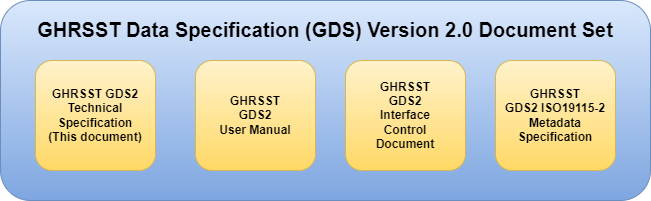
\includegraphics[width=1 \textwidth]{../images/schematicOverview.drawio.png}
%     \caption{Schematic overview of the GHRSST Data Specification Version 2.0 document pack.}
%     \label{fig:schematic_overview}
% \end{figure} % OK: => for the scope of the document
\pagebreak
\section{Overview of GHRSST and the GDS 2.0}
GHRSST [RD-2] is an international consortium representing commercial enterprises, academic
institutions, research organizations, and operational agencies that collaborate to provide accurate,high resolution, and consistently formatted SST observations and analyses from space-based
platforms. This section briefly provides information on the importance of SST, an overview and
history of GHRSST, and context for understanding the GDS 2.0.
\subsection{The Importance of SST}
Sea Surface Temperature at the ocean-atmosphere interface is a fundamental variable for understanding, monitoring and predicting fluxes of heat, momentum and gas at a variety of scales that determine complex interactions between atmosphere and ocean.
The ocean stores heat from the sun and redistributes it from the tropical regions to higher latitudes and to the less dense atmosphere regulating global weather and climate.
Through the hydrological cycle the coupled system controls terrestrial life by redistributing fresh water over the land surface.
From large ocean gyres and atmospheric circulation cells that fuel atmospheric depression systems, storms and hurricanes with their attendant wind waves and storm surges, to local scale phenomena such as the generation of sea breezes and convection clouds, SST at the ocean-atmosphere interface has a significant societal impact.
\par\vspace{0.25cm}
\noindent Accurate knowledge of global SST distribution and temporal variation at finer spatial resolution is needed as a key input to numerical weather prediction (NWP) and numerical ocean prediction (NOP) systems to constrain the modelled upper-ocean circulation and thermal structure at daily, seasonal, decadal and climatic time scales, for the exchange of energy between the ocean and atmosphere in coupled ocean-atmosphere models, and as boundary conditions for ocean forecasting models.
Such models are widely used operationally for various applications including maritime safety, military operations, ecosystem assessments, fisheries support, and tourism.
\par\vspace{0.25cm}
\noindent In addition, well-defined and quantified error estimates of SST are also required for climate time series that can be analysed to reveal the role of the ocean in short and long term climate variability.
A 30 year record of satellite SST observations is available now, that grows on a daily basis.
SST climate data records that are used to provide the GCOS SST Essential Climate Variable (ECV) [RD7], [RD-11], [RD-12] are essential to monitoring and understanding climate variability, climate-ecosystem interactions such as coral reef health and sustainable fisheries management, and critical issues like sea level rise and changing sea ice patterns.
\subsection{GHRSST History}
In 1998, SST data production was considered a mature component of the observing system with demonstrated capability and data products.
However, SST product availability was limited to a few data sets that were large, scientific in format and difficult to exchange in a near real time manner.
Product accuracy was considered insufficient for the emerging NWP and NOP systems.
Uncertainty estimates for SST products were unavailable with SST products complicating their application by the NWP and NOP data assimilation community.
At the same time the number of applications requiring an accurate high resolution SST data stream was growing.
\par\vspace{0.25cm}
Considering these issues, the Global Ocean Data Assimilation Experiment (GODAE) [RD-10] defined the minimum data specification required for use in operational ocean models, stating that SST observations with global coverage, a spatial resolution of 10 km and an accuracy of <0.4 K need to be updated every six hours [RD-10].
\par\vspace{0.25cm}
Despite the network of SST observations from ships and buoys, the only way to achieve these demanding specifications was to make full use of space-based observations.
An integrated and international approach was sought to improve satellite SST measurements, based on four principles:\par\vspace{0.25cm}
\begin{enumerate}
    \item{Respond to user SST requirements through a consensus approach}
    \item{Organize activities according to principles of shared responsibility and subsidiarity, handling matters with the lowest, smallest, or least centralized competent group possible}
    \item{Develop complementarities between independent measurements from earth observation satellites and in situ sensors }
    \item{Maximize synergy benefits of an integrated SST measurement system and end-to-end user service}
\end{enumerate}
\par\vspace{0.25cm}
These foundations enabled the international ocean remote sensing community, marine
meteorologists, Space Agencies, and ocean modellers to combine their energies to meet the GODAE
requirements by establishing the GODAE High Resolution Sea Surface Temperature Pilot Project
(GHRSST-PP). GHRSST-PP established four main tasks relevant to the development of the SST
observing system:
\par\vspace{0.25cm}
\begin{enumerate}
    \item{Improve SST data assembly/delivery}
    \item{Test available SST data sources }
    \item{Perform inter-comparison of SST products }
    \item{Develop applications and data assimilation of SST to demonstrate the benefit of the improved observing system}
\end{enumerate}
\par\vspace{0.25cm}
GHRSST-PP successfully demonstrated that the requirements of GODAE could be met when significant amounts of GHRSST-PP data became available in 2006, and was instrumental in defining the shape and form of the modern-era SST measurement system and user service over the last 10 years [RD-2].
\par\vspace{0.25cm}
At the end of the GODAE period in 2009, the GHRSST-PP evolved into the Group for High Resolution SST (GHRSST). GHRSST built on the successes of the pilot project phase and continued a series of international workshops that were held during 2000-2009. These workshops established a set of user requirements for all GHRSST activities in five areas:
\par\vspace{0.25cm}
\begin{enumerate}
    \item{Scientific development and applications,}
    \item{Operational agency requirements,}
    \item{SST product specifications,}
    \item{Programmatic organization of an international SST service,}
    \item{Developing scientific techniques to improve products and exploit the observing system.}
\end{enumerate}
\par\vspace{0.25cm}
These requirements were critical to establishing the GHRSST framework and work plan, and formed an essential part of the GHRSST evolution. By establishing and documenting clear requirements in a consultative manner at the start of the project and through all stages of its development, GHRSST was able to develop confidently and purposefully to address the needs of the international SST user community
\par\vspace{0.5cm}
\subsection{GHRSST Organization}
Over the last decade, GHRSST established and now continues to provide an internationally distributed suite of user focused services in a sustained Regional/Global Task Sharing (R/GTS) framework [RD-2] that addresses international organizational challenges and recognizes the implementing institutional capacities, capabilities, and funding prospects. Long term stewardship, user support and help services, and standards-based data management and interoperability have been developed and are operated within the R/GTS on a daily basis.
\par\vspace{0.25cm}
GHRSST data flow from numerous Regional Data Assembly Centre\'s (RDACs) to a Global Data Assembly Centre (GDAC) in near real time. Thirty days after observation, the data are transferred to a Long Term Stewardship and Reanalysis Facility (LTSRF). At present, RDACs from across Europe, Japan, Australia, and the United States contribute GHRSST data to the GDAC, operated by the NASA Jet Propulsion Laboratory, which in turn provides the data to the LTSRF operated by the NOAA National Oceanographic Data Center. The GHRSST R/GTS is shown schematically below in \ref{fig:r/gts}.
\begin{figure}[h]
    \centering
    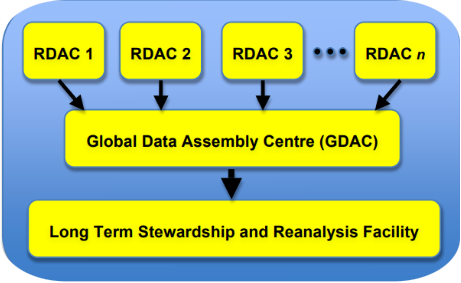
\includegraphics[width=0.75\textwidth]{../images/schematicTaskSharing.drawio.png}
    \caption{Schematic of the GHRSST Regional/Global Task Sharing (R/GTS) framework.}
    \label{fig:r/gts}
\end{figure}
\par\vspace{0.25cm}
Since large-scale GHRSST data production and dissemination commenced in 2006, the GHRSST GDAC and LTSRF have combined to provide over 50,000 users more than 100 terabytes of GHRSST data. Over 28 terabytes of data are in NODC\'s LTSRF holdings with another approximately 10 Terabyte added each year. The detailed interactions of the R/GTS components are described in the GHRSST Interface Control Document [AD-1].
Each component of the R/GTS is independently managed and operated by different institutions and agencies. The R/GTS itself is coordinated by the international GHRSST Science Team, which receives guidance and advice from the GHRSST Advisory Council. A GHRSST Project Office coordinates the overall framework. A full discussion of GHRSST over the last 10 years is reported in [RD-2] and [RD-3].
\subsection{Overview of the GDS 2.0}
The GHRSST R/GTS was made possible through the establishment of a rigorous GHRSST Technical Data Specification (GDS), which instructed international satellite data providers on how to process satellite data streams, defined the format and content of the data and metadata, and documented the basic approaches to providing uncertainty estimates and auxiliary data sets. The GHRSST-PP established the first GDS (v1.6) [RD-1], which formed the basis of all GHRSST data production from 2005 through 2011. In 2010 the Version 2 of the GDS described in this document will go into operations following a phased implementation schedule.
\par\vspace{0.25cm}
All GHRSST products entering the R/GTS must strictly follow the common GDS when generating L2P, L3, L4, and GMPE data. As a result, users with common tools to read data from one RDAC can securely use data from any of the others as well as the GDAC and LTSRF without a need to re-code. Table 6-1 provides a summary of GDS 2.0 data products and their basic characteristics.
\par\vspace{0.25cm}
The remainder of this document provides the detailed specifications for GHRSST L2P, L3, L4, and GMPE products, their file naming convention, metadata requirements, and all necessary tables, conventions, and best practices for creating and using GHRSST data.
\newp % OK: => provides overview on the ECCO product
\pagebreak
\section{ECCO Data Filenames and Supporting Conventions}


ECCO Version 4 Release 4 (V4r4) follows a structured filename convention to organize its extensive datasets. The filenames encode essential information about the dataset's content, grid type, temporal resolution, and version. Below is an overview of the naming convention.

\subsection{General filename Structure}
\par \vspace{0.25cm}

\par For ECCO dataset product files:

\par \vspace{0.5cm}
\begin{center}
\small{\textbf{\fontfamily{lmtt}\selectfont{[ShortName]\_[TemporalResolution]\_[Indicative Time]\_ECCO\_[Version]\_[GridType].<File Type>}}}
\end{center}
\par \vspace{0.5cm}
\par For ECCO data geometry and grid files:

\par \vspace{0.5cm}
\begin{center}
    \small{\textbf{\fontfamily{lmtt}\selectfont{[ShortName]\_ECCO\_[Version]\_[GridType].<File Type>}}}
\end{center}
% \texttt
\par \vspace{0.25cm}

\begin{center}
\begin{tabular}{m{0.18\textwidth} m{0.75\textwidth}}
    \multicolumn{1}{c}{\textbf{Keypoins}} & \multicolumn{1}{c}{\textbf{Description}} \\ \hline
    ShortName: & Describes the dataset variable (e.g., SSH for sea surface height, TEMP\_SALINITY for temperature and salinity). \\ \hline 
    TemporalResolution: & Indicates the time averaging or snapshot type (e.g., DAILY, MONTHLY, SNAP). \\ \hline
    GridType : & Specifies the grid used (e.g., \textbf{native\_llc90} for the native ECCO grid or \textbf{laton\_0p50deg} for interpolated 0.5 \textdegree lat-lon grid). It can also be a specific information such as \textbf{1D} to indication the one-dimentional dataset files over the full period of ECCO data availability.\\ \hline
    Version: &  Identifies the ECCO release version (e.g., V4r4). \\ \hline
    Indicative Time: & Encodes the time period covered by the file (e.g., monthly files use YYYY-MM, daily files use YYYY-MM-DD) \\ \hline
    File Type & netCDF or Zarr data format. \\ \hline
\end{tabular}
\end{center}

\par \vspace{0.25cm}
\subsection{Examples}
\par Daily atmosphere surface temperature, humidity, winds, and pressure on the lat-lon-cap 90 (llc90)
native model grid (first) and on the interpolated regular 0.5-degree lat-lon grid (second) from ECCO V4r4 on 2017-12-29.
\begin{itemize}
    \item ATM\_SURFACE\_TEMP\_HUM\_WIND\_PRES\_day\_mean\_2017-12-29\_ECCO\_V4r4\_native\_llc0090.nc
    \item ATM\_SURFACE\_TEMP\_HUM\_WIND\_PRES\_day\_mean\_2017-12-29\_ECCO\_V4r4\_latlon\_0p50deg.nc
\end{itemize}

\par Dynamic sea surface height interpolated on the latlon regular 0.5-degree model grid from ECCO V4r4 on 2017-12-29.

\begin{itemize}
    \item SEA\_SURFACE\_HEIGHT\_day\_mean\_2017-12-29\_ECCO\_V4r4\_native\_llc0090.nc
\end{itemize}

\par One-dimentional field of global mean atmospheric surface pressure over the ocean and sea-ice fromthe ECCO V4r4.
\begin{itemize}
    \item GLOBAL\_MEAN\_ATM\_SURFACE\_PRES\_snap\_ECCO\_V4r4\_1D.nc
\end{itemize}

\par Geometric parameters for the regular 0.5-degree lat-lon grid from ECCO V4r4.
\begin{itemize}
    \item GRID\_GEOMETRY\_ECCO\_V4r4\_latlon\_0p50deg.nc
\end{itemize}

%%% Arret ici !!!!!! Modify!!!

% \subsection{1 Overview of Filename Convention and Example Filenames}
% The filenaming convention for the GDS 2.0 is shown below. 
% \par \vspace{0.25in}

% \small{\texttt{<Dataset name>_<>_<Indicative Time>-<RDAC>-<Processing Level>\_GHRSST-<SST Type>-
% <Product String>-<Additional Segregator>-v<GDS Version>-fv<File Version>.<File Type>}}
% \par \vspace{0.25in}

% The variable components within braces (“< >”) are summarized in Table 7-1 below and detailed in the
% \textbf{should not} be used in any GHRSST code or the <Additional Segregator> element. Example
% filenames are given later in this section. While no strict limit to filename length is mandated, RDACs
% are encouraged to keep the length to less than 240 characters to increase readability and usability.

% %Table 7-1. GDS 2.0 Filenaming convention components
% \begin{longtable}{|p{0.2\textwidth}|p{0.3\textwidth}|p{0.5\textwidth}|}
% \caption{GDS 2.0 Filenaming convention components}
% \label{tab:filenaming conventions}
% \\ \hline
% \rowcolor{lightgray}
% \textbf{Name} & \textbf{Definition} & \textbf{Description} \\ \hline 
% \endfirsthead
% <Indicative Date> & YYYYMMDD & The identifying date for this data set. See Section 7.2. \\ \hline
% <Indicative Time> & HHMMSS & The identifying time for this data set. The time used is dependent on the <Processing Level> of
% the data set: L2P: start time of granule 
% \begin{itemize}
%  \item{L3U: start time of granule}
%  \item{L3C and L3S: centre time of the collation window}
%  \item{L4 and GMPE: nominal time of analysis}
% \end{itemize}
% All times should be given in UTC. See Section 7.3. \\ \hline
% <RDAC> & The RDAC where the file was created & The Regional Data Assembly Centre (RDAC)code, listed in Section 7.4. \\ \hline
% <Processing Level> & The data processing level code (L2P, L3U, L3C, L3S, or L4) & 
% The data processing level code, defined in Section 7.5. \\ \hline
% <SST Type> & The type of SST data included in the file. & 
% Conforms to the GHRSST definitions for SST, defined in Section 7.6 \\ \hline

% <Product String> &
% A character string identifying the
% SST product set. The string is
% used uniquely within an RDAC
% but may be shared across
% RDACs. & 
% The unique “name” within an RDAC of the
% product line. See Section 7.7 for the product
% string lists, one each for L2P, L3, L4, and GMPE
% products. See Section 7.7. \\ \hline

% <Additional Segregator> &
% Optional text to distinguish
% between files with the same
% <Product String>. Dashes are
% not allowed within this element. &
% This text is used since the other filename
% components are sometimes insufficient to
% uniquely identify a file. For example, in L2P or
% L3U (un-collated) products this is often the
% original file name or processing algorithm. Note,
% underscores should be used, not dashes. For L4
% files, this element should begin with the
% appropriate regional code as defined in Section 7.8. This component is optional but must be used
% in those cases were non-unique filenames would otherwise result. \\ \hline

% <GDS Version> & nn.n & Version number of the GDS used to process the file. For example, GDS 2.0 = “02.0”. \\ \hline
% <File Version> & xx.x & Version number for the file, for example, “01.0”. \\ \hline

% <File Type> & netCDF data file suffix (nc) or ISO metadata file suffix (xml) & 
% Indicates this is a netCDF file containing data or its corresponding ISO-19115 metadata record in XML.\\ \hline

% \end{longtable}

% \subsubsection{L2\_GHRSST Filename Example}
% 20070503132300-NAVO-L2P\_GHRSST-SSTblend-AVHRR17\_L-SST\_s0123\_e0135-v02.0-fv01.0.nc \par
% The above file contains GHRSST L2P blended SST data for 03 May 2007, from AVHRR LAC data
% collected from the NOAA-17 platform. The granule begins at 13:23:00 hours. It is version 1.0 of the
% file and was produced by the NAVO RDAC in accordance with the GDS 2.0. The <Additional
% Segregator> text is “SST\_s0123\_e0135”. \par

% \subsubsection{L3\_GHRSST Filename Example}
% 20070503110153-REMSS-L3C\_GHRSST-SSTsubskin-TMI-tmi\_20070503rt-v02.0-fv01.0.nc \par
% The above file was produced by the REMSS RDAC and contains collated L3 sub-skin SST data from
% the TMI instrument for 03 May 2007. The collated file has a centre time of at 11:01:53 hours. It is
% version 1.0 of the file and was produced according to GDS 2.0 specifications. Its <Additional
% Segregator> text is “tmi\_20070503rt”. \par

% \subsubsection{L4\_GHRSST Filename Example}
% 20070503120000-UKMO-L4\_GHRSST-SSTfnd-OSTIA-GLOB-v02.0-fv01.0.nc \par
% The above file contains L4 foundation SST data produced at the UKMO RDAC using the OSTIA
% system. It is global coverage, contains data for 03 May 2007, was produced to GDS 2.0 specifications
% and is version 1.0 of the file. The nominal time of the OSTIA analysis is 12:00:00 hours. \par


% \subsection{<Indicative Date>}
% The identifying date for this data set, using the format YYYYMMDD, where YYYY is the four-digit year,
% MM is the two-digit month from 01 to 12, and DD is the two-digit day of month from 01 to 31. The date
% used should best represent the observation date for the dataset. \par

% \subsection{<Indicative Time>}
% The identifying time for this data set in UTC, using the format HHMMSS, where HH is the two-digit
% hour from 00 to 23, MM is the two-digit minute from 00 to 59, and SS is the two-digit second from 00 to
% 59. The time used is dependent on the <Processing Level> of the data set: \par \vspace{0.5in}

% L2P: start time of granule \\
% L3U: start time of granule \\ 
% L3C and L3S: centre time of the collation window \\ 
% L4 and GMPE: nominal time of analysis \par \vspace{0.1in}
% All times should be given in UTC and should be chosen to best represent the observation time for this
% dataset. Note: RDACs should ensure the applications they use to determine UTC proprerly account
% for leap seconds.

% \subsection{<RDAC>}
% Codes used for GHRSST Regional Data Assembly Centres (RDACs) are provided in the table below.
% New codes are assigned by the GHRSST Data And Systems Technical Advisory Group (DAS-TAG)
% and entered into the table upon agreement by the GDAC, LTSRF, and relevant RDACs. \par


% % Table 7-2: Regional Data Assembly Centre (RDAC) code table.
% \begin{table}[h]
% \centering
% \caption{Regional Data Assembly Centre (RDAC) code table}
% \label{tab:RDAC code table}
% \begin{tabular}{|p{0.2\textwidth}|p{0.8\textwidth}|}
% \hline
% \rowcolor{lightgray}
% RDAC Code & GHRSST RDAC Name \\ \hline
% ABOM & Australian Bureau of Meteorology \\ \hline
% CMC & Canadian Meteorological Centre \\ \hline
% DMI & Danish Meteorological Institute \\ \hline
% EUR & European RDAC \\ \hline
% GOS & Gruppo di Oceanografia da Satellite \\ \hline
% JPL & JPL Physical Oceanography Distributed Active Archive Center \\ \hline
% JPL\_OUROCEAN & JPL OurOcean Project \\ \hline
% METNO & Norwegian Meteorological Institute \\ \hline
% MYO & MyOcean \\ \hline
% NAVO & Naval Oceanographic Office \\ \hline
% NCDC & NOAA National Climatic Data Center \\ \hline
% NEODAAS & NERC Observation Data Acquisition and Analysis Service \\ \hline
% NOC & National Oceanography Centre, Southampton \\ \hline
% NODC & NOAA National Oceanographic Data Center \\ \hline
% OSDPD & NOAA Office of Satellite Data Processing and Distribution \\ \hline
% OSISAF & EUMETSAT Ocean and Sea Ice Satellite Applications Facility \\ \hline
% REMSS & Remote Sensing Systems, CA, USA \\ \hline
% RSMAS & University of Miami, RSMAS \\ \hline
% UKMO & UK Meteorological Office \\ \hline
% UPA & United Kingdom Multi-Mission Processing and Archiving Facility \\ \hline
% ESACCI & ESA SST Climate Change Initiative \\ \hline
% JAXA & Japan Aerospace Exploration Agency \\ \hline
% New codes & Please contact the GHRSST international Project Office if you require new
% codes to be included in future revisions of the GDS. \\ \hline

% \end{tabular}
% \end{table}


% \subsection{<Processing Level>}
% Satellite data processing level definitions can lead to ambiguous situations, especially regarding the
% distinction between L3 and L4 products. GHRSST identified the use of analysis procedures to fill gaps
% where no observations exist to resolve this ambiguity. Within GHRSST filenames, the <Processing
% Level> codes are shown below in Table 7-3. GHRSST currently establishes standards for L2P, L3U,
% L3C, L3S, and L4 (GHRSST Multi-Product Ensembles known as GMPE are a special kind of L4
% product for which GHRSST also provides standards). \par

% % Table 7-3:  GHRSST Processing Level Conventions and Codes
% \begin{table}[h]
% %\centering
% \caption{GHRSST Processing Level Conventions and Codes}
% \label{tab:GHRSST Processing Level Conventions and Codes}
% \begin{tabular}{|p{0.1\textwidth}|p{0.15\textwidth}|p{0.75\textwidth}|}
% \hline
% \rowcolor{lightgray}
% \textbf{Level} & \textbf{<Processing Level> Code} & \textbf{Description} \\ \hline

% Level 0 & L0 &
% Unprocessed instrument and payload data at full resolution. GHRSST
% does not make recommendations regarding formats or content for data
% at this processing level. \\ \hline

% Level 1A & L1A & 
% Reconstructed unprocessed instrument data at full resolution, time
% referenced, and annotated with ancillary information, including
% radiometric and geometric calibration coefficients and geo-referencing
% parameters, computed and appended, but not applied, to L0 data.
% GHRSST does not make recommendations regarding formats or
% content for data at this processing level. \\ \hline

% Level 1B & L1B & 
% Level 1A data that have been processed to sensor units. GHRSST
% does not currently make recommendations regarding formats or content
% for L1B data. \\ \hline

% Level 2 & Preprocessed L2P &
% Geophysical variables derived from Level 1 source data at the same
% resolution and location as the Level 1 data, typically in a satellite
% projection with geographic information. These data form the
% fundamental basis for higher-level GHRSST products and require
% ancillary data and uncertainty estimates. \\ \hline

% Level 3 & L3U L3C L3S & Level 2 variables mapped on a defined grid with reduced requirements for ancillary data. 
% Uncertainty estimates are still mandatory. Three
% types of L3 products are defined:
% \begin{itemize}
% \item{Un-collated (L3U): L2 data granules remapped to a space grid without combining any observations from overlapping orbits}
% \item {Collated (L3C): observations combined from a single instrument into a space-time grid}
% \item {Super-collated (L3S): observations combined from multiple instruments into a space-time grid.}
% \end{itemize}
% Note that L3 GHRSST products do not use analysis or interpolation
% procedures to fill gaps where no observations are available. \\ \hline

% Level 4 & L4 &
% Data sets created from the analysis of lower level data that result in
% gridded, gap-free products. SST data generated from multiple sources
% of satellite data using optimal interpolation are an example of L4
% GHRSST products. GMPE products are a type of L4 dataset. \\  \hline

% Note that within GHRSST, all L2P files require a full set of extensive ancillary data such as wind
% speeds and times of observation that are provided as \'dynamic flags\' that users can manipulate to
% filter data according to their own quality criteria. L2P files form the basis of higher-level products and
% are often the best level products for data assimilation. The requirement for dynamic flags is particularly
% important in this context. Higher-level L3 products are often intended for general use or created for
% input to Level 4 analysis systems so the requirement for extensive ancillary data is reduced. Since
% some GHRSST RDACs only process data natively on grids (especially in the case of geostationary
% platform observations), the GDS 2.0 L3 specification is flexible enough to allow for the creation of L3
% files which meet all the content requirements of a L2P file. In all L2P and L3 cases, bias and standard
% deviation uncertainty estimates are mandatory. \par

% The distinction between L3 GHRSST and L4 GHRSST data is made primarily on whether or not any
% gap-filling techniques are employed, not on whether data from multiple instruments is used in the L3
% product. If no gap filling procedure (such as optimal interpolation) is used, then the product remains a
% L3 GHRSST product. GHRSST defines three kinds of L3 files: un-collated (L3U), collated (L3C), and
% super-collated (L3S). If gap filling is used to fill all observations gaps, then the resulting gap-free data
% are considered L4 GHRSST data products. \par
% \end{tabular}
% \end{table}

%%% Arret ici !!!!!!

% \subsection{<SST Type>}
% In conjunction with the NetCDF Climate and Forecast (CF) community [AD-9] the GHRSST Science
% Team agreed on the CF standard names for “SST” shown in the following figure and described in
% more detail below. The names were first included in CF-1.3, and the current version (CF-1.4) of the
% standard name table that can be found in [AD-8]. In addition, the GHRSST Science Team agreed to
% use the CF Naming Convention [AD-3] for variable names that do not already exist as part of the CF
% Convention. CF definitions are used in the GDS and across GHRSST and are shown schematically in
% Figure 7-1. The different kinds of SST are detailed later in this section and the relevant <SST Type>
% codes to be used in the filenames are provided. \par \vspace{1in}

% % Figure 7-1. Overview of SST measurement types used within GHRSST
% \begin{figure}[h]
%     \caption{Overview of SST measurment types used within GHRSST}
%     \label{fig:Overview of SST measurment types used within GHRSST}
% \end{figure}
% \textbf{Figure 7-1. Overview of SST measurement types used within GHRSST.} \par
% CF Definition: \emph{sea\_surface\_temperature is usually abbreviated as "SST". It is the temperature of sea
% water near the surface (including the part under sea-ice, if any), and not the interface temperature,
% whose standard name is surface\_temperature. For the temperature of sea water at a particular depth
% or layer, a data variable of sea\_water\_temperature with a vertical coordinate axis should be used.} \par
% Additional Details: The sea surface skin temperature (SSTskin) as defined above represents the
% actual temperature of the water across a very small depth of approximately 20 micrometers. This
% definition is chosen for consistency with the majority of infrared satellite and ship mounted radiometer
% measurements. \par

% \textbf{Sea\_surface\_subskin\_temperature (GHRSST <SST Type>: SSTsubskin):}\par
% CF Definition: \emph{The surface called "surface" means the lower boundary of the atmosphere. The sea
% surface subskin temperature is the temperature at the base of the conductive laminar sub-layer of the
% ocean surface, that is, at a depth of approximately 1 - 1.5 millimetres below the air-sea interface. For
% practical purposes, this quantity can be well approximated to the measurement of surface temperature
% by a microwave radiometer operating in the 6 - 11 gigahertz frequency range, but the relationship is
% neither direct nor invariant to changing physical conditions or to the specific geometry of the
% microwave measurements. Measurements of this quantity are subject to a large potential diurnal cycle
% due to thermal stratification of the upper ocean layer in low wind speed high solar irradiance
% conditions.}\par
% Additional Details: The sea surface subskin temperature (SSTsubskin) represents the temperature at
% the base of the thermal skin layer. The difference between SSTint and SSTsubskin is related to the
% net flux of heat through the thermal skin layer. SSTsubskin is the temperature of a layer approximately
% 1 mm thick at the ocean surface.\par

% \textbf{Sea\_water\_temperature (GHRSST <SST Type>: SSTdepth or SSTz):}\par
% CF Definition: \emph{The general term, "bulk" sea surface temperature, has the standard name
% sea\_surface\_temperature with no associated vertical coordinate axis. The temperature of sea water at
% a particular depth (other than the foundation level) should be reported using the standard name
% sea\_water\_temperature and, wherever possible, supplying a vertical coordinate axis or scalar
% coordinate variable.}\par
% Additional Details: Sea water temperature (SSTdepth or SSTz, for example SST1.5m) is the terminology
% adopted by GHRSST to represent in situ measurements near the surface of the ocean that have
% traditionally been reported simply as SST or "bulk" SST. For example SST6m would refer to an SST
% measurement made at a depth of 6 m. Without a clear statement of the precise depth at which the
% SST measurement was made, and the circumstances surrounding the measurement, such a sample
% lacks the information needed for comparison with, or validation of satellite-derived estimates of SST
% using other data sources. The terminology has been introduced to encourage the reporting of depth
% (z) along with the temperature.\par
% All measurements of water temperature beneath the SSTsubskin are obtained from a wide variety of
% sensors such as drifting buoys having single temperature sensors attached to their hull, moored buoys
% that sometimes include deep thermistor chains at depths ranging from a few meters to a few thousand
% meters, thermosalinograph (TSG) systems aboard ships recording at a fixed depth while the vessel is 
% underway, Conductivity Temperature and Depth (CTD) systems providing detailed vertical profiles of
% the thermohaline structure used during hydrographic surveys and to considerable depths of several
% thousand meters, and various expendable bathythermograph systems (XBT). In all cases, these
% temperature observations are distinct from those obtained using remote sensing techniques and
% measurements at a given depth should be referred to as sea\_water\_temperature qualified by a depth
% in meters rather than sea surface temperatures. The situation is complicated further when one
% considers ocean model outputs for which the SST may be the mean SST over a layer of the ocean
% several tens of meters thick.\par

% \textbf{Sea\_surface\_foundation\_temperature (GHRSST <SST Type>: SSTfnd):}\par
% CF Definition: \emph{The surface called "surface" means the lower boundary of the atmosphere. The sea
% surface foundation temperature is the water temperature that is not influenced by a thermally stratified
% layer of diurnal temperature variability (either by daytime warming or nocturnal cooling). The
% foundation temperature is named to indicate that it is the temperature from which the growth of the
% diurnal thermocline develops each day, noting that on some occasions with a deep mixed layer there
% is no clear foundation temperature in the surface layer. In general, sea surface foundation temperature
% will be similar to a night-time minimum or pre-dawn value at depths of between approximately 1 and 5
% meters. In the absence of any diurnal signal, the foundation temperature is considered equivalent to
% the quantity with standard name sea\_surface\_subskin\_temperature. The sea surface foundation
% temperature defines a level in the upper water column that varies in depth, space, and time depending
% on the local balance between thermal stratification and turbulent energy and is expected to change
% slowly over the course of a day. If possible, a data variable with the standard name
% sea\_surface\_foundation\_temperature should be used with a scalar vertical coordinate variable to
% specify the depth of the foundation level. Sea surface foundation temperature is measured at the base
% of the diurnal thermocline or as close to the water surface as possible in the absence of thermal
% stratification. Only in situ contact thermometry is able to measure the sea surface foundation
% temperature. Analysis procedures must be used to estimate sea surface foundation temperature value
% from radiometric satellite measurements of the quantities with standard names
% sea\_surface\_skin\_temperature and sea\_surface\_subskin\_temperature. Sea surface foundation
% temperature provides a connection with the historical concept of a "bulk" sea surface temperature
% considered representative of the oceanic mixed layer temperature that is typically represented by any
% sea temperature measurement within the upper ocean over a depth range of 1 to approximately 20
% meters. The general term, "bulk" sea surface temperature, has the standard name
% sea\_surface\_temperature with no associated vertical coordinate axis. Sea surface foundation
% temperature provides a more precise, well-defined quantity than "bulk" sea surface temperature and,
% consequently, is more representative of the mixed layer temperature. The temperature of sea water at
% a particular depth (other than the foundation level) should be reported using the standard name
% sea\_water\_temperature and, wherever possible, supplying a vertical coordinate axis or scalar
% coordinate variable.}\par
% Additional Details: Through the definition of the CF standard names, GHRSST is attempting to
% discourage the use of the term “bulk SST”, replacing it instead with sea\_water\_temperature
% (SSTdepth) and a depth coordinate, or sea\_surface\_foundation\_temperature (SSTfnd) and a depth
% coordinate if possible, if the observation comes from the base of the diurnal thermocline.\par

% \textbf{Blended SST (GHRSST <SST Type>: SSTblend):}\par
% In addition to the CF standard names defined above, GHRSST also uses the term “Blended SST” for
% ambiguous cases when the depth or type of SST is not well known. This ambiguity in depth may arise
% in some L4 analysis products that merge multiple types of SST from satellite and in situ observations.
% Note, however, that many L4 analysis systems do attempt to specifically create a sea surface
% foundation temperature, SSTfnd.\par
% The SST codes and CF standard names defined above and used within GHRSST are summarized
% along with their key characteristics in Table 7-4.\par

% %Table 7-4. GHRSST <SST Type> code and summary table
% \begin{table}[h]
%     \caption{ECCO <SST Type> code and summary table}
%     \label{tab:ECCO <SST Type> code and summary table}
%     \begin{tabular}{|p{0.1\textwidth}|p{0.65\textwidth}|p{0.1\textwidth}|p{0.15\textwidth}|}
%     \rowcolor{lightgray}
%     \textbf{ECCO <SST Type>} & \textbf{CF Standard Name} & \textbf{Approximate Depth} & \textbf{Typically Observed
%     by...} \\ \hline
%     SSTint & \texttt{sea\_surface\_temperature} &  0 meters & Not presently measureable \\ \hline
%     SSTskin & \texttt{sea\_surface\_skin\_temperature} & 10 - 20 micrometers & Infrared radiometers
%     operating in a range
%     of wavelengths form
%     3.7 to 12
%     micrometers \\ \hline

%     SSTsubskin & \texttt{sea\_surface\_subskin\_temperature} & 1 - 1.5 millimeters & Microwave radiometers operating in a range
%     of frequencies from
%     6-11 gigahertz \\ \hline

%     SSTdepth & \texttt{sea\_water\_temperature} & Specified by
%     vertical
%     coordinate
%     (e.g., SST\_{5m}) & In situ observing systems \\ \hline

%     SSTfnd & \texttt{sea\_surface\_foundation\_temperature} & 1-5 meters pre-dawn & 
%     In situ observing systems \\ \hline

%     SSTblend & None &  Unknown & Blend of satellite and in situ observations \\ \hline
    
%     \end{tabular}
% \end{table}


% \subsection{<Product String>}
% The current set of GHRSST product strings is listed in tables below, in one table each for L2P (Table
% 7-5), L3 (Table 7-6), L4 (Table 7-7) and GMPE (Table 7-8) products. Included in the L2P table are
% also codes for satellite platforms and sensors. New strings are entered into the tables upon
% registration by the DAS-TAG and agreement by the GDAC, LTSRF, and relevant RDACs. These
% product strings are used within the GHRSST filename convention and within the GHRSST unique data
% set codes described in Section 7.9. The satellite platform and satellite sensor entries are also used in
% the netCDF global attributes, \texttt{platform} and \texttt{sensor}, for all GHRSST product files. See Section 8.2
% for more information on the required \texttt{global attributes}. \par

 % OK: => Provides info on ECCO data files nomenclature and variable conventions.
\pagebreak
\section{ECCO Data Product File Structure}
\subsection{Overview of the ECCO Data netCDF File Format}

ECCO data files preferentially use the \textbf{netCDF-4} format. These ECCO formatted data comply with the Climate and Forecast (CF) Conventions, because these conventions provide a practical standard for storing oceanographic data in a robust, easily-preserved for the long-term, and interoperable manner. The CF-compliant netCDF data format is flexible, self-describing, and has been adopted as a de facto standard for many operational and scientific oceanography systems. Both netCDF and CF are actively maintained
including significant discussions and inputs from the oceanographic community (see \url{http://cfpcmdi.llnl.gov/discussion/index_html}). 
The CF convention generalizes and extends the Cooperative Ocean/Atmosphere Research Data Service (COARDS, [AD-4]) Convention but relaxes the COARDS constraints on dimension order and specifies methods for reducing the size of datasets. The purpose
of the CF Conventions is to require conforming datasets to contain sufficient metadata so that they are
self-describing, in the sense that each variable in the file has an associated description of what it
represents, physical units if appropriate, and that each value can be located in space (relative to earthbased coordinates) and time. In addition to the CF Conventions, ECCO formatted files follow some of the recommendations of the Unidata Attribute Convention for Dataset Discovery. \par \vspace{0.1in}

In the context of netCDF, a variable refers to data stored in the file as a vector or as a
multidimensional array. Within the netCDF file, global attributes are used to hold information that applies to the whole file, such
as the data set title. Each individual variable has its own attributes, referred to as variable attributes. These variable attributes define, for example, an axis, long$\_$name, standard$\_$name, units, a descriptive version of the variable name, and a fill value (if apply), which is used to indicate array elements that do not
contain valid data.

\par \vspace{0.1in} Overall, the ECCO netCDF  files are structured in five (5) blocks: 
\begin{itemize}
    \item Dimensions
    \item Coordinates
    \item Data variables
    \item Indexes
    \item Attributes
\end{itemize}

\subsection{ECCO netCFD Global Attributes}

\subsection{ECCO netCFD Coordinates, Dimensions and Variabiles Attributes}
\par Provide dimension across all datasets

\begin{longtable}{|m{0.15\textwidth}|m{0.15\textwidth}|m{0.7\textwidth}|}
    \hline \endhead \hline \endfoot'
    Dimensions & Length & Description \\ \hline
    i & "to be filled" & "to be filled" \\ \hline
    i\_g & "to be filled" & "to be filled" \\ \hline
    j & "to be filled" & "to be filled" \\ \hline
    j\_g & "to be filled" & "to be filled" \\ \hline
    k & "to be filled" & "to be filled" \\ \hline
    k\_u & "to be filled" & "to be filled" \\ \hline
    k\_l & "to be filled" & "to be filled" \\ \hline
    k\_p1 & "to be filled" & "to be filled" \\ \hline
    tile & "to be filled" & "to be filled" \\ \hline
    nb & "to be filled" & "to be filled" \\ \hline
    nv & "to be filled" & "to be filled" \\ \hline    
\end{longtable}
\subsection{ECCO Data netCDF Coordinates and Variabiles Attributes}
\par Provide Coordinates and variabiles attribute across all datasets
    
\subsection{ECCO Data netCDF Indexes}
\par Provide a definition for the meaning of "indexes" for the netCDF files
\subsection{ECCO Data netCDF Globale Attributes}

\par Provide Globale attribute for the netCDF files across all datasets

% \subsection{GDS 2.0 netCDF Global Attributes}
% Table 8-1 below summarizes the global attributes that are mandatory for every GDS 2.0 netCDF data
% file. More details on the CF-mandated attributes (as indicated in the Source column) are available at:
% \url{http://cf-pcmdi.llnl.gov/documents/cf-conventions/1.4/cf-conventions.html#attribute-appendix} and
% information on the ACDD recommendations is available at
% \url{http://www.unidata.ucar.edu/software/netcdf-java/formats/DataDiscoveryAttConvention.html}.
% \par \vspace{0.1in}



% % Table 8-1 Mandatory global attributes for GDS 2.0 netCDF data files
\begin{longtable}{|p{0.276\textwidth}|p{0.092\textwidth}|p{0.46\textwidth}|p{0.092\textwidth}|}
\caption{Mandatory global attributes for GDS 2.0 netCDF data files}
\label{tab:global-attributes} \\ 
\hline \endhead
\hline \endfoot
\rowcolor{lightgray} \textbf{Global Attribute Name} & \textbf{Type} & \textbf{Description} & \textbf{Source} \\ \hline
\rowcolor{LightCyan} acknowledgement & string & A place to acknowledge various types of support for the project that produced this data. & ACDD \\ \hline

\rowcolor{LightCyan} cdm\_data\_type & string & The data type, as derived from Unidata's Common Data Model Scientific Data types and understood by THREDDS. (This is a THREDDS "dataType", and is different from the CF NetCDF attribute 'featureType', which indicates a Discrete Sampling Geometry file in CF.) & ACDD \\ \hline

\rowcolor{LightCyan} comment & string & Miscellaneous information about the data, not captured elsewhere. This attribute is defined in the CF Conventions. & CF, ACDD \\ \hline

\rowcolor{LightCyan} conventions & string & A text string identifying the netCDF conventions followed (e.g., CF-1.4, ACDD 1-3). &  \\ \hline

\rowcolor{LightCyan} creator\_email & string & The email address of the person (or other creator type specified by the creator\_type attribute) principally responsible for creating this data. & ACDD \\ \hline

\rowcolor{LightCyan} creator\_name & string & The name of the person (or other creator type specified by the creator\_type attribute) principally responsible for creating this data. & ACDD \\ \hline

\rowcolor{LightCyan} creator\_url & string & The URL of the of the person (or other creator type specified by the creator\_type attribute) principally responsible for creating this data. & ACDD \\ \hline

\rowcolor{LightCyan} date\_created & string & The date on which this version of the data was created. & ACDD \\ \hline

\rowcolor{LightCyan} easternmost\_longitude & float & Decimal degrees east, range -180 to +180. This is equivalent to ACDD geospatial\_lon\_max. & podaac \\ \hline

\rowcolor{LightCyan} geospatial\_lat\_resolution & float & Latitude Resolution in units matching geospatial\_lat\_units. & ACDD \\ \hline

\rowcolor{LightCyan} geospatial\_lat\_units & string & Units of the latitudinal resolution. Typically "degrees\_north" & ACDD \\ \hline

\rowcolor{LightCyan} geospatial\_lon\_resolution & float & Longitude Resolution in units matching geospatial\_lon\_resolution & ACDD \\ \hline

\rowcolor{LightCyan} geospatial\_lon\_units & string & Units of the longitudinal resolution. Typically "degrees\_east" & ACDD \\ \hline

\rowcolor{LightCyan} history & string & The name of the institution principally responsible for originating this data. This attribute is recommended by the CF convention. & CF, ACDD \\ \hline

\rowcolor{LightCyan} id & string & An identifier for the data set, provided by and unique within its naming authority. The combination of the "naming authority" and the "id" should be globally unique, but the id can be globally unique by itself also. IDs can be URLs, URNs, DOIs, meaningful text strings, a local key, or any other unique string of characters. The id should not include white space characters. & ACDD \\ \hline

\rowcolor{LightCyan} institutions & string & The name of the institution principally responsible for originating this data. This attribute is recommended by the CF convention. & CF, ACDD \\ \hline

\rowcolor{LightCyan} keywords & string & GCMD Science Keyword(s) & ACDD \\ \hline

\rowcolor{LightCyan} keywords\_vocabulary & string & The unique name or identifier of the vocabulary from which keywords are taken. e.g., the NASA Global Change Master Directory (GCMD) Science Keywords. & ACDD \\ \hline

\rowcolor{LightCyan} license & string & Provide the URL to a standard or specific license, enter "Freely Distributed" or "None", or describe any restrictions to data access and distribution in free text. & ACDD \\ \hline

\rowcolor{LightCyan} Metadata\_Conventions & string & A comma-separated list of the conventions that are followed by the dataset.  & ACDD \\ \hline

\rowcolor{LightCyan} metadata\_link & string & Link to collection metadata record at archive & ACDD \\ \hline

\rowcolor{LightCyan} naming\_authority & string & The organization that provides the initial id (see above) for the dataset. The naming authority should be uniquely specified by this attribute via reverse-DNS naming convention. & ACDD \\ \hline

\rowcolor{LightCyan} netcdf\_version\_id  & string & Version of netCDF libraries used to create this file. For example, "4.1.1" & GDS \\ \hline

\rowcolor{LightCyan} northernmost\_latitude & float & Decimal degrees north, range -90 to +90. This is equivalent to ACDD geospatial\_lat\_max. & GDS \\ \hline

\rowcolor{LightCyan} processing\_level & string & A textual description of the processing (or quality control) level of the data. & ACDD \& GDS \\ \hline

\rowcolor{LightCyan} product\_version & string & The product version of this data file & GDS \\ \hline

\rowcolor{LightCyan} project & string & The name of the project(s) principally responsible for originating this data. & ACDD \\ \hline

\rowcolor{LightCyan} publisher\_email & string & The email address of the person (or other entity specified by the publisher\_type attribute) responsible for publishing the data file or product to users, with its current metadata and format. & ACDD \\ \hline

\rowcolor{LightCyan} publisher\_name & string & The name of the person (or other entity specified by the publisher\_type attribute) responsible for publishing the data file or product to users, with its current metadata and format. & ACDD \\ \hline

\rowcolor{LightCyan} publisher\_url & string & The URL of the person (or other entity specified by the publisher\_type attribute) responsible for publishing the data file or product to users, with its current metadata and format. & ACDD \\ \hline

\rowcolor{LightCyan} references & string & Published or web-based references that describe the data or methods used to produce it. Recommend URIs (such as a URL or DOI) for papers or other references. This attribute is defined in the CF conventions. & ACDD \\ \hline

\rowcolor{LightCyan} source & string & Method of production of the original data. & CF \\ \hline

\rowcolor{LightCyan} sourthernmost\_latitude & float & Decimal degrees north, range -90 to +90. This is equivalent to ACDD geospatial\_lat\_min. & GDS \\ \hline

\rowcolor{LightCyan} spatial\_resolution & string & A string describing the approximate resolution of the product. & GDS \\ \hline

\rowcolor{LightCyan} standard\_name\_vocabulary & string & The name and version of the controlled vocabulary from which variable standard names are taken. & ACDD \\ \hline

\rowcolor{LightCyan} start\_time & string & Representative date and time of the end of the granule in the ISO 8601 compliant format of "yyyymmddThhmmssZ". & GDS \\ \hline

\rowcolor{LightCyan} stop\_time & string & Representative date and time of the end of the granule in the ISO 8601 compliant format of "yyyymmddThhmmssZ". & GDS \\ \hline

\rowcolor{LightCyan} summary & string & A paragraph describing the dataset, analogous to an abstract for a paper. & ACDD \\ \hline

\rowcolor{LightCyan} time\_coverage\_end & string & Identical to stop\_time. Included for increased ACDD compliance. & ACDD \\ \hline

\rowcolor{LightCyan} time\_coverage\_start & string & Identical to start\_time. Included for increased ACDD compliance. & ACDD \\ \hline

\rowcolor{LightCyan} title & string & A short phrase or sentence describing the dataset. In many discovery systems, the title will be displayed in the results list from a search, and therefore should be human readable and reasonable to display in a list of such names. This attribute is recommended by the NetCDF Users Guide (NUG) and the CF conventions. & CF, ACDD \\ \hline

\rowcolor{LightCyan} uuid & string & A Universally Unique Identifier (UUID). Numerous, simple tools can be used to create a UUID, which is inserted as the value of this attribute. See http://en.wikipedia.org/wiki/Universally\_Unique\_Identifier for more information and tools. & GDS \\ \hline

\rowcolor{LightCyan} westernmost\_longitude & float & Decimal degrees east, range -180 to +180. This is equivalent to ACDD geospatial\_lon\_min. & GDS \\ \hline

\end{longtable} % inserting contents from a python generated tex file


% \subsection{GDS 2.0 netCDF Variable Attributes}

% % Table 8-2 Variable attributes for GDS 2.0 netCDF data files
\begin{longtable}{|p{0.168\textwidth}|p{0.20\textwidth}|p{0.46\textwidth}|p{0.092\textwidth}|}
\caption{Table 8-2. Variable attributes for GDS 2.0 netCDF data files}
\label{tab:variable-attributes} \\ 
\hline \endhead
\hline \endfoot
\rowcolor{lightgray} \textbf{Variable Attribute Name} & \textbf{Format} & \textbf{Description} & \textbf{Source} \\ \hline
\rowcolor{LightCyan} \_FillValue & Must be the same as the variable type & A value used to indicate array elements containing no valid data. This value must be of the same type as the storage (packed) type; should be set as the minimum value for this type. Note that some netCDF readers are unable to cope with signed bytes and may, in these cases, report fill as 128. Some cases will be reported as unsigned bytes 0 to 255. Required for the majority of variables except mask and l2p\_flags. & CF \\ \hline

\rowcolor{LightCyan} units & string & Text description of the units, preferably S.I., and must be compatible with the Unidata UDUNITS-2 package [AD-5]. For a given variable (e.g. wind speed), these must be the same for each dataset. Required for the majority of variables except mask, quality\_level, and l2p\_flags. & CF, ACDD \\ \hline

\rowcolor{LightCyan} scale\_factor & Must be expressed in the unpacked data type & To be multiplied by the variable to recover the
original value. Defined by the producing
RDAC. Valid values within \texttt\{value\_min\} and
\texttt\{valid\_max\} should be transformed by
\texttt\{scale\_factor\} and \texttt\{add\_offset\}, otherwise
skipped to avoid floating point errors. & CF \\ \hline

\rowcolor{LightCyan} add\_offset & Must be expressed in the unpacked data type & To be added to the variable after multiplying by the scale factor to recover the original value. If only one of \texttt\{scale\_factor\} or \texttt\{add\_offset\} is needed, then both should be included anyway to avoid ambiguity, with \texttt\{scale\_factor\} defaulting to 1.0 and add\_offset defaulting to 0.0. Defined by the producing RDAC. & CF \\ \hline

\rowcolor{LightCyan} long\_name & string & A free-text descriptive variable name. & CF, ACDD \\ \hline

\rowcolor{LightCyan} valid\_min & Expressed in same data type as variable & Minimum valid value for this variable once they are packed (in storage type). The fill value should be outside this valid range. Note that some netCDF readers are unable to cope with signed bytes and may, in these cases, report valid min as 129. Some cases as unsigned bytes 0 to 255. Values outside of \texttt\{valid\_min\} and \texttt\{valid\_max\} will be treated as missing values. Required for all variables except variable time. & CF \\ \hline

\rowcolor{LightCyan} valid\_max & Expressed in same data type as variable & Maximum valid value for this variable once
they are packed (in storage type). The fill
value should be outside this valid range. Note
that some netCDF readers are unable to cope
with signed bytes and may, in these cases,
report valid min as 127. Required for all
variables except variable time. & CF \\ \hline

\rowcolor{LightCyan} standard\_name & string & Where defined, a standard and unique
description of a physical quantity. For the
complete list of standard name strings, see
[AD-8]. \textbf\{Do not\} include this attribute if no
\texttt\{standard\_name\} exists. & CF, ACDD \\ \hline

\rowcolor{LightCyan} comment & string & Miscellaneous information about the variable or the methods used to produce it. & CF \\ \hline

\rowcolor{LightCyan} source & string & \textbf\{For L2P and L3 files\}: For a data variable with
a single source, use the GHRSST unique
string listed in Table 7-10 if the source is a
GHRSST SST product. For other sources,
following the best practice described in
Section 7.9 to create the character string.

If the data variable contains multiple sources,
set this string to be the relevant “sources of”
variable name. For example, if multiple wind
speed sources are used, set \texttt\{source =\}
sources\_of\_wind\_speed.

\textbf\{For L4 and GMPE files\}: follow the \texttt\{source\}
convention used for the global attribute of the
same name, but provide in the commaseparated list only the sources relevant to this
variable. & CF \\ \hline

\rowcolor{LightCyan} references & string & Published or web-based references that describe the data or methods used to produce it. Note that while at least one reference is required in the global attributes (See Table 8-1), references to this specific data variable may also be given. & CF \\ \hline

\rowcolor{LightCyan} axis & String & For use with coordinate variables only. The attribute 'axis' may be attached to a coordinate variable and given one of the values “X”, “Y”, “Z”, or “T”, which stand for a longitude, latitude, vertical, or time axis respectively. See: \url{http://cfpcmdi.llnl.gov/documents/cfconventions/1.4/cfconventions.html#coordinate-types} & CF \\ \hline

\rowcolor{LightCyan} positive & String & For use with a vertical coordinate variables
only. May have the value “up” or “down”. For
example, if an oceanographic netCDF file
encodes the depth of the surface as 0 and the
depth of 1000 meters as 1000 then the axis
would set positive to “down”. If a depth of
1000 meters was encoded as -1000, then
positive would be set to “up”. See the section
on vertical-coordinate in [AD-3] & CF \\ \hline

\rowcolor{LightCyan} coordinates & String & Identifies auxiliary coordinate variables, label variables, and alternate coordinate variables. See the section on coordinate-system in [AD3]. This attribute must be provided if the data are on a non-regular lat/lon grid (map projection or swath data). & CF \\ \hline

\rowcolor{LightCyan} grid\_mapping & String & Use this for data variables that are on a projected grid. The attribute takes a string value that is the name of another variable in the file that provides the description of the mapping via a collection of attached attributes. That named variable is called a grid mapping variable and is of arbitrary type since it contains no data. Its purpose is to act as a container for the attributes that define the mapping. See the section on mappings-andprojections in [AD-3] & CF \\ \hline

\rowcolor{LightCyan} flag\_mappings & String & Space-separated list of text descriptions associated in strict order with conditions set by either flag\_values or flag\_masks. Words within a phrase should be connected with underscores. & CF \\ \hline

\rowcolor{LightCyan} flag\_values & Must be the same as
the variable type & Comma-separated array of valid, mutually exclusive variable values (required when the bit field contains enumerated values; i.e., a “list” of conditions). Used primarily for \texttt\{quality\_level\} and “\texttt\{sources\_of\_xxx\}” variables. & CF \\ \hline

\rowcolor{LightCyan} flag\_masks & Must be the same as the variable type & Comma-separated array of valid variable
masks (required when the bit field contains
independent Boolean conditions; i.e., a bit
“mask”). Used primarily for \texttt\{l2p\_flags\}
variable.

\emph\{Note: CF allows the use of both flag\_masks
and flag\_values attributes in a single variable
to create sets of masks that each have their
own list of flag\_values (see \url{http://cfpcmdi.llnl.gov/documents/cfconventions/1.5/ch03s05.html#id2710752} for
examples), but this practice is discouraged.\} & CF \\ \hline

\rowcolor{LightCyan} depth & String & Use this to indicate the depth for which the
SST data are valid. & GDS \\ \hline

\rowcolor{LightCyan} height & String & Use this to indicate the height for which the wind data are specified. & GDS \\ \hline

\rowcolor{LightCyan} time\_offset & Must be expressed in
the unpacked data
type & Difference in hours between an ancillary field such as \texttt\{wind\_speed\} and the SST observation time & GDS \\ \hline

\end{longtable} % inserting contents from a python generated tex file

% \subsection{GDS 2.0 coordinate variable definitions}
% NetCDF coordinate variables provide scales for the space and time axes for the multidimensional data
% arrays, and must be included for all dimensions that can be identified as spatio-temporal axes.
% Coordinate arrays are used to geolocate data arrays on non-orthogonal grids, such as images in the
% original pixel/scan line space, or complicated map projections. Required attributes are \texttt{units} and
% \texttt{\_FillValue}. Elements of the coordinate array need not be monotonically ordered. The data type
% can be any and scaling may be implemented if required. \texttt{add\_offset} and \texttt{scale\_factor} have to
% be adjusted according to the sensor resolution and the product spatial coverage. If the packed values
% can not stand on a short, float can be used instead (multiplying the size of these variables by two).
% \par \vspace{0.1in}

% '\texttt{time}' is the reference time of the SST data array. The GDS 2.0 specifies that this reference time
% should be extracted or computed to the nearest second and then coded as continuous UTC time
% coordinates in \textbf{seconds from 00:00:00 UTC January 1, 1981} (which is the definition of the \textbf{GHRSST}
% origin time, chosen to approximate the start of useful AVHRR SST data record). Note that the use of
% UDUNITS in GHRSST implies that that calendar to be used is the default mixed Gregorian/Julian
% calendar.
% \par \vspace{0.1in}

% The reference time used is dependent on the <Processing Level> of the data and is defined as
% follows:
% \par \vspace{0.1in}
% \begin{itemize}
%     \item L2P: start time of granule;
%     \item L3U: start time of granule;
%     \item L3C and L3S: centre time of the collation window;
%     \item L4 and GMPE: nominal time of the analysis
% \end{itemize}
% \par \vspace{0.1in}

% The coordinate variable '\texttt{time}' is intended to minimize the size of the \texttt{sst\_dtime} variable (e.g., see
% Section 9.4), which stores offsets from the reference time in seconds for each SST pixel. \texttt{'time'} also
% facilitates aggregation of all files of a given dataset along the time axis with such tools as THREDDS
% and LAS.
% \par \vspace{0.1in}

% x (columns) and y (lines) grid dimensions are referred either as \texttt{'lat'} and \texttt{'lon'} or as \texttt{'ni'} and \texttt{'nj'}.
% \texttt{lon} and \texttt{lat} must be used if data are mapped on a regular grid (some geostationary products). \texttt{ni}
% and \texttt{nj} are used if data are mapped on a non-regular grid (curvilinear coordinates) or following the 
% sensor scanning pattern (scan line, swath). It is preferred that \texttt{ni} should be used for the across-track
% dimension and \texttt{nj} for the along-track dimension.
% \par \vspace{0.1in}

% Coordinate vectors are used for data arrays located on orthogonal (but not necessarily regularly
% spaced) grids, such as a geographic (lat-lon) map projections. The only required attribute is \texttt{units}.
% The elements of a coordinate vector array should be in monotonically increasing or decreasing order.
% The data type can be any and scaling may be implemented if required.
% \par \vspace{0.1in}

% A \texttt{coordinate's} variable (= \texttt{"lon lat"}): must be provided if the data are on a non-regular lat/lon
% grid (map projection or swath data).
% \par \vspace{0.1in}

% A \texttt{grid\_mapping} (= "projection name"): must be provided if the data are mapped following a
% projection. Refer to the CF convention [AD-3] for standard projection names. 
% \par
% \pagebreak

% \subsubsection{Native datasets}
% Hoc est casus simplex. Multae L3, L4, et GMPE comoediae, necnon quaedam geostationaria L2P comoediae, in ordinaria lat/lon tabula praebentur. In huiusmodi projectione, solum duo coordinate sunt requisitae et vectorum formis servari possunt. Longitudines debent variare ab -180 ad +180, id est ab 180 gradibus Occidentem ad 180 gradibus Orientem. Latitudines debent variare ab -90 ad +90, id est ab 90 gradibus Meridiem ad 90 gradibus Septentrionem. Non debet esse \_FillValue pro latitudine et longitudine, et omnes SST pixeles debent habere validum latitudinis et longitudinis valorem.
% \par \vspace{0.1in}

% Recommendatur ut tempus dimensionem pro Level 3 et Level 4 data prodigia ut infinita specificetur. Nota quod tempus dimensio pro L2P data est stricta definita ut tempus=1 (infinita dimensio non permittitur). Hoc strictum definitum est quia L2P data sunt swath based et geospatial informatio potest mutare per consecutive tempus slabs.
% \par \vspace{0.1in}
% In GHRSST L3 et L4 granulis, solum unum tempus dimensio (tempus=1) est, et variabilis tempus solum unum valorem habet (secunda post 1981), sed infinitum tempus dimensionem permittit netCDF instrumenta et utilitates facile concatenare (et exempli gratia, mediare) seriem de tempore consecutive GHRSST granulis. Sequens CDL exemplum dat:
% \par \vspace{0.1in}

% \begin{verbatim}
%     netcdf example {
%         dimensions:
%         lat = 1801 ;
%         lon = 3600 ;
%         time = UNLIMITED ; // (strictly set to 1 for L2P)
%         variables:
%         …
%     }
% \end{verbatim}
% \par \vspace{0.1in}
% Pro his casibus, dimensiones et coordinae variabiles debent uti pro regulari lat/lon tabula, ut in Tabula 8-3 monstratur. Nullae specificae variabiles attributi sunt requisitae pro aliis variabilibus (ut sea\_surface\_temperature, ut in exemplo dat in Tabula 8-3).
% \par \vspace{0.1in}

% % Table 8-3. Example of a native dataset
% \begin{longtable}{|p{\textwidth}|}
\caption{Example CDL description of native dataset}
\label{tab:cdl-native} \\
\hline \endhead
\hline \endfoot
netcdf native example\\
dimensions\\
\hline
\rowcolor{YellowGreen}  i = 90\\
\rowcolor{YellowGreen}  i\_g = 90\\
\rowcolor{YellowGreen}  j = 90\\
\rowcolor{YellowGreen}  j\_g = 90\\
\rowcolor{YellowGreen}  k = 50\\
\rowcolor{YellowGreen}  k\_u = 50\\
\rowcolor{YellowGreen}  k\_l = 50\\
\rowcolor{YellowGreen}  k\_p1 = 51\\
\rowcolor{YellowGreen}  tile = 13\\
\rowcolor{YellowGreen}  nb = 4\\
\rowcolor{YellowGreen}  nv = 2\\
\hline

coordinates\\
\hline
\rowcolor{Apricot}\hspace{0.5cm}int32 i (i)\\
\rowcolor{Apricot}\hspace{0.5cm}\hspace{0.5cm}i:axis = "X"\\
\rowcolor{Apricot}\hspace{0.5cm}\hspace{0.5cm}i:long\_name = "grid index in x for variables at tracer and 'v' locations"\\
\rowcolor{Apricot}\hspace{0.5cm}\hspace{0.5cm}i:swap\_dim = "XC"\\
\rowcolor{Apricot}\hspace{0.5cm}\hspace{0.5cm}i:comment = "In the Arakawa C-grid system, tracer (e.g., THETA) and 'v' variables (e.g., VVEL) have the same x coordinate on the model grid."\\
\rowcolor{Apricot}\hspace{0.5cm}\hspace{0.5cm}i:coverage\_content\_type = "coordinate"\\
\rowcolor{Apricot}\hspace{0.5cm}int32 i\_g (i\_g)\\
\rowcolor{Apricot}\hspace{0.5cm}\hspace{0.5cm}i\_g:axis = "X"\\
\rowcolor{Apricot}\hspace{0.5cm}\hspace{0.5cm}i\_g:long\_name = "grid index in x for variables at 'u' and 'g' locations"\\
\rowcolor{Apricot}\hspace{0.5cm}\hspace{0.5cm}i\_g:c\_grid\_axis\_shift = "-0.5"\\
\rowcolor{Apricot}\hspace{0.5cm}\hspace{0.5cm}i\_g:swap\_dim = "XG"\\
\rowcolor{Apricot}\hspace{0.5cm}\hspace{0.5cm}i\_g:comment = "In the Arakawa C-grid system, 'u' (e.g., UVEL) and 'g' variables (e.g., XG) have the same x coordinate on the model grid."\\
\rowcolor{Apricot}\hspace{0.5cm}\hspace{0.5cm}i\_g:coverage\_content\_type = "coordinate"\\
\rowcolor{Apricot}\hspace{0.5cm}int32 j (j)\\
\rowcolor{Apricot}\hspace{0.5cm}\hspace{0.5cm}j:axis = "Y"\\
\rowcolor{Apricot}\hspace{0.5cm}\hspace{0.5cm}j:long\_name = "grid index in y for variables at tracer and 'u' locations"\\
\rowcolor{Apricot}\hspace{0.5cm}\hspace{0.5cm}j:swap\_dim = "YC"\\
\rowcolor{Apricot}\hspace{0.5cm}\hspace{0.5cm}j:comment = "In the Arakawa C-grid system, tracer (e.g., THETA) and 'u' variables (e.g., UVEL) have the same y coordinate on the model grid."\\
\rowcolor{Apricot}\hspace{0.5cm}\hspace{0.5cm}j:coverage\_content\_type = "coordinate"\\
\rowcolor{Apricot}\hspace{0.5cm}int32 j\_g (j\_g)\\
\rowcolor{Apricot}\hspace{0.5cm}\hspace{0.5cm}j\_g:axis = "Y"\\
\rowcolor{Apricot}\hspace{0.5cm}\hspace{0.5cm}j\_g:long\_name = "grid index in y for variables at 'v' and 'g' locations"\\
\rowcolor{Apricot}\hspace{0.5cm}\hspace{0.5cm}j\_g:c\_grid\_axis\_shift = "-0.5"\\
\rowcolor{Apricot}\hspace{0.5cm}\hspace{0.5cm}j\_g:swap\_dim = "YG"\\
\rowcolor{Apricot}\hspace{0.5cm}\hspace{0.5cm}j\_g:comment = "In the Arakawa C-grid system, 'v' (e.g., VVEL) and 'g' variables (e.g., XG) have the same y coordinate."\\
\rowcolor{Apricot}\hspace{0.5cm}\hspace{0.5cm}j\_g:coverage\_content\_type = "coordinate"\\
\rowcolor{Apricot}\hspace{0.5cm}int32 k (k)\\
\rowcolor{Apricot}\hspace{0.5cm}\hspace{0.5cm}k:axis = "Z"\\
\rowcolor{Apricot}\hspace{0.5cm}\hspace{0.5cm}k:long\_name = "grid index in z for tracer variables"\\
\rowcolor{Apricot}\hspace{0.5cm}\hspace{0.5cm}k:swap\_dim = "Z"\\
\rowcolor{Apricot}\hspace{0.5cm}\hspace{0.5cm}k:coverage\_content\_type = "coordinate"\\
\rowcolor{Apricot}\hspace{0.5cm}int32 k\_u (k\_u)\\
\rowcolor{Apricot}\hspace{0.5cm}\hspace{0.5cm}k\_u:axis = "Z"\\
\rowcolor{Apricot}\hspace{0.5cm}\hspace{0.5cm}k\_u:long\_name = "grid index in z corresponding to the bottom face of tracer grid cells ('w' locations)"\\
\rowcolor{Apricot}\hspace{0.5cm}\hspace{0.5cm}k\_u:c\_grid\_axis\_shift = "0.5"\\
\rowcolor{Apricot}\hspace{0.5cm}\hspace{0.5cm}k\_u:swap\_dim = "Zu"\\
\rowcolor{Apricot}\hspace{0.5cm}\hspace{0.5cm}k\_u:comment = "First index corresponds to the bottom face of the uppermost tracer grid cell. The use of 'u' in the variable name follows the MITgcm convention for naming the bottom face of ocean tracer grid cells."\\
\rowcolor{Apricot}\hspace{0.5cm}\hspace{0.5cm}k\_u:coverage\_content\_type = "coordinate"\\
\rowcolor{Apricot}\hspace{0.5cm}int32 k\_l (k\_l)\\
\rowcolor{Apricot}\hspace{0.5cm}\hspace{0.5cm}k\_l:axis = "Z"\\
\rowcolor{Apricot}\hspace{0.5cm}\hspace{0.5cm}k\_l:long\_name = "grid index in z corresponding to the top face of tracer grid cells ('w' locations)"\\
\rowcolor{Apricot}\hspace{0.5cm}\hspace{0.5cm}k\_l:c\_grid\_axis\_shift = "-0.5"\\
\rowcolor{Apricot}\hspace{0.5cm}\hspace{0.5cm}k\_l:swap\_dim = "Zl"\\
\rowcolor{Apricot}\hspace{0.5cm}\hspace{0.5cm}k\_l:comment = "First index corresponds to the top face of the uppermost tracer grid cell. The use of 'l' in the variable name follows the MITgcm convention for naming the top face of ocean tracer grid cells."\\
\rowcolor{Apricot}\hspace{0.5cm}\hspace{0.5cm}k\_l:coverage\_content\_type = "coordinate"\\
\rowcolor{Apricot}\hspace{0.5cm}int32 k\_p1 (k\_p1)\\
\rowcolor{Apricot}\hspace{0.5cm}\hspace{0.5cm}k\_p1:axis = "Z"\\
\rowcolor{Apricot}\hspace{0.5cm}\hspace{0.5cm}k\_p1:long\_name = "grid index in z for variables at 'w' locations"\\
\rowcolor{Apricot}\hspace{0.5cm}\hspace{0.5cm}k\_p1:c\_grid\_axis\_shift = "[-0.5  0.5]"\\
\rowcolor{Apricot}\hspace{0.5cm}\hspace{0.5cm}k\_p1:swap\_dim = "Zp1"\\
\rowcolor{Apricot}\hspace{0.5cm}\hspace{0.5cm}k\_p1:comment = "Includes top of uppermost model tracer cell (k\_p1=0) and bottom of lowermost tracer cell (k\_p1=51)."\\
\rowcolor{Apricot}\hspace{0.5cm}\hspace{0.5cm}k\_p1:coverage\_content\_type = "coordinate"\\
\rowcolor{Apricot}\hspace{0.5cm}int32 tile (tile)\\
\rowcolor{Apricot}\hspace{0.5cm}\hspace{0.5cm}tile:long\_name = "lat-lon-cap tile index"\\
\rowcolor{Apricot}\hspace{0.5cm}\hspace{0.5cm}tile:comment = "The ECCO V4 horizontal model grid is divided into 13 tiles of 90x90 cells for convenience."\\
\rowcolor{Apricot}\hspace{0.5cm}\hspace{0.5cm}tile:coverage\_content\_type = "coordinate"\\
\rowcolor{Apricot}\hspace{0.5cm}float32 XC (tile, j, i)\\
\rowcolor{Apricot}\hspace{0.5cm}\hspace{0.5cm}XC:long\_name = "longitude of tracer grid cell center"\\
\rowcolor{Apricot}\hspace{0.5cm}\hspace{0.5cm}XC:units = "degrees\_east"\\
\rowcolor{Apricot}\hspace{0.5cm}\hspace{0.5cm}XC:coordinate = "YC XC"\\
\rowcolor{Apricot}\hspace{0.5cm}\hspace{0.5cm}XC:bounds = "XC\_bnds"\\
\rowcolor{Apricot}\hspace{0.5cm}\hspace{0.5cm}XC:comment = "nonuniform grid spacing"\\
\rowcolor{Apricot}\hspace{0.5cm}\hspace{0.5cm}XC:coverage\_content\_type = "coordinate"\\
\rowcolor{Apricot}\hspace{0.5cm}\hspace{0.5cm}XC:standard\_name = "longitude"\\
\rowcolor{Apricot}\hspace{0.5cm}float32 YC (tile, j, i)\\
\rowcolor{Apricot}\hspace{0.5cm}\hspace{0.5cm}YC:long\_name = "latitude of tracer grid cell center"\\
\rowcolor{Apricot}\hspace{0.5cm}\hspace{0.5cm}YC:units = "degrees\_north"\\
\rowcolor{Apricot}\hspace{0.5cm}\hspace{0.5cm}YC:coordinate = "YC XC"\\
\rowcolor{Apricot}\hspace{0.5cm}\hspace{0.5cm}YC:bounds = "YC\_bnds"\\
\rowcolor{Apricot}\hspace{0.5cm}\hspace{0.5cm}YC:comment = "nonuniform grid spacing"\\
\rowcolor{Apricot}\hspace{0.5cm}\hspace{0.5cm}YC:coverage\_content\_type = "coordinate"\\
\rowcolor{Apricot}\hspace{0.5cm}\hspace{0.5cm}YC:standard\_name = "latitude"\\
\rowcolor{Apricot}\hspace{0.5cm}float32 XG (tile, j\_g, i\_g)\\
\rowcolor{Apricot}\hspace{0.5cm}\hspace{0.5cm}XG:long\_name = "longitude of 'southwest' corner of tracer grid cell"\\
\rowcolor{Apricot}\hspace{0.5cm}\hspace{0.5cm}XG:units = "degrees\_east"\\
\rowcolor{Apricot}\hspace{0.5cm}\hspace{0.5cm}XG:coordinate = "YG XG"\\
\rowcolor{Apricot}\hspace{0.5cm}\hspace{0.5cm}XG:comment = "Nonuniform grid spacing. Note: 'southwest' does not correspond to geographic orientation but is used for convenience to describe the computational grid. See MITgcm dcoumentation for details."\\
\rowcolor{Apricot}\hspace{0.5cm}\hspace{0.5cm}XG:coverage\_content\_type = "coordinate"\\
\rowcolor{Apricot}\hspace{0.5cm}\hspace{0.5cm}XG:standard\_name = "longitude"\\
\rowcolor{Apricot}\hspace{0.5cm}float32 YG (tile, j\_g, i\_g)\\
\rowcolor{Apricot}\hspace{0.5cm}\hspace{0.5cm}YG:long\_name = "latitude of 'southwest' corner of tracer grid cell"\\
\rowcolor{Apricot}\hspace{0.5cm}\hspace{0.5cm}YG:units = "degrees\_north"\\
\rowcolor{Apricot}\hspace{0.5cm}\hspace{0.5cm}YG:comment = "Nonuniform grid spacing. Note: 'southwest' does not correspond to geographic orientation but is used for convenience to describe the computational grid. See MITgcm dcoumentation for details."\\
\rowcolor{Apricot}\hspace{0.5cm}\hspace{0.5cm}YG:coverage\_content\_type = "coordinate"\\
\rowcolor{Apricot}\hspace{0.5cm}\hspace{0.5cm}YG:standard\_name = "latitude"\\
\rowcolor{Apricot}\hspace{0.5cm}\hspace{0.5cm}YG:coordinates = "YG XG"\\
\rowcolor{Apricot}\hspace{0.5cm}float32 Z (k)\\
\rowcolor{Apricot}\hspace{0.5cm}\hspace{0.5cm}Z:long\_name = "depth of tracer grid cell center"\\
\rowcolor{Apricot}\hspace{0.5cm}\hspace{0.5cm}Z:units = "m"\\
\rowcolor{Apricot}\hspace{0.5cm}\hspace{0.5cm}Z:positive = "up"\\
\rowcolor{Apricot}\hspace{0.5cm}\hspace{0.5cm}Z:bounds = "Z\_bnds"\\
\rowcolor{Apricot}\hspace{0.5cm}\hspace{0.5cm}Z:comment = "Non-uniform vertical spacing."\\
\rowcolor{Apricot}\hspace{0.5cm}\hspace{0.5cm}Z:coverage\_content\_type = "coordinate"\\
\rowcolor{Apricot}\hspace{0.5cm}\hspace{0.5cm}Z:standard\_name = "depth"\\
\rowcolor{Apricot}\hspace{0.5cm}float32 Zp1 (k\_p1)\\
\rowcolor{Apricot}\hspace{0.5cm}\hspace{0.5cm}Zp1:long\_name = "depth of top/bottom face of tracer grid cell"\\
\rowcolor{Apricot}\hspace{0.5cm}\hspace{0.5cm}Zp1:units = "m"\\
\rowcolor{Apricot}\hspace{0.5cm}\hspace{0.5cm}Zp1:positive = "up"\\
\rowcolor{Apricot}\hspace{0.5cm}\hspace{0.5cm}Zp1:comment = "Contains one element more than the number of vertical layers. First element is 0m, the depth of the top face of the uppermost grid cell. Last element is the depth of the bottom face of the deepest grid cell."\\
\rowcolor{Apricot}\hspace{0.5cm}\hspace{0.5cm}Zp1:coverage\_content\_type = "coordinate"\\
\rowcolor{Apricot}\hspace{0.5cm}\hspace{0.5cm}Zp1:standard\_name = "depth"\\
\rowcolor{Apricot}\hspace{0.5cm}float32 Zu (k\_u)\\
\rowcolor{Apricot}\hspace{0.5cm}\hspace{0.5cm}Zu:long\_name = "depth of bottom face of tracer grid cell"\\
\rowcolor{Apricot}\hspace{0.5cm}\hspace{0.5cm}Zu:units = "m"\\
\rowcolor{Apricot}\hspace{0.5cm}\hspace{0.5cm}Zu:positive = "up"\\
\rowcolor{Apricot}\hspace{0.5cm}\hspace{0.5cm}Zu:comment = "First element is -10m, the depth of the bottom face of the uppermost tracer grid cell. Last element is the depth of the bottom face of the deepest grid cell. The use of 'u' in the variable name follows the MITgcm convention for naming the bottom face of ocean tracer grid cells."\\
\rowcolor{Apricot}\hspace{0.5cm}\hspace{0.5cm}Zu:coverage\_content\_type = "coordinate"\\
\rowcolor{Apricot}\hspace{0.5cm}\hspace{0.5cm}Zu:standard\_name = "depth"\\
\rowcolor{Apricot}\hspace{0.5cm}float32 Zl (k\_l)\\
\rowcolor{Apricot}\hspace{0.5cm}\hspace{0.5cm}Zl:long\_name = "depth of top face of tracer grid cell"\\
\rowcolor{Apricot}\hspace{0.5cm}\hspace{0.5cm}Zl:units = "m"\\
\rowcolor{Apricot}\hspace{0.5cm}\hspace{0.5cm}Zl:positive = "up"\\
\rowcolor{Apricot}\hspace{0.5cm}\hspace{0.5cm}Zl:comment = "First element is 0m, the depth of the top face of the uppermost tracer grid cell (i.e., the ocean surface). Last element is the depth of the top face of the deepest grid cell. The use of 'l' in the variable name follows the MITgcm convention for naming the top face of ocean tracer grid cells."\\
\rowcolor{Apricot}\hspace{0.5cm}\hspace{0.5cm}Zl:coverage\_content\_type = "coordinate"\\
\rowcolor{Apricot}\hspace{0.5cm}\hspace{0.5cm}Zl:standard\_name = "depth"\\
\rowcolor{Apricot}\hspace{0.5cm}float32 XC\_bnds (tile, j, i, nb)\\
\rowcolor{Apricot}\hspace{0.5cm}\hspace{0.5cm}XC\_bnds:comment = "Bounds array follows CF conventions. XC\_bnds[i,j,0] = 'southwest' corner (j-1, i-1), XC\_bnds[i,j,1] = 'southeast' corner (j-1, i+1), XC\_bnds[i,j,2] = 'northeast' corner (j+1, i+1), XC\_bnds[i,j,3]  = 'northwest' corner (j+1, i-1). Note: 'southwest', 'southeast', northwest', and 'northeast' do not correspond to geographic orientation but are used for convenience to describe the computational grid. See MITgcm dcoumentation for details."\\
\rowcolor{Apricot}\hspace{0.5cm}\hspace{0.5cm}XC\_bnds:coverage\_content\_type = "coordinate"\\
\rowcolor{Apricot}\hspace{0.5cm}\hspace{0.5cm}XC\_bnds:long\_name = "longitudes of tracer grid cell corners"\\
\rowcolor{Apricot}\hspace{0.5cm}float32 YC\_bnds (tile, j, i, nb)\\
\rowcolor{Apricot}\hspace{0.5cm}\hspace{0.5cm}YC\_bnds:comment = "Bounds array follows CF conventions. YC\_bnds[i,j,0] = 'southwest' corner (j-1, i-1), YC\_bnds[i,j,1] = 'southeast' corner (j-1, i+1), YC\_bnds[i,j,2] = 'northeast' corner (j+1, i+1), YC\_bnds[i,j,3]  = 'northwest' corner (j+1, i-1). Note: 'southwest', 'southeast', northwest', and 'northeast' do not correspond to geographic orientation but are used for convenience to describe the computational grid. See MITgcm dcoumentation for details."\\
\rowcolor{Apricot}\hspace{0.5cm}\hspace{0.5cm}YC\_bnds:coverage\_content\_type = "coordinate"\\
\rowcolor{Apricot}\hspace{0.5cm}\hspace{0.5cm}YC\_bnds:long\_name = "latitudes of tracer grid cell corners"\\
\rowcolor{Apricot}\hspace{0.5cm}float32 Z\_bnds (k, nv)\\
\rowcolor{Apricot}\hspace{0.5cm}\hspace{0.5cm}Z\_bnds:comment = "One pair of depths for each vertical level."\\
\rowcolor{Apricot}\hspace{0.5cm}\hspace{0.5cm}Z\_bnds:coverage\_content\_type = "coordinate"\\
\rowcolor{Apricot}\hspace{0.5cm}\hspace{0.5cm}Z\_bnds:long\_name = "depths of top and bottom faces of tracer grid cell"\\
\hline

data variables\\
\hline
\hspace{0.5cm}float32 DIFFKR (k, tile, j, i)\\
\hspace{0.5cm}\hspace{0.5cm}DIFFKR:\_FillValue = "9.969209968386869e+36"\\
\hspace{0.5cm}\hspace{0.5cm}DIFFKR:coverage\_content\_type = "modelResult"\\
\hspace{0.5cm}\hspace{0.5cm}DIFFKR:long\_name = "Vertical diffusivity"\\
\hspace{0.5cm}\hspace{0.5cm}DIFFKR:units = "m2 s-1"\\
\hspace{0.5cm}\hspace{0.5cm}DIFFKR:comment = "Background vertical diffusion coefficient for temperature and salinity. Total vertical diffusivity includes background diffusivity plus contributions from the GGL90 vertical mixing and the Gent-McWilliams/Redi parameterizations. Note: DIFFKR is a model control variable and has been optimized from a spatially-invariant first-guess value of 1e-5 m2 s-1."\\
\hspace{0.5cm}\hspace{0.5cm}DIFFKR:valid\_min = "9.999999974752427e-07"\\
\hspace{0.5cm}\hspace{0.5cm}DIFFKR:valid\_max = "0.00018549950618762523"\\
\hspace{0.5cm}\hspace{0.5cm}DIFFKR:coordinates = "Z XC YC"\\
\hspace{0.5cm}float32 KAPGM (k, tile, j, i)\\
\hspace{0.5cm}\hspace{0.5cm}KAPGM:\_FillValue = "9.969209968386869e+36"\\
\hspace{0.5cm}\hspace{0.5cm}KAPGM:coverage\_content\_type = "modelResult"\\
\hspace{0.5cm}\hspace{0.5cm}KAPGM:long\_name = "Gent-McWilliams diffusivity"\\
\hspace{0.5cm}\hspace{0.5cm}KAPGM:units = "m2 s-1"\\
\hspace{0.5cm}\hspace{0.5cm}KAPGM:comment = "Gent-McWilliams diffusivity coefficient as described in Gent and McWilliams (1990, JPO). Note: KAPGM is a model control variable and has been optimized from a spatially invariant first guess of 1e3 m2 s-1."\\
\hspace{0.5cm}\hspace{0.5cm}KAPGM:valid\_min = "100.0"\\
\hspace{0.5cm}\hspace{0.5cm}KAPGM:valid\_max = "10000.0"\\
\hspace{0.5cm}\hspace{0.5cm}KAPGM:coordinates = "Z XC YC"\\
\hspace{0.5cm}float32 KAPREDI (k, tile, j, i)\\
\hspace{0.5cm}\hspace{0.5cm}KAPREDI:\_FillValue = "9.969209968386869e+36"\\
\hspace{0.5cm}\hspace{0.5cm}KAPREDI:coverage\_content\_type = "modelResult"\\
\hspace{0.5cm}\hspace{0.5cm}KAPREDI:long\_name = "Along-isopycnal diffusivity"\\
\hspace{0.5cm}\hspace{0.5cm}KAPREDI:units = "m2 s-1"\\
\hspace{0.5cm}\hspace{0.5cm}KAPREDI:comment = "Redi along-isopycnal diffusivity coefficient as described in Redi (1982, JPO). Note: KAPREDI is a model control variable and has been optimized from a spatially invariant first guess of 1e3 m2 s-1."\\
\hspace{0.5cm}\hspace{0.5cm}KAPREDI:valid\_min = "100.0"\\
\hspace{0.5cm}\hspace{0.5cm}KAPREDI:valid\_max = "10000.0"\\
\hspace{0.5cm}\hspace{0.5cm}KAPREDI:coordinates = "Z XC YC"\\
\hline
\end{longtable} % inserting contents from a python generated tex file


% \subsubsection{Latlon datasets}
% Hoc est casus simplex. Multae L3, L4, et GMPE comoediae, necnon quaedam geostationaria L2P comoediae, in ordinaria lat/lon tabula praebentur. In huiusmodi projectione, solum duo coordinate sunt requisitae et vectorum formis servari possunt. Longitudines debent variare ab -180 ad +180, id est ab 180 gradibus Occidentem ad 180 gradibus Orientem. Latitudines debent variare ab -90 ad +90, id est ab 90 gradibus Meridiem ad 90 gradibus Septentrionem. Non debet esse \_FillValue pro latitudine et longitudine, et omnes SST pixeles debent habere validum latitudinis et longitudinis valorem.
% \par \vspace{0.1in}

% Recommendatur ut tempus dimensionem pro Level 3 et Level 4 data prodigia ut infinita specificetur. Nota quod tempus dimensio pro L2P data est stricta definita ut tempus=1 (infinita dimensio non permittitur). Hoc strictum definitum est quia L2P data sunt swath based et geospatial informatio potest mutare per consecutive tempus slabs.
% \par \vspace{0.1in}
% In GHRSST L3 et L4 granulis, solum unum tempus dimensio (tempus=1) est, et variabilis tempus solum unum valorem habet (secunda post 1981), sed infinitum tempus dimensionem permittit netCDF instrumenta et utilitates facile concatenare (et exempli gratia, mediare) seriem de tempore consecutive GHRSST granulis. Sequens CDL exemplum dat:
% \par \vspace{0.1in}

% \begin{verbatim}
%     netcdf example {
%         dimensions:
%         lat = 1801 ;
%         lon = 3600 ;
%         time = UNLIMITED ; // (strictly set to 1 for L2P)
%         variables:
%         …
%     }
% \end{verbatim}
% \par \vspace{0.1in}
% Pro his casibus, dimensiones et coordinae variabiles debent uti pro regulari lat/lon tabula, ut in Tabula 8-3 monstratur. Nullae specificae variabiles attributi sunt requisitae pro aliis variabilibus (ut sea\_surface\_temperature, ut in exemplo dat in Tabula 8-3).
% \par \vspace{0.1in}

% % Table 8-3. Example of a native dataset
% \begin{longtable}{|p{\textwidth}|}
\caption{Example CDL description of latlon dataset}
\label{tab:cdl-latlon} \\
\hline \endhead
\hline \endfoot
netcdf latlon example\\
dimensions\\
\hline
\rowcolor{YellowGreen}  time = 1\\
\rowcolor{YellowGreen}  latitude = 360\\
\rowcolor{YellowGreen}  longitude = 720\\
\rowcolor{YellowGreen}  nv = 2\\
\hline

coordinates\\
\hline
\rowcolor{Apricot}\hspace{0.5cm}int32 time (time)\\
\rowcolor{Apricot}\hspace{0.5cm}\hspace{0.5cm}time:axis = "T"\\
\rowcolor{Apricot}\hspace{0.5cm}\hspace{0.5cm}time:bounds = "time\_bnds"\\
\rowcolor{Apricot}\hspace{0.5cm}\hspace{0.5cm}time:coverage\_content\_type = "coordinate"\\
\rowcolor{Apricot}\hspace{0.5cm}\hspace{0.5cm}time:long\_name = "center time of averaging period"\\
\rowcolor{Apricot}\hspace{0.5cm}\hspace{0.5cm}time:standard\_name = "time"\\
\rowcolor{Apricot}\hspace{0.5cm}\hspace{0.5cm}time:units = "hours since 1992-01-01T12:00:00"\\
\rowcolor{Apricot}\hspace{0.5cm}\hspace{0.5cm}time:calendar = "proleptic\_gregorian"\\
\rowcolor{Apricot}\hspace{0.5cm}float32 latitude (latitude)\\
\rowcolor{Apricot}\hspace{0.5cm}\hspace{0.5cm}latitude:axis = "Y"\\
\rowcolor{Apricot}\hspace{0.5cm}\hspace{0.5cm}latitude:bounds = "latitude\_bnds"\\
\rowcolor{Apricot}\hspace{0.5cm}\hspace{0.5cm}latitude:comment = "uniform grid spacing from -89.75 to 89.75 by 0.5"\\
\rowcolor{Apricot}\hspace{0.5cm}\hspace{0.5cm}latitude:coverage\_content\_type = "coordinate"\\
\rowcolor{Apricot}\hspace{0.5cm}\hspace{0.5cm}latitude:long\_name = "latitude at grid cell center"\\
\rowcolor{Apricot}\hspace{0.5cm}\hspace{0.5cm}latitude:standard\_name = "latitude"\\
\rowcolor{Apricot}\hspace{0.5cm}\hspace{0.5cm}latitude:units = "degrees\_north"\\
\rowcolor{Apricot}\hspace{0.5cm}float32 longitude (longitude)\\
\rowcolor{Apricot}\hspace{0.5cm}\hspace{0.5cm}longitude:axis = "X"\\
\rowcolor{Apricot}\hspace{0.5cm}\hspace{0.5cm}longitude:bounds = "longitude\_bnds"\\
\rowcolor{Apricot}\hspace{0.5cm}\hspace{0.5cm}longitude:comment = "uniform grid spacing from -179.75 to 179.75 by 0.5"\\
\rowcolor{Apricot}\hspace{0.5cm}\hspace{0.5cm}longitude:coverage\_content\_type = "coordinate"\\
\rowcolor{Apricot}\hspace{0.5cm}\hspace{0.5cm}longitude:long\_name = "longitude at grid cell center"\\
\rowcolor{Apricot}\hspace{0.5cm}\hspace{0.5cm}longitude:standard\_name = "longitude"\\
\rowcolor{Apricot}\hspace{0.5cm}\hspace{0.5cm}longitude:units = "degrees\_east"\\
\rowcolor{Apricot}\hspace{0.5cm}int32 time\_bnds (time, nv)\\
\rowcolor{Apricot}\hspace{0.5cm}\hspace{0.5cm}time\_bnds:comment = "Start and end times of averaging period."\\
\rowcolor{Apricot}\hspace{0.5cm}\hspace{0.5cm}time\_bnds:coverage\_content\_type = "coordinate"\\
\rowcolor{Apricot}\hspace{0.5cm}\hspace{0.5cm}time\_bnds:long\_name = "time bounds of averaging period"\\
\rowcolor{Apricot}\hspace{0.5cm}float32 latitude\_bnds (latitude, nv)\\
\rowcolor{Apricot}\hspace{0.5cm}\hspace{0.5cm}latitude\_bnds:coverage\_content\_type = "coordinate"\\
\rowcolor{Apricot}\hspace{0.5cm}\hspace{0.5cm}latitude\_bnds:long\_name = "latitude bounds grid cells"\\
\rowcolor{Apricot}\hspace{0.5cm}float32 longitude\_bnds (longitude, nv)\\
\rowcolor{Apricot}\hspace{0.5cm}\hspace{0.5cm}longitude\_bnds:coverage\_content\_type = "coordinate"\\
\rowcolor{Apricot}\hspace{0.5cm}\hspace{0.5cm}longitude\_bnds:long\_name = "longitude bounds grid cells"\\
\hline

data variables\\
\hline
\hspace{0.5cm}float32 MXLDEPTH (time, latitude, longitude)\\
\hspace{0.5cm}\hspace{0.5cm}MXLDEPTH:\_FillValue = "9.969209968386869e+36"\\
\hspace{0.5cm}\hspace{0.5cm}MXLDEPTH:coverage\_content\_type = "modelResult"\\
\hspace{0.5cm}\hspace{0.5cm}MXLDEPTH:long\_name = "Mixed-layer depth diagnosed using the temperature difference criterion of Kara et al., 2000"\\
\hspace{0.5cm}\hspace{0.5cm}MXLDEPTH:standard\_name = "ocean\_mixed\_layer\_thickness"\\
\hspace{0.5cm}\hspace{0.5cm}MXLDEPTH:units = "m"\\
\hspace{0.5cm}\hspace{0.5cm}MXLDEPTH:comment = "Mixed-layer depth as determined by the depth where waters are first 0.8 degrees Celsius colder than the surface. See Kara et al. (JGR, 2000). . Note: the Kara et al. criterion may not be appropriate for some applications. If needed, mixed layer depth can be calculated using different criteria. See vertical density stratification (DRHODR) and density anomaly (RHOAnoma)."\\
\hspace{0.5cm}\hspace{0.5cm}MXLDEPTH:coordinates = "time"\\
\hspace{0.5cm}\hspace{0.5cm}MXLDEPTH:valid\_min = "5.000001430511475"\\
\hspace{0.5cm}\hspace{0.5cm}MXLDEPTH:valid\_max = "5331.2001953125"\\
\hline
\end{longtable} % inserting contents from a python generated tex file

% \subsubsection{1D datasets}
% Hoc est casus simplex. Multae L3, L4, et GMPE comoediae, necnon quaedam geostationaria L2P comoediae, in ordinaria lat/lon tabula praebentur. In huiusmodi projectione, solum duo coordinate sunt requisitae et vectorum formis servari possunt. Longitudines debent variare ab -180 ad +180, id est ab 180 gradibus Occidentem ad 180 gradibus Orientem. Latitudines debent variare ab -90 ad +90, id est ab 90 gradibus Meridiem ad 90 gradibus Septentrionem. Non debet esse \_FillValue pro latitudine et longitudine, et omnes SST pixeles debent habere validum latitudinis et longitudinis valorem.
% \par \vspace{0.1in}

% Recommendatur ut tempus dimensionem pro Level 3 et Level 4 data prodigia ut infinita specificetur. Nota quod tempus dimensio pro L2P data est stricta definita ut tempus=1 (infinita dimensio non permittitur). Hoc strictum definitum est quia L2P data sunt swath based et geospatial informatio potest mutare per consecutive tempus slabs.
% \par \vspace{0.1in}
% In GHRSST L3 et L4 granulis, solum unum tempus dimensio (tempus=1) est, et variabilis tempus solum unum valorem habet (secunda post 1981), sed infinitum tempus dimensionem permittit netCDF instrumenta et utilitates facile concatenare (et exempli gratia, mediare) seriem de tempore consecutive GHRSST granulis. Sequens CDL exemplum dat:
% \par \vspace{0.1in}

% \begin{verbatim}
%     netcdf example {
%         dimensions:
%         lat = 1801 ;
%         lon = 3600 ;
%         time = UNLIMITED ; // (strictly set to 1 for L2P)
%         variables:
%         …
%     }
% \end{verbatim}
% \par \vspace{0.1in}
% Pro his casibus, dimensiones et coordinae variabiles debent uti pro regulari lat/lon tabula, ut in Tabula 8-3 monstratur. Nullae specificae variabiles attributi sunt requisitae pro aliis variabilibus (ut sea\_surface\_temperature, ut in exemplo dat in Tabula 8-3).
% \par \vspace{0.1in}

% % Table 8-3. Example of a native dataset
% \begin{longtable}{|p{\textwidth}|}
\caption{Example CDL description of 1D dataset}
\label{tab:cdl-1D} \\
\hline \endhead
\hline \endfoot
netcdf 1D example\\
dimensions\\
\hline
\rowcolor{YellowGreen}  time = 227904\\
\hline

coordinates\\
\hline
\rowcolor{Apricot}\hspace{0.5cm}int32 time (time)\\
\rowcolor{Apricot}\hspace{0.5cm}\hspace{0.5cm}time:axis = "T"\\
\rowcolor{Apricot}\hspace{0.5cm}\hspace{0.5cm}time:comment = ""\\
\rowcolor{Apricot}\hspace{0.5cm}\hspace{0.5cm}time:coverage\_content\_type = "coordinate"\\
\rowcolor{Apricot}\hspace{0.5cm}\hspace{0.5cm}time:long\_name = "snapshot time"\\
\rowcolor{Apricot}\hspace{0.5cm}\hspace{0.5cm}time:standard\_name = "time"\\
\rowcolor{Apricot}\hspace{0.5cm}\hspace{0.5cm}time:units = "hours since 1992-01-01T12:00:00"\\
\rowcolor{Apricot}\hspace{0.5cm}\hspace{0.5cm}time:calendar = "proleptic\_gregorian"\\
\hline

data variables\\
\hline
\hspace{0.5cm}float64 Pa\_global (time)\\
\hspace{0.5cm}\hspace{0.5cm}Pa\_global:\_FillValue = "9.969209968386869e+36"\\
\hspace{0.5cm}\hspace{0.5cm}Pa\_global:coverage\_content\_type = "modelResult"\\
\hspace{0.5cm}\hspace{0.5cm}Pa\_global:long\_name = "Global mean atmospheric surface pressure over the ocean and sea-ice"\\
\hspace{0.5cm}\hspace{0.5cm}Pa\_global:standard\_name = "air\_pressure\_at\_sea\_level"\\
\hspace{0.5cm}\hspace{0.5cm}Pa\_global:units = "N m-2"\\
\hspace{0.5cm}\hspace{0.5cm}Pa\_global:valid\_min = "100873.14755283327"\\
\hspace{0.5cm}\hspace{0.5cm}Pa\_global:valid\_max = "101257.45252296235"\\
\hspace{0.5cm}\hspace{0.5cm}Pa\_global:coordinates = "time"\\
\hline
\end{longtable} % inserting contents from a python generated tex file



% I made this!!!

% However, as netCDF-4 is a relatively new format and includes a significant number of new features that may not be well supported
% by existing user applications and tools, the GHRSST Science Team agreed to support both netCDF-3
% and netCDF-4 format data files during a transition period. At the 11th GHRSST Science Team
% meeting, Lima Peru, 21-25th June 2010 it was agreed that the transition period would end in 2013 at
% which point (subject to positive developments in the user community using netCDF-4) the use of
% netCDF-3 format data products will cease within the GHRSST R/GTS framework. \textbf{NetCDF-3 data
% products shall be delivered to the GDAC with an accompanying MMR file records as described
% in Section 13}. While netCDF-3 can store the metadata, it is computationally expensive to extract it
% from externally-compressed netCDF-3 files. A major advantage to the use of NetCDF-4 format
% products from the producer's perspective is that no additional metadata records are required when
% using this format since the GDAC and LTSRF can easily extract it from the files without having to
% decompress the entire file. \par \vspace{0.1in}
% % Classic

% Where applicable, SI units should be used and described by a character string,
% which is compatible with the Unidata UDUNITS-2 package [AD-5]. \par \vspace{0.1in}
% All GHRSST GDS 2.0 files conform to this structure and share a common set of netCDF global
% attributes. These global attributes include those required by the CF Convention plus additional ones
% required by the GDS 2.0. The required set of global attributes is described in Section 8.2 and entities
% within the GHRSST R/GTS framework are free to add their own, as long as they do not contradict the
% GDS 2.0 and CF requirements. \par \vspace{0.1in}

% Following the CF convention, each variable also has a set of variable attributes. The required variable
% attributes are described in Section 8.3. In a few cases, some of these variable attributes may not be
% relevant for certain variables or additional variable attributes may be required. In those cases, the
% variable descriptions in each of the L2P, L3, L4, and GMPE product specifications (Sections 9, 10, 11,
% and 12) will identify the differences and specify requirements for each product. As with the global
% attributes, entities within the GHRSST R/GTS framework are free to add their own variable attributes,
% as long as they do not contradict the GDS 2.0 and CF requirements. \par \vspace{0.1in}

% While the exact volumes can vary, an average L2P file will use about 33 bytes per pixel, an L3 file 28
% bytes per pixel, and an L4 file about 8 bytes per pixel. The data type encodings for each variable are
% fixed except for the experimental fields, which are flexible and can chosen by the producing RDAC. \par \vspace{0.1in}


% Table 8-1 Mandatory global attributes for GDS 2.0 netCDF data files
% \begin{longtable}{|p{0.3\textwidth}|p{0.1\textwidth}|p{0.5\textwidth}|p{0.1\textwidth}|}
% \caption{Mandatory global attributes for GDS 2.0 netCDF data files} \label{tab:global-attributes} \\
% \hline \endhead
% \hline \endfoot
% \rowcolor{lightgray} \textbf{Global Attribute Name} & \textbf{Source} & \textbf{Description} & \textbf{Type} \\ \hline
%     % Table 8-1 Mandatory global attributes for GDS 2.0 netCDF data files
\begin{longtable}{|p{0.276\textwidth}|p{0.092\textwidth}|p{0.46\textwidth}|p{0.092\textwidth}|}
\caption{Mandatory global attributes for GDS 2.0 netCDF data files}
\label{tab:global-attributes} \\ 
\hline \endhead
\hline \endfoot
\rowcolor{lightgray} \textbf{Global Attribute Name} & \textbf{Type} & \textbf{Description} & \textbf{Source} \\ \hline
\rowcolor{LightCyan} acknowledgement & string & A place to acknowledge various types of support for the project that produced this data. & ACDD \\ \hline

\rowcolor{LightCyan} cdm\_data\_type & string & The data type, as derived from Unidata's Common Data Model Scientific Data types and understood by THREDDS. (This is a THREDDS "dataType", and is different from the CF NetCDF attribute 'featureType', which indicates a Discrete Sampling Geometry file in CF.) & ACDD \\ \hline

\rowcolor{LightCyan} comment & string & Miscellaneous information about the data, not captured elsewhere. This attribute is defined in the CF Conventions. & CF, ACDD \\ \hline

\rowcolor{LightCyan} conventions & string & A text string identifying the netCDF conventions followed (e.g., CF-1.4, ACDD 1-3). &  \\ \hline

\rowcolor{LightCyan} creator\_email & string & The email address of the person (or other creator type specified by the creator\_type attribute) principally responsible for creating this data. & ACDD \\ \hline

\rowcolor{LightCyan} creator\_name & string & The name of the person (or other creator type specified by the creator\_type attribute) principally responsible for creating this data. & ACDD \\ \hline

\rowcolor{LightCyan} creator\_url & string & The URL of the of the person (or other creator type specified by the creator\_type attribute) principally responsible for creating this data. & ACDD \\ \hline

\rowcolor{LightCyan} date\_created & string & The date on which this version of the data was created. & ACDD \\ \hline

\rowcolor{LightCyan} easternmost\_longitude & float & Decimal degrees east, range -180 to +180. This is equivalent to ACDD geospatial\_lon\_max. & podaac \\ \hline

\rowcolor{LightCyan} geospatial\_lat\_resolution & float & Latitude Resolution in units matching geospatial\_lat\_units. & ACDD \\ \hline

\rowcolor{LightCyan} geospatial\_lat\_units & string & Units of the latitudinal resolution. Typically "degrees\_north" & ACDD \\ \hline

\rowcolor{LightCyan} geospatial\_lon\_resolution & float & Longitude Resolution in units matching geospatial\_lon\_resolution & ACDD \\ \hline

\rowcolor{LightCyan} geospatial\_lon\_units & string & Units of the longitudinal resolution. Typically "degrees\_east" & ACDD \\ \hline

\rowcolor{LightCyan} history & string & The name of the institution principally responsible for originating this data. This attribute is recommended by the CF convention. & CF, ACDD \\ \hline

\rowcolor{LightCyan} id & string & An identifier for the data set, provided by and unique within its naming authority. The combination of the "naming authority" and the "id" should be globally unique, but the id can be globally unique by itself also. IDs can be URLs, URNs, DOIs, meaningful text strings, a local key, or any other unique string of characters. The id should not include white space characters. & ACDD \\ \hline

\rowcolor{LightCyan} institutions & string & The name of the institution principally responsible for originating this data. This attribute is recommended by the CF convention. & CF, ACDD \\ \hline

\rowcolor{LightCyan} keywords & string & GCMD Science Keyword(s) & ACDD \\ \hline

\rowcolor{LightCyan} keywords\_vocabulary & string & The unique name or identifier of the vocabulary from which keywords are taken. e.g., the NASA Global Change Master Directory (GCMD) Science Keywords. & ACDD \\ \hline

\rowcolor{LightCyan} license & string & Provide the URL to a standard or specific license, enter "Freely Distributed" or "None", or describe any restrictions to data access and distribution in free text. & ACDD \\ \hline

\rowcolor{LightCyan} Metadata\_Conventions & string & A comma-separated list of the conventions that are followed by the dataset.  & ACDD \\ \hline

\rowcolor{LightCyan} metadata\_link & string & Link to collection metadata record at archive & ACDD \\ \hline

\rowcolor{LightCyan} naming\_authority & string & The organization that provides the initial id (see above) for the dataset. The naming authority should be uniquely specified by this attribute via reverse-DNS naming convention. & ACDD \\ \hline

\rowcolor{LightCyan} netcdf\_version\_id  & string & Version of netCDF libraries used to create this file. For example, "4.1.1" & GDS \\ \hline

\rowcolor{LightCyan} northernmost\_latitude & float & Decimal degrees north, range -90 to +90. This is equivalent to ACDD geospatial\_lat\_max. & GDS \\ \hline

\rowcolor{LightCyan} processing\_level & string & A textual description of the processing (or quality control) level of the data. & ACDD \& GDS \\ \hline

\rowcolor{LightCyan} product\_version & string & The product version of this data file & GDS \\ \hline

\rowcolor{LightCyan} project & string & The name of the project(s) principally responsible for originating this data. & ACDD \\ \hline

\rowcolor{LightCyan} publisher\_email & string & The email address of the person (or other entity specified by the publisher\_type attribute) responsible for publishing the data file or product to users, with its current metadata and format. & ACDD \\ \hline

\rowcolor{LightCyan} publisher\_name & string & The name of the person (or other entity specified by the publisher\_type attribute) responsible for publishing the data file or product to users, with its current metadata and format. & ACDD \\ \hline

\rowcolor{LightCyan} publisher\_url & string & The URL of the person (or other entity specified by the publisher\_type attribute) responsible for publishing the data file or product to users, with its current metadata and format. & ACDD \\ \hline

\rowcolor{LightCyan} references & string & Published or web-based references that describe the data or methods used to produce it. Recommend URIs (such as a URL or DOI) for papers or other references. This attribute is defined in the CF conventions. & ACDD \\ \hline

\rowcolor{LightCyan} source & string & Method of production of the original data. & CF \\ \hline

\rowcolor{LightCyan} sourthernmost\_latitude & float & Decimal degrees north, range -90 to +90. This is equivalent to ACDD geospatial\_lat\_min. & GDS \\ \hline

\rowcolor{LightCyan} spatial\_resolution & string & A string describing the approximate resolution of the product. & GDS \\ \hline

\rowcolor{LightCyan} standard\_name\_vocabulary & string & The name and version of the controlled vocabulary from which variable standard names are taken. & ACDD \\ \hline

\rowcolor{LightCyan} start\_time & string & Representative date and time of the end of the granule in the ISO 8601 compliant format of "yyyymmddThhmmssZ". & GDS \\ \hline

\rowcolor{LightCyan} stop\_time & string & Representative date and time of the end of the granule in the ISO 8601 compliant format of "yyyymmddThhmmssZ". & GDS \\ \hline

\rowcolor{LightCyan} summary & string & A paragraph describing the dataset, analogous to an abstract for a paper. & ACDD \\ \hline

\rowcolor{LightCyan} time\_coverage\_end & string & Identical to stop\_time. Included for increased ACDD compliance. & ACDD \\ \hline

\rowcolor{LightCyan} time\_coverage\_start & string & Identical to start\_time. Included for increased ACDD compliance. & ACDD \\ \hline

\rowcolor{LightCyan} title & string & A short phrase or sentence describing the dataset. In many discovery systems, the title will be displayed in the results list from a search, and therefore should be human readable and reasonable to display in a list of such names. This attribute is recommended by the NetCDF Users Guide (NUG) and the CF conventions. & CF, ACDD \\ \hline

\rowcolor{LightCyan} uuid & string & A Universally Unique Identifier (UUID). Numerous, simple tools can be used to create a UUID, which is inserted as the value of this attribute. See http://en.wikipedia.org/wiki/Universally\_Unique\_Identifier for more information and tools. & GDS \\ \hline

\rowcolor{LightCyan} westernmost\_longitude & float & Decimal degrees east, range -180 to +180. This is equivalent to ACDD geospatial\_lon\_min. & GDS \\ \hline

\end{longtable} % inserting contents from a python generated tex file
% \end{longtable}


% Table 8-2 Variable attributes for GDS 2.0 netCDF data files
% \begin{longtable}{|p{0.15\textwidth}|p{0.25\textwidth}|p{0.5\textwidth}|p{0.1\textwidth}|}

% \caption{Table 8-2. Variable attributes for GDS 2.0 netCDF data files} \label{tab:variable-attributes} \\
% \hline \endhead
% \hline \endfoot
% \rowcolor{lightgray} \textbf{Variable Attribute Name} & \textbf{Format} & \textbf{Description} & \textbf{Source} \\ \hline
%     % Table 8-2 Variable attributes for GDS 2.0 netCDF data files
\begin{longtable}{|p{0.168\textwidth}|p{0.20\textwidth}|p{0.46\textwidth}|p{0.092\textwidth}|}
\caption{Table 8-2. Variable attributes for GDS 2.0 netCDF data files}
\label{tab:variable-attributes} \\ 
\hline \endhead
\hline \endfoot
\rowcolor{lightgray} \textbf{Variable Attribute Name} & \textbf{Format} & \textbf{Description} & \textbf{Source} \\ \hline
\rowcolor{LightCyan} \_FillValue & Must be the same as the variable type & A value used to indicate array elements containing no valid data. This value must be of the same type as the storage (packed) type; should be set as the minimum value for this type. Note that some netCDF readers are unable to cope with signed bytes and may, in these cases, report fill as 128. Some cases will be reported as unsigned bytes 0 to 255. Required for the majority of variables except mask and l2p\_flags. & CF \\ \hline

\rowcolor{LightCyan} units & string & Text description of the units, preferably S.I., and must be compatible with the Unidata UDUNITS-2 package [AD-5]. For a given variable (e.g. wind speed), these must be the same for each dataset. Required for the majority of variables except mask, quality\_level, and l2p\_flags. & CF, ACDD \\ \hline

\rowcolor{LightCyan} scale\_factor & Must be expressed in the unpacked data type & To be multiplied by the variable to recover the
original value. Defined by the producing
RDAC. Valid values within \texttt\{value\_min\} and
\texttt\{valid\_max\} should be transformed by
\texttt\{scale\_factor\} and \texttt\{add\_offset\}, otherwise
skipped to avoid floating point errors. & CF \\ \hline

\rowcolor{LightCyan} add\_offset & Must be expressed in the unpacked data type & To be added to the variable after multiplying by the scale factor to recover the original value. If only one of \texttt\{scale\_factor\} or \texttt\{add\_offset\} is needed, then both should be included anyway to avoid ambiguity, with \texttt\{scale\_factor\} defaulting to 1.0 and add\_offset defaulting to 0.0. Defined by the producing RDAC. & CF \\ \hline

\rowcolor{LightCyan} long\_name & string & A free-text descriptive variable name. & CF, ACDD \\ \hline

\rowcolor{LightCyan} valid\_min & Expressed in same data type as variable & Minimum valid value for this variable once they are packed (in storage type). The fill value should be outside this valid range. Note that some netCDF readers are unable to cope with signed bytes and may, in these cases, report valid min as 129. Some cases as unsigned bytes 0 to 255. Values outside of \texttt\{valid\_min\} and \texttt\{valid\_max\} will be treated as missing values. Required for all variables except variable time. & CF \\ \hline

\rowcolor{LightCyan} valid\_max & Expressed in same data type as variable & Maximum valid value for this variable once
they are packed (in storage type). The fill
value should be outside this valid range. Note
that some netCDF readers are unable to cope
with signed bytes and may, in these cases,
report valid min as 127. Required for all
variables except variable time. & CF \\ \hline

\rowcolor{LightCyan} standard\_name & string & Where defined, a standard and unique
description of a physical quantity. For the
complete list of standard name strings, see
[AD-8]. \textbf\{Do not\} include this attribute if no
\texttt\{standard\_name\} exists. & CF, ACDD \\ \hline

\rowcolor{LightCyan} comment & string & Miscellaneous information about the variable or the methods used to produce it. & CF \\ \hline

\rowcolor{LightCyan} source & string & \textbf\{For L2P and L3 files\}: For a data variable with
a single source, use the GHRSST unique
string listed in Table 7-10 if the source is a
GHRSST SST product. For other sources,
following the best practice described in
Section 7.9 to create the character string.

If the data variable contains multiple sources,
set this string to be the relevant “sources of”
variable name. For example, if multiple wind
speed sources are used, set \texttt\{source =\}
sources\_of\_wind\_speed.

\textbf\{For L4 and GMPE files\}: follow the \texttt\{source\}
convention used for the global attribute of the
same name, but provide in the commaseparated list only the sources relevant to this
variable. & CF \\ \hline

\rowcolor{LightCyan} references & string & Published or web-based references that describe the data or methods used to produce it. Note that while at least one reference is required in the global attributes (See Table 8-1), references to this specific data variable may also be given. & CF \\ \hline

\rowcolor{LightCyan} axis & String & For use with coordinate variables only. The attribute 'axis' may be attached to a coordinate variable and given one of the values “X”, “Y”, “Z”, or “T”, which stand for a longitude, latitude, vertical, or time axis respectively. See: \url{http://cfpcmdi.llnl.gov/documents/cfconventions/1.4/cfconventions.html#coordinate-types} & CF \\ \hline

\rowcolor{LightCyan} positive & String & For use with a vertical coordinate variables
only. May have the value “up” or “down”. For
example, if an oceanographic netCDF file
encodes the depth of the surface as 0 and the
depth of 1000 meters as 1000 then the axis
would set positive to “down”. If a depth of
1000 meters was encoded as -1000, then
positive would be set to “up”. See the section
on vertical-coordinate in [AD-3] & CF \\ \hline

\rowcolor{LightCyan} coordinates & String & Identifies auxiliary coordinate variables, label variables, and alternate coordinate variables. See the section on coordinate-system in [AD3]. This attribute must be provided if the data are on a non-regular lat/lon grid (map projection or swath data). & CF \\ \hline

\rowcolor{LightCyan} grid\_mapping & String & Use this for data variables that are on a projected grid. The attribute takes a string value that is the name of another variable in the file that provides the description of the mapping via a collection of attached attributes. That named variable is called a grid mapping variable and is of arbitrary type since it contains no data. Its purpose is to act as a container for the attributes that define the mapping. See the section on mappings-andprojections in [AD-3] & CF \\ \hline

\rowcolor{LightCyan} flag\_mappings & String & Space-separated list of text descriptions associated in strict order with conditions set by either flag\_values or flag\_masks. Words within a phrase should be connected with underscores. & CF \\ \hline

\rowcolor{LightCyan} flag\_values & Must be the same as
the variable type & Comma-separated array of valid, mutually exclusive variable values (required when the bit field contains enumerated values; i.e., a “list” of conditions). Used primarily for \texttt\{quality\_level\} and “\texttt\{sources\_of\_xxx\}” variables. & CF \\ \hline

\rowcolor{LightCyan} flag\_masks & Must be the same as the variable type & Comma-separated array of valid variable
masks (required when the bit field contains
independent Boolean conditions; i.e., a bit
“mask”). Used primarily for \texttt\{l2p\_flags\}
variable.

\emph\{Note: CF allows the use of both flag\_masks
and flag\_values attributes in a single variable
to create sets of masks that each have their
own list of flag\_values (see \url{http://cfpcmdi.llnl.gov/documents/cfconventions/1.5/ch03s05.html#id2710752} for
examples), but this practice is discouraged.\} & CF \\ \hline

\rowcolor{LightCyan} depth & String & Use this to indicate the depth for which the
SST data are valid. & GDS \\ \hline

\rowcolor{LightCyan} height & String & Use this to indicate the height for which the wind data are specified. & GDS \\ \hline

\rowcolor{LightCyan} time\_offset & Must be expressed in
the unpacked data
type & Difference in hours between an ancillary field such as \texttt\{wind\_speed\} and the SST observation time & GDS \\ \hline

\end{longtable} % inserting contents from a python generated tex file
% \end{longtable} % OK: => dynamics file. Needs files generated by python

\pagebreak
% \section{Native Dataset Coordinate Variables}
\section{Native lat-lon-cap 90 (llc90) Coordinates and Grid Geometry}
% \par\vspace{0.3cm}
% \subsection{Overview of the Native Dataset Coordinate Variables}
% This dataset provides geometric parameters for the lat-lon-cap 90 (llc90) native model grid from the ECCO Version 4 Release 4 (V4r4) ocean and sea-ice state estimate. Parameters include areas and lengths of grid cell sides, horizontal and vertical coordinates of grid cell centers and corners, grid rotation angles, and global domain geometry including bathymetry and land/ocean masks. Estimating the Circulation and Climate of the Ocean (ECCO) state estimates are dynamically and kinematically-consistent reconstructions of the three-dimensional, time-evolving ocean, sea-ice, and surface atmospheric states. ECCO V4r4 is a free-running solution of a global, nominally 1-degree configuration of the MIT general circulation model (MITgcm) that has been fit to observations in a least-squares sense. Observational data constraints used in V4r4 include sea surface height (SSH) from satellite altimeters [ERS-1/2, TOPEX/Poseidon, GFO, ENVISAT, Jason-1,2,3, CryoSat-2, and SARAL/AltiKa]; sea surface temperature (SST) from satellite radiometers [AVHRR], sea surface salinity (SSS) from the Aquarius satellite radiometer/scatterometer, ocean bottom pressure (OBP) from the GRACE satellite gravimeter; sea-ice concentration from satellite radiometers [SSM/I and SSMIS], and in-situ ocean temperature and salinity measured with conductivity-temperature-depth (CTD) sensors and expendable bathythermographs (XBTs) from several programs [e.g., WOCE, GO-SHIP, Argo, and others] and platforms [e.g., research vessels, gliders, moorings, ice-tethered profilers, and instrumented pinnipeds]. V4r4 covers the period 1992-01-01T12:00:00 to 2018-01-01T00:00:00.
% % \par\vspace{0.5cm}

\subsection{Native coordinates GRID\_GEOMETRY\_ECCO}
\newp
\subsubsection{Overview}
This dataset provides geometric parameters for the lat-lon-cap 90 (llc90) native model grid from the ECCO Version 4 Release 4 (V4r4) ocean and sea-ice state estimate. Parameters include areas and lengths of grid cell sides, horizontal and vertical coordinates of grid cell centers and corners, grid rotation angles, and global domain geometry including bathymetry and land/ocean masks. 
\begin{longtable}{|m{0.15\textwidth}|m{0.64\textwidth}|m{0.12\textwidth}|}
\caption{Coordinates and Variables in the dataset GRID\_GEOMETRY\_ECCO}
\label{tab:table-GRID_GEOMETRY_ECCO-fields} \\ 
\hline \endhead \hline \endfoot
\rowcolor{lightgray} \multicolumn{1}{|c|}{\textbf{Coordinates}} & \multicolumn{1}{|c|}{\textbf{Description of data coordinates}} &  \multicolumn{1}{|c|}{\textbf{Unit}}\\ \hline
i &Grid index in x for variables at tracer and 'v' locations &--none--  \\ \hline
i\_g &Grid index in x for variables at 'u' and 'g' locations &--none--  \\ \hline
j &Grid index in y for variables at tracer and 'u' locations &--none--  \\ \hline
j\_g &Grid index in y for variables at 'v' and 'g' locations &--none--  \\ \hline
k &Grid index in z for tracer variables &--none--  \\ \hline
k\_u &Grid index in z corresponding to the bottom face of tracer grid cells ('w' locations) &--none--  \\ \hline
k\_l &Grid index in z corresponding to the top face of tracer grid cells ('w' locations) &--none--  \\ \hline
k\_p1 &Grid index in z for variables at 'w' locations &--none--  \\ \hline
tile &Lat-lon-cap tile index &--none--  \\ \hline
XC &Longitude of tracer grid cell center &degrees\_east  \\ \hline
YC &Latitude of tracer grid cell center &degrees\_north  \\ \hline
XG &Longitude of 'southwest' corner of tracer grid cell &degrees\_east  \\ \hline
YG &Latitude of 'southwest' corner of tracer grid cell &degrees\_north  \\ \hline
Z &Depth of tracer grid cell center &m  \\ \hline
Zp1 &Depth of top/bottom face of tracer grid cell &m  \\ \hline
Zu &Depth of bottom face of tracer grid cell &m  \\ \hline
Zl &Depth of top face of tracer grid cell &m  \\ \hline
XC\_bnds &Longitudes of tracer grid cell corners &--none--  \\ \hline
YC\_bnds &Latitudes of tracer grid cell corners &--none--  \\ \hline
Z\_bnds &Depths of top and bottom faces of tracer grid cell &--none--  \\ \hline
\rowcolor{lightgray} \multicolumn{1}{|c|}{\textbf{Variables}} & \multicolumn{1}{|c|}{\textbf{Description of data variables}} &  \multicolumn{1}{|c|}{\textbf{Unit}}\\ \hline
CS &Cosine of tracer grid cell orientation vs geographical north &1  \\ \hline
SN &Sine of tracer grid cell orientation vs geographical north &1  \\ \hline
rA &Area of tracer grid cell &m2  \\ \hline
dxG &Distance between 'southwest' and 'southeast' corners of the tracer grid cell &m  \\ \hline
dyG &Distance between 'southwest' and 'northwest' corners of the tracer grid cell &m  \\ \hline
Depth &Model seafloor depth below ocean surface at rest &m  \\ \hline
rAz &Area of vorticity 'g' grid cell &m2  \\ \hline
dxC &Distance between centers of adjacent tracer grid cells in the 'x' direction &m  \\ \hline
dyC &Distance between centers of adjacent tracer grid cells in the 'y' direction &m  \\ \hline
rAw &Area of 'v' grid cell &m2  \\ \hline
rAs &Area of 'u' grid cell &m2  \\ \hline
drC &Distance between the centers of adjacent tracer grid cells in the 'z' direction &m  \\ \hline
drF &Distance between the upper and lower interfaces of the model grid cell &m  \\ \hline
PHrefC &Reference ocean hydrostatic pressure at tracer grid cell center &m2 s-2  \\ \hline
PHrefF &Reference ocean hydrostatic pressure at tracer grid cell top/bottom interface &m2 s-2  \\ \hline
hFacC &Vertical open fraction of tracer grid cell &1  \\ \hline
hFacW &Vertical open fraction of tracer grid cell 'west' face &1  \\ \hline
hFacS &Vertical open fraction of tracer grid cell 'south' face &1  \\ \hline
maskC &Wet/dry boolean mask for tracer grid cell &--none--  \\ \hline
maskW &Wet/dry boolean mask for 'west' face of tracer grid cell &--none--  \\ \hline
maskS &Wet/dry boolean mask for 'south' face of tracer grid cell &--none--  \\ \hline
\end{longtable}

\newp
\pagebreak
\subsubsection{Native coordinates Variable: XC}
\begin{longtable}{|m{0.06\textwidth}|m{0.3\textwidth}|m{0.45\textwidth}|m{0.12\textwidth}|}
\caption{Attributes description of the variable 'XC' from GRID\_GEOMETRY\_ECCO's  dataset.}
\label{tab:table-GRID_GEOMETRY_ECCO_XC} \\ 
\hline \endhead \hline \endfoot
\rowcolor{lightgray} \textbf{Storage Type} & \textbf{Variable Name} & \textbf{Description} & \textbf{Unit} \\ \hline
float32 & XC & Longitude of tracer grid cell center & degrees\_east \\ \hline
\multicolumn{4}{|c|}{\cellcolor{lightgray}{\textbf{Description of the variable in Common Data language (CDL)}}} \\ \hline
\multicolumn{4}{|c|}{\fontfamily{lmtt}\selectfont{\makecell{\parbox{.95\textwidth}{\vspace*{0.25cm} \footnotesize{float32 XC(tile, j, i)\\
\hspace*{0.5cm}XC: bounds =\hspace*{0.5cm} XC bnds\\
\hspace*{0.5cm}XC: coordinate = YC\hspace*{0.5cm} XC\\
\hspace*{0.5cm}XC: coverage\_content\_type = coordinate\\
\hspace*{0.5cm}XC: long\_name = longitude of tracer grid cell center\\
\hspace*{0.5cm}XC: standard\_name = longitude\\
\hspace*{0.5cm}XC: units = degrees east\\
}}}}} \\ \hline
\rowcolor{lightgray} \multicolumn{4}{|c|}{\textbf{Comments}} \\ \hline
\multicolumn{4}{|p{1\textwidth}|}{\footnotesize{{Nonuniform grid spacing}}} \\ \hline
\end{longtable}

\begin{figure}[H]
\centering
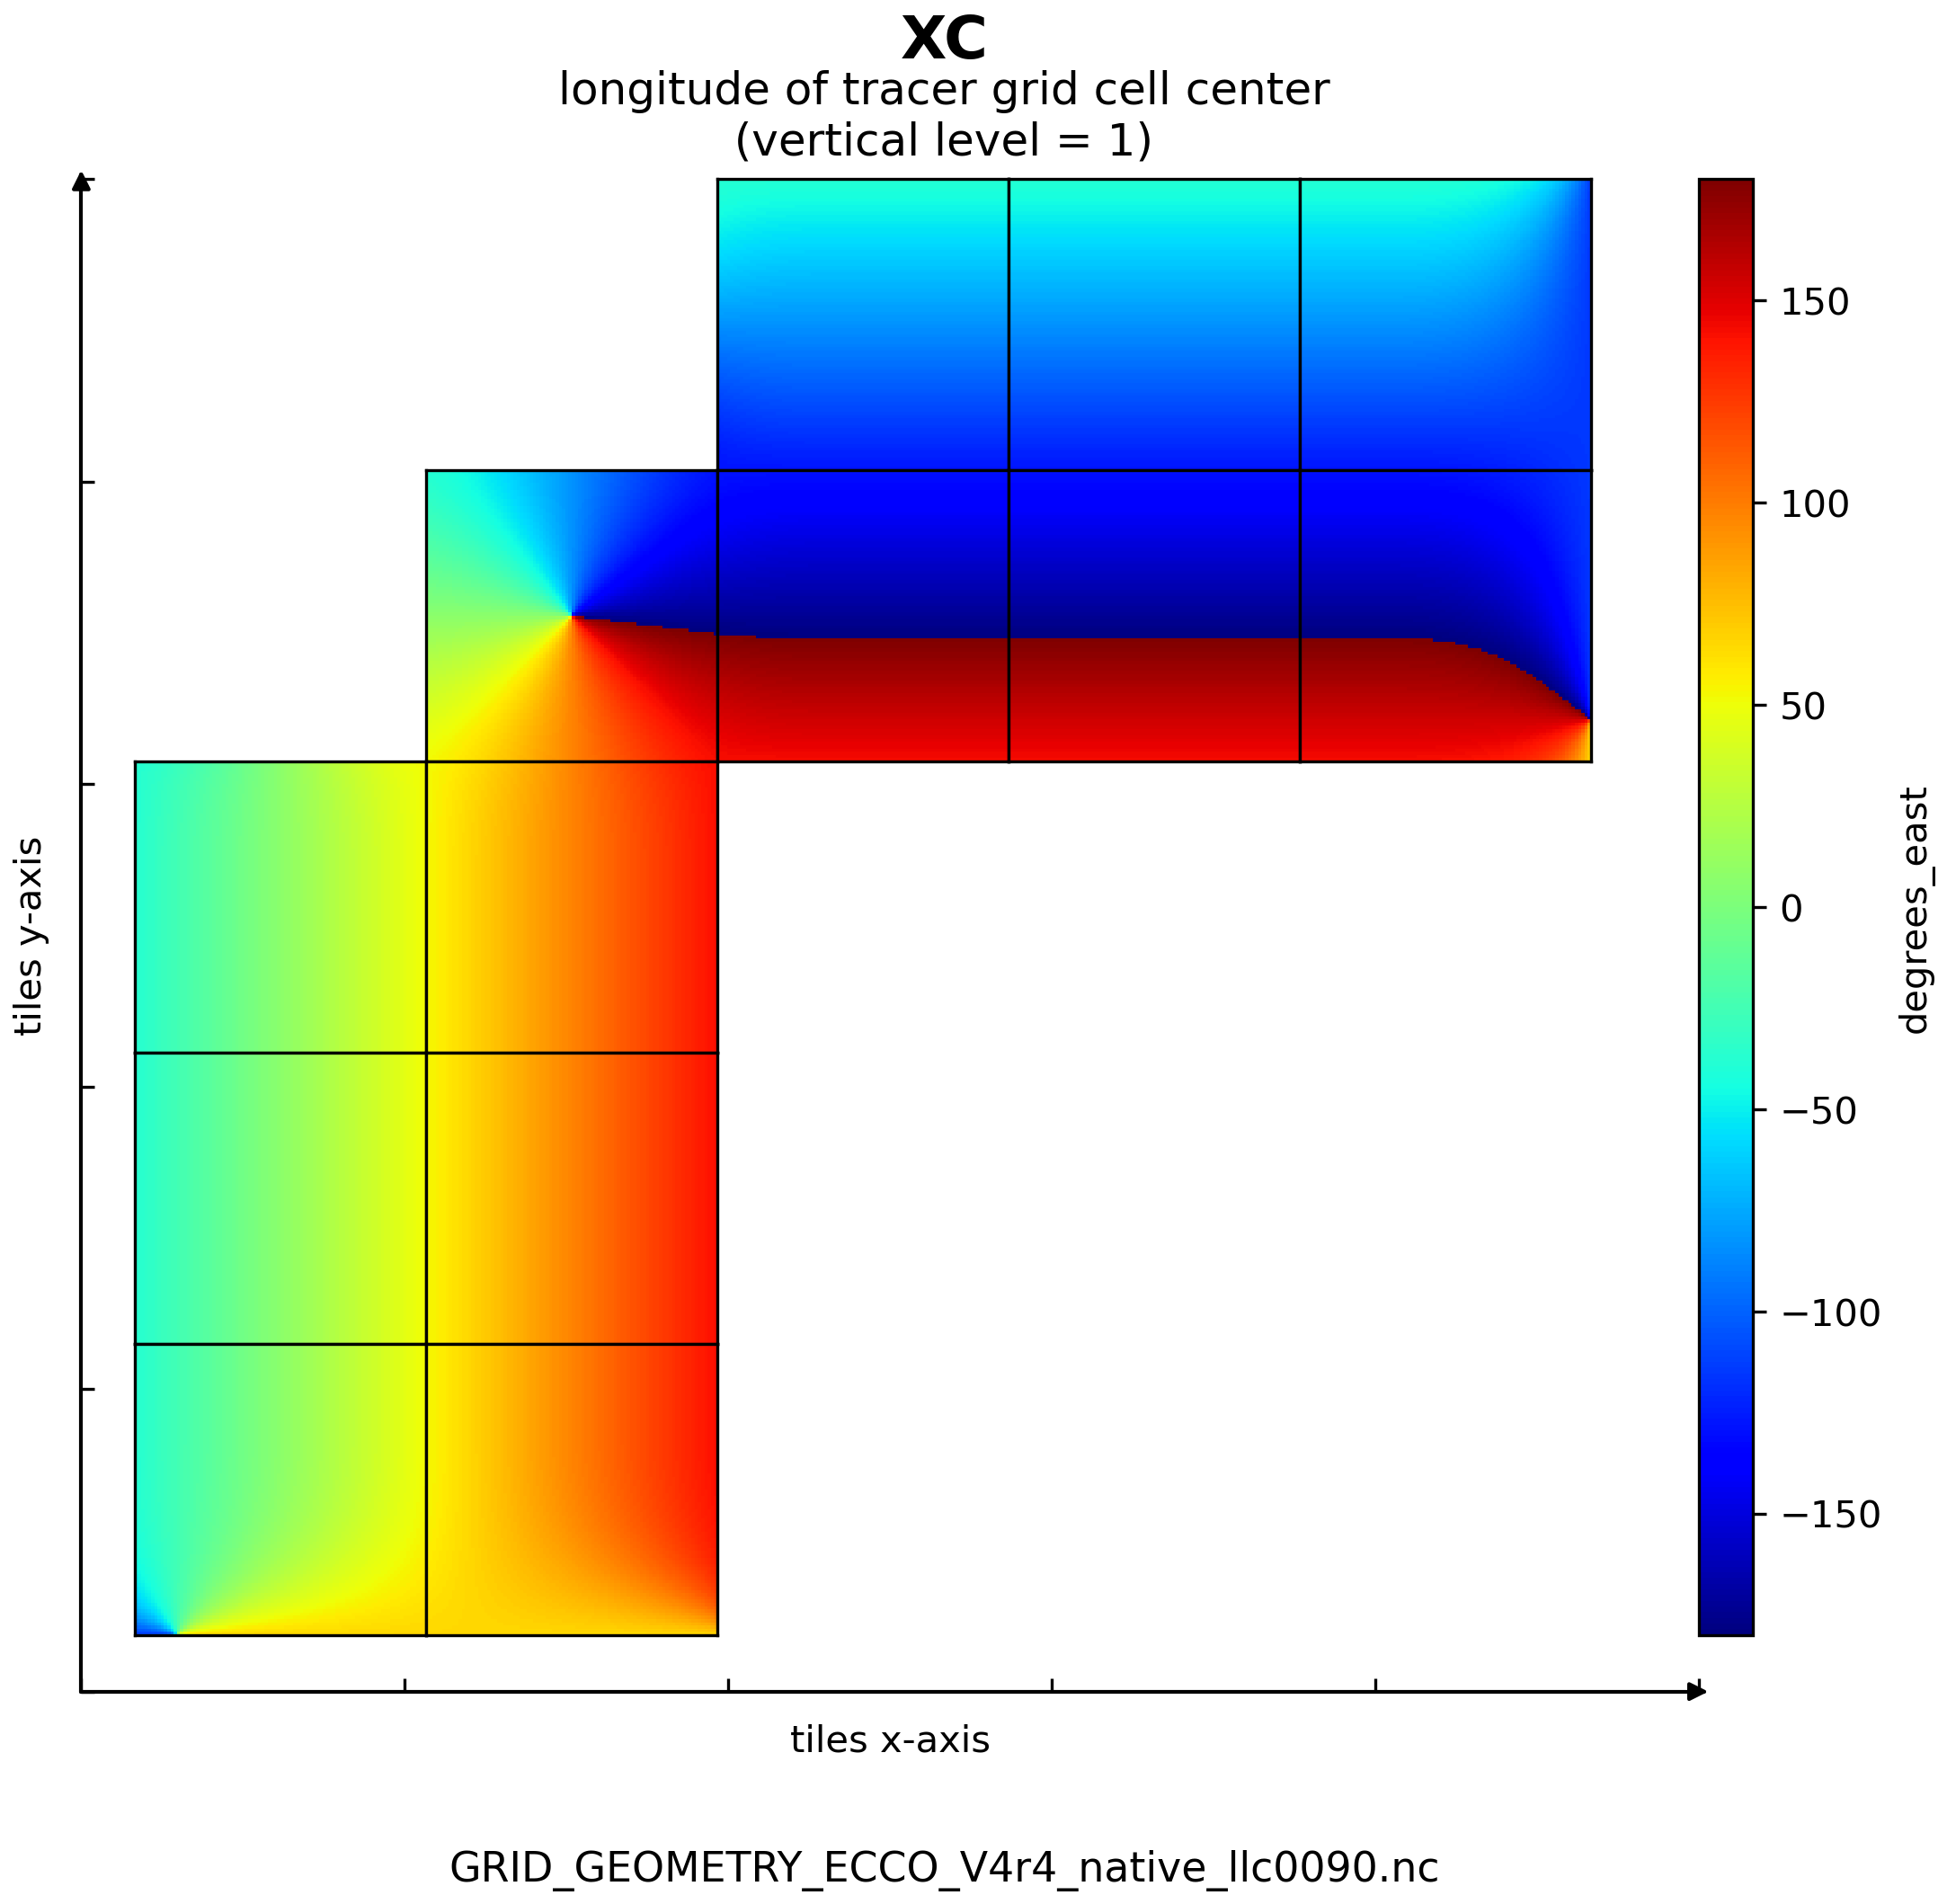
\includegraphics[scale=0.55]{../images/plots/v4r4/native_plots_coords/Geometry_Parameters_for_the_Lat-Lon-Cap_90_(llc90)_Native_Model_Grid_(Version_4_Release_4)/XC.png}
\caption{Dataset: GRID\_GEOMETRY\_ECCO, Variable: XC}
\label{tab:table-GRID_GEOMETRY_ECCO_XC-Plot}
\end{figure}
\newpage
\pagebreak
\subsubsection{Native coordinates Variable: YC}
\begin{longtable}{|m{0.06\textwidth}|m{0.3\textwidth}|m{0.45\textwidth}|m{0.12\textwidth}|}
\caption{Attributes description of the variable 'YC' from GRID\_GEOMETRY\_ECCO's  dataset.}
\label{tab:table-GRID_GEOMETRY_ECCO_YC} \\ 
\hline \endhead \hline \endfoot
\rowcolor{lightgray} \textbf{Storage Type} & \textbf{Variable Name} & \textbf{Description} & \textbf{Unit} \\ \hline
float32 & YC & Latitude of tracer grid cell center & degrees\_north \\ \hline
\multicolumn{4}{|c|}{\cellcolor{lightgray}{\textbf{Description of the variable in Common Data language (CDL)}}} \\ \hline
\multicolumn{4}{|c|}{\fontfamily{lmtt}\selectfont{\makecell{\parbox{.95\textwidth}{\vspace*{0.25cm} \footnotesize{float32 YC(tile, j, i)\\
\hspace*{0.5cm}YC: bounds =\hspace*{0.5cm} YC bnds\\
\hspace*{0.5cm}YC: coordinate =\hspace*{0.5cm} YC XC\\
\hspace*{0.5cm}YC: coverage\_content\_type = coordinate\\
\hspace*{0.5cm}YC: long\_name = latitude of tracer grid cell center\\
\hspace*{0.5cm}YC: standard\_name = latitude\\
\hspace*{0.5cm}YC: units = degrees north\\
}}}}} \\ \hline
\rowcolor{lightgray} \multicolumn{4}{|c|}{\textbf{Comments}} \\ \hline
\multicolumn{4}{|p{1\textwidth}|}{\footnotesize{{Nonuniform grid spacing}}} \\ \hline
\end{longtable}

\begin{figure}[H]
\centering
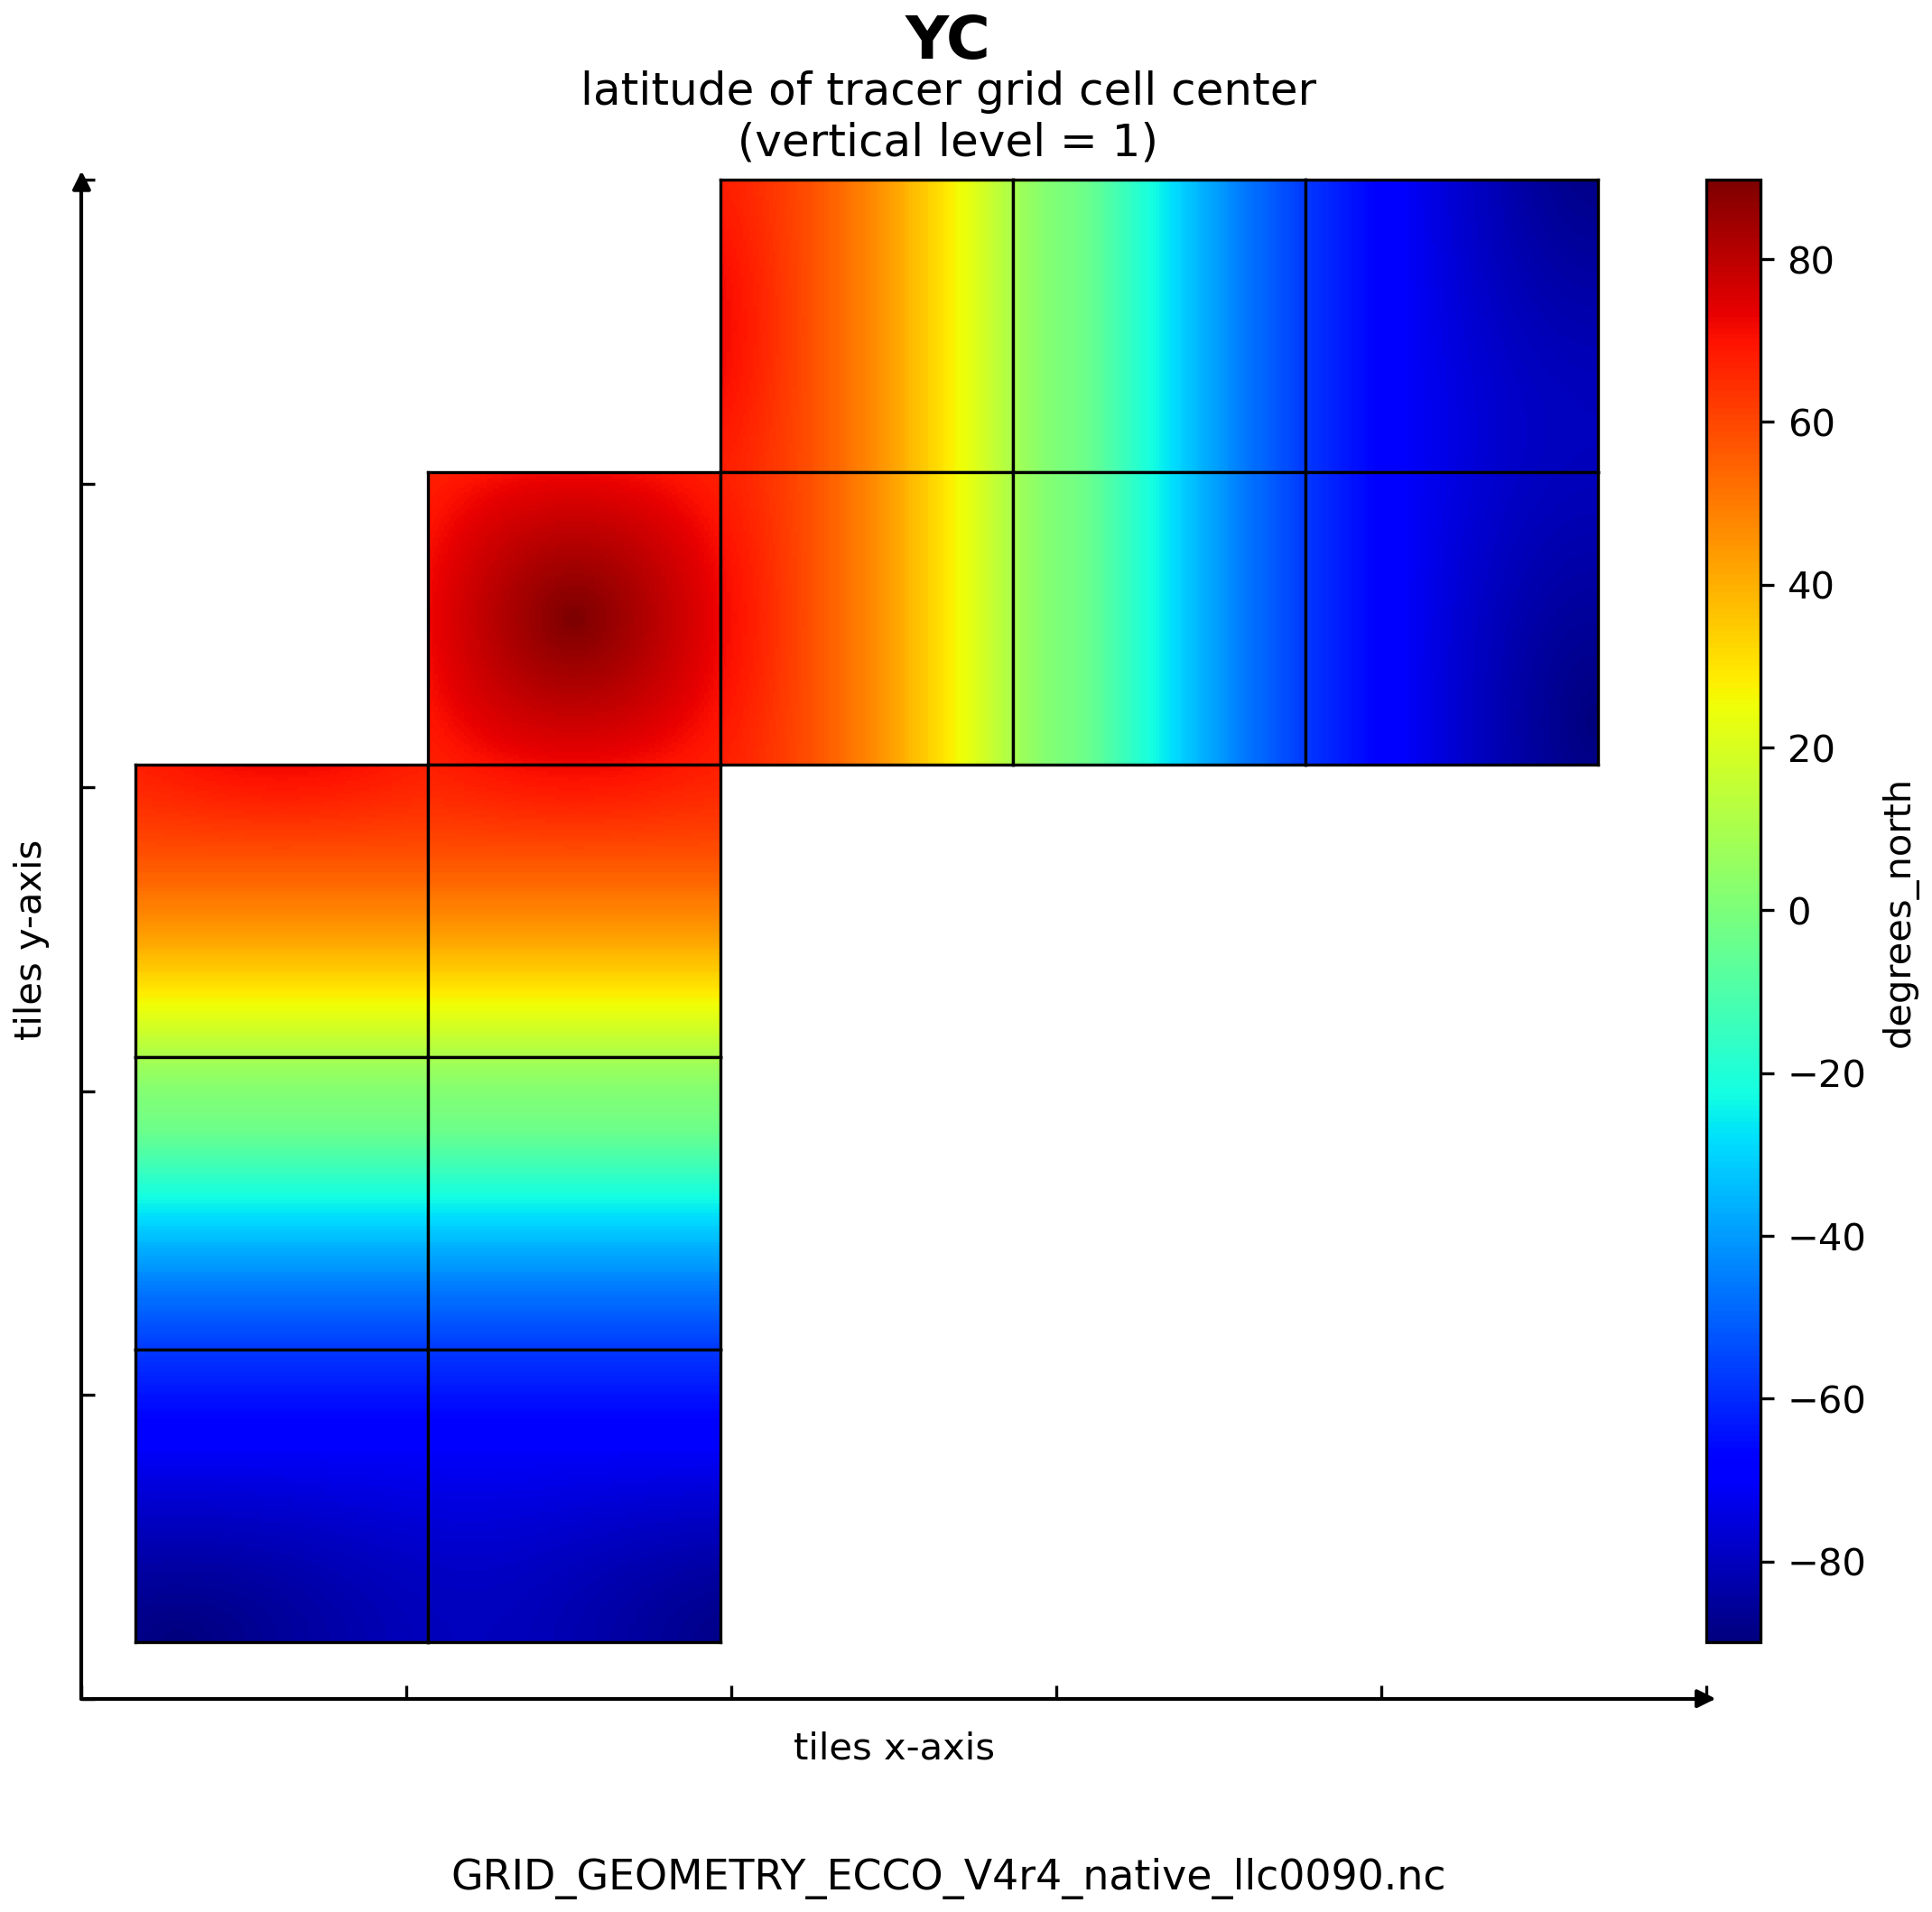
\includegraphics[scale=0.55]{../images/plots/v4r4/native_plots_coords/Geometry_Parameters_for_the_Lat-Lon-Cap_90_(llc90)_Native_Model_Grid_(Version_4_Release_4)/YC.png}
\caption{Dataset: GRID\_GEOMETRY\_ECCO, Variable: YC}
\label{tab:table-GRID_GEOMETRY_ECCO_YC-Plot}
\end{figure}
\newpage
\pagebreak
\subsubsection{Native coordinates Variable: XG}
\begin{longtable}{|m{0.06\textwidth}|m{0.3\textwidth}|m{0.45\textwidth}|m{0.12\textwidth}|}
\caption{Attributes description of the variable 'XG' from GRID\_GEOMETRY\_ECCO's  dataset.}
\label{tab:table-GRID_GEOMETRY_ECCO_XG} \\ 
\hline \endhead \hline \endfoot
\rowcolor{lightgray} \textbf{Storage Type} & \textbf{Variable Name} & \textbf{Description} & \textbf{Unit} \\ \hline
float32 & XG & Longitude of 'southwest' corner of tracer grid cell & degrees\_east \\ \hline
\multicolumn{4}{|c|}{\cellcolor{lightgray}{\textbf{Description of the variable in Common Data language (CDL)}}} \\ \hline
\multicolumn{4}{|c|}{\fontfamily{lmtt}\selectfont{\makecell{\parbox{.95\textwidth}{\vspace*{0.25cm} \footnotesize{float32 XG(tile, j\_g, i\_g)\\
\hspace*{0.5cm}XG: coordinate = YG\hspace*{0.5cm} XG\\
\hspace*{0.5cm}XG: coverage\_content\_type = coordinate\\
\hspace*{0.5cm}XG: long\_name = longitude of southwest corner of tracer grid cell\\
\hspace*{0.5cm}XG: standard\_name = longitude\\
\hspace*{0.5cm}XG: units = degrees east\\
}}}}} \\ \hline
\rowcolor{lightgray} \multicolumn{4}{|c|}{\textbf{Comments}} \\ \hline
\multicolumn{4}{|p{1\textwidth}|}{\footnotesize{{Nonuniform grid spacing. note: 'southwest' does not correspond to geographic orientation but is used for convenience to describe the computational grid. see mitgcm dcoumentation for details.}}} \\ \hline
\end{longtable}

\begin{figure}[H]
\centering
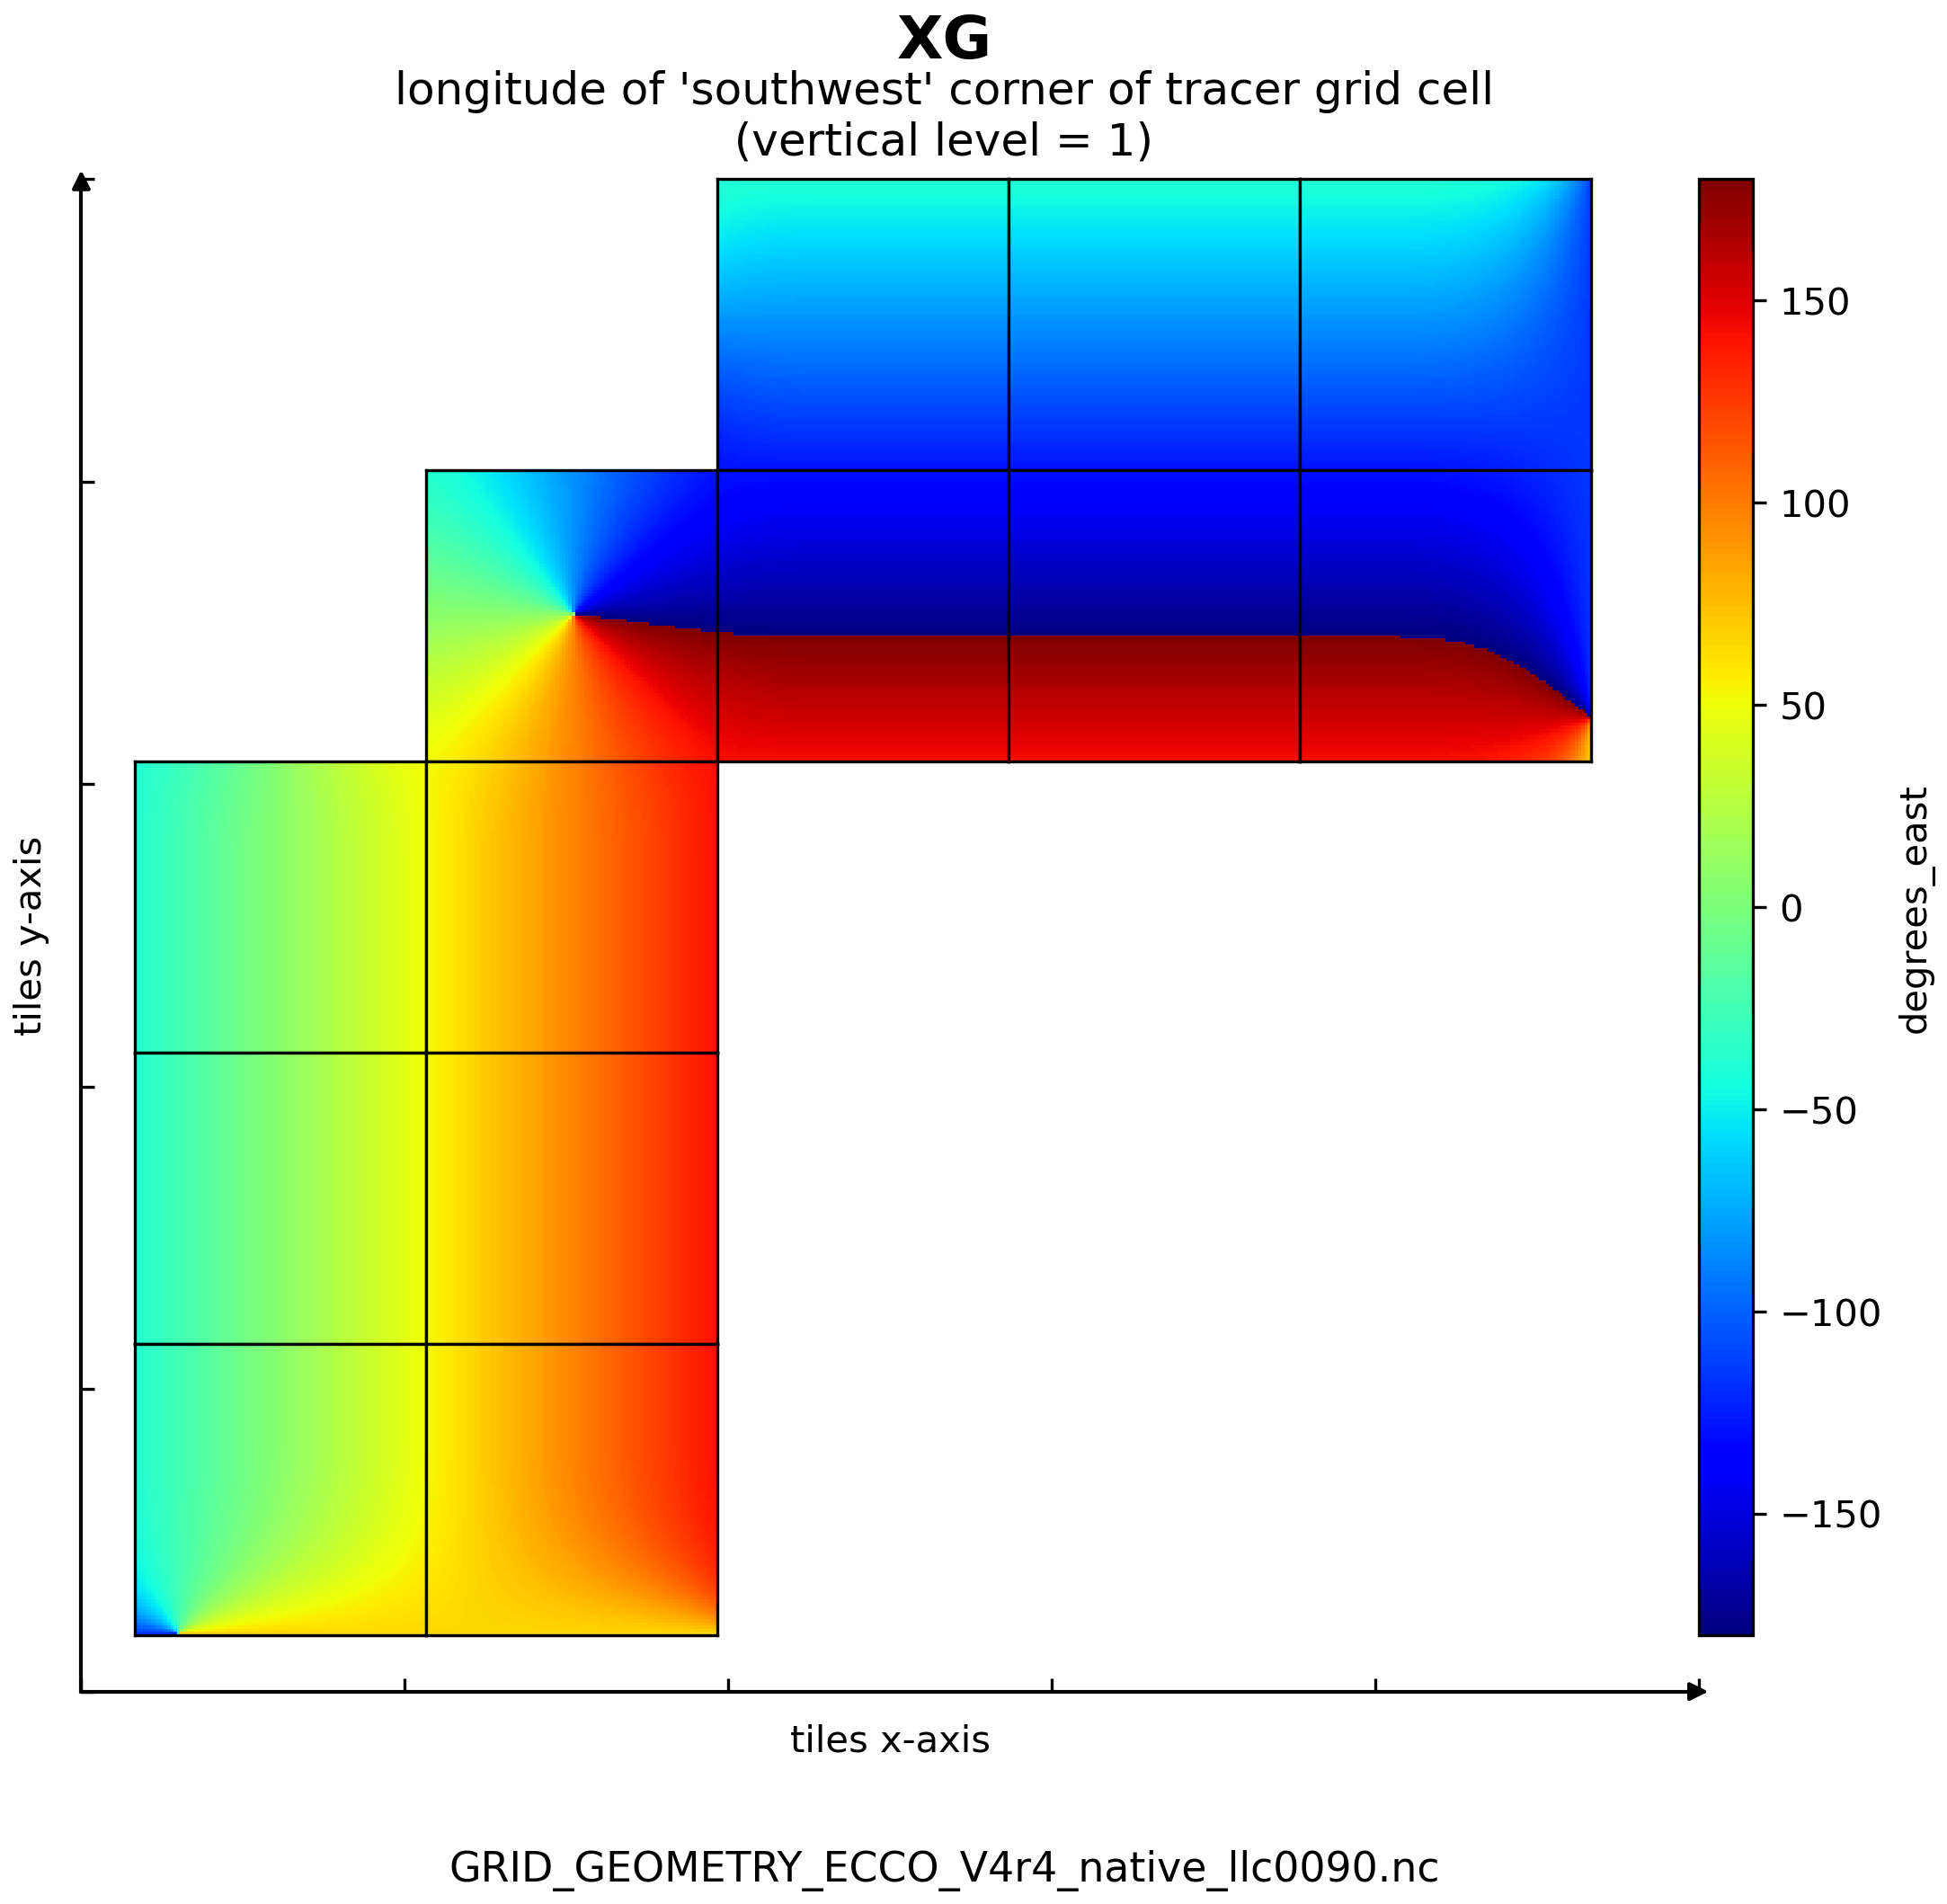
\includegraphics[scale=0.55]{../images/plots/v4r4/native_plots_coords/Geometry_Parameters_for_the_Lat-Lon-Cap_90_(llc90)_Native_Model_Grid_(Version_4_Release_4)/XG.png}
\caption{Dataset: GRID\_GEOMETRY\_ECCO, Variable: XG}
\label{tab:table-GRID_GEOMETRY_ECCO_XG-Plot}
\end{figure}
\newpage
\pagebreak
\subsubsection{Native coordinates Variable: YG}
\begin{longtable}{|m{0.06\textwidth}|m{0.3\textwidth}|m{0.45\textwidth}|m{0.12\textwidth}|}
\caption{Attributes description of the variable 'YG' from GRID\_GEOMETRY\_ECCO's  dataset.}
\label{tab:table-GRID_GEOMETRY_ECCO_YG} \\ 
\hline \endhead \hline \endfoot
\rowcolor{lightgray} \textbf{Storage Type} & \textbf{Variable Name} & \textbf{Description} & \textbf{Unit} \\ \hline
float32 & YG & Latitude of 'southwest' corner of tracer grid cell & degrees\_north \\ \hline
\multicolumn{4}{|c|}{\cellcolor{lightgray}{\textbf{Description of the variable in Common Data language (CDL)}}} \\ \hline
\multicolumn{4}{|c|}{\fontfamily{lmtt}\selectfont{\makecell{\parbox{.95\textwidth}{\vspace*{0.25cm} \footnotesize{float32 YG(tile, j\_g, i\_g)\\
\hspace*{0.5cm}YG: coordinates =\hspace*{0.5cm} YG XG\\
\hspace*{0.5cm}YG: coverage\_content\_type = coordinate\\
\hspace*{0.5cm}YG: long\_name = latitude of southwest corner of tracer grid cell\\
\hspace*{0.5cm}YG: standard\_name = latitude\\
\hspace*{0.5cm}YG: units = degrees north\\
}}}}} \\ \hline
\rowcolor{lightgray} \multicolumn{4}{|c|}{\textbf{Comments}} \\ \hline
\multicolumn{4}{|p{1\textwidth}|}{\footnotesize{{Nonuniform grid spacing. note: 'southwest' does not correspond to geographic orientation but is used for convenience to describe the computational grid. see mitgcm dcoumentation for details.}}} \\ \hline
\end{longtable}

\begin{figure}[H]
\centering
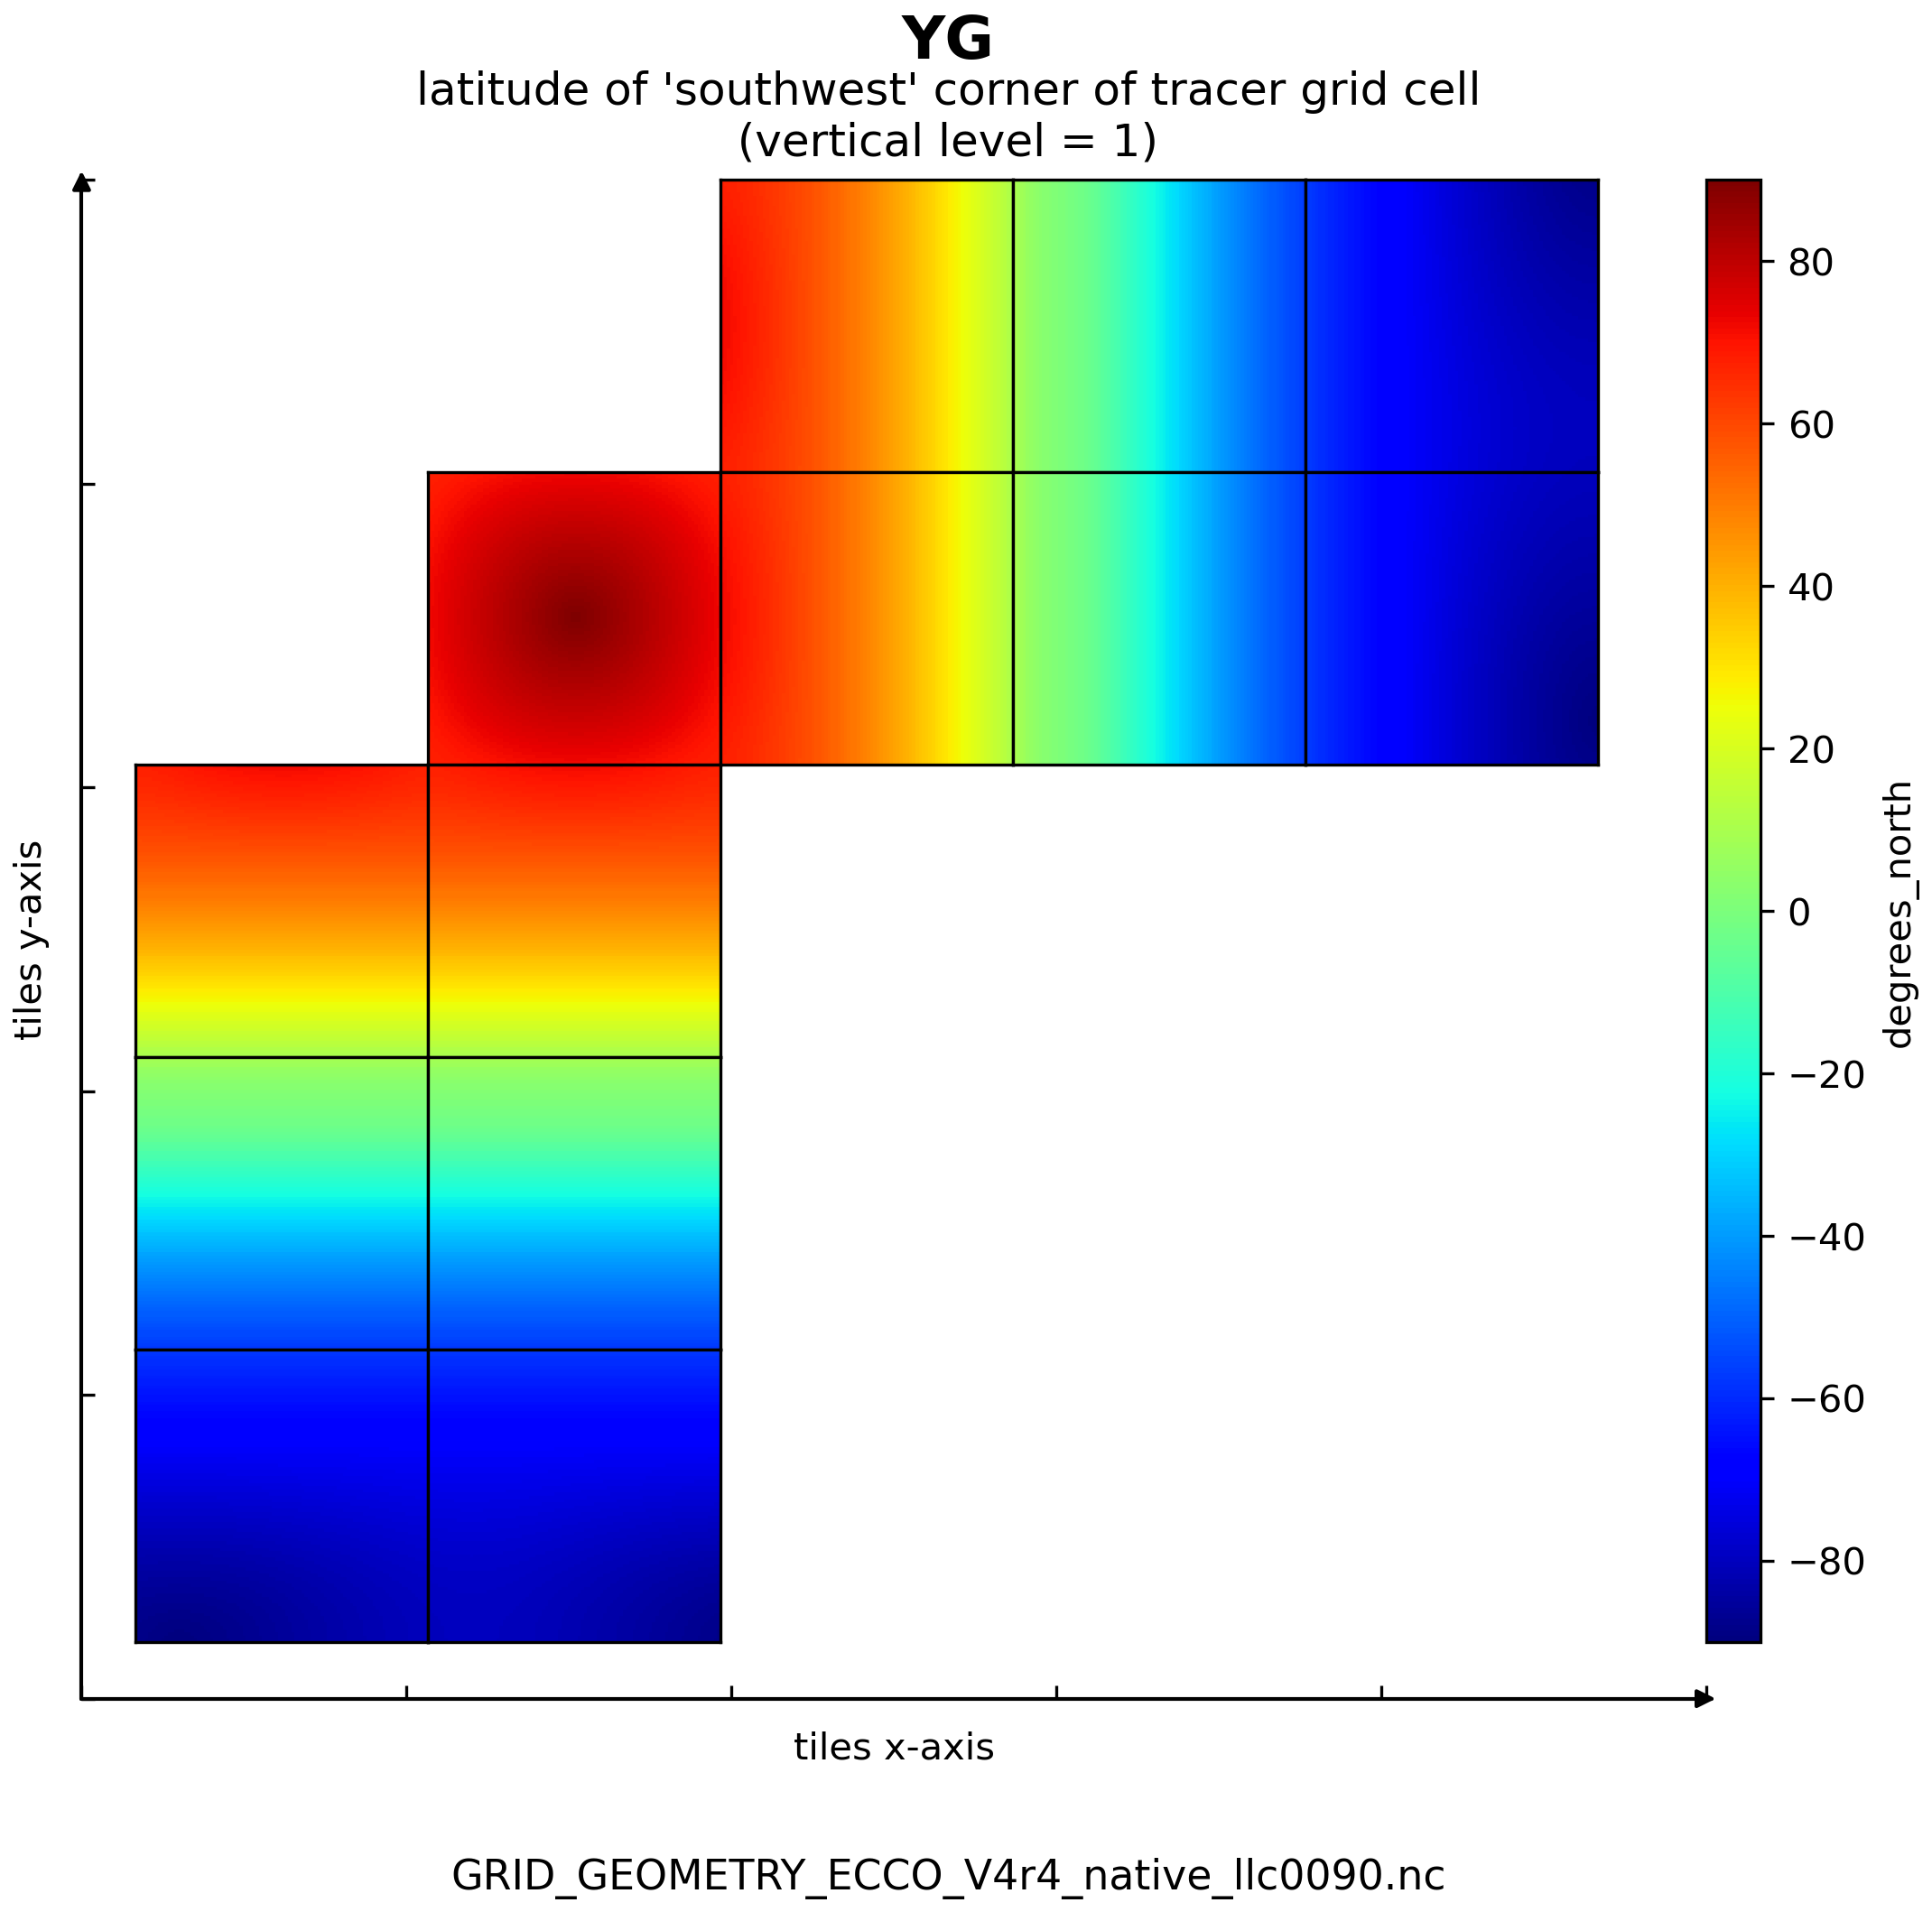
\includegraphics[scale=0.55]{../images/plots/v4r4/native_plots_coords/Geometry_Parameters_for_the_Lat-Lon-Cap_90_(llc90)_Native_Model_Grid_(Version_4_Release_4)/YG.png}
\caption{Dataset: GRID\_GEOMETRY\_ECCO, Variable: YG}
\label{tab:table-GRID_GEOMETRY_ECCO_YG-Plot}
\end{figure}
\newpage
\pagebreak
\subsubsection{Native coordinates Variable: CS}
\begin{longtable}{|m{0.06\textwidth}|m{0.3\textwidth}|m{0.45\textwidth}|m{0.12\textwidth}|}
\caption{Attributes description of the variable 'CS' from GRID\_GEOMETRY\_ECCO's  dataset.}
\label{tab:table-GRID_GEOMETRY_ECCO_CS} \\ 
\hline \endhead \hline \endfoot
\rowcolor{lightgray} \textbf{Storage Type} & \textbf{Variable Name} & \textbf{Description} & \textbf{Unit} \\ \hline
float32 & CS & Cosine of tracer grid cell orientation vs geographical north & 1 \\ \hline
\multicolumn{4}{|c|}{\cellcolor{lightgray}{\textbf{Description of the variable in Common Data language (CDL)}}} \\ \hline
\multicolumn{4}{|c|}{\fontfamily{lmtt}\selectfont{\makecell{\parbox{.95\textwidth}{\vspace*{0.25cm} \footnotesize{float32 CS(tile, j, i)\\
\hspace*{0.5cm}CS: \_FillValue = 9.96921e+36\\
\hspace*{0.5cm}CS: coordinate = YC XC\\
\hspace*{0.5cm}CS: coordinates = YC XC\\
\hspace*{0.5cm}CS: coverage\_content\_type = modelResult\\
\hspace*{0.5cm}CS: long\_name = cosine of tracer grid cell orientation vs geographical north\\
\hspace*{0.5cm}CS: units = 1\\
}}}}} \\ \hline
\rowcolor{lightgray} \multicolumn{4}{|c|}{\textbf{Comments}} \\ \hline
\multicolumn{4}{|p{1\textwidth}|}{\footnotesize{{Cs and sn are required to calculate the geographic (meridional, zonal) components of vectors on the curvilinear model grid. note: for vector r with components r\_x and r\_y: r\_\{east\} = cs r\_x - sn r\_y.  r\_\{north\} = sn r\_x + cs r\_y}}} \\ \hline
\end{longtable}

\begin{figure}[H]
\centering
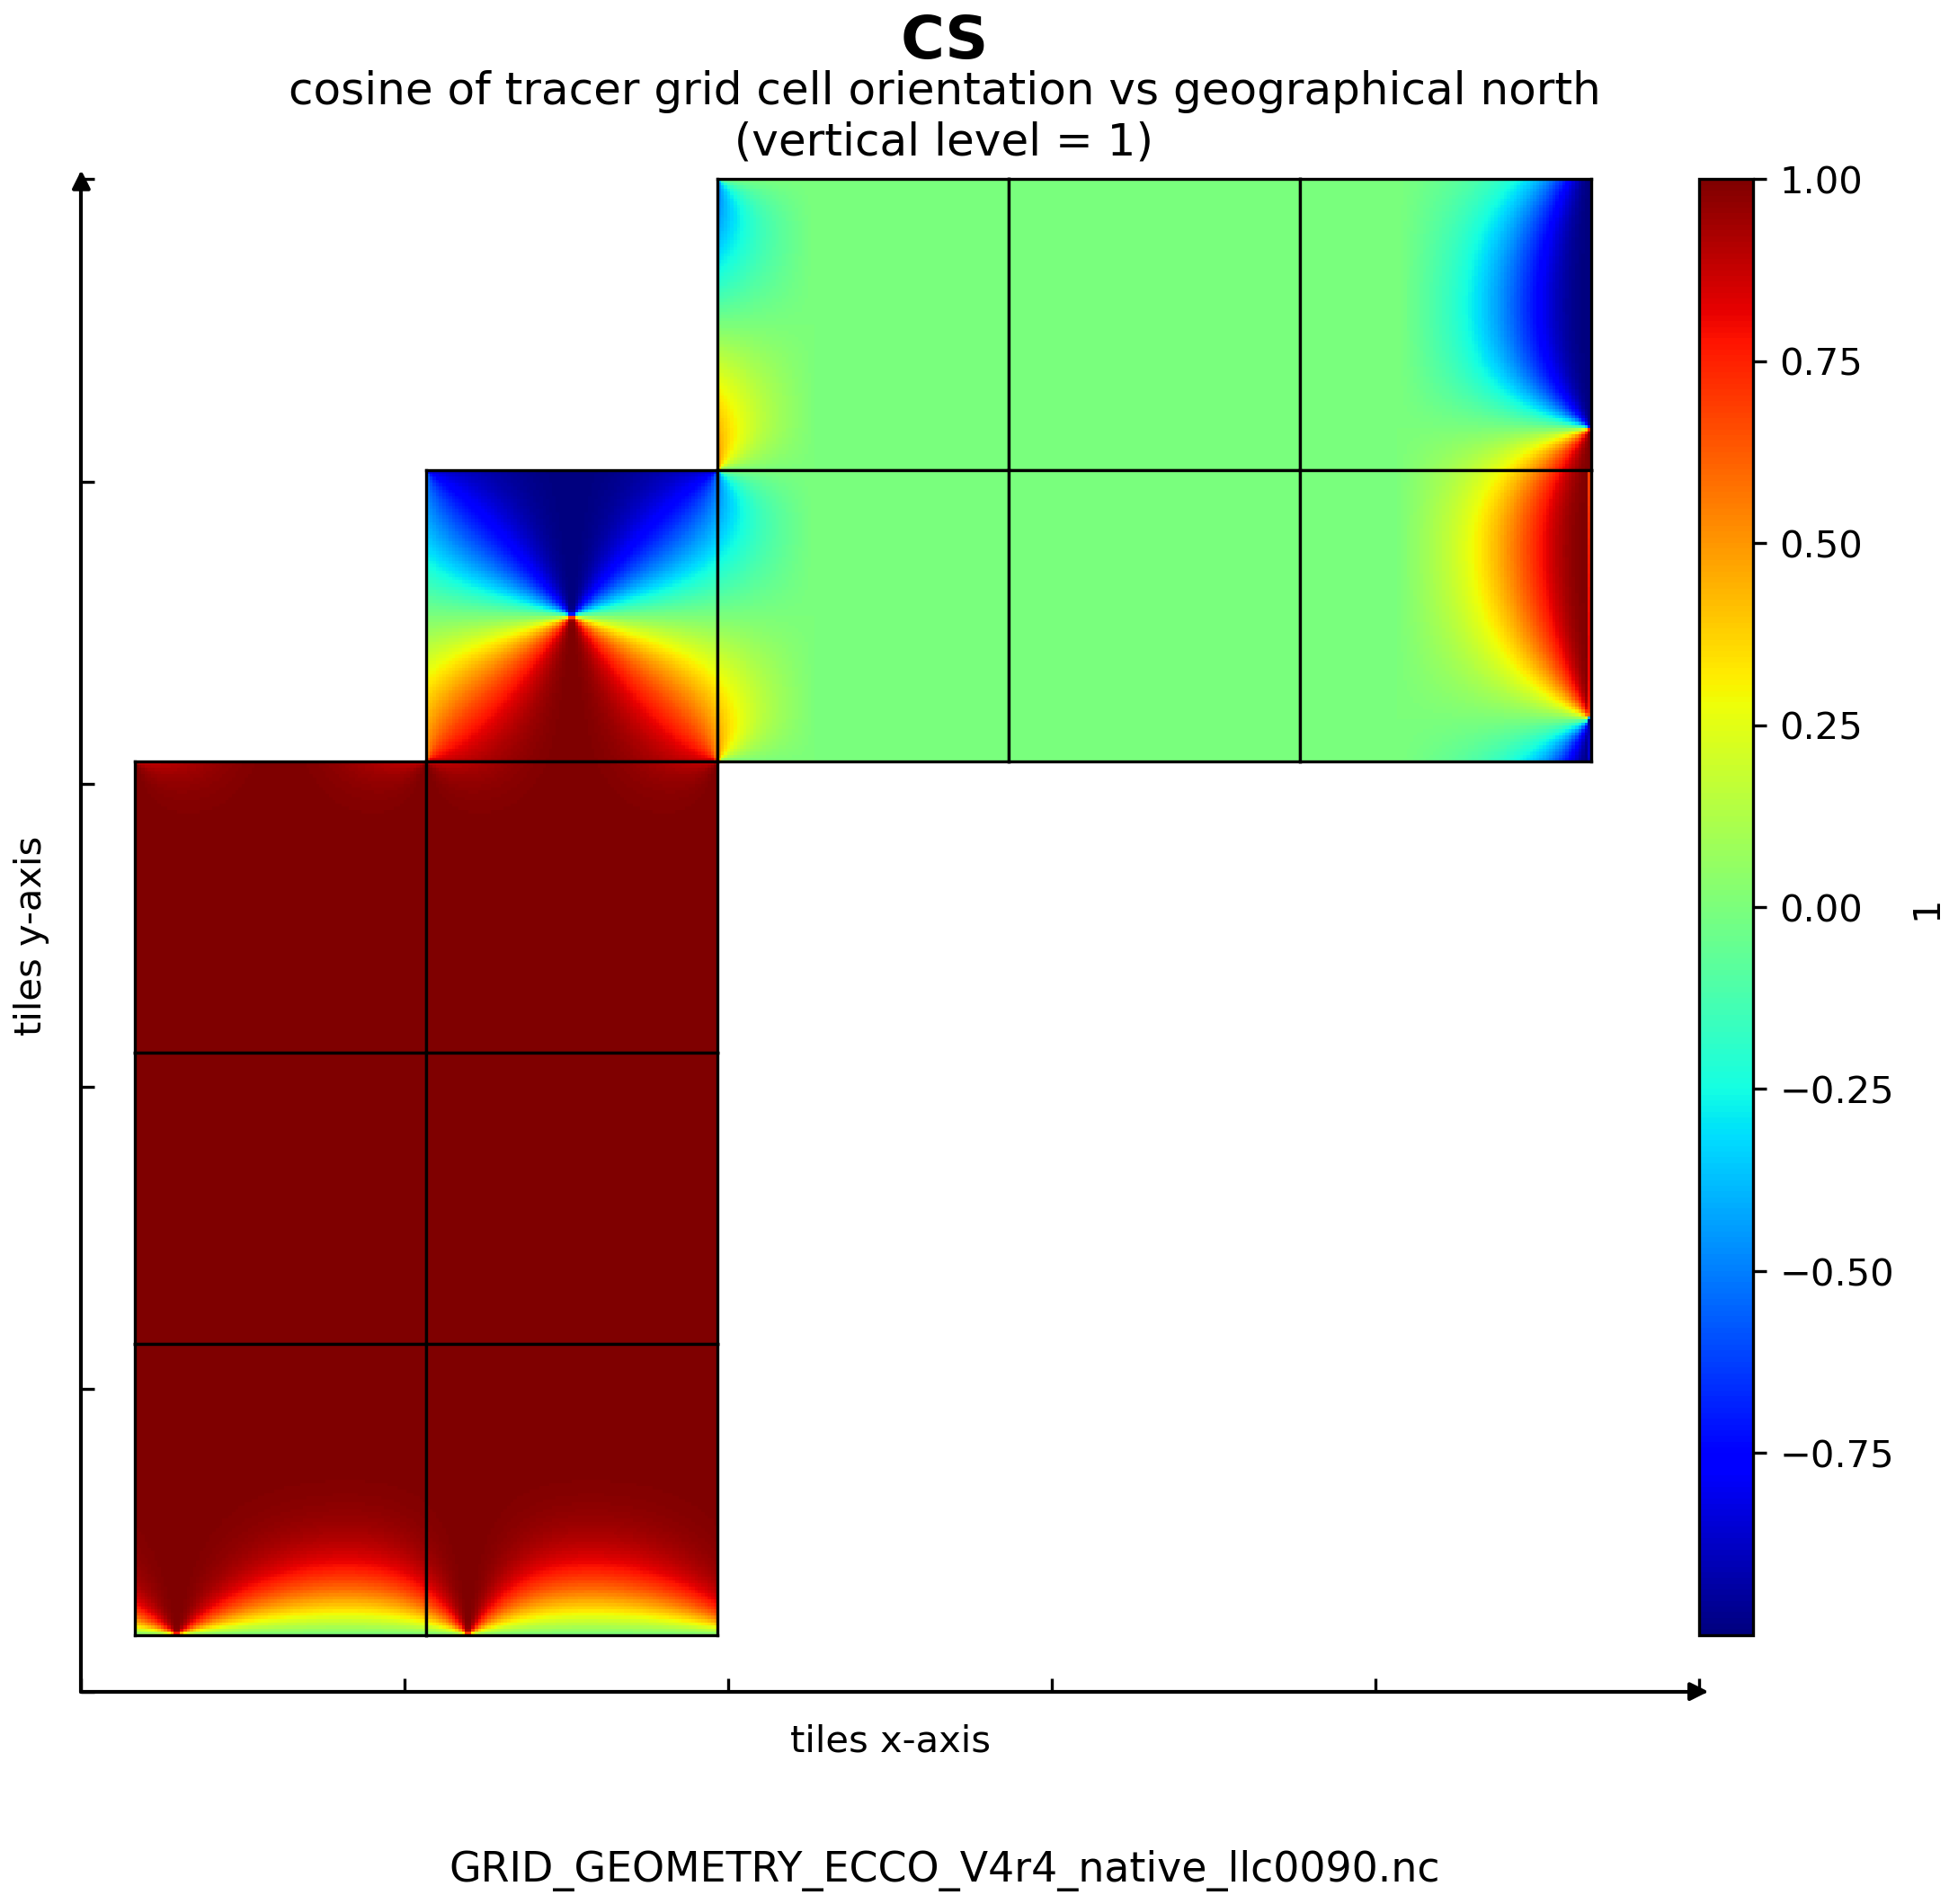
\includegraphics[scale=0.55]{../images/plots/v4r4/native_plots_coords/Geometry_Parameters_for_the_Lat-Lon-Cap_90_(llc90)_Native_Model_Grid_(Version_4_Release_4)/CS.png}
\caption{Dataset: GRID\_GEOMETRY\_ECCO, Variable: CS}
\label{tab:table-GRID_GEOMETRY_ECCO_CS-Plot}
\end{figure}
\newpage
\pagebreak
\subsubsection{Native coordinates Variable: SN}
\begin{longtable}{|m{0.06\textwidth}|m{0.3\textwidth}|m{0.45\textwidth}|m{0.12\textwidth}|}
\caption{Attributes description of the variable 'SN' from GRID\_GEOMETRY\_ECCO's  dataset.}
\label{tab:table-GRID_GEOMETRY_ECCO_SN} \\ 
\hline \endhead \hline \endfoot
\rowcolor{lightgray} \textbf{Storage Type} & \textbf{Variable Name} & \textbf{Description} & \textbf{Unit} \\ \hline
float32 & SN & Sine of tracer grid cell orientation vs geographical north & 1 \\ \hline
\multicolumn{4}{|c|}{\cellcolor{lightgray}{\textbf{Description of the variable in Common Data language (CDL)}}} \\ \hline
\multicolumn{4}{|c|}{\fontfamily{lmtt}\selectfont{\makecell{\parbox{.95\textwidth}{\vspace*{0.25cm} \footnotesize{float32 SN(tile, j, i)\\
\hspace*{0.5cm}SN: \_FillValue = 9.96921e+36\\
\hspace*{0.5cm}SN: coordinate = YC XC\\
\hspace*{0.5cm}SN: coordinates = YC XC\\
\hspace*{0.5cm}SN: coverage\_content\_type = modelResult\\
\hspace*{0.5cm}SN: long\_name = sine of tracer grid cell orientation vs geographical north\\
\hspace*{0.5cm}SN: units = 1\\
}}}}} \\ \hline
\rowcolor{lightgray} \multicolumn{4}{|c|}{\textbf{Comments}} \\ \hline
\multicolumn{4}{|p{1\textwidth}|}{\footnotesize{{Cs and sn are required to calculate the geographic (meridional, zonal) components of vectors on the curvilinear model grid. note: for vector r with components r\_x and r\_y in local grid directions x and y, the geographical eastward component r\_\{east\} = cs r\_x - sn r\_y. the geographical northward component r\_\{north\} = sn r\_x + cs r\_y.}}} \\ \hline
\end{longtable}

\begin{figure}[H]
\centering
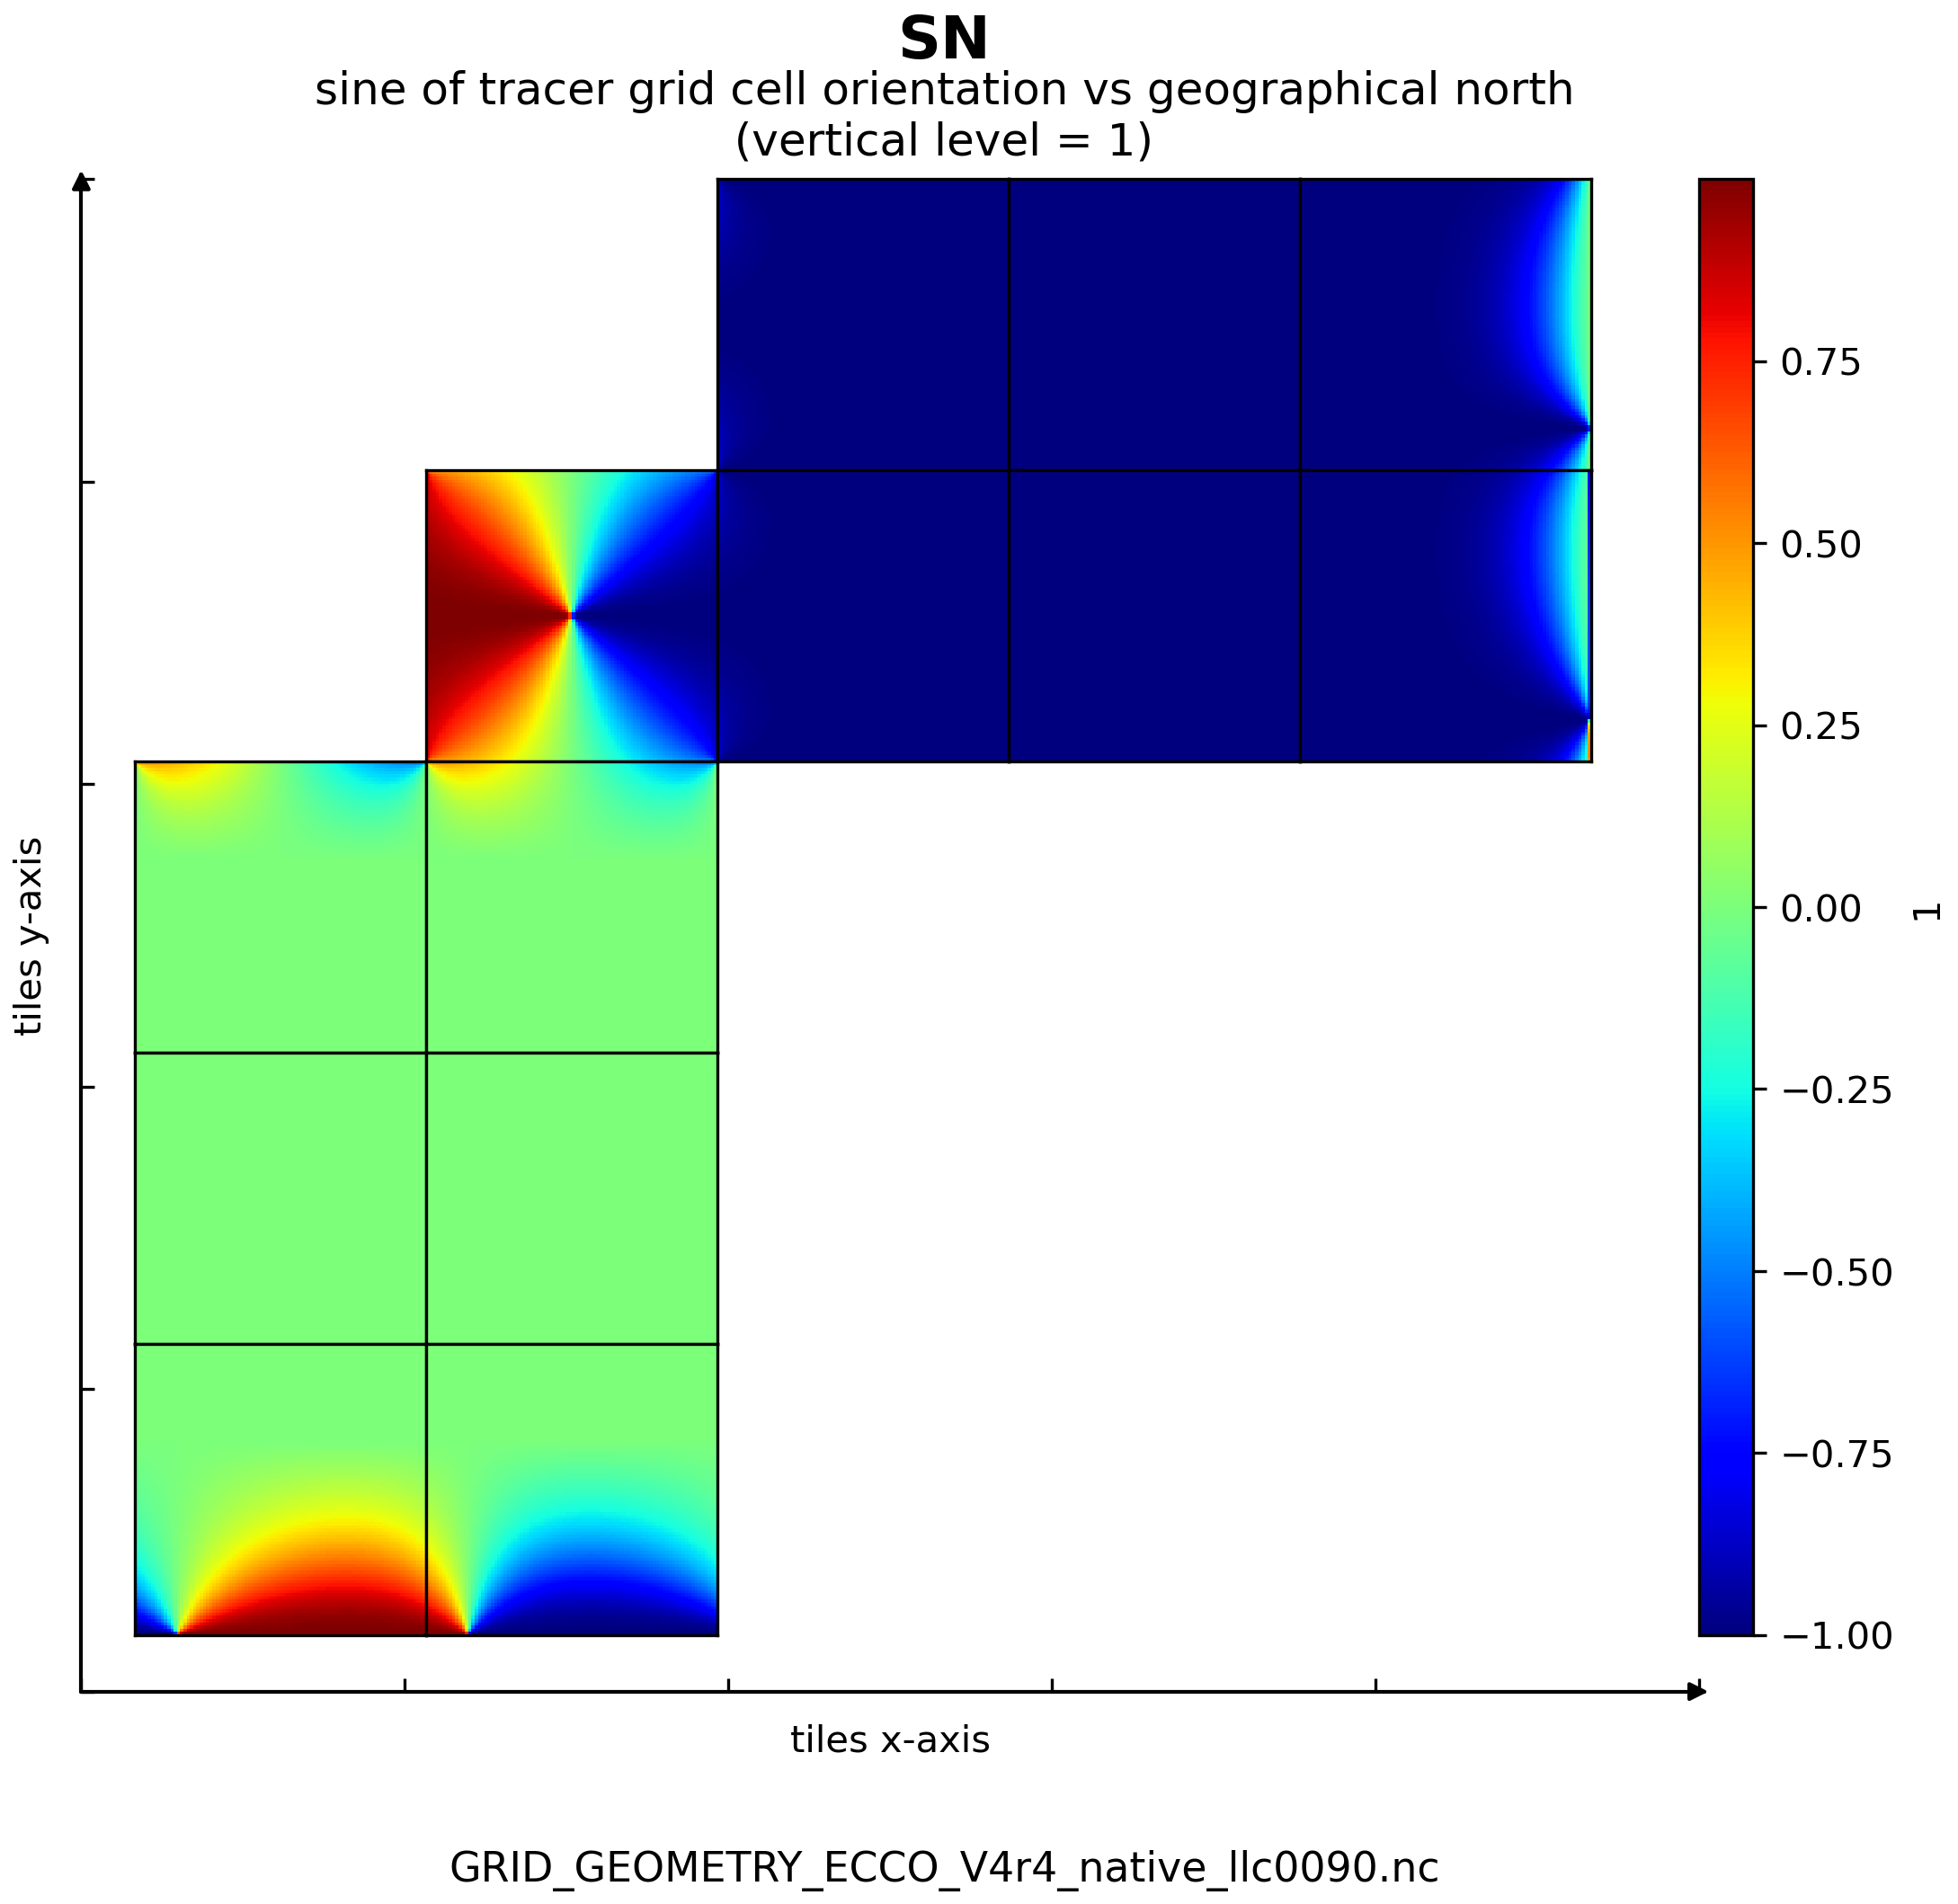
\includegraphics[scale=0.55]{../images/plots/v4r4/native_plots_coords/Geometry_Parameters_for_the_Lat-Lon-Cap_90_(llc90)_Native_Model_Grid_(Version_4_Release_4)/SN.png}
\caption{Dataset: GRID\_GEOMETRY\_ECCO, Variable: SN}
\label{tab:table-GRID_GEOMETRY_ECCO_SN-Plot}
\end{figure}
\newpage
\pagebreak
\subsubsection{Native coordinates Variable: rA}
\begin{longtable}{|m{0.06\textwidth}|m{0.3\textwidth}|m{0.45\textwidth}|m{0.12\textwidth}|}
\caption{Attributes description of the variable 'rA' from GRID\_GEOMETRY\_ECCO's  dataset.}
\label{tab:table-GRID_GEOMETRY_ECCO_rA} \\ 
\hline \endhead \hline \endfoot
\rowcolor{lightgray} \textbf{Storage Type} & \textbf{Variable Name} & \textbf{Description} & \textbf{Unit} \\ \hline
float32 & rA & Area of tracer grid cell & m2 \\ \hline
\multicolumn{4}{|c|}{\cellcolor{lightgray}{\textbf{Description of the variable in Common Data language (CDL)}}} \\ \hline
\multicolumn{4}{|c|}{\fontfamily{lmtt}\selectfont{\makecell{\parbox{.95\textwidth}{\vspace*{0.25cm} \footnotesize{float32 rA(tile, j, i)\\
\hspace*{0.5cm}rA: \_FillValue = 9.96921e+36\\
\hspace*{0.5cm}rA: coordinate = YC XC\\
\hspace*{0.5cm}rA: coordinates = YC XC\\
\hspace*{0.5cm}rA: coverage\_content\_type = modelResult\\
\hspace*{0.5cm}rA: long\_name = area of tracer grid cell\\
\hspace*{0.5cm}rA: standard\_name = cell area\\
\hspace*{0.5cm}rA: units = m2\\
}}}}} \\ \hline
\rowcolor{lightgray} \multicolumn{4}{|c|}{\textbf{Comments}} \\ \hline
\multicolumn{4}{|p{1\textwidth}|}{\footnotesize{{N/a}}} \\ \hline
\end{longtable}

\begin{figure}[H]
\centering
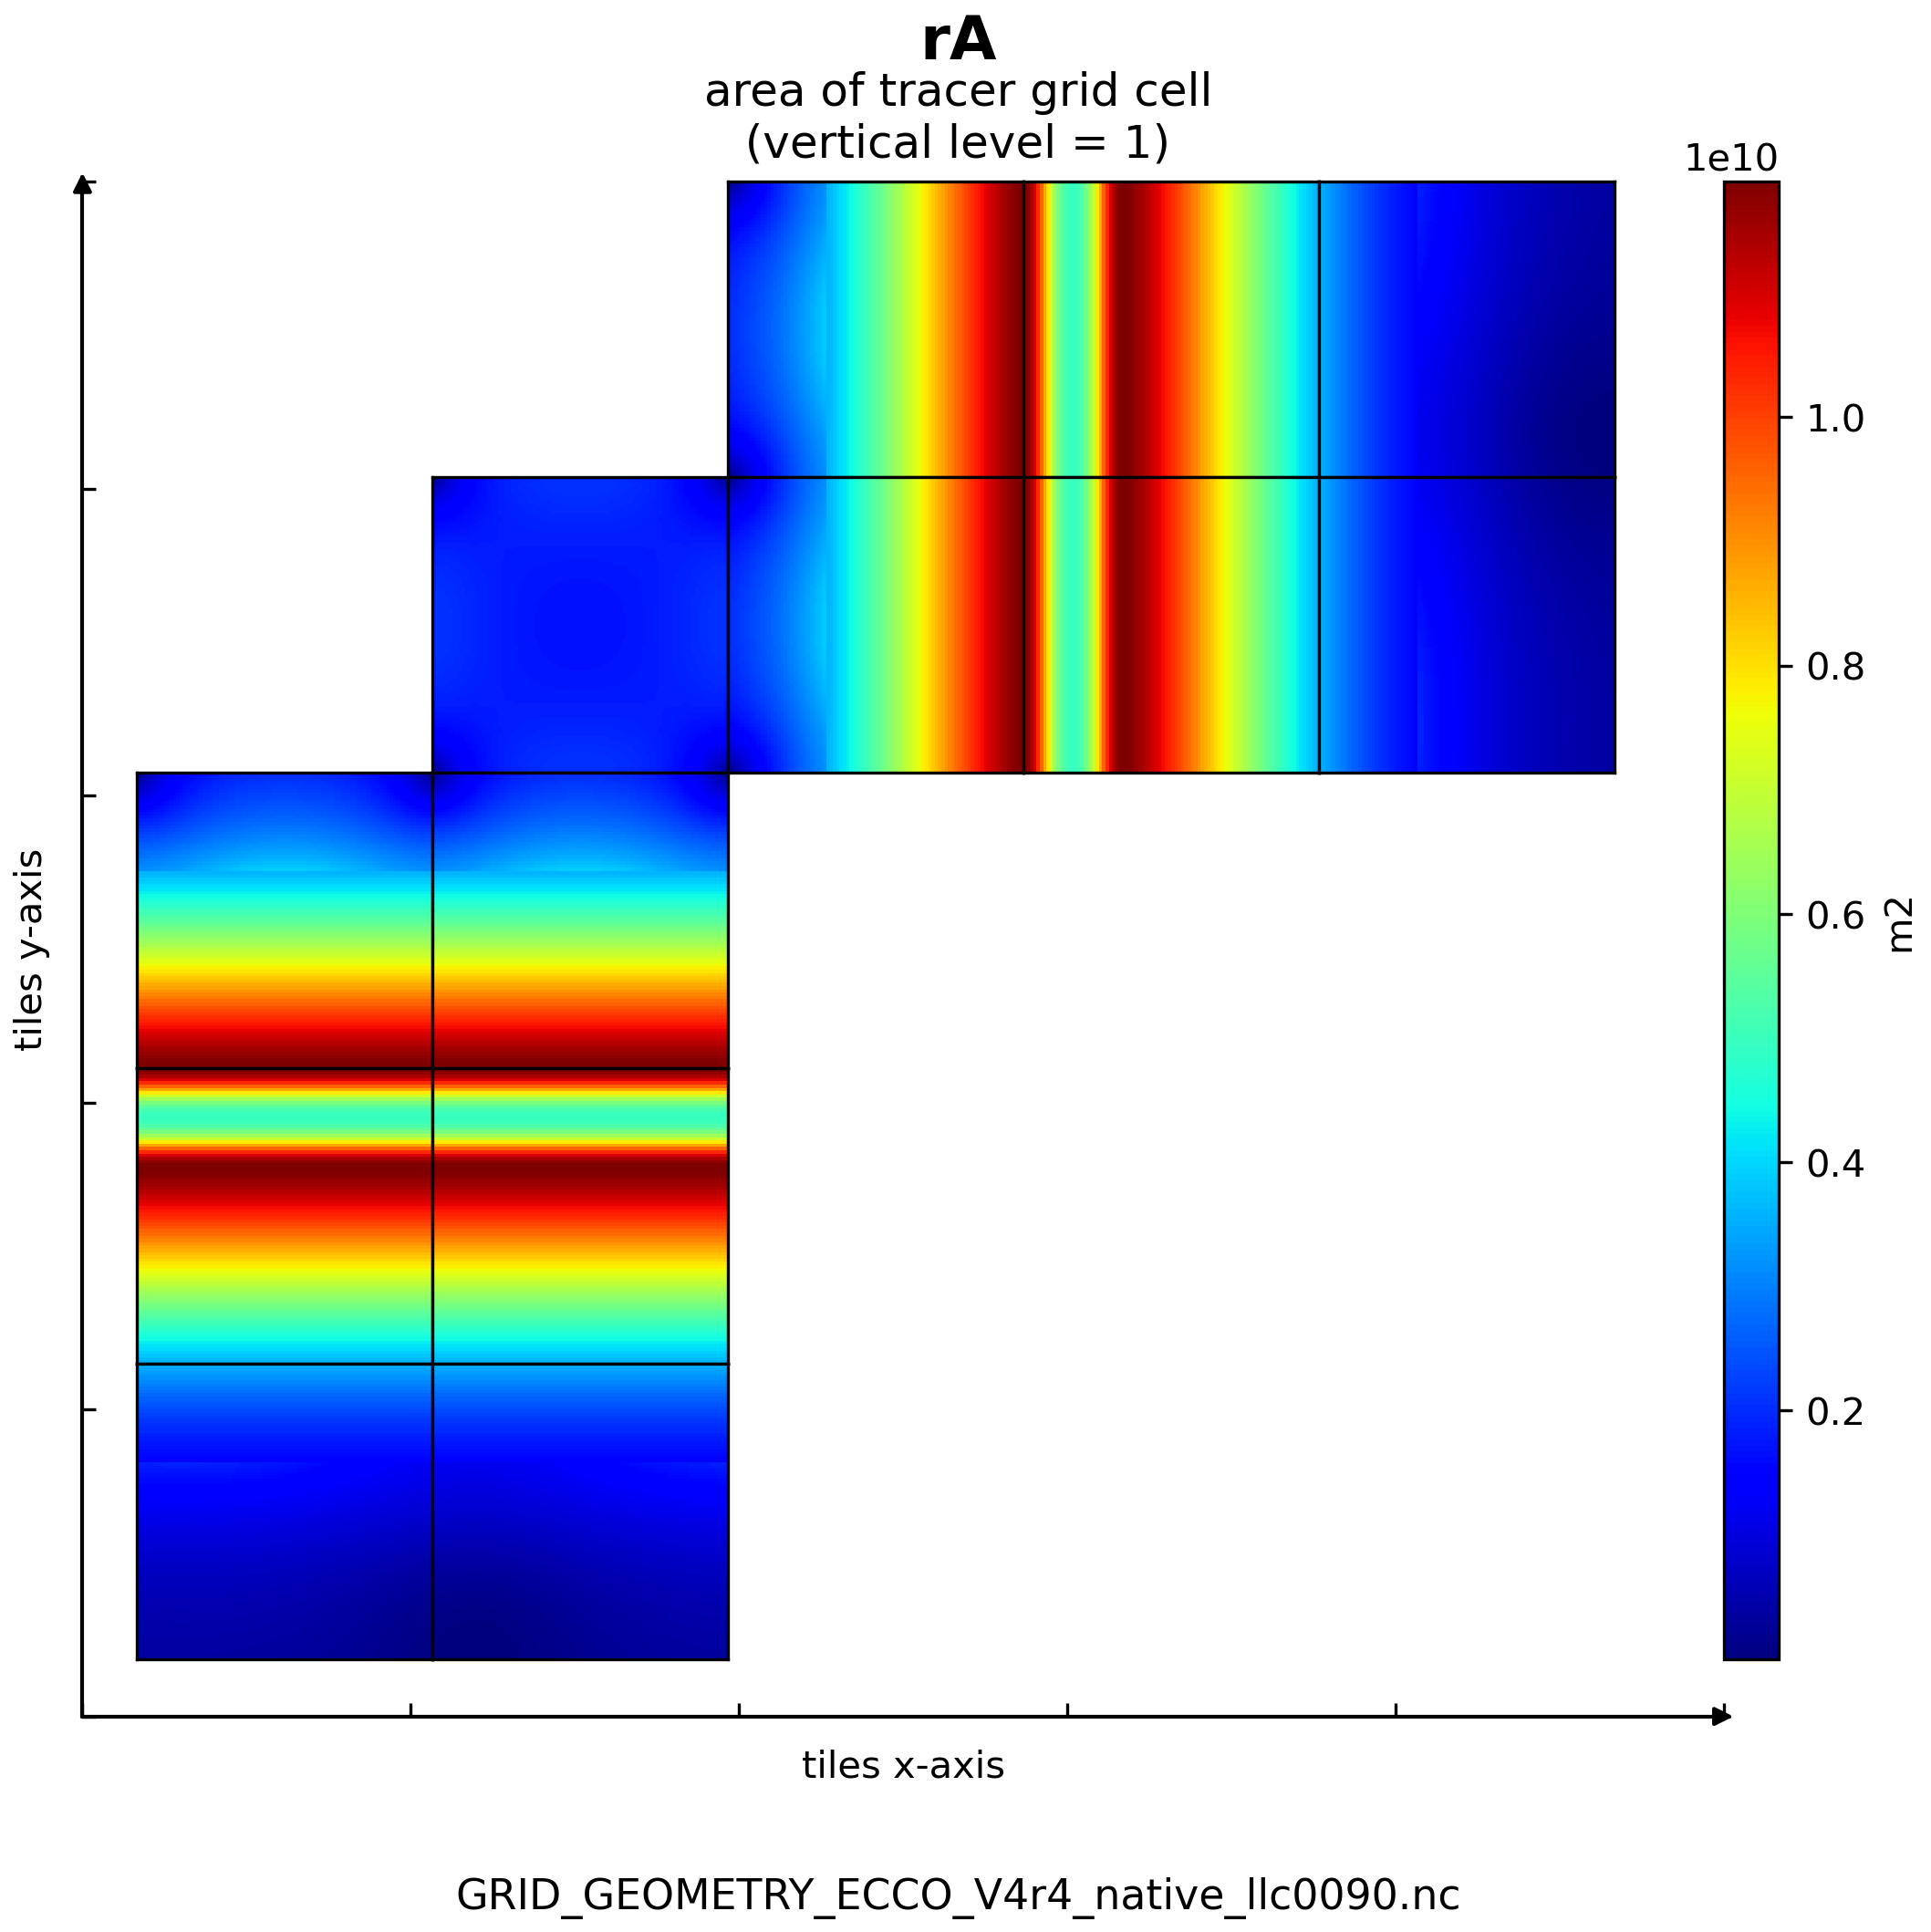
\includegraphics[scale=0.55]{../images/plots/v4r4/native_plots_coords/Geometry_Parameters_for_the_Lat-Lon-Cap_90_(llc90)_Native_Model_Grid_(Version_4_Release_4)/rA.png}
\caption{Dataset: GRID\_GEOMETRY\_ECCO, Variable: rA}
\label{tab:table-GRID_GEOMETRY_ECCO_rA-Plot}
\end{figure}
\newpage
\pagebreak
\subsubsection{Native coordinates Variable: dxG}
\begin{longtable}{|m{0.06\textwidth}|m{0.3\textwidth}|m{0.45\textwidth}|m{0.12\textwidth}|}
\caption{Attributes description of the variable 'dxG' from GRID\_GEOMETRY\_ECCO's  dataset.}
\label{tab:table-GRID_GEOMETRY_ECCO_dxG} \\ 
\hline \endhead \hline \endfoot
\rowcolor{lightgray} \textbf{Storage Type} & \textbf{Variable Name} & \textbf{Description} & \textbf{Unit} \\ \hline
float32 & dxG & Distance between 'southwest' and 'southeast' corners of the tracer grid cell & m \\ \hline
\multicolumn{4}{|c|}{\cellcolor{lightgray}{\textbf{Description of the variable in Common Data language (CDL)}}} \\ \hline
\multicolumn{4}{|c|}{\fontfamily{lmtt}\selectfont{\makecell{\parbox{.95\textwidth}{\vspace*{0.25cm} \footnotesize{float32 dxG(tile, j\_g, i)\\
\hspace*{0.5cm}dxG: \_FillValue = 9.96921e+36\\
\hspace*{0.5cm}dxG: coordinate = YG XC\\
\hspace*{0.5cm}dxG: coverage\_content\_type = modelResult\\
\hspace*{0.5cm}dxG: long\_name = distance between southwest and southeast corners of the tracer grid cell\\
\hspace*{0.5cm}dxG: units = m\\
}}}}} \\ \hline
\rowcolor{lightgray} \multicolumn{4}{|c|}{\textbf{Comments}} \\ \hline
\multicolumn{4}{|p{1\textwidth}|}{\footnotesize{{Alternatively, the length of 'south' side of tracer grid cell. note: 'south', 'southwest', and 'southeast' do not correspond to geographic orientation but are used for convenience to describe the computational grid. see mitgcm documentation for details.}}} \\ \hline
\end{longtable}

\begin{figure}[H]
\centering
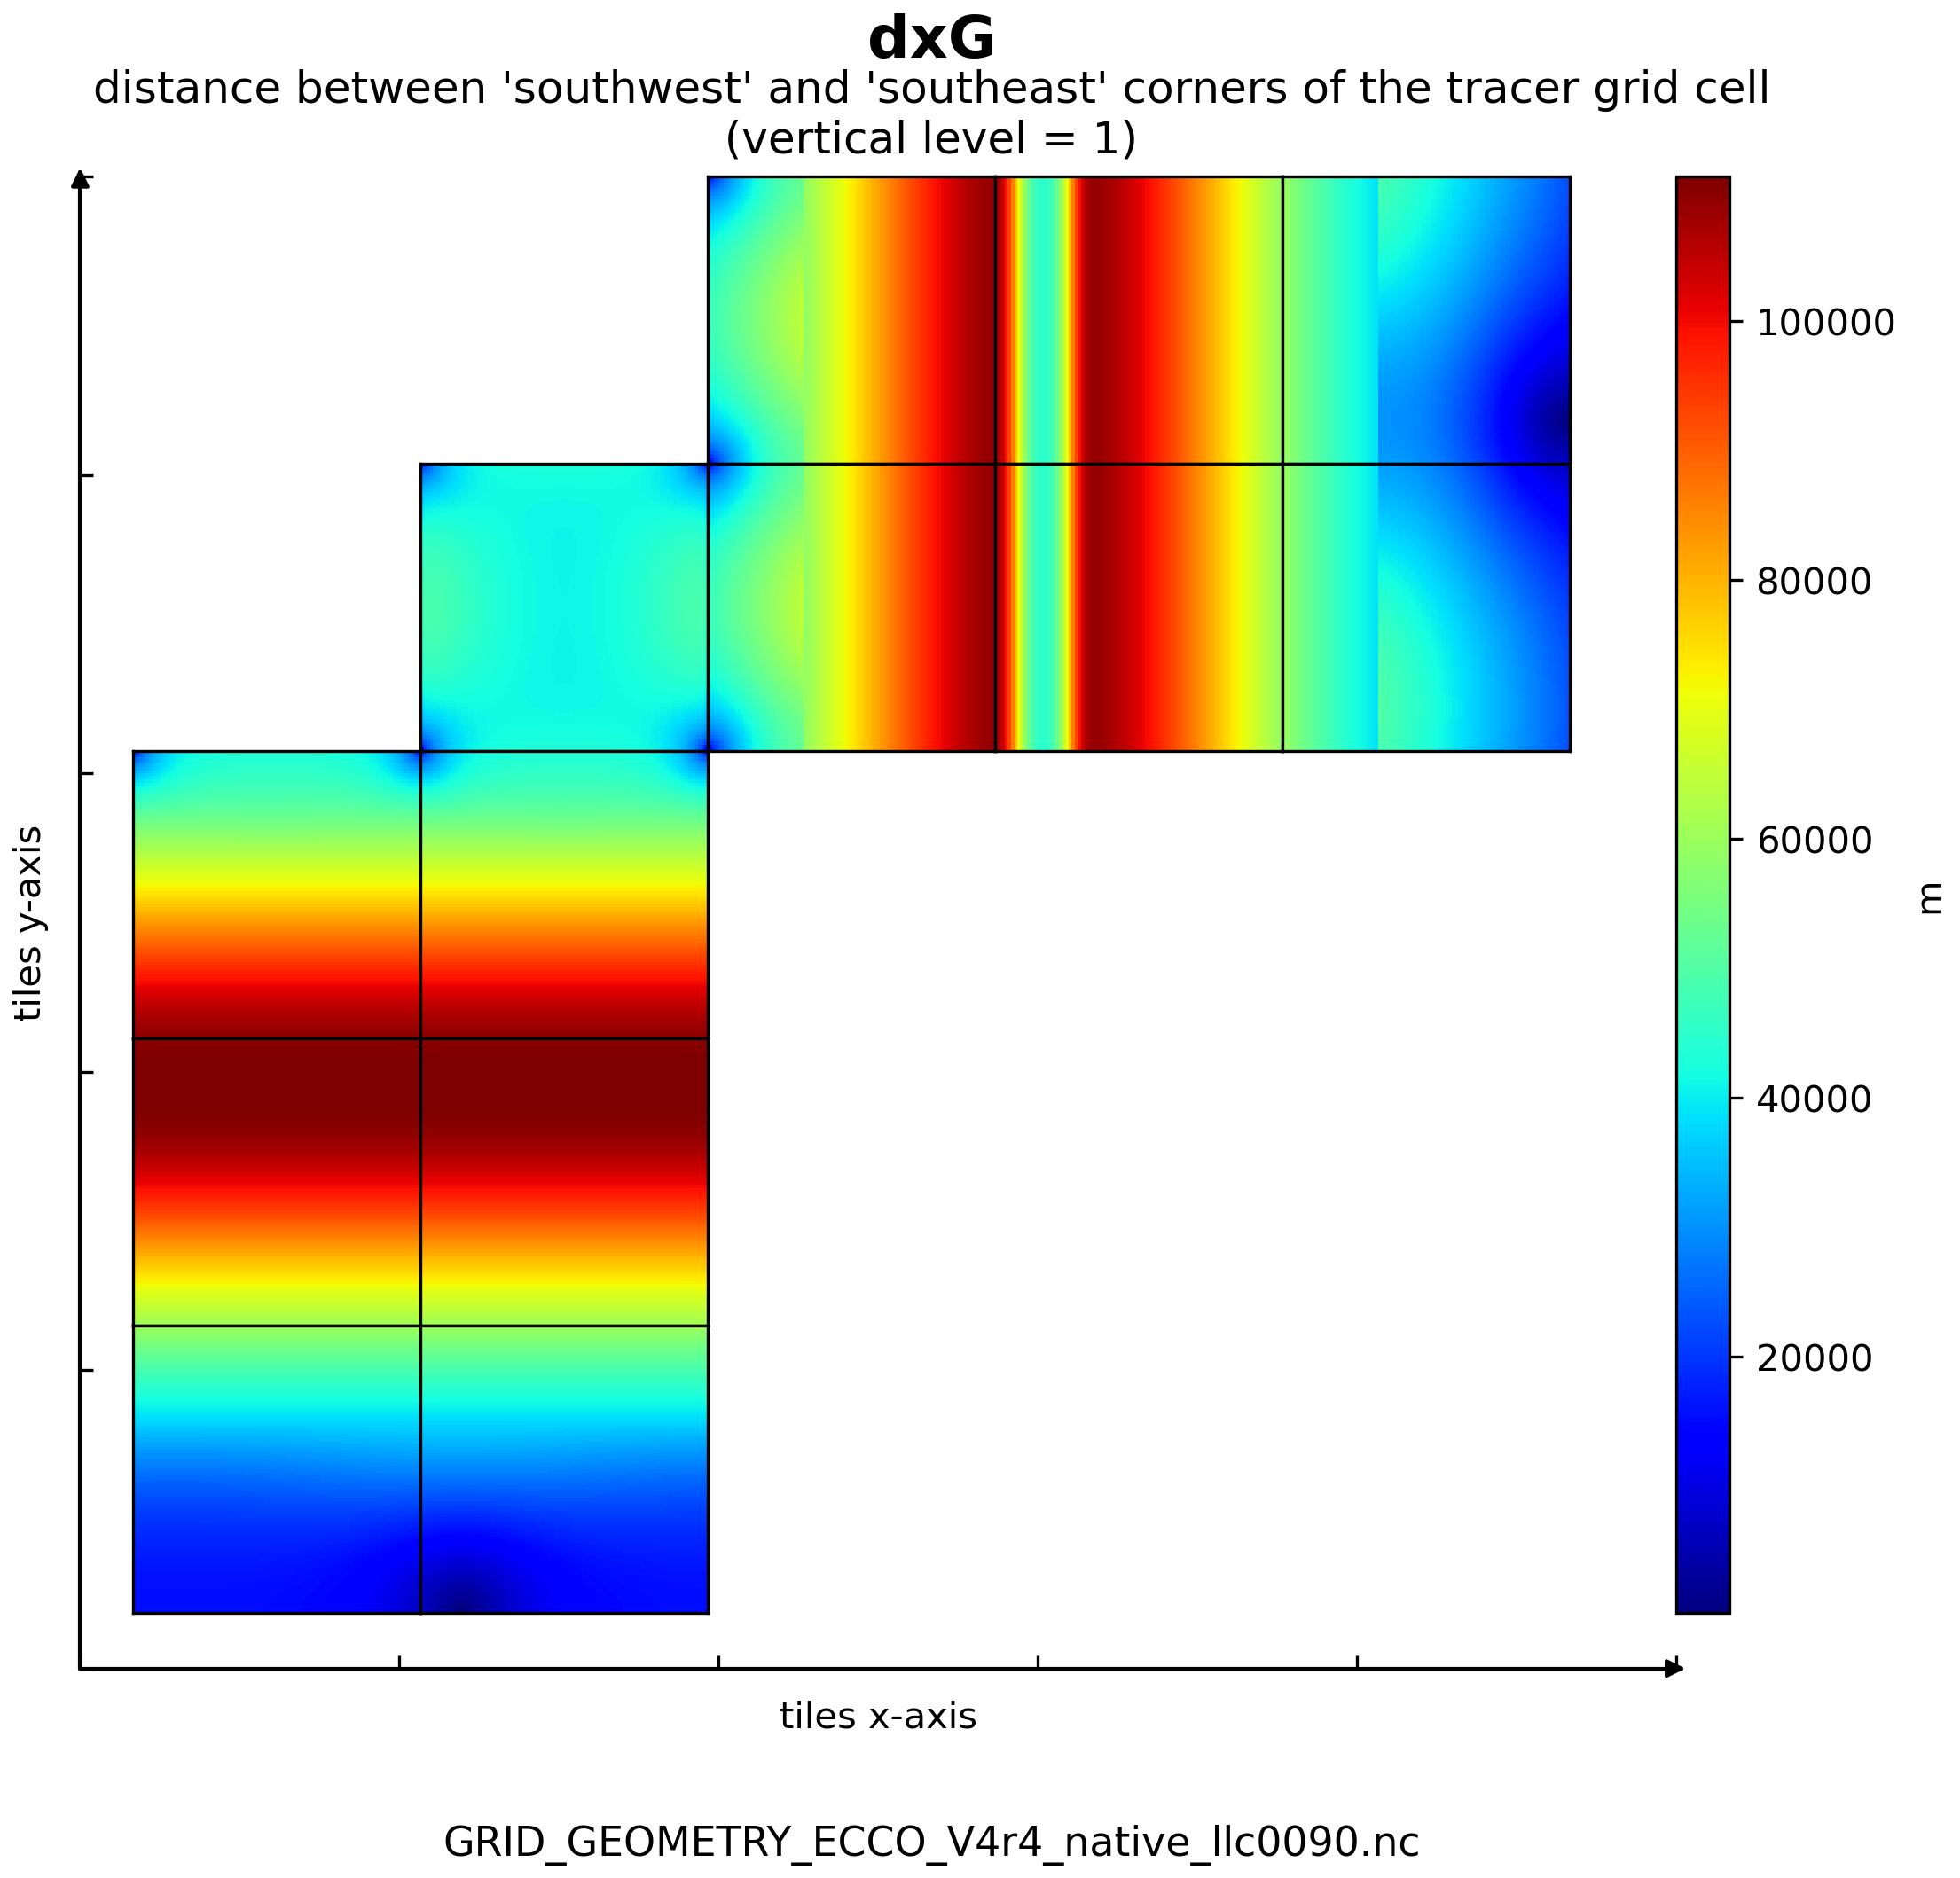
\includegraphics[scale=0.55]{../images/plots/v4r4/native_plots_coords/Geometry_Parameters_for_the_Lat-Lon-Cap_90_(llc90)_Native_Model_Grid_(Version_4_Release_4)/dxG.png}
\caption{Dataset: GRID\_GEOMETRY\_ECCO, Variable: dxG}
\label{tab:table-GRID_GEOMETRY_ECCO_dxG-Plot}
\end{figure}
\newpage
\pagebreak
\subsubsection{Native coordinates Variable: dyG}
\begin{longtable}{|m{0.06\textwidth}|m{0.3\textwidth}|m{0.45\textwidth}|m{0.12\textwidth}|}
\caption{Attributes description of the variable 'dyG' from GRID\_GEOMETRY\_ECCO's  dataset.}
\label{tab:table-GRID_GEOMETRY_ECCO_dyG} \\ 
\hline \endhead \hline \endfoot
\rowcolor{lightgray} \textbf{Storage Type} & \textbf{Variable Name} & \textbf{Description} & \textbf{Unit} \\ \hline
float32 & dyG & Distance between 'southwest' and 'northwest' corners of the tracer grid cell & m \\ \hline
\multicolumn{4}{|c|}{\cellcolor{lightgray}{\textbf{Description of the variable in Common Data language (CDL)}}} \\ \hline
\multicolumn{4}{|c|}{\fontfamily{lmtt}\selectfont{\makecell{\parbox{.95\textwidth}{\vspace*{0.25cm} \footnotesize{float32 dyG(tile, j, i\_g)\\
\hspace*{0.5cm}dyG: \_FillValue = 9.96921e+36\\
\hspace*{0.5cm}dyG: coordinate = YC XG\\
\hspace*{0.5cm}dyG: coverage\_content\_type = modelResult\\
\hspace*{0.5cm}dyG: long\_name = distance between southwest and northwest corners of the tracer grid cell\\
\hspace*{0.5cm}dyG: units = m\\
}}}}} \\ \hline
\rowcolor{lightgray} \multicolumn{4}{|c|}{\textbf{Comments}} \\ \hline
\multicolumn{4}{|p{1\textwidth}|}{\footnotesize{{Alternatively, the length of 'west' side of tracer grid cell. note: 'west, 'southwest', and 'northwest' do not correspond to geographic orientation but are used for convenience to describe the computational grid. see mitgcm documentation for details.}}} \\ \hline
\end{longtable}

\begin{figure}[H]
\centering
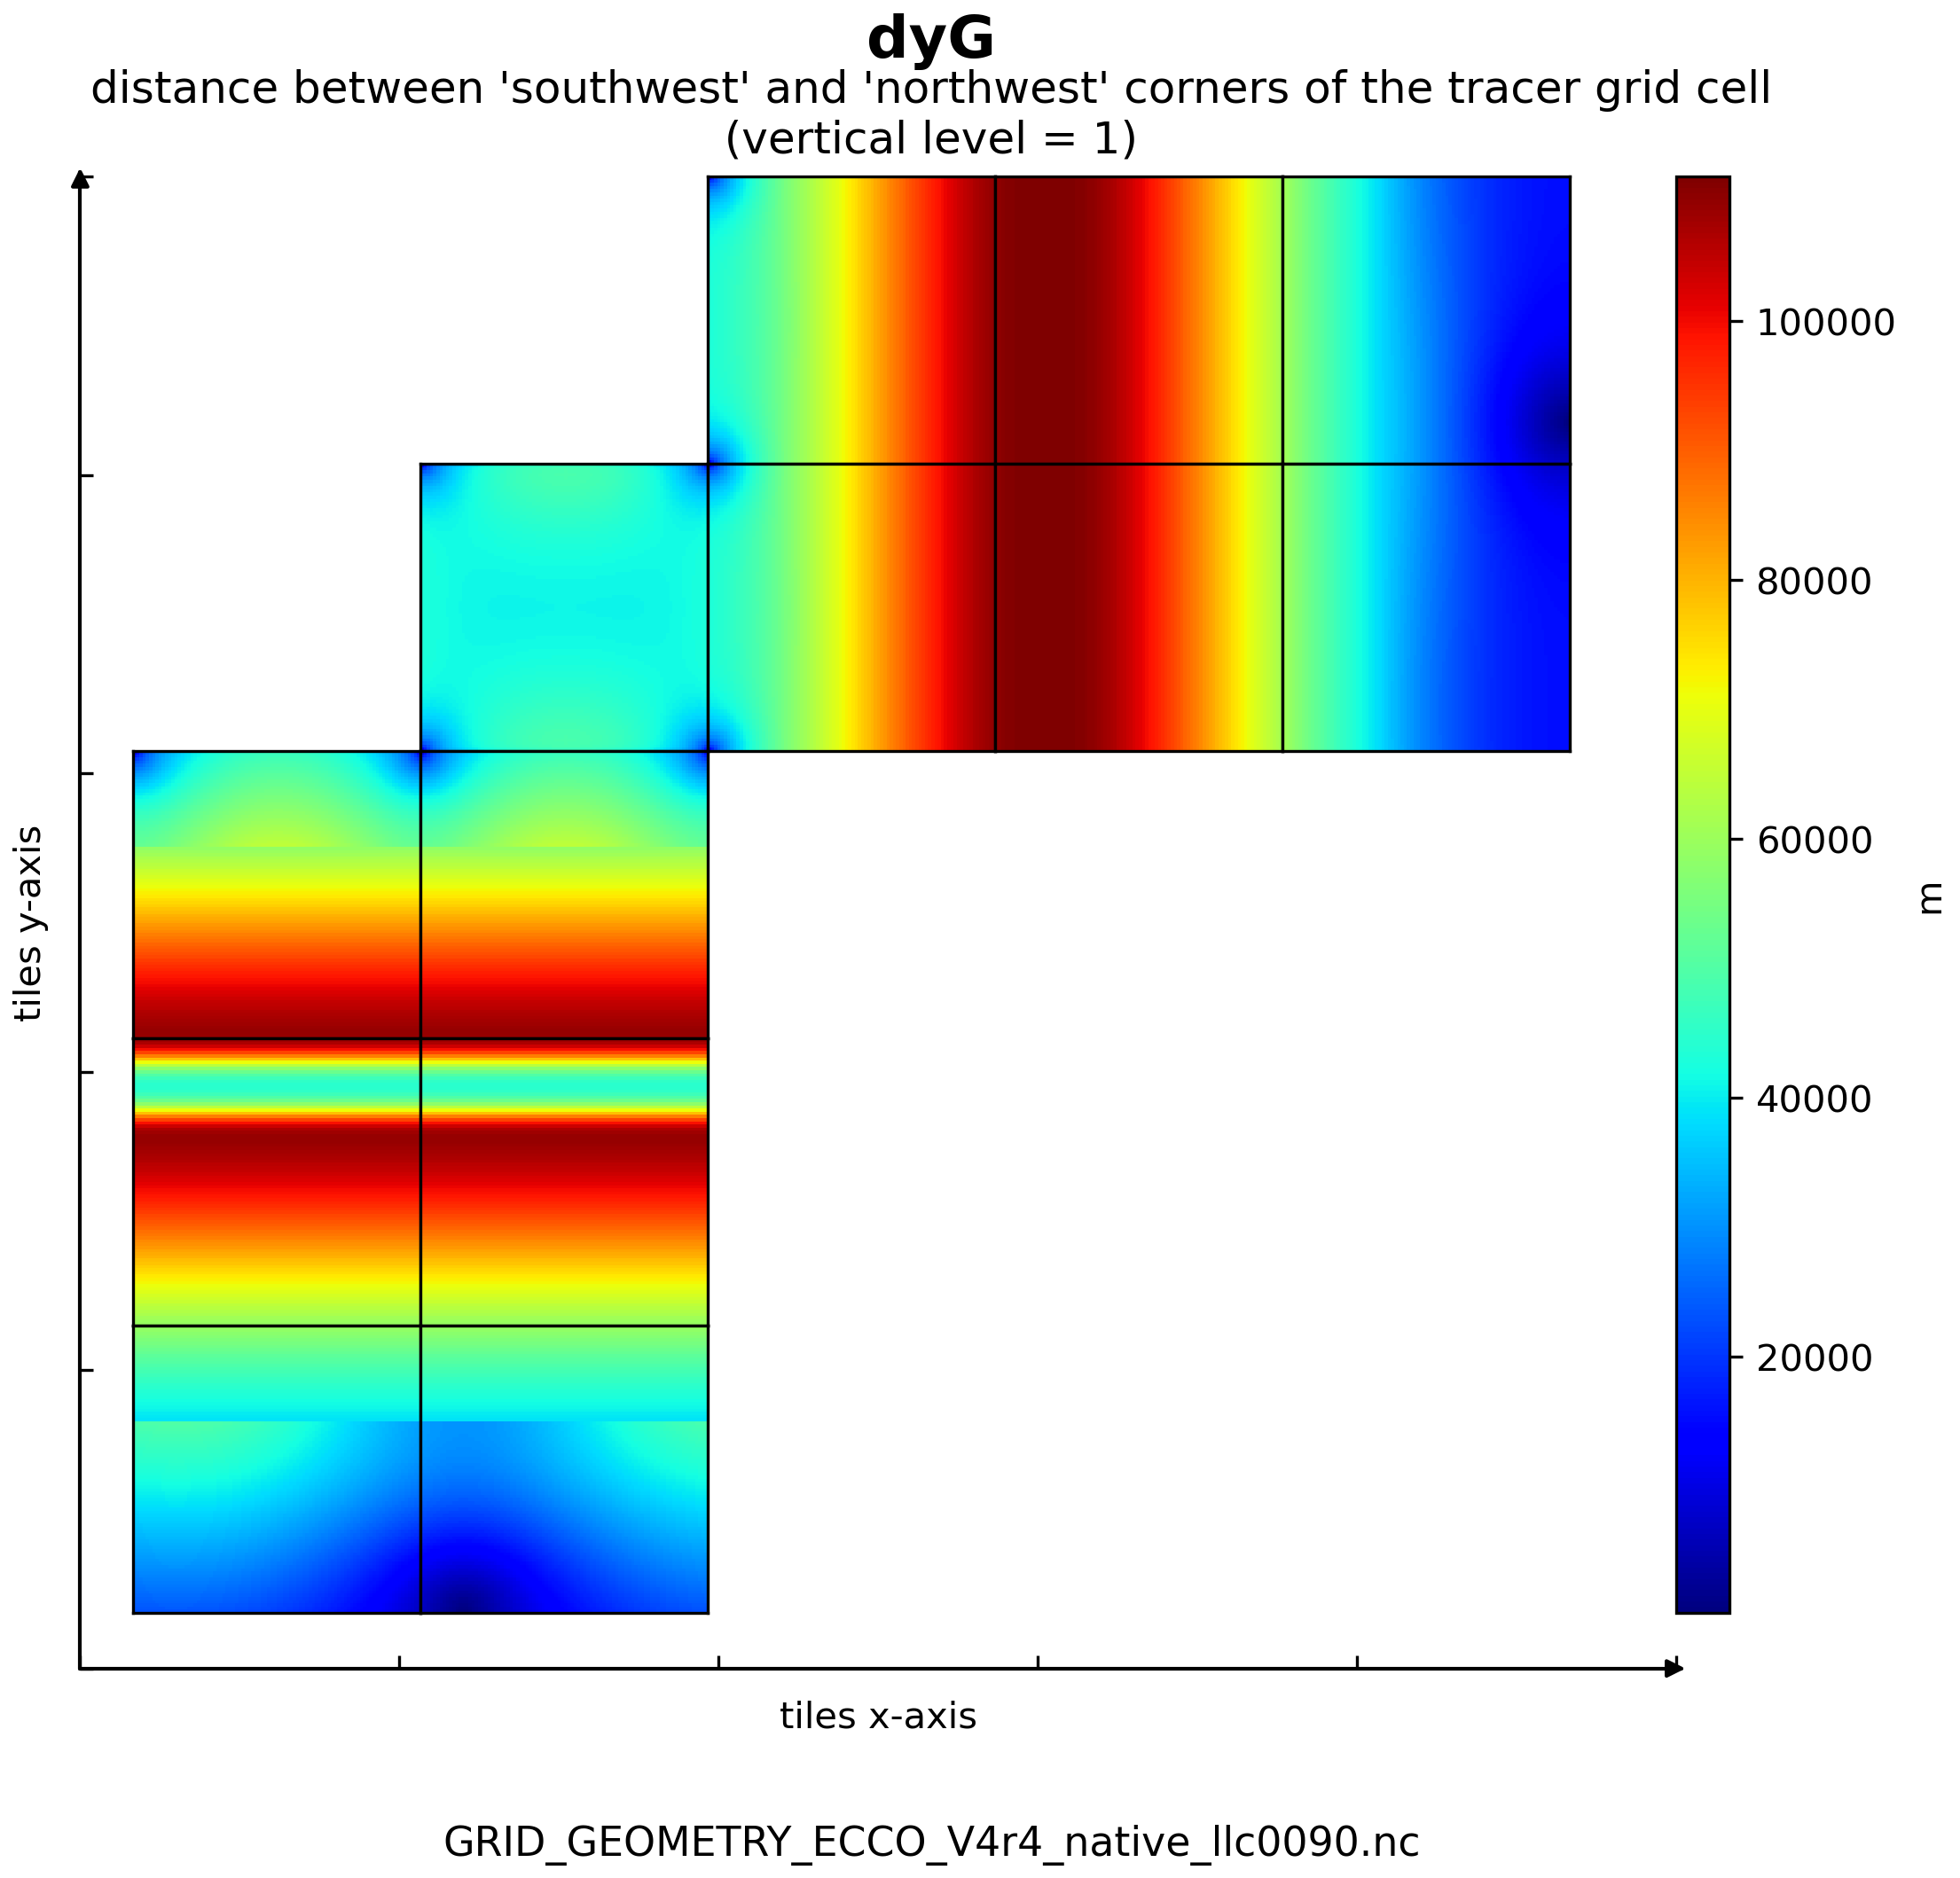
\includegraphics[scale=0.55]{../images/plots/v4r4/native_plots_coords/Geometry_Parameters_for_the_Lat-Lon-Cap_90_(llc90)_Native_Model_Grid_(Version_4_Release_4)/dyG.png}
\caption{Dataset: GRID\_GEOMETRY\_ECCO, Variable: dyG}
\label{tab:table-GRID_GEOMETRY_ECCO_dyG-Plot}
\end{figure}
\newpage
\pagebreak
\subsubsection{Native coordinates Variable: Depth}
\begin{longtable}{|m{0.06\textwidth}|m{0.3\textwidth}|m{0.45\textwidth}|m{0.12\textwidth}|}
\caption{Attributes description of the variable 'Depth' from GRID\_GEOMETRY\_ECCO's  dataset.}
\label{tab:table-GRID_GEOMETRY_ECCO_Depth} \\ 
\hline \endhead \hline \endfoot
\rowcolor{lightgray} \textbf{Storage Type} & \textbf{Variable Name} & \textbf{Description} & \textbf{Unit} \\ \hline
float32 & Depth & Model seafloor depth below ocean surface at rest & m \\ \hline
\multicolumn{4}{|c|}{\cellcolor{lightgray}{\textbf{Description of the variable in Common Data language (CDL)}}} \\ \hline
\multicolumn{4}{|c|}{\fontfamily{lmtt}\selectfont{\makecell{\parbox{.95\textwidth}{\vspace*{0.25cm} \footnotesize{float32 Depth(tile, j, i)\\
\hspace*{0.5cm}Depth: \_FillValue = 9.96921e+36\\
\hspace*{0.5cm}Depth: coordinate = XC YC\\
\hspace*{0.5cm}Depth: coordinates = YC XC\\
\hspace*{0.5cm}Depth: coverage\_content\_type = modelResult\\
\hspace*{0.5cm}Depth: long\_name = model seafloor depth below ocean surface at rest\\
\hspace*{0.5cm}Depth: standard\_name = sea floor depth below geoid\\
\hspace*{0.5cm}Depth: units = m\\
}}}}} \\ \hline
\rowcolor{lightgray} \multicolumn{4}{|c|}{\textbf{Comments}} \\ \hline
\multicolumn{4}{|p{1\textwidth}|}{\footnotesize{{Model sea surface height (ssh) of 0m corresponds to an ocean surface at rest relative to the geoid. depth corresponds to seafloor depth below geoid. note: the mitgcm used by ecco v4r4 implements 'partial cells' so the actual model seafloor depth may differ from the seafloor depth provided by the input bathymetry file.}}} \\ \hline
\end{longtable}

\begin{figure}[H]
\centering
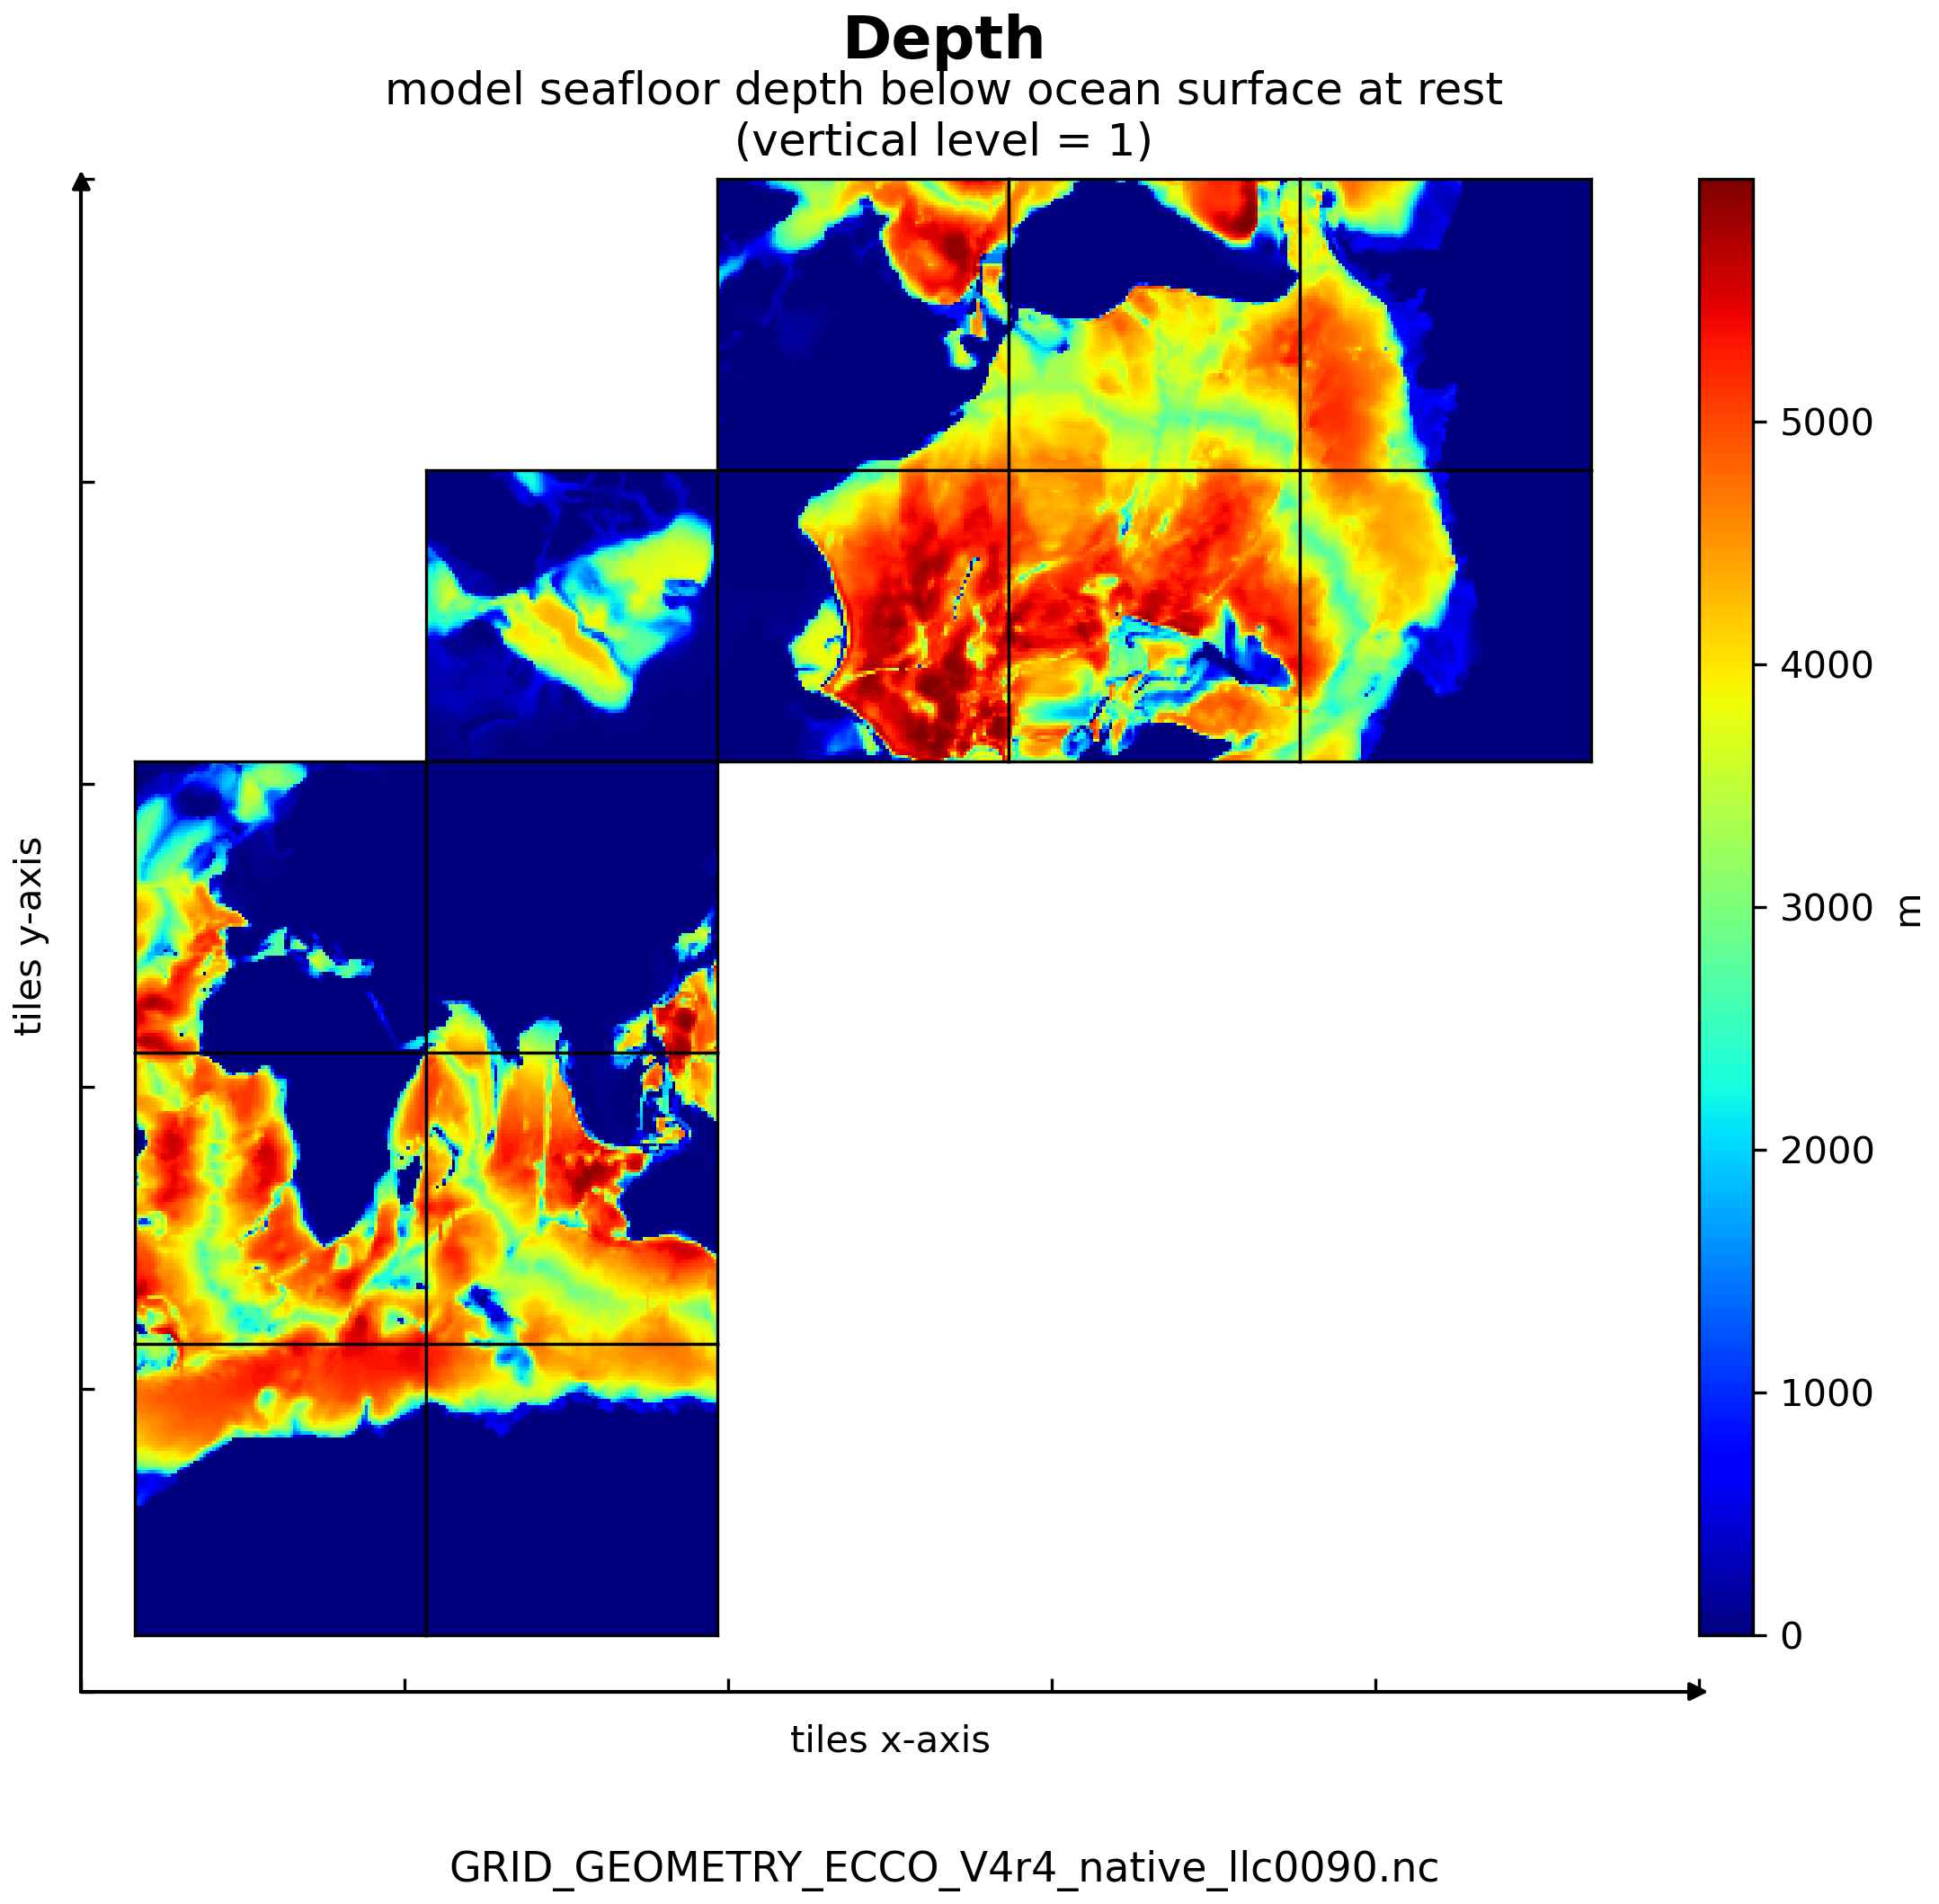
\includegraphics[scale=0.55]{../images/plots/v4r4/native_plots_coords/Geometry_Parameters_for_the_Lat-Lon-Cap_90_(llc90)_Native_Model_Grid_(Version_4_Release_4)/Depth.png}
\caption{Dataset: GRID\_GEOMETRY\_ECCO, Variable: Depth}
\label{tab:table-GRID_GEOMETRY_ECCO_Depth-Plot}
\end{figure}
\newpage
\pagebreak
\subsubsection{Native coordinates Variable: rAz}
\begin{longtable}{|m{0.06\textwidth}|m{0.3\textwidth}|m{0.45\textwidth}|m{0.12\textwidth}|}
\caption{Attributes description of the variable 'rAz' from GRID\_GEOMETRY\_ECCO's  dataset.}
\label{tab:table-GRID_GEOMETRY_ECCO_rAz} \\ 
\hline \endhead \hline \endfoot
\rowcolor{lightgray} \textbf{Storage Type} & \textbf{Variable Name} & \textbf{Description} & \textbf{Unit} \\ \hline
float32 & rAz & Area of vorticity 'g' grid cell & m2 \\ \hline
\multicolumn{4}{|c|}{\cellcolor{lightgray}{\textbf{Description of the variable in Common Data language (CDL)}}} \\ \hline
\multicolumn{4}{|c|}{\fontfamily{lmtt}\selectfont{\makecell{\parbox{.95\textwidth}{\vspace*{0.25cm} \footnotesize{float32 rAz(tile, j\_g, i\_g)\\
\hspace*{0.5cm}rAz: \_FillValue = 9.96921e+36\\
\hspace*{0.5cm}rAz: coordinate = YG XG\\
\hspace*{0.5cm}rAz: coordinates = YG XG\\
\hspace*{0.5cm}rAz: coverage\_content\_type = modelResult\\
\hspace*{0.5cm}rAz: long\_name = area of vorticity g grid cell\\
\hspace*{0.5cm}rAz: standard\_name = cell area\\
\hspace*{0.5cm}rAz: units = m2\\
}}}}} \\ \hline
\rowcolor{lightgray} \multicolumn{4}{|c|}{\textbf{Comments}} \\ \hline
\multicolumn{4}{|p{1\textwidth}|}{\footnotesize{{Vorticity cells are staggered in space relative to tracer cells, nominally situated on tracer cell corners. vorticity cell (i,j) is located at the 'southwest' corner of tracer grid cell (i, j). note: 'southwest' does not correspond to geographic orientation but is used for convenience to describe the computational grid. see mitgcm documentation for details.}}} \\ \hline
\end{longtable}

\begin{figure}[H]
\centering
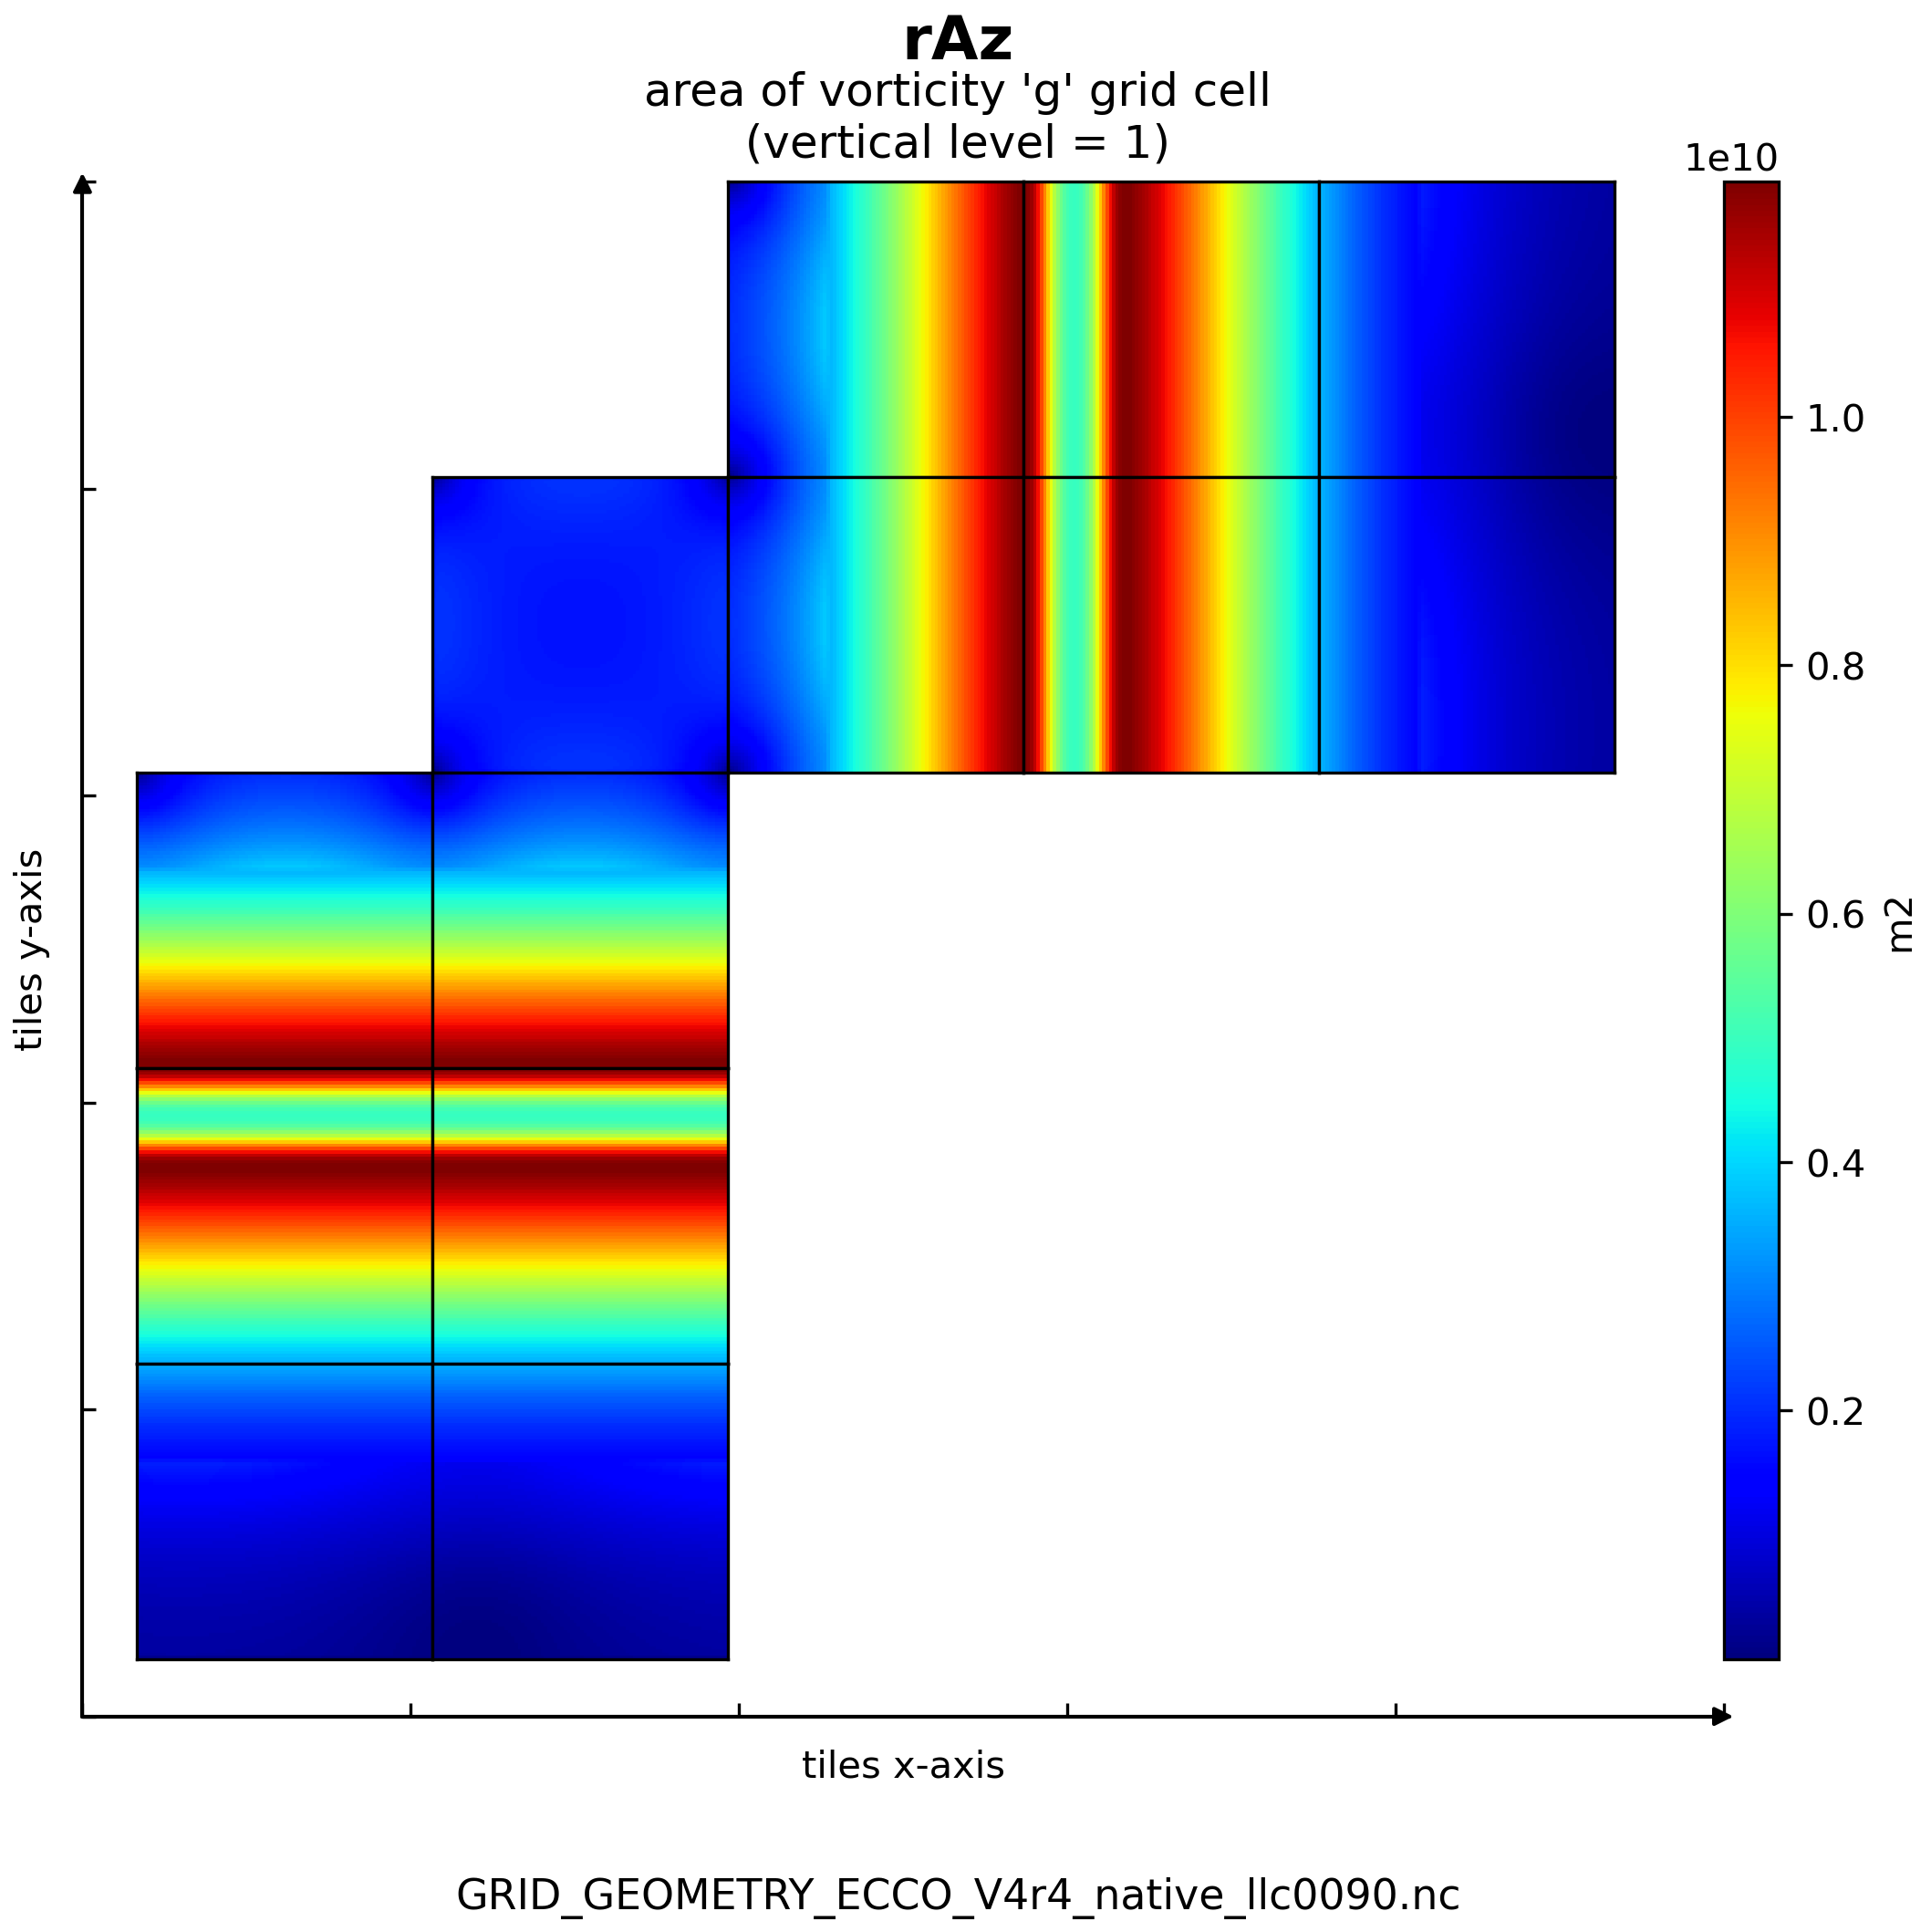
\includegraphics[scale=0.55]{../images/plots/v4r4/native_plots_coords/Geometry_Parameters_for_the_Lat-Lon-Cap_90_(llc90)_Native_Model_Grid_(Version_4_Release_4)/rAz.png}
\caption{Dataset: GRID\_GEOMETRY\_ECCO, Variable: rAz}
\label{tab:table-GRID_GEOMETRY_ECCO_rAz-Plot}
\end{figure}
\newpage
\pagebreak
\subsubsection{Native coordinates Variable: dxC}
\begin{longtable}{|m{0.06\textwidth}|m{0.3\textwidth}|m{0.45\textwidth}|m{0.12\textwidth}|}
\caption{Attributes description of the variable 'dxC' from GRID\_GEOMETRY\_ECCO's  dataset.}
\label{tab:table-GRID_GEOMETRY_ECCO_dxC} \\ 
\hline \endhead \hline \endfoot
\rowcolor{lightgray} \textbf{Storage Type} & \textbf{Variable Name} & \textbf{Description} & \textbf{Unit} \\ \hline
float32 & dxC & Distance between centers of adjacent tracer grid cells in the 'x' direction & m \\ \hline
\multicolumn{4}{|c|}{\cellcolor{lightgray}{\textbf{Description of the variable in Common Data language (CDL)}}} \\ \hline
\multicolumn{4}{|c|}{\fontfamily{lmtt}\selectfont{\makecell{\parbox{.95\textwidth}{\vspace*{0.25cm} \footnotesize{float32 dxC(tile, j, i\_g)\\
\hspace*{0.5cm}dxC: \_FillValue = 9.96921e+36\\
\hspace*{0.5cm}dxC: coordinate = YC XG\\
\hspace*{0.5cm}dxC: coverage\_content\_type = modelResult\\
\hspace*{0.5cm}dxC: long\_name = distance between centers of adjacent tracer grid cells in the x direction\\
\hspace*{0.5cm}dxC: units = m\\
}}}}} \\ \hline
\rowcolor{lightgray} \multicolumn{4}{|c|}{\textbf{Comments}} \\ \hline
\multicolumn{4}{|p{1\textwidth}|}{\footnotesize{{Alternatively, the length of 'north' side of vorticity grid cells. note: 'north' does not correspond to geographic orientation but is used for convenience to describe the computational grid. see mitgcm documentation for details.}}} \\ \hline
\end{longtable}

\begin{figure}[H]
\centering
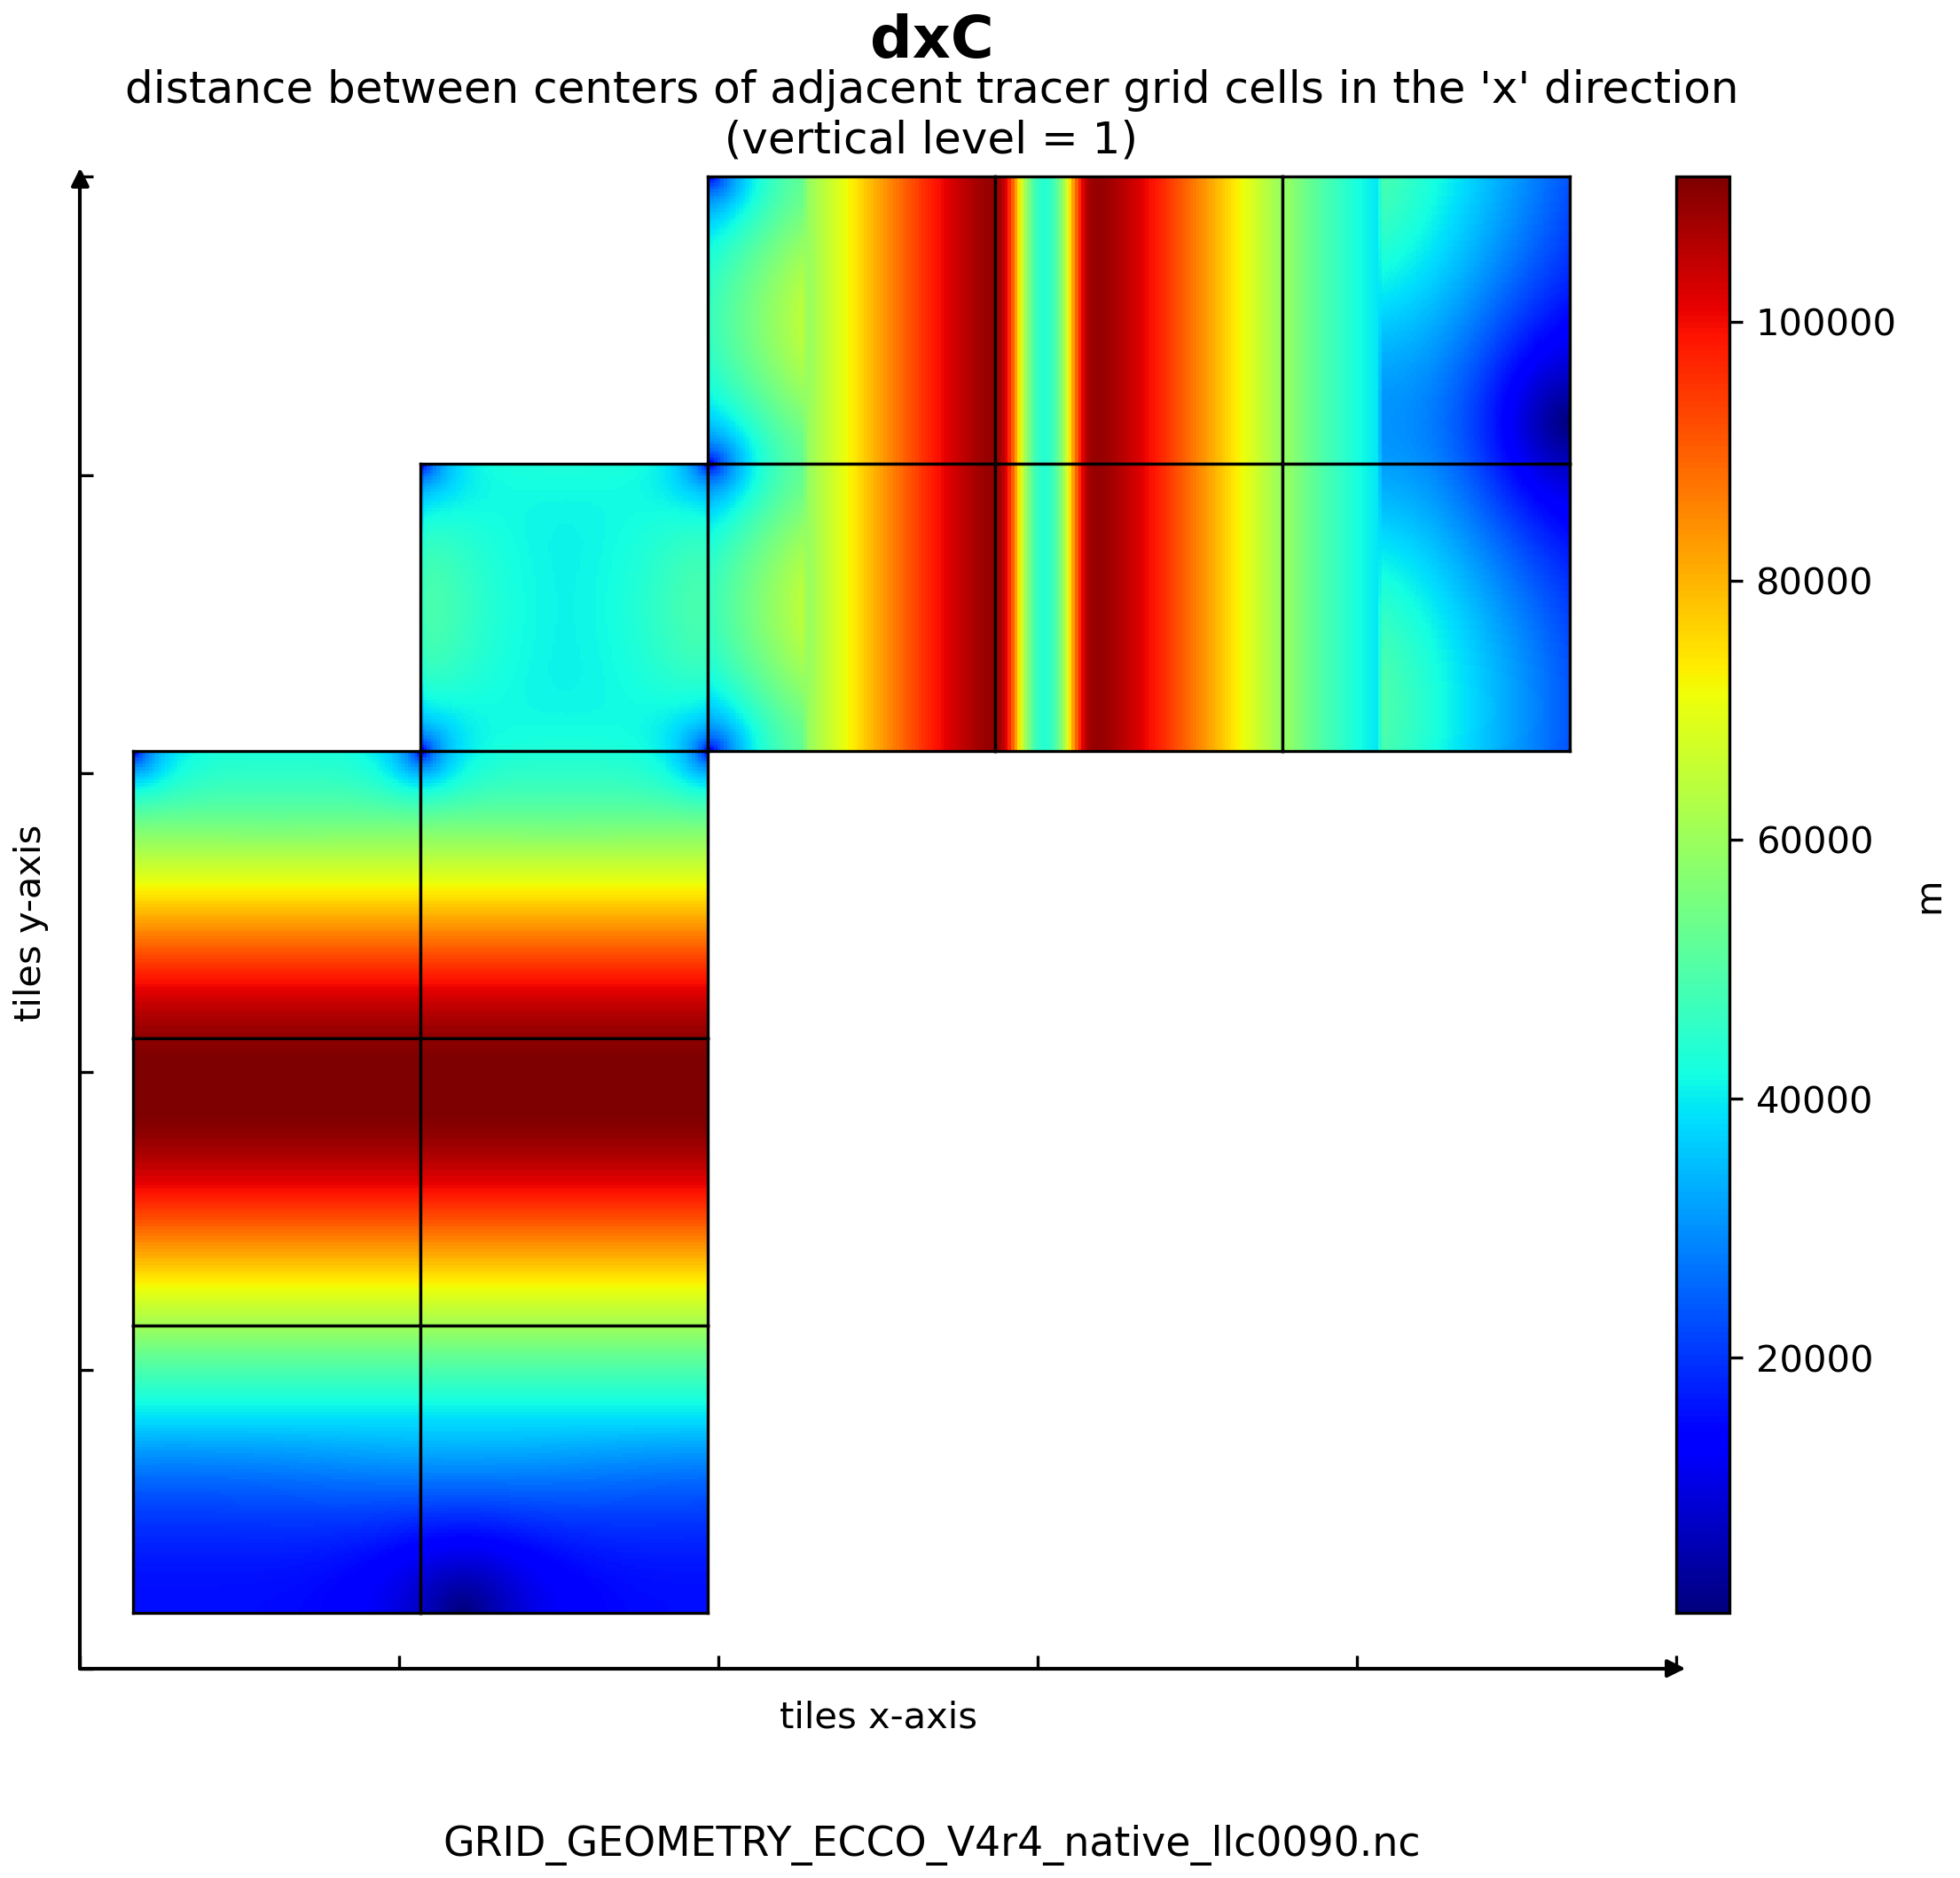
\includegraphics[scale=0.55]{../images/plots/v4r4/native_plots_coords/Geometry_Parameters_for_the_Lat-Lon-Cap_90_(llc90)_Native_Model_Grid_(Version_4_Release_4)/dxC.png}
\caption{Dataset: GRID\_GEOMETRY\_ECCO, Variable: dxC}
\label{tab:table-GRID_GEOMETRY_ECCO_dxC-Plot}
\end{figure}
\newpage
\pagebreak
\subsubsection{Native coordinates Variable: dyC}
\begin{longtable}{|m{0.06\textwidth}|m{0.3\textwidth}|m{0.45\textwidth}|m{0.12\textwidth}|}
\caption{Attributes description of the variable 'dyC' from GRID\_GEOMETRY\_ECCO's  dataset.}
\label{tab:table-GRID_GEOMETRY_ECCO_dyC} \\ 
\hline \endhead \hline \endfoot
\rowcolor{lightgray} \textbf{Storage Type} & \textbf{Variable Name} & \textbf{Description} & \textbf{Unit} \\ \hline
float32 & dyC & Distance between centers of adjacent tracer grid cells in the 'y' direction & m \\ \hline
\multicolumn{4}{|c|}{\cellcolor{lightgray}{\textbf{Description of the variable in Common Data language (CDL)}}} \\ \hline
\multicolumn{4}{|c|}{\fontfamily{lmtt}\selectfont{\makecell{\parbox{.95\textwidth}{\vspace*{0.25cm} \footnotesize{float32 dyC(tile, j\_g, i)\\
\hspace*{0.5cm}dyC: \_FillValue = 9.96921e+36\\
\hspace*{0.5cm}dyC: coordinate = YG XC\\
\hspace*{0.5cm}dyC: coverage\_content\_type = modelResult\\
\hspace*{0.5cm}dyC: long\_name = distance between centers of adjacent tracer grid cells in the y direction\\
\hspace*{0.5cm}dyC: units = m\\
}}}}} \\ \hline
\rowcolor{lightgray} \multicolumn{4}{|c|}{\textbf{Comments}} \\ \hline
\multicolumn{4}{|p{1\textwidth}|}{\footnotesize{{Alternatively, the length of 'east' side of vorticity grid cells. note: 'east' does not correspond to geographic orientation but is used for convenience to describe the computational grid. see mitgcm documentation for details.}}} \\ \hline
\end{longtable}

\begin{figure}[H]
\centering
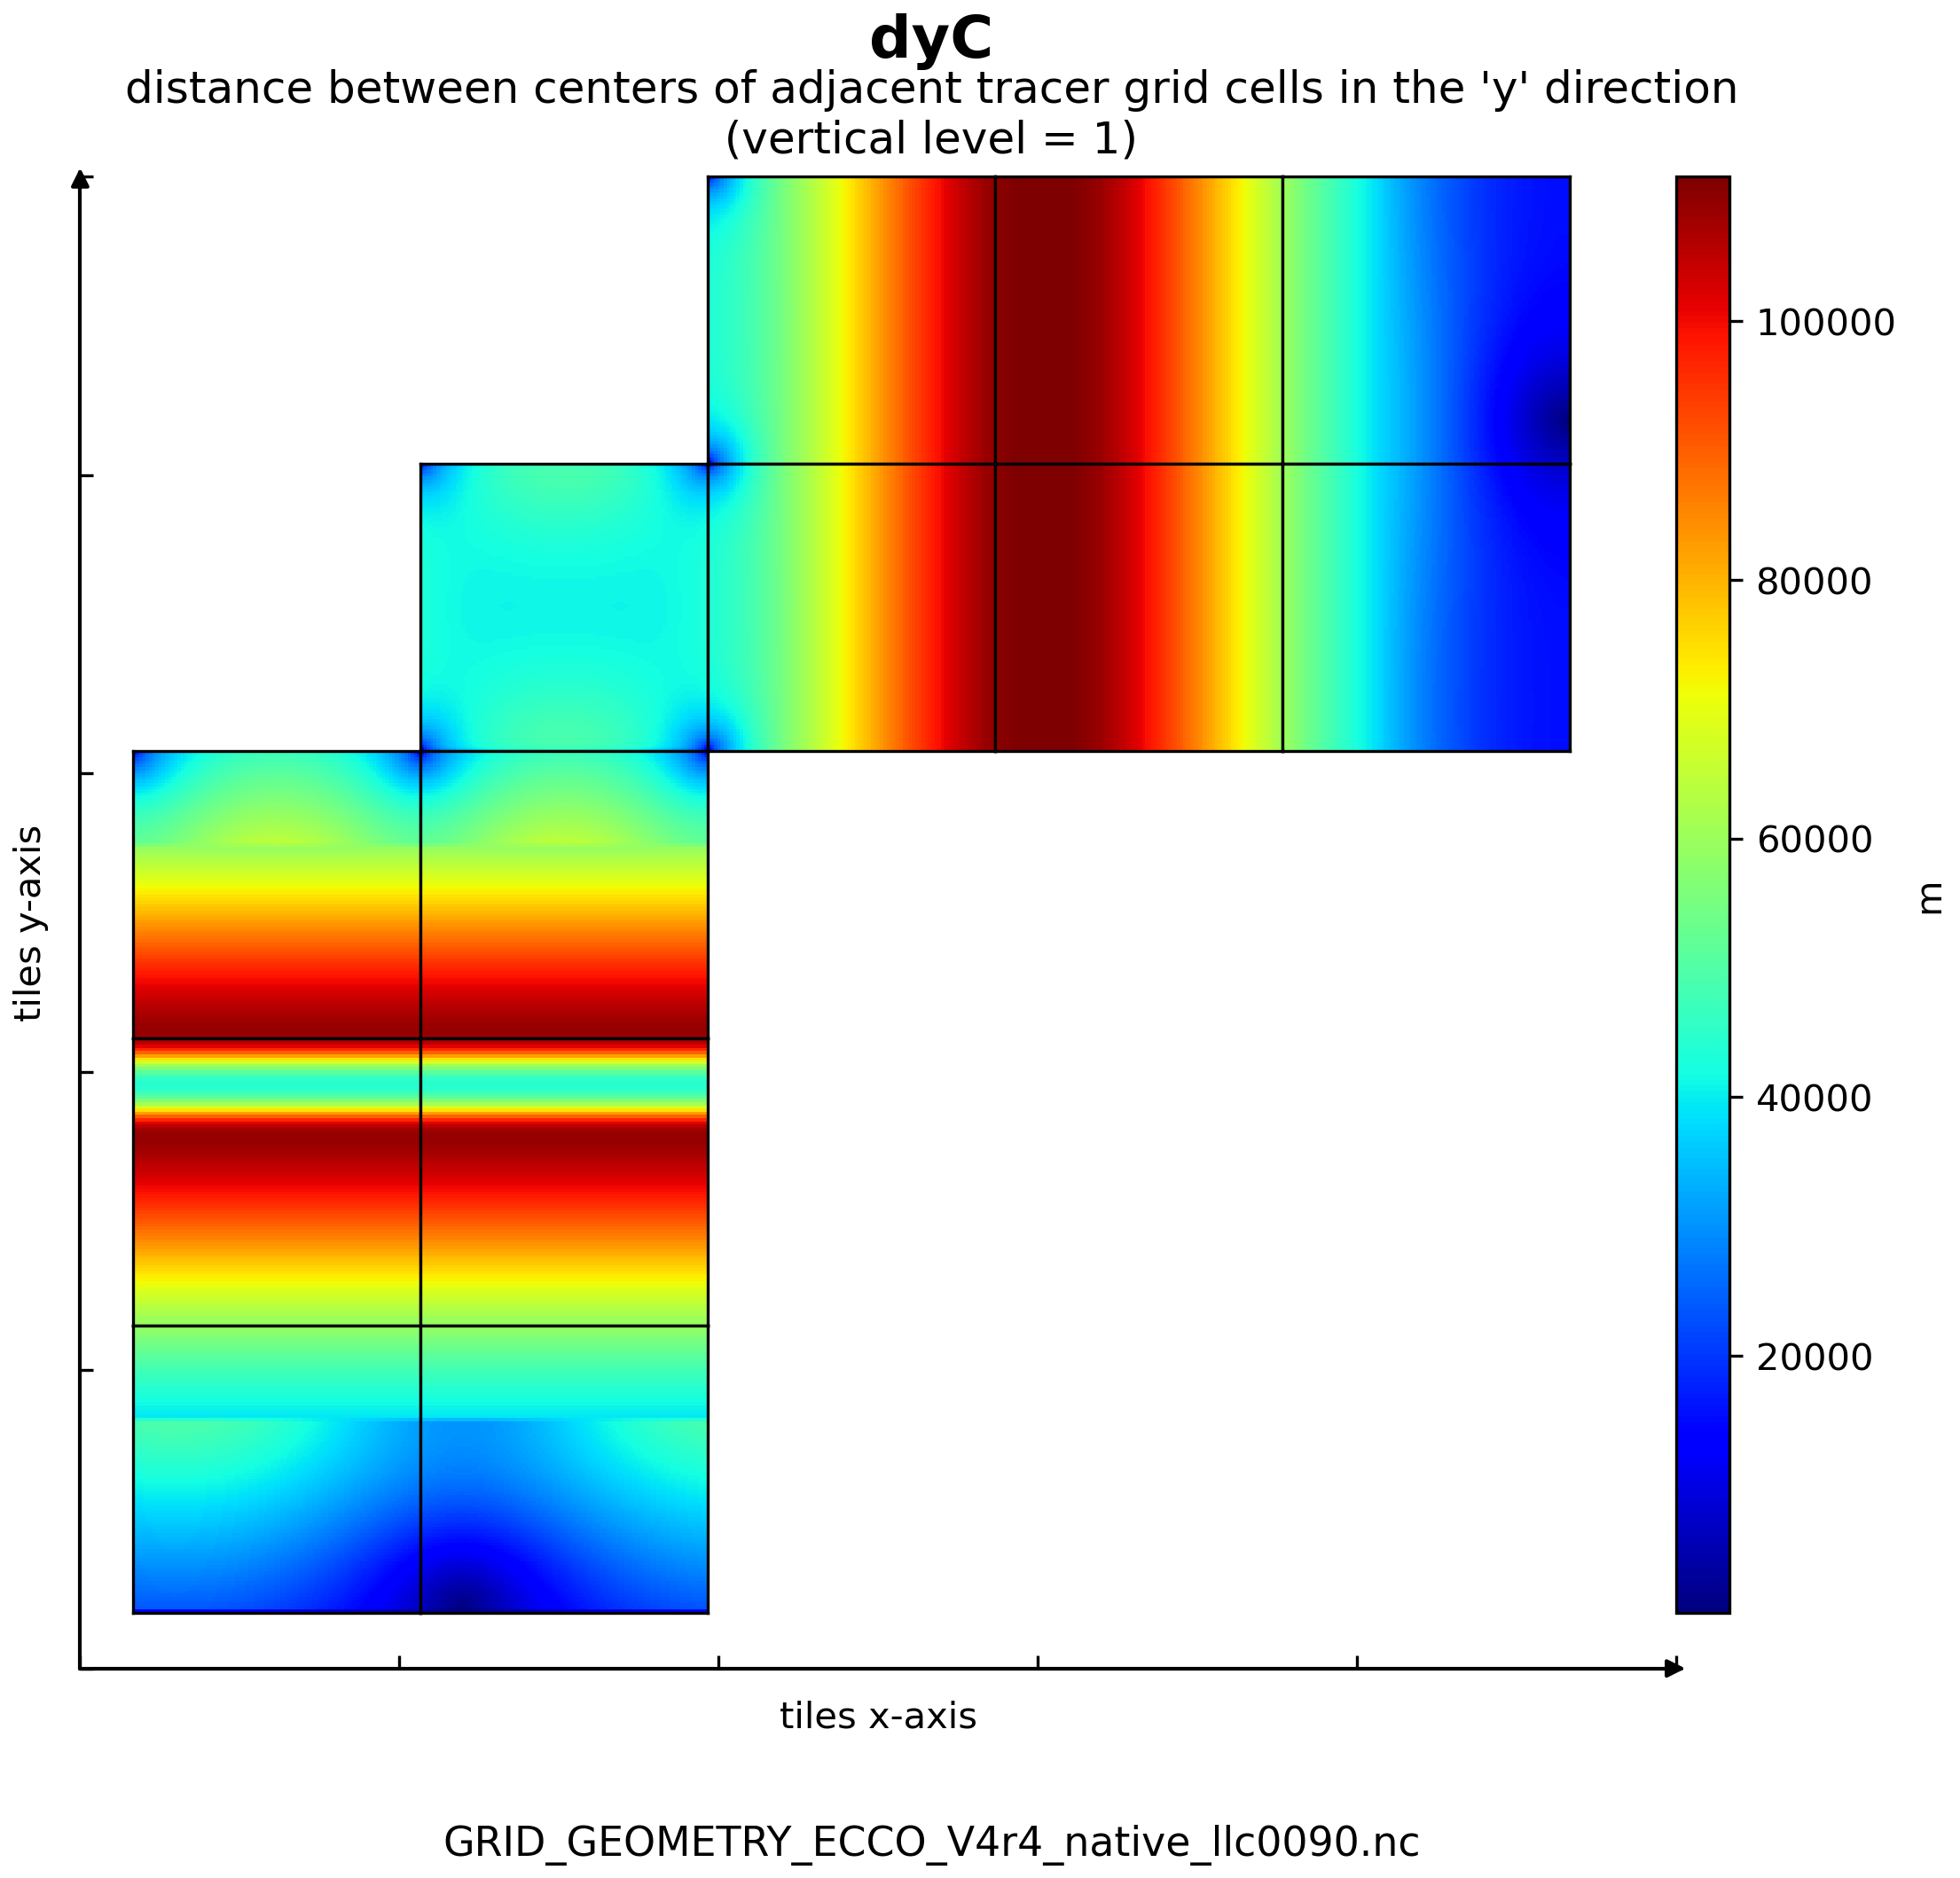
\includegraphics[scale=0.55]{../images/plots/v4r4/native_plots_coords/Geometry_Parameters_for_the_Lat-Lon-Cap_90_(llc90)_Native_Model_Grid_(Version_4_Release_4)/dyC.png}
\caption{Dataset: GRID\_GEOMETRY\_ECCO, Variable: dyC}
\label{tab:table-GRID_GEOMETRY_ECCO_dyC-Plot}
\end{figure}
\newpage
\pagebreak
\subsubsection{Native coordinates Variable: rAw}
\begin{longtable}{|m{0.06\textwidth}|m{0.3\textwidth}|m{0.45\textwidth}|m{0.12\textwidth}|}
\caption{Attributes description of the variable 'rAw' from GRID\_GEOMETRY\_ECCO's  dataset.}
\label{tab:table-GRID_GEOMETRY_ECCO_rAw} \\ 
\hline \endhead \hline \endfoot
\rowcolor{lightgray} \textbf{Storage Type} & \textbf{Variable Name} & \textbf{Description} & \textbf{Unit} \\ \hline
float32 & rAw & Area of 'v' grid cell & m2 \\ \hline
\multicolumn{4}{|c|}{\cellcolor{lightgray}{\textbf{Description of the variable in Common Data language (CDL)}}} \\ \hline
\multicolumn{4}{|c|}{\fontfamily{lmtt}\selectfont{\makecell{\parbox{.95\textwidth}{\vspace*{0.25cm} \footnotesize{float32 rAw(tile, j, i\_g)\\
\hspace*{0.5cm}rAw: \_FillValue = 9.96921e+36\\
\hspace*{0.5cm}rAw: coordinate = YG XC\\
\hspace*{0.5cm}rAw: coverage\_content\_type = modelResult\\
\hspace*{0.5cm}rAw: long\_name = area of v grid cell\\
\hspace*{0.5cm}rAw: standard\_name = cell area\\
\hspace*{0.5cm}rAw: units = m2\\
}}}}} \\ \hline
\rowcolor{lightgray} \multicolumn{4}{|c|}{\textbf{Comments}} \\ \hline
\multicolumn{4}{|p{1\textwidth}|}{\footnotesize{{Model 'v' grid cells are staggered in space between adjacent tracer grid cells in the 'x' direction. 'v' grid cell (i,j) is situated at the 'west' edge of tracer grid cell (i, j). note: 'west' does not correspond to geographic orientation but is used for convenience to describe the computational grid. see mitgcm documentation for details.}}} \\ \hline
\end{longtable}

\begin{figure}[H]
\centering
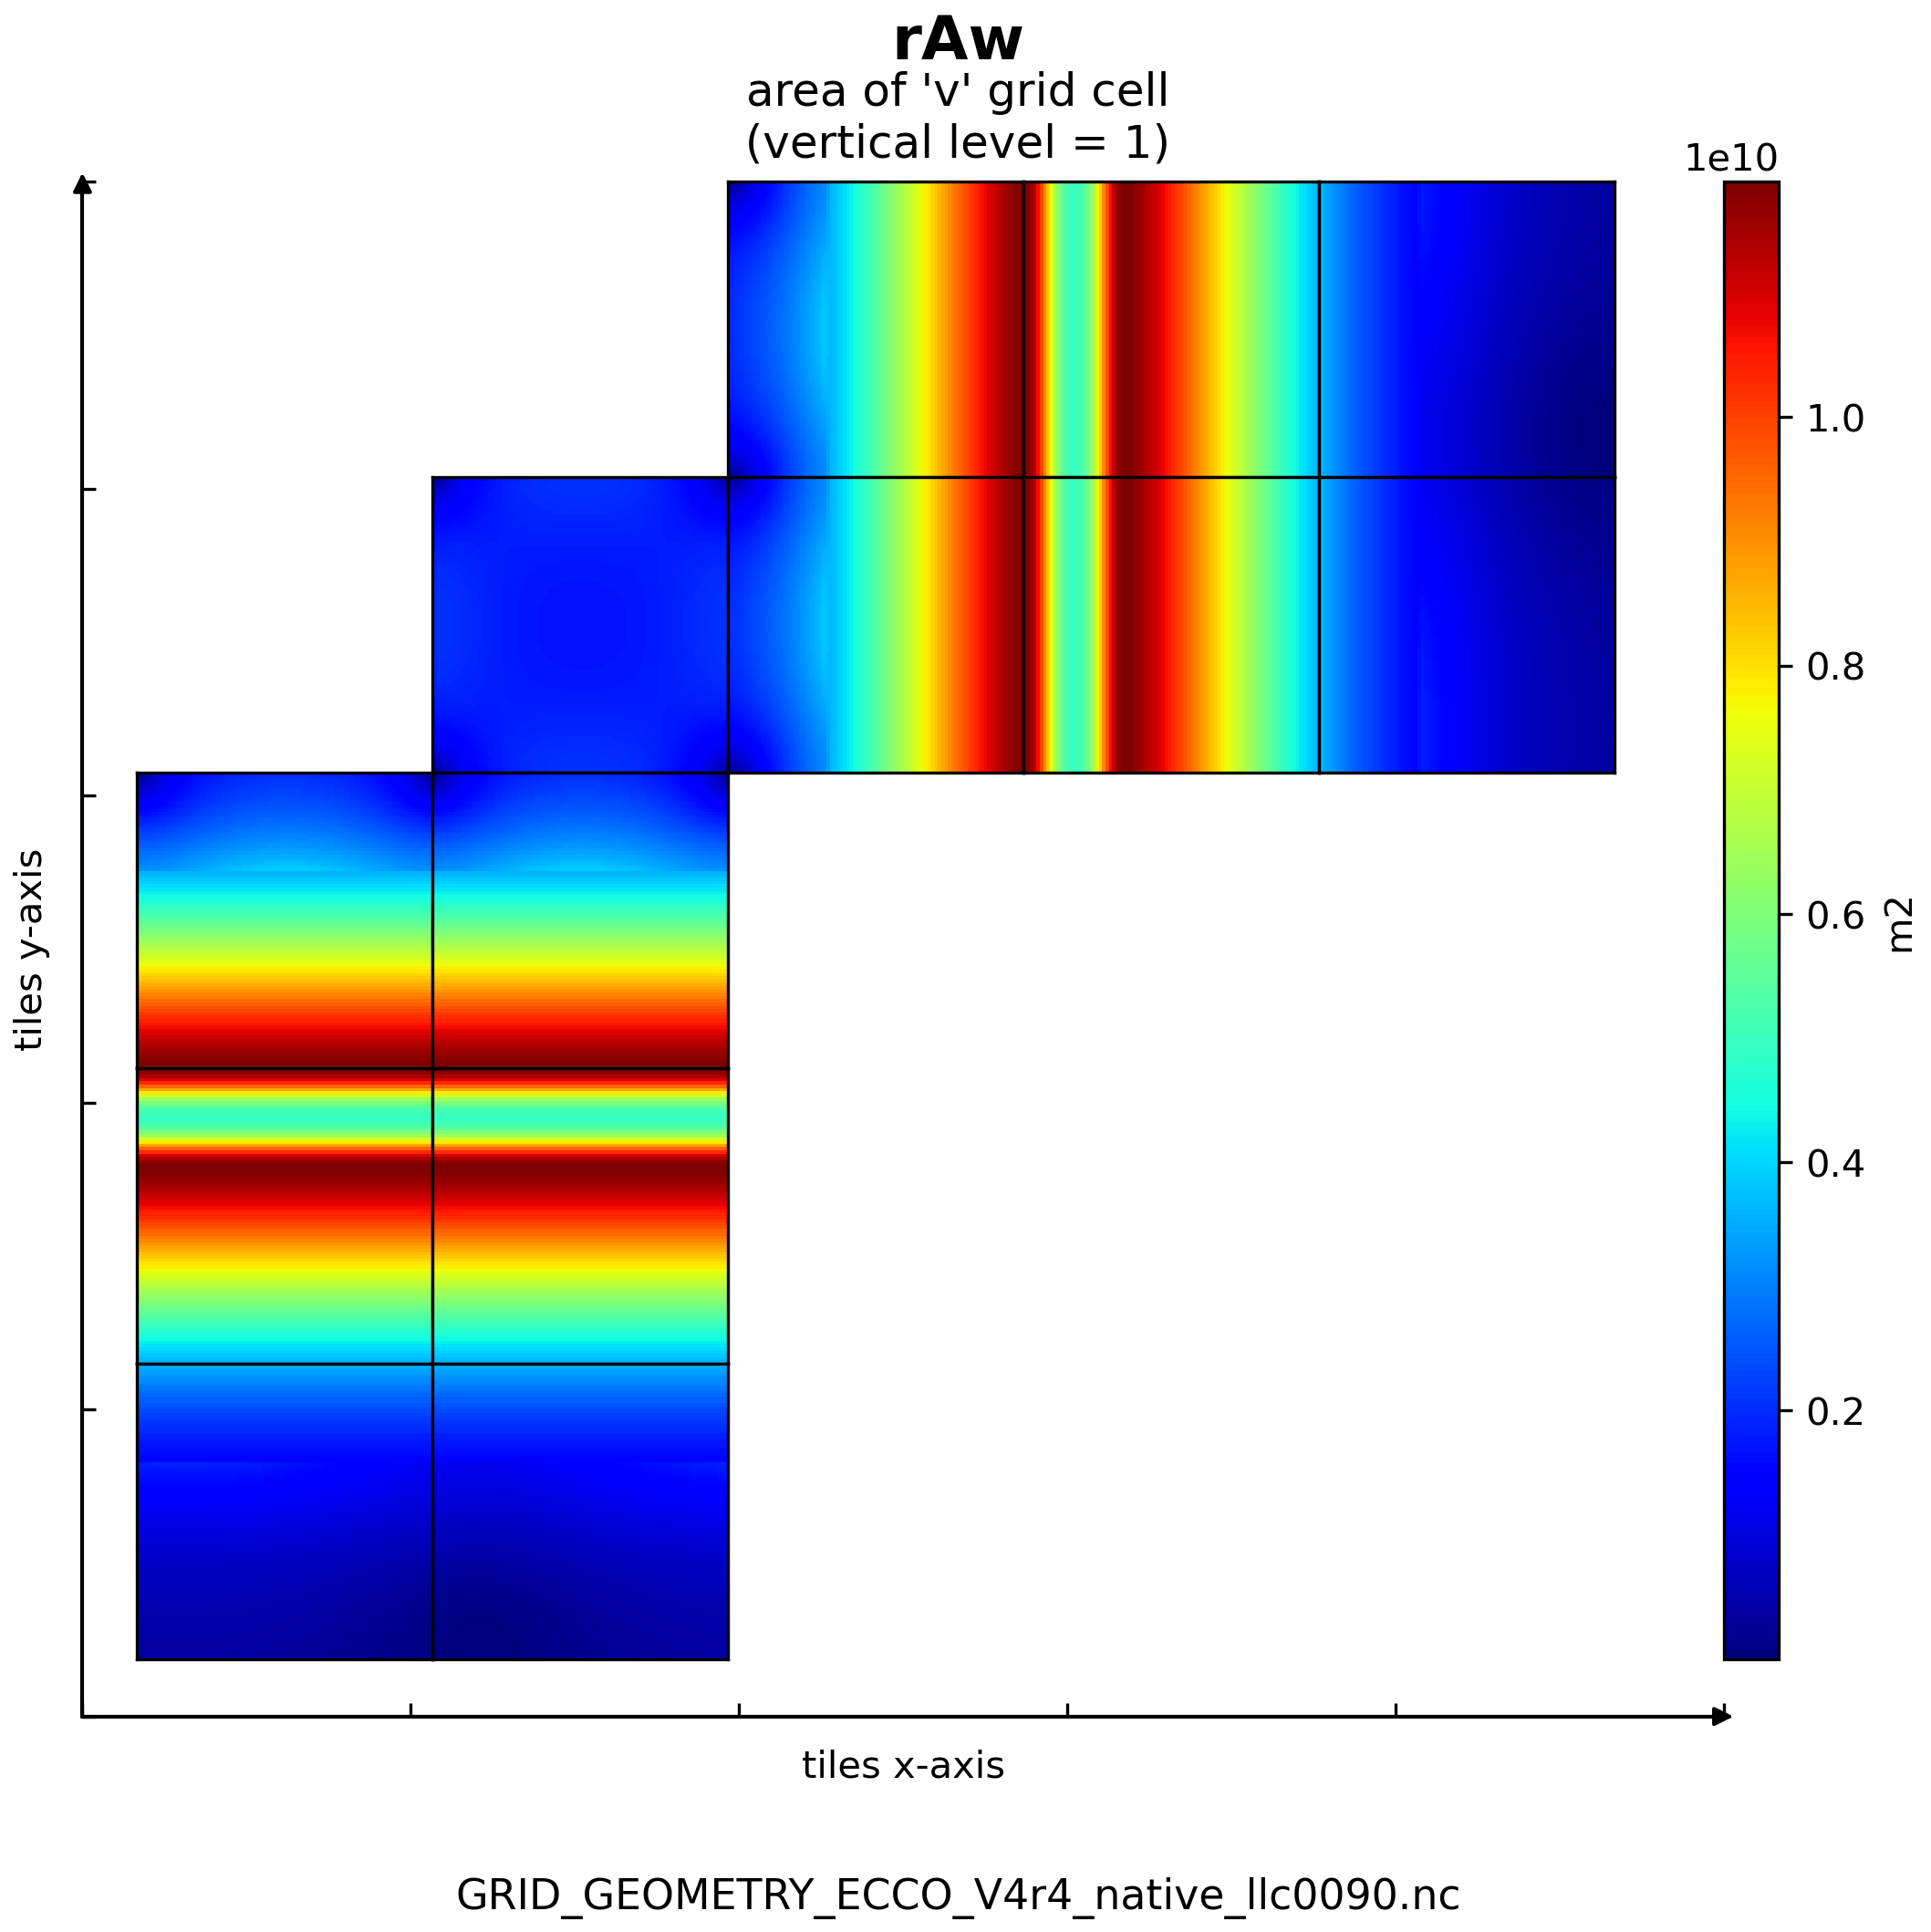
\includegraphics[scale=0.55]{../images/plots/v4r4/native_plots_coords/Geometry_Parameters_for_the_Lat-Lon-Cap_90_(llc90)_Native_Model_Grid_(Version_4_Release_4)/rAw.png}
\caption{Dataset: GRID\_GEOMETRY\_ECCO, Variable: rAw}
\label{tab:table-GRID_GEOMETRY_ECCO_rAw-Plot}
\end{figure}
\newpage
\pagebreak
\subsubsection{Native coordinates Variable: rAs}
\begin{longtable}{|m{0.06\textwidth}|m{0.3\textwidth}|m{0.45\textwidth}|m{0.12\textwidth}|}
\caption{Attributes description of the variable 'rAs' from GRID\_GEOMETRY\_ECCO's  dataset.}
\label{tab:table-GRID_GEOMETRY_ECCO_rAs} \\ 
\hline \endhead \hline \endfoot
\rowcolor{lightgray} \textbf{Storage Type} & \textbf{Variable Name} & \textbf{Description} & \textbf{Unit} \\ \hline
float32 & rAs & Area of 'u' grid cell & m2 \\ \hline
\multicolumn{4}{|c|}{\cellcolor{lightgray}{\textbf{Description of the variable in Common Data language (CDL)}}} \\ \hline
\multicolumn{4}{|c|}{\fontfamily{lmtt}\selectfont{\makecell{\parbox{.95\textwidth}{\vspace*{0.25cm} \footnotesize{float32 rAs(tile, j\_g, i)\\
\hspace*{0.5cm}rAs: \_FillValue = 9.96921e+36\\
\hspace*{0.5cm}rAs: coordinates = YG XC\\
\hspace*{0.5cm}rAs: coverage\_content\_type = modelResult\\
\hspace*{0.5cm}rAs: long\_name = area of u grid cell\\
\hspace*{0.5cm}rAs: standard\_name = cell area\\
\hspace*{0.5cm}rAs: units = m2\\
}}}}} \\ \hline
\rowcolor{lightgray} \multicolumn{4}{|c|}{\textbf{Comments}} \\ \hline
\multicolumn{4}{|p{1\textwidth}|}{\footnotesize{{Model 'u' grid cells are staggered in space between adjacent tracer grid cells in the 'y' direction. 'u' grid cell (i,j) is situated at the 'south' edge of tracer grid cell (i, j). note: 'south' does not correspond to geographic orientation but is used for convenience to describe the computational grid. see mitgcm documentation for details.}}} \\ \hline
\end{longtable}

\begin{figure}[H]
\centering
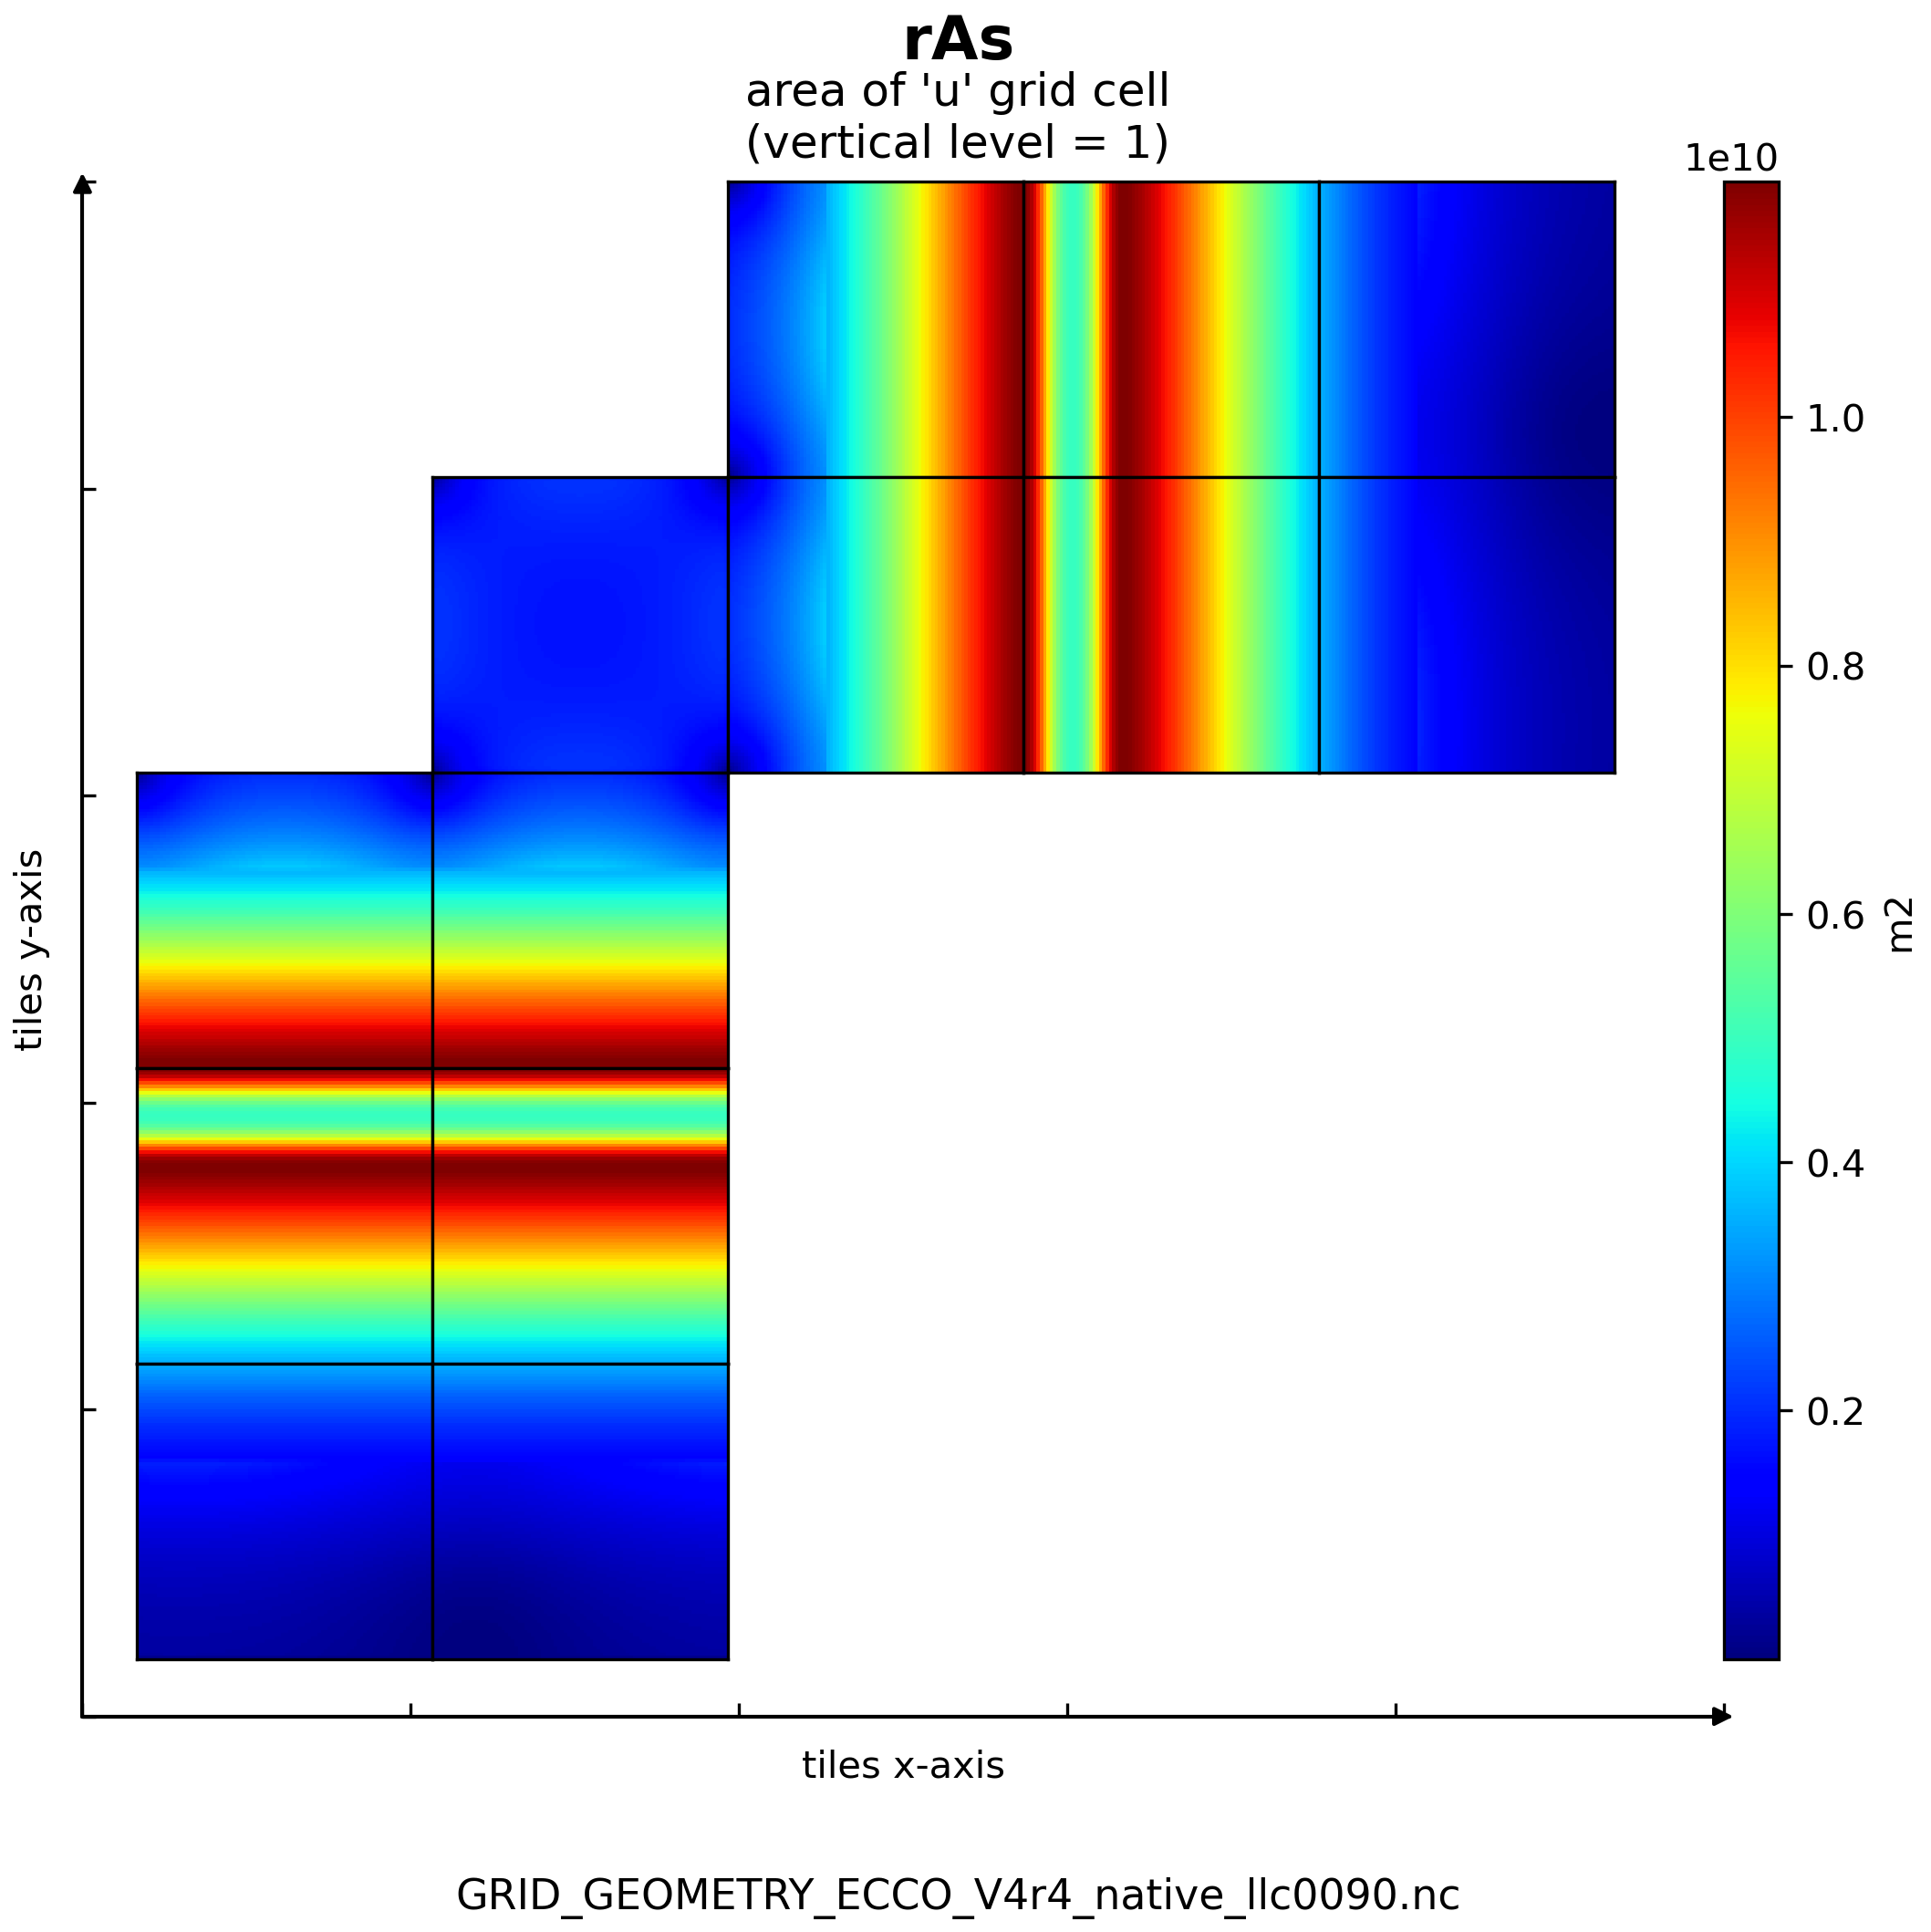
\includegraphics[scale=0.55]{../images/plots/v4r4/native_plots_coords/Geometry_Parameters_for_the_Lat-Lon-Cap_90_(llc90)_Native_Model_Grid_(Version_4_Release_4)/rAs.png}
\caption{Dataset: GRID\_GEOMETRY\_ECCO, Variable: rAs}
\label{tab:table-GRID_GEOMETRY_ECCO_rAs-Plot}
\end{figure}
\newpage
\pagebreak
\subsubsection{Native coordinates Variable: hFacC}
\begin{longtable}{|m{0.06\textwidth}|m{0.3\textwidth}|m{0.45\textwidth}|m{0.12\textwidth}|}
\caption{Attributes description of the variable 'hFacC' from GRID\_GEOMETRY\_ECCO's  dataset.}
\label{tab:table-GRID_GEOMETRY_ECCO_hFacC} \\ 
\hline \endhead \hline \endfoot
\rowcolor{lightgray} \textbf{Storage Type} & \textbf{Variable Name} & \textbf{Description} & \textbf{Unit} \\ \hline
float32 & hFacC & Vertical open fraction of tracer grid cell & 1 \\ \hline
\multicolumn{4}{|c|}{\cellcolor{lightgray}{\textbf{Description of the variable in Common Data language (CDL)}}} \\ \hline
\multicolumn{4}{|c|}{\fontfamily{lmtt}\selectfont{\makecell{\parbox{.95\textwidth}{\vspace*{0.25cm} \footnotesize{float32 hFacC(k, tile, j, i)\\
\hspace*{0.5cm}hFacC: \_FillValue = 9.96921e+36\\
\hspace*{0.5cm}hFacC: coordinates = Z YC XC\\
\hspace*{0.5cm}hFacC: coverage\_content\_type = modelResult\\
\hspace*{0.5cm}hFacC: long\_name = vertical open fraction of tracer grid cell\\
\hspace*{0.5cm}hFacC: units = 1\\
}}}}} \\ \hline
\rowcolor{lightgray} \multicolumn{4}{|c|}{\textbf{Comments}} \\ \hline
\multicolumn{4}{|p{1\textwidth}|}{\footnotesize{{Tracer grid cells may be fractionally closed in the vertical. the open vertical fraction is hfacc. the model allows for partially-filled cells to represent topographic variations more smoothly (hfacc < 1). completely closed (dry) tracer grid cells have hfacc = 0. note: the model z* coordinate system allows hfacc to vary through time. a time-invariant hfacc field is provided for reference.}}} \\ \hline
\end{longtable}

\begin{figure}[H]
\centering
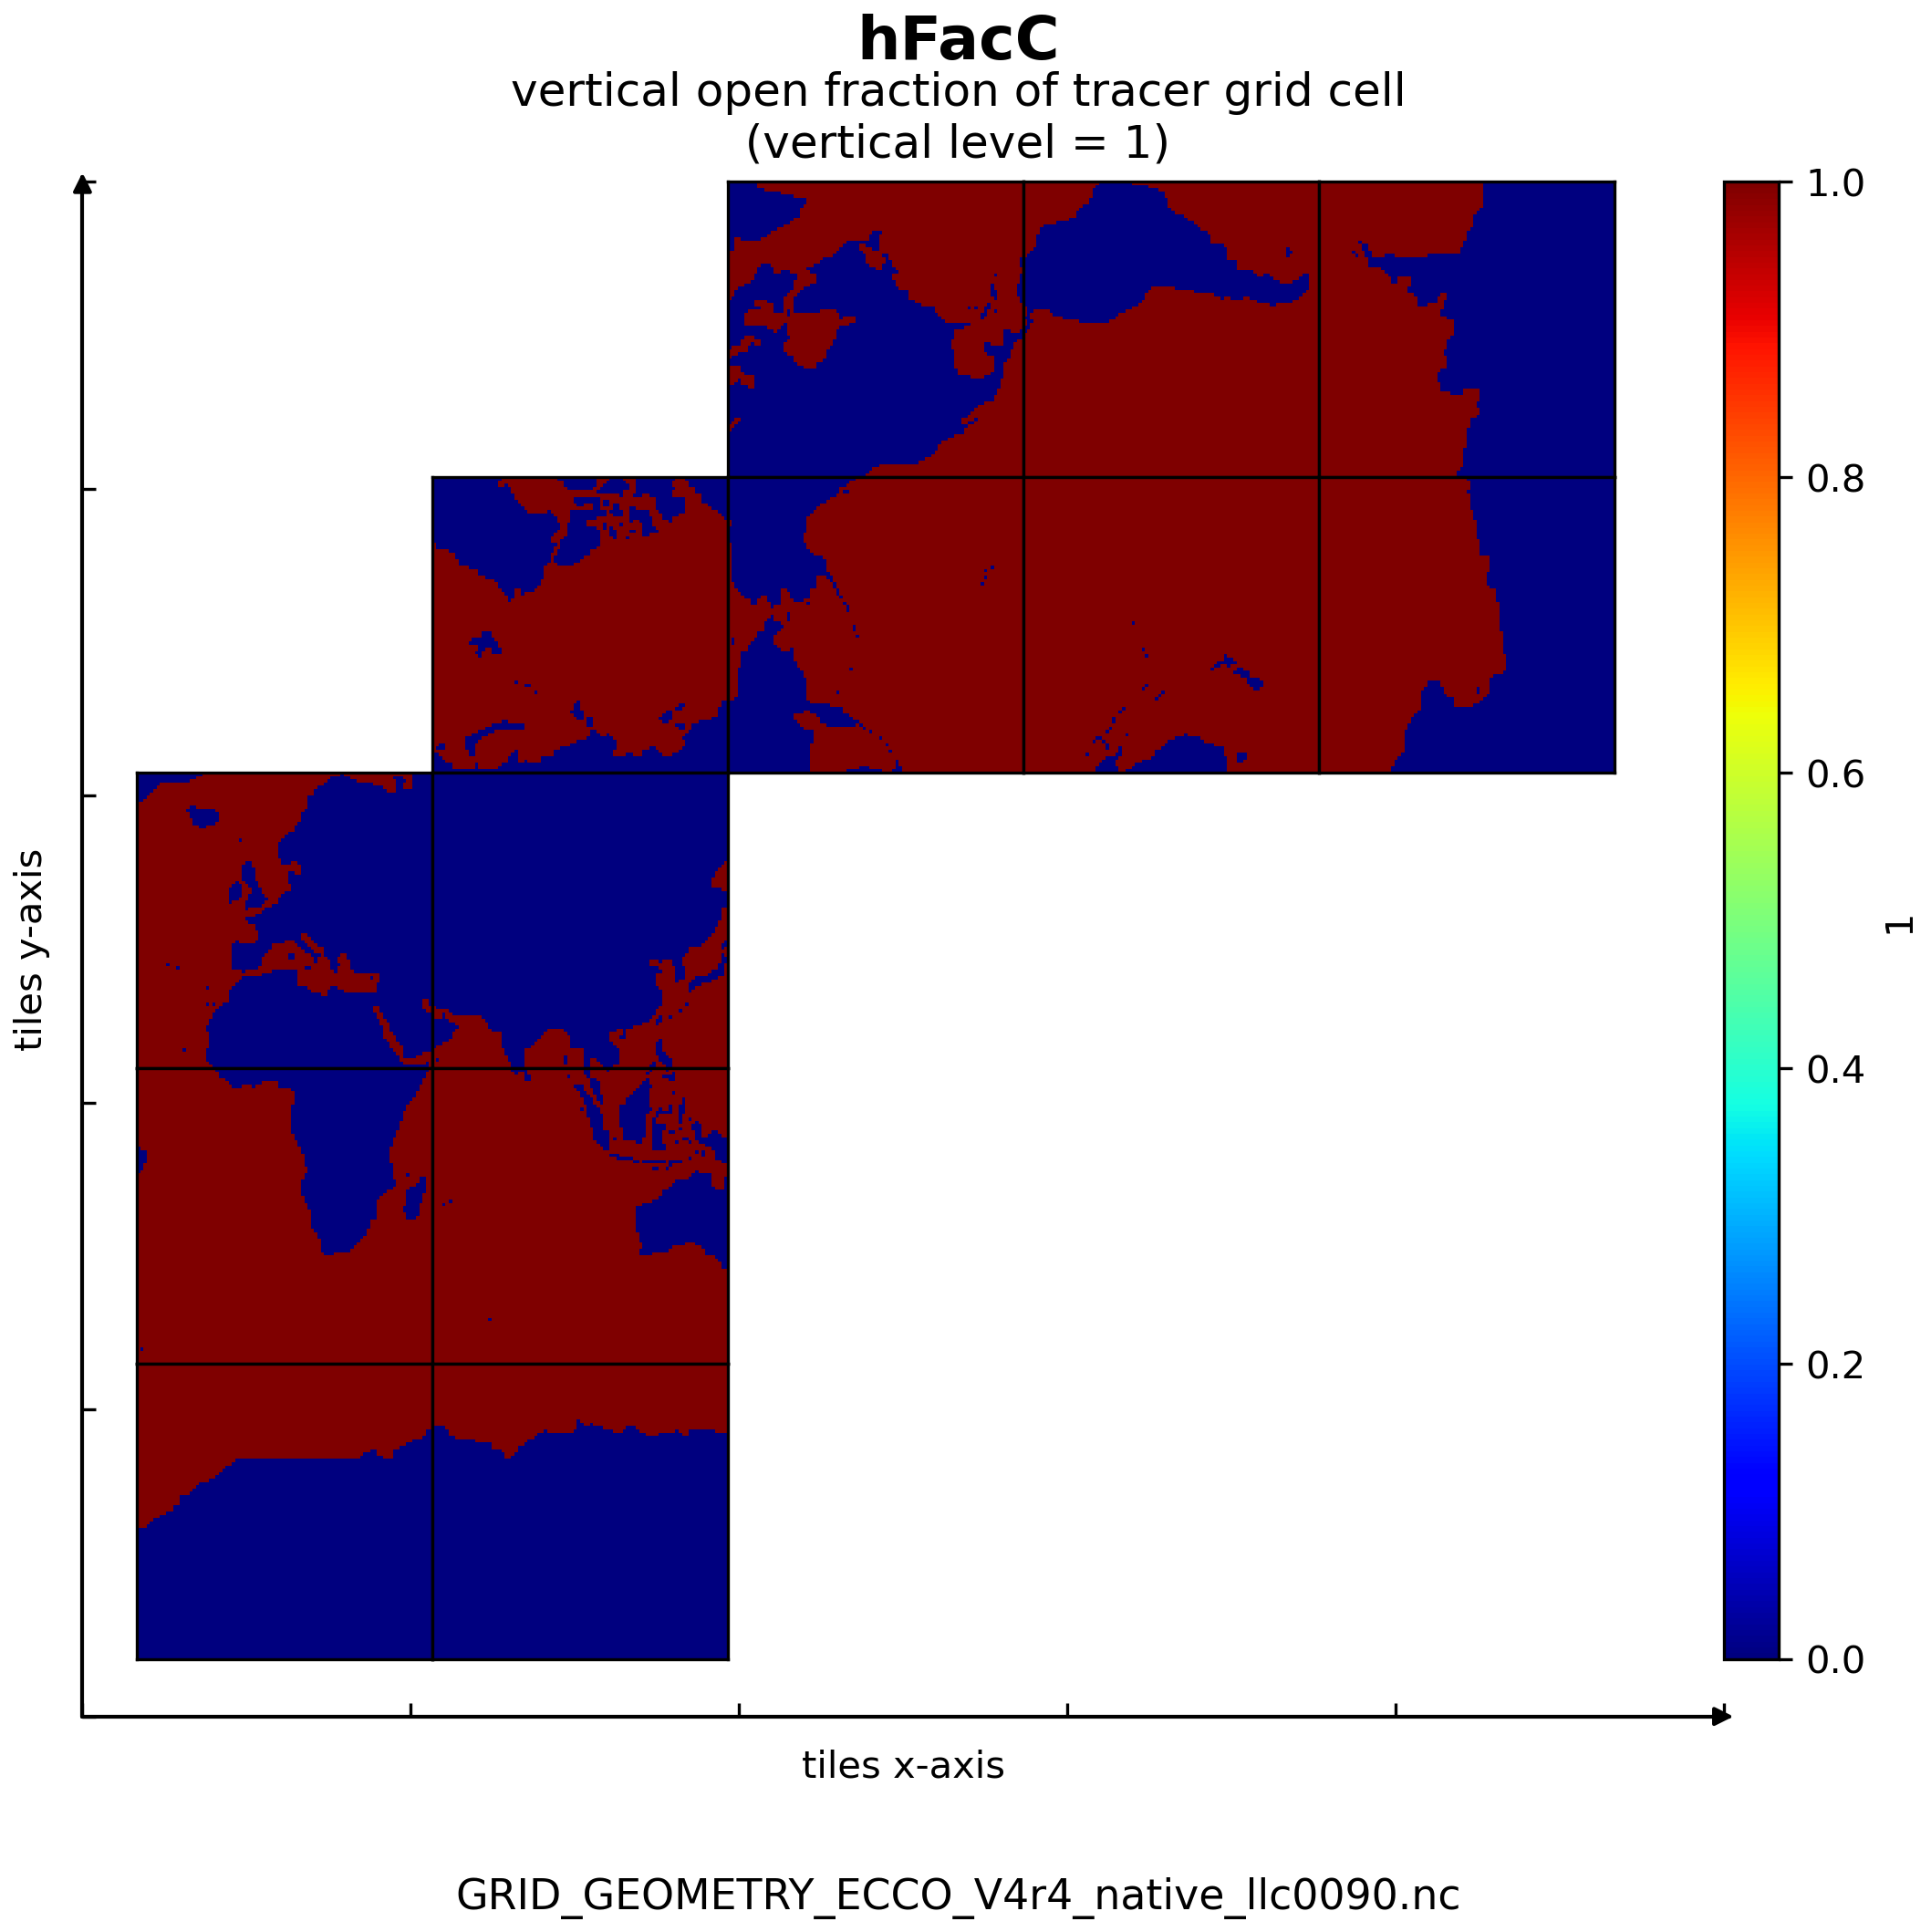
\includegraphics[scale=0.55]{../images/plots/v4r4/native_plots_coords/Geometry_Parameters_for_the_Lat-Lon-Cap_90_(llc90)_Native_Model_Grid_(Version_4_Release_4)/hFacC.png}
\caption{Dataset: GRID\_GEOMETRY\_ECCO, Variable: hFacC}
\label{tab:table-GRID_GEOMETRY_ECCO_hFacC-Plot}
\end{figure}
\newpage
\pagebreak
\subsubsection{Native coordinates Variable: hFacW}
\begin{longtable}{|m{0.06\textwidth}|m{0.3\textwidth}|m{0.45\textwidth}|m{0.12\textwidth}|}
\caption{Attributes description of the variable 'hFacW' from GRID\_GEOMETRY\_ECCO's  dataset.}
\label{tab:table-GRID_GEOMETRY_ECCO_hFacW} \\ 
\hline \endhead \hline \endfoot
\rowcolor{lightgray} \textbf{Storage Type} & \textbf{Variable Name} & \textbf{Description} & \textbf{Unit} \\ \hline
float32 & hFacW & Vertical open fraction of tracer grid cell 'west' face & 1 \\ \hline
\multicolumn{4}{|c|}{\cellcolor{lightgray}{\textbf{Description of the variable in Common Data language (CDL)}}} \\ \hline
\multicolumn{4}{|c|}{\fontfamily{lmtt}\selectfont{\makecell{\parbox{.95\textwidth}{\vspace*{0.25cm} \footnotesize{float32 hFacW(k, tile, j, i\_g)\\
\hspace*{0.5cm}hFacW: \_FillValue = 9.96921e+36\\
\hspace*{0.5cm}hFacW: coordinates = Z\\
\hspace*{0.5cm}hFacW: coverage\_content\_type = modelResult\\
\hspace*{0.5cm}hFacW: long\_name = vertical open fraction of tracer grid cell west face\\
\hspace*{0.5cm}hFacW: units = 1\\
}}}}} \\ \hline
\rowcolor{lightgray} \multicolumn{4}{|c|}{\textbf{Comments}} \\ \hline
\multicolumn{4}{|p{1\textwidth}|}{\footnotesize{{The 'west' face of tracer grid cells may be fractionally closed in the vertical. the open vertical fraction is hfacw. the model allows for partially-filled cells for smoother representation of seafloor topography. tracer grid cells adjacent in the 'x' direction that are partially closed in the vertical have hfacw < 1. the model z* coordinate system used by the model permits hfacc, and therefore hfacw, to vary through time. a time-invariant hfacw field is provided for reference. note: the term 'west' does not correspond to geographic orientation but is used for convenience to describe the computational grid. see mitgcm documentation for details.}}} \\ \hline
\end{longtable}

\begin{figure}[H]
\centering
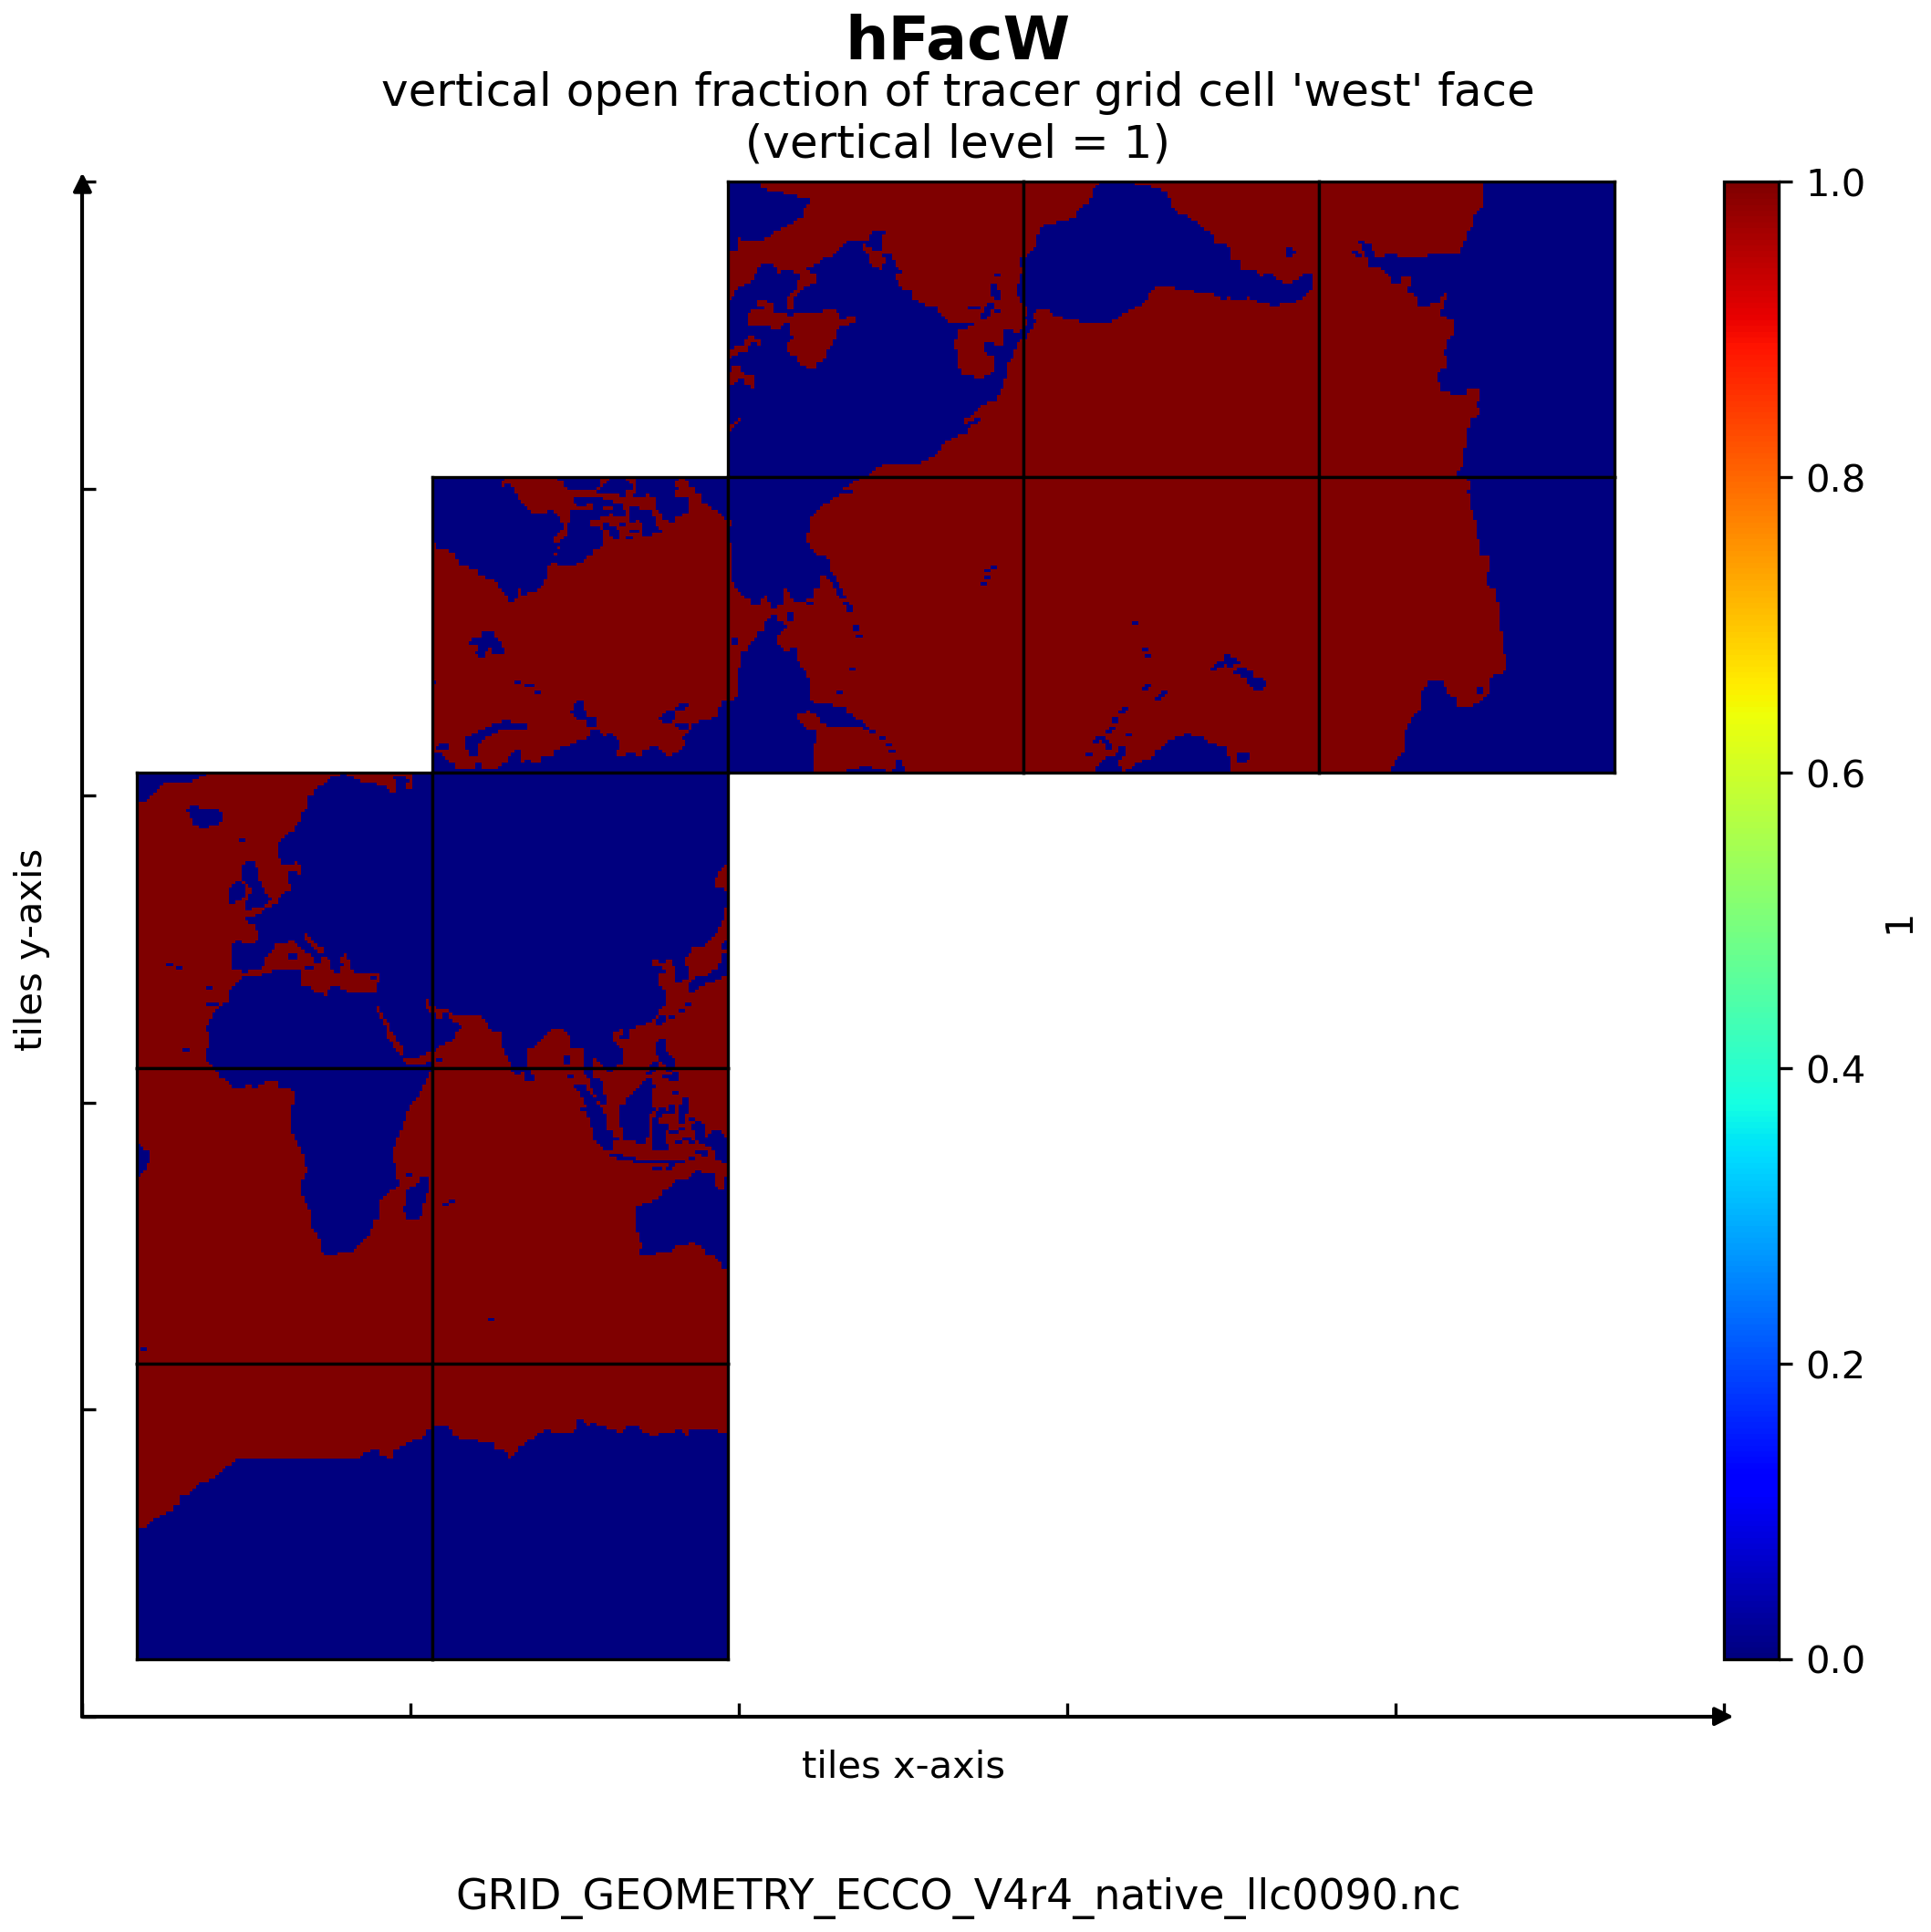
\includegraphics[scale=0.55]{../images/plots/v4r4/native_plots_coords/Geometry_Parameters_for_the_Lat-Lon-Cap_90_(llc90)_Native_Model_Grid_(Version_4_Release_4)/hFacW.png}
\caption{Dataset: GRID\_GEOMETRY\_ECCO, Variable: hFacW}
\label{tab:table-GRID_GEOMETRY_ECCO_hFacW-Plot}
\end{figure}
\newpage
\pagebreak
\subsubsection{Native coordinates Variable: hFacS}
\begin{longtable}{|m{0.06\textwidth}|m{0.3\textwidth}|m{0.45\textwidth}|m{0.12\textwidth}|}
\caption{Attributes description of the variable 'hFacS' from GRID\_GEOMETRY\_ECCO's  dataset.}
\label{tab:table-GRID_GEOMETRY_ECCO_hFacS} \\ 
\hline \endhead \hline \endfoot
\rowcolor{lightgray} \textbf{Storage Type} & \textbf{Variable Name} & \textbf{Description} & \textbf{Unit} \\ \hline
float32 & hFacS & Vertical open fraction of tracer grid cell 'south' face & 1 \\ \hline
\multicolumn{4}{|c|}{\cellcolor{lightgray}{\textbf{Description of the variable in Common Data language (CDL)}}} \\ \hline
\multicolumn{4}{|c|}{\fontfamily{lmtt}\selectfont{\makecell{\parbox{.95\textwidth}{\vspace*{0.25cm} \footnotesize{float32 hFacS(k, tile, j\_g, i)\\
\hspace*{0.5cm}hFacS: \_FillValue = 9.96921e+36\\
\hspace*{0.5cm}hFacS: coordinates = Z\\
\hspace*{0.5cm}hFacS: coverage\_content\_type = modelResult\\
\hspace*{0.5cm}hFacS: long\_name = vertical open fraction of tracer grid cell south face\\
\hspace*{0.5cm}hFacS: units = 1\\
}}}}} \\ \hline
\rowcolor{lightgray} \multicolumn{4}{|c|}{\textbf{Comments}} \\ \hline
\multicolumn{4}{|p{1\textwidth}|}{\footnotesize{{The 'south' face of tracer grid cells may be fractionally closed in the vertical. the open vertical fraction is hfacs. the model allows for partially-filled cells for smoother representation of seafloor topography. tracer grid cells adjacent in the 'y' direction that are partially closed in the vertical have hfacs < 1. the model z* coordinate system used by the model permits hfacc, and therefore hfacs, to vary through time. a time-invariant hfacs field is provided for reference. note:  the term 'south' does not correspond to geographic orientation but is used for convenience to describe the computational grid. see mitgcm documentation for details.}}} \\ \hline
\end{longtable}

\begin{figure}[H]
\centering
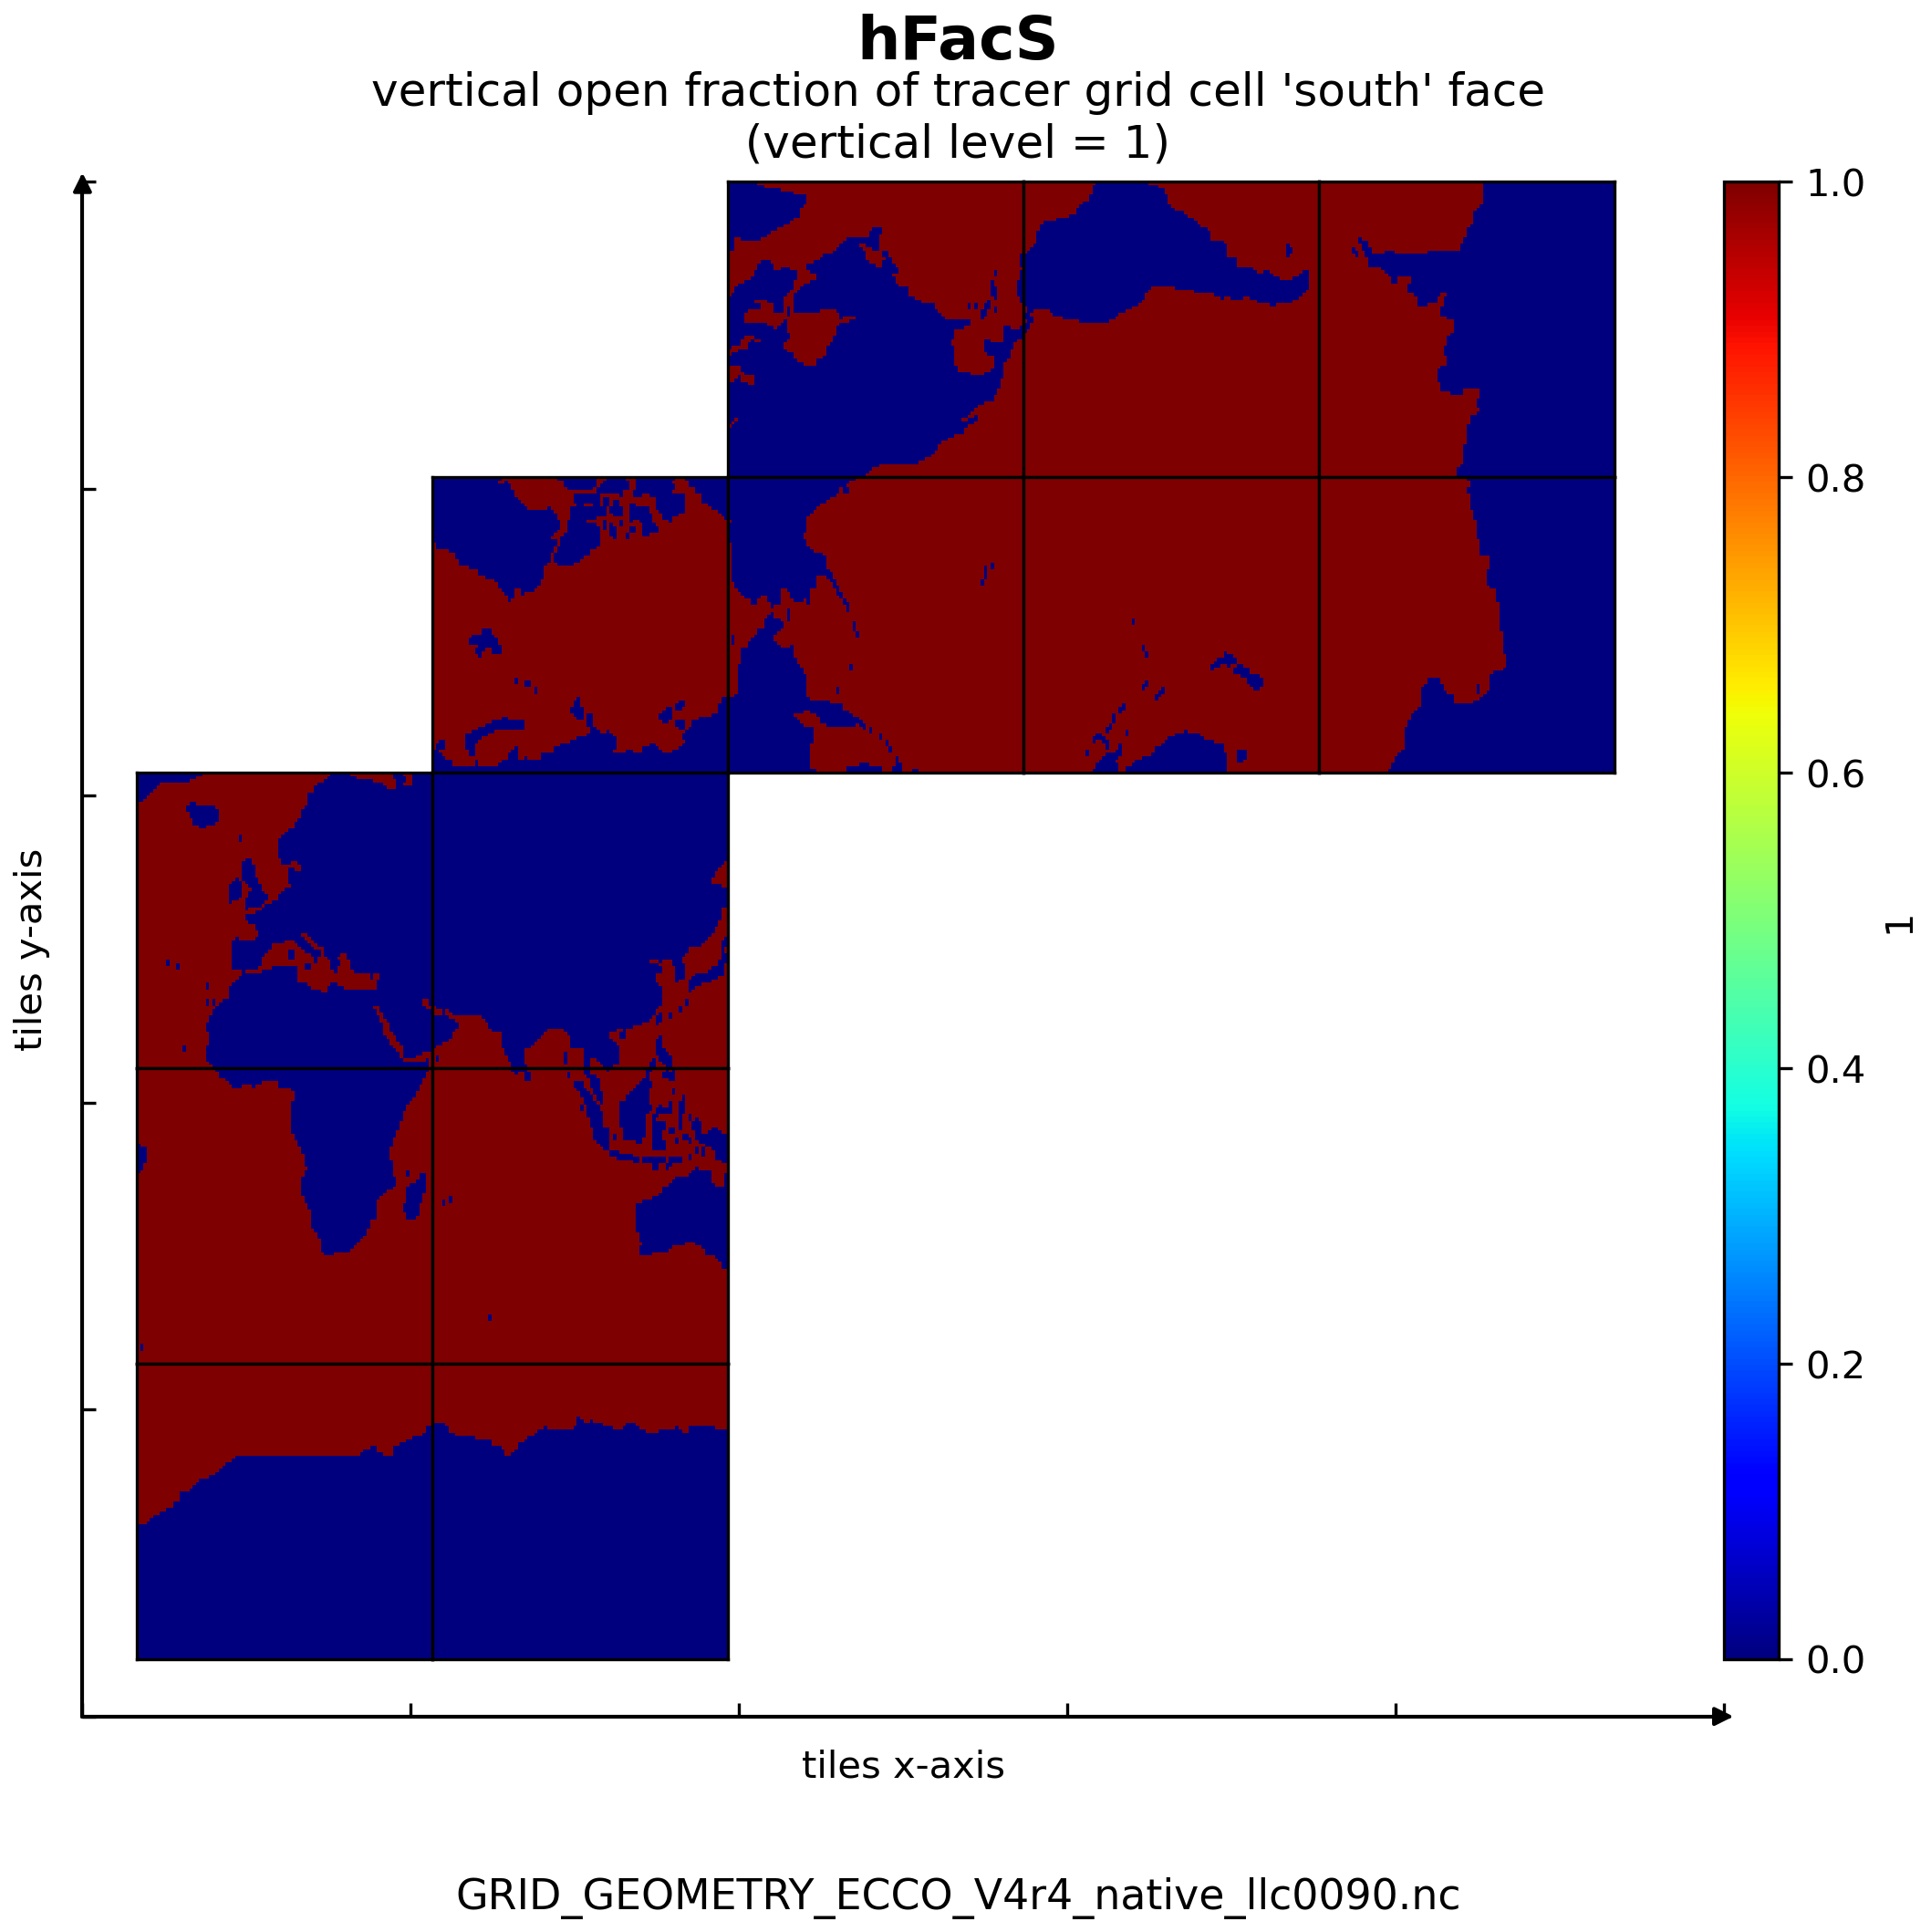
\includegraphics[scale=0.55]{../images/plots/v4r4/native_plots_coords/Geometry_Parameters_for_the_Lat-Lon-Cap_90_(llc90)_Native_Model_Grid_(Version_4_Release_4)/hFacS.png}
\caption{Dataset: GRID\_GEOMETRY\_ECCO, Variable: hFacS}
\label{tab:table-GRID_GEOMETRY_ECCO_hFacS-Plot}
\end{figure}
\newpage
\pagebreak
\subsubsection{Native coordinates Variable: maskC}
\begin{longtable}{|m{0.06\textwidth}|m{0.3\textwidth}|m{0.45\textwidth}|m{0.12\textwidth}|}
\caption{Attributes description of the variable 'maskC' from GRID\_GEOMETRY\_ECCO's  dataset.}
\label{tab:table-GRID_GEOMETRY_ECCO_maskC} \\ 
\hline \endhead \hline \endfoot
\rowcolor{lightgray} \textbf{Storage Type} & \textbf{Variable Name} & \textbf{Description} & \textbf{Unit} \\ \hline
bool & maskC & Wet/dry boolean mask for tracer grid cell & N/A \\ \hline
\multicolumn{4}{|c|}{\cellcolor{lightgray}{\textbf{Description of the variable in Common Data language (CDL)}}} \\ \hline
\multicolumn{4}{|c|}{\fontfamily{lmtt}\selectfont{\makecell{\parbox{.95\textwidth}{\vspace*{0.25cm} \footnotesize{bool maskC(k, tile, j, i)\\
\hspace*{0.5cm}maskC: \_FillValue = 1\\
\hspace*{0.5cm}maskC: coordinates = Z YC XC\\
\hspace*{0.5cm}maskC: coverage\_content\_type = modelResult\\
\hspace*{0.5cm}maskC: long\_name = wet/dry boolean mask for tracer grid cell\\
}}}}} \\ \hline
\rowcolor{lightgray} \multicolumn{4}{|c|}{\textbf{Comments}} \\ \hline
\multicolumn{4}{|p{1\textwidth}|}{\footnotesize{{True for tracer grid cells with nonzero open vertical fraction (hfacc > 0), otherwise false. although hfacc can vary though time, cells will never close if starting open and will never open if starting closed: hfacc(i,j,k,t) > 0 for all t, if hfacc(i,j,k,t=0) and hfacc(i,j,k,t) = 0 for all t, if hfacc(i,j,k,t=0) = 0. therefore, maskc is time invariant.}}} \\ \hline
\end{longtable}

\begin{figure}[H]
\centering
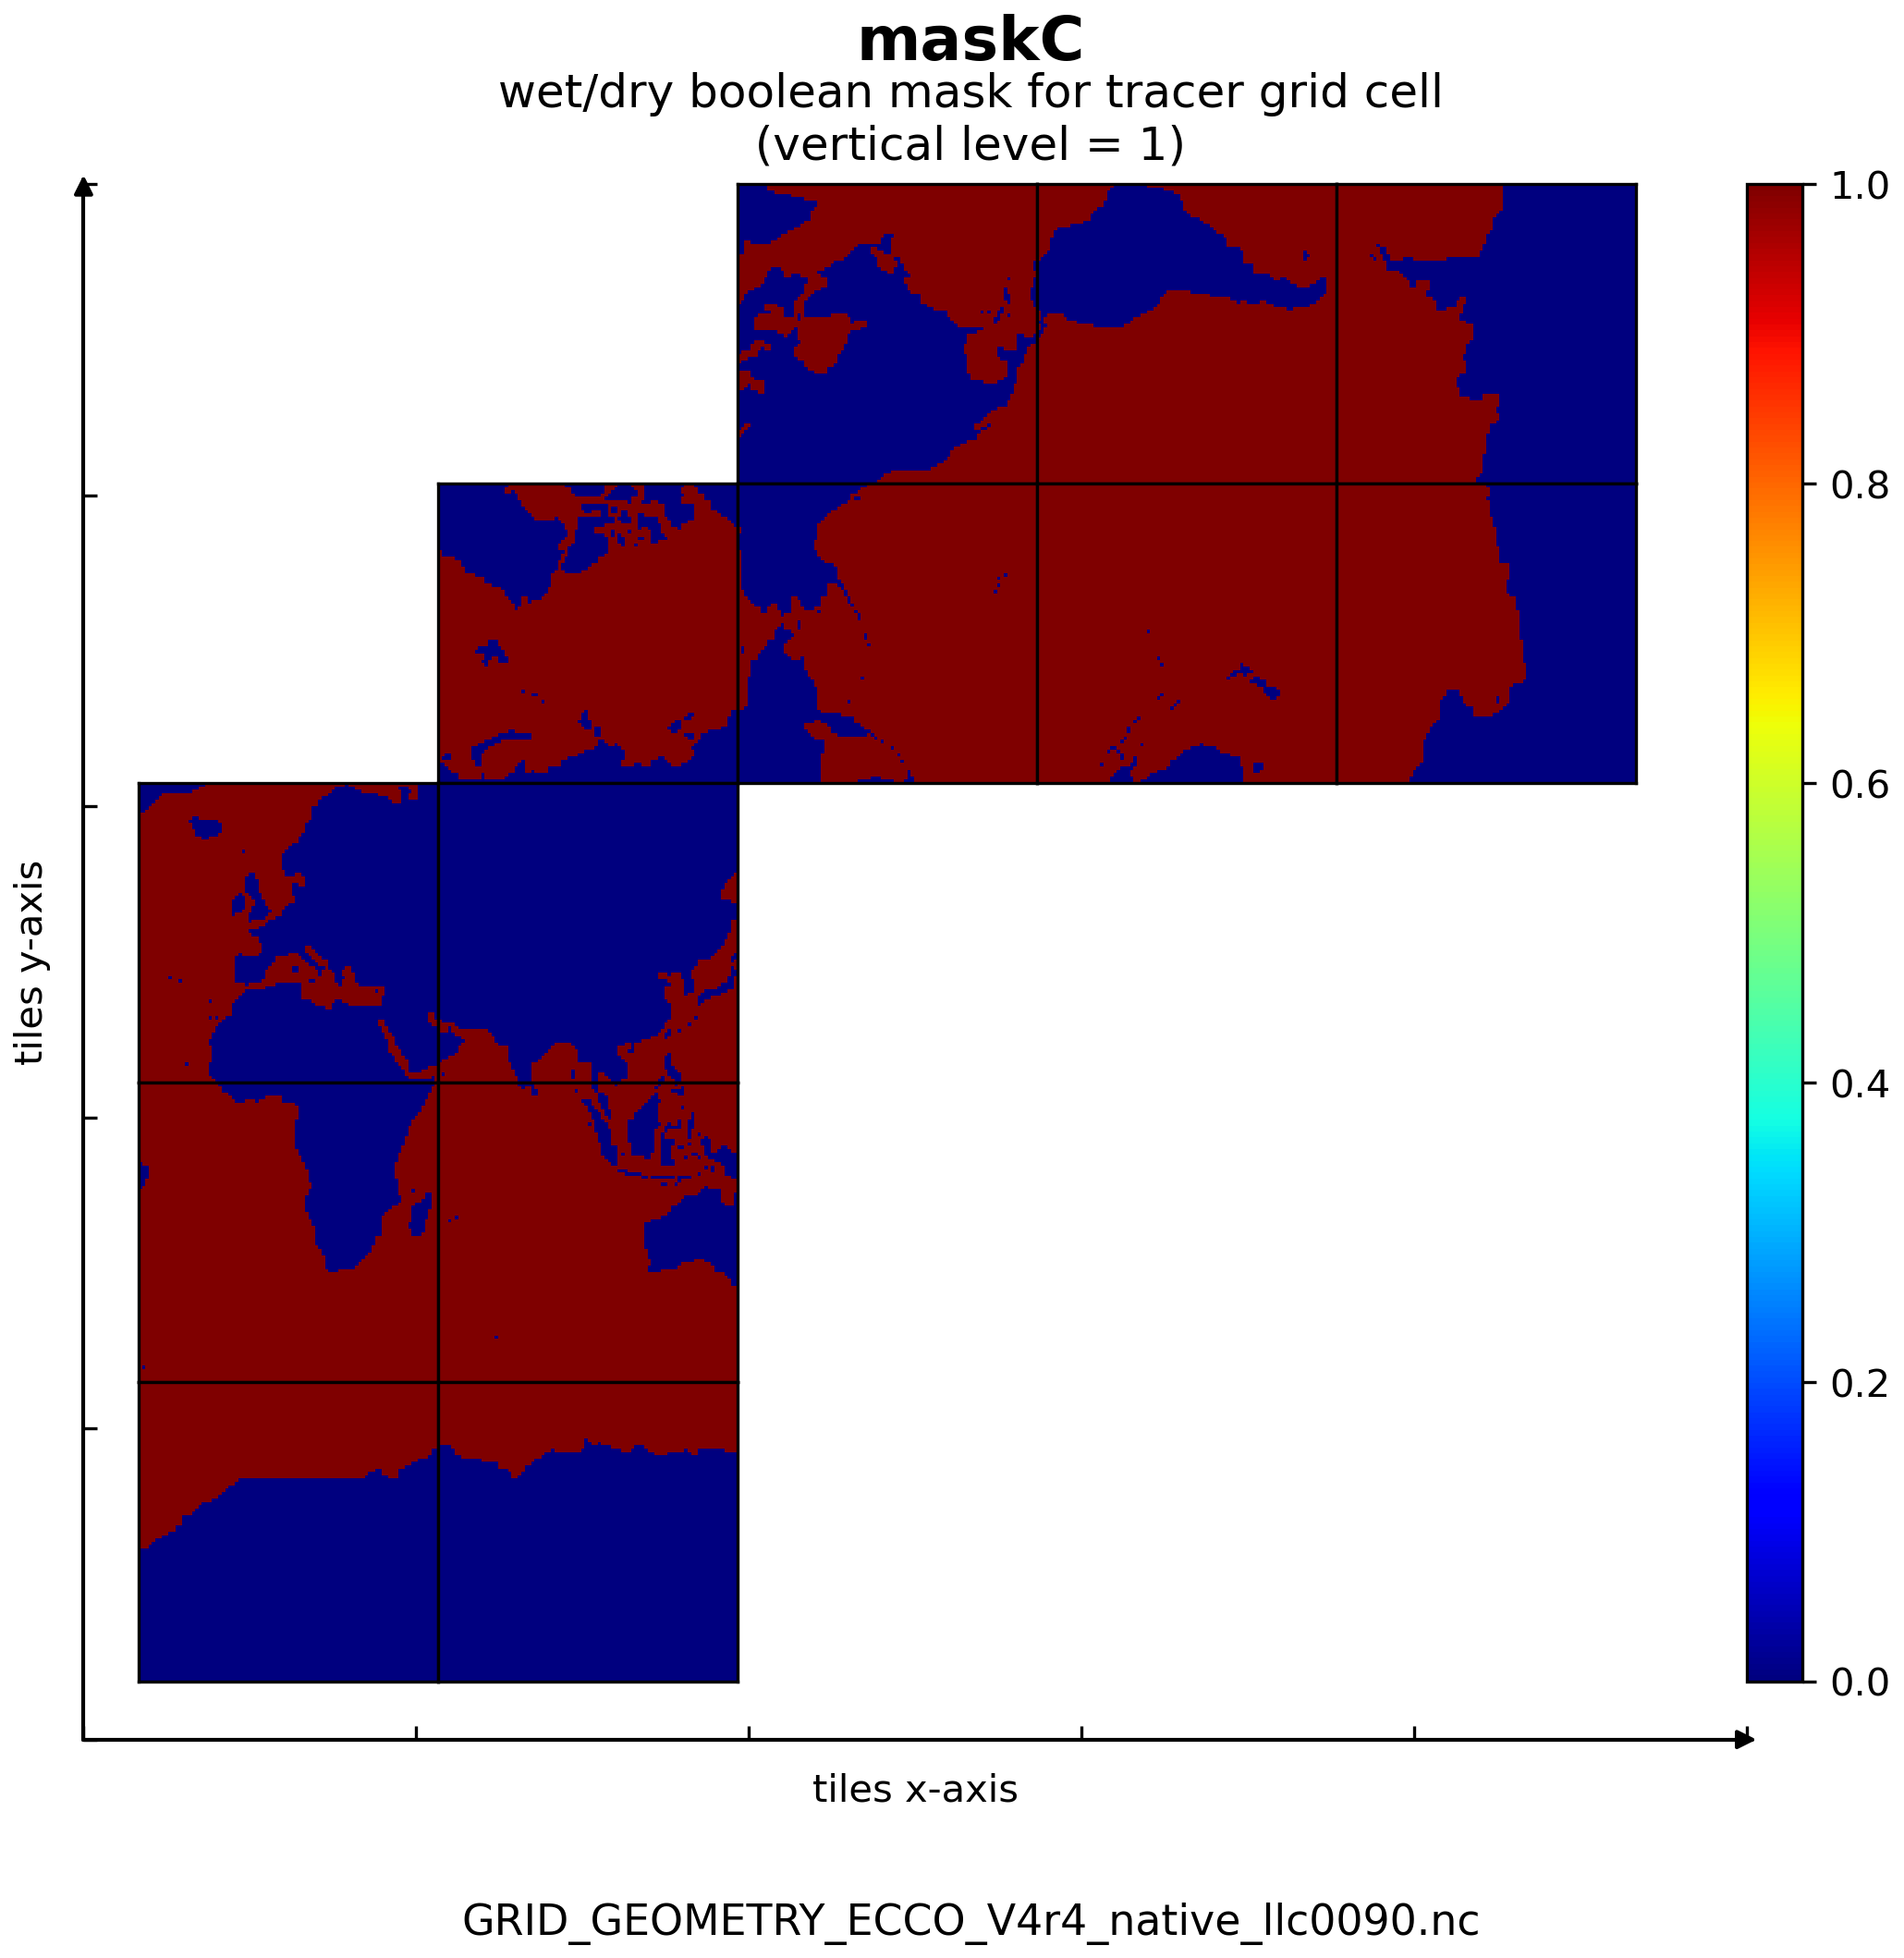
\includegraphics[scale=0.55]{../images/plots/v4r4/native_plots_coords/Geometry_Parameters_for_the_Lat-Lon-Cap_90_(llc90)_Native_Model_Grid_(Version_4_Release_4)/maskC.png}
\caption{Dataset: GRID\_GEOMETRY\_ECCO, Variable: maskC}
\label{tab:table-GRID_GEOMETRY_ECCO_maskC-Plot}
\end{figure}
\newpage
\pagebreak
\subsubsection{Native coordinates Variable: maskW}
\begin{longtable}{|m{0.06\textwidth}|m{0.3\textwidth}|m{0.45\textwidth}|m{0.12\textwidth}|}
\caption{Attributes description of the variable 'maskW' from GRID\_GEOMETRY\_ECCO's  dataset.}
\label{tab:table-GRID_GEOMETRY_ECCO_maskW} \\ 
\hline \endhead \hline \endfoot
\rowcolor{lightgray} \textbf{Storage Type} & \textbf{Variable Name} & \textbf{Description} & \textbf{Unit} \\ \hline
bool & maskW & Wet/dry boolean mask for 'west' face of tracer grid cell & N/A \\ \hline
\multicolumn{4}{|c|}{\cellcolor{lightgray}{\textbf{Description of the variable in Common Data language (CDL)}}} \\ \hline
\multicolumn{4}{|c|}{\fontfamily{lmtt}\selectfont{\makecell{\parbox{.95\textwidth}{\vspace*{0.25cm} \footnotesize{bool maskW(k, tile, j, i\_g)\\
\hspace*{0.5cm}maskW: \_FillValue = 1\\
\hspace*{0.5cm}maskW: coordinates = Z\\
\hspace*{0.5cm}maskW: coverage\_content\_type = modelResult\\
\hspace*{0.5cm}maskW: long\_name = wet/dry boolean mask for west face of tracer grid cell\\
}}}}} \\ \hline
\rowcolor{lightgray} \multicolumn{4}{|c|}{\textbf{Comments}} \\ \hline
\multicolumn{4}{|p{1\textwidth}|}{\footnotesize{{True for grid cells with nonzero open vertical fraction along their 'west' face (hfacw > 0), otherwise false. although hfacw can vary though time, cells will never close if starting open and will never open if starting closed: hfacw(i,j,k,t) > 0 for all t, if hfacw(i,j,k,t=0) and hfacw(i,j,k,t) = 0 for all t, if hfacw(i,j,k,t=0) = 0. therefore, maskw is time invariant. note: }}} \\ \hline
\end{longtable}

\begin{figure}[H]
\centering
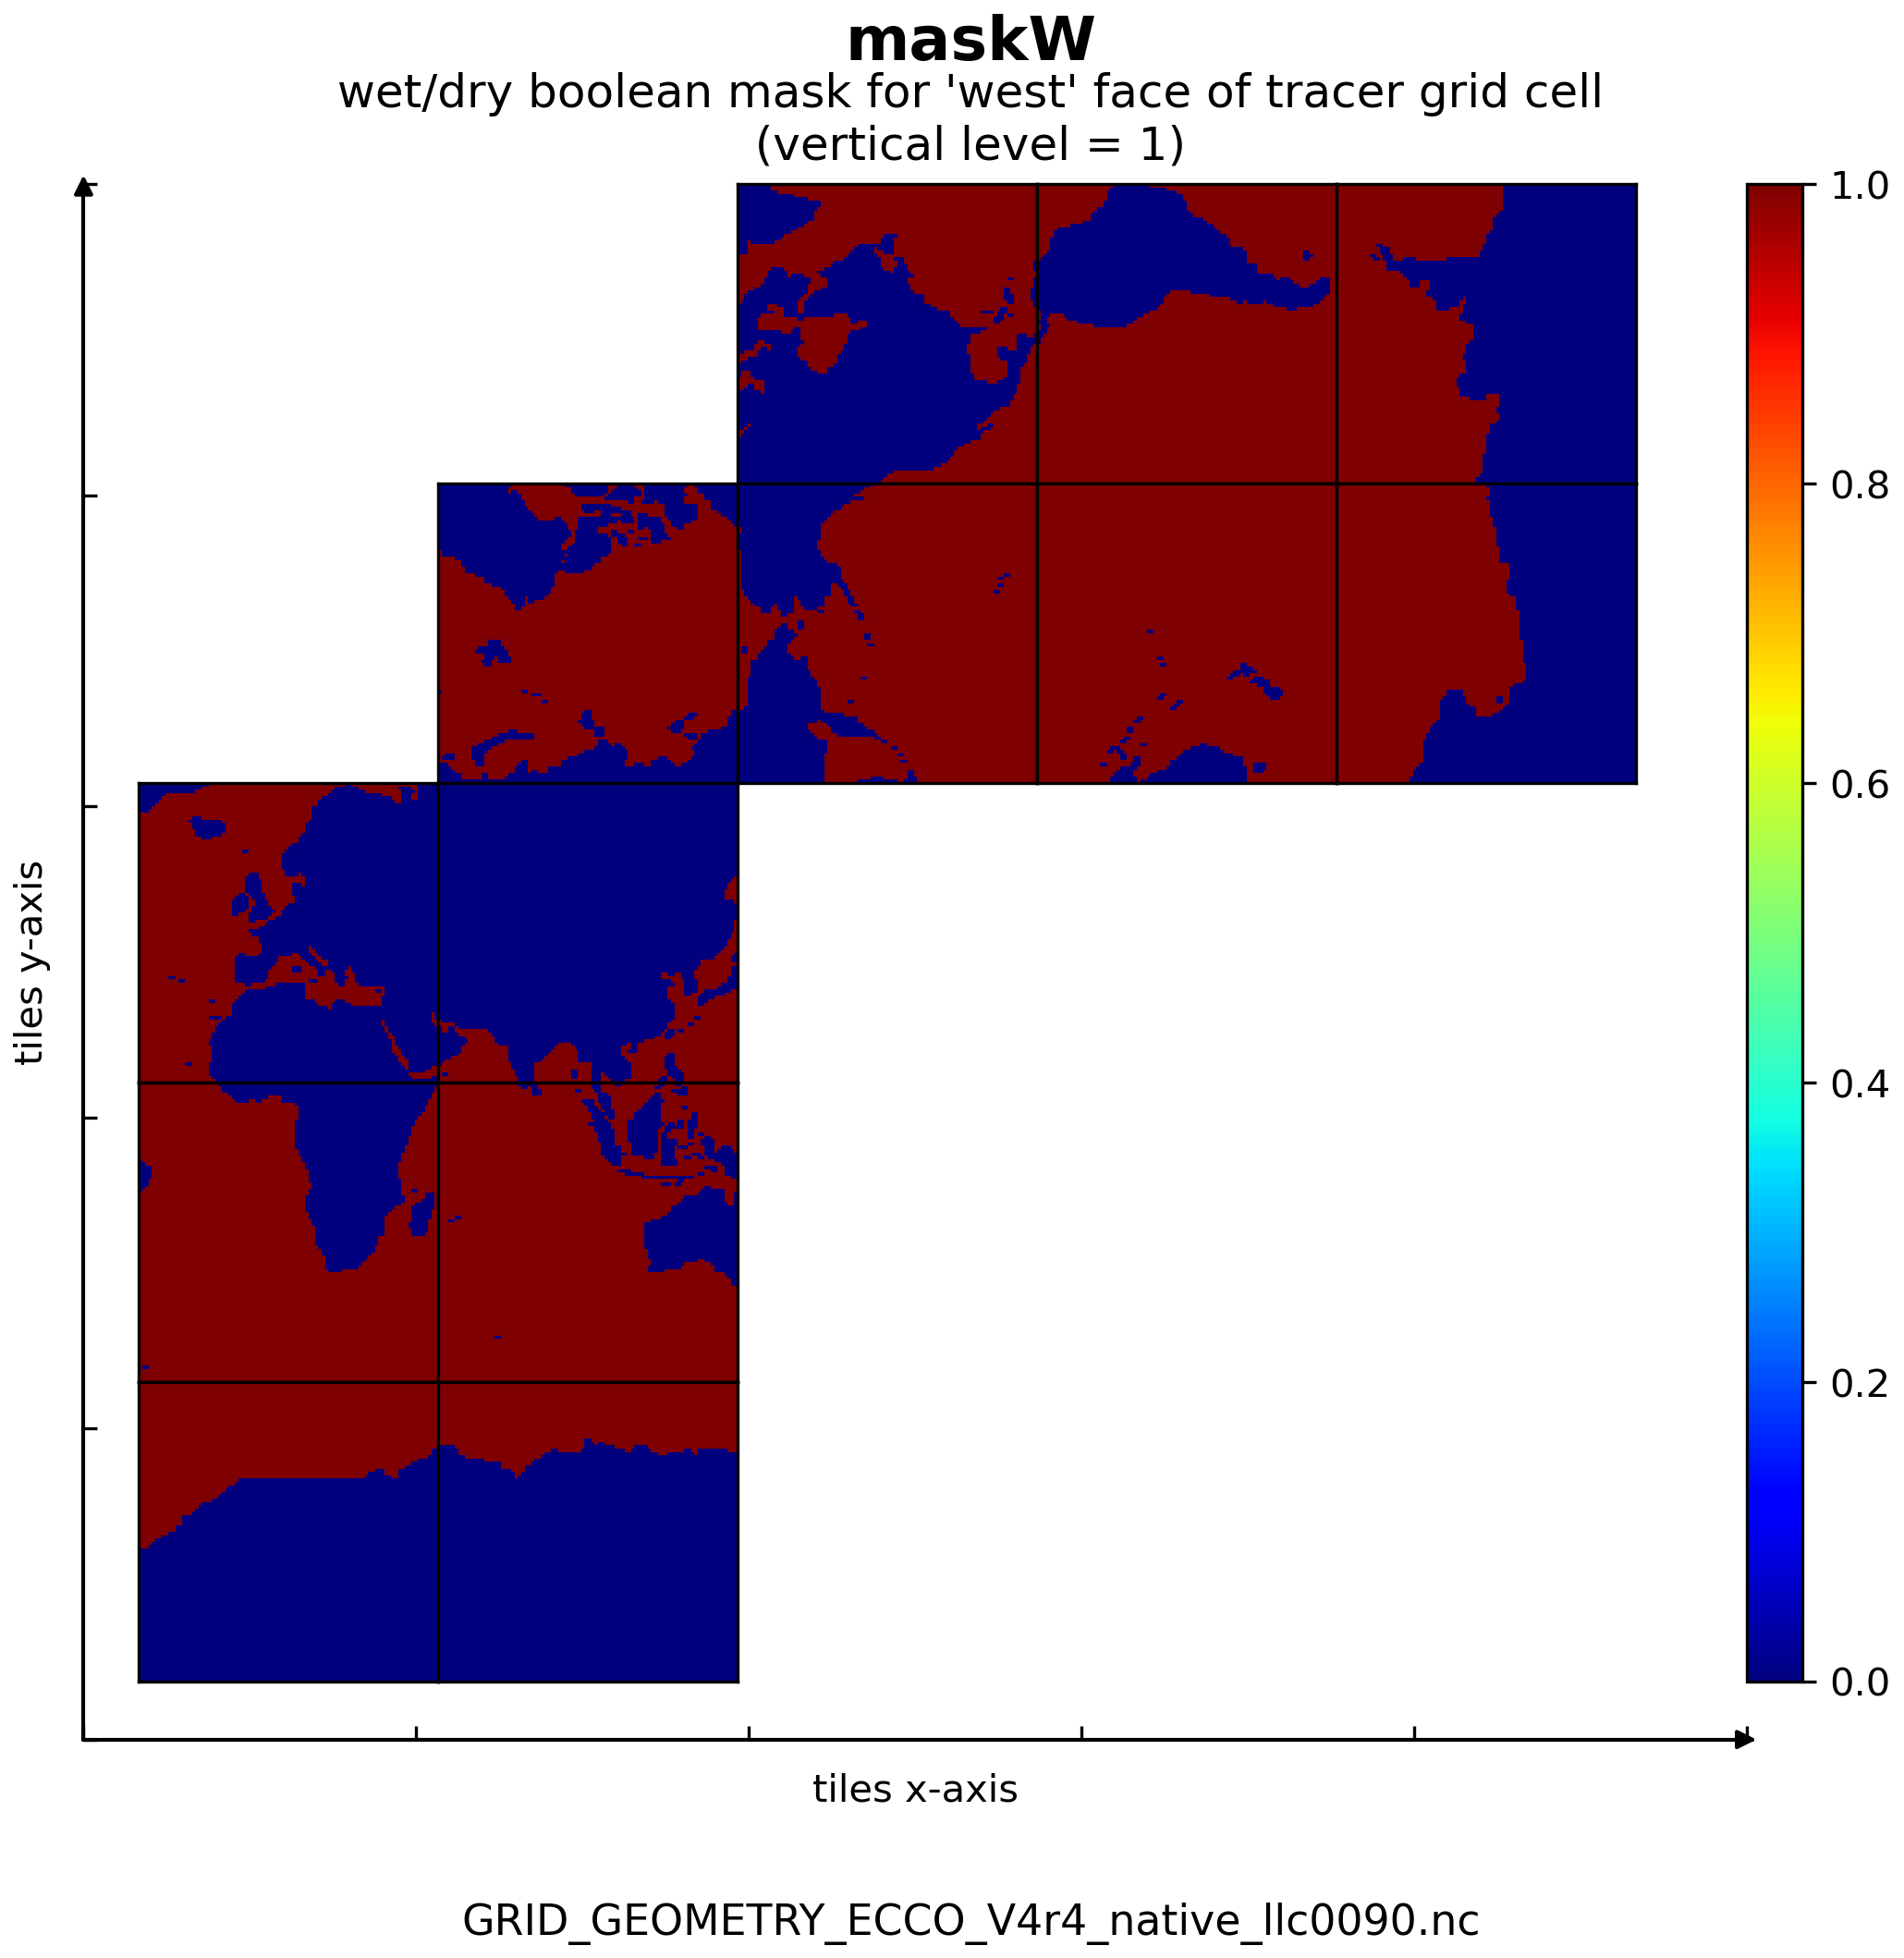
\includegraphics[scale=0.55]{../images/plots/v4r4/native_plots_coords/Geometry_Parameters_for_the_Lat-Lon-Cap_90_(llc90)_Native_Model_Grid_(Version_4_Release_4)/maskW.png}
\caption{Dataset: GRID\_GEOMETRY\_ECCO, Variable: maskW}
\label{tab:table-GRID_GEOMETRY_ECCO_maskW-Plot}
\end{figure}
\newpage
\pagebreak
\subsubsection{Native coordinates Variable: maskS}
\begin{longtable}{|m{0.06\textwidth}|m{0.3\textwidth}|m{0.45\textwidth}|m{0.12\textwidth}|}
\caption{Attributes description of the variable 'maskS' from GRID\_GEOMETRY\_ECCO's  dataset.}
\label{tab:table-GRID_GEOMETRY_ECCO_maskS} \\ 
\hline \endhead \hline \endfoot
\rowcolor{lightgray} \textbf{Storage Type} & \textbf{Variable Name} & \textbf{Description} & \textbf{Unit} \\ \hline
bool & maskS & Wet/dry boolean mask for 'south' face of tracer grid cell & N/A \\ \hline
\multicolumn{4}{|c|}{\cellcolor{lightgray}{\textbf{Description of the variable in Common Data language (CDL)}}} \\ \hline
\multicolumn{4}{|c|}{\fontfamily{lmtt}\selectfont{\makecell{\parbox{.95\textwidth}{\vspace*{0.25cm} \footnotesize{bool maskS(k, tile, j\_g, i)\\
\hspace*{0.5cm}maskS: \_FillValue = 1\\
\hspace*{0.5cm}maskS: coordinates = Z\\
\hspace*{0.5cm}maskS: coverage\_content\_type = modelResult\\
\hspace*{0.5cm}maskS: long\_name = wet/dry boolean mask for south face of tracer grid cell\\
}}}}} \\ \hline
\rowcolor{lightgray} \multicolumn{4}{|c|}{\textbf{Comments}} \\ \hline
\multicolumn{4}{|p{1\textwidth}|}{\footnotesize{{True for grid cells with nonzero open vertical fraction along their 'south' face (hfacs > 0), otherwise false. although hfacs can vary though time, cells will never close if starting open and will never open if starting closed: hfacs(i,j,k,t) > 0 for all t, if hfacs(i,j,k,t=0) and hfacs(i,j,k,t) = 0 for all t, if hfacs(i,j,k,t=0) = 0. therefore, masks is time invariant. note: }}} \\ \hline
\end{longtable}

\begin{figure}[H]
\centering
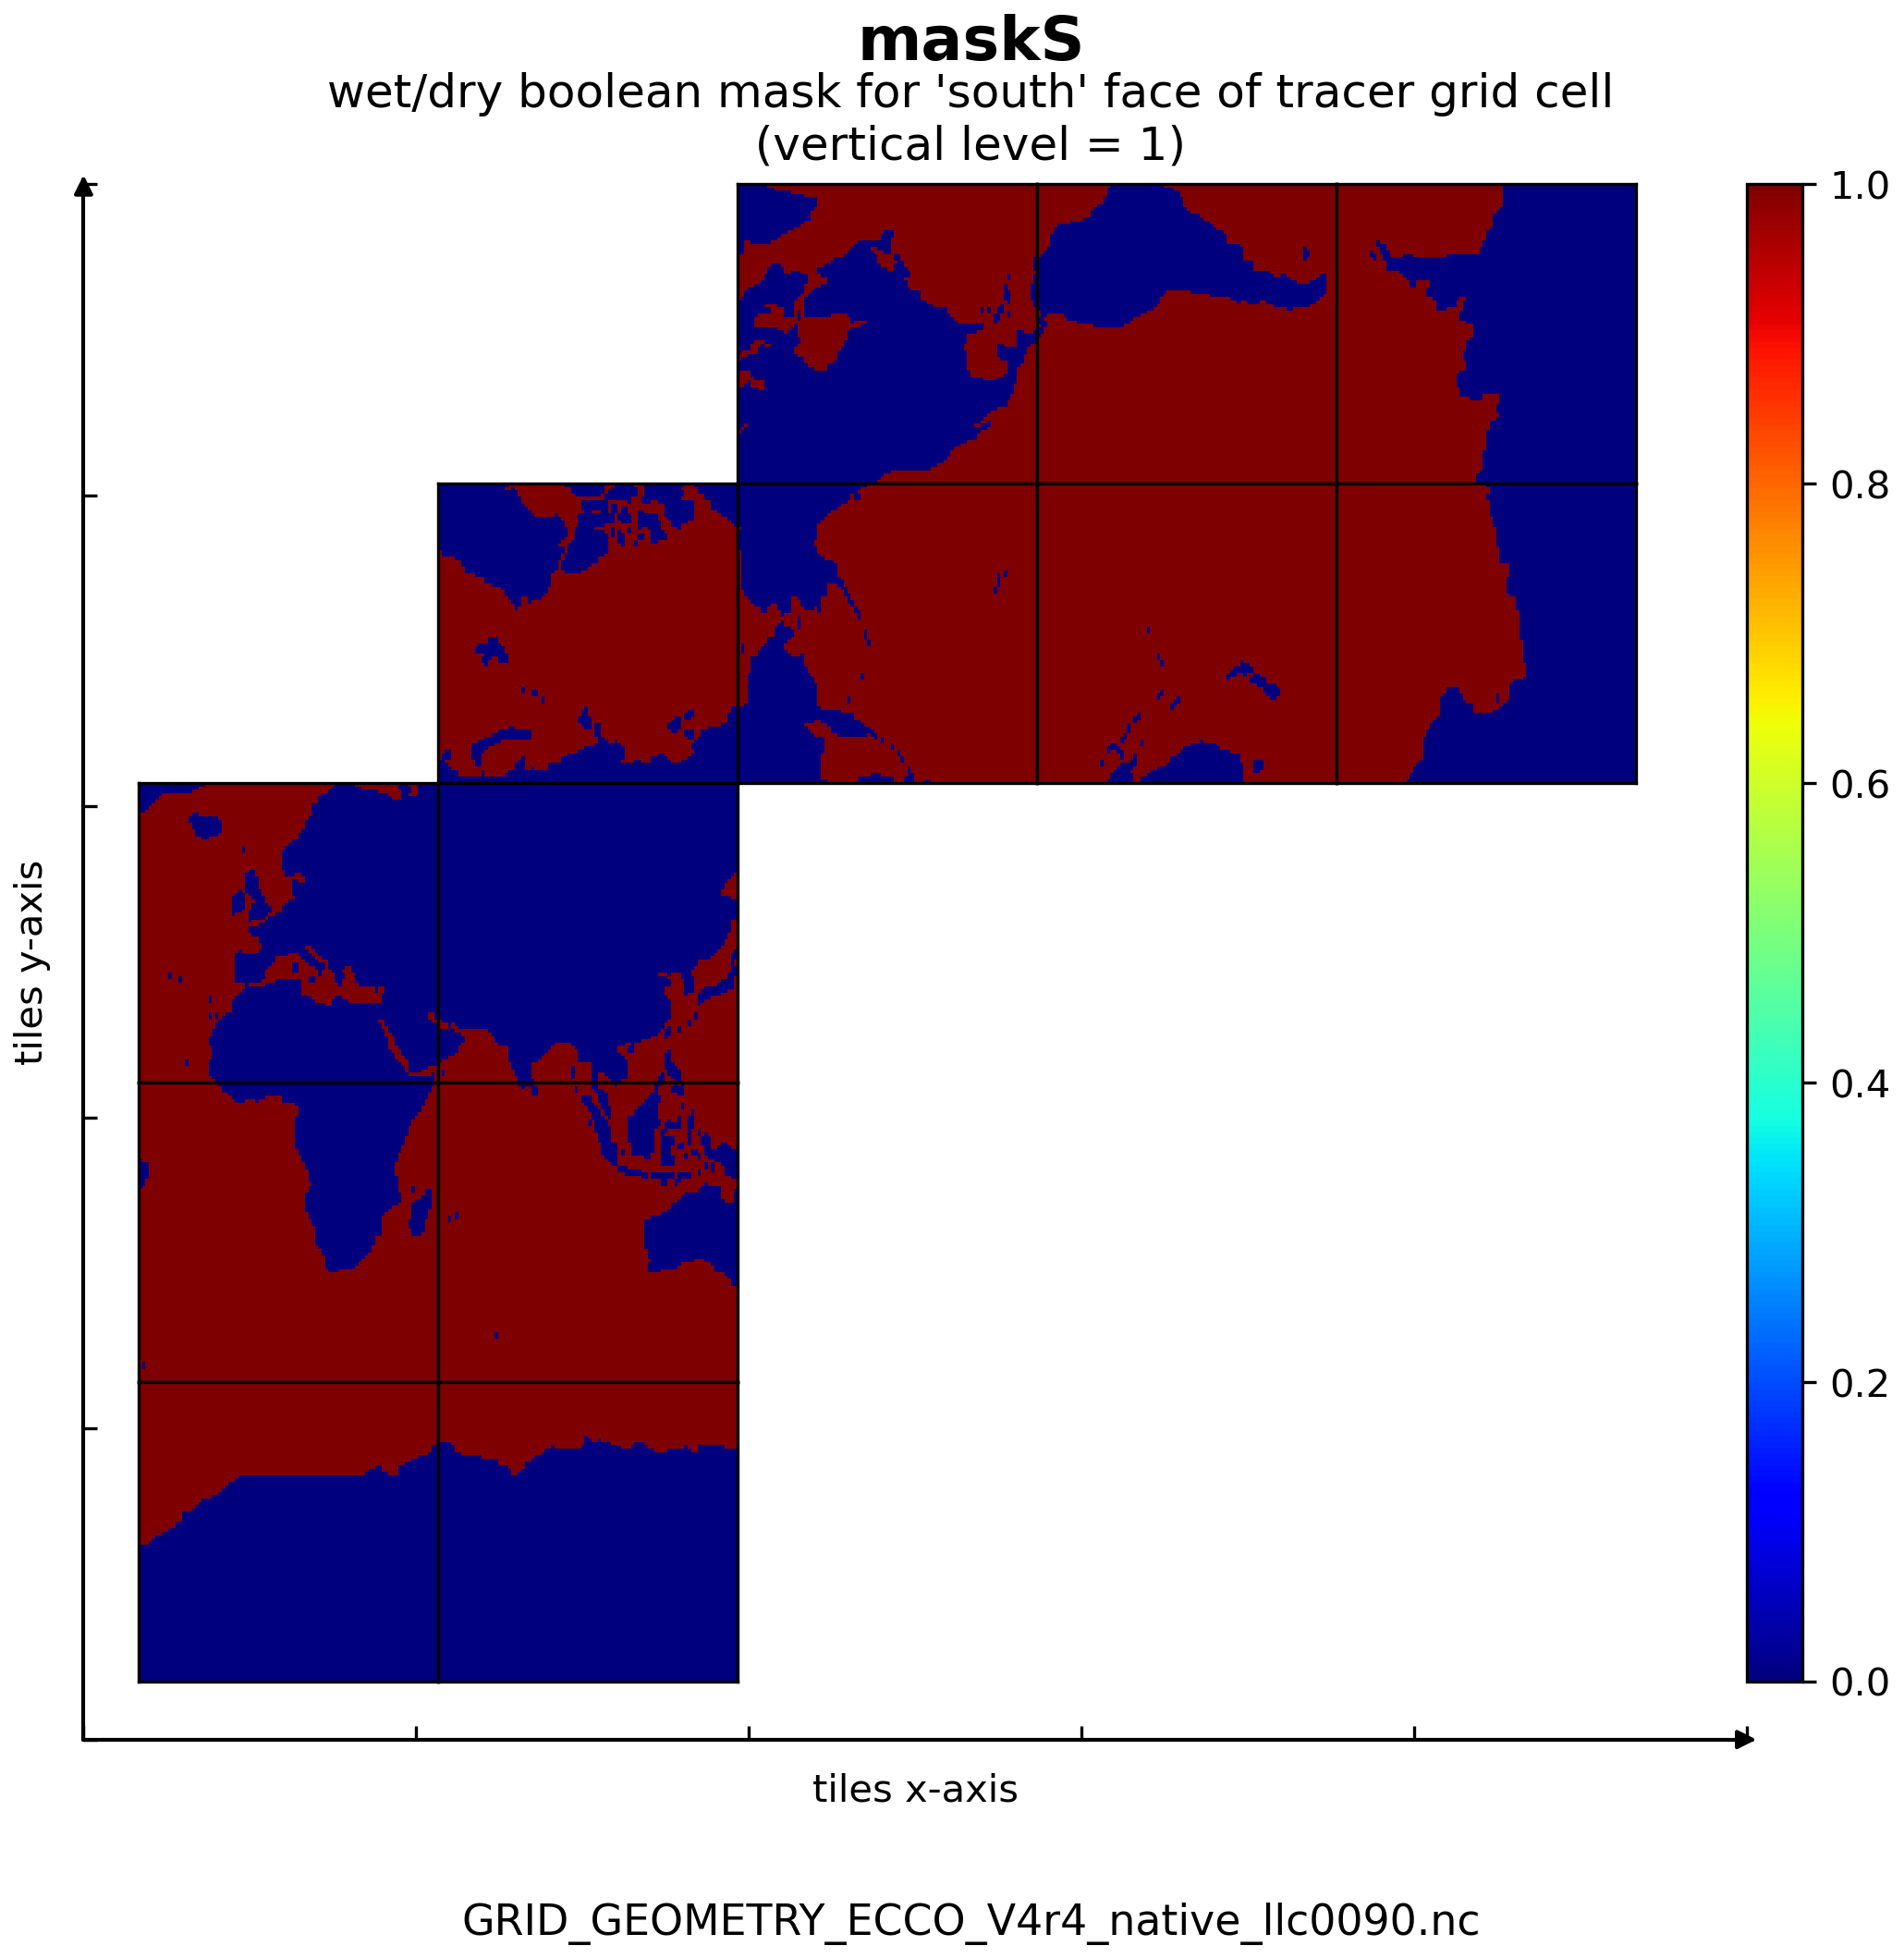
\includegraphics[scale=0.55]{../images/plots/v4r4/native_plots_coords/Geometry_Parameters_for_the_Lat-Lon-Cap_90_(llc90)_Native_Model_Grid_(Version_4_Release_4)/maskS.png}
\caption{Dataset: GRID\_GEOMETRY\_ECCO, Variable: maskS}
\label{tab:table-GRID_GEOMETRY_ECCO_maskS-Plot}
\end{figure}
\newpage
% OK: => static file
\pagebreak
\section{Native Dataset Groupings}
\par\vspace{0.5cm}
\subsection{Overview of the Native Dataset Groupings}
Lorem ipsum dolor sit amet, consectetur adipiscing elit. Vivamus at enim eget nisi ultrices facilisis a et purus. Sed tincidunt scelerisque ligula, in vehicula dui venenatis at. Pellentesque habitant morbi tristique senectus et netus et malesuada fames ac turpis egestas. Curabitur consequat commodo nunc, nec lacinia quam feugiat vel. Integer bibendum lectus sit amet quam elementum, ut pretium quam malesuada. Cras fermentum venenatis augue, id commodo libero facilisis nec. Quisque euismod, odio vitae dapibus convallis, justo enim iaculis metus, vel interdum elit nisi vel lectus. Fusce tempor elit in semper condimentum. Ut quis dui eget purus cursus interdum eu ac elit.'
\par\vspace{0.5cm}

\pagebreak
\subsection{Native NetCDF ATM\_SURFACE\_TEMP\_HUM\_WIND\_PRES}
\newp
\begin{longtable}{|p{0.1\textwidth}|p{0.5\textwidth}|}
\caption{Variables in the dataset ATM\_SURFACE\_TEMP\_HUM\_WIND\_PRES}
\label{tab:table-ATM_SURFACE_TEMP_HUM_WIND_PRES-fields} \\ 
\hline \endhead \hline \endfoot
\rowcolor{lightgray} \textbf{Dataset:} & \textbf{ATM\_SURFACE\_TEMP\_HUM\_WIND\_PRES} \\ \hline
Field: &EXFatemp \\ \hline
Field: &EXFaqh \\ \hline
Field: &EXFuwind \\ \hline
Field: &EXFvwind \\ \hline
Field: &EXFwspee \\ \hline
Field: &EXFpress \\ \hline
\end{longtable}

\pagebreak
\subsubsection{Native Variable EXFaqh}
\begin{longtable}{|p{0.06\textwidth}|p{0.41\textwidth}|p{0.39\textwidth}|p{0.06\textwidth}|}
\caption{CDL description of ATM\_SURFACE\_TEMP\_HUM\_WIND\_PRES's EXFaqh variable}
\label{tab:table-ATM_SURFACE_TEMP_HUM_WIND_PRES_EXFaqh} \\ 
\hline \endhead \hline \endfoot
\rowcolor{lightgray} \textbf{Storage Type} & \textbf{Variable Name} & \textbf{Description} & \textbf{Unit} \\ \hline
float32 & EXFaqh & Atmosphere surface (2 m) specific humidity  & kg kg-1 \\ \hline
\rowcolor{lightgray}  \multicolumn{4}{|p{1.00\textwidth}|}{\textbf{CDL Description}} \\ \hline
\multicolumn{4}{|p{1.00\textwidth}|}{\makecell{\parbox{1\textwidth}{float32 EXFaqh(time, tile, j, i)\\
\hspace*{0.5cm}EXFaqh: \_FillValue = 9.96921e+36\\
\hspace*{0.5cm}EXFaqh: long\_name = Atmosphere surface (2 m) specific humidity \\
\hspace*{0.5cm}EXFaqh: units = kg kg: 1\\
\hspace*{0.5cm}EXFaqh: coverage\_content\_type = modelResult\\
\hspace*{0.5cm}EXFaqh: standard\_name = surface\_specific\_humidity\\
\hspace*{0.5cm}EXFaqh: coordinates = time XC YC\\
\hspace*{0.5cm}EXFaqh: valid\_min = : 0.0014020215021446347\\
\hspace*{0.5cm}EXFaqh: valid\_max = 0.03014513850212097}}} \\ \hline
\rowcolor{lightgray} \multicolumn{4}{|p{1.00\textwidth}|}{\textbf{Comments}} \\ \hline
\multicolumn{4}{|p{1\textwidth}|}{Surface (2 m) specific humidity over open water. Note: sum of ERA-Interim surface specific humidity and the control adjustment from ocean state estimation.} \\ \hline
\end{longtable}

\begin{figure}[H]
\centering
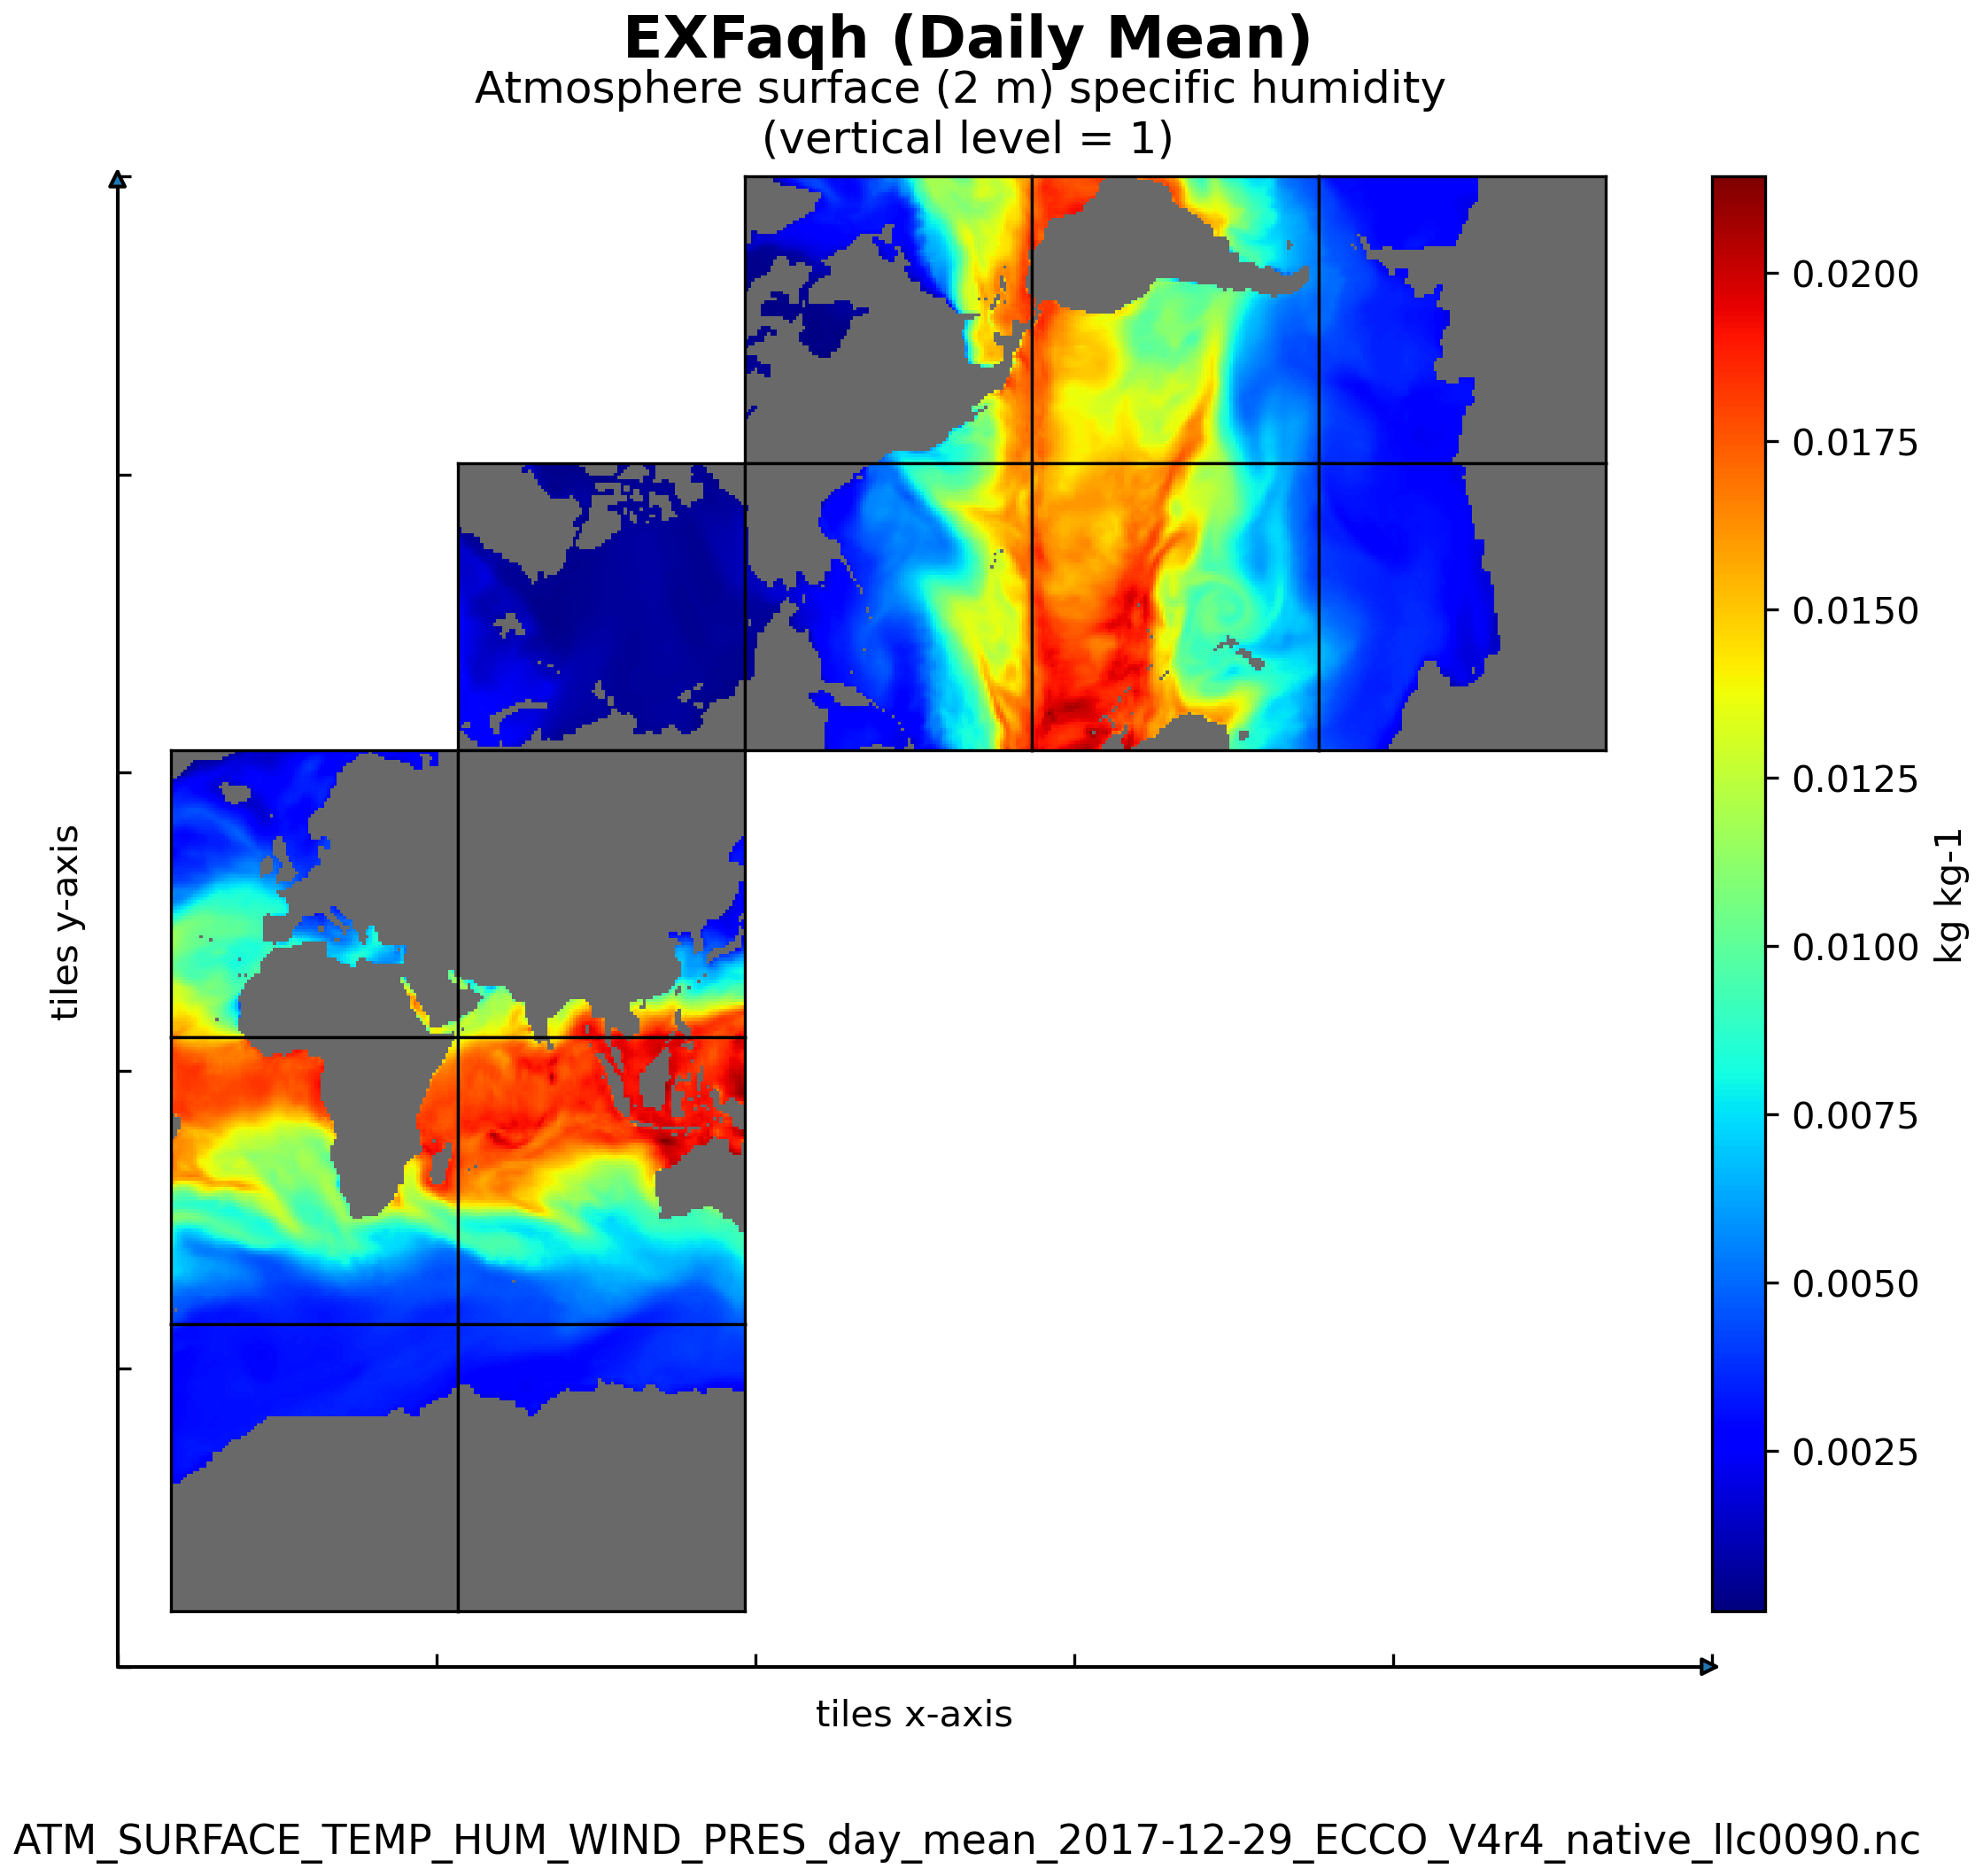
\includegraphics[scale=0.5]{../images/plots/native_plots/Atmosphere_Surface_Temperature_Humidity_Wind_and_Pressure/EXFaqh.png}
\caption{\\Dataset: ATM\_SURFACE\_TEMP\_HUM\_WIND\_PRES\\Variable: EXFaqh}
\label{tab:table-ATM_SURFACE_TEMP_HUM_WIND_PRES_EXFaqh-Plot}
\end{figure}
\pagebreak
\subsubsection{Native Variable EXFatemp}
\begin{longtable}{|p{0.06\textwidth}|p{0.41\textwidth}|p{0.39\textwidth}|p{0.06\textwidth}|}
\caption{CDL description of ATM\_SURFACE\_TEMP\_HUM\_WIND\_PRES's EXFatemp variable}
\label{tab:table-ATM_SURFACE_TEMP_HUM_WIND_PRES_EXFatemp} \\ 
\hline \endhead \hline \endfoot
\rowcolor{lightgray} \textbf{Storage Type} & \textbf{Variable Name} & \textbf{Description} & \textbf{Unit} \\ \hline
float32 & EXFatemp & Atmosphere surface (2 m) air temperature  & degree\_K \\ \hline
\rowcolor{lightgray}  \multicolumn{4}{|p{1.00\textwidth}|}{\textbf{CDL Description}} \\ \hline
\multicolumn{4}{|p{1.00\textwidth}|}{\makecell{\parbox{1\textwidth}{float32 EXFatemp(time, tile, j, i)\\
\hspace*{0.5cm}EXFatemp: \_FillValue = 9.96921e+36\\
\hspace*{0.5cm}EXFatemp: long\_name = Atmosphere surface (2 m) air temperature \\
\hspace*{0.5cm}EXFatemp: units = degree\_K\\
\hspace*{0.5cm}EXFatemp: coverage\_content\_type = modelResult\\
\hspace*{0.5cm}EXFatemp: standard\_name = air\_temperature\\
\hspace*{0.5cm}EXFatemp: coordinates = time XC YC\\
\hspace*{0.5cm}EXFatemp: valid\_min = 195.37054443359375\\
\hspace*{0.5cm}EXFatemp: valid\_max = 312.8451232910156}}} \\ \hline
\rowcolor{lightgray} \multicolumn{4}{|p{1.00\textwidth}|}{\textbf{Comments}} \\ \hline
\multicolumn{4}{|p{1\textwidth}|}{Surface (2 m) air temperature over open water. Note: sum of ERA-Interim surface air temperature and the control adjustment from ocean state estimation.} \\ \hline
\end{longtable}

\begin{figure}[H]
\centering
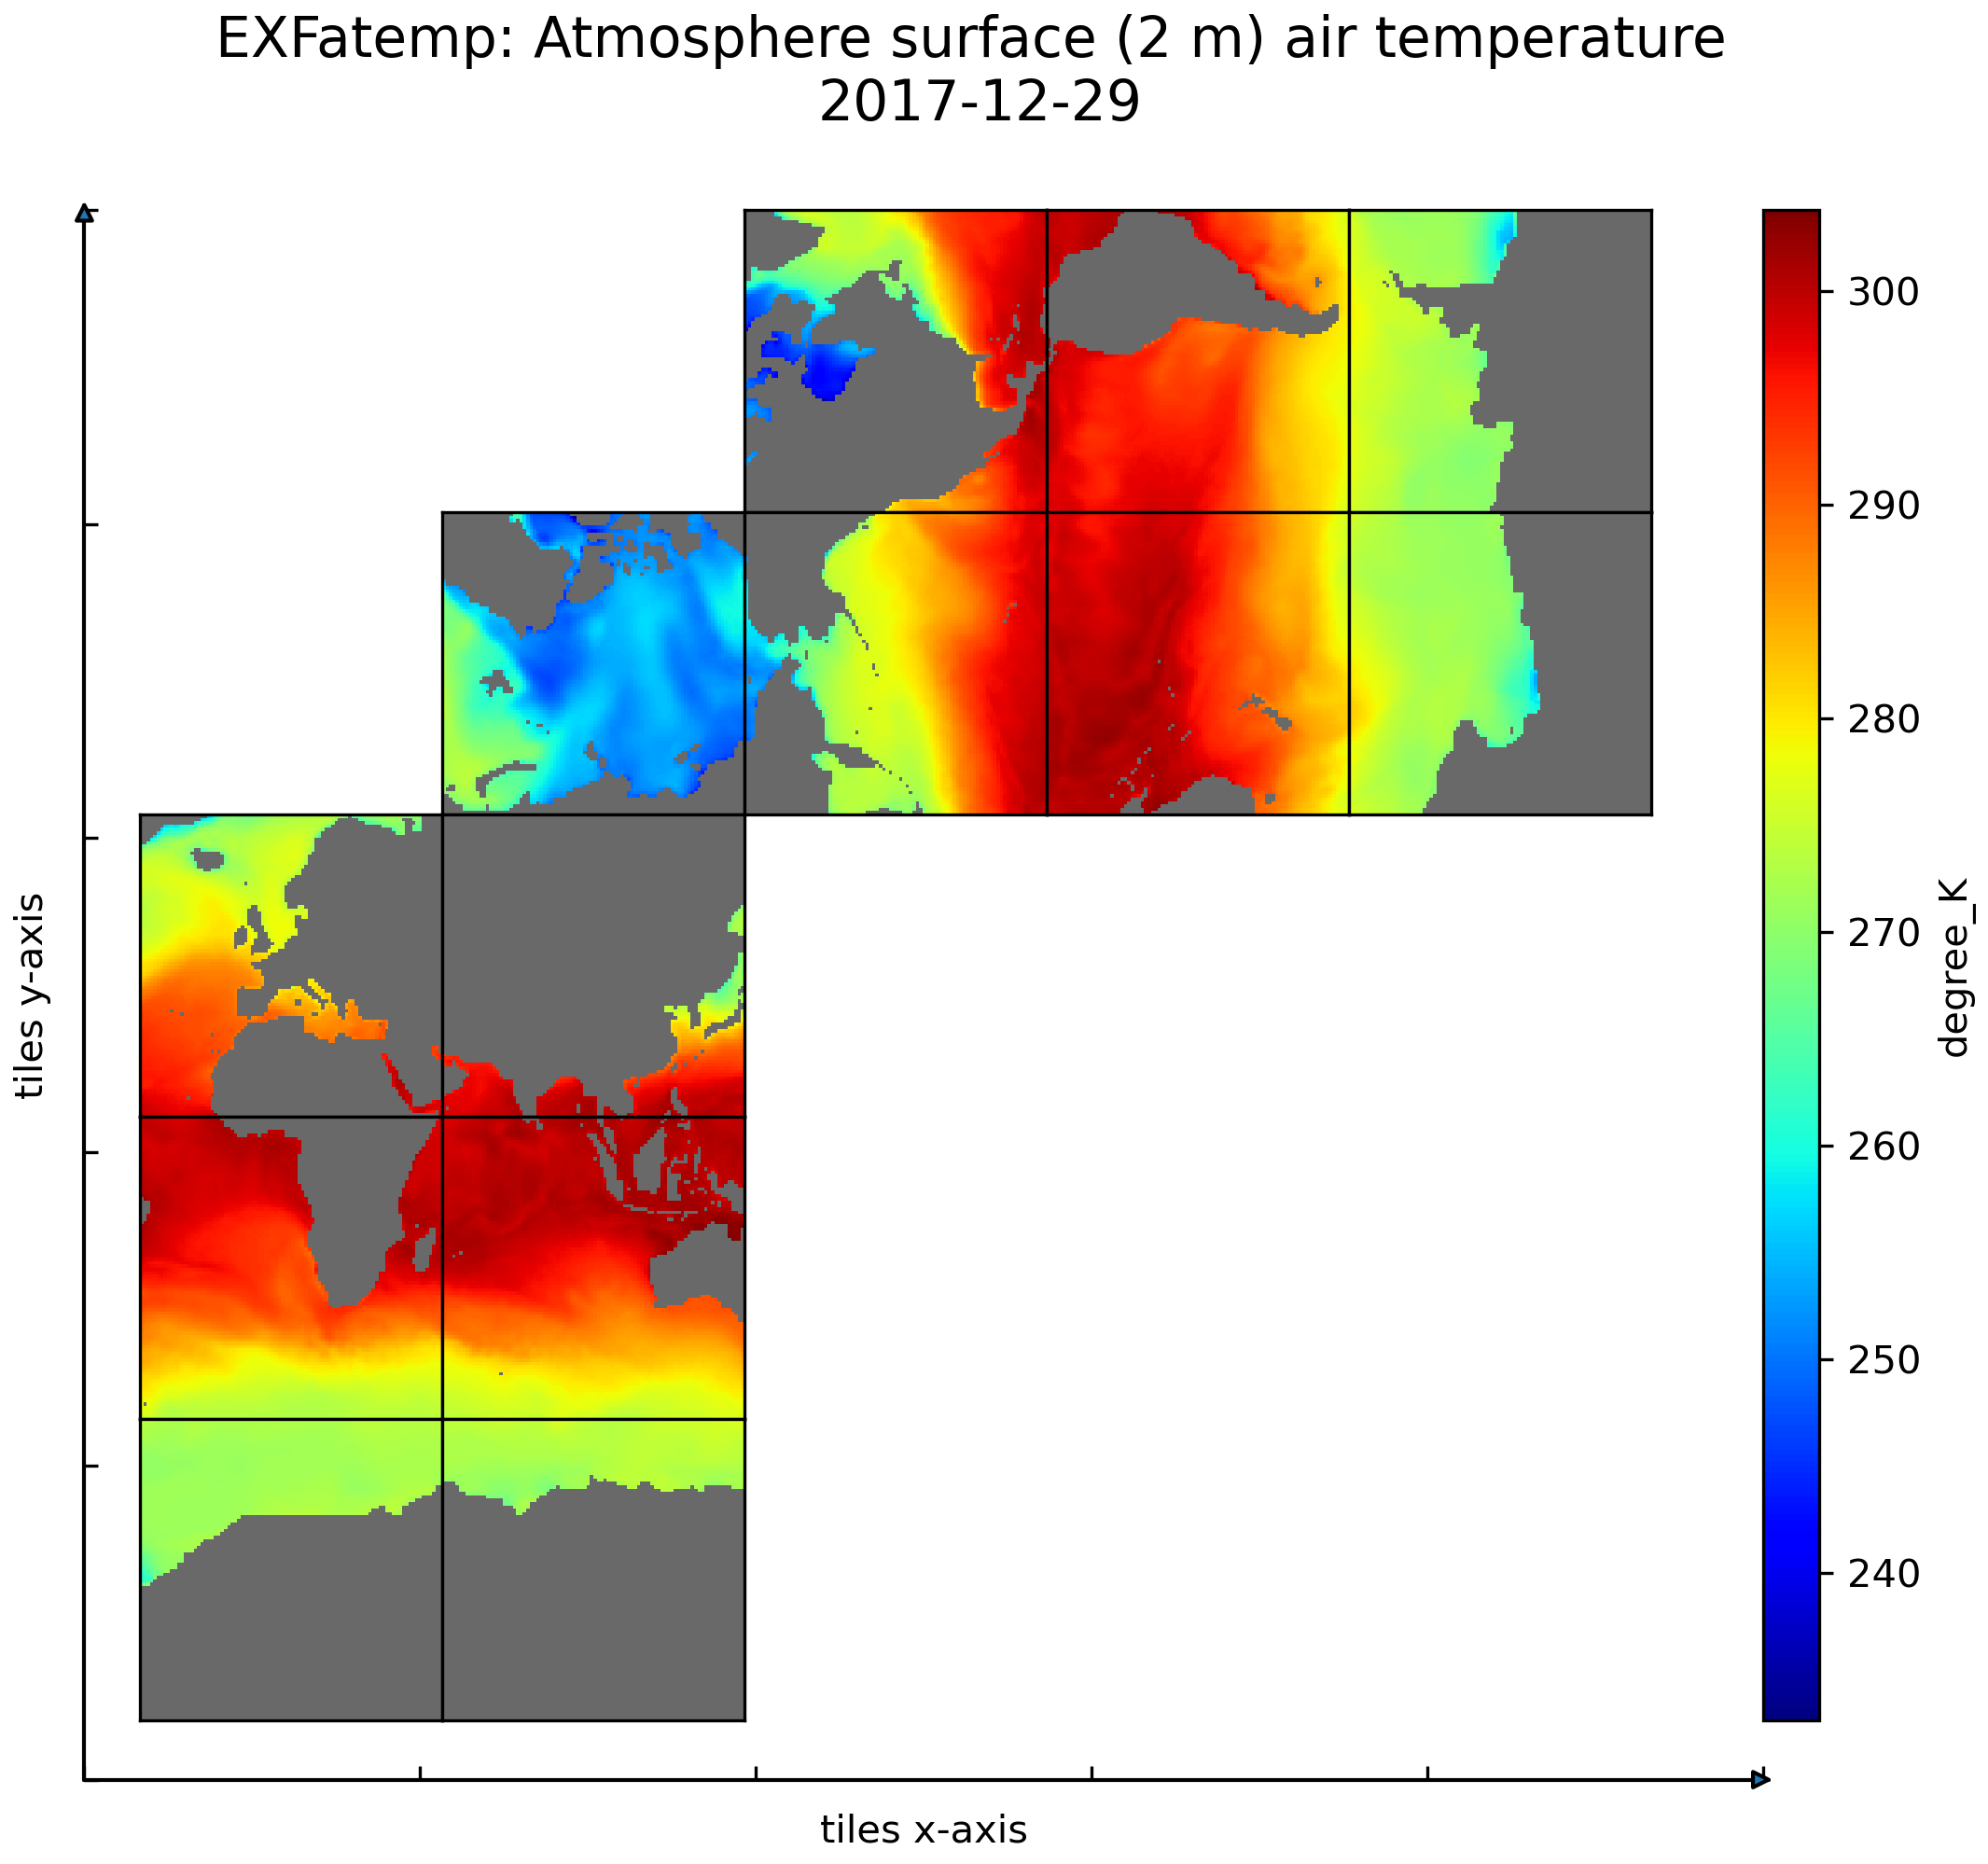
\includegraphics[scale=0.5]{../images/plots/native_plots/Atmosphere_Surface_Temperature_Humidity_Wind_and_Pressure/EXFatemp.png}
\caption{\\Dataset: ATM\_SURFACE\_TEMP\_HUM\_WIND\_PRES\\Variable: EXFatemp}
\label{tab:table-ATM_SURFACE_TEMP_HUM_WIND_PRES_EXFatemp-Plot}
\end{figure}
\pagebreak
\subsubsection{Native Variable EXFpress}
\begin{longtable}{|p{0.06\textwidth}|p{0.41\textwidth}|p{0.39\textwidth}|p{0.06\textwidth}|}
\caption{CDL description of ATM\_SURFACE\_TEMP\_HUM\_WIND\_PRES's EXFpress variable}
\label{tab:table-ATM_SURFACE_TEMP_HUM_WIND_PRES_EXFpress} \\ 
\hline \endhead \hline \endfoot
\rowcolor{lightgray} \textbf{Storage Type} & \textbf{Variable Name} & \textbf{Description} & \textbf{Unit} \\ \hline
float32 & EXFpress & Atmosphere surface pressure & N m-2 \\ \hline
\rowcolor{lightgray}  \multicolumn{4}{|p{1.00\textwidth}|}{\textbf{CDL Description}} \\ \hline
\multicolumn{4}{|p{1.00\textwidth}|}{\makecell{\parbox{1\textwidth}{float32 EXFpress(time, tile, j, i)\\
\hspace*{0.5cm}EXFpress: \_FillValue = 9.96921e+36\\
\hspace*{0.5cm}EXFpress: long\_name = Atmosphere surface pressure\\
\hspace*{0.5cm}EXFpress: units = N m: 2\\
\hspace*{0.5cm}EXFpress: coverage\_content\_type = modelResult\\
\hspace*{0.5cm}EXFpress: standard\_name = surface\_air\_pressure\\
\hspace*{0.5cm}EXFpress: coordinates = time XC YC\\
\hspace*{0.5cm}EXFpress: valid\_min = 92044.171875\\
\hspace*{0.5cm}EXFpress: valid\_max = 106314.7734375}}} \\ \hline
\rowcolor{lightgray} \multicolumn{4}{|p{1.00\textwidth}|}{\textbf{Comments}} \\ \hline
\multicolumn{4}{|p{1\textwidth}|}{Atmospheric pressure field at sea level. Note: ERA-Interim atmospheric pressure, with air tides removed using a variety of methods. Not adjusted by the ocean state estimation.} \\ \hline
\end{longtable}

\begin{figure}[H]
\centering
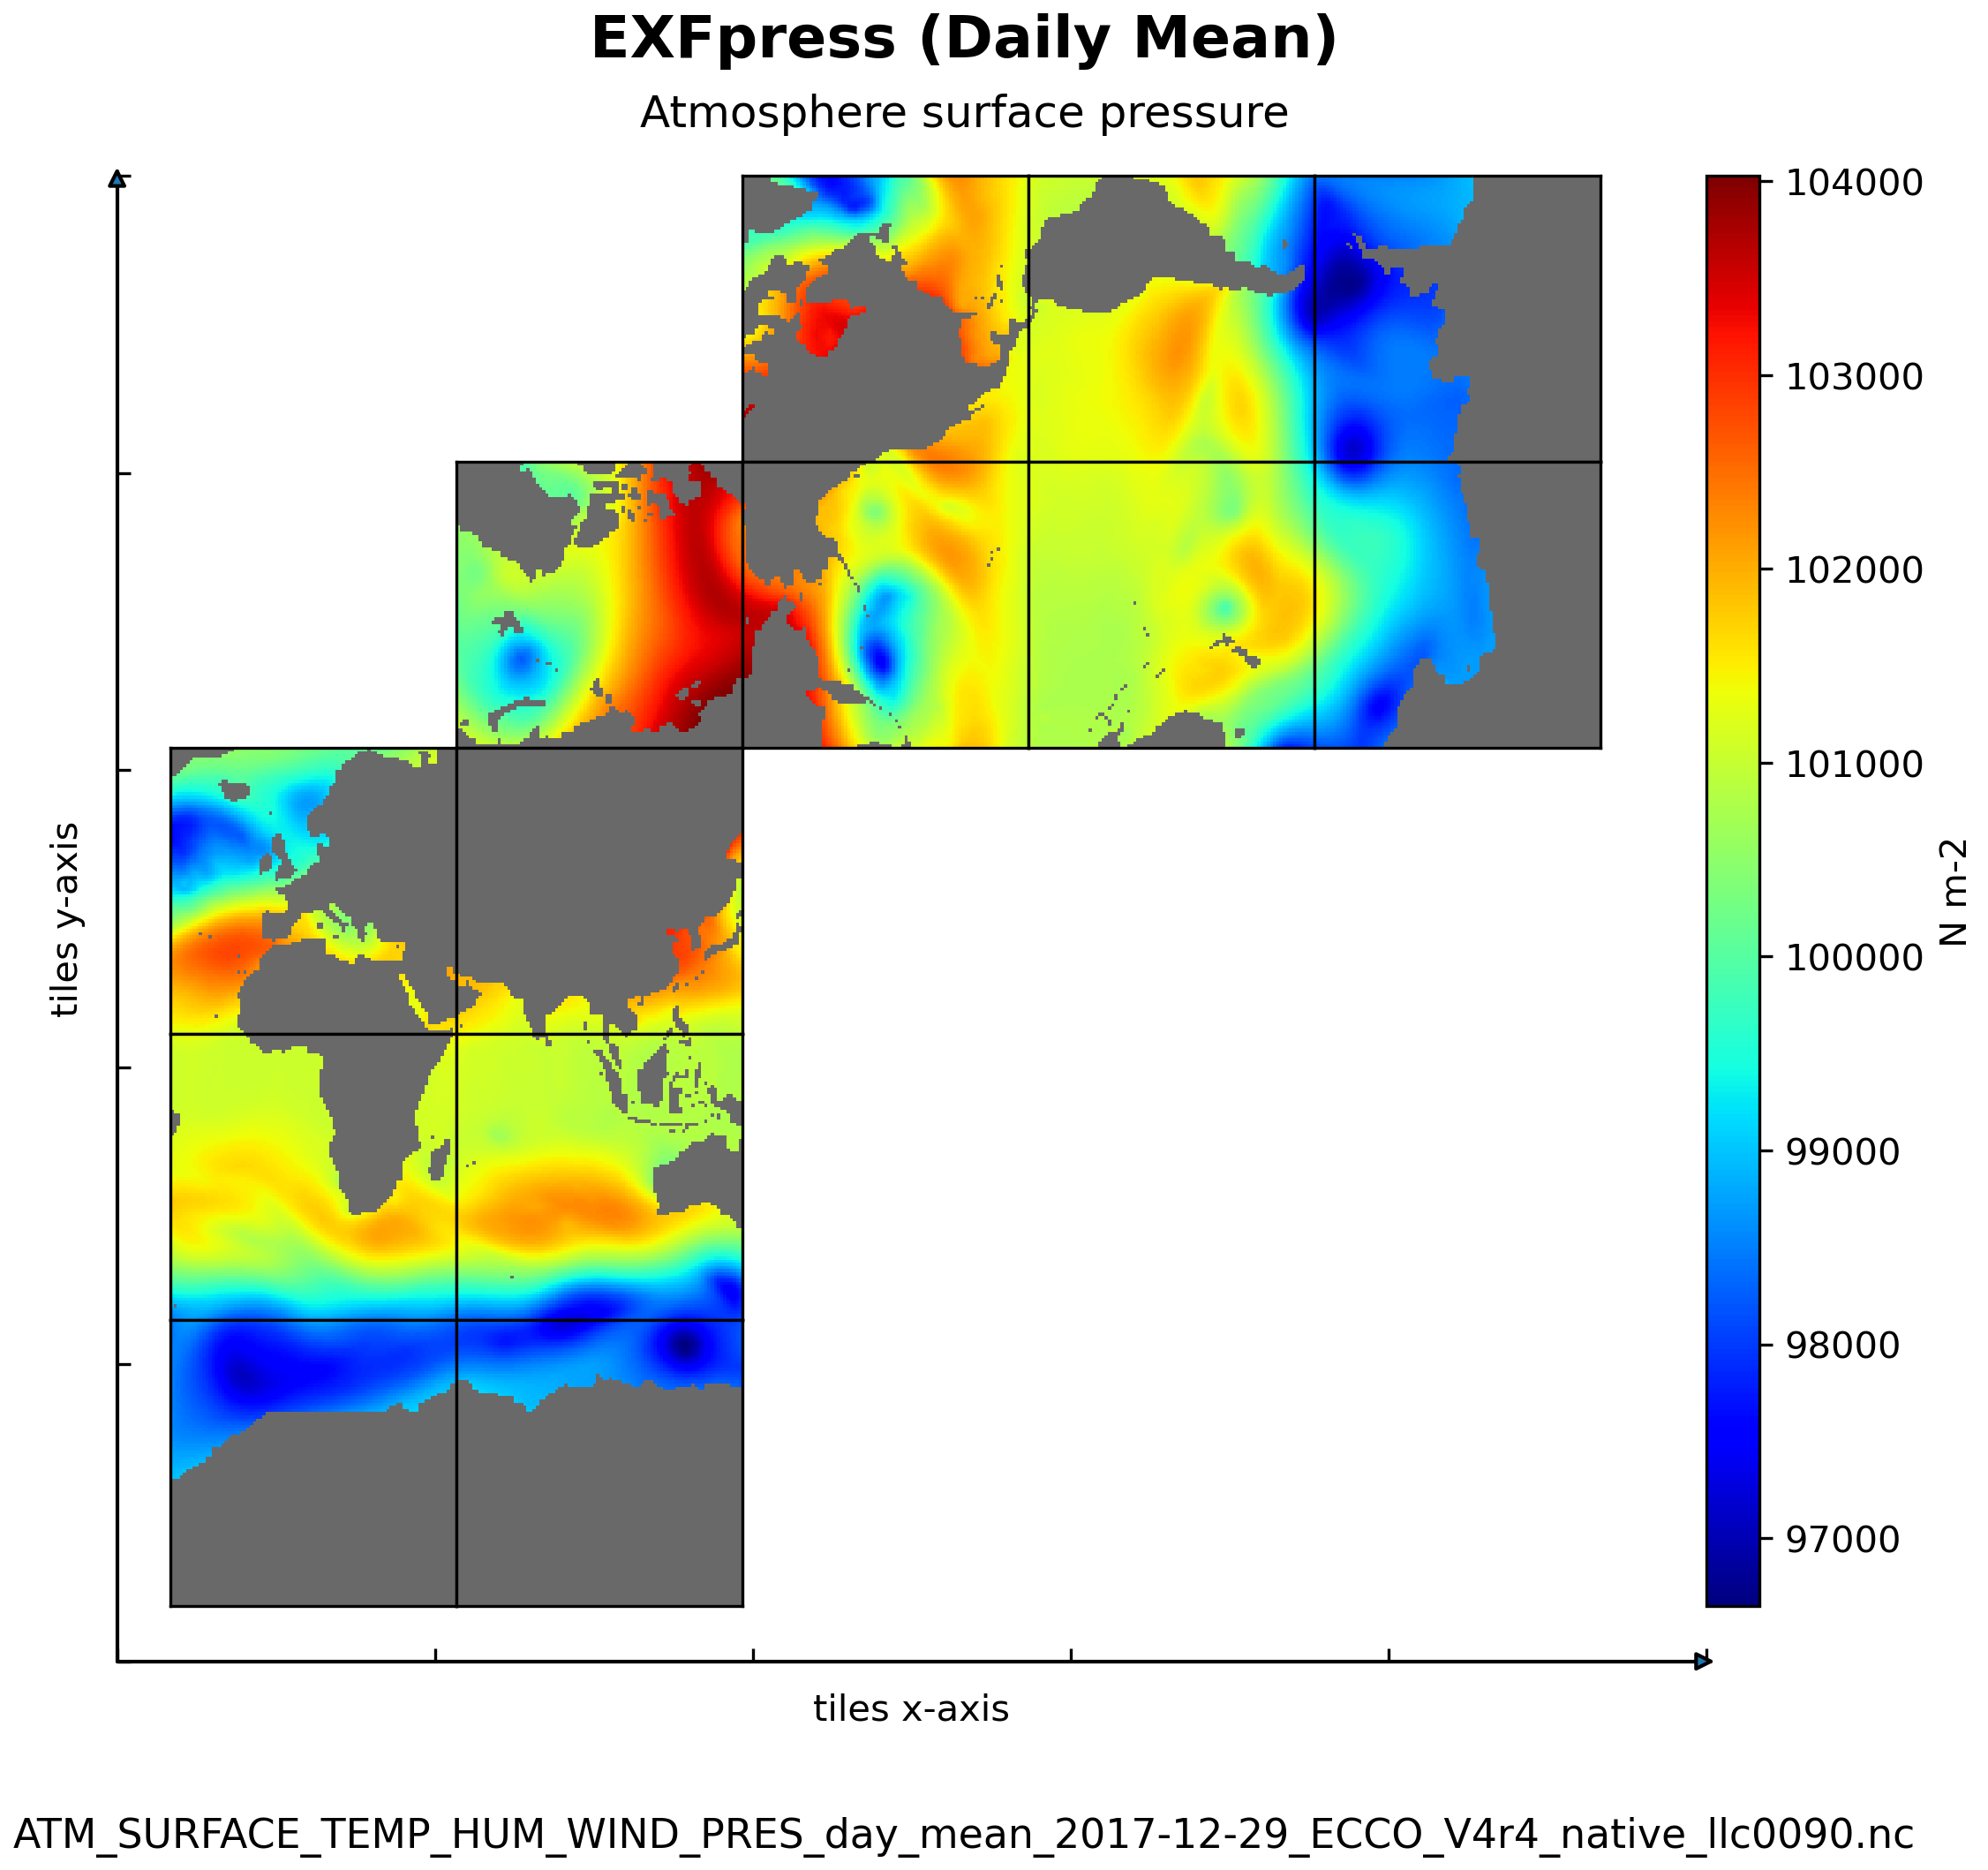
\includegraphics[scale=0.5]{../images/plots/native_plots/Atmosphere_Surface_Temperature_Humidity_Wind_and_Pressure/EXFpress.png}
\caption{\\Dataset: ATM\_SURFACE\_TEMP\_HUM\_WIND\_PRES\\Variable: EXFpress}
\label{tab:table-ATM_SURFACE_TEMP_HUM_WIND_PRES_EXFpress-Plot}
\end{figure}
\pagebreak
\subsubsection{Native Variable EXFuwind}
\begin{longtable}{|p{0.06\textwidth}|p{0.41\textwidth}|p{0.39\textwidth}|p{0.06\textwidth}|}
\caption{CDL description of ATM\_SURFACE\_TEMP\_HUM\_WIND\_PRES's EXFuwind variable}
\label{tab:table-ATM_SURFACE_TEMP_HUM_WIND_PRES_EXFuwind} \\ 
\hline \endhead \hline \endfoot
\rowcolor{lightgray} \textbf{Storage Type} & \textbf{Variable Name} & \textbf{Description} & \textbf{Unit} \\ \hline
float32 & EXFuwind & Wind speed at 10m in the model +x direction & m s-1 \\ \hline
\rowcolor{lightgray}  \multicolumn{4}{|p{1.00\textwidth}|}{\textbf{CDL Description}} \\ \hline
\multicolumn{4}{|p{1.00\textwidth}|}{\makecell{\parbox{1\textwidth}{float32 EXFuwind(time, tile, j, i)\\
\hspace*{0.5cm}EXFuwind: \_FillValue = 9.96921e+36\\
\hspace*{0.5cm}EXFuwind: long\_name = Wind speed at 10m in the model +x direction\\
\hspace*{0.5cm}EXFuwind: units = m s: 1\\
\hspace*{0.5cm}EXFuwind: coverage\_content\_type = modelResult\\
\hspace*{0.5cm}EXFuwind: standard\_name = x\_wind\\
\hspace*{0.5cm}EXFuwind: coordinates = time XC YC\\
\hspace*{0.5cm}EXFuwind: valid\_min = : 34.528900146484375\\
\hspace*{0.5cm}EXFuwind: valid\_max = 29.92486572265625}}} \\ \hline
\rowcolor{lightgray} \multicolumn{4}{|p{1.00\textwidth}|}{\textbf{Comments}} \\ \hline
\multicolumn{4}{|p{1\textwidth}|}{Wind speed at 10m in the +x direction at the tracer cell on the native model grid. Note: ECCO v4r4 is forced with wind stress (see EXFtaux) not vector winds converted to wind stress using bulk formulae. EXFuwind is calculated by converting wind stress to vector wind using bulk formulae.} \\ \hline
\end{longtable}

\begin{figure}[H]
\centering
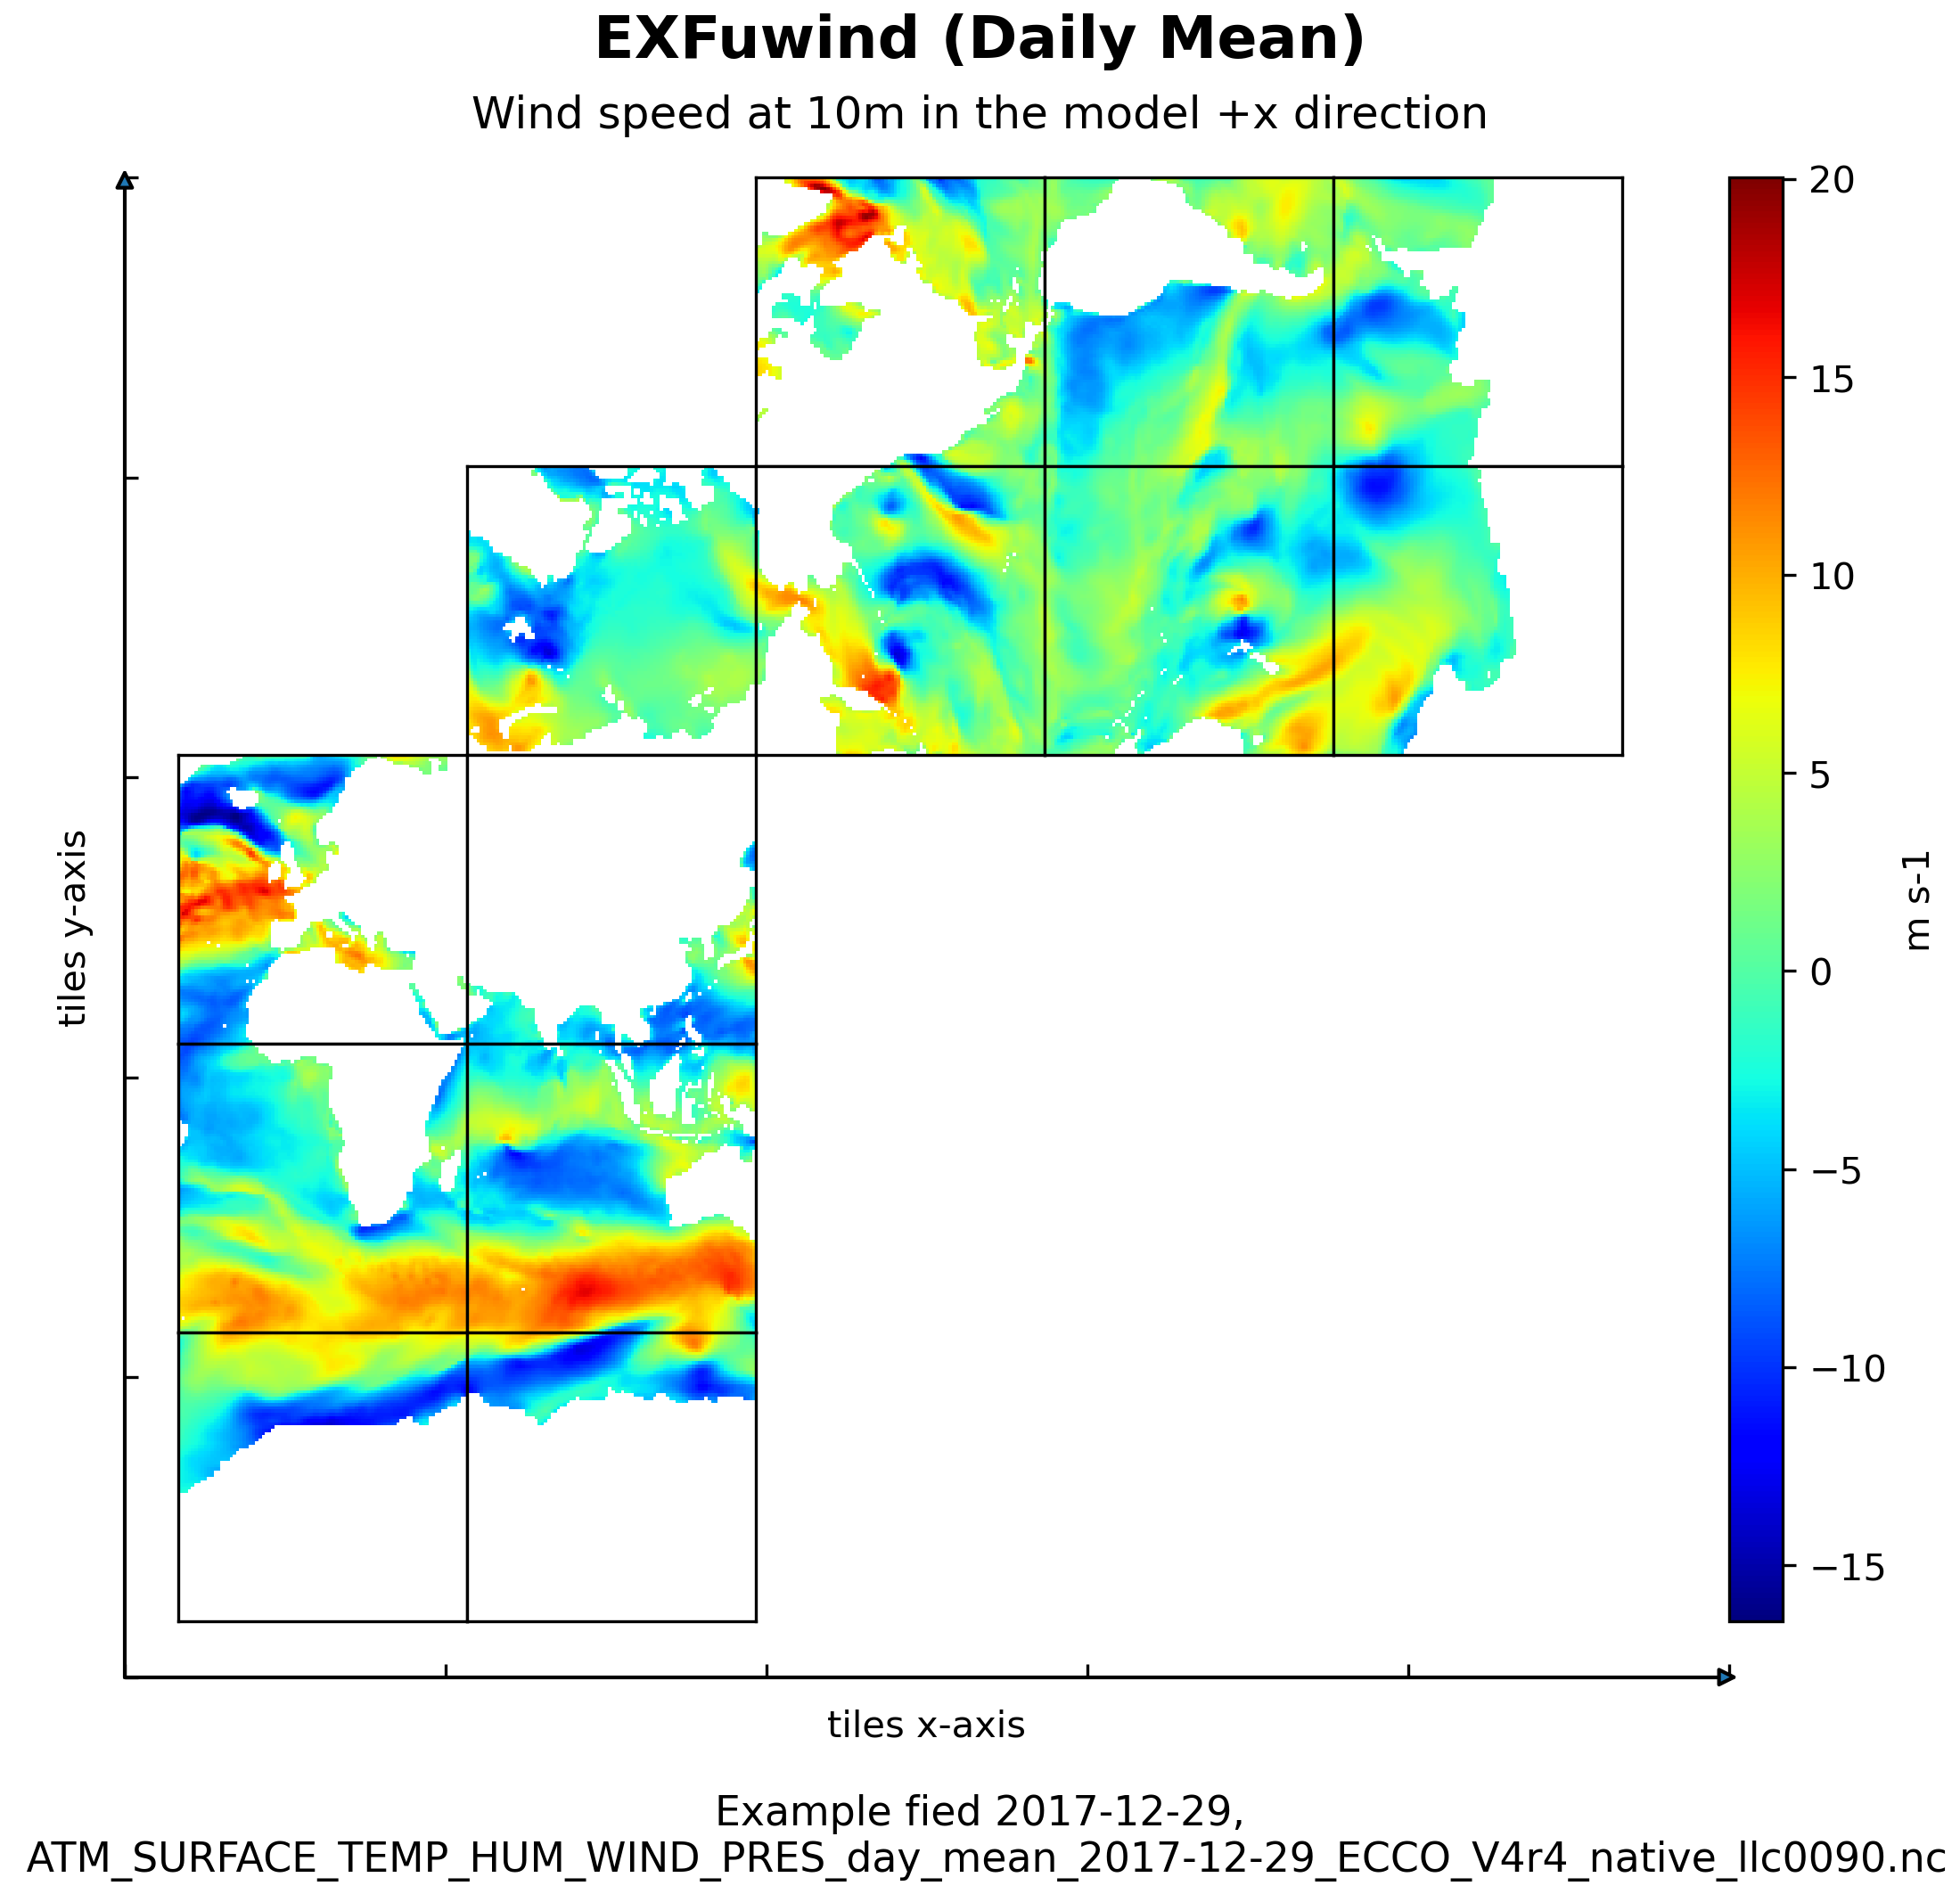
\includegraphics[scale=0.5]{../images/plots/native_plots/Atmosphere_Surface_Temperature_Humidity_Wind_and_Pressure/EXFuwind.png}
\caption{\\Dataset: ATM\_SURFACE\_TEMP\_HUM\_WIND\_PRES\\Variable: EXFuwind}
\label{tab:table-ATM_SURFACE_TEMP_HUM_WIND_PRES_EXFuwind-Plot}
\end{figure}
\pagebreak
\subsubsection{Native Variable EXFvwind}
\begin{longtable}{|p{0.06\textwidth}|p{0.41\textwidth}|p{0.39\textwidth}|p{0.06\textwidth}|}
\caption{CDL description of ATM\_SURFACE\_TEMP\_HUM\_WIND\_PRES's EXFvwind variable}
\label{tab:table-ATM_SURFACE_TEMP_HUM_WIND_PRES_EXFvwind} \\ 
\hline \endhead \hline \endfoot
\rowcolor{lightgray} \textbf{Storage Type} & \textbf{Variable Name} & \textbf{Description} & \textbf{Unit} \\ \hline
float32 & EXFvwind & Wind speed at 10m in the model +y direction & m s-1 \\ \hline
\rowcolor{lightgray}  \multicolumn{4}{|p{1.00\textwidth}|}{\textbf{CDL Description}} \\ \hline
\multicolumn{4}{|p{1.00\textwidth}|}{\makecell{\parbox{1\textwidth}{float32 EXFvwind(time, tile, j, i)\\
\hspace*{0.5cm}EXFvwind: \_FillValue = 9.96921e+36\\
\hspace*{0.5cm}EXFvwind: long\_name = Wind speed at 10m in the model +y direction\\
\hspace*{0.5cm}EXFvwind: units = m s: 1\\
\hspace*{0.5cm}EXFvwind: coverage\_content\_type = modelResult\\
\hspace*{0.5cm}EXFvwind: standard\_name = y\_wind\\
\hspace*{0.5cm}EXFvwind: coordinates = time XC YC\\
\hspace*{0.5cm}EXFvwind: valid\_min = : 27.9254093170166\\
\hspace*{0.5cm}EXFvwind: valid\_max = 45.065101623535156}}} \\ \hline
\rowcolor{lightgray} \multicolumn{4}{|p{1.00\textwidth}|}{\textbf{Comments}} \\ \hline
\multicolumn{4}{|p{1\textwidth}|}{Wind speed at 10m in the +y direction at the tracer cell on the native model grid. Note: ECCO v4r4 is forced with wind stress (see EXFtauy) not vector winds converted to wind stress using bulk formulae. EXFvwind is calculated by converting wind stress to vector wind using bulk formulae.} \\ \hline
\end{longtable}

\begin{figure}[H]
\centering
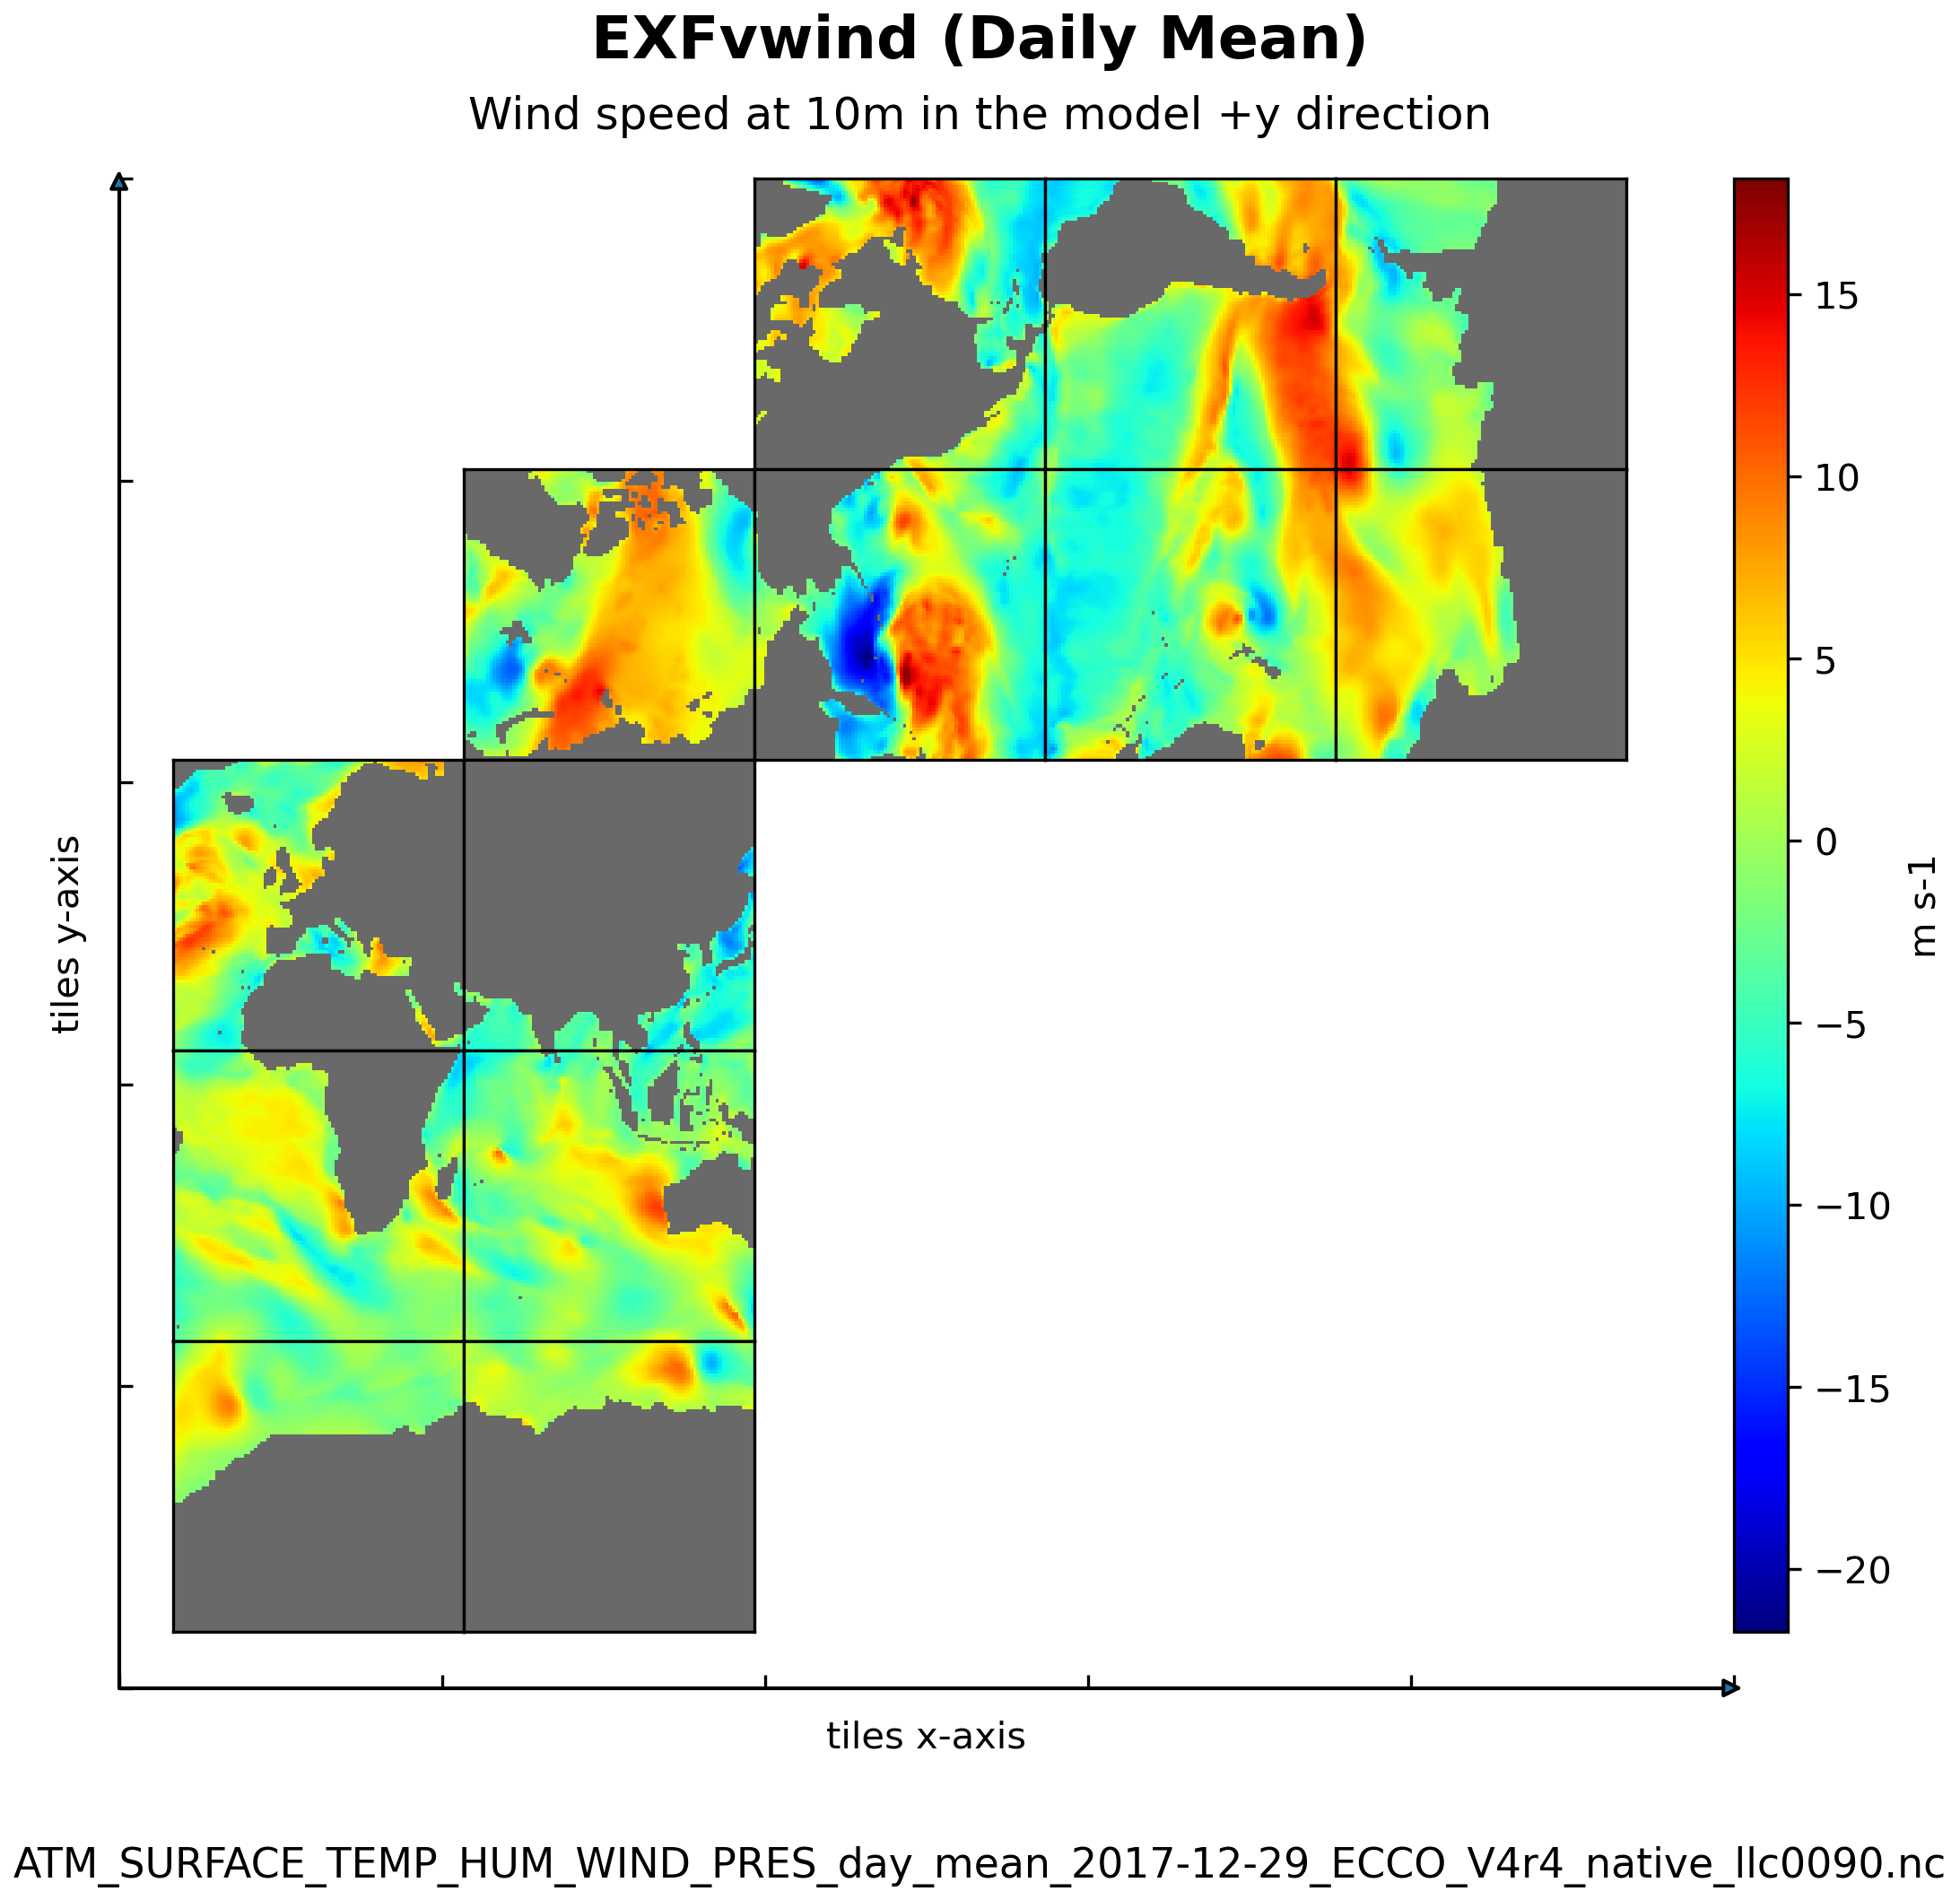
\includegraphics[scale=0.5]{../images/plots/native_plots/Atmosphere_Surface_Temperature_Humidity_Wind_and_Pressure/EXFvwind.png}
\caption{\\Dataset: ATM\_SURFACE\_TEMP\_HUM\_WIND\_PRES\\Variable: EXFvwind}
\label{tab:table-ATM_SURFACE_TEMP_HUM_WIND_PRES_EXFvwind-Plot}
\end{figure}
\pagebreak
\subsubsection{Native Variable EXFwspee}
\begin{longtable}{|p{0.06\textwidth}|p{0.41\textwidth}|p{0.39\textwidth}|p{0.06\textwidth}|}
\caption{CDL description of ATM\_SURFACE\_TEMP\_HUM\_WIND\_PRES's EXFwspee variable}
\label{tab:table-ATM_SURFACE_TEMP_HUM_WIND_PRES_EXFwspee} \\ 
\hline \endhead \hline \endfoot
\rowcolor{lightgray} \textbf{Storage Type} & \textbf{Variable Name} & \textbf{Description} & \textbf{Unit} \\ \hline
float32 & EXFwspee & Wind speed & m s-1 \\ \hline
\rowcolor{lightgray}  \multicolumn{4}{|p{1.00\textwidth}|}{\textbf{CDL Description}} \\ \hline
\multicolumn{4}{|p{1.00\textwidth}|}{\makecell{\parbox{1\textwidth}{float32 EXFwspee(time, tile, j, i)\\
\hspace*{0.5cm}EXFwspee: \_FillValue = 9.96921e+36\\
\hspace*{0.5cm}EXFwspee: long\_name = Wind speed\\
\hspace*{0.5cm}EXFwspee: units = m s: 1\\
\hspace*{0.5cm}EXFwspee: coverage\_content\_type = modelResult\\
\hspace*{0.5cm}EXFwspee: standard\_name = wind\_speed\\
\hspace*{0.5cm}EXFwspee: coordinates = time XC YC\\
\hspace*{0.5cm}EXFwspee: valid\_min = 0.27271032333374023\\
\hspace*{0.5cm}EXFwspee: valid\_max = 45.87086486816406}}} \\ \hline
\rowcolor{lightgray} \multicolumn{4}{|p{1.00\textwidth}|}{\textbf{Comments}} \\ \hline
\multicolumn{4}{|p{1\textwidth}|}{10-m wind speed magnitude (>= 0 ) over open water. Only used for the calculation of air-sea fluxes using bulk formulae. Note: not adjusted by the ocean state estimation and not necesarily consistent with EXFuwind and EXFvwind because EXFuwind and EXFvwind are calculated from EXFtaux and EXFtauy using bulk formulae. EXFwspee != sqrt(EXFuwind**2 + EXFvwind**2.} \\ \hline
\end{longtable}

\begin{figure}[H]
\centering
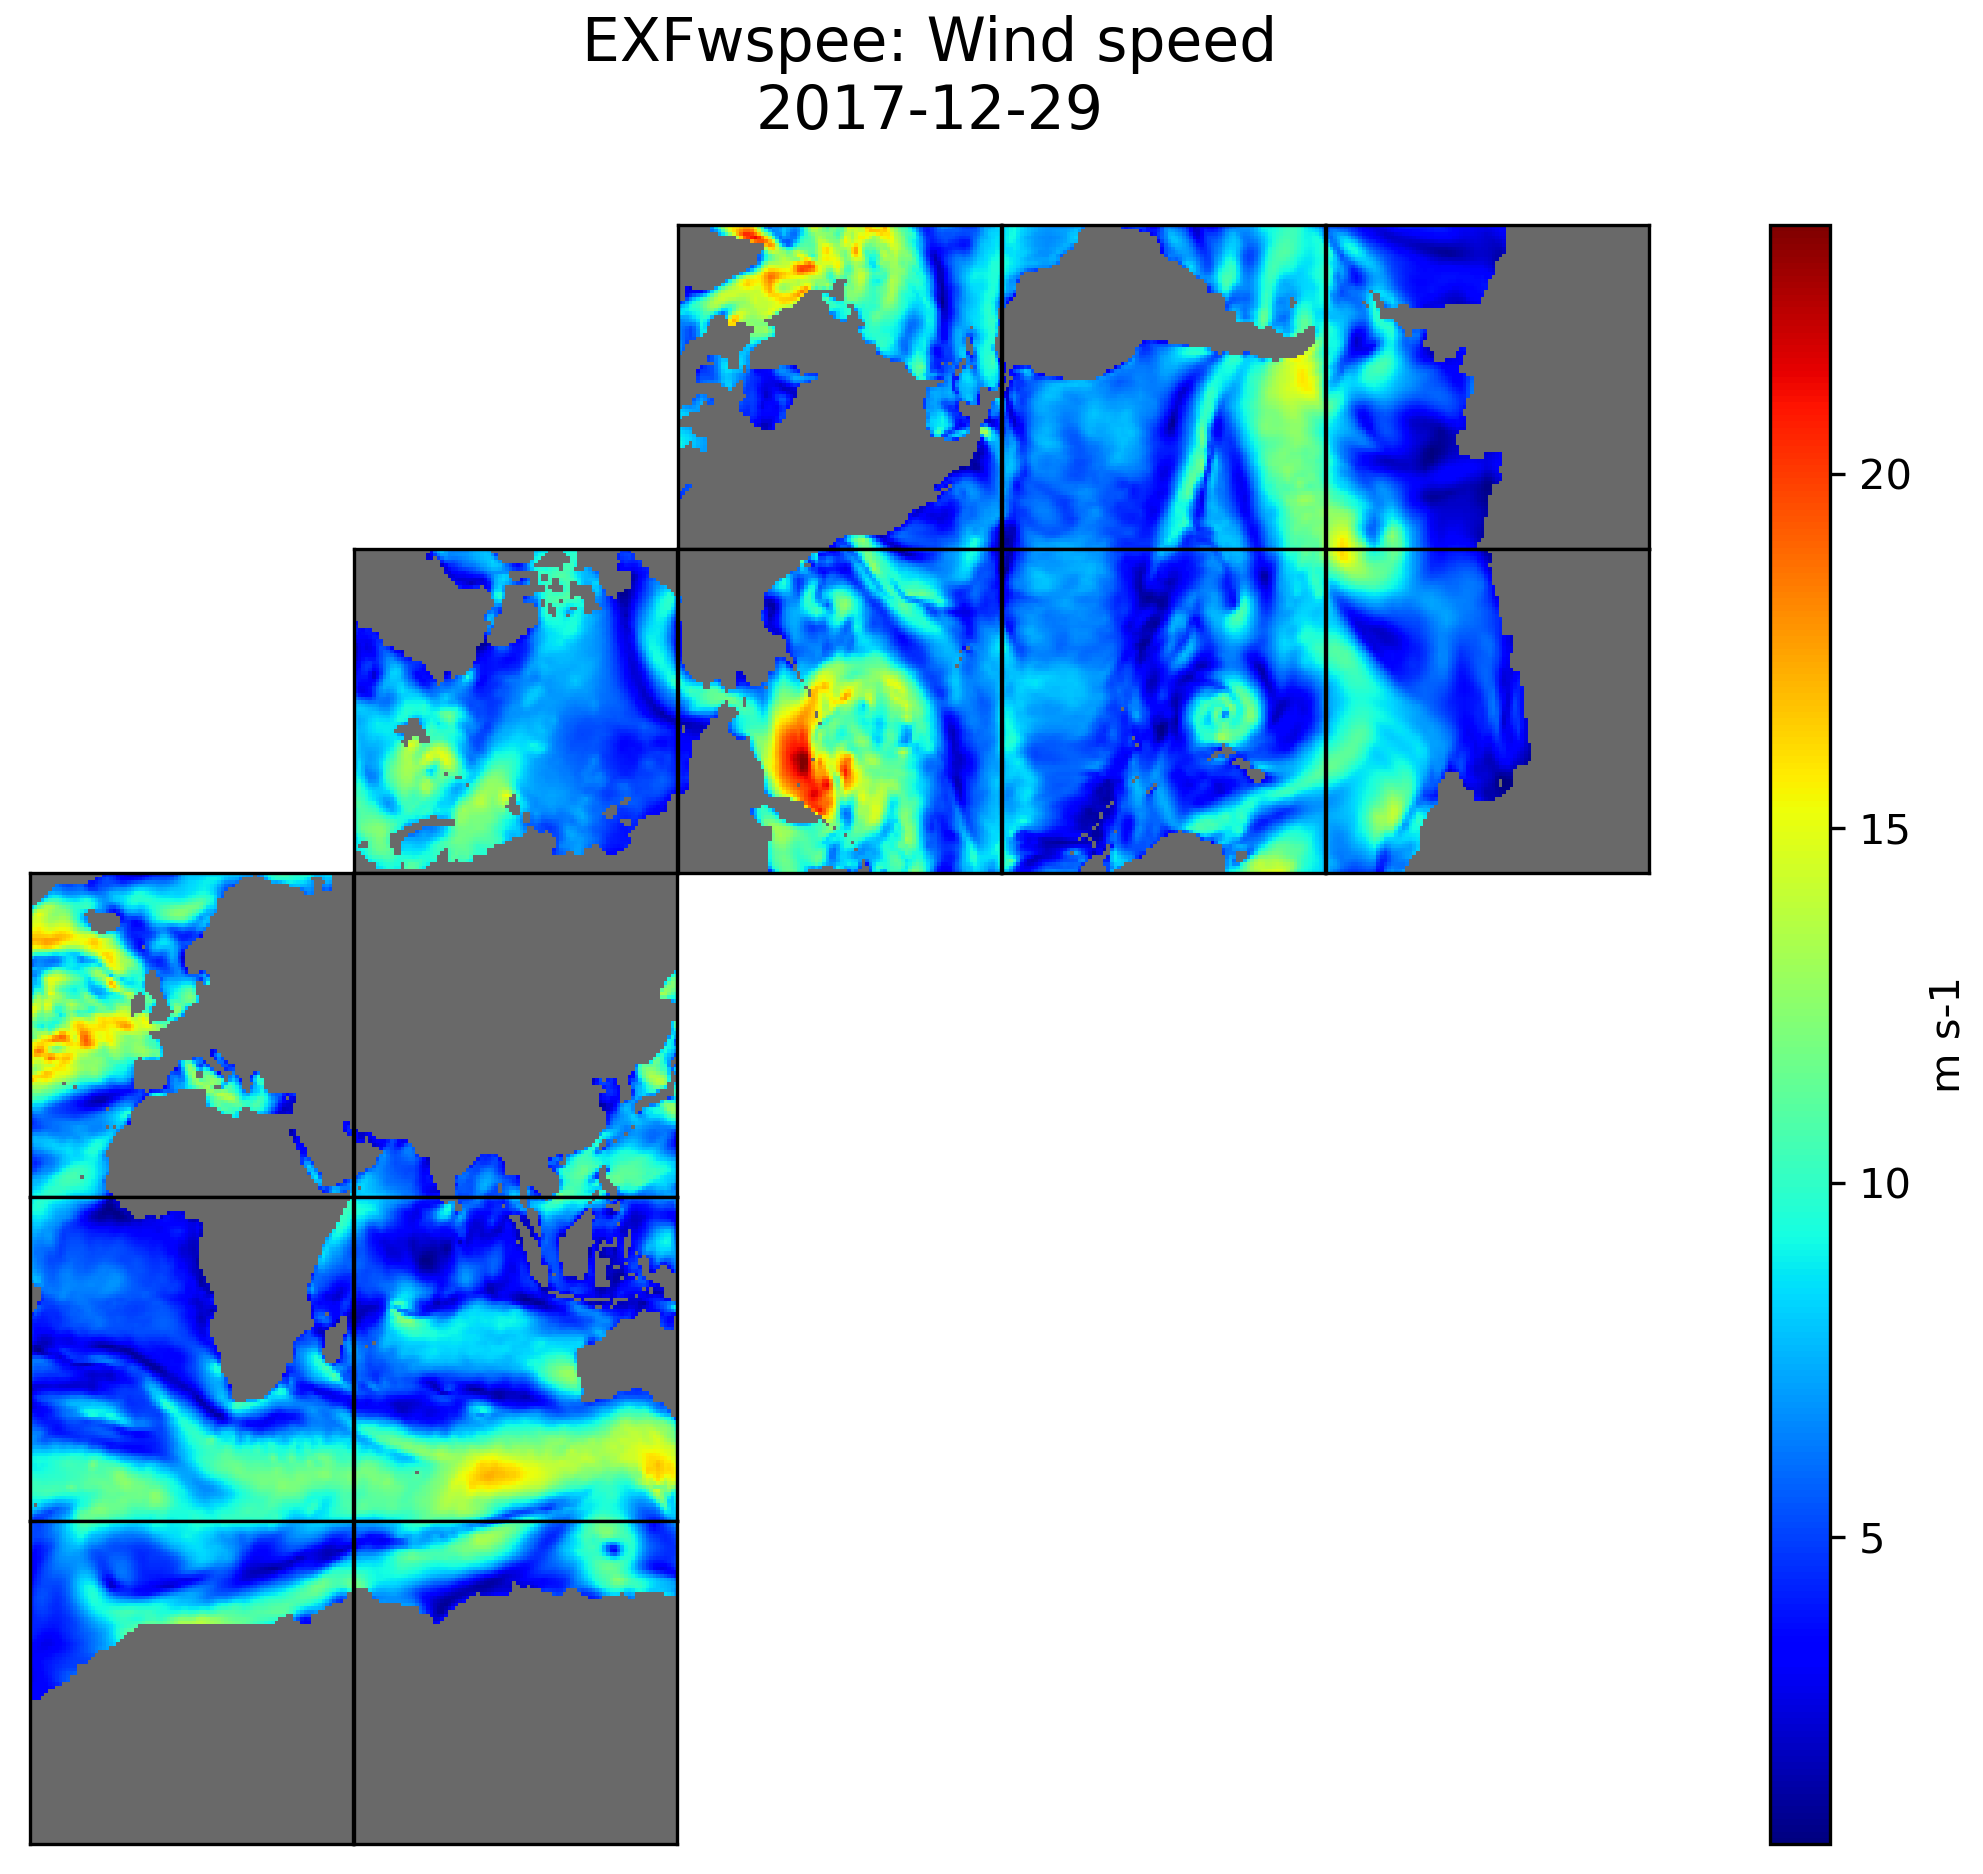
\includegraphics[scale=0.5]{../images/plots/native_plots/Atmosphere_Surface_Temperature_Humidity_Wind_and_Pressure/EXFwspee.png}
\caption{\\Dataset: ATM\_SURFACE\_TEMP\_HUM\_WIND\_PRES\\Variable: EXFwspee}
\label{tab:table-ATM_SURFACE_TEMP_HUM_WIND_PRES_EXFwspee-Plot}
\end{figure}
\pagebreak
\subsection{Native NetCDF OCEAN\_3D\_MIXING\_COEFFS}
\newp
\begin{longtable}{|p{0.1\textwidth}|p{0.5\textwidth}|}
\caption{Variables in the dataset OCEAN\_3D\_MIXING\_COEFFS\_ECCO}
\label{tab:table-OCEAN_3D_MIXING_COEFFS_ECCO-fields} \\ 
\hline \endhead \hline \endfoot
\rowcolor{lightgray} \textbf{Dataset:} & \textbf{OCEAN\_3D\_MIXING\_COEFFS\_ECCO} \\ \hline
Field: &DIFFKR \\ \hline
Field: &KAPGM \\ \hline
Field: &KAPREDI \\ \hline
\end{longtable}

\pagebreak
\subsubsection{Native Variable DIFFKR}
\begin{longtable}{|p{0.06\textwidth}|p{0.41\textwidth}|p{0.39\textwidth}|p{0.06\textwidth}|}
\caption{CDL description of OCEAN\_3D\_MIXING\_COEFFS's DIFFKR variable}
\label{tab:table-OCEAN_3D_MIXING_COEFFS_DIFFKR} \\ 
\hline \endhead \hline \endfoot
\rowcolor{lightgray} \textbf{Storage Type} & \textbf{Variable Name} & \textbf{Description} & \textbf{Unit} \\ \hline
float32 & DIFFKR & Vertical diffusivity & m2 s-1 \\ \hline
\rowcolor{lightgray}  \multicolumn{4}{|p{1.00\textwidth}|}{\textbf{CDL Description}} \\ \hline
\multicolumn{4}{|p{1.00\textwidth}|}{\makecell{\parbox{1\textwidth}{float32 DIFFKR(k, tile, j, i)\\
\hspace*{0.5cm}DIFFKR: \_FillValue = 9.96921e+36\\
\hspace*{0.5cm}DIFFKR: coverage\_content\_type = modelResult\\
\hspace*{0.5cm}DIFFKR: long\_name = Vertical diffusivity\\
\hspace*{0.5cm}DIFFKR: units = m2 s: 1\\
\hspace*{0.5cm}DIFFKR: valid\_min = 1e: 06\\
\hspace*{0.5cm}DIFFKR: valid\_max = 0.0001854995\\
\hspace*{0.5cm}DIFFKR: coordinates = Z XC YC}}} \\ \hline
\rowcolor{lightgray} \multicolumn{4}{|p{1.00\textwidth}|}{\textbf{Comments}} \\ \hline
\multicolumn{4}{|p{1\textwidth}|}{Background vertical diffusion coefficient for temperature and salinity. Total vertical diffusivity includes background diffusivity plus contributions from the GGL90 vertical mixing and the Gent-McWilliams/Redi parameterizations. Note: DIFFKR is a model control variable and has been optimized from a spatially-invariant first-guess value of 1e-5 m2 s-1.} \\ \hline
\end{longtable}

\begin{figure}[H]
\centering
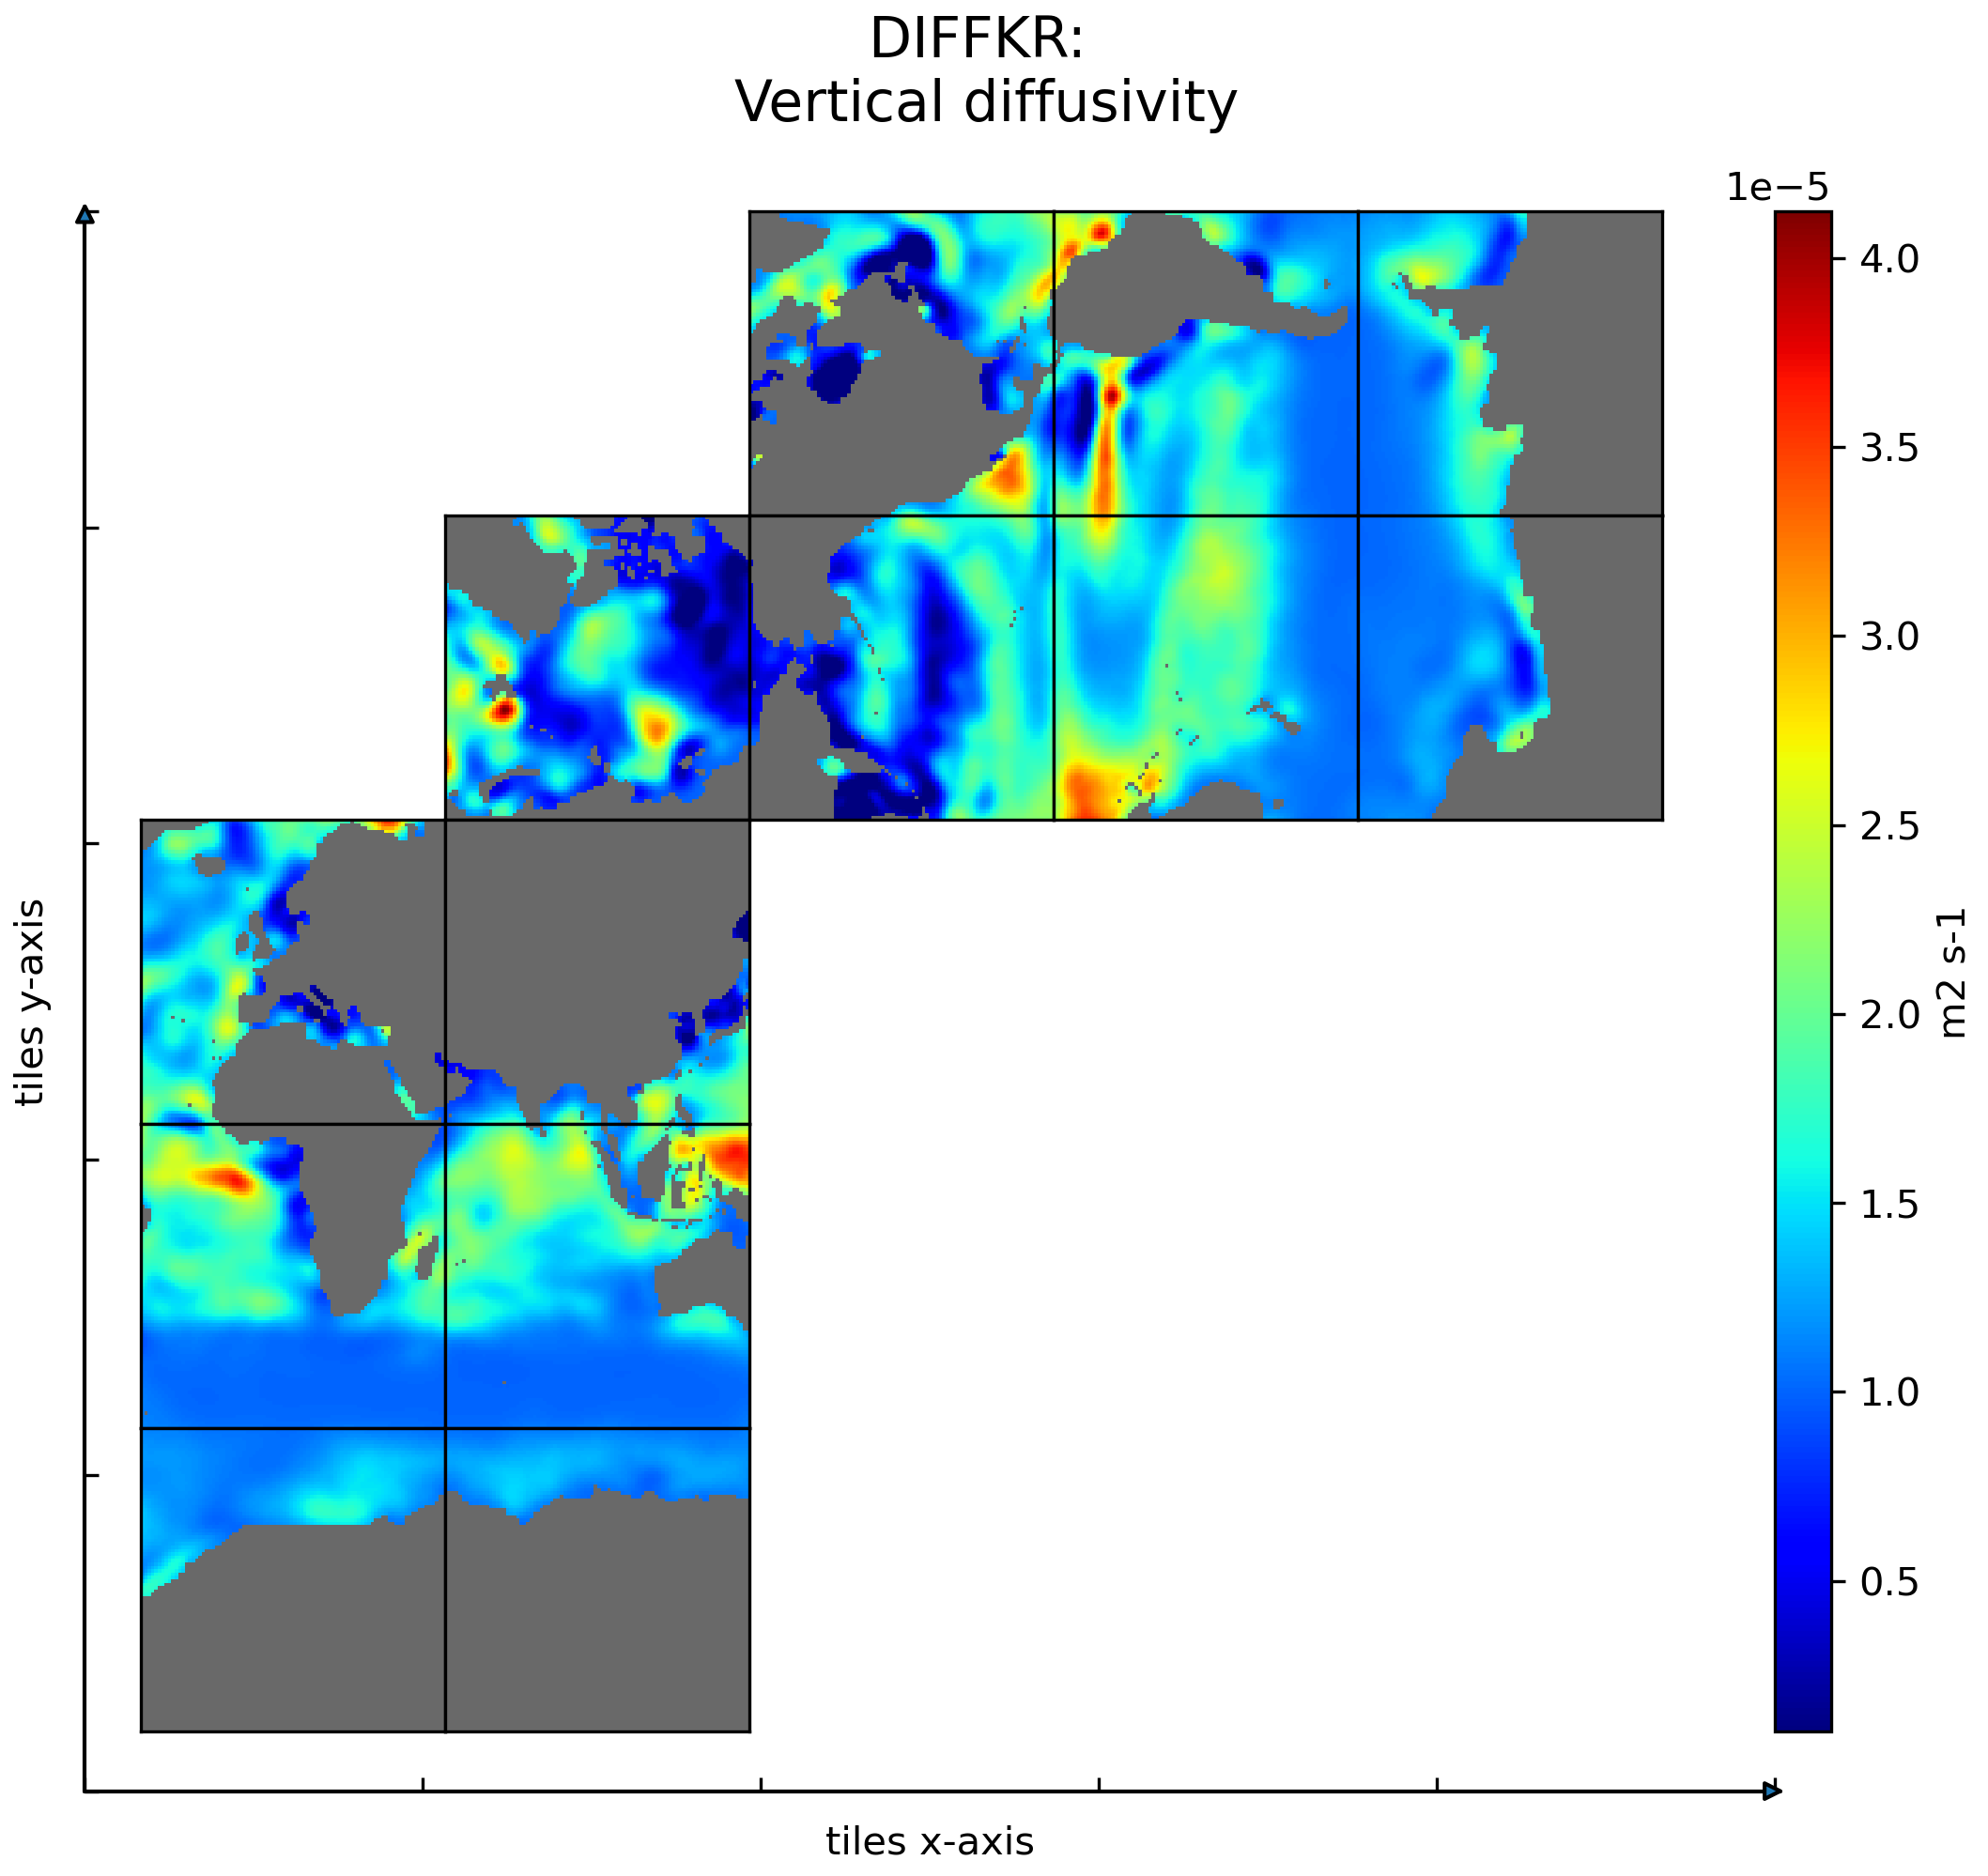
\includegraphics[scale=0.5]{../images/plots/native_plots/Ocean_3D_Gent-Mcwilliams_Redi_and_Background_Vertical_Diffusivity_Coefficients_for_the_Lat-Lon-Cap_90_(llc90)_Native_Model_Grid_(Version_4_Release_4)/DIFFKR.png}
\caption{\\Dataset: OCEAN\_3D\_MIXING\_COEFFS\\Variable: DIFFKR}
\label{tab:table-OCEAN_3D_MIXING_COEFFS_DIFFKR-Plot}
\end{figure}
\pagebreak
\subsubsection{Native Variable KAPGM}
\begin{longtable}{|p{0.06\textwidth}|p{0.41\textwidth}|p{0.39\textwidth}|p{0.06\textwidth}|}
\caption{CDL description of OCEAN\_3D\_MIXING\_COEFFS's KAPGM variable}
\label{tab:table-OCEAN_3D_MIXING_COEFFS_KAPGM} \\ 
\hline \endhead \hline \endfoot
\rowcolor{lightgray} \textbf{Storage Type} & \textbf{Variable Name} & \textbf{Description} & \textbf{Unit} \\ \hline
float32 & KAPGM & Gent-McWilliams diffusivity & m2 s-1 \\ \hline
\rowcolor{lightgray}  \multicolumn{4}{|p{1.00\textwidth}|}{\textbf{CDL Description}} \\ \hline
\multicolumn{4}{|p{1.00\textwidth}|}{\makecell{\parbox{1\textwidth}{float32 KAPGM(k, tile, j, i)\\
\hspace*{0.5cm}KAPGM: \_FillValue = 9.96921e+36\\
\hspace*{0.5cm}KAPGM: coverage\_content\_type = modelResult\\
\hspace*{0.5cm}KAPGM: long\_name = Gent: McWilliams diffusivity\\
\hspace*{0.5cm}KAPGM: units = m2 s: 1\\
\hspace*{0.5cm}KAPGM: valid\_min = 100.0\\
\hspace*{0.5cm}KAPGM: valid\_max = 10000.0\\
\hspace*{0.5cm}KAPGM: coordinates = Z XC YC}}} \\ \hline
\rowcolor{lightgray} \multicolumn{4}{|p{1.00\textwidth}|}{\textbf{Comments}} \\ \hline
\multicolumn{4}{|p{1\textwidth}|}{Gent-McWilliams diffusivity coefficient as described in Gent and McWilliams (1990, JPO). Note: KAPGM is a model control variable and has been optimized from a spatially invariant first guess of 1e3 m2 s-1.} \\ \hline
\end{longtable}

\begin{figure}[H]
\centering
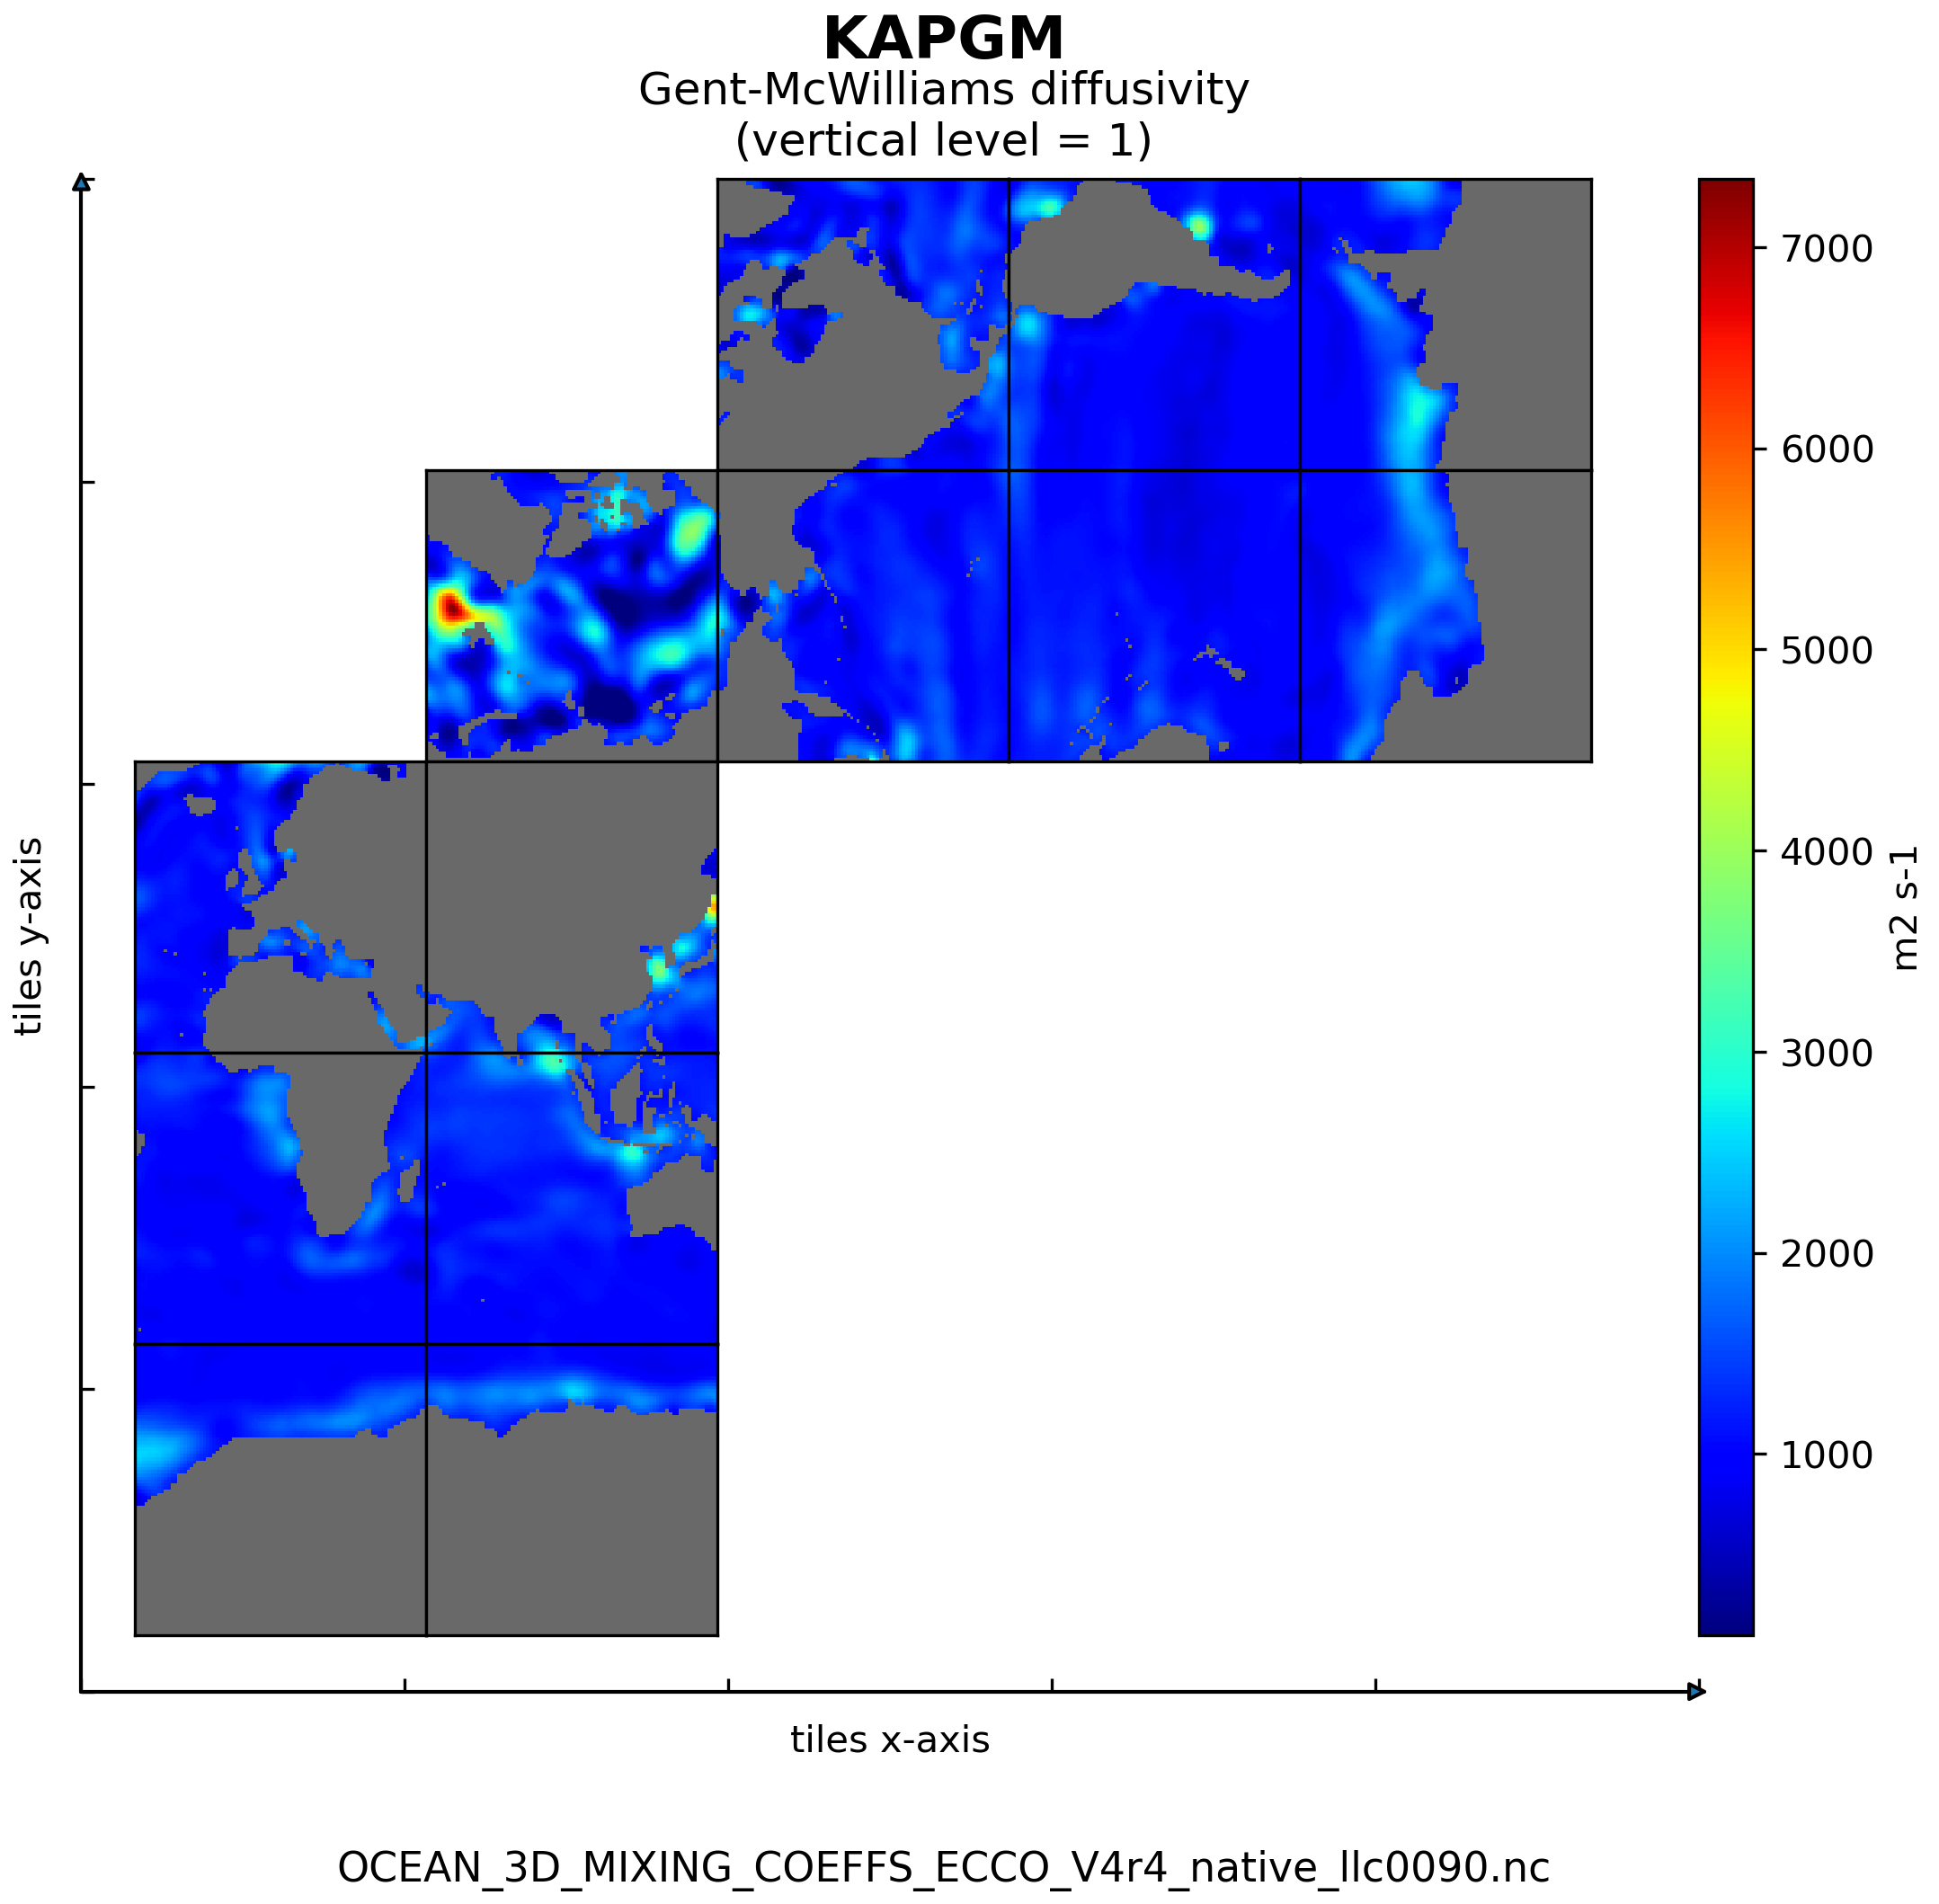
\includegraphics[scale=0.5]{../images/plots/native_plots/Ocean_3D_Gent-Mcwilliams_Redi_and_Background_Vertical_Diffusivity_Coefficients_for_the_Lat-Lon-Cap_90_(llc90)_Native_Model_Grid_(Version_4_Release_4)/KAPGM.png}
\caption{\\Dataset: OCEAN\_3D\_MIXING\_COEFFS\\Variable: KAPGM}
\label{tab:table-OCEAN_3D_MIXING_COEFFS_KAPGM-Plot}
\end{figure}
\pagebreak
\subsubsection{Native Variable KAPREDI}
\begin{longtable}{|p{0.06\textwidth}|p{0.41\textwidth}|p{0.39\textwidth}|p{0.06\textwidth}|}
\caption{CDL description of OCEAN\_3D\_MIXING\_COEFFS's KAPREDI variable}
\label{tab:table-OCEAN_3D_MIXING_COEFFS_KAPREDI} \\ 
\hline \endhead \hline \endfoot
\rowcolor{lightgray} \textbf{Storage Type} & \textbf{Variable Name} & \textbf{Description} & \textbf{Unit} \\ \hline
float32 & KAPREDI & Along-isopycnal diffusivity & m2 s-1 \\ \hline
\rowcolor{lightgray}  \multicolumn{4}{|p{1.00\textwidth}|}{\textbf{CDL Description}} \\ \hline
\multicolumn{4}{|p{1.00\textwidth}|}{\makecell{\parbox{1\textwidth}{float32 KAPREDI(k, tile, j, i)\\
\hspace*{0.5cm}KAPREDI: \_FillValue = 9.96921e+36\\
\hspace*{0.5cm}KAPREDI: coverage\_content\_type = modelResult\\
\hspace*{0.5cm}KAPREDI: long\_name = Along: isopycnal diffusivity\\
\hspace*{0.5cm}KAPREDI: units = m2 s: 1\\
\hspace*{0.5cm}KAPREDI: valid\_min = 100.0\\
\hspace*{0.5cm}KAPREDI: valid\_max = 10000.0\\
\hspace*{0.5cm}KAPREDI: coordinates = Z XC YC}}} \\ \hline
\rowcolor{lightgray} \multicolumn{4}{|p{1.00\textwidth}|}{\textbf{Comments}} \\ \hline
\multicolumn{4}{|p{1\textwidth}|}{Redi along-isopycnal diffusivity coefficient as described in Redi (1982, JPO). Note: KAPREDI is a model control variable and has been optimized from a spatially invariant first guess of 1e3 m2 s-1.} \\ \hline
\end{longtable}

\begin{figure}[H]
\centering
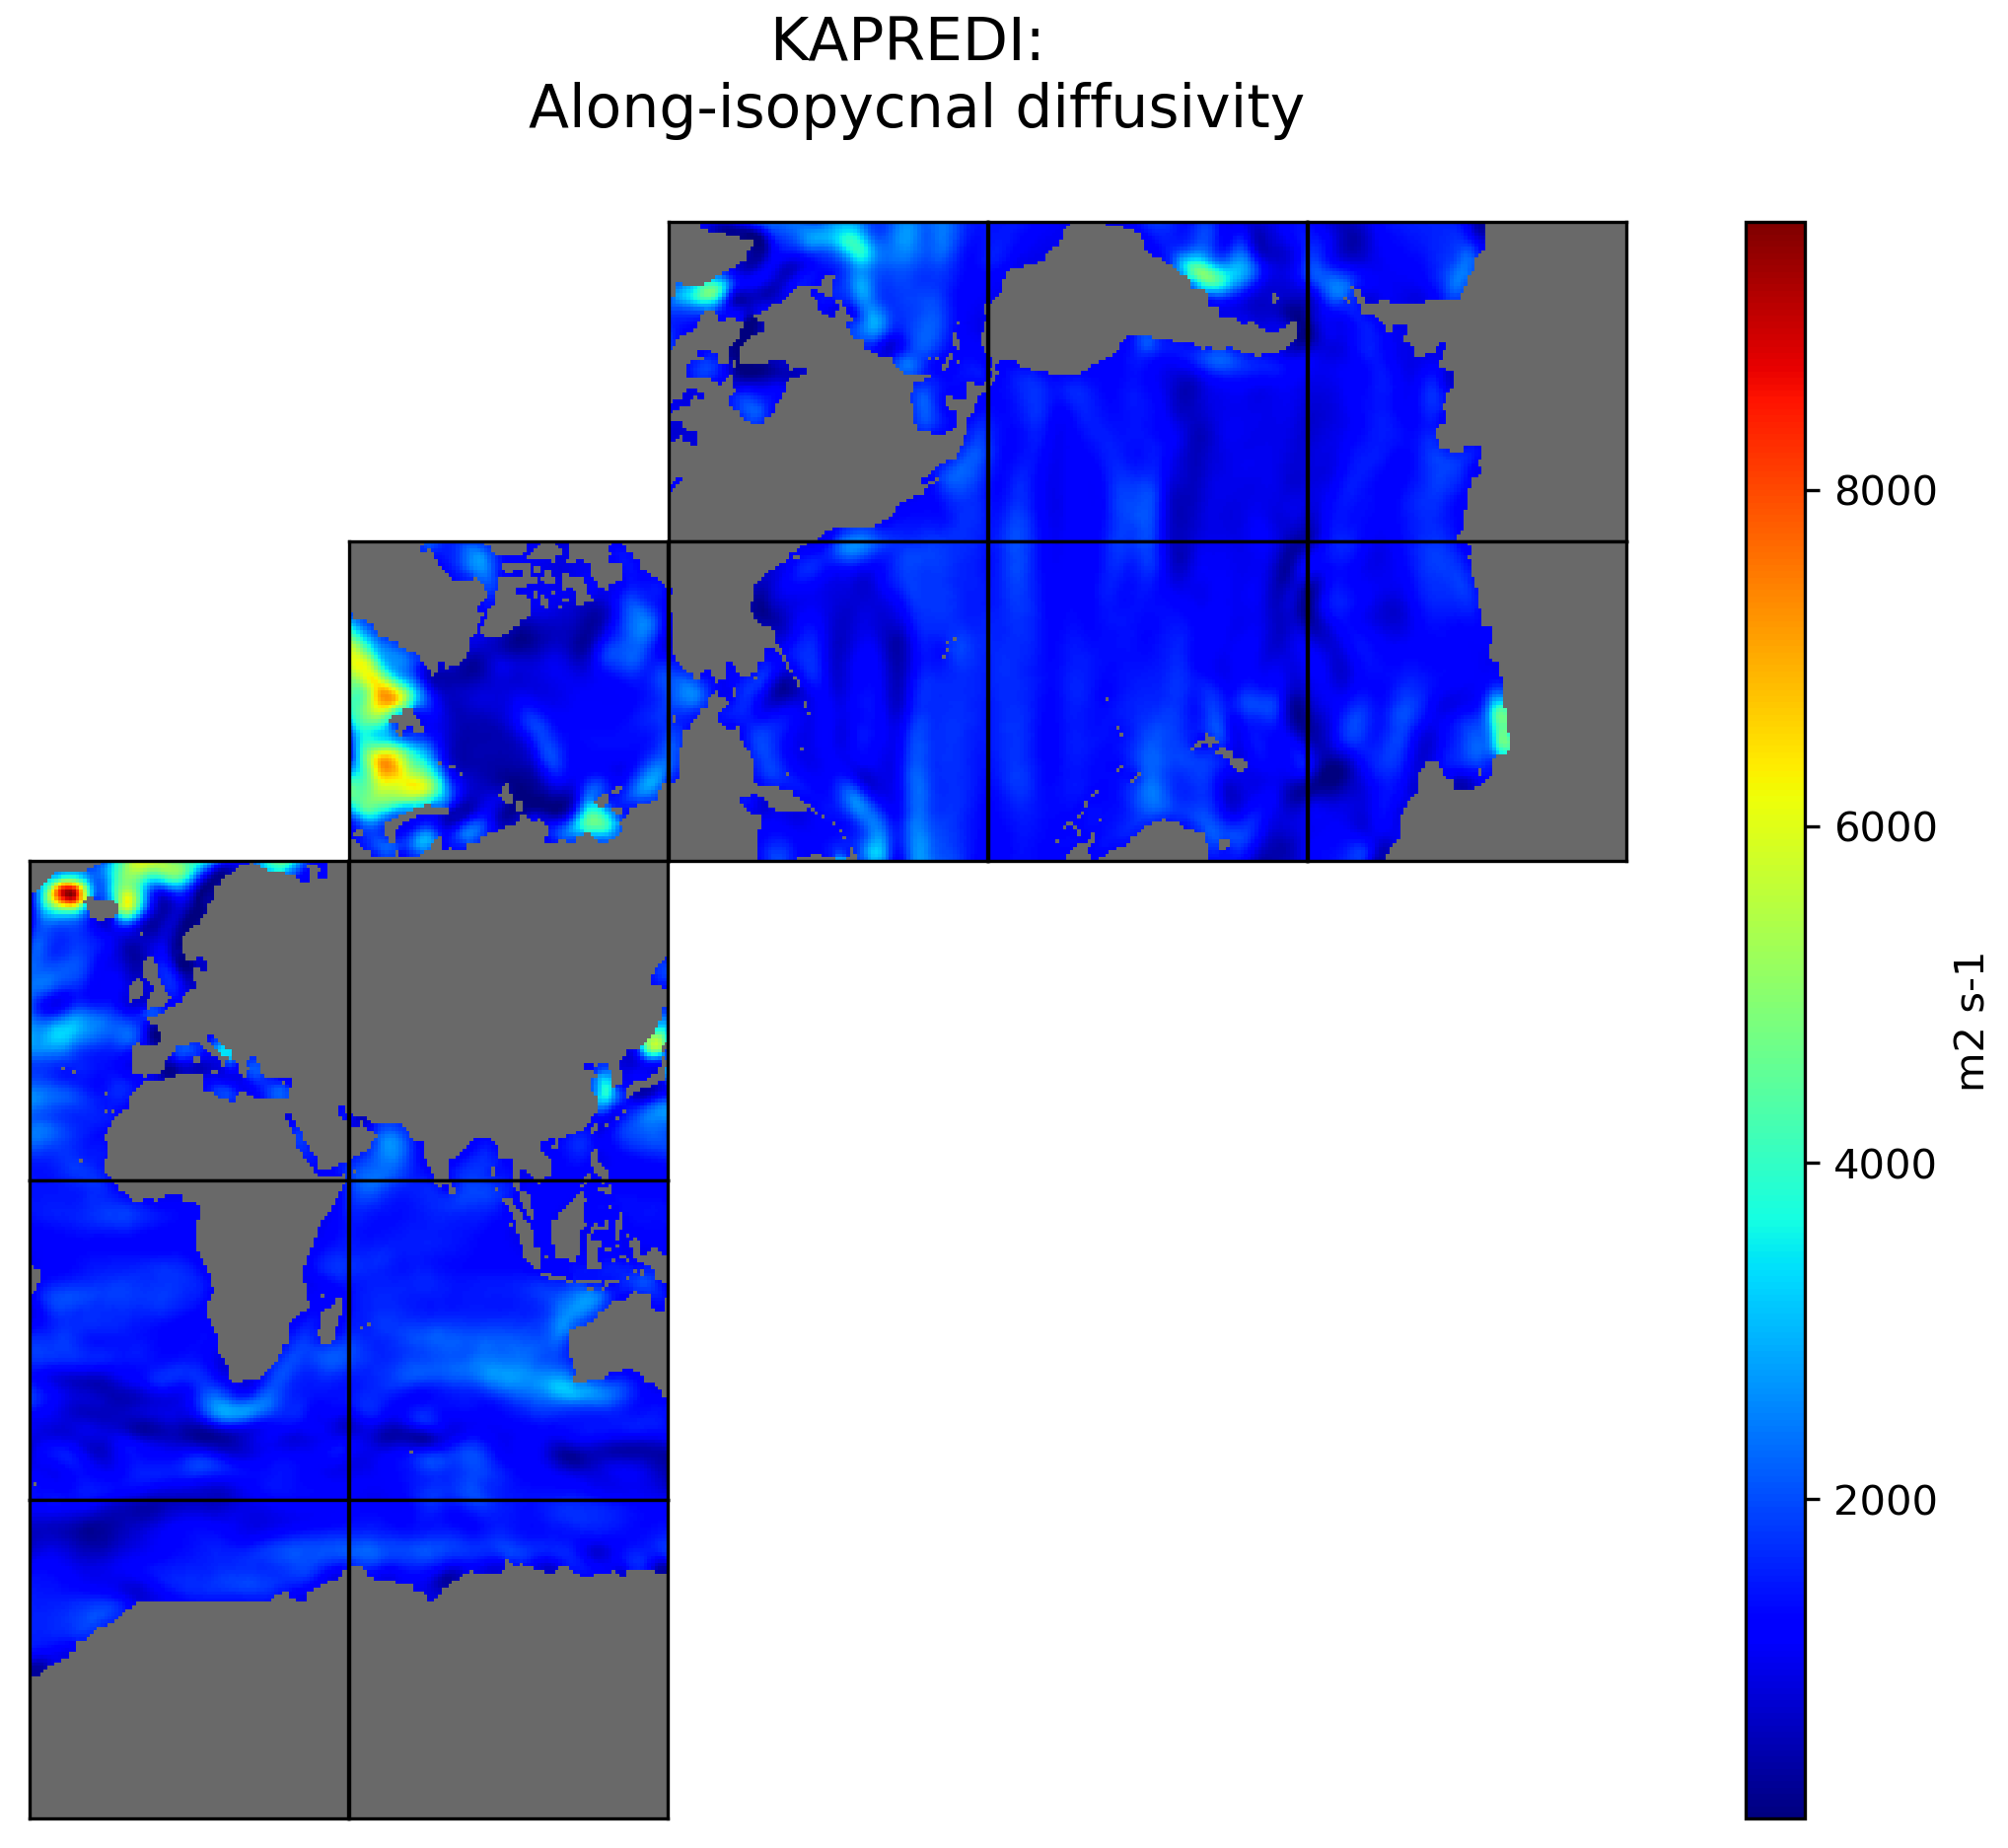
\includegraphics[scale=0.5]{../images/plots/native_plots/Ocean_3D_Gent-Mcwilliams_Redi_and_Background_Vertical_Diffusivity_Coefficients_for_the_Lat-Lon-Cap_90_(llc90)_Native_Model_Grid_(Version_4_Release_4)/KAPREDI.png}
\caption{\\Dataset: OCEAN\_3D\_MIXING\_COEFFS\\Variable: KAPREDI}
\label{tab:table-OCEAN_3D_MIXING_COEFFS_KAPREDI-Plot}
\end{figure}
\pagebreak
\subsection{Native NetCDF OCEAN\_3D\_MOMENTUM\_TEND}
\newp
\begin{longtable}{|p{0.1\textwidth}|p{0.5\textwidth}|}
\caption{Variables in the dataset OCEAN\_3D\_MOMENTUM\_TEND}
\label{tab:table-OCEAN_3D_MOMENTUM_TEND-fields} \\ 
\hline \endhead \hline \endfoot
\rowcolor{lightgray} \textbf{Dataset:} & \textbf{OCEAN\_3D\_MOMENTUM\_TEND} \\ \hline
Field: &Um\_dPHdx \\ \hline
Field: &Vm\_dPHdy \\ \hline
\end{longtable}

\pagebreak
\subsubsection{Native Variable Um\_dPHdx}
\begin{longtable}{|p{0.06\textwidth}|p{0.41\textwidth}|p{0.39\textwidth}|p{0.06\textwidth}|}
\caption{CDL description of OCEAN\_3D\_MOMENTUM\_TEND's Um\_dPHdx variable}
\label{tab:table-OCEAN_3D_MOMENTUM_TEND_Um_dPHdx} \\ 
\hline \endhead \hline \endfoot
\rowcolor{lightgray} \textbf{Storage Type} & \textbf{Variable Name} & \textbf{Description} & \textbf{Unit} \\ \hline
float32 & Um\_dPHdx & Momentum tendency in the model +x direction & m s-2 \\ \hline
\rowcolor{lightgray}  \multicolumn{4}{|p{1.00\textwidth}|}{\textbf{CDL Description}} \\ \hline
\multicolumn{4}{|p{1.00\textwidth}|}{\makecell{\parbox{1\textwidth}{float32 Um\_dPHdx(time, k, tile, j, i\_g)\\
\hspace*{0.5cm}Um\_dPHdx: \_FillValue = 9.96921e+36\\
\hspace*{0.5cm}Um\_dPHdx: long\_name = Momentum tendency in the model +x direction\\
\hspace*{0.5cm}Um\_dPHdx: units = m s: 2\\
\hspace*{0.5cm}Um\_dPHdx: mate = Vm\_dPHdy\\
\hspace*{0.5cm}Um\_dPHdx: coverage\_content\_type = modelResult\\
\hspace*{0.5cm}Um\_dPHdx: coordinates = time Z\\
\hspace*{0.5cm}Um\_dPHdx: valid\_min = : 0.0010651482734829187\\
\hspace*{0.5cm}Um\_dPHdx: valid\_max = 0.0011411579325795174}}} \\ \hline
\rowcolor{lightgray} \multicolumn{4}{|p{1.00\textwidth}|}{\textbf{Comments}} \\ \hline
\multicolumn{4}{|p{1\textwidth}|}{Momentum tendency in the +x direction due to the hydrostatic pressure gradient at the 'u' face of the native model grid cell . Note: the model +x direction does not necessarily correspond to the geographical east-west direction because the x and y axes of the model's curvilinear lat-lon-cap (llc) grid have arbitrary orientations which vary within and across tiles.} \\ \hline
\end{longtable}

\begin{figure}[H]
\centering
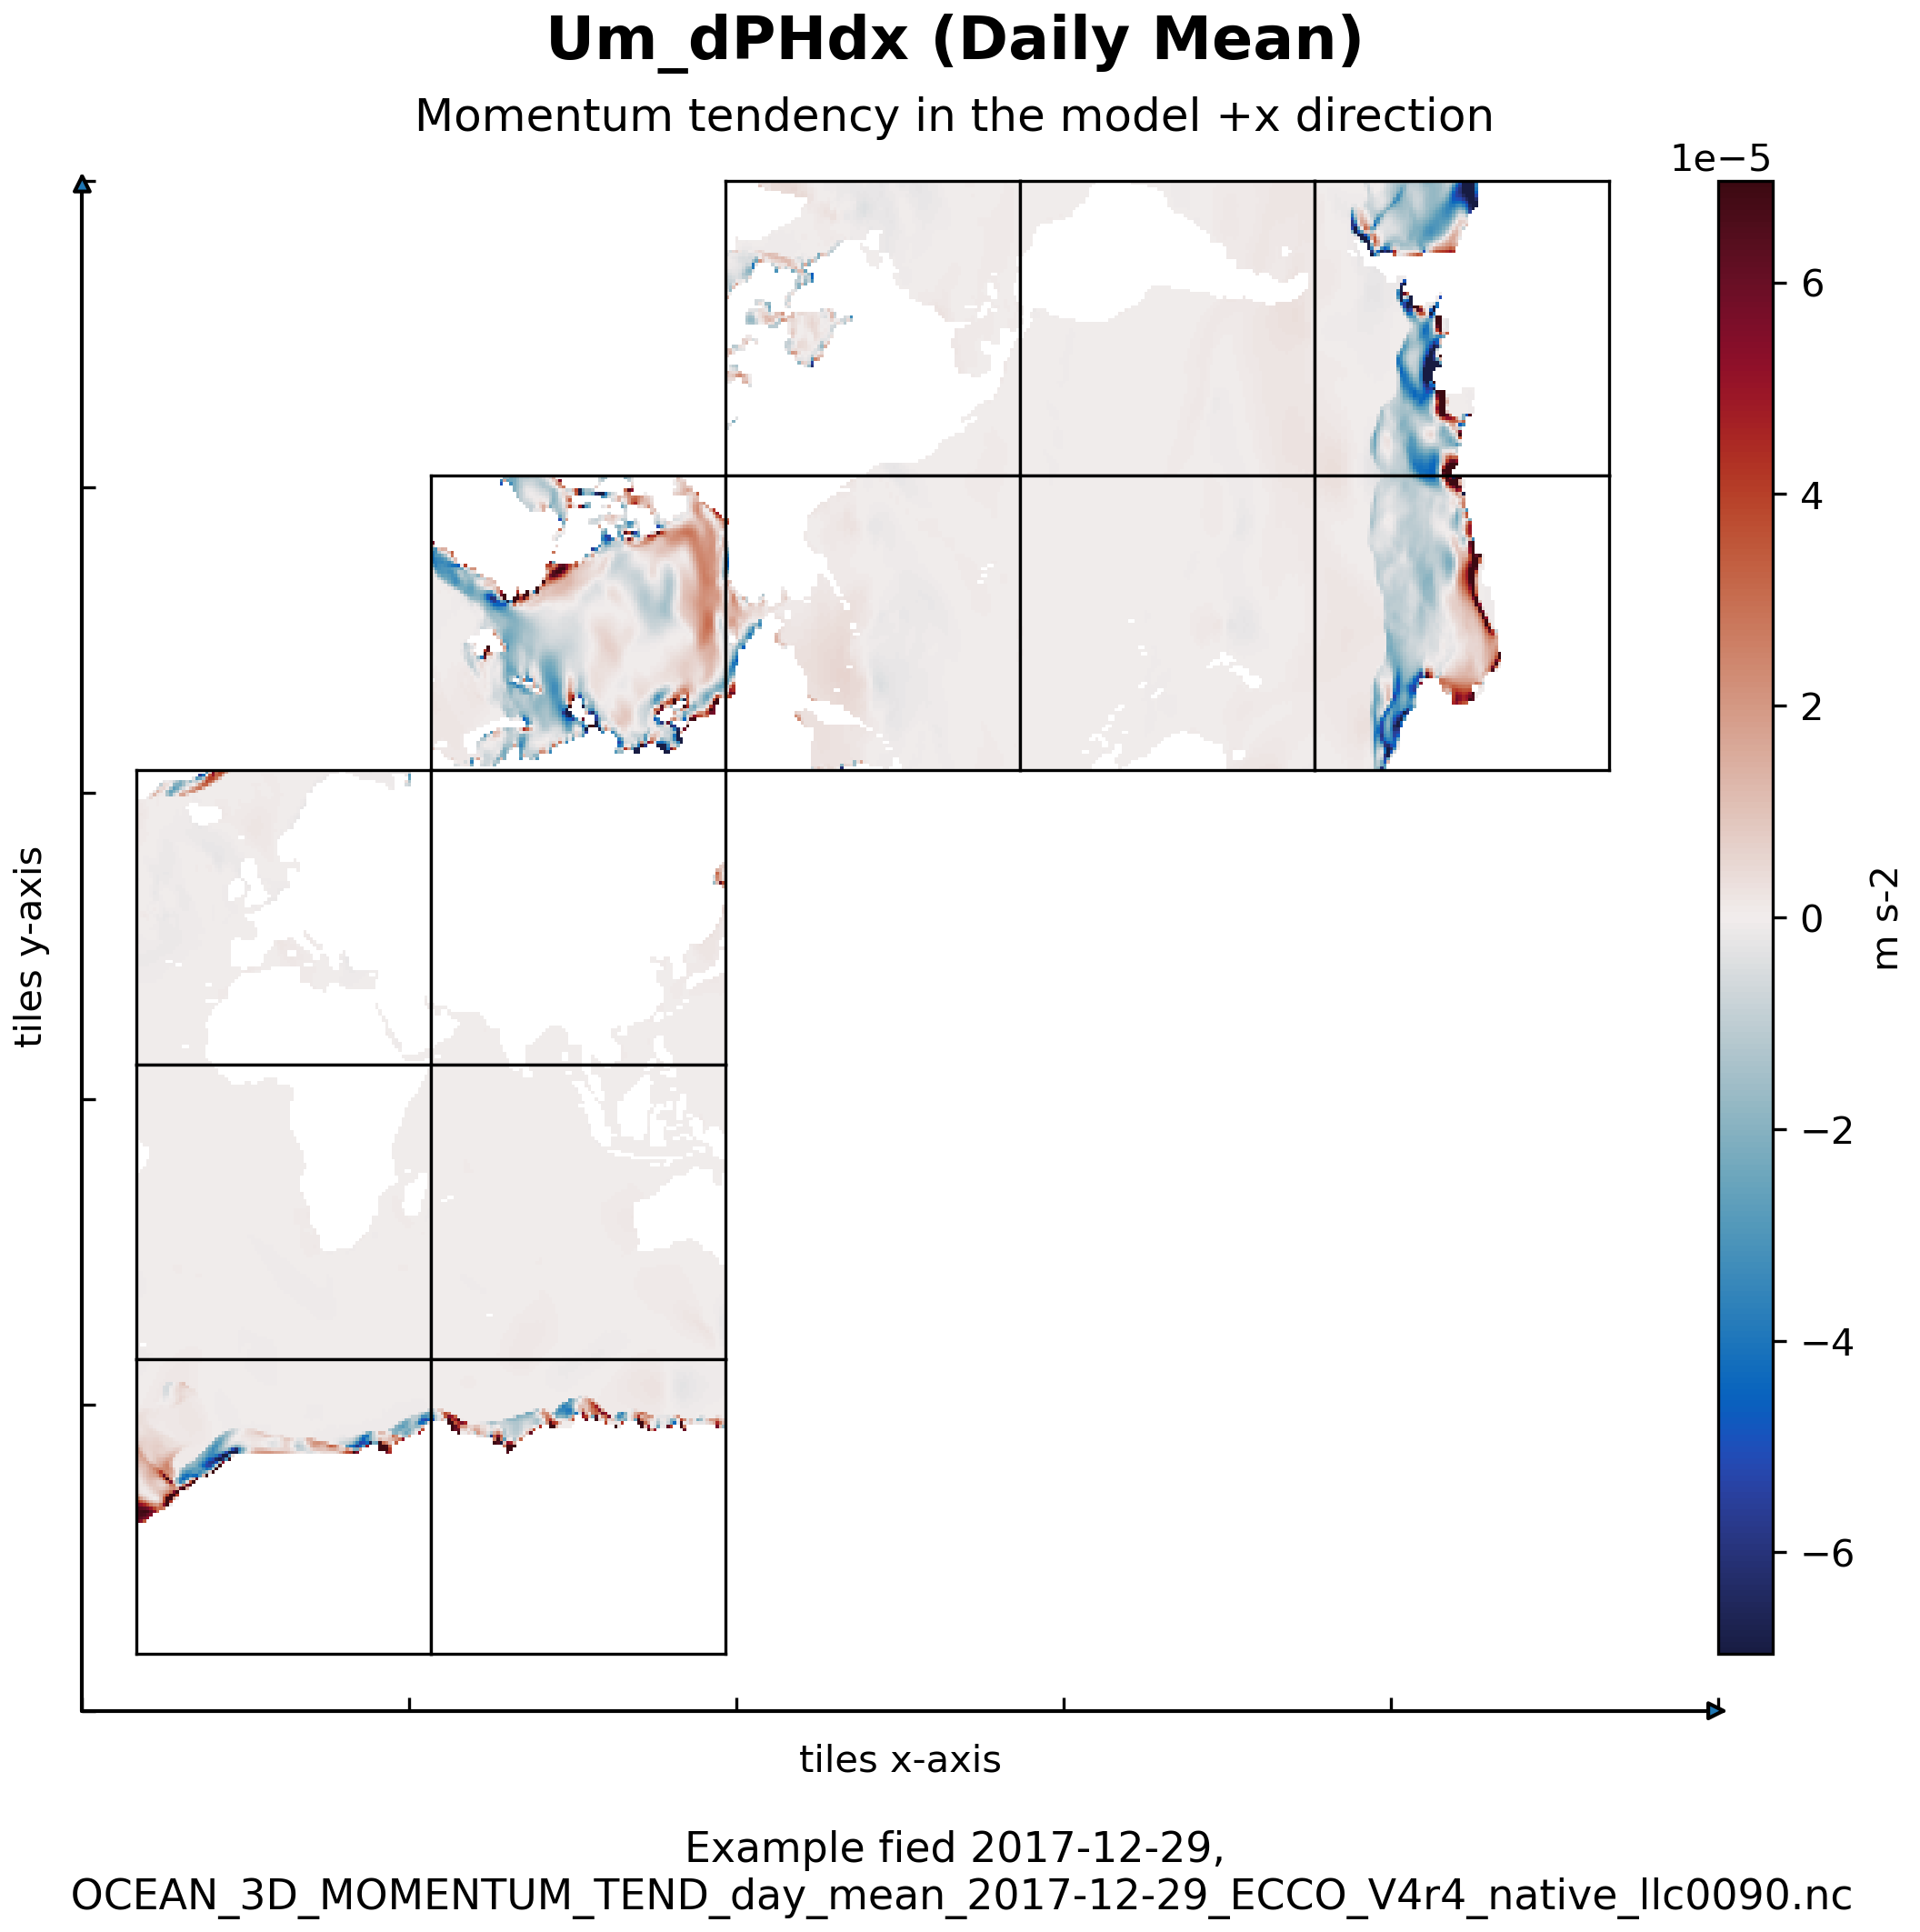
\includegraphics[scale=0.5]{../images/plots/native_plots/Ocean_Three-Dimensional_Momentum_Tendency/Um_dPHdx.png}
\caption{\\Dataset: OCEAN\_3D\_MOMENTUM\_TEND\\Variable: Um\_dPHdx}
\label{tab:table-OCEAN_3D_MOMENTUM_TEND_Um_dPHdx-Plot}
\end{figure}
\pagebreak
\subsubsection{Native Variable Vm\_dPHdy}
\begin{longtable}{|p{0.06\textwidth}|p{0.41\textwidth}|p{0.39\textwidth}|p{0.06\textwidth}|}
\caption{CDL description of OCEAN\_3D\_MOMENTUM\_TEND's Vm\_dPHdy variable}
\label{tab:table-OCEAN_3D_MOMENTUM_TEND_Vm_dPHdy} \\ 
\hline \endhead \hline \endfoot
\rowcolor{lightgray} \textbf{Storage Type} & \textbf{Variable Name} & \textbf{Description} & \textbf{Unit} \\ \hline
float32 & Vm\_dPHdy & Momentum tendency in the model +y direction & m s-2 \\ \hline
\rowcolor{lightgray}  \multicolumn{4}{|p{1.00\textwidth}|}{\textbf{CDL Description}} \\ \hline
\multicolumn{4}{|p{1.00\textwidth}|}{\makecell{\parbox{1\textwidth}{float32 Vm\_dPHdy(time, k, tile, j\_g, i)\\
\hspace*{0.5cm}Vm\_dPHdy: \_FillValue = 9.96921e+36\\
\hspace*{0.5cm}Vm\_dPHdy: long\_name = Momentum tendency in the model +y direction\\
\hspace*{0.5cm}Vm\_dPHdy: units = m s: 2\\
\hspace*{0.5cm}Vm\_dPHdy: mate = Um\_dPHdx\\
\hspace*{0.5cm}Vm\_dPHdy: coverage\_content\_type = modelResult\\
\hspace*{0.5cm}Vm\_dPHdy: coordinates = time Z\\
\hspace*{0.5cm}Vm\_dPHdy: valid\_min = : 0.0015932790702208877\\
\hspace*{0.5cm}Vm\_dPHdy: valid\_max = 0.0008858146029524505}}} \\ \hline
\rowcolor{lightgray} \multicolumn{4}{|p{1.00\textwidth}|}{\textbf{Comments}} \\ \hline
\multicolumn{4}{|p{1\textwidth}|}{Momentum tendency in the +y direction due to the hydrostatic pressure gradient at the 'v' face of the native model grid cell . Note: the model +y direction does not necessarily correspond to the geographical north-south direction because the x and y axes of the model's curvilinear lat-lon-cap (llc) grid have arbitrary orientations which vary within and across tiles.} \\ \hline
\end{longtable}

\begin{figure}[H]
\centering
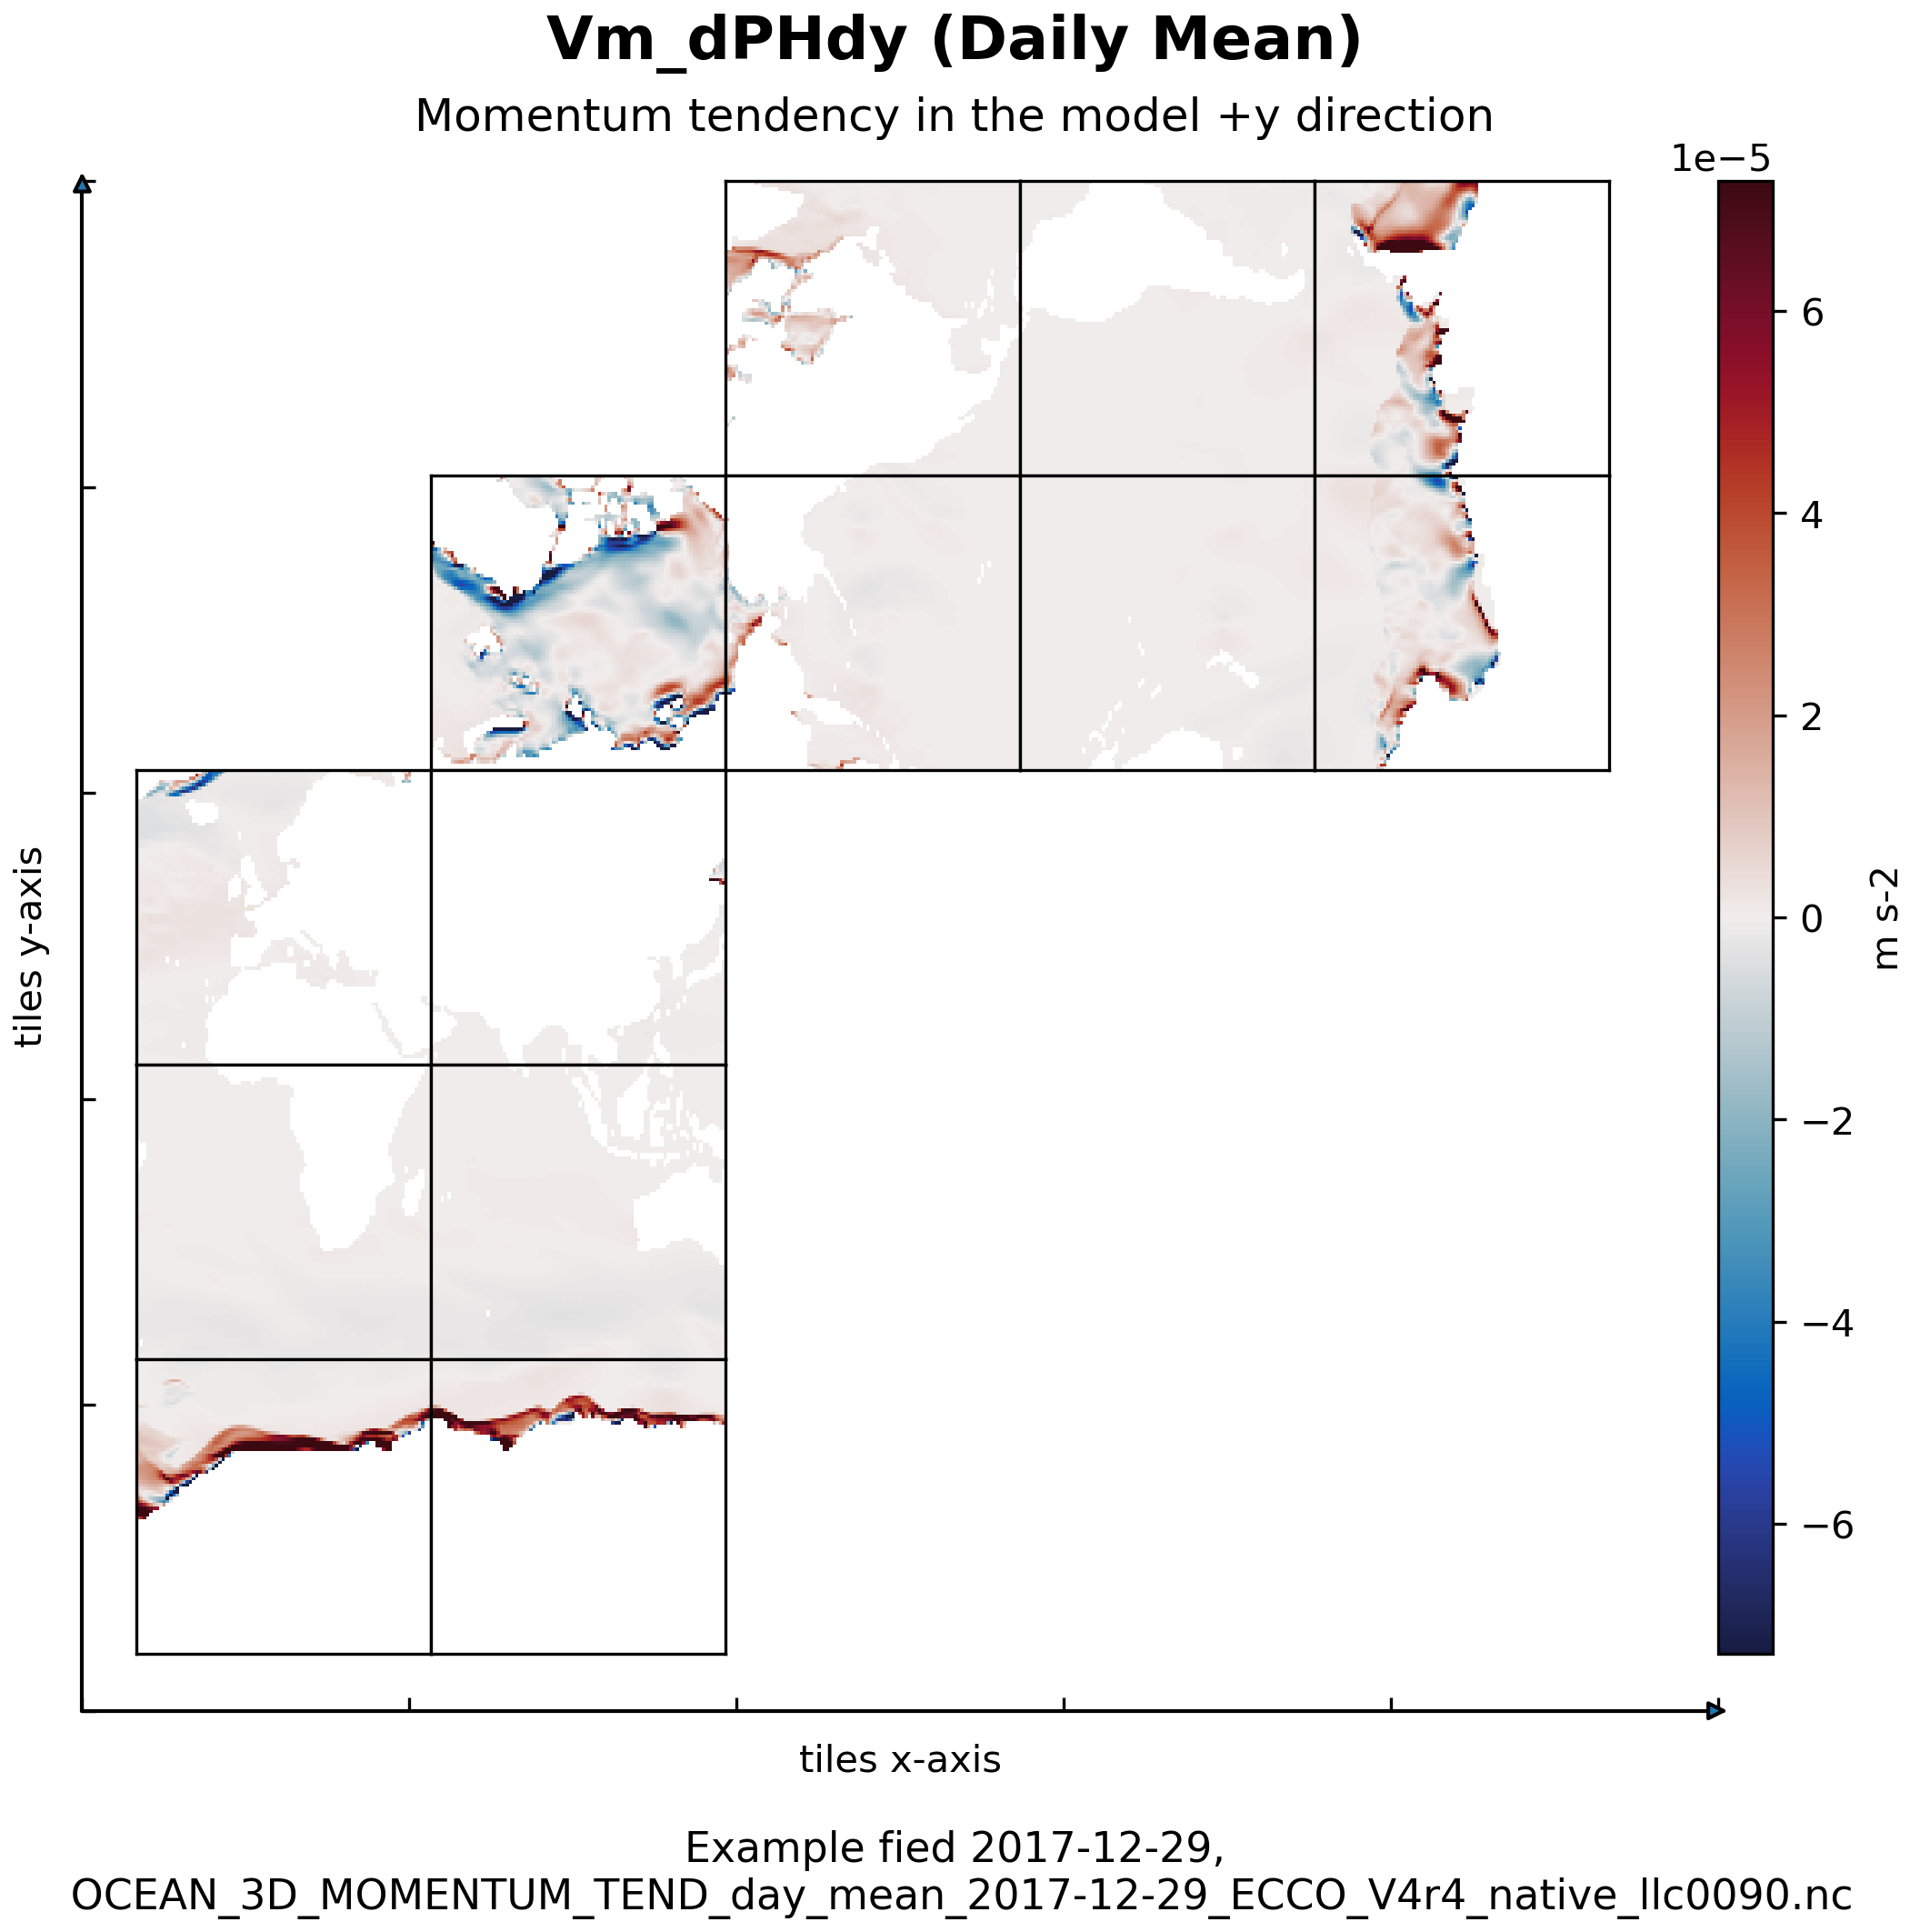
\includegraphics[scale=0.5]{../images/plots/native_plots/Ocean_Three-Dimensional_Momentum_Tendency/Vm_dPHdy.png}
\caption{\\Dataset: OCEAN\_3D\_MOMENTUM\_TEND\\Variable: Vm\_dPHdy}
\label{tab:table-OCEAN_3D_MOMENTUM_TEND_Vm_dPHdy-Plot}
\end{figure}
\pagebreak
\subsection{Native NetCDF OCEAN\_3D\_SALINITY\_FLUX}
\newp
\begin{longtable}{|p{0.1\textwidth}|p{0.5\textwidth}|}
\caption{Variables in the dataset OCEAN\_3D\_SALINITY\_FLUX}
\label{tab:table-OCEAN_3D_SALINITY_FLUX-fields} \\ 
\hline \endhead \hline \endfoot
\rowcolor{lightgray} \textbf{Dataset:} & \textbf{OCEAN\_3D\_SALINITY\_FLUX} \\ \hline
Field: &ADVx\_SLT \\ \hline
Field: &DFxE\_SLT \\ \hline
Field: &ADVy\_SLT \\ \hline
Field: &DFyE\_SLT \\ \hline
Field: &ADVr\_SLT \\ \hline
Field: &DFrE\_SLT \\ \hline
Field: &DFrI\_SLT \\ \hline
Field: &oceSPtnd \\ \hline
\end{longtable}

\pagebreak
\subsubsection{Native Variable ADVr\_SLT}
\begin{longtable}{|p{0.06\textwidth}|p{0.41\textwidth}|p{0.39\textwidth}|p{0.06\textwidth}|}
\caption{CDL description of OCEAN\_3D\_SALINITY\_FLUX's ADVr\_SLT variable}
\label{tab:table-OCEAN_3D_SALINITY_FLUX_ADVr_SLT} \\ 
\hline \endhead \hline \endfoot
\rowcolor{lightgray} \textbf{Storage Type} & \textbf{Variable Name} & \textbf{Description} & \textbf{Unit} \\ \hline
float32 & ADVr\_SLT & Vertical advective flux of salinity & 1e-3 m3 s-1 \\ \hline
\rowcolor{lightgray}  \multicolumn{4}{|p{1.00\textwidth}|}{\textbf{CDL Description}} \\ \hline
\multicolumn{4}{|p{1.00\textwidth}|}{\makecell{\parbox{1\textwidth}{float32 ADVr\_SLT(time, k\_l, tile, j, i)\\
\hspace*{0.5cm}ADVr\_SLT: \_FillValue = 9.96921e+36\\
\hspace*{0.5cm}ADVr\_SLT: long\_name = Vertical advective flux of salinity\\
\hspace*{0.5cm}ADVr\_SLT: units = 1e: 3 m3 s: 1\\
\hspace*{0.5cm}ADVr\_SLT: coverage\_content\_type = modelResult\\
\hspace*{0.5cm}ADVr\_SLT: direction = >0 decreases salinity (SALT)\\
\hspace*{0.5cm}ADVr\_SLT: coordinates = XC Zl YC time\\
\hspace*{0.5cm}ADVr\_SLT: valid\_min = : 324149856.0\\
\hspace*{0.5cm}ADVr\_SLT: valid\_max = 263294624.0}}} \\ \hline
\rowcolor{lightgray} \multicolumn{4}{|p{1.00\textwidth}|}{\textbf{Comments}} \\ \hline
\multicolumn{4}{|p{1\textwidth}|}{Vertical advective flux of salinity (SALT) in the +z direction through the top 'w' face of the tracer cell on the native model grid. Note: in the Arakawa-C grid, vertical flux quantities are staggered relative to the tracer cells with indexing such that +ADVr\_SLT(i,j,k\_l) corresponds to upward +z fluxes through the top 'w' face of the tracer cell at (i,j,k). Salinity defined using CF convention 'Sea water salinity is the salt content of sea water, often on the Practical Salinity Scale of 1978. However, the unqualified term 'salinity' is generic and does not necessarily imply any particular method of calculation. The units of salinity are dimensionless and the units attribute should normally be given as 1e-3 or 0.001 i.e. parts per thousand.' see https://cfconventions.org/Data/cf-standard-names/73/build/cf-standard-name-table.html} \\ \hline
\end{longtable}

\begin{figure}[H]
\centering
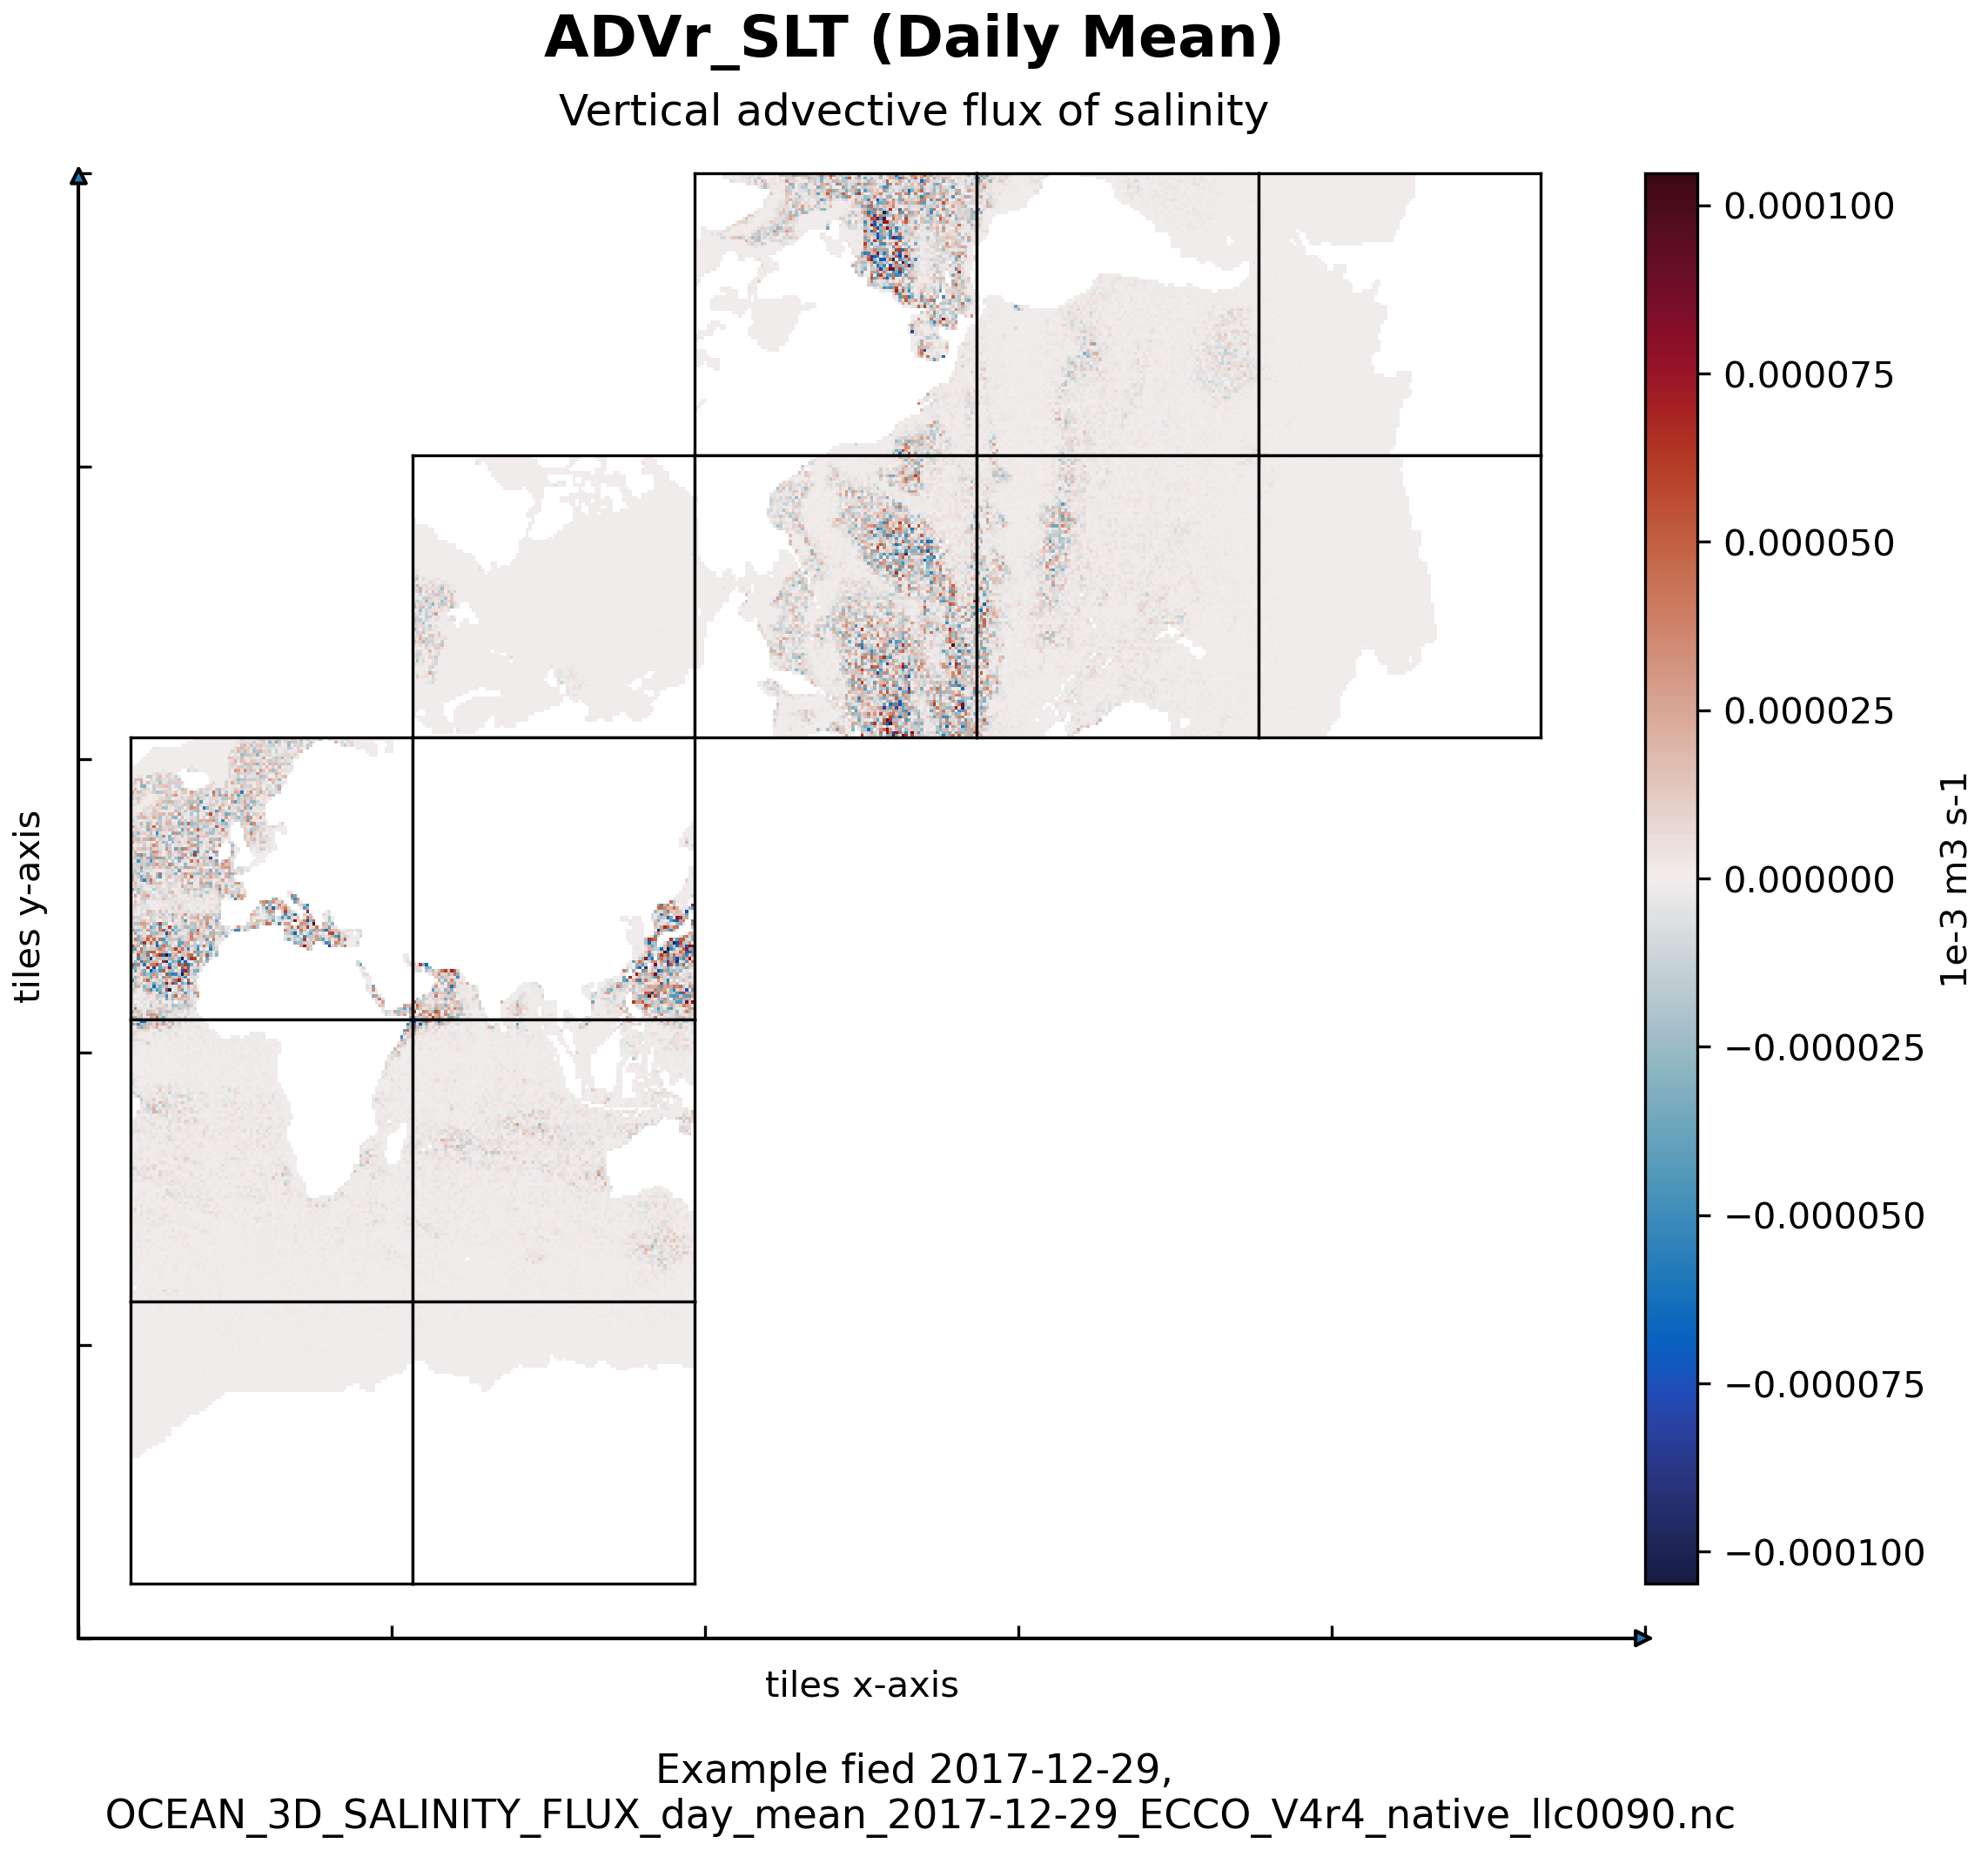
\includegraphics[scale=0.5]{../images/plots/native_plots/Ocean_Three-Dimensional_Salinity_Fluxes/ADVr_SLT.png}
\caption{\\Dataset: OCEAN\_3D\_SALINITY\_FLUX\\Variable: ADVr\_SLT}
\label{tab:table-OCEAN_3D_SALINITY_FLUX_ADVr_SLT-Plot}
\end{figure}
\pagebreak
\subsubsection{Native Variable ADVx\_SLT}
\begin{longtable}{|p{0.06\textwidth}|p{0.41\textwidth}|p{0.39\textwidth}|p{0.06\textwidth}|}
\caption{CDL description of OCEAN\_3D\_SALINITY\_FLUX's ADVx\_SLT variable}
\label{tab:table-OCEAN_3D_SALINITY_FLUX_ADVx_SLT} \\ 
\hline \endhead \hline \endfoot
\rowcolor{lightgray} \textbf{Storage Type} & \textbf{Variable Name} & \textbf{Description} & \textbf{Unit} \\ \hline
float32 & ADVx\_SLT & Lateral advective flux of salinity in the model +x direction & 1e-3 m3 s-1 \\ \hline
\rowcolor{lightgray}  \multicolumn{4}{|p{1.00\textwidth}|}{\textbf{CDL Description}} \\ \hline
\multicolumn{4}{|p{1.00\textwidth}|}{\makecell{\parbox{1\textwidth}{float32 ADVx\_SLT(time, k, tile, j, i\_g)\\
\hspace*{0.5cm}ADVx\_SLT: \_FillValue = 9.96921e+36\\
\hspace*{0.5cm}ADVx\_SLT: long\_name = Lateral advective flux of salinity in the model +x direction\\
\hspace*{0.5cm}ADVx\_SLT: units = 1e: 3 m3 s: 1\\
\hspace*{0.5cm}ADVx\_SLT: mate = ADVy\_SLT\\
\hspace*{0.5cm}ADVx\_SLT: coverage\_content\_type = modelResult\\
\hspace*{0.5cm}ADVx\_SLT: direction = >0 increases salinity (SALT)\\
\hspace*{0.5cm}ADVx\_SLT: coordinates = Z time\\
\hspace*{0.5cm}ADVx\_SLT: valid\_min = : 181830224.0\\
\hspace*{0.5cm}ADVx\_SLT: valid\_max = 260411296.0}}} \\ \hline
\rowcolor{lightgray} \multicolumn{4}{|p{1.00\textwidth}|}{\textbf{Comments}} \\ \hline
\multicolumn{4}{|p{1\textwidth}|}{Lateral advective flux of salinity (SALT) in the +x direction through the 'u' face of the tracer cell on the native model grid. Note: in the Arakawa-C grid, horizontal flux quantities are staggered relative to the tracer cells with indexing such that +ADVx\_SLT(i\_g,j,k) corresponds to +x fluxes through the 'u' face of the tracer cell at (i,j,k). Also, the model +x direction does not necessarily correspond to the geographical east-west direction because the x and y axes of the model's curvilinear lat-lon-cap (llc) grid have arbitrary orientations which vary within and across tiles. Salinity defined using CF convention 'Sea water salinity is the salt content of sea water, often on the Practical Salinity Scale of 1978. However, the unqualified term 'salinity' is generic and does not necessarily imply any particular method of calculation. The units of salinity are dimensionless and the units attribute should normally be given as 1e-3 or 0.001 i.e. parts per thousand.' see https://cfconventions.org/Data/cf-standard-names/73/build/cf-standard-name-table.html} \\ \hline
\end{longtable}

\begin{figure}[H]
\centering
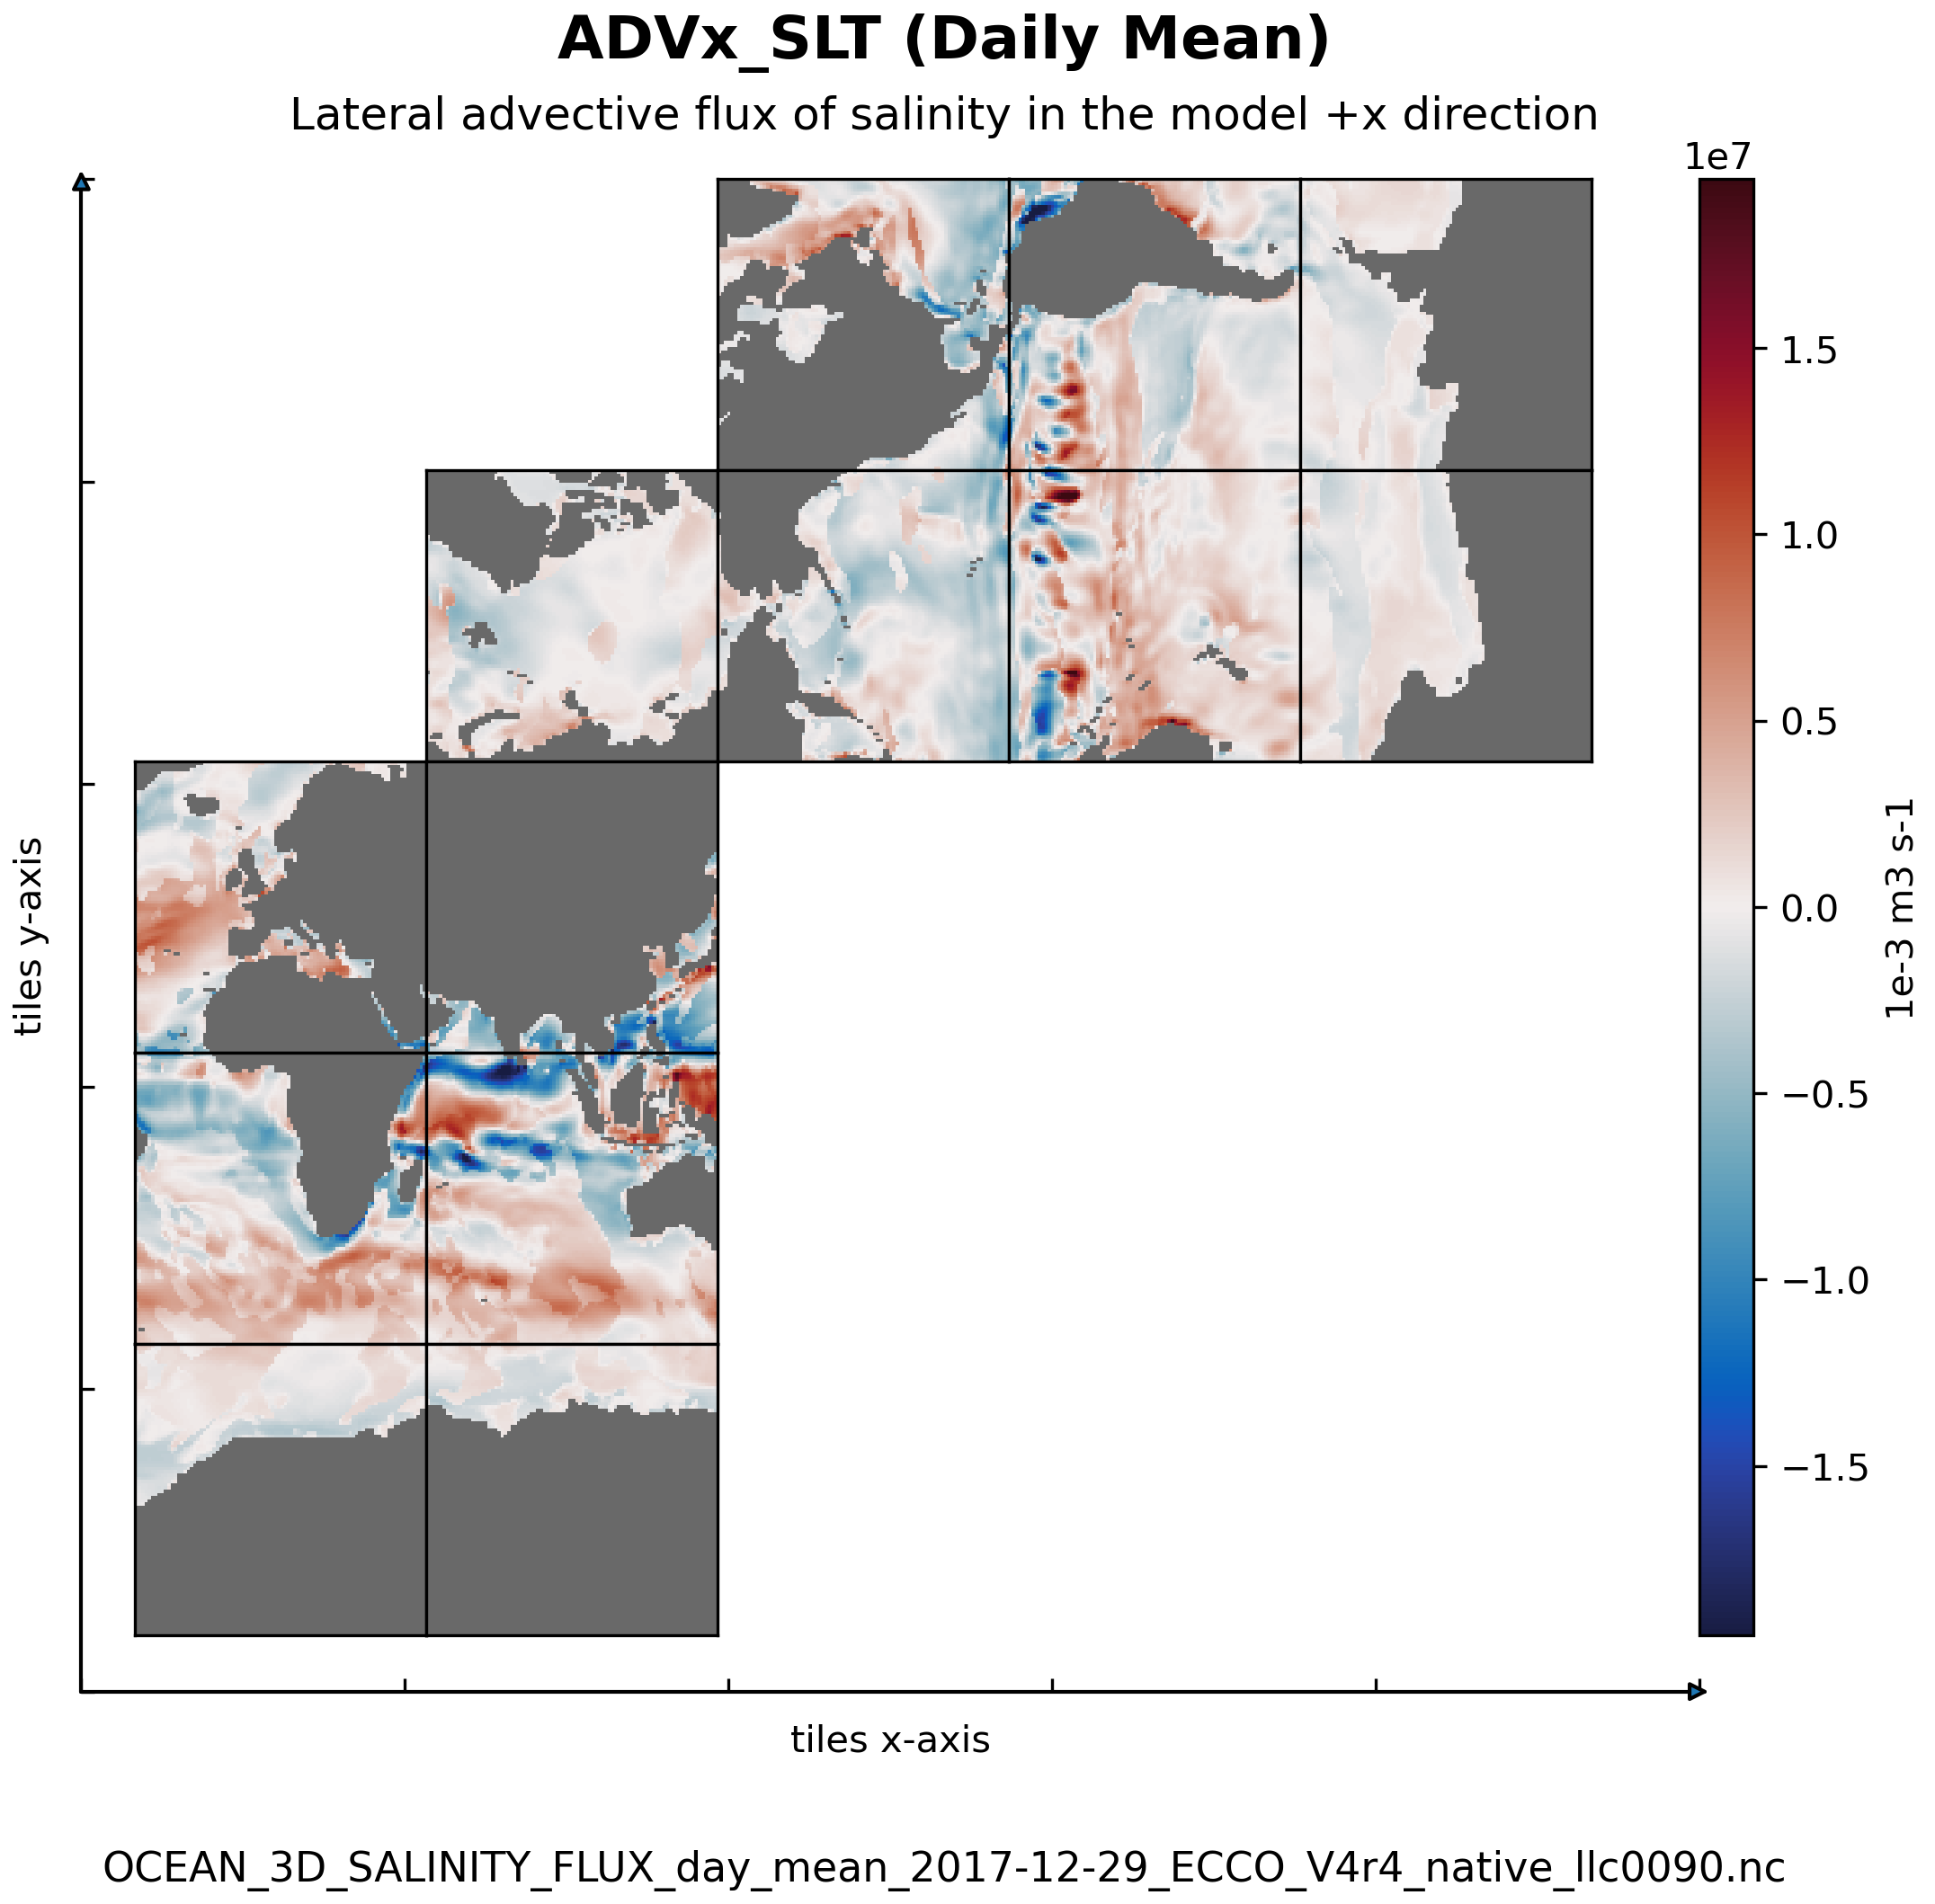
\includegraphics[scale=0.5]{../images/plots/native_plots/Ocean_Three-Dimensional_Salinity_Fluxes/ADVx_SLT.png}
\caption{\\Dataset: OCEAN\_3D\_SALINITY\_FLUX\\Variable: ADVx\_SLT}
\label{tab:table-OCEAN_3D_SALINITY_FLUX_ADVx_SLT-Plot}
\end{figure}
\pagebreak
\subsubsection{Native Variable ADVy\_SLT}
\begin{longtable}{|p{0.06\textwidth}|p{0.41\textwidth}|p{0.39\textwidth}|p{0.06\textwidth}|}
\caption{CDL description of OCEAN\_3D\_SALINITY\_FLUX's ADVy\_SLT variable}
\label{tab:table-OCEAN_3D_SALINITY_FLUX_ADVy_SLT} \\ 
\hline \endhead \hline \endfoot
\rowcolor{lightgray} \textbf{Storage Type} & \textbf{Variable Name} & \textbf{Description} & \textbf{Unit} \\ \hline
float32 & ADVy\_SLT & Lateral advective flux of salinity in the model +y direction & 1e-3 m3 s-1 \\ \hline
\rowcolor{lightgray}  \multicolumn{4}{|p{1.00\textwidth}|}{\textbf{CDL Description}} \\ \hline
\multicolumn{4}{|p{1.00\textwidth}|}{\makecell{\parbox{1\textwidth}{float32 ADVy\_SLT(time, k, tile, j\_g, i)\\
\hspace*{0.5cm}ADVy\_SLT: \_FillValue = 9.96921e+36\\
\hspace*{0.5cm}ADVy\_SLT: long\_name = Lateral advective flux of salinity in the model +y direction\\
\hspace*{0.5cm}ADVy\_SLT: units = 1e: 3 m3 s: 1\\
\hspace*{0.5cm}ADVy\_SLT: mate = ADVx\_SLT\\
\hspace*{0.5cm}ADVy\_SLT: coverage\_content\_type = modelResult\\
\hspace*{0.5cm}ADVy\_SLT: direction = >0 increases salinity (SALT)\\
\hspace*{0.5cm}ADVy\_SLT: coordinates = Z time\\
\hspace*{0.5cm}ADVy\_SLT: valid\_min = : 137905760.0\\
\hspace*{0.5cm}ADVy\_SLT: valid\_max = 164271664.0}}} \\ \hline
\rowcolor{lightgray} \multicolumn{4}{|p{1.00\textwidth}|}{\textbf{Comments}} \\ \hline
\multicolumn{4}{|p{1\textwidth}|}{Lateral advective flux of salinity (SALT) in the +y direction through the 'v' face of the tracer cell on the native model grid. Note: in the Arakawa-C grid, horizontal flux quantities are staggered relative to the tracer cells with indexing such that +ADVy\_SLT(i,j\_g,k) corresponds to +y fluxes through the 'v' face of the tracer cell at (i,j,k). Also, the model +y direction does not necessarily correspond to the geographical north-south direction because the x and y axes of the model's curvilinear lat-lon-cap (llc) grid have arbitrary orientations which vary within and across tiles. Salinity defined using CF convention 'Sea water salinity is the salt content of sea water, often on the Practical Salinity Scale of 1978. However, the unqualified term 'salinity' is generic and does not necessarily imply any particular method of calculation. The units of salinity are dimensionless and the units attribute should normally be given as 1e-3 or 0.001 i.e. parts per thousand.' see https://cfconventions.org/Data/cf-standard-names/73/build/cf-standard-name-table.html} \\ \hline
\end{longtable}

\begin{figure}[H]
\centering
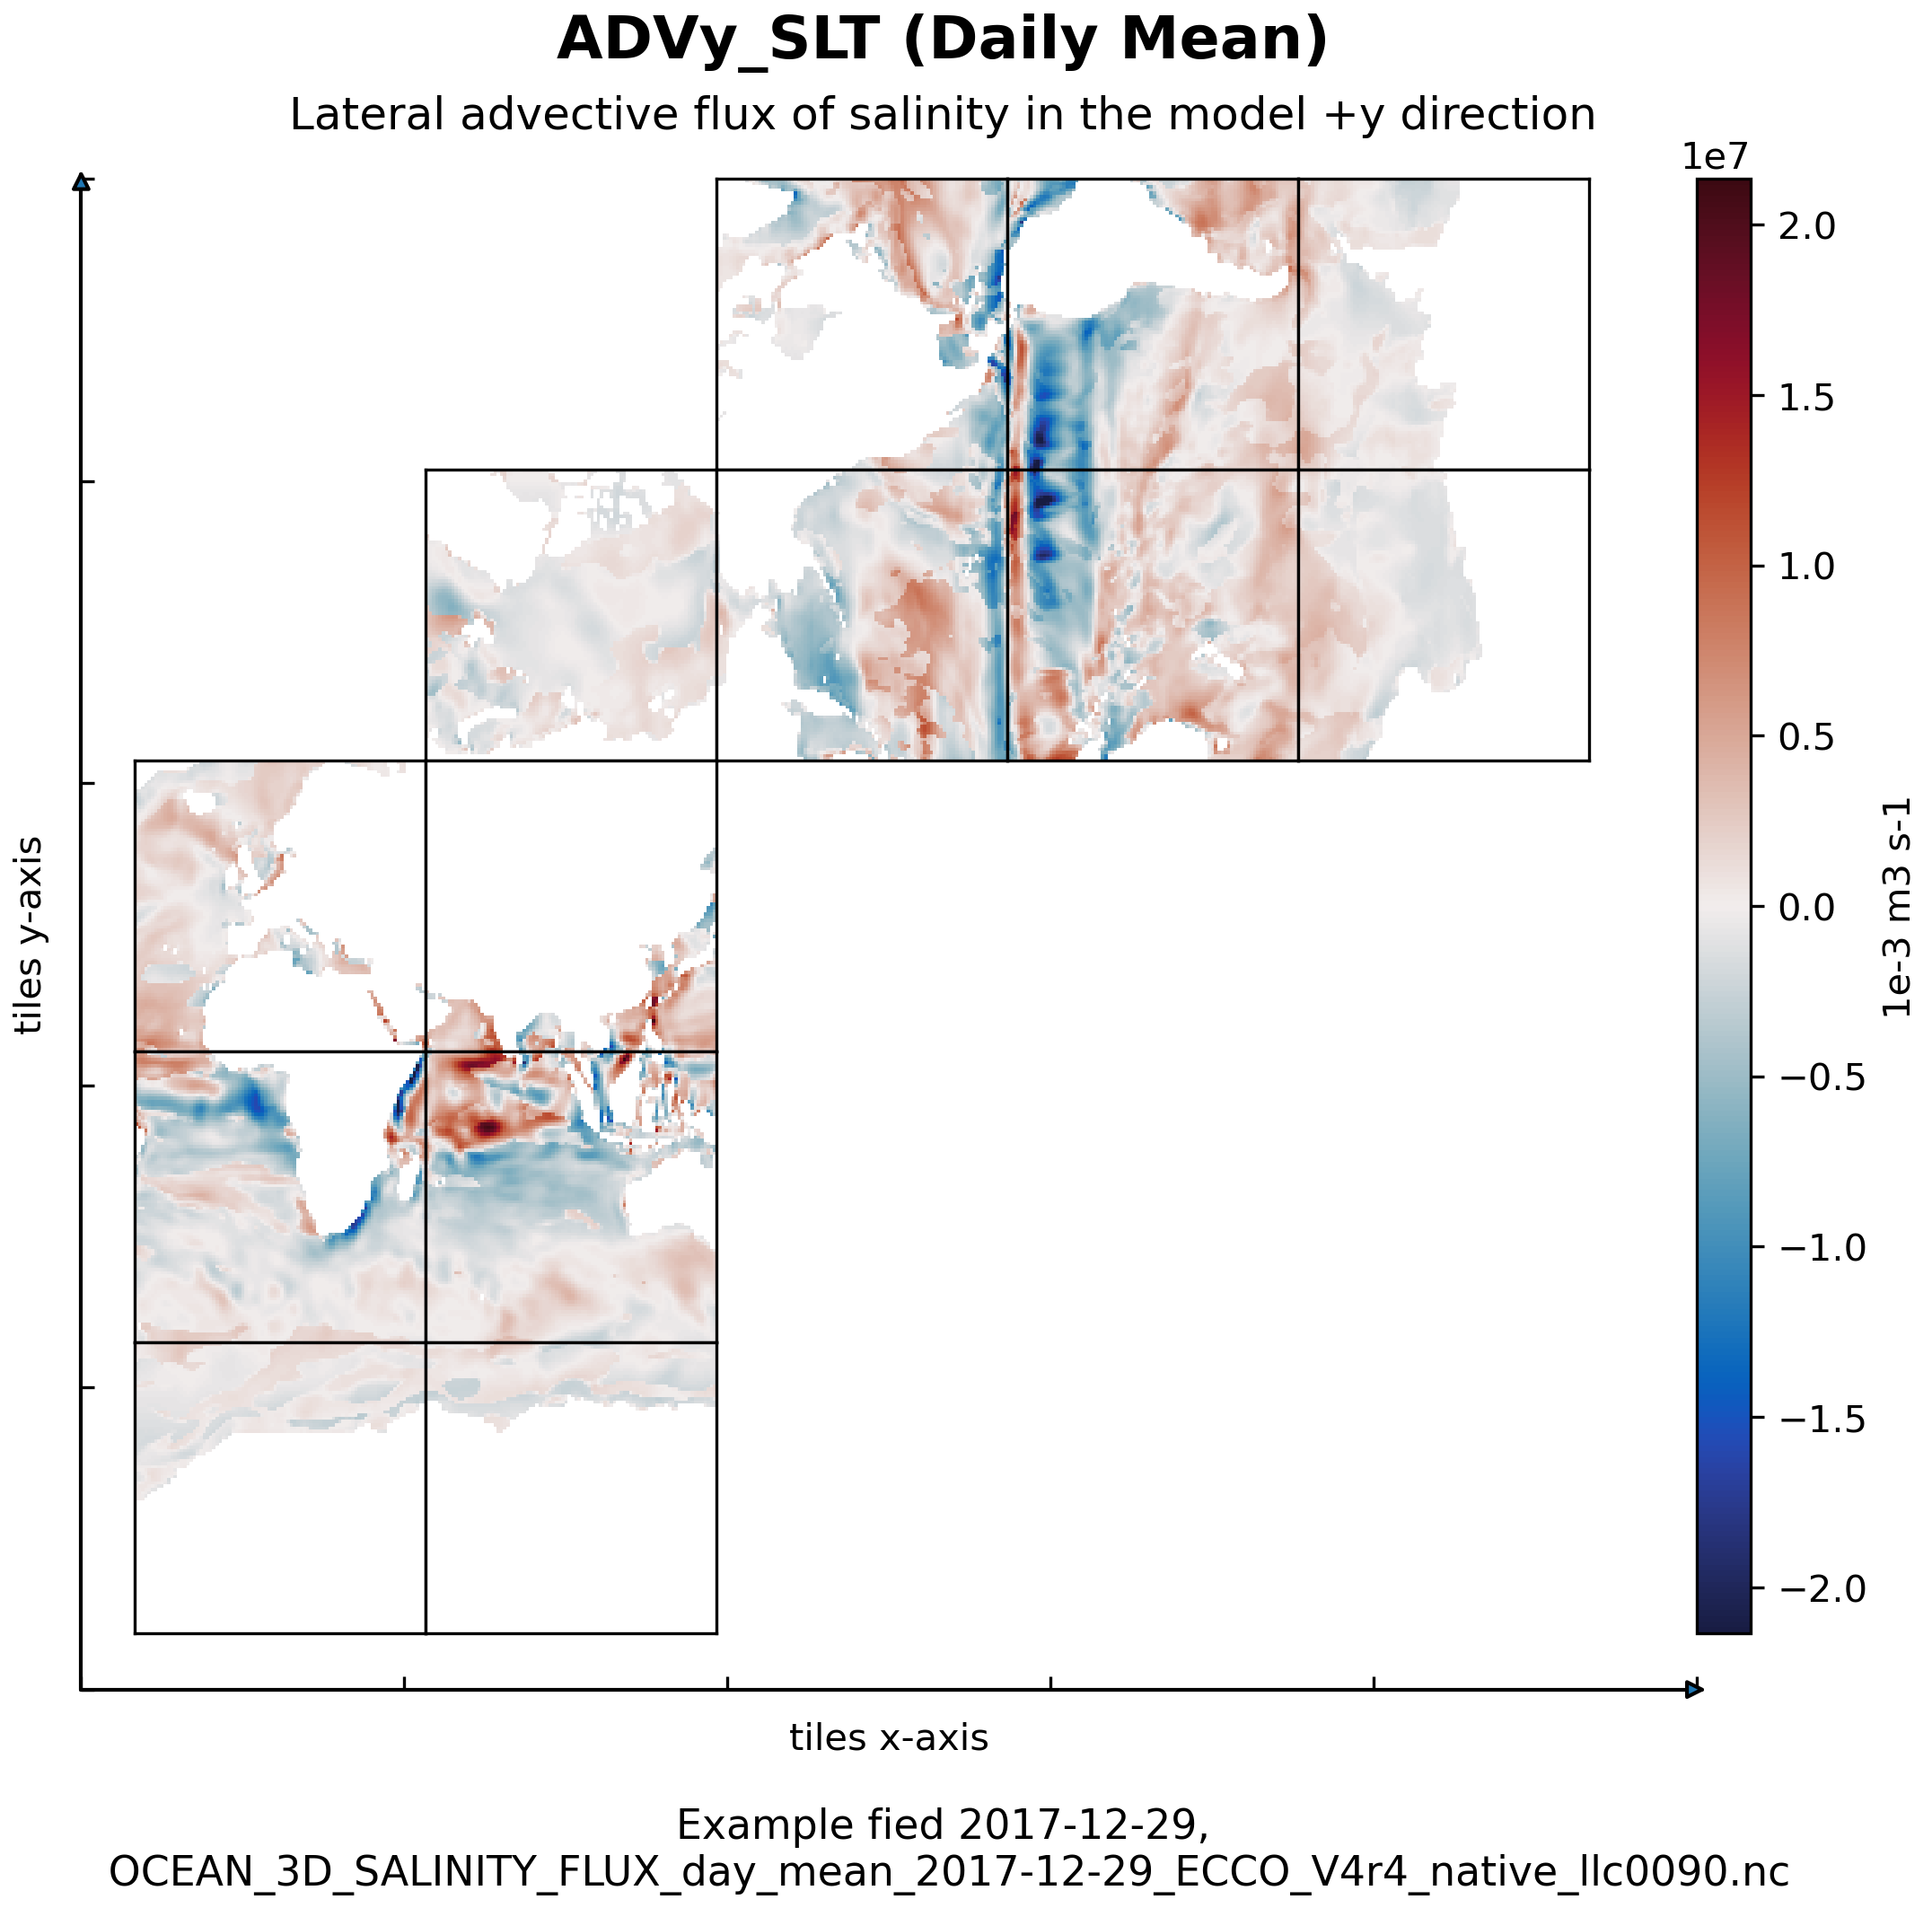
\includegraphics[scale=0.5]{../images/plots/native_plots/Ocean_Three-Dimensional_Salinity_Fluxes/ADVy_SLT.png}
\caption{\\Dataset: OCEAN\_3D\_SALINITY\_FLUX\\Variable: ADVy\_SLT}
\label{tab:table-OCEAN_3D_SALINITY_FLUX_ADVy_SLT-Plot}
\end{figure}
\pagebreak
\subsubsection{Native Variable DFrE\_SLT}
\begin{longtable}{|p{0.06\textwidth}|p{0.41\textwidth}|p{0.39\textwidth}|p{0.06\textwidth}|}
\caption{CDL description of OCEAN\_3D\_SALINITY\_FLUX's DFrE\_SLT variable}
\label{tab:table-OCEAN_3D_SALINITY_FLUX_DFrE_SLT} \\ 
\hline \endhead \hline \endfoot
\rowcolor{lightgray} \textbf{Storage Type} & \textbf{Variable Name} & \textbf{Description} & \textbf{Unit} \\ \hline
float32 & DFrE\_SLT & Vertical diffusive flux of salinity (explicit term) & 1e-3 m3 s-1 \\ \hline
\rowcolor{lightgray}  \multicolumn{4}{|p{1.00\textwidth}|}{\textbf{CDL Description}} \\ \hline
\multicolumn{4}{|p{1.00\textwidth}|}{\makecell{\parbox{1\textwidth}{float32 DFrE\_SLT(time, k\_l, tile, j, i)\\
\hspace*{0.5cm}DFrE\_SLT: \_FillValue = 9.96921e+36\\
\hspace*{0.5cm}DFrE\_SLT: long\_name = Vertical diffusive flux of salinity (explicit term)\\
\hspace*{0.5cm}DFrE\_SLT: units = 1e: 3 m3 s: 1\\
\hspace*{0.5cm}DFrE\_SLT: coverage\_content\_type = modelResult\\
\hspace*{0.5cm}DFrE\_SLT: direction = >0 decreases salinity (SALT)\\
\hspace*{0.5cm}DFrE\_SLT: coordinates = XC Zl YC time\\
\hspace*{0.5cm}DFrE\_SLT: valid\_min = : 1074719.375\\
\hspace*{0.5cm}DFrE\_SLT: valid\_max = 471215.75}}} \\ \hline
\rowcolor{lightgray} \multicolumn{4}{|p{1.00\textwidth}|}{\textbf{Comments}} \\ \hline
\multicolumn{4}{|p{1\textwidth}|}{The explicit term of the vertical diffusive flux of salinity (SALT) in the +z direction through the top 'w' face of the tracer cell on the native model grid. In the ECCO V4r4 model, an implicit scheme is used to calculate vertical diffusive tracer fluxes due to background diffusivity and the Kwz component of the GM-Redi tensor (vertical flux as a function of vertical gradient) while an explicit scheme is used to calculate the vertical diffusive fluxes from the Kwx and Kwy components of the GM-Redi tensor (vertical flux as a function of horizontal gradient). Both implicit and explicit components of vertical diffusive flux of salinity are provided. Note: in the Arakawa-C grid, vertical flux quantities are staggered relative to the tracer cells with indexing such that +DFrE\_SLT(i,j,k\_l) corresponds to upward +z fluxes through the top 'w' face of the tracer cell at (i,j,k). Salinity defined using CF convention 'Sea water salinity is the salt content of sea water, often on the Practical Salinity Scale of 1978. However, the unqualified term 'salinity' is generic and does not necessarily imply any particular method of calculation. The units of salinity are dimensionless and the units attribute should normally be given as 1e-3 or 0.001 i.e. parts per thousand.' see https://cfconventions.org/Data/cf-standard-names/73/build/cf-standard-name-table.html} \\ \hline
\end{longtable}

\begin{figure}[H]
\centering
\includegraphics[scale=0.5]{../images/plots/native_plots/Ocean_Three-Dimensional_Salinity_Fluxes/DFrE_SLT.png}
\caption{\\Dataset: OCEAN\_3D\_SALINITY\_FLUX\\Variable: DFrE\_SLT}
\label{tab:table-OCEAN_3D_SALINITY_FLUX_DFrE_SLT-Plot}
\end{figure}
\pagebreak
\subsubsection{Native Variable DFrI\_SLT}
\begin{longtable}{|p{0.06\textwidth}|p{0.41\textwidth}|p{0.39\textwidth}|p{0.06\textwidth}|}
\caption{CDL description of OCEAN\_3D\_SALINITY\_FLUX's DFrI\_SLT variable}
\label{tab:table-OCEAN_3D_SALINITY_FLUX_DFrI_SLT} \\ 
\hline \endhead \hline \endfoot
\rowcolor{lightgray} \textbf{Storage Type} & \textbf{Variable Name} & \textbf{Description} & \textbf{Unit} \\ \hline
float32 & DFrI\_SLT & Vertical diffusive flux of salinity (implicit term) & 1e-3 m3 s-1 \\ \hline
\rowcolor{lightgray}  \multicolumn{4}{|p{1.00\textwidth}|}{\textbf{CDL Description}} \\ \hline
\multicolumn{4}{|p{1.00\textwidth}|}{\makecell{\parbox{1\textwidth}{float32 DFrI\_SLT(time, k\_l, tile, j, i)\\
\hspace*{0.5cm}DFrI\_SLT: \_FillValue = 9.96921e+36\\
\hspace*{0.5cm}DFrI\_SLT: long\_name = Vertical diffusive flux of salinity (implicit term)\\
\hspace*{0.5cm}DFrI\_SLT: units = 1e: 3 m3 s: 1\\
\hspace*{0.5cm}DFrI\_SLT: coverage\_content\_type = modelResult\\
\hspace*{0.5cm}DFrI\_SLT: direction = >0 decreases salinity (SALT)\\
\hspace*{0.5cm}DFrI\_SLT: coordinates = XC Zl YC time\\
\hspace*{0.5cm}DFrI\_SLT: valid\_min = : 30609048.0\\
\hspace*{0.5cm}DFrI\_SLT: valid\_max = 3197643.0}}} \\ \hline
\rowcolor{lightgray} \multicolumn{4}{|p{1.00\textwidth}|}{\textbf{Comments}} \\ \hline
\multicolumn{4}{|p{1\textwidth}|}{The implicit term of the vertical diffusive flux of salinity (SALT) in the +z direction through the top 'w' face of the tracer cell on the native model grid. In the ECCO V4r4 model, an implicit scheme is used to calculate vertical diffusive tracer fluxes due to background diffusivity and the Kwz component of the GM-Redi tensor (vertical flux as a function of vertical gradient) while an explicit scheme is used to calculate the vertical diffusive fluxes from the Kwx and Kwy components of the GM-Redi tensor (vertical flux as a function of horizontal gradient). Both implicit and explicit components of vertical diffusive flux of salinity are provided. Note: in the Arakawa-C grid, vertical flux quantities are staggered relative to the tracer cells with indexing such that +DFrI\_SLT(i,j,k\_l) corresponds to upward +z fluxes through the top face 'w' of the tracer cell at (i,j,k). Salinity defined using CF convention 'Sea water salinity is the salt content of sea water, often on the Practical Salinity Scale of 1978. However, the unqualified term 'salinity' is generic and does not necessarily imply any particular method of calculation. The units of salinity are dimensionless and the units attribute should normally be given as 1e-3 or 0.001 i.e. parts per thousand.' see https://cfconventions.org/Data/cf-standard-names/73/build/cf-standard-name-table.html} \\ \hline
\end{longtable}

\begin{figure}[H]
\centering
\includegraphics[scale=0.5]{../images/plots/native_plots/Ocean_Three-Dimensional_Salinity_Fluxes/DFrI_SLT.png}
\caption{\\Dataset: OCEAN\_3D\_SALINITY\_FLUX\\Variable: DFrI\_SLT}
\label{tab:table-OCEAN_3D_SALINITY_FLUX_DFrI_SLT-Plot}
\end{figure}
\pagebreak
\subsubsection{Native Variable DFxE\_SLT}
\begin{longtable}{|p{0.06\textwidth}|p{0.41\textwidth}|p{0.39\textwidth}|p{0.06\textwidth}|}
\caption{CDL description of OCEAN\_3D\_SALINITY\_FLUX's DFxE\_SLT variable}
\label{tab:table-OCEAN_3D_SALINITY_FLUX_DFxE_SLT} \\ 
\hline \endhead \hline \endfoot
\rowcolor{lightgray} \textbf{Storage Type} & \textbf{Variable Name} & \textbf{Description} & \textbf{Unit} \\ \hline
float32 & DFxE\_SLT & Lateral diffusive flux of salinity in the model +x direction & 1e-3 m3 s-1 \\ \hline
\rowcolor{lightgray}  \multicolumn{4}{|p{1.00\textwidth}|}{\textbf{CDL Description}} \\ \hline
\multicolumn{4}{|p{1.00\textwidth}|}{\makecell{\parbox{1\textwidth}{float32 DFxE\_SLT(time, k, tile, j, i\_g)\\
\hspace*{0.5cm}DFxE\_SLT: \_FillValue = 9.96921e+36\\
\hspace*{0.5cm}DFxE\_SLT: long\_name = Lateral diffusive flux of salinity in the model +x direction\\
\hspace*{0.5cm}DFxE\_SLT: units = 1e: 3 m3 s: 1\\
\hspace*{0.5cm}DFxE\_SLT: mate = DFyE\_SLT\\
\hspace*{0.5cm}DFxE\_SLT: coverage\_content\_type = modelResult\\
\hspace*{0.5cm}DFxE\_SLT: direction = >0 increases salinity (SALT)\\
\hspace*{0.5cm}DFxE\_SLT: coordinates = Z time\\
\hspace*{0.5cm}DFxE\_SLT: valid\_min = : 125908.03125\\
\hspace*{0.5cm}DFxE\_SLT: valid\_max = 192716.484375}}} \\ \hline
\rowcolor{lightgray} \multicolumn{4}{|p{1.00\textwidth}|}{\textbf{Comments}} \\ \hline
\multicolumn{4}{|p{1\textwidth}|}{Lateral diffusive flux of salinity (SALT) in the +x direction through the 'u' face of the tracer cell on the native model grid. Note: in the Arakawa-C grid, horizontal flux quantities are staggered relative to the tracer cells with indexing such that +DFxE\_SLT(i\_g,j,k) corresponds to +x fluxes through the 'u' face of the tracer cell at (i,j,k). Also, the model +x direction does not necessarily correspond to the geographical east-west direction because the x and y axes of the model's curvilinear lat-lon-cap (llc) grid have arbitrary orientations which vary within and across tiles. Salinity defined using CF convention 'Sea water salinity is the salt content of sea water, often on the Practical Salinity Scale of 1978. However, the unqualified term 'salinity' is generic and does not necessarily imply any particular method of calculation. The units of salinity are dimensionless and the units attribute should normally be given as 1e-3 or 0.001 i.e. parts per thousand.' see https://cfconventions.org/Data/cf-standard-names/73/build/cf-standard-name-table.html} \\ \hline
\end{longtable}

\begin{figure}[H]
\centering
\includegraphics[scale=0.5]{../images/plots/native_plots/Ocean_Three-Dimensional_Salinity_Fluxes/DFxE_SLT.png}
\caption{\\Dataset: OCEAN\_3D\_SALINITY\_FLUX\\Variable: DFxE\_SLT}
\label{tab:table-OCEAN_3D_SALINITY_FLUX_DFxE_SLT-Plot}
\end{figure}
\pagebreak
\subsubsection{Native Variable DFyE\_SLT}
\begin{longtable}{|p{0.06\textwidth}|p{0.41\textwidth}|p{0.39\textwidth}|p{0.06\textwidth}|}
\caption{CDL description of OCEAN\_3D\_SALINITY\_FLUX's DFyE\_SLT variable}
\label{tab:table-OCEAN_3D_SALINITY_FLUX_DFyE_SLT} \\ 
\hline \endhead \hline \endfoot
\rowcolor{lightgray} \textbf{Storage Type} & \textbf{Variable Name} & \textbf{Description} & \textbf{Unit} \\ \hline
float32 & DFyE\_SLT & Lateral diffusive flux of salinity in the model +y direction & 1e-3 m3 s-1 \\ \hline
\rowcolor{lightgray}  \multicolumn{4}{|p{1.00\textwidth}|}{\textbf{CDL Description}} \\ \hline
\multicolumn{4}{|p{1.00\textwidth}|}{\makecell{\parbox{1\textwidth}{float32 DFyE\_SLT(time, k, tile, j\_g, i)\\
\hspace*{0.5cm}DFyE\_SLT: \_FillValue = 9.96921e+36\\
\hspace*{0.5cm}DFyE\_SLT: long\_name = Lateral diffusive flux of salinity in the model +y direction\\
\hspace*{0.5cm}DFyE\_SLT: units = 1e: 3 m3 s: 1\\
\hspace*{0.5cm}DFyE\_SLT: mate = DFxE\_SLT\\
\hspace*{0.5cm}DFyE\_SLT: coverage\_content\_type = modelResult\\
\hspace*{0.5cm}DFyE\_SLT: direction = >0 increases salinity (SALT)\\
\hspace*{0.5cm}DFyE\_SLT: coordinates = Z time\\
\hspace*{0.5cm}DFyE\_SLT: valid\_min = : 114959.2109375\\
\hspace*{0.5cm}DFyE\_SLT: valid\_max = 154227.140625}}} \\ \hline
\rowcolor{lightgray} \multicolumn{4}{|p{1.00\textwidth}|}{\textbf{Comments}} \\ \hline
\multicolumn{4}{|p{1\textwidth}|}{Lateral diffusive flux of salinity (SALT) in the +y direction through the 'v' face of the tracer cell on the native model grid. Note: in the Arakawa-C grid, horizontal flux quantities are staggered relative to the tracer cells with indexing such that +DFyE\_SLT(i,j\_g,k) corresponds to +y fluxes through the 'v' face of the tracer cell at (i,j,k). Also, the model +y direction does not necessarily correspond to the geographical north-south direction because the x and y axes of the model's curvilinear lat-lon-cap (llc) grid have arbitrary orientations which vary within and across tiles. Salinity defined using CF convention 'Sea water salinity is the salt content of sea water, often on the Practical Salinity Scale of 1978. However, the unqualified term 'salinity' is generic and does not necessarily imply any particular method of calculation. The units of salinity are dimensionless and the units attribute should normally be given as 1e-3 or 0.001 i.e. parts per thousand.' see https://cfconventions.org/Data/cf-standard-names/73/build/cf-standard-name-table.html} \\ \hline
\end{longtable}

\begin{figure}[H]
\centering
\includegraphics[scale=0.5]{../images/plots/native_plots/Ocean_Three-Dimensional_Salinity_Fluxes/DFyE_SLT.png}
\caption{\\Dataset: OCEAN\_3D\_SALINITY\_FLUX\\Variable: DFyE\_SLT}
\label{tab:table-OCEAN_3D_SALINITY_FLUX_DFyE_SLT-Plot}
\end{figure}
\pagebreak
\subsubsection{Native Variable oceSPtnd}
\begin{longtable}{|p{0.06\textwidth}|p{0.41\textwidth}|p{0.39\textwidth}|p{0.06\textwidth}|}
\caption{CDL description of OCEAN\_3D\_SALINITY\_FLUX's oceSPtnd variable}
\label{tab:table-OCEAN_3D_SALINITY_FLUX_oceSPtnd} \\ 
\hline \endhead \hline \endfoot
\rowcolor{lightgray} \textbf{Storage Type} & \textbf{Variable Name} & \textbf{Description} & \textbf{Unit} \\ \hline
float32 & oceSPtnd & Salt tendency due to the vertical transport of salt in high-salinity brine plumes & g m-2 s-1 \\ \hline
\rowcolor{lightgray}  \multicolumn{4}{|p{1.00\textwidth}|}{\textbf{CDL Description}} \\ \hline
\multicolumn{4}{|p{1.00\textwidth}|}{\makecell{\parbox{1\textwidth}{float32 oceSPtnd(time, k, tile, j, i)\\
\hspace*{0.5cm}oceSPtnd: \_FillValue = 9.96921e+36\\
\hspace*{0.5cm}oceSPtnd: long\_name = Salt tendency due to the vertical transport of salt in high: salinity brine plumes\\
\hspace*{0.5cm}oceSPtnd: units = g m: 2 s: 1\\
\hspace*{0.5cm}oceSPtnd: coverage\_content\_type = modelResult\\
\hspace*{0.5cm}oceSPtnd: direction = >0 increases salinity (SALT)\\
\hspace*{0.5cm}oceSPtnd: coordinates = XC Z YC time\\
\hspace*{0.5cm}oceSPtnd: valid\_min = 0.0\\
\hspace*{0.5cm}oceSPtnd: valid\_max = 0.021119138225913048}}} \\ \hline
\rowcolor{lightgray} \multicolumn{4}{|p{1.00\textwidth}|}{\textbf{Comments}} \\ \hline
\multicolumn{4}{|p{1\textwidth}|}{Salt tendency due to the vertical transport of salt in high-salinity brine plumes. Note: units are grams of salt per square meter per second, not salinity per square meter per second.} \\ \hline
\end{longtable}

\begin{figure}[H]
\centering
\includegraphics[scale=0.5]{../images/plots/native_plots/Ocean_Three-Dimensional_Salinity_Fluxes/oceSPtnd.png}
\caption{\\Dataset: OCEAN\_3D\_SALINITY\_FLUX\\Variable: oceSPtnd}
\label{tab:table-OCEAN_3D_SALINITY_FLUX_oceSPtnd-Plot}
\end{figure}
\pagebreak
\subsection{Native NetCDF OCEAN\_3D\_TEMPERATURE\_FLUX}
\newp
\begin{longtable}{|p{0.1\textwidth}|p{0.5\textwidth}|}
\caption{Variables in the dataset OCEAN\_3D\_TEMPERATURE\_FLUX}
\label{tab:table-OCEAN_3D_TEMPERATURE_FLUX-fields} \\ 
\hline \endhead \hline \endfoot
\rowcolor{lightgray} \textbf{Dataset:} & \textbf{OCEAN\_3D\_TEMPERATURE\_FLUX} \\ \hline
Field: &ADVx\_TH \\ \hline
Field: &DFxE\_TH \\ \hline
Field: &ADVy\_TH \\ \hline
Field: &DFyE\_TH \\ \hline
Field: &ADVr\_TH \\ \hline
Field: &DFrE\_TH \\ \hline
Field: &DFrI\_TH \\ \hline
\end{longtable}

\pagebreak
\subsubsection{Native Variable ADVr\_TH}
\begin{longtable}{|p{0.06\textwidth}|p{0.41\textwidth}|p{0.39\textwidth}|p{0.06\textwidth}|}
\caption{CDL description of OCEAN\_3D\_TEMPERATURE\_FLUX's ADVr\_TH variable}
\label{tab:table-OCEAN_3D_TEMPERATURE_FLUX_ADVr_TH} \\ 
\hline \endhead \hline \endfoot
\rowcolor{lightgray} \textbf{Storage Type} & \textbf{Variable Name} & \textbf{Description} & \textbf{Unit} \\ \hline
float32 & ADVr\_TH & Vertical advective flux of potential temperature & degree\_C m3 s-1 \\ \hline
\rowcolor{lightgray}  \multicolumn{4}{|p{1.00\textwidth}|}{\textbf{CDL Description}} \\ \hline
\multicolumn{4}{|p{1.00\textwidth}|}{\makecell{\parbox{1\textwidth}{float32 ADVr\_TH(time, k\_l, tile, j, i)\\
\hspace*{0.5cm}ADVr\_TH: \_FillValue = 9.96921e+36\\
\hspace*{0.5cm}ADVr\_TH: long\_name = Vertical advective flux of potential temperature\\
\hspace*{0.5cm}ADVr\_TH: units = degree\_C m3 s: 1\\
\hspace*{0.5cm}ADVr\_TH: coverage\_content\_type = modelResult\\
\hspace*{0.5cm}ADVr\_TH: direction = >0 decreases potential temperature (THETA)\\
\hspace*{0.5cm}ADVr\_TH: coordinates = XC YC time Zl\\
\hspace*{0.5cm}ADVr\_TH: valid\_min = : 125094904.0\\
\hspace*{0.5cm}ADVr\_TH: valid\_max = 179459344.0}}} \\ \hline
\rowcolor{lightgray} \multicolumn{4}{|p{1.00\textwidth}|}{\textbf{Comments}} \\ \hline
\multicolumn{4}{|p{1\textwidth}|}{Vertical advective flux of potential temperature (THETA) in the +z direction through the top 'w' face of the tracer cell on the native model grid. Note: in the Arakawa-C grid, vertical flux quantities are staggered relative to the tracer cells with indexing such that +ADVr\_TH(i,j,k\_l) corresponds to upward +z fluxes through the top 'w' face of the tracer cell at (i,j,k)} \\ \hline
\end{longtable}

\begin{figure}[H]
\centering
\includegraphics[scale=0.5]{../images/plots/native_plots/Ocean_Three-Dimensional_Potential_Temperature_Fluxes/ADVr_TH.png}
\caption{\\Dataset: OCEAN\_3D\_TEMPERATURE\_FLUX\\Variable: ADVr\_TH}
\label{tab:table-OCEAN_3D_TEMPERATURE_FLUX_ADVr_TH-Plot}
\end{figure}
\pagebreak
\subsubsection{Native Variable ADVx\_TH}
\begin{longtable}{|p{0.06\textwidth}|p{0.41\textwidth}|p{0.39\textwidth}|p{0.06\textwidth}|}
\caption{CDL description of OCEAN\_3D\_TEMPERATURE\_FLUX's ADVx\_TH variable}
\label{tab:table-OCEAN_3D_TEMPERATURE_FLUX_ADVx_TH} \\ 
\hline \endhead \hline \endfoot
\rowcolor{lightgray} \textbf{Storage Type} & \textbf{Variable Name} & \textbf{Description} & \textbf{Unit} \\ \hline
float32 & ADVx\_TH & Lateral advective flux of potential temperature in the model +x direction & degree\_C m3 s-1 \\ \hline
\rowcolor{lightgray}  \multicolumn{4}{|p{1.00\textwidth}|}{\textbf{CDL Description}} \\ \hline
\multicolumn{4}{|p{1.00\textwidth}|}{\makecell{\parbox{1\textwidth}{float32 ADVx\_TH(time, k, tile, j, i\_g)\\
\hspace*{0.5cm}ADVx\_TH: \_FillValue = 9.96921e+36\\
\hspace*{0.5cm}ADVx\_TH: long\_name = Lateral advective flux of potential temperature in the model +x direction\\
\hspace*{0.5cm}ADVx\_TH: units = degree\_C m3 s: 1\\
\hspace*{0.5cm}ADVx\_TH: mate = ADVy\_TH\\
\hspace*{0.5cm}ADVx\_TH: coverage\_content\_type = modelResult\\
\hspace*{0.5cm}ADVx\_TH: direction = >0 increases potential temperature (THETA)\\
\hspace*{0.5cm}ADVx\_TH: coordinates = time Z\\
\hspace*{0.5cm}ADVx\_TH: valid\_min = : 38210700.0\\
\hspace*{0.5cm}ADVx\_TH: valid\_max = 38049636.0}}} \\ \hline
\rowcolor{lightgray} \multicolumn{4}{|p{1.00\textwidth}|}{\textbf{Comments}} \\ \hline
\multicolumn{4}{|p{1\textwidth}|}{Lateral advective flux of potential temperature (THETA) in the +x direction through the 'u' face of the tracer cell on the native model grid. Note: in the Arakawa-C grid, horizontal flux quantities are staggered relative to the tracer cells with indexing such that +ADVx\_TH(i\_g,j,k) corresponds to +x fluxes through the 'u' face of the tracer cell at (i,j,k). Also, the model +x direction does not necessarily correspond to the geographical east-west direction because the x and y axes of the model's lat-lon-cap (llc) curvilinear lat-lon-cap (llc) grid have arbitrary orientations which vary within and across tiles.} \\ \hline
\end{longtable}

\begin{figure}[H]
\centering
\includegraphics[scale=0.5]{../images/plots/native_plots/Ocean_Three-Dimensional_Potential_Temperature_Fluxes/ADVx_TH.png}
\caption{\\Dataset: OCEAN\_3D\_TEMPERATURE\_FLUX\\Variable: ADVx\_TH}
\label{tab:table-OCEAN_3D_TEMPERATURE_FLUX_ADVx_TH-Plot}
\end{figure}
\pagebreak
\subsubsection{Native Variable ADVy\_TH}
\begin{longtable}{|p{0.06\textwidth}|p{0.41\textwidth}|p{0.39\textwidth}|p{0.06\textwidth}|}
\caption{CDL description of OCEAN\_3D\_TEMPERATURE\_FLUX's ADVy\_TH variable}
\label{tab:table-OCEAN_3D_TEMPERATURE_FLUX_ADVy_TH} \\ 
\hline \endhead \hline \endfoot
\rowcolor{lightgray} \textbf{Storage Type} & \textbf{Variable Name} & \textbf{Description} & \textbf{Unit} \\ \hline
float32 & ADVy\_TH & Lateral advective flux of potential temperature in the model +y direction & degree\_C m3 s-1 \\ \hline
\rowcolor{lightgray}  \multicolumn{4}{|p{1.00\textwidth}|}{\textbf{CDL Description}} \\ \hline
\multicolumn{4}{|p{1.00\textwidth}|}{\makecell{\parbox{1\textwidth}{float32 ADVy\_TH(time, k, tile, j\_g, i)\\
\hspace*{0.5cm}ADVy\_TH: \_FillValue = 9.96921e+36\\
\hspace*{0.5cm}ADVy\_TH: long\_name = Lateral advective flux of potential temperature in the model +y direction\\
\hspace*{0.5cm}ADVy\_TH: units = degree\_C m3 s: 1\\
\hspace*{0.5cm}ADVy\_TH: mate = ADVx\_TH\\
\hspace*{0.5cm}ADVy\_TH: coverage\_content\_type = modelResult\\
\hspace*{0.5cm}ADVy\_TH: direction = >0 increases potential temperature (THETA)\\
\hspace*{0.5cm}ADVy\_TH: coordinates = time Z\\
\hspace*{0.5cm}ADVy\_TH: valid\_min = : 43909120.0\\
\hspace*{0.5cm}ADVy\_TH: valid\_max = 56347884.0}}} \\ \hline
\rowcolor{lightgray} \multicolumn{4}{|p{1.00\textwidth}|}{\textbf{Comments}} \\ \hline
\multicolumn{4}{|p{1\textwidth}|}{Lateral advective flux of potential temperature (THETA) in the +y direction through the 'v' face of the tracer cell on the native model grid. Note: in the Arakawa-C grid, horizontal flux quantities are staggered relative to the tracer cells with indexing such that +ADVy\_TH(i,j\_g,k) corresponds to +y fluxes through the 'v' face of the tracer cell at (i,j,k). Also, the model +y direction does not necessarily correspond to the geographical north-south direction because the x and y axes of the model's curvilinear lat-lon-cap (llc) grid have arbitrary orientations which vary within and across tiles.} \\ \hline
\end{longtable}

\begin{figure}[H]
\centering
\includegraphics[scale=0.5]{../images/plots/native_plots/Ocean_Three-Dimensional_Potential_Temperature_Fluxes/ADVy_TH.png}
\caption{\\Dataset: OCEAN\_3D\_TEMPERATURE\_FLUX\\Variable: ADVy\_TH}
\label{tab:table-OCEAN_3D_TEMPERATURE_FLUX_ADVy_TH-Plot}
\end{figure}
\pagebreak
\subsubsection{Native Variable DFrE\_TH}
\begin{longtable}{|p{0.06\textwidth}|p{0.41\textwidth}|p{0.39\textwidth}|p{0.06\textwidth}|}
\caption{CDL description of OCEAN\_3D\_TEMPERATURE\_FLUX's DFrE\_TH variable}
\label{tab:table-OCEAN_3D_TEMPERATURE_FLUX_DFrE_TH} \\ 
\hline \endhead \hline \endfoot
\rowcolor{lightgray} \textbf{Storage Type} & \textbf{Variable Name} & \textbf{Description} & \textbf{Unit} \\ \hline
float32 & DFrE\_TH & Vertical diffusive flux of potential temperature (explicit term) & degree\_C m3 s-1 \\ \hline
\rowcolor{lightgray}  \multicolumn{4}{|p{1.00\textwidth}|}{\textbf{CDL Description}} \\ \hline
\multicolumn{4}{|p{1.00\textwidth}|}{\makecell{\parbox{1\textwidth}{float32 DFrE\_TH(time, k\_l, tile, j, i)\\
\hspace*{0.5cm}DFrE\_TH: \_FillValue = 9.96921e+36\\
\hspace*{0.5cm}DFrE\_TH: long\_name = Vertical diffusive flux of potential temperature (explicit term)\\
\hspace*{0.5cm}DFrE\_TH: units = degree\_C m3 s: 1\\
\hspace*{0.5cm}DFrE\_TH: coverage\_content\_type = modelResult\\
\hspace*{0.5cm}DFrE\_TH: direction = >0 decreases potential temperature (THETA)\\
\hspace*{0.5cm}DFrE\_TH: coordinates = XC YC time Zl\\
\hspace*{0.5cm}DFrE\_TH: valid\_min = : 2632379.75\\
\hspace*{0.5cm}DFrE\_TH: valid\_max = 2659875.25}}} \\ \hline
\rowcolor{lightgray} \multicolumn{4}{|p{1.00\textwidth}|}{\textbf{Comments}} \\ \hline
\multicolumn{4}{|p{1\textwidth}|}{The explicit term of the vertical diffusive flux of potential temperature (THETA) in the +z direction through the top 'w' face of the tracer cell on the native model grid. In the ECCO V4r4 model, an implicit scheme is used to calculate vertical diffusive tracer fluxes due to background diffusivity and the Kwz component of the GM-Redi tensor (vertical flux as a function of vertical gradient) while an explicit scheme is used to calculate the vertical diffusive fluxes from the Kwx and Kwy components of the GM-Redi tensor (vertical flux as a function of horizontal gradient). Both implicit and explicit components of vertical diffusive flux of potential temperature are provided. Note: in the Arakawa-C grid, vertical flux quantities are staggered relative to the tracer cells with indexing such that +DFrE\_TH(i,j,k\_l) corresponds to upward +z fluxes through the top 'w' face of the tracer cell at (i,j,k).} \\ \hline
\end{longtable}

\begin{figure}[H]
\centering
\includegraphics[scale=0.5]{../images/plots/native_plots/Ocean_Three-Dimensional_Potential_Temperature_Fluxes/DFrE_TH.png}
\caption{\\Dataset: OCEAN\_3D\_TEMPERATURE\_FLUX\\Variable: DFrE\_TH}
\label{tab:table-OCEAN_3D_TEMPERATURE_FLUX_DFrE_TH-Plot}
\end{figure}
\pagebreak
\subsubsection{Native Variable DFrI\_TH}
\begin{longtable}{|p{0.06\textwidth}|p{0.41\textwidth}|p{0.39\textwidth}|p{0.06\textwidth}|}
\caption{CDL description of OCEAN\_3D\_TEMPERATURE\_FLUX's DFrI\_TH variable}
\label{tab:table-OCEAN_3D_TEMPERATURE_FLUX_DFrI_TH} \\ 
\hline \endhead \hline \endfoot
\rowcolor{lightgray} \textbf{Storage Type} & \textbf{Variable Name} & \textbf{Description} & \textbf{Unit} \\ \hline
float32 & DFrI\_TH & Vertical diffusive flux of potential temperature (implicit term) & degree\_C m3 s-1 \\ \hline
\rowcolor{lightgray}  \multicolumn{4}{|p{1.00\textwidth}|}{\textbf{CDL Description}} \\ \hline
\multicolumn{4}{|p{1.00\textwidth}|}{\makecell{\parbox{1\textwidth}{float32 DFrI\_TH(time, k\_l, tile, j, i)\\
\hspace*{0.5cm}DFrI\_TH: \_FillValue = 9.96921e+36\\
\hspace*{0.5cm}DFrI\_TH: long\_name = Vertical diffusive flux of potential temperature (implicit term)\\
\hspace*{0.5cm}DFrI\_TH: units = degree\_C m3 s: 1\\
\hspace*{0.5cm}DFrI\_TH: coverage\_content\_type = modelResult\\
\hspace*{0.5cm}DFrI\_TH: direction = >0 decreases potential temperature (THETA)\\
\hspace*{0.5cm}DFrI\_TH: coordinates = XC YC time Zl\\
\hspace*{0.5cm}DFrI\_TH: valid\_min = : 104210688.0\\
\hspace*{0.5cm}DFrI\_TH: valid\_max = 23574302.0}}} \\ \hline
\rowcolor{lightgray} \multicolumn{4}{|p{1.00\textwidth}|}{\textbf{Comments}} \\ \hline
\multicolumn{4}{|p{1\textwidth}|}{The implicit term of the vertical diffusive flux of potential temperature (THETA) in the +z direction through the top 'w' face of the tracer cell on the native model grid. In the ECCO V4r4 model, an implicit scheme is used to calculate vertical diffusive tracer fluxes due to background diffusivity and the Kwz component of the GM-Redi tensor (vertical flux as a function of vertical gradient) while an explicit scheme is used to calculate the vertical diffusive fluxes from the Kwx and Kwy components of the GM-Redi tensor (vertical flux as a function of horizontal gradient). Both implicit and explicit components of vertical diffusive flux of potential temperature are provided. Note: in the Arakawa-C grid, vertical flux quantities are staggered relative to the tracer cells with indexing such that +DFrI\_TH(i,j,k\_l) corresponds to upward +z fluxes through the top 'w' face of the tracer cell at (i,j,k)} \\ \hline
\end{longtable}

\begin{figure}[H]
\centering
\includegraphics[scale=0.5]{../images/plots/native_plots/Ocean_Three-Dimensional_Potential_Temperature_Fluxes/DFrI_TH.png}
\caption{\\Dataset: OCEAN\_3D\_TEMPERATURE\_FLUX\\Variable: DFrI\_TH}
\label{tab:table-OCEAN_3D_TEMPERATURE_FLUX_DFrI_TH-Plot}
\end{figure}
\pagebreak
\subsubsection{Native Variable DFxE\_TH}
\begin{longtable}{|p{0.06\textwidth}|p{0.41\textwidth}|p{0.39\textwidth}|p{0.06\textwidth}|}
\caption{CDL description of OCEAN\_3D\_TEMPERATURE\_FLUX's DFxE\_TH variable}
\label{tab:table-OCEAN_3D_TEMPERATURE_FLUX_DFxE_TH} \\ 
\hline \endhead \hline \endfoot
\rowcolor{lightgray} \textbf{Storage Type} & \textbf{Variable Name} & \textbf{Description} & \textbf{Unit} \\ \hline
float32 & DFxE\_TH & Lateral diffusive flux of potential temperature in the model +x direction & degree\_C m3 s-1 \\ \hline
\rowcolor{lightgray}  \multicolumn{4}{|p{1.00\textwidth}|}{\textbf{CDL Description}} \\ \hline
\multicolumn{4}{|p{1.00\textwidth}|}{\makecell{\parbox{1\textwidth}{float32 DFxE\_TH(time, k, tile, j, i\_g)\\
\hspace*{0.5cm}DFxE\_TH: \_FillValue = 9.96921e+36\\
\hspace*{0.5cm}DFxE\_TH: long\_name = Lateral diffusive flux of potential temperature in the model +x direction\\
\hspace*{0.5cm}DFxE\_TH: units = degree\_C m3 s: 1\\
\hspace*{0.5cm}DFxE\_TH: mate = DFyE\_TH\\
\hspace*{0.5cm}DFxE\_TH: coverage\_content\_type = modelResult\\
\hspace*{0.5cm}DFxE\_TH: direction = >0 increases potential temperature (THETA)\\
\hspace*{0.5cm}DFxE\_TH: coordinates = time Z\\
\hspace*{0.5cm}DFxE\_TH: valid\_min = : 582494.125\\
\hspace*{0.5cm}DFxE\_TH: valid\_max = 698695.75}}} \\ \hline
\rowcolor{lightgray} \multicolumn{4}{|p{1.00\textwidth}|}{\textbf{Comments}} \\ \hline
\multicolumn{4}{|p{1\textwidth}|}{Lateral diffusive flux of potential temperature (THETA) in the +x direction through the 'u' face of the tracer cell on the native model grid. Note: in the Arakawa-C grid, horizontal flux quantities are staggered relative to the tracer cells with indexing such that +DFxE\_TH(i\_g,j,k) corresponds to +x fluxes through the 'u' face of the tracer cell at (i,j,k). Also, the model +x direction does not necessarily correspond to the geographical east-west direction because the x and y axes of the model's curvilinear lat-lon-cap (llc) grid have arbitrary orientations which vary within and across tiles.} \\ \hline
\end{longtable}

\begin{figure}[H]
\centering
\includegraphics[scale=0.5]{../images/plots/native_plots/Ocean_Three-Dimensional_Potential_Temperature_Fluxes/DFxE_TH.png}
\caption{\\Dataset: OCEAN\_3D\_TEMPERATURE\_FLUX\\Variable: DFxE\_TH}
\label{tab:table-OCEAN_3D_TEMPERATURE_FLUX_DFxE_TH-Plot}
\end{figure}
\pagebreak
\subsubsection{Native Variable DFyE\_TH}
\begin{longtable}{|p{0.06\textwidth}|p{0.41\textwidth}|p{0.39\textwidth}|p{0.06\textwidth}|}
\caption{CDL description of OCEAN\_3D\_TEMPERATURE\_FLUX's DFyE\_TH variable}
\label{tab:table-OCEAN_3D_TEMPERATURE_FLUX_DFyE_TH} \\ 
\hline \endhead \hline \endfoot
\rowcolor{lightgray} \textbf{Storage Type} & \textbf{Variable Name} & \textbf{Description} & \textbf{Unit} \\ \hline
float32 & DFyE\_TH & Lateral diffusive flux of potential temperature in the model +y direction. & degree\_C m3 s-1 \\ \hline
\rowcolor{lightgray}  \multicolumn{4}{|p{1.00\textwidth}|}{\textbf{CDL Description}} \\ \hline
\multicolumn{4}{|p{1.00\textwidth}|}{\makecell{\parbox{1\textwidth}{float32 DFyE\_TH(time, k, tile, j\_g, i)\\
\hspace*{0.5cm}DFyE\_TH: \_FillValue = 9.96921e+36\\
\hspace*{0.5cm}DFyE\_TH: long\_name = Lateral diffusive flux of potential temperature in the model +y direction.\\
\hspace*{0.5cm}DFyE\_TH: units = degree\_C m3 s: 1\\
\hspace*{0.5cm}DFyE\_TH: mate = DFxE\_TH\\
\hspace*{0.5cm}DFyE\_TH: coverage\_content\_type = modelResult\\
\hspace*{0.5cm}DFyE\_TH: direction = >0 increases potential temperature (THETA)\\
\hspace*{0.5cm}DFyE\_TH: coordinates = time Z\\
\hspace*{0.5cm}DFyE\_TH: valid\_min = : 421044.78125\\
\hspace*{0.5cm}DFyE\_TH: valid\_max = 1053781.25}}} \\ \hline
\rowcolor{lightgray} \multicolumn{4}{|p{1.00\textwidth}|}{\textbf{Comments}} \\ \hline
\multicolumn{4}{|p{1\textwidth}|}{Lateral diffusive flux of potential temperature (THETA) in the +y direction through the 'v' face of the tracer cell on the native model grid. Note: in the Arakawa-C grid, horizontal flux quantities are staggered relative to the tracer cells with indexing such that +DFyE\_TH(i,j\_g,k) corresponds to +y fluxes through the 'v' face of the tracer cell at (i,j,k). Also, the model +y direction does not necessarily correspond to the geographical north-south direction because the x and y axes of the model's curvilinear lat-lon-cap (llc) grid have arbitrary orientations which vary within and across tiles.} \\ \hline
\end{longtable}

\begin{figure}[H]
\centering
\includegraphics[scale=0.5]{../images/plots/native_plots/Ocean_Three-Dimensional_Potential_Temperature_Fluxes/DFyE_TH.png}
\caption{\\Dataset: OCEAN\_3D\_TEMPERATURE\_FLUX\\Variable: DFyE\_TH}
\label{tab:table-OCEAN_3D_TEMPERATURE_FLUX_DFyE_TH-Plot}
\end{figure}
\pagebreak
\subsection{Native NetCDF OCEAN\_3D\_VOLUME\_FLUX}
\newp
\begin{longtable}{|p{0.1\textwidth}|p{0.5\textwidth}|}
\caption{Variables in the dataset OCEAN\_3D\_VOLUME\_FLUX}
\label{tab:table-OCEAN_3D_VOLUME_FLUX-fields} \\ 
\hline \endhead \hline \endfoot
\rowcolor{lightgray} \textbf{Dataset:} & \textbf{OCEAN\_3D\_VOLUME\_FLUX} \\ \hline
Field: &UVELMASS \\ \hline
Field: &VVELMASS \\ \hline
Field: &WVELMASS \\ \hline
\end{longtable}

\pagebreak
\subsubsection{Native Variable UVELMASS}
\begin{longtable}{|p{0.06\textwidth}|p{0.41\textwidth}|p{0.39\textwidth}|p{0.06\textwidth}|}
\caption{CDL description of OCEAN\_3D\_VOLUME\_FLUX's UVELMASS variable}
\label{tab:table-OCEAN_3D_VOLUME_FLUX_UVELMASS} \\ 
\hline \endhead \hline \endfoot
\rowcolor{lightgray} \textbf{Storage Type} & \textbf{Variable Name} & \textbf{Description} & \textbf{Unit} \\ \hline
float32 & UVELMASS & Horizontal velocity in the model +x direction per unit area of the grid cell 'u' face & m s-1 \\ \hline
\rowcolor{lightgray}  \multicolumn{4}{|p{1.00\textwidth}|}{\textbf{CDL Description}} \\ \hline
\multicolumn{4}{|p{1.00\textwidth}|}{\makecell{\parbox{1\textwidth}{float32 UVELMASS(time, k, tile, j, i\_g)\\
\hspace*{0.5cm}UVELMASS: \_FillValue = 9.96921e+36\\
\hspace*{0.5cm}UVELMASS: long\_name = "Horizontal velocity in the model +x direction per unit area of the grid cell u face"\\
\hspace*{0.5cm}UVELMASS: units = m s: 1\\
\hspace*{0.5cm}UVELMASS: mate = VVELMASS\\
\hspace*{0.5cm}UVELMASS: coverage\_content\_type = modelResult\\
\hspace*{0.5cm}UVELMASS: direction = >0 increases volume\\
\hspace*{0.5cm}UVELMASS: coordinates = Z time\\
\hspace*{0.5cm}UVELMASS: valid\_min = : 2.115365505218506\\
\hspace*{0.5cm}UVELMASS: valid\_max = 2.0377726554870605}}} \\ \hline
\rowcolor{lightgray} \multicolumn{4}{|p{1.00\textwidth}|}{\textbf{Comments}} \\ \hline
\multicolumn{4}{|p{1\textwidth}|}{Horizontal velocity in the model +x direction averaged over the area of the tracer grid cell 'u' face on the native model grid ('u' grid cell face area = drF dyG). Accounts for partial cells (hFacW < 1) and for time-varying grid cell thickness (z* coordinate system). Volume flux in +x = UVELMASS drF dyG. Note: in the Arakawa-C grid, horizontal velocities are staggered relative to the tracer cells with indexing such that +UVELMASS(i,j,k) corresponds to +x fluxes through the 'u' face of the tracer cell at (i,j,k). UVELMASS can be used for volume flux calculations because it accounts for the grid cell thicknesses variations in the +x direction (hFacW) with time (z* coordinate system). Also, the model +x direction does not necessarily correspond to the geographical east-west direction because the x and y axes of the model's curvilinear lat-lon-cap (llc) grid have arbitrary orientations which vary within and across tiles. See VVELMASS and WVELMASS} \\ \hline
\end{longtable}

\begin{figure}[H]
\centering
\includegraphics[scale=0.5]{../images/plots/native_plots/Ocean_Three-Dimensional_Volume_Fluxes/UVELMASS.png}
\caption{\\Dataset: OCEAN\_3D\_VOLUME\_FLUX\\Variable: UVELMASS}
\label{tab:table-OCEAN_3D_VOLUME_FLUX_UVELMASS-Plot}
\end{figure}
\pagebreak
\subsubsection{Native Variable VVELMASS}
\begin{longtable}{|p{0.06\textwidth}|p{0.41\textwidth}|p{0.39\textwidth}|p{0.06\textwidth}|}
\caption{CDL description of OCEAN\_3D\_VOLUME\_FLUX's VVELMASS variable}
\label{tab:table-OCEAN_3D_VOLUME_FLUX_VVELMASS} \\ 
\hline \endhead \hline \endfoot
\rowcolor{lightgray} \textbf{Storage Type} & \textbf{Variable Name} & \textbf{Description} & \textbf{Unit} \\ \hline
float32 & VVELMASS & Horizontal velocity in the model +y direction per unit area of the grid cell 'v' face & m s-1 m3 m-3 \\ \hline
\rowcolor{lightgray}  \multicolumn{4}{|p{1.00\textwidth}|}{\textbf{CDL Description}} \\ \hline
\multicolumn{4}{|p{1.00\textwidth}|}{\makecell{\parbox{1\textwidth}{float32 VVELMASS(time, k, tile, j\_g, i)\\
\hspace*{0.5cm}VVELMASS: \_FillValue = 9.96921e+36\\
\hspace*{0.5cm}VVELMASS: long\_name = "Horizontal velocity in the model +y direction per unit area of the grid cell v face"\\
\hspace*{0.5cm}VVELMASS: units = m s: 1 m3 m: 3\\
\hspace*{0.5cm}VVELMASS: mate = UVELMASS\\
\hspace*{0.5cm}VVELMASS: coverage\_content\_type = modelResult\\
\hspace*{0.5cm}VVELMASS: direction = >0 increases volume\\
\hspace*{0.5cm}VVELMASS: coordinates = Z time\\
\hspace*{0.5cm}VVELMASS: valid\_min = : 1.7897182703018188\\
\hspace*{0.5cm}VVELMASS: valid\_max = 1.9216758012771606}}} \\ \hline
\rowcolor{lightgray} \multicolumn{4}{|p{1.00\textwidth}|}{\textbf{Comments}} \\ \hline
\multicolumn{4}{|p{1\textwidth}|}{Horizontal velocity in the model +y direction averaged over the area of the tracer grid cell 'v' face on the native model grid ('v' grid cell face area = drF dxG). Accounts for partial cells (hFacS < 1) and for time-varying grid cell thickness (z* coordinate system). Volume flux in +y = VVELMASS drF dxG. Note: in the Arakawa-C grid, horizontal velocities are staggered relative to the tracer cells with indexing such that +VVELMASS(i,j,k) corresponds to +y fluxes through the 'v' face of the tracer cell at (i,j,k). VVELMASS can be used for volume flux calculations because it accounts for grid cell thicknesses variations in the +y direction (hFacS) with time (z* coordinate system). Also, the model +y direction does not necessarily correspond to the geographical north-south direction because the x and y axes of the model's curvilinear lat-lon-cap (llc) grid have arbitrary orientations which vary within and across tiles. See UVELMASS and WVELMASS.} \\ \hline
\end{longtable}

\begin{figure}[H]
\centering
\includegraphics[scale=0.5]{../images/plots/native_plots/Ocean_Three-Dimensional_Volume_Fluxes/VVELMASS.png}
\caption{\\Dataset: OCEAN\_3D\_VOLUME\_FLUX\\Variable: VVELMASS}
\label{tab:table-OCEAN_3D_VOLUME_FLUX_VVELMASS-Plot}
\end{figure}
\pagebreak
\subsubsection{Native Variable WVELMASS}
\begin{longtable}{|p{0.06\textwidth}|p{0.41\textwidth}|p{0.39\textwidth}|p{0.06\textwidth}|}
\caption{CDL description of OCEAN\_3D\_VOLUME\_FLUX's WVELMASS variable}
\label{tab:table-OCEAN_3D_VOLUME_FLUX_WVELMASS} \\ 
\hline \endhead \hline \endfoot
\rowcolor{lightgray} \textbf{Storage Type} & \textbf{Variable Name} & \textbf{Description} & \textbf{Unit} \\ \hline
float32 & WVELMASS & Grid cell face-averaged vertical velocity in the model +z direction. & m s-1 \\ \hline
\rowcolor{lightgray}  \multicolumn{4}{|p{1.00\textwidth}|}{\textbf{CDL Description}} \\ \hline
\multicolumn{4}{|p{1.00\textwidth}|}{\makecell{\parbox{1\textwidth}{float32 WVELMASS(time, k\_l, tile, j, i)\\
\hspace*{0.5cm}WVELMASS: \_FillValue = 9.96921e+36\\
\hspace*{0.5cm}WVELMASS: long\_name = Grid cell face: averaged vertical velocity in the model +z direction.\\
\hspace*{0.5cm}WVELMASS: units = m s: 1\\
\hspace*{0.5cm}WVELMASS: coverage\_content\_type = modelResult\\
\hspace*{0.5cm}WVELMASS: direction = >0 decreases volume\\
\hspace*{0.5cm}WVELMASS: standard\_name = upward\_sea\_water\_velocity\\
\hspace*{0.5cm}WVELMASS: coordinates = YC Zl time XC\\
\hspace*{0.5cm}WVELMASS: valid\_min = : 0.0023150660563260317\\
\hspace*{0.5cm}WVELMASS: valid\_max = 0.0016380994347855449}}} \\ \hline
\rowcolor{lightgray} \multicolumn{4}{|p{1.00\textwidth}|}{\textbf{Comments}} \\ \hline
\multicolumn{4}{|p{1\textwidth}|}{Vertical velocity in the +z direction at the top 'w' face of the tracer cell on the native model grid. Volume flux in +z = WVELMASS drA. Note: in the Arakawa-C grid, vertical velocities are staggered relative to the tracer cells with indexing such that +WVELMASS(i,j,k) corresponds to upward +z motion through the top 'w' face of the tracer cell at (i,j,k). Unlike UVELMASS and VVELMASS, WVELMASS is not scaled by a time-varying open water fraction because the open water fraction of the 'w' face is always 1, thus WVELMASS is identical to WVEL.} \\ \hline
\end{longtable}

\begin{figure}[H]
\centering
\includegraphics[scale=0.5]{../images/plots/native_plots/Ocean_Three-Dimensional_Volume_Fluxes/WVELMASS.png}
\caption{\\Dataset: OCEAN\_3D\_VOLUME\_FLUX\\Variable: WVELMASS}
\label{tab:table-OCEAN_3D_VOLUME_FLUX_WVELMASS-Plot}
\end{figure}
\pagebreak
\subsection{Native NetCDF OCEAN\_AND\_ICE\_SURFACE\_FW\_FLUX}
\newp
\begin{longtable}{|p{0.1\textwidth}|p{0.5\textwidth}|}
\caption{Variables in the dataset OCEAN\_AND\_ICE\_SURFACE\_FW\_FLUX}
\label{tab:table-OCEAN_AND_ICE_SURFACE_FW_FLUX-fields} \\ 
\hline \endhead \hline \endfoot
\rowcolor{lightgray} \textbf{Dataset:} & \textbf{OCEAN\_AND\_ICE\_SURFACE\_FW\_FLUX} \\ \hline
Field: &EXFpreci \\ \hline
Field: &EXFevap \\ \hline
Field: &EXFroff \\ \hline
Field: &SIsnPrcp \\ \hline
Field: &EXFempmr \\ \hline
Field: &oceFWflx \\ \hline
Field: &SIatmFW \\ \hline
Field: &SFLUX \\ \hline
Field: &SIacSubl \\ \hline
Field: &SIrsSubl \\ \hline
Field: &SIfwThru \\ \hline
\end{longtable}

\pagebreak
\subsubsection{Native Variable EXFempmr}
\begin{longtable}{|p{0.06\textwidth}|p{0.41\textwidth}|p{0.39\textwidth}|p{0.06\textwidth}|}
\caption{CDL description of OCEAN\_AND\_ICE\_SURFACE\_FW\_FLUX's EXFempmr variable}
\label{tab:table-OCEAN_AND_ICE_SURFACE_FW_FLUX_EXFempmr} \\ 
\hline \endhead \hline \endfoot
\rowcolor{lightgray} \textbf{Storage Type} & \textbf{Variable Name} & \textbf{Description} & \textbf{Unit} \\ \hline
float32 & EXFempmr & Open ocean net surface freshwater flux from precipitation, evaporation, and runoff & m s-1 \\ \hline
\rowcolor{lightgray}  \multicolumn{4}{|p{1.00\textwidth}|}{\textbf{CDL Description}} \\ \hline
\multicolumn{4}{|p{1.00\textwidth}|}{\makecell{\parbox{1\textwidth}{float32 EXFempmr(time, tile, j, i)\\
\hspace*{0.5cm}EXFempmr: \_FillValue = 9.96921e+36\\
\hspace*{0.5cm}EXFempmr: long\_name = Open ocean net surface freshwater flux from precipitation\\
evaporation\\
and runoff\\
\hspace*{0.5cm}EXFempmr: units = m s: 1\\
\hspace*{0.5cm}EXFempmr: coverage\_content\_type = modelResult\\
\hspace*{0.5cm}EXFempmr: direction = >0 increases salinity (SALT)\\
\hspace*{0.5cm}EXFempmr: coordinates = YC XC time\\
\hspace*{0.5cm}EXFempmr: valid\_min = : 8.299433829961345e: 06\\
\hspace*{0.5cm}EXFempmr: valid\_max = 5.400421514423215e: 07}}} \\ \hline
\rowcolor{lightgray} \multicolumn{4}{|p{1.00\textwidth}|}{\textbf{Comments}} \\ \hline
\multicolumn{4}{|p{1\textwidth}|}{Net surface freshwater flux from precipitation, evaporation, and runoff per unit area in open water (not covered by sea-ice). Excludes freshwater fluxes involving sea-ice and snow. Note: calculated as EXFevap-EXFpreci-EXFroff.} \\ \hline
\end{longtable}

\begin{figure}[H]
\centering
\includegraphics[scale=0.5]{../images/plots/native_plots/Ocean_and_Sea-Ice_Surface_Freshwater_Fluxes/EXFempmr.png}
\caption{\\Dataset: OCEAN\_AND\_ICE\_SURFACE\_FW\_FLUX\\Variable: EXFempmr}
\label{tab:table-OCEAN_AND_ICE_SURFACE_FW_FLUX_EXFempmr-Plot}
\end{figure}
\pagebreak
\subsubsection{Native Variable EXFevap}
\begin{longtable}{|p{0.06\textwidth}|p{0.41\textwidth}|p{0.39\textwidth}|p{0.06\textwidth}|}
\caption{CDL description of OCEAN\_AND\_ICE\_SURFACE\_FW\_FLUX's EXFevap variable}
\label{tab:table-OCEAN_AND_ICE_SURFACE_FW_FLUX_EXFevap} \\ 
\hline \endhead \hline \endfoot
\rowcolor{lightgray} \textbf{Storage Type} & \textbf{Variable Name} & \textbf{Description} & \textbf{Unit} \\ \hline
float32 & EXFevap & Open ocean evaporation rate & m s-1 \\ \hline
\rowcolor{lightgray}  \multicolumn{4}{|p{1.00\textwidth}|}{\textbf{CDL Description}} \\ \hline
\multicolumn{4}{|p{1.00\textwidth}|}{\makecell{\parbox{1\textwidth}{float32 EXFevap(time, tile, j, i)\\
\hspace*{0.5cm}EXFevap: \_FillValue = 9.96921e+36\\
\hspace*{0.5cm}EXFevap: long\_name = Open ocean evaporation rate\\
\hspace*{0.5cm}EXFevap: units = m s: 1\\
\hspace*{0.5cm}EXFevap: coverage\_content\_type = modelResult\\
\hspace*{0.5cm}EXFevap: direction = >0 increases salinity (SALT)\\
\hspace*{0.5cm}EXFevap: standard\_name = lwe\_water\_evaporation\_rate\\
\hspace*{0.5cm}EXFevap: coordinates = YC XC time\\
\hspace*{0.5cm}EXFevap: valid\_min = : 1.0958113705328287e: 07\\
\hspace*{0.5cm}EXFevap: valid\_max = 7.090054623404285e: 07}}} \\ \hline
\rowcolor{lightgray} \multicolumn{4}{|p{1.00\textwidth}|}{\textbf{Comments}} \\ \hline
\multicolumn{4}{|p{1\textwidth}|}{Evaporation rate per unit area of open water (not covered by sea-ice). Note: calculated using the bulk formula following Large and Yeager (2004) NCAR/TN-460+STR.} \\ \hline
\end{longtable}

\begin{figure}[H]
\centering
\includegraphics[scale=0.5]{../images/plots/native_plots/Ocean_and_Sea-Ice_Surface_Freshwater_Fluxes/EXFevap.png}
\caption{\\Dataset: OCEAN\_AND\_ICE\_SURFACE\_FW\_FLUX\\Variable: EXFevap}
\label{tab:table-OCEAN_AND_ICE_SURFACE_FW_FLUX_EXFevap-Plot}
\end{figure}
\pagebreak
\subsubsection{Native Variable EXFpreci}
\begin{longtable}{|p{0.06\textwidth}|p{0.41\textwidth}|p{0.39\textwidth}|p{0.06\textwidth}|}
\caption{CDL description of OCEAN\_AND\_ICE\_SURFACE\_FW\_FLUX's EXFpreci variable}
\label{tab:table-OCEAN_AND_ICE_SURFACE_FW_FLUX_EXFpreci} \\ 
\hline \endhead \hline \endfoot
\rowcolor{lightgray} \textbf{Storage Type} & \textbf{Variable Name} & \textbf{Description} & \textbf{Unit} \\ \hline
float32 & EXFpreci & Precipitation rate & m s-1 \\ \hline
\rowcolor{lightgray}  \multicolumn{4}{|p{1.00\textwidth}|}{\textbf{CDL Description}} \\ \hline
\multicolumn{4}{|p{1.00\textwidth}|}{\makecell{\parbox{1\textwidth}{float32 EXFpreci(time, tile, j, i)\\
\hspace*{0.5cm}EXFpreci: \_FillValue = 9.96921e+36\\
\hspace*{0.5cm}EXFpreci: long\_name = Precipitation rate\\
\hspace*{0.5cm}EXFpreci: units = m s: 1\\
\hspace*{0.5cm}EXFpreci: coverage\_content\_type = modelResult\\
\hspace*{0.5cm}EXFpreci: direction = >0 increases salinity (SALT)\\
\hspace*{0.5cm}EXFpreci: standard\_name = lwe\_precipitation\_rate\\
\hspace*{0.5cm}EXFpreci: coordinates = YC XC time\\
\hspace*{0.5cm}EXFpreci: valid\_min = : 1.4860395936011628e: 07\\
\hspace*{0.5cm}EXFpreci: valid\_max = 8.317776519106701e: 06}}} \\ \hline
\rowcolor{lightgray} \multicolumn{4}{|p{1.00\textwidth}|}{\textbf{Comments}} \\ \hline
\multicolumn{4}{|p{1\textwidth}|}{Precipitation rate. Note: sum of ERA-Interim precipitation and the control adjustment from ocean state estimation.} \\ \hline
\end{longtable}

\begin{figure}[H]
\centering
\includegraphics[scale=0.5]{../images/plots/native_plots/Ocean_and_Sea-Ice_Surface_Freshwater_Fluxes/EXFpreci.png}
\caption{\\Dataset: OCEAN\_AND\_ICE\_SURFACE\_FW\_FLUX\\Variable: EXFpreci}
\label{tab:table-OCEAN_AND_ICE_SURFACE_FW_FLUX_EXFpreci-Plot}
\end{figure}
\pagebreak
\subsubsection{Native Variable EXFroff}
\begin{longtable}{|p{0.06\textwidth}|p{0.41\textwidth}|p{0.39\textwidth}|p{0.06\textwidth}|}
\caption{CDL description of OCEAN\_AND\_ICE\_SURFACE\_FW\_FLUX's EXFroff variable}
\label{tab:table-OCEAN_AND_ICE_SURFACE_FW_FLUX_EXFroff} \\ 
\hline \endhead \hline \endfoot
\rowcolor{lightgray} \textbf{Storage Type} & \textbf{Variable Name} & \textbf{Description} & \textbf{Unit} \\ \hline
float32 & EXFroff & River runoff & m s-1 \\ \hline
\rowcolor{lightgray}  \multicolumn{4}{|p{1.00\textwidth}|}{\textbf{CDL Description}} \\ \hline
\multicolumn{4}{|p{1.00\textwidth}|}{\makecell{\parbox{1\textwidth}{float32 EXFroff(time, tile, j, i)\\
\hspace*{0.5cm}EXFroff: \_FillValue = 9.96921e+36\\
\hspace*{0.5cm}EXFroff: long\_name = River runoff\\
\hspace*{0.5cm}EXFroff: units = m s: 1\\
\hspace*{0.5cm}EXFroff: coverage\_content\_type = modelResult\\
\hspace*{0.5cm}EXFroff: direction = >0 increases salinity (SALT)\\
\hspace*{0.5cm}EXFroff: standard\_name = surface\_runoff\_flux\\
\hspace*{0.5cm}EXFroff: coordinates = YC XC time\\
\hspace*{0.5cm}EXFroff: valid\_min = 0.0\\
\hspace*{0.5cm}EXFroff: valid\_max = 4.185612397122895e: 06}}} \\ \hline
\rowcolor{lightgray} \multicolumn{4}{|p{1.00\textwidth}|}{\textbf{Comments}} \\ \hline
\multicolumn{4}{|p{1\textwidth}|}{River runoff freshwater flux. Note: not adjusted by the optimization.} \\ \hline
\end{longtable}

\begin{figure}[H]
\centering
\includegraphics[scale=0.5]{../images/plots/native_plots/Ocean_and_Sea-Ice_Surface_Freshwater_Fluxes/EXFroff.png}
\caption{\\Dataset: OCEAN\_AND\_ICE\_SURFACE\_FW\_FLUX\\Variable: EXFroff}
\label{tab:table-OCEAN_AND_ICE_SURFACE_FW_FLUX_EXFroff-Plot}
\end{figure}
\pagebreak
\subsubsection{Native Variable SFLUX}
\begin{longtable}{|p{0.06\textwidth}|p{0.41\textwidth}|p{0.39\textwidth}|p{0.06\textwidth}|}
\caption{CDL description of OCEAN\_AND\_ICE\_SURFACE\_FW\_FLUX's SFLUX variable}
\label{tab:table-OCEAN_AND_ICE_SURFACE_FW_FLUX_SFLUX} \\ 
\hline \endhead \hline \endfoot
\rowcolor{lightgray} \textbf{Storage Type} & \textbf{Variable Name} & \textbf{Description} & \textbf{Unit} \\ \hline
float32 & SFLUX & Rate of change of total ocean salinity per m2 accounting for mass fluxes. & g m-2 s-1 \\ \hline
\rowcolor{lightgray}  \multicolumn{4}{|p{1.00\textwidth}|}{\textbf{CDL Description}} \\ \hline
\multicolumn{4}{|p{1.00\textwidth}|}{\makecell{\parbox{1\textwidth}{float32 SFLUX(time, tile, j, i)\\
\hspace*{0.5cm}SFLUX: \_FillValue = 9.96921e+36\\
\hspace*{0.5cm}SFLUX: long\_name = Rate of change of total ocean salinity per m2 accounting for mass fluxes.\\
\hspace*{0.5cm}SFLUX: units = g m: 2 s: 1\\
\hspace*{0.5cm}SFLUX: coverage\_content\_type = modelResult\\
\hspace*{0.5cm}SFLUX: direction = >0 increases salinity (SALT)\\
\hspace*{0.5cm}SFLUX: coordinates = YC XC time\\
\hspace*{0.5cm}SFLUX: valid\_min = : 0.07353577762842178\\
\hspace*{0.5cm}SFLUX: valid\_max = 0.010607733391225338}}} \\ \hline
\rowcolor{lightgray} \multicolumn{4}{|p{1.00\textwidth}|}{\textbf{Comments}} \\ \hline
\multicolumn{4}{|p{1\textwidth}|}{The rate of change of total ocean salinity due to freshwater fluxes across the liquid surface and the addition or removal of mass. Note: the global area integral of SFLUX matches the time-derivative of total ocean salinity (psu s-1). Unlike oceFWflx, SFLUX includes the contribution to the total ocean salinity from changing ocean mass (e.g. from the addition or removal of freshwater in oceFWflx). } \\ \hline
\end{longtable}

\begin{figure}[H]
\centering
\includegraphics[scale=0.5]{../images/plots/native_plots/Ocean_and_Sea-Ice_Surface_Freshwater_Fluxes/SFLUX.png}
\caption{\\Dataset: OCEAN\_AND\_ICE\_SURFACE\_FW\_FLUX\\Variable: SFLUX}
\label{tab:table-OCEAN_AND_ICE_SURFACE_FW_FLUX_SFLUX-Plot}
\end{figure}
\pagebreak
\subsubsection{Native Variable SIacSubl}
\begin{longtable}{|p{0.06\textwidth}|p{0.41\textwidth}|p{0.39\textwidth}|p{0.06\textwidth}|}
\caption{CDL description of OCEAN\_AND\_ICE\_SURFACE\_FW\_FLUX's SIacSubl variable}
\label{tab:table-OCEAN_AND_ICE_SURFACE_FW_FLUX_SIacSubl} \\ 
\hline \endhead \hline \endfoot
\rowcolor{lightgray} \textbf{Storage Type} & \textbf{Variable Name} & \textbf{Description} & \textbf{Unit} \\ \hline
float32 & SIacSubl & Freshwater flux to the atmosphere due to sublimation-deposition of snow or ice & kg m-2 s-1 \\ \hline
\rowcolor{lightgray}  \multicolumn{4}{|p{1.00\textwidth}|}{\textbf{CDL Description}} \\ \hline
\multicolumn{4}{|p{1.00\textwidth}|}{\makecell{\parbox{1\textwidth}{float32 SIacSubl(time, tile, j, i)\\
\hspace*{0.5cm}SIacSubl: \_FillValue = 9.96921e+36\\
\hspace*{0.5cm}SIacSubl: long\_name = Freshwater flux to the atmosphere due to sublimation: deposition of snow or ice\\
\hspace*{0.5cm}SIacSubl: units = kg m: 2 s: 1\\
\hspace*{0.5cm}SIacSubl: coverage\_content\_type = modelResult\\
\hspace*{0.5cm}SIacSubl: direction = >0 decreases snow or sea: ice thickness (HSNOW or HEFF)\\
\hspace*{0.5cm}SIacSubl: standard\_name = water\_sublimation\_flux\\
\hspace*{0.5cm}SIacSubl: coordinates = YC XC time\\
\hspace*{0.5cm}SIacSubl: valid\_min = 0.0\\
\hspace*{0.5cm}SIacSubl: valid\_max = 8.154580427799374e: 05}}} \\ \hline
\rowcolor{lightgray} \multicolumn{4}{|p{1.00\textwidth}|}{\textbf{Comments}} \\ \hline
\multicolumn{4}{|p{1\textwidth}|}{Freshwater flux to the atmosphere due to sublimation-deposition of snow or ice. Positive values imply sublimation from ice/snow to vapor, negative values imply deposition from atmospheric moisture} \\ \hline
\end{longtable}

\begin{figure}[H]
\centering
\includegraphics[scale=0.5]{../images/plots/native_plots/Ocean_and_Sea-Ice_Surface_Freshwater_Fluxes/SIacSubl.png}
\caption{\\Dataset: OCEAN\_AND\_ICE\_SURFACE\_FW\_FLUX\\Variable: SIacSubl}
\label{tab:table-OCEAN_AND_ICE_SURFACE_FW_FLUX_SIacSubl-Plot}
\end{figure}
\pagebreak
\subsubsection{Native Variable SIatmFW}
\begin{longtable}{|p{0.06\textwidth}|p{0.41\textwidth}|p{0.39\textwidth}|p{0.06\textwidth}|}
\caption{CDL description of OCEAN\_AND\_ICE\_SURFACE\_FW\_FLUX's SIatmFW variable}
\label{tab:table-OCEAN_AND_ICE_SURFACE_FW_FLUX_SIatmFW} \\ 
\hline \endhead \hline \endfoot
\rowcolor{lightgray} \textbf{Storage Type} & \textbf{Variable Name} & \textbf{Description} & \textbf{Unit} \\ \hline
float32 & SIatmFW & Net freshwater flux into the open ocean, sea-ice, and snow & kg m-2 s-1 \\ \hline
\rowcolor{lightgray}  \multicolumn{4}{|p{1.00\textwidth}|}{\textbf{CDL Description}} \\ \hline
\multicolumn{4}{|p{1.00\textwidth}|}{\makecell{\parbox{1\textwidth}{float32 SIatmFW(time, tile, j, i)\\
\hspace*{0.5cm}SIatmFW: \_FillValue = 9.96921e+36\\
\hspace*{0.5cm}SIatmFW: long\_name = Net freshwater flux into the open ocean\\
sea: ice\\
and snow\\
\hspace*{0.5cm}SIatmFW: units = kg m: 2 s: 1\\
\hspace*{0.5cm}SIatmFW: coverage\_content\_type = modelResult\\
\hspace*{0.5cm}SIatmFW: direction = >0 decreases salinity (SALT)\\
\hspace*{0.5cm}SIatmFW: standard\_name = surface\_downward\_water\_flux\\
\hspace*{0.5cm}SIatmFW: coordinates = YC XC time\\
\hspace*{0.5cm}SIatmFW: valid\_min = : 0.00043017856660299003\\
\hspace*{0.5cm}SIatmFW: valid\_max = 0.008299433626234531}}} \\ \hline
\rowcolor{lightgray} \multicolumn{4}{|p{1.00\textwidth}|}{\textbf{Comments}} \\ \hline
\multicolumn{4}{|p{1\textwidth}|}{Net freshwater flux into the combined liquid ocean, sea-ice, and snow reservoirs from the atmosphere and runoff. Note: freshwater fluxes BETWEEN the liquid ocean and sea-ice or snow reservoirs do not contribute to SIatmFW. SIatmFW counts all fluxes to/from the atmosphere that change the TOTAL freshwater stored in the combined liquid ocean, sea-ice, and snow reservoirs.} \\ \hline
\end{longtable}

\begin{figure}[H]
\centering
\includegraphics[scale=0.5]{../images/plots/native_plots/Ocean_and_Sea-Ice_Surface_Freshwater_Fluxes/SIatmFW.png}
\caption{\\Dataset: OCEAN\_AND\_ICE\_SURFACE\_FW\_FLUX\\Variable: SIatmFW}
\label{tab:table-OCEAN_AND_ICE_SURFACE_FW_FLUX_SIatmFW-Plot}
\end{figure}
\pagebreak
\subsubsection{Native Variable SIfwThru}
\begin{longtable}{|p{0.06\textwidth}|p{0.41\textwidth}|p{0.39\textwidth}|p{0.06\textwidth}|}
\caption{CDL description of OCEAN\_AND\_ICE\_SURFACE\_FW\_FLUX's SIfwThru variable}
\label{tab:table-OCEAN_AND_ICE_SURFACE_FW_FLUX_SIfwThru} \\ 
\hline \endhead \hline \endfoot
\rowcolor{lightgray} \textbf{Storage Type} & \textbf{Variable Name} & \textbf{Description} & \textbf{Unit} \\ \hline
float32 & SIfwThru & Precipitation through sea-ice & kg m-2 s-1 \\ \hline
\rowcolor{lightgray}  \multicolumn{4}{|p{1.00\textwidth}|}{\textbf{CDL Description}} \\ \hline
\multicolumn{4}{|p{1.00\textwidth}|}{\makecell{\parbox{1\textwidth}{float32 SIfwThru(time, tile, j, i)\\
\hspace*{0.5cm}SIfwThru: \_FillValue = 9.96921e+36\\
\hspace*{0.5cm}SIfwThru: long\_name = Precipitation through sea: ice\\
\hspace*{0.5cm}SIfwThru: units = kg m: 2 s: 1\\
\hspace*{0.5cm}SIfwThru: coverage\_content\_type = modelResult\\
\hspace*{0.5cm}SIfwThru: direction = >0 increases ocean volume\\
\hspace*{0.5cm}SIfwThru: coordinates = YC XC time\\
\hspace*{0.5cm}SIfwThru: valid\_min = : 1.695218452368863e: 05\\
\hspace*{0.5cm}SIfwThru: valid\_max = 0.0010632629273459315}}} \\ \hline
\rowcolor{lightgray} \multicolumn{4}{|p{1.00\textwidth}|}{\textbf{Comments}} \\ \hline
\multicolumn{4}{|p{1\textwidth}|}{Precipitation over sea-ice covered regions reaching ocean through sea-ice. Note: Precipitation over sea-ice covered regions that directly reaches ocean through the sea-ice. It is not due to melt of sea-ice/snow.} \\ \hline
\end{longtable}

\begin{figure}[H]
\centering
\includegraphics[scale=0.5]{../images/plots/native_plots/Ocean_and_Sea-Ice_Surface_Freshwater_Fluxes/SIfwThru.png}
\caption{\\Dataset: OCEAN\_AND\_ICE\_SURFACE\_FW\_FLUX\\Variable: SIfwThru}
\label{tab:table-OCEAN_AND_ICE_SURFACE_FW_FLUX_SIfwThru-Plot}
\end{figure}
\pagebreak
\subsubsection{Native Variable SIrsSubl}
\begin{longtable}{|p{0.06\textwidth}|p{0.41\textwidth}|p{0.39\textwidth}|p{0.06\textwidth}|}
\caption{CDL description of OCEAN\_AND\_ICE\_SURFACE\_FW\_FLUX's SIrsSubl variable}
\label{tab:table-OCEAN_AND_ICE_SURFACE_FW_FLUX_SIrsSubl} \\ 
\hline \endhead \hline \endfoot
\rowcolor{lightgray} \textbf{Storage Type} & \textbf{Variable Name} & \textbf{Description} & \textbf{Unit} \\ \hline
float32 & SIrsSubl & Residual sublimation freshwater flux & kg m-2 s-1 \\ \hline
\rowcolor{lightgray}  \multicolumn{4}{|p{1.00\textwidth}|}{\textbf{CDL Description}} \\ \hline
\multicolumn{4}{|p{1.00\textwidth}|}{\makecell{\parbox{1\textwidth}{float32 SIrsSubl(time, tile, j, i)\\
\hspace*{0.5cm}SIrsSubl: \_FillValue = 9.96921e+36\\
\hspace*{0.5cm}SIrsSubl: long\_name = Residual sublimation freshwater flux\\
\hspace*{0.5cm}SIrsSubl: units = kg m: 2 s: 1\\
\hspace*{0.5cm}SIrsSubl: coverage\_content\_type = modelResult\\
\hspace*{0.5cm}SIrsSubl: direction = >0 decreases ocean volume\\
\hspace*{0.5cm}SIrsSubl: coordinates = YC XC time\\
\hspace*{0.5cm}SIrsSubl: valid\_min = : 0.0001067528864950873\\
\hspace*{0.5cm}SIrsSubl: valid\_max = 8.640533451398369e: 06}}} \\ \hline
\rowcolor{lightgray} \multicolumn{4}{|p{1.00\textwidth}|}{\textbf{Comments}} \\ \hline
\multicolumn{4}{|p{1\textwidth}|}{Residual freshwater flux by sublimation to remove water from or add water to ocean. When implied sublimation freshwater flux SIacSubl is larger than availabe sea-ice/snow, SIrsSubl is positive and water is removed from ocean. Note: freshwater flux by sublimation that is to remove water from the ocean when it is positive.} \\ \hline
\end{longtable}

\begin{figure}[H]
\centering
\includegraphics[scale=0.5]{../images/plots/native_plots/Ocean_and_Sea-Ice_Surface_Freshwater_Fluxes/SIrsSubl.png}
\caption{\\Dataset: OCEAN\_AND\_ICE\_SURFACE\_FW\_FLUX\\Variable: SIrsSubl}
\label{tab:table-OCEAN_AND_ICE_SURFACE_FW_FLUX_SIrsSubl-Plot}
\end{figure}
\pagebreak
\subsubsection{Native Variable SIsnPrcp}
\begin{longtable}{|p{0.06\textwidth}|p{0.41\textwidth}|p{0.39\textwidth}|p{0.06\textwidth}|}
\caption{CDL description of OCEAN\_AND\_ICE\_SURFACE\_FW\_FLUX's SIsnPrcp variable}
\label{tab:table-OCEAN_AND_ICE_SURFACE_FW_FLUX_SIsnPrcp} \\ 
\hline \endhead \hline \endfoot
\rowcolor{lightgray} \textbf{Storage Type} & \textbf{Variable Name} & \textbf{Description} & \textbf{Unit} \\ \hline
float32 & SIsnPrcp & Snow precipitation on sea-ice & kg m-2 s-1 \\ \hline
\rowcolor{lightgray}  \multicolumn{4}{|p{1.00\textwidth}|}{\textbf{CDL Description}} \\ \hline
\multicolumn{4}{|p{1.00\textwidth}|}{\makecell{\parbox{1\textwidth}{float32 SIsnPrcp(time, tile, j, i)\\
\hspace*{0.5cm}SIsnPrcp: \_FillValue = 9.96921e+36\\
\hspace*{0.5cm}SIsnPrcp: long\_name = Snow precipitation on sea: ice\\
\hspace*{0.5cm}SIsnPrcp: units = kg m: 2 s: 1\\
\hspace*{0.5cm}SIsnPrcp: coverage\_content\_type = modelResult\\
\hspace*{0.5cm}SIsnPrcp: direction = >0 increases snow thickness (HSNOW)\\
\hspace*{0.5cm}SIsnPrcp: standard\_name = snowfall\_flux\\
\hspace*{0.5cm}SIsnPrcp: coordinates = YC XC time\\
\hspace*{0.5cm}SIsnPrcp: valid\_min = : 4.334669574745931e: 05\\
\hspace*{0.5cm}SIsnPrcp: valid\_max = 0.0009354020585305989}}} \\ \hline
\rowcolor{lightgray} \multicolumn{4}{|p{1.00\textwidth}|}{\textbf{Comments}} \\ \hline
\multicolumn{4}{|p{1\textwidth}|}{Snow precipitation rate over sea-ice, averaged over the entire model grid cell.} \\ \hline
\end{longtable}

\begin{figure}[H]
\centering
\includegraphics[scale=0.5]{../images/plots/native_plots/Ocean_and_Sea-Ice_Surface_Freshwater_Fluxes/SIsnPrcp.png}
\caption{\\Dataset: OCEAN\_AND\_ICE\_SURFACE\_FW\_FLUX\\Variable: SIsnPrcp}
\label{tab:table-OCEAN_AND_ICE_SURFACE_FW_FLUX_SIsnPrcp-Plot}
\end{figure}
\pagebreak
\subsubsection{Native Variable oceFWflx}
\begin{longtable}{|p{0.06\textwidth}|p{0.41\textwidth}|p{0.39\textwidth}|p{0.06\textwidth}|}
\caption{CDL description of OCEAN\_AND\_ICE\_SURFACE\_FW\_FLUX's oceFWflx variable}
\label{tab:table-OCEAN_AND_ICE_SURFACE_FW_FLUX_oceFWflx} \\ 
\hline \endhead \hline \endfoot
\rowcolor{lightgray} \textbf{Storage Type} & \textbf{Variable Name} & \textbf{Description} & \textbf{Unit} \\ \hline
float32 & oceFWflx & Net freshwater flux into the ocean & kg m-2 s-1 \\ \hline
\rowcolor{lightgray}  \multicolumn{4}{|p{1.00\textwidth}|}{\textbf{CDL Description}} \\ \hline
\multicolumn{4}{|p{1.00\textwidth}|}{\makecell{\parbox{1\textwidth}{float32 oceFWflx(time, tile, j, i)\\
\hspace*{0.5cm}oceFWflx: \_FillValue = 9.96921e+36\\
\hspace*{0.5cm}oceFWflx: long\_name = Net freshwater flux into the ocean\\
\hspace*{0.5cm}oceFWflx: units = kg m: 2 s: 1\\
\hspace*{0.5cm}oceFWflx: coverage\_content\_type = modelResult\\
\hspace*{0.5cm}oceFWflx: direction = >0 decreases salinity (SALT)\\
\hspace*{0.5cm}oceFWflx: standard\_name = water\_flux\_into\_sea\_water\\
\hspace*{0.5cm}oceFWflx: coordinates = YC XC time\\
\hspace*{0.5cm}oceFWflx: valid\_min = : 0.003914969973266125\\
\hspace*{0.5cm}oceFWflx: valid\_max = 0.008299433626234531}}} \\ \hline
\rowcolor{lightgray} \multicolumn{4}{|p{1.00\textwidth}|}{\textbf{Comments}} \\ \hline
\multicolumn{4}{|p{1\textwidth}|}{Net freshwater flux into the ocean including contributions from runoff, evaporation, precipitation, and mass exchange with sea-ice due to melting and freezing and snow melting. Note: oceFWflx does NOT include freshwater fluxes between the atmosphere and sea-ice and snow. The variable 'SIatmFW' accounts for freshwater fluxes out of the combined ocean+sea-ice+snow reservoir.} \\ \hline
\end{longtable}

\begin{figure}[H]
\centering
\includegraphics[scale=0.5]{../images/plots/native_plots/Ocean_and_Sea-Ice_Surface_Freshwater_Fluxes/oceFWflx.png}
\caption{\\Dataset: OCEAN\_AND\_ICE\_SURFACE\_FW\_FLUX\\Variable: oceFWflx}
\label{tab:table-OCEAN_AND_ICE_SURFACE_FW_FLUX_oceFWflx-Plot}
\end{figure}
\pagebreak
\subsection{Native NetCDF OCEAN\_AND\_ICE\_SURFACE\_HEAT\_FLUX}
\newp
\begin{longtable}{|p{0.1\textwidth}|p{0.5\textwidth}|}
\caption{Variables in the dataset OCEAN\_AND\_ICE\_SURFACE\_HEAT\_FLUX}
\label{tab:table-OCEAN_AND_ICE_SURFACE_HEAT_FLUX-fields} \\ 
\hline \endhead \hline \endfoot
\rowcolor{lightgray} \textbf{Dataset:} & \textbf{OCEAN\_AND\_ICE\_SURFACE\_HEAT\_FLUX} \\ \hline
Field: &EXFhl \\ \hline
Field: &EXFhs \\ \hline
Field: &EXFlwdn \\ \hline
Field: &EXFswdn \\ \hline
Field: &EXFqnet \\ \hline
Field: &oceQnet \\ \hline
Field: &SIatmQnt \\ \hline
Field: &TFLUX \\ \hline
Field: &EXFswnet \\ \hline
Field: &EXFlwnet \\ \hline
Field: &oceQsw \\ \hline
Field: &SIaaflux \\ \hline
\end{longtable}

\pagebreak
\subsubsection{Native Variable EXFhl}
\begin{longtable}{|p{0.06\textwidth}|p{0.41\textwidth}|p{0.39\textwidth}|p{0.06\textwidth}|}
\caption{CDL description of OCEAN\_AND\_ICE\_SURFACE\_HEAT\_FLUX's EXFhl variable}
\label{tab:table-OCEAN_AND_ICE_SURFACE_HEAT_FLUX_EXFhl} \\ 
\hline \endhead \hline \endfoot
\rowcolor{lightgray} \textbf{Storage Type} & \textbf{Variable Name} & \textbf{Description} & \textbf{Unit} \\ \hline
float32 & EXFhl & Open ocean air-sea latent heat flux & W m-2 \\ \hline
\rowcolor{lightgray}  \multicolumn{4}{|p{1.00\textwidth}|}{\textbf{CDL Description}} \\ \hline
\multicolumn{4}{|p{1.00\textwidth}|}{\makecell{\parbox{1\textwidth}{float32 EXFhl(time, tile, j, i)\\
\hspace*{0.5cm}EXFhl: \_FillValue = 9.96921e+36\\
\hspace*{0.5cm}EXFhl: long\_name = Open ocean air: sea latent heat flux\\
\hspace*{0.5cm}EXFhl: units = W m: 2\\
\hspace*{0.5cm}EXFhl: coverage\_content\_type = modelResult\\
\hspace*{0.5cm}EXFhl: direction = >0 increases potential temperature (THETA)\\
\hspace*{0.5cm}EXFhl: standard\_name = surface\_downward\_latent\_heat\_flux\\
\hspace*{0.5cm}EXFhl: coordinates = XC time YC\\
\hspace*{0.5cm}EXFhl: valid\_min = : 1772.513671875\\
\hspace*{0.5cm}EXFhl: valid\_max = 273.9528503417969}}} \\ \hline
\rowcolor{lightgray} \multicolumn{4}{|p{1.00\textwidth}|}{\textbf{Comments}} \\ \hline
\multicolumn{4}{|p{1\textwidth}|}{Air-sea latent heat flux per unit area of open water (not covered by sea-ice). Note: calculated from the bulk formula following Large and Yeager (2004) NCAR/TN-460+STR.} \\ \hline
\end{longtable}

\begin{figure}[H]
\centering
\includegraphics[scale=0.5]{../images/plots/native_plots/Ocean_and_Sea-Ice_Surface_Heat_Fluxes/EXFhl.png}
\caption{\\Dataset: OCEAN\_AND\_ICE\_SURFACE\_HEAT\_FLUX\\Variable: EXFhl}
\label{tab:table-OCEAN_AND_ICE_SURFACE_HEAT_FLUX_EXFhl-Plot}
\end{figure}
\pagebreak
\subsubsection{Native Variable EXFhs}
\begin{longtable}{|p{0.06\textwidth}|p{0.41\textwidth}|p{0.39\textwidth}|p{0.06\textwidth}|}
\caption{CDL description of OCEAN\_AND\_ICE\_SURFACE\_HEAT\_FLUX's EXFhs variable}
\label{tab:table-OCEAN_AND_ICE_SURFACE_HEAT_FLUX_EXFhs} \\ 
\hline \endhead \hline \endfoot
\rowcolor{lightgray} \textbf{Storage Type} & \textbf{Variable Name} & \textbf{Description} & \textbf{Unit} \\ \hline
float32 & EXFhs & Open ocean air-sea sensible heat flux & W m-2 \\ \hline
\rowcolor{lightgray}  \multicolumn{4}{|p{1.00\textwidth}|}{\textbf{CDL Description}} \\ \hline
\multicolumn{4}{|p{1.00\textwidth}|}{\makecell{\parbox{1\textwidth}{float32 EXFhs(time, tile, j, i)\\
\hspace*{0.5cm}EXFhs: \_FillValue = 9.96921e+36\\
\hspace*{0.5cm}EXFhs: long\_name = Open ocean air: sea sensible heat flux\\
\hspace*{0.5cm}EXFhs: units = W m: 2\\
\hspace*{0.5cm}EXFhs: coverage\_content\_type = modelResult\\
\hspace*{0.5cm}EXFhs: direction = >0 increases potential temperature (THETA)\\
\hspace*{0.5cm}EXFhs: standard\_name = surface\_downward\_sensible\_heat\_flux\\
\hspace*{0.5cm}EXFhs: coordinates = XC time YC\\
\hspace*{0.5cm}EXFhs: valid\_min = : 2478.766357421875\\
\hspace*{0.5cm}EXFhs: valid\_max = 362.8300476074219}}} \\ \hline
\rowcolor{lightgray} \multicolumn{4}{|p{1.00\textwidth}|}{\textbf{Comments}} \\ \hline
\multicolumn{4}{|p{1\textwidth}|}{Air-sea sensible heat flux per unit area of open water (not covered by sea-ice). Note: calculated from the bulk formula following Large and Yeager (2004) NCAR/TN-460+STR.} \\ \hline
\end{longtable}

\begin{figure}[H]
\centering
\includegraphics[scale=0.5]{../images/plots/native_plots/Ocean_and_Sea-Ice_Surface_Heat_Fluxes/EXFhs.png}
\caption{\\Dataset: OCEAN\_AND\_ICE\_SURFACE\_HEAT\_FLUX\\Variable: EXFhs}
\label{tab:table-OCEAN_AND_ICE_SURFACE_HEAT_FLUX_EXFhs-Plot}
\end{figure}
\pagebreak
\subsubsection{Native Variable EXFlwdn}
\begin{longtable}{|p{0.06\textwidth}|p{0.41\textwidth}|p{0.39\textwidth}|p{0.06\textwidth}|}
\caption{CDL description of OCEAN\_AND\_ICE\_SURFACE\_HEAT\_FLUX's EXFlwdn variable}
\label{tab:table-OCEAN_AND_ICE_SURFACE_HEAT_FLUX_EXFlwdn} \\ 
\hline \endhead \hline \endfoot
\rowcolor{lightgray} \textbf{Storage Type} & \textbf{Variable Name} & \textbf{Description} & \textbf{Unit} \\ \hline
float32 & EXFlwdn & Downward longwave radiative flux & W m-2 \\ \hline
\rowcolor{lightgray}  \multicolumn{4}{|p{1.00\textwidth}|}{\textbf{CDL Description}} \\ \hline
\multicolumn{4}{|p{1.00\textwidth}|}{\makecell{\parbox{1\textwidth}{float32 EXFlwdn(time, tile, j, i)\\
\hspace*{0.5cm}EXFlwdn: \_FillValue = 9.96921e+36\\
\hspace*{0.5cm}EXFlwdn: long\_name = Downward longwave radiative flux\\
\hspace*{0.5cm}EXFlwdn: units = W m: 2\\
\hspace*{0.5cm}EXFlwdn: coverage\_content\_type = modelResult\\
\hspace*{0.5cm}EXFlwdn: direction = >0 increases potential temperature (THETA)\\
\hspace*{0.5cm}EXFlwdn: standard\_name = surface\_downwelling\_longwave\_flux\_in\_air\\
\hspace*{0.5cm}EXFlwdn: coordinates = XC time YC\\
\hspace*{0.5cm}EXFlwdn: valid\_min = 4.188045501708984\\
\hspace*{0.5cm}EXFlwdn: valid\_max = 513.3919067382812}}} \\ \hline
\rowcolor{lightgray} \multicolumn{4}{|p{1.00\textwidth}|}{\textbf{Comments}} \\ \hline
\multicolumn{4}{|p{1\textwidth}|}{Downward longwave radiative flux. Note: sum of ERA-Interim downward longwave radiation and the control adjustment from ocean state estimation.} \\ \hline
\end{longtable}

\begin{figure}[H]
\centering
\includegraphics[scale=0.5]{../images/plots/native_plots/Ocean_and_Sea-Ice_Surface_Heat_Fluxes/EXFlwdn.png}
\caption{\\Dataset: OCEAN\_AND\_ICE\_SURFACE\_HEAT\_FLUX\\Variable: EXFlwdn}
\label{tab:table-OCEAN_AND_ICE_SURFACE_HEAT_FLUX_EXFlwdn-Plot}
\end{figure}
\pagebreak
\subsubsection{Native Variable EXFlwnet}
\begin{longtable}{|p{0.06\textwidth}|p{0.41\textwidth}|p{0.39\textwidth}|p{0.06\textwidth}|}
\caption{CDL description of OCEAN\_AND\_ICE\_SURFACE\_HEAT\_FLUX's EXFlwnet variable}
\label{tab:table-OCEAN_AND_ICE_SURFACE_HEAT_FLUX_EXFlwnet} \\ 
\hline \endhead \hline \endfoot
\rowcolor{lightgray} \textbf{Storage Type} & \textbf{Variable Name} & \textbf{Description} & \textbf{Unit} \\ \hline
float32 & EXFlwnet & Net open ocean longwave radiative flux & W m-2 \\ \hline
\rowcolor{lightgray}  \multicolumn{4}{|p{1.00\textwidth}|}{\textbf{CDL Description}} \\ \hline
\multicolumn{4}{|p{1.00\textwidth}|}{\makecell{\parbox{1\textwidth}{float32 EXFlwnet(time, tile, j, i)\\
\hspace*{0.5cm}EXFlwnet: \_FillValue = 9.96921e+36\\
\hspace*{0.5cm}EXFlwnet: long\_name = Net open ocean longwave radiative flux\\
\hspace*{0.5cm}EXFlwnet: units = W m: 2\\
\hspace*{0.5cm}EXFlwnet: coverage\_content\_type = modelResult\\
\hspace*{0.5cm}EXFlwnet: direction = >0 increases potential temperature (THETA)\\
\hspace*{0.5cm}EXFlwnet: standard\_name = surface\_net\_downward\_longwave\_flux\\
\hspace*{0.5cm}EXFlwnet: coordinates = XC time YC\\
\hspace*{0.5cm}EXFlwnet: valid\_min = : 144.3661346435547\\
\hspace*{0.5cm}EXFlwnet: valid\_max = 293.4114990234375}}} \\ \hline
\rowcolor{lightgray} \multicolumn{4}{|p{1.00\textwidth}|}{\textbf{Comments}} \\ \hline
\multicolumn{4}{|p{1\textwidth}|}{Net longwave radiative flux per unit area of open water (not covered by sea-ice). Note: net longwave radiation over open water calculated from downward longwave radiation (EXFlwdn) and upward longwave radiation from ocean and sea-ice thermal emission (Stefan-Boltzman law).} \\ \hline
\end{longtable}

\begin{figure}[H]
\centering
\includegraphics[scale=0.5]{../images/plots/native_plots/Ocean_and_Sea-Ice_Surface_Heat_Fluxes/EXFlwnet.png}
\caption{\\Dataset: OCEAN\_AND\_ICE\_SURFACE\_HEAT\_FLUX\\Variable: EXFlwnet}
\label{tab:table-OCEAN_AND_ICE_SURFACE_HEAT_FLUX_EXFlwnet-Plot}
\end{figure}
\pagebreak
\subsubsection{Native Variable EXFqnet}
\begin{longtable}{|p{0.06\textwidth}|p{0.41\textwidth}|p{0.39\textwidth}|p{0.06\textwidth}|}
\caption{CDL description of OCEAN\_AND\_ICE\_SURFACE\_HEAT\_FLUX's EXFqnet variable}
\label{tab:table-OCEAN_AND_ICE_SURFACE_HEAT_FLUX_EXFqnet} \\ 
\hline \endhead \hline \endfoot
\rowcolor{lightgray} \textbf{Storage Type} & \textbf{Variable Name} & \textbf{Description} & \textbf{Unit} \\ \hline
float32 & EXFqnet & Open ocean net air-sea heat flux & W m-2 \\ \hline
\rowcolor{lightgray}  \multicolumn{4}{|p{1.00\textwidth}|}{\textbf{CDL Description}} \\ \hline
\multicolumn{4}{|p{1.00\textwidth}|}{\makecell{\parbox{1\textwidth}{float32 EXFqnet(time, tile, j, i)\\
\hspace*{0.5cm}EXFqnet: \_FillValue = 9.96921e+36\\
\hspace*{0.5cm}EXFqnet: long\_name = Open ocean net air: sea heat flux\\
\hspace*{0.5cm}EXFqnet: units = W m: 2\\
\hspace*{0.5cm}EXFqnet: coverage\_content\_type = modelResult\\
\hspace*{0.5cm}EXFqnet: direction = >0 increases potential temperature (THETA)\\
\hspace*{0.5cm}EXFqnet: coordinates = XC time YC\\
\hspace*{0.5cm}EXFqnet: valid\_min = : 687.8736572265625\\
\hspace*{0.5cm}EXFqnet: valid\_max = 3408.977783203125}}} \\ \hline
\rowcolor{lightgray} \multicolumn{4}{|p{1.00\textwidth}|}{\textbf{Comments}} \\ \hline
\multicolumn{4}{|p{1\textwidth}|}{Net air-sea heat flux (turbulent and radiative) per unit area of open water (not covered by sea-ice). Note: net upward heat flux over open water, calculated as EXFlwnet+EXFswnet-EXFlh-EXFhs.} \\ \hline
\end{longtable}

\begin{figure}[H]
\centering
\includegraphics[scale=0.5]{../images/plots/native_plots/Ocean_and_Sea-Ice_Surface_Heat_Fluxes/EXFqnet.png}
\caption{\\Dataset: OCEAN\_AND\_ICE\_SURFACE\_HEAT\_FLUX\\Variable: EXFqnet}
\label{tab:table-OCEAN_AND_ICE_SURFACE_HEAT_FLUX_EXFqnet-Plot}
\end{figure}
\pagebreak
\subsubsection{Native Variable EXFswdn}
\begin{longtable}{|p{0.06\textwidth}|p{0.41\textwidth}|p{0.39\textwidth}|p{0.06\textwidth}|}
\caption{CDL description of OCEAN\_AND\_ICE\_SURFACE\_HEAT\_FLUX's EXFswdn variable}
\label{tab:table-OCEAN_AND_ICE_SURFACE_HEAT_FLUX_EXFswdn} \\ 
\hline \endhead \hline \endfoot
\rowcolor{lightgray} \textbf{Storage Type} & \textbf{Variable Name} & \textbf{Description} & \textbf{Unit} \\ \hline
float32 & EXFswdn & Downwelling shortwave radiative flux & W m-2 \\ \hline
\rowcolor{lightgray}  \multicolumn{4}{|p{1.00\textwidth}|}{\textbf{CDL Description}} \\ \hline
\multicolumn{4}{|p{1.00\textwidth}|}{\makecell{\parbox{1\textwidth}{float32 EXFswdn(time, tile, j, i)\\
\hspace*{0.5cm}EXFswdn: \_FillValue = 9.96921e+36\\
\hspace*{0.5cm}EXFswdn: long\_name = Downwelling shortwave radiative flux\\
\hspace*{0.5cm}EXFswdn: units = W m: 2\\
\hspace*{0.5cm}EXFswdn: coverage\_content\_type = modelResult\\
\hspace*{0.5cm}EXFswdn: direction = >0 increases potential temperature (THETA)\\
\hspace*{0.5cm}EXFswdn: standard\_name = surface\_downwelling\_shortwave\_flux\_in\_air\\
\hspace*{0.5cm}EXFswdn: coordinates = XC time YC\\
\hspace*{0.5cm}EXFswdn: valid\_min = : 224.63368225097656\\
\hspace*{0.5cm}EXFswdn: valid\_max = 707.345947265625}}} \\ \hline
\rowcolor{lightgray} \multicolumn{4}{|p{1.00\textwidth}|}{\textbf{Comments}} \\ \hline
\multicolumn{4}{|p{1\textwidth}|}{Downward shortwave radiative flux. Note: sum of ERA-Interim downward shortwave radiation and the control adjustment from ocean state estimation.} \\ \hline
\end{longtable}

\begin{figure}[H]
\centering
\includegraphics[scale=0.5]{../images/plots/native_plots/Ocean_and_Sea-Ice_Surface_Heat_Fluxes/EXFswdn.png}
\caption{\\Dataset: OCEAN\_AND\_ICE\_SURFACE\_HEAT\_FLUX\\Variable: EXFswdn}
\label{tab:table-OCEAN_AND_ICE_SURFACE_HEAT_FLUX_EXFswdn-Plot}
\end{figure}
\pagebreak
\subsubsection{Native Variable EXFswnet}
\begin{longtable}{|p{0.06\textwidth}|p{0.41\textwidth}|p{0.39\textwidth}|p{0.06\textwidth}|}
\caption{CDL description of OCEAN\_AND\_ICE\_SURFACE\_HEAT\_FLUX's EXFswnet variable}
\label{tab:table-OCEAN_AND_ICE_SURFACE_HEAT_FLUX_EXFswnet} \\ 
\hline \endhead \hline \endfoot
\rowcolor{lightgray} \textbf{Storage Type} & \textbf{Variable Name} & \textbf{Description} & \textbf{Unit} \\ \hline
float32 & EXFswnet & Open ocean net shortwave radiative flux & W m-2 \\ \hline
\rowcolor{lightgray}  \multicolumn{4}{|p{1.00\textwidth}|}{\textbf{CDL Description}} \\ \hline
\multicolumn{4}{|p{1.00\textwidth}|}{\makecell{\parbox{1\textwidth}{float32 EXFswnet(time, tile, j, i)\\
\hspace*{0.5cm}EXFswnet: \_FillValue = 9.96921e+36\\
\hspace*{0.5cm}EXFswnet: long\_name = Open ocean net shortwave radiative flux\\
\hspace*{0.5cm}EXFswnet: units = W m: 2\\
\hspace*{0.5cm}EXFswnet: coverage\_content\_type = modelResult\\
\hspace*{0.5cm}EXFswnet: direction = >0 increases potential temperature (THETA)\\
\hspace*{0.5cm}EXFswnet: standard\_name = surface\_net\_downward\_shortwave\_flux\\
\hspace*{0.5cm}EXFswnet: coordinates = XC time YC\\
\hspace*{0.5cm}EXFswnet: valid\_min = : 655.6171264648438\\
\hspace*{0.5cm}EXFswnet: valid\_max = 194.18458557128906}}} \\ \hline
\rowcolor{lightgray} \multicolumn{4}{|p{1.00\textwidth}|}{\textbf{Comments}} \\ \hline
\multicolumn{4}{|p{1\textwidth}|}{Net shortwave radiative flux per unit area of open water (not covered by sea-ice). Note: net shortwave radiation over open water calculated from downward shortwave flux (EXFswdn) and ocean surface albdeo.} \\ \hline
\end{longtable}

\begin{figure}[H]
\centering
\includegraphics[scale=0.5]{../images/plots/native_plots/Ocean_and_Sea-Ice_Surface_Heat_Fluxes/EXFswnet.png}
\caption{\\Dataset: OCEAN\_AND\_ICE\_SURFACE\_HEAT\_FLUX\\Variable: EXFswnet}
\label{tab:table-OCEAN_AND_ICE_SURFACE_HEAT_FLUX_EXFswnet-Plot}
\end{figure}
\pagebreak
\subsubsection{Native Variable SIaaflux}
\begin{longtable}{|p{0.06\textwidth}|p{0.41\textwidth}|p{0.39\textwidth}|p{0.06\textwidth}|}
\caption{CDL description of OCEAN\_AND\_ICE\_SURFACE\_HEAT\_FLUX's SIaaflux variable}
\label{tab:table-OCEAN_AND_ICE_SURFACE_HEAT_FLUX_SIaaflux} \\ 
\hline \endhead \hline \endfoot
\rowcolor{lightgray} \textbf{Storage Type} & \textbf{Variable Name} & \textbf{Description} & \textbf{Unit} \\ \hline
float32 & SIaaflux & Conservative ocean and sea-ice advective heat flux adjustment & W m-2 \\ \hline
\rowcolor{lightgray}  \multicolumn{4}{|p{1.00\textwidth}|}{\textbf{CDL Description}} \\ \hline
\multicolumn{4}{|p{1.00\textwidth}|}{\makecell{\parbox{1\textwidth}{float32 SIaaflux(time, tile, j, i)\\
\hspace*{0.5cm}SIaaflux: \_FillValue = 9.96921e+36\\
\hspace*{0.5cm}SIaaflux: long\_name = Conservative ocean and sea: ice advective heat flux adjustment\\
\hspace*{0.5cm}SIaaflux: units = W m: 2\\
\hspace*{0.5cm}SIaaflux: coverage\_content\_type = modelResult\\
\hspace*{0.5cm}SIaaflux: direction = >0 decrease potential temperature (THETA)\\
\hspace*{0.5cm}SIaaflux: coordinates = XC time YC\\
\hspace*{0.5cm}SIaaflux: valid\_min = : 16.214622497558594\\
\hspace*{0.5cm}SIaaflux: valid\_max = 50.35451889038086}}} \\ \hline
\rowcolor{lightgray} \multicolumn{4}{|p{1.00\textwidth}|}{\textbf{Comments}} \\ \hline
\multicolumn{4}{|p{1\textwidth}|}{Heat flux associated with the temperature difference between sea surface temperature and sea-ice (assume 0 degree C in the model). Note: heat flux needed to melt/freeze sea-ice at 0 degC to sea water at the ocean surface (at sea surface temperature), excluding the latent heat of fusion.} \\ \hline
\end{longtable}

\begin{figure}[H]
\centering
\includegraphics[scale=0.5]{../images/plots/native_plots/Ocean_and_Sea-Ice_Surface_Heat_Fluxes/SIaaflux.png}
\caption{\\Dataset: OCEAN\_AND\_ICE\_SURFACE\_HEAT\_FLUX\\Variable: SIaaflux}
\label{tab:table-OCEAN_AND_ICE_SURFACE_HEAT_FLUX_SIaaflux-Plot}
\end{figure}
\pagebreak
\subsubsection{Native Variable SIatmQnt}
\begin{longtable}{|p{0.06\textwidth}|p{0.41\textwidth}|p{0.39\textwidth}|p{0.06\textwidth}|}
\caption{CDL description of OCEAN\_AND\_ICE\_SURFACE\_HEAT\_FLUX's SIatmQnt variable}
\label{tab:table-OCEAN_AND_ICE_SURFACE_HEAT_FLUX_SIatmQnt} \\ 
\hline \endhead \hline \endfoot
\rowcolor{lightgray} \textbf{Storage Type} & \textbf{Variable Name} & \textbf{Description} & \textbf{Unit} \\ \hline
float32 & SIatmQnt & Net upward heat flux to the atmosphere & W m-2 \\ \hline
\rowcolor{lightgray}  \multicolumn{4}{|p{1.00\textwidth}|}{\textbf{CDL Description}} \\ \hline
\multicolumn{4}{|p{1.00\textwidth}|}{\makecell{\parbox{1\textwidth}{float32 SIatmQnt(time, tile, j, i)\\
\hspace*{0.5cm}SIatmQnt: \_FillValue = 9.96921e+36\\
\hspace*{0.5cm}SIatmQnt: long\_name = Net upward heat flux to the atmosphere\\
\hspace*{0.5cm}SIatmQnt: units = W m: 2\\
\hspace*{0.5cm}SIatmQnt: coverage\_content\_type = modelResult\\
\hspace*{0.5cm}SIatmQnt: direction = >0 upward\\
decreases ocean temperature\\
\hspace*{0.5cm}SIatmQnt: standard\_name = surface\_upward\_heat\_flux\_in\_air\\
\hspace*{0.5cm}SIatmQnt: coordinates = XC time YC\\
\hspace*{0.5cm}SIatmQnt: valid\_min = : 756.0607299804688\\
\hspace*{0.5cm}SIatmQnt: valid\_max = 1704.7703857421875}}} \\ \hline
\rowcolor{lightgray} \multicolumn{4}{|p{1.00\textwidth}|}{\textbf{Comments}} \\ \hline
\multicolumn{4}{|p{1\textwidth}|}{Net upward heat flux to the atmosphere across open water and sea-ice or snow surfaces. Note: nonzero SIatmQnt may not be associated with a change in ocean potential temperature due to sea-ice growth or melting. To calculate total ocean heat content changes use the variable TFLUX which also accounts for changing ocean mass (e.g. oceFWflx).} \\ \hline
\end{longtable}

\begin{figure}[H]
\centering
\includegraphics[scale=0.5]{../images/plots/native_plots/Ocean_and_Sea-Ice_Surface_Heat_Fluxes/SIatmQnt.png}
\caption{\\Dataset: OCEAN\_AND\_ICE\_SURFACE\_HEAT\_FLUX\\Variable: SIatmQnt}
\label{tab:table-OCEAN_AND_ICE_SURFACE_HEAT_FLUX_SIatmQnt-Plot}
\end{figure}
\pagebreak
\subsubsection{Native Variable TFLUX}
\begin{longtable}{|p{0.06\textwidth}|p{0.41\textwidth}|p{0.39\textwidth}|p{0.06\textwidth}|}
\caption{CDL description of OCEAN\_AND\_ICE\_SURFACE\_HEAT\_FLUX's TFLUX variable}
\label{tab:table-OCEAN_AND_ICE_SURFACE_HEAT_FLUX_TFLUX} \\ 
\hline \endhead \hline \endfoot
\rowcolor{lightgray} \textbf{Storage Type} & \textbf{Variable Name} & \textbf{Description} & \textbf{Unit} \\ \hline
float32 & TFLUX & Rate of change of ocean heat content per m2 accounting for mass fluxes. & W m-2 \\ \hline
\rowcolor{lightgray}  \multicolumn{4}{|p{1.00\textwidth}|}{\textbf{CDL Description}} \\ \hline
\multicolumn{4}{|p{1.00\textwidth}|}{\makecell{\parbox{1\textwidth}{float32 TFLUX(time, tile, j, i)\\
\hspace*{0.5cm}TFLUX: \_FillValue = 9.96921e+36\\
\hspace*{0.5cm}TFLUX: long\_name = Rate of change of ocean heat content per m2 accounting for mass fluxes.\\
\hspace*{0.5cm}TFLUX: units = W m: 2\\
\hspace*{0.5cm}TFLUX: coverage\_content\_type = modelResult\\
\hspace*{0.5cm}TFLUX: direction = >0 increases potential temperature (THETA)\\
\hspace*{0.5cm}TFLUX: coordinates = XC time YC\\
\hspace*{0.5cm}TFLUX: valid\_min = : 1713.51220703125\\
\hspace*{0.5cm}TFLUX: valid\_max = 870.3130493164062}}} \\ \hline
\rowcolor{lightgray} \multicolumn{4}{|p{1.00\textwidth}|}{\textbf{Comments}} \\ \hline
\multicolumn{4}{|p{1\textwidth}|}{The rate of change of ocean heat content due to heat fluxes across the liquid surface and the addition or removal of mass. . Note: the global area integral of TFLUX and geothermal flux (geothermalFlux.bin) matches the time-derivative of ocean heat content (J/s). Unlike oceQnet, TFLUX includes the contribution to the ocean heat content from changing ocean mass (e.g. from oceFWflx).} \\ \hline
\end{longtable}

\begin{figure}[H]
\centering
\includegraphics[scale=0.5]{../images/plots/native_plots/Ocean_and_Sea-Ice_Surface_Heat_Fluxes/TFLUX.png}
\caption{\\Dataset: OCEAN\_AND\_ICE\_SURFACE\_HEAT\_FLUX\\Variable: TFLUX}
\label{tab:table-OCEAN_AND_ICE_SURFACE_HEAT_FLUX_TFLUX-Plot}
\end{figure}
\pagebreak
\subsubsection{Native Variable oceQnet}
\begin{longtable}{|p{0.06\textwidth}|p{0.41\textwidth}|p{0.39\textwidth}|p{0.06\textwidth}|}
\caption{CDL description of OCEAN\_AND\_ICE\_SURFACE\_HEAT\_FLUX's oceQnet variable}
\label{tab:table-OCEAN_AND_ICE_SURFACE_HEAT_FLUX_oceQnet} \\ 
\hline \endhead \hline \endfoot
\rowcolor{lightgray} \textbf{Storage Type} & \textbf{Variable Name} & \textbf{Description} & \textbf{Unit} \\ \hline
float32 & oceQnet & Net heat flux into the ocean surface & W m-2 \\ \hline
\rowcolor{lightgray}  \multicolumn{4}{|p{1.00\textwidth}|}{\textbf{CDL Description}} \\ \hline
\multicolumn{4}{|p{1.00\textwidth}|}{\makecell{\parbox{1\textwidth}{float32 oceQnet(time, tile, j, i)\\
\hspace*{0.5cm}oceQnet: \_FillValue = 9.96921e+36\\
\hspace*{0.5cm}oceQnet: long\_name = Net heat flux into the ocean surface\\
\hspace*{0.5cm}oceQnet: units = W m: 2\\
\hspace*{0.5cm}oceQnet: coverage\_content\_type = modelResult\\
\hspace*{0.5cm}oceQnet: direction = >0 increases potential temperature (THETA)\\
\hspace*{0.5cm}oceQnet: standard\_name = surface\_downward\_heat\_flux\_in\_sea\_water\\
\hspace*{0.5cm}oceQnet: coordinates = XC time YC\\
\hspace*{0.5cm}oceQnet: valid\_min = : 1708.8460693359375\\
\hspace*{0.5cm}oceQnet: valid\_max = 675.3716430664062}}} \\ \hline
\rowcolor{lightgray} \multicolumn{4}{|p{1.00\textwidth}|}{\textbf{Comments}} \\ \hline
\multicolumn{4}{|p{1\textwidth}|}{Net heat flux into the ocean surface from all processes: air-sea turbulent and radiative fluxes and turbulent and conductive fluxes between the ocean and sea-ice and snow. Note: oceQnet does not include the change in ocean heat content due to changing ocean ocean mass (oceFWflx). Mass fluxes from evaporation, precipitation, and runoff (EXFempmr) happen at the same temperature as the ocean surface temperature. Consequently, EmPmR does not change ocean surface temperature. Conversely, mass fluxes due to sea-ice thickening/thinning and snow melt in the model are assumed to happen at a fixed 0C. Consequently, mass fluxes due to phase changes between seawater and sea-ice and snow induce a heat flux when the ocean surface temperaure is not 0C. The variable TFLUX does include the change in ocean heat content due to changing ocean mass.} \\ \hline
\end{longtable}

\begin{figure}[H]
\centering
\includegraphics[scale=0.5]{../images/plots/native_plots/Ocean_and_Sea-Ice_Surface_Heat_Fluxes/oceQnet.png}
\caption{\\Dataset: OCEAN\_AND\_ICE\_SURFACE\_HEAT\_FLUX\\Variable: oceQnet}
\label{tab:table-OCEAN_AND_ICE_SURFACE_HEAT_FLUX_oceQnet-Plot}
\end{figure}
\pagebreak
\subsubsection{Native Variable oceQsw}
\begin{longtable}{|p{0.06\textwidth}|p{0.41\textwidth}|p{0.39\textwidth}|p{0.06\textwidth}|}
\caption{CDL description of OCEAN\_AND\_ICE\_SURFACE\_HEAT\_FLUX's oceQsw variable}
\label{tab:table-OCEAN_AND_ICE_SURFACE_HEAT_FLUX_oceQsw} \\ 
\hline \endhead \hline \endfoot
\rowcolor{lightgray} \textbf{Storage Type} & \textbf{Variable Name} & \textbf{Description} & \textbf{Unit} \\ \hline
float32 & oceQsw & Net shortwave radiative flux across the ocean surface & W m-2 \\ \hline
\rowcolor{lightgray}  \multicolumn{4}{|p{1.00\textwidth}|}{\textbf{CDL Description}} \\ \hline
\multicolumn{4}{|p{1.00\textwidth}|}{\makecell{\parbox{1\textwidth}{float32 oceQsw(time, tile, j, i)\\
\hspace*{0.5cm}oceQsw: \_FillValue = 9.96921e+36\\
\hspace*{0.5cm}oceQsw: long\_name = Net shortwave radiative flux across the ocean surface\\
\hspace*{0.5cm}oceQsw: units = W m: 2\\
\hspace*{0.5cm}oceQsw: coverage\_content\_type = modelResult\\
\hspace*{0.5cm}oceQsw: direction = >0 increases potential temperature (THETA)\\
\hspace*{0.5cm}oceQsw: coordinates = XC time YC\\
\hspace*{0.5cm}oceQsw: valid\_min = : 134.39808654785156\\
\hspace*{0.5cm}oceQsw: valid\_max = 655.6171264648438}}} \\ \hline
\rowcolor{lightgray} \multicolumn{4}{|p{1.00\textwidth}|}{\textbf{Comments}} \\ \hline
\multicolumn{4}{|p{1\textwidth}|}{Net shortwave radiative flux across the ocean surface. Note: Shortwave radiation penetrates below the surface grid cell.} \\ \hline
\end{longtable}

\begin{figure}[H]
\centering
\includegraphics[scale=0.5]{../images/plots/native_plots/Ocean_and_Sea-Ice_Surface_Heat_Fluxes/oceQsw.png}
\caption{\\Dataset: OCEAN\_AND\_ICE\_SURFACE\_HEAT\_FLUX\\Variable: oceQsw}
\label{tab:table-OCEAN_AND_ICE_SURFACE_HEAT_FLUX_oceQsw-Plot}
\end{figure}
\pagebreak
\subsection{Native NetCDF OCEAN\_AND\_ICE\_SURFACE\_STRESS}
\newp
\begin{longtable}{|p{0.1\textwidth}|p{0.5\textwidth}|}
\caption{Variables in the dataset OCEAN\_AND\_ICE\_SURFACE\_STRESS}
\label{tab:table-OCEAN_AND_ICE_SURFACE_STRESS-fields} \\ 
\hline \endhead \hline \endfoot
\rowcolor{lightgray} \textbf{Dataset:} & \textbf{OCEAN\_AND\_ICE\_SURFACE\_STRESS} \\ \hline
Field: &EXFtaux \\ \hline
Field: &EXFtauy \\ \hline
Field: &oceTAUX \\ \hline
Field: &oceTAUY \\ \hline
\end{longtable}

\pagebreak
\subsubsection{Native Variable EXFtaux}
\begin{longtable}{|p{0.06\textwidth}|p{0.41\textwidth}|p{0.39\textwidth}|p{0.06\textwidth}|}
\caption{CDL description of OCEAN\_AND\_ICE\_SURFACE\_STRESS's EXFtaux variable}
\label{tab:table-OCEAN_AND_ICE_SURFACE_STRESS_EXFtaux} \\ 
\hline \endhead \hline \endfoot
\rowcolor{lightgray} \textbf{Storage Type} & \textbf{Variable Name} & \textbf{Description} & \textbf{Unit} \\ \hline
float32 & EXFtaux & Wind stress in the model +x direction & N m-2 \\ \hline
\rowcolor{lightgray}  \multicolumn{4}{|p{1.00\textwidth}|}{\textbf{CDL Description}} \\ \hline
\multicolumn{4}{|p{1.00\textwidth}|}{\makecell{\parbox{1\textwidth}{float32 EXFtaux(time, tile, j, i)\\
\hspace*{0.5cm}EXFtaux: \_FillValue = 9.96921e+36\\
\hspace*{0.5cm}EXFtaux: long\_name = Wind stress in the model +x direction\\
\hspace*{0.5cm}EXFtaux: units = N m: 2\\
\hspace*{0.5cm}EXFtaux: coverage\_content\_type = modelResult\\
\hspace*{0.5cm}EXFtaux: direction =  >0 increases horizontal velocity in the +x direction (UVEL)\\
\hspace*{0.5cm}EXFtaux: standard\_name = surface\_downward\_x\_stress\\
\hspace*{0.5cm}EXFtaux: coordinates = time YC XC\\
\hspace*{0.5cm}EXFtaux: valid\_min = : 7.474303722381592\\
\hspace*{0.5cm}EXFtaux: valid\_max = 3.7184090614318848}}} \\ \hline
\rowcolor{lightgray} \multicolumn{4}{|p{1.00\textwidth}|}{\textbf{Comments}} \\ \hline
\multicolumn{4}{|p{1\textwidth}|}{Wind stress in the +x direction at the tracer cell on the native model grid. Note: EXFtaux is the stress applied to the ice-free ocean surface and sea-ice covered surface. When sea-ice is present, the total stress applied to the ocean surface in the +x direction is NOT EXFtaux, but a combination of EXFtaux wind stress in the open water fraction and a stress from sea-ice in the ice-covered fraction (see oceTAUX). EXFtaux is the sum of ERA-Interim stress and the control adjustment from ocean state estimation.} \\ \hline
\end{longtable}

\begin{figure}[H]
\centering
\includegraphics[scale=0.5]{../images/plots/native_plots/Ocean_and_Sea-Ice_Surface_Stress/EXFtaux.png}
\caption{\\Dataset: OCEAN\_AND\_ICE\_SURFACE\_STRESS\\Variable: EXFtaux}
\label{tab:table-OCEAN_AND_ICE_SURFACE_STRESS_EXFtaux-Plot}
\end{figure}
\pagebreak
\subsubsection{Native Variable EXFtauy}
\begin{longtable}{|p{0.06\textwidth}|p{0.41\textwidth}|p{0.39\textwidth}|p{0.06\textwidth}|}
\caption{CDL description of OCEAN\_AND\_ICE\_SURFACE\_STRESS's EXFtauy variable}
\label{tab:table-OCEAN_AND_ICE_SURFACE_STRESS_EXFtauy} \\ 
\hline \endhead \hline \endfoot
\rowcolor{lightgray} \textbf{Storage Type} & \textbf{Variable Name} & \textbf{Description} & \textbf{Unit} \\ \hline
float32 & EXFtauy & Wind stress in the model +y direction & N m-2 \\ \hline
\rowcolor{lightgray}  \multicolumn{4}{|p{1.00\textwidth}|}{\textbf{CDL Description}} \\ \hline
\multicolumn{4}{|p{1.00\textwidth}|}{\makecell{\parbox{1\textwidth}{float32 EXFtauy(time, tile, j, i)\\
\hspace*{0.5cm}EXFtauy: \_FillValue = 9.96921e+36\\
\hspace*{0.5cm}EXFtauy: long\_name = Wind stress in the model +y direction\\
\hspace*{0.5cm}EXFtauy: units = N m: 2\\
\hspace*{0.5cm}EXFtauy: coverage\_content\_type = modelResult\\
\hspace*{0.5cm}EXFtauy: direction =  >0 increases horizontal velocity in the +y direction (VVEL)\\
\hspace*{0.5cm}EXFtauy: standard\_name = surface\_downward\_y\_stress\\
\hspace*{0.5cm}EXFtauy: coordinates = time YC XC\\
\hspace*{0.5cm}EXFtauy: valid\_min = : 3.71972918510437\\
\hspace*{0.5cm}EXFtauy: valid\_max = 3.7044837474823}}} \\ \hline
\rowcolor{lightgray} \multicolumn{4}{|p{1.00\textwidth}|}{\textbf{Comments}} \\ \hline
\multicolumn{4}{|p{1\textwidth}|}{Wind stress in the +y direction at the tracer cell on the native model grid. Note: EXFtauy is the stress applied to the ice-free ocean surface and sea-ice covered surface. When sea-ice is present, the total stress applied to the ocean surface in the +y direction is NOT EXFtauy, but a combination of EXFtauy wind stress in the open water fraction and a stress from sea-ice in the ice-covered fraction (see oceTAUY). EXFtaux is the sum of ERA-Interim stress and the control adjustment from ocean state estimation.} \\ \hline
\end{longtable}

\begin{figure}[H]
\centering
\includegraphics[scale=0.5]{../images/plots/native_plots/Ocean_and_Sea-Ice_Surface_Stress/EXFtauy.png}
\caption{\\Dataset: OCEAN\_AND\_ICE\_SURFACE\_STRESS\\Variable: EXFtauy}
\label{tab:table-OCEAN_AND_ICE_SURFACE_STRESS_EXFtauy-Plot}
\end{figure}
\pagebreak
\subsubsection{Native Variable oceTAUX}
\begin{longtable}{|p{0.06\textwidth}|p{0.41\textwidth}|p{0.39\textwidth}|p{0.06\textwidth}|}
\caption{CDL description of OCEAN\_AND\_ICE\_SURFACE\_STRESS's oceTAUX variable}
\label{tab:table-OCEAN_AND_ICE_SURFACE_STRESS_oceTAUX} \\ 
\hline \endhead \hline \endfoot
\rowcolor{lightgray} \textbf{Storage Type} & \textbf{Variable Name} & \textbf{Description} & \textbf{Unit} \\ \hline
float32 & oceTAUX & Ocean surface stress in the model +x direction & N m-2 \\ \hline
\rowcolor{lightgray}  \multicolumn{4}{|p{1.00\textwidth}|}{\textbf{CDL Description}} \\ \hline
\multicolumn{4}{|p{1.00\textwidth}|}{\makecell{\parbox{1\textwidth}{float32 oceTAUX(time, tile, j, i\_g)\\
\hspace*{0.5cm}oceTAUX: \_FillValue = 9.96921e+36\\
\hspace*{0.5cm}oceTAUX: long\_name = Ocean surface stress in the model +x direction\\
\hspace*{0.5cm}oceTAUX: units = N m: 2\\
\hspace*{0.5cm}oceTAUX: mate = oceTAUY\\
\hspace*{0.5cm}oceTAUX: coverage\_content\_type = modelResult\\
\hspace*{0.5cm}oceTAUX: direction =  >0 increases horizontal velocity in the +x direction (UVEL)\\
\hspace*{0.5cm}oceTAUX: standard\_name = downward\_x\_stress\_at\_sea\_water\_surface\\
\hspace*{0.5cm}oceTAUX: coordinates = time\\
\hspace*{0.5cm}oceTAUX: valid\_min = : 2.2317698001861572\\
\hspace*{0.5cm}oceTAUX: valid\_max = 1.9993581771850586}}} \\ \hline
\rowcolor{lightgray} \multicolumn{4}{|p{1.00\textwidth}|}{\textbf{Comments}} \\ \hline
\multicolumn{4}{|p{1\textwidth}|}{Ocean surface stress due to wind and sea-ice in the +x direction centered over the 'u' side of the the native model grid. Note: in the Arakawa-C grid, wind stress acts on horizontal velocities which are staggered relative to the tracer cells with indexing such that +oceTAUX(i\_g,j) corresponds to +x momentum fluxes at 'u' edge of the tracer cell at (i,j,k=0). Also, the model +x direction does not necessarily correspond to the geographical east-west direction because the x and y axes of the model's curvilinear lat-lon-cap (llc) grid have arbitrary orientations which vary within and across tiles.} \\ \hline
\end{longtable}

\begin{figure}[H]
\centering
\includegraphics[scale=0.5]{../images/plots/native_plots/Ocean_and_Sea-Ice_Surface_Stress/oceTAUX.png}
\caption{\\Dataset: OCEAN\_AND\_ICE\_SURFACE\_STRESS\\Variable: oceTAUX}
\label{tab:table-OCEAN_AND_ICE_SURFACE_STRESS_oceTAUX-Plot}
\end{figure}
\pagebreak
\subsubsection{Native Variable oceTAUY}
\begin{longtable}{|p{0.06\textwidth}|p{0.41\textwidth}|p{0.39\textwidth}|p{0.06\textwidth}|}
\caption{CDL description of OCEAN\_AND\_ICE\_SURFACE\_STRESS's oceTAUY variable}
\label{tab:table-OCEAN_AND_ICE_SURFACE_STRESS_oceTAUY} \\ 
\hline \endhead \hline \endfoot
\rowcolor{lightgray} \textbf{Storage Type} & \textbf{Variable Name} & \textbf{Description} & \textbf{Unit} \\ \hline
float32 & oceTAUY & Ocean surface stress in the model +y direction & N m-2 \\ \hline
\rowcolor{lightgray}  \multicolumn{4}{|p{1.00\textwidth}|}{\textbf{CDL Description}} \\ \hline
\multicolumn{4}{|p{1.00\textwidth}|}{\makecell{\parbox{1\textwidth}{float32 oceTAUY(time, tile, j\_g, i)\\
\hspace*{0.5cm}oceTAUY: \_FillValue = 9.96921e+36\\
\hspace*{0.5cm}oceTAUY: long\_name = Ocean surface stress in the model +y direction\\
\hspace*{0.5cm}oceTAUY: units = N m: 2\\
\hspace*{0.5cm}oceTAUY: mate = oceTAUX\\
\hspace*{0.5cm}oceTAUY: coverage\_content\_type = modelResult\\
\hspace*{0.5cm}oceTAUY: direction =  >0 increases horizontal velocity in the +y direction (VVEL)\\
\hspace*{0.5cm}oceTAUY: standard\_name = downward\_y\_stress\_at\_sea\_water\_surface\\
\hspace*{0.5cm}oceTAUY: coordinates = time\\
\hspace*{0.5cm}oceTAUY: valid\_min = : 2.0606131553649902\\
\hspace*{0.5cm}oceTAUY: valid\_max = 1.9999693632125854}}} \\ \hline
\rowcolor{lightgray} \multicolumn{4}{|p{1.00\textwidth}|}{\textbf{Comments}} \\ \hline
\multicolumn{4}{|p{1\textwidth}|}{Ocean surface stress due to wind and sea-ice in the +y direction centered over the 'v' side of the the native model grid. Note: in the Arakawa-C grid, wind stress acts on horizontal velocities which are staggered relative to the tracer cells with indexing such that +oceTAUY(i\_g,j) corresponds to +y momentum fluxes at 'v' edge of the tracer cell at (i,j,k=0). Also, the model +y direction does not necessarily correspond to the geographical north-south direction because the x and y axes of the model's curvilinear lat-lon-cap (llc) grid have arbitrary orientations which vary within and across tiles.} \\ \hline
\end{longtable}

\begin{figure}[H]
\centering
\includegraphics[scale=0.5]{../images/plots/native_plots/Ocean_and_Sea-Ice_Surface_Stress/oceTAUY.png}
\caption{\\Dataset: OCEAN\_AND\_ICE\_SURFACE\_STRESS\\Variable: oceTAUY}
\label{tab:table-OCEAN_AND_ICE_SURFACE_STRESS_oceTAUY-Plot}
\end{figure}
\pagebreak
\subsection{Native NetCDF OCEAN\_BOLUS\_STREAMFUNCTION}
\newp
\begin{longtable}{|p{0.1\textwidth}|p{0.5\textwidth}|}
\caption{Variables in the dataset OCEAN\_BOLUS\_STREAMFUNCTION}
\label{tab:table-OCEAN_BOLUS_STREAMFUNCTION-fields} \\ 
\hline \endhead \hline \endfoot
\rowcolor{lightgray} \textbf{Dataset:} & \textbf{OCEAN\_BOLUS\_STREAMFUNCTION} \\ \hline
Field: &GM\_PsiX \\ \hline
Field: &GM\_PsiY \\ \hline
\end{longtable}

\pagebreak
\subsubsection{Native Variable GM\_PsiX}
\begin{longtable}{|p{0.06\textwidth}|p{0.41\textwidth}|p{0.39\textwidth}|p{0.06\textwidth}|}
\caption{CDL description of OCEAN\_BOLUS\_STREAMFUNCTION's GM\_PsiX variable}
\label{tab:table-OCEAN_BOLUS_STREAMFUNCTION_GM_PsiX} \\ 
\hline \endhead \hline \endfoot
\rowcolor{lightgray} \textbf{Storage Type} & \textbf{Variable Name} & \textbf{Description} & \textbf{Unit} \\ \hline
float32 & GM\_PsiX & Gent-Mcwilliams bolus transport streamfunction in the model +x direction & m2 s-1 \\ \hline
\rowcolor{lightgray}  \multicolumn{4}{|p{1.00\textwidth}|}{\textbf{CDL Description}} \\ \hline
\multicolumn{4}{|p{1.00\textwidth}|}{\makecell{\parbox{1\textwidth}{float32 GM\_PsiX(time, k\_l, tile, j, i\_g)\\
\hspace*{0.5cm}GM\_PsiX: \_FillValue = 9.96921e+36\\
\hspace*{0.5cm}GM\_PsiX: long\_name = Gent: Mcwilliams bolus transport streamfunction in the model +x direction\\
\hspace*{0.5cm}GM\_PsiX: units = m2 s: 1\\
\hspace*{0.5cm}GM\_PsiX: mate = GM\_PsiY\\
\hspace*{0.5cm}GM\_PsiX: coverage\_content\_type = modelResult\\
\hspace*{0.5cm}GM\_PsiX: coordinates = Zl time\\
\hspace*{0.5cm}GM\_PsiX: valid\_min = : 4.9964470863342285\\
\hspace*{0.5cm}GM\_PsiX: valid\_max = 4.963776111602783}}} \\ \hline
\rowcolor{lightgray} \multicolumn{4}{|p{1.00\textwidth}|}{\textbf{Comments}} \\ \hline
\multicolumn{4}{|p{1\textwidth}|}{Gent-Mcwilliams bolus transport streamfunction 'u' component. any comments welcome} \\ \hline
\end{longtable}

\begin{figure}[H]
\centering
\includegraphics[scale=0.5]{../images/plots/native_plots/Gent-McWilliams_Bolus_Transport_Streamfunction/GM_PsiX.png}
\caption{\\Dataset: OCEAN\_BOLUS\_STREAMFUNCTION\\Variable: GM\_PsiX}
\label{tab:table-OCEAN_BOLUS_STREAMFUNCTION_GM_PsiX-Plot}
\end{figure}
\pagebreak
\subsubsection{Native Variable GM\_PsiY}
\begin{longtable}{|p{0.06\textwidth}|p{0.41\textwidth}|p{0.39\textwidth}|p{0.06\textwidth}|}
\caption{CDL description of OCEAN\_BOLUS\_STREAMFUNCTION's GM\_PsiY variable}
\label{tab:table-OCEAN_BOLUS_STREAMFUNCTION_GM_PsiY} \\ 
\hline \endhead \hline \endfoot
\rowcolor{lightgray} \textbf{Storage Type} & \textbf{Variable Name} & \textbf{Description} & \textbf{Unit} \\ \hline
float32 & GM\_PsiY & Gent-Mcwilliams bolus transport streamfunction in the model +y direction & m2 s-1 \\ \hline
\rowcolor{lightgray}  \multicolumn{4}{|p{1.00\textwidth}|}{\textbf{CDL Description}} \\ \hline
\multicolumn{4}{|p{1.00\textwidth}|}{\makecell{\parbox{1\textwidth}{float32 GM\_PsiY(time, k\_l, tile, j\_g, i)\\
\hspace*{0.5cm}GM\_PsiY: \_FillValue = 9.96921e+36\\
\hspace*{0.5cm}GM\_PsiY: long\_name = Gent: Mcwilliams bolus transport streamfunction in the model +y direction\\
\hspace*{0.5cm}GM\_PsiY: units = m2 s: 1\\
\hspace*{0.5cm}GM\_PsiY: mate = GM\_PsiX\\
\hspace*{0.5cm}GM\_PsiY: coverage\_content\_type = modelResult\\
\hspace*{0.5cm}GM\_PsiY: coordinates = Zl time\\
\hspace*{0.5cm}GM\_PsiY: valid\_min = : 5.0\\
\hspace*{0.5cm}GM\_PsiY: valid\_max = 4.949861526489258}}} \\ \hline
\rowcolor{lightgray} \multicolumn{4}{|p{1.00\textwidth}|}{\textbf{Comments}} \\ \hline
\multicolumn{4}{|p{1\textwidth}|}{Gent-Mcwilliams bolus transport streamfunction 'v' component. any comments welcome} \\ \hline
\end{longtable}

\begin{figure}[H]
\centering
\includegraphics[scale=0.5]{../images/plots/native_plots/Gent-McWilliams_Bolus_Transport_Streamfunction/GM_PsiY.png}
\caption{\\Dataset: OCEAN\_BOLUS\_STREAMFUNCTION\\Variable: GM\_PsiY}
\label{tab:table-OCEAN_BOLUS_STREAMFUNCTION_GM_PsiY-Plot}
\end{figure}
\pagebreak
\subsection{Native NetCDF OCEAN\_BOLUS\_VELOCITY}
\newp
\begin{longtable}{|p{0.1\textwidth}|p{0.5\textwidth}|}
\caption{Variables in the dataset OCEAN\_BOLUS\_VELOCITY}
\label{tab:table-OCEAN_BOLUS_VELOCITY-fields} \\ 
\hline \endhead \hline \endfoot
\rowcolor{lightgray} \textbf{Dataset:} & \textbf{OCEAN\_BOLUS\_VELOCITY} \\ \hline
Field: &UVELSTAR \\ \hline
Field: &VVELSTAR \\ \hline
Field: &WVELSTAR \\ \hline
\end{longtable}

\pagebreak
\subsubsection{Native Variable UVELSTAR}
\begin{longtable}{|p{0.06\textwidth}|p{0.41\textwidth}|p{0.39\textwidth}|p{0.06\textwidth}|}
\caption{CDL description of OCEAN\_BOLUS\_VELOCITY's UVELSTAR variable}
\label{tab:table-OCEAN_BOLUS_VELOCITY_UVELSTAR} \\ 
\hline \endhead \hline \endfoot
\rowcolor{lightgray} \textbf{Storage Type} & \textbf{Variable Name} & \textbf{Description} & \textbf{Unit} \\ \hline
float32 & UVELSTAR & Gent-McWilliams velocity in the model +x direction scaled by time-varying grid cell thickness & m s-1 \\ \hline
\rowcolor{lightgray}  \multicolumn{4}{|p{1.00\textwidth}|}{\textbf{CDL Description}} \\ \hline
\multicolumn{4}{|p{1.00\textwidth}|}{\makecell{\parbox{1\textwidth}{float32 UVELSTAR(time, k, tile, j, i\_g)\\
\hspace*{0.5cm}UVELSTAR: \_FillValue = 9.96921e+36\\
\hspace*{0.5cm}UVELSTAR: long\_name = Gent: McWilliams velocity in the model +x direction scaled by time: varying grid cell thickness\\
\hspace*{0.5cm}UVELSTAR: units = m s: 1\\
\hspace*{0.5cm}UVELSTAR: mate = VVELSTAR\\
\hspace*{0.5cm}UVELSTAR: coverage\_content\_type = modelResult\\
\hspace*{0.5cm}UVELSTAR: standard\_name = sea\_water\_x\_velocity\_due\_to\_parameterized\_mesoscale\_eddies\\
\hspace*{0.5cm}UVELSTAR: coordinates = Z time\\
\hspace*{0.5cm}UVELSTAR: valid\_min = : 0.7960150241851807\\
\hspace*{0.5cm}UVELSTAR: valid\_max = 0.7762293219566345}}} \\ \hline
\rowcolor{lightgray} \multicolumn{4}{|p{1.00\textwidth}|}{\textbf{Comments}} \\ \hline
\multicolumn{4}{|p{1\textwidth}|}{Gent-McWilliams horizontal velocity in the +x direction at the 'u' face of the tracer cell on the native model grid. Note: UVELSTAR is not a model diagnostic but is calculated offline: UVELSTAR = -d/dz GM\_PsiX. In the Arakawa-C grid, horizontal velocities are staggered relative to the tracer cells with indexing such that +UVELSTAR(i\_g,j,k) corresponds to +x tracer fluxes through the 'u' face of the tracer cell at (i,j,k). Also, the model +x direction does not necessarily correspond to the geographical east-west direction because the x and y axes of the model's curvilinear lat-lon-cap (llc) grid have arbitrary orientations which vary within and across tiles. See EVELSTAR and NVELSTAR.} \\ \hline
\end{longtable}

\begin{figure}[H]
\centering
\includegraphics[scale=0.5]{../images/plots/native_plots/Gent-McWilliams_Ocean_Bolus_Velocity/UVELSTAR.png}
\caption{\\Dataset: OCEAN\_BOLUS\_VELOCITY\\Variable: UVELSTAR}
\label{tab:table-OCEAN_BOLUS_VELOCITY_UVELSTAR-Plot}
\end{figure}
\pagebreak
\subsubsection{Native Variable VVELSTAR}
\begin{longtable}{|p{0.06\textwidth}|p{0.41\textwidth}|p{0.39\textwidth}|p{0.06\textwidth}|}
\caption{CDL description of OCEAN\_BOLUS\_VELOCITY's VVELSTAR variable}
\label{tab:table-OCEAN_BOLUS_VELOCITY_VVELSTAR} \\ 
\hline \endhead \hline \endfoot
\rowcolor{lightgray} \textbf{Storage Type} & \textbf{Variable Name} & \textbf{Description} & \textbf{Unit} \\ \hline
float32 & VVELSTAR & Gent-McWilliams velocity in the model +y direction scaled by time-varying grid cell thickness & m s-1 \\ \hline
\rowcolor{lightgray}  \multicolumn{4}{|p{1.00\textwidth}|}{\textbf{CDL Description}} \\ \hline
\multicolumn{4}{|p{1.00\textwidth}|}{\makecell{\parbox{1\textwidth}{float32 VVELSTAR(time, k, tile, j\_g, i)\\
\hspace*{0.5cm}VVELSTAR: \_FillValue = 9.96921e+36\\
\hspace*{0.5cm}VVELSTAR: long\_name = Gent: McWilliams velocity in the model +y direction scaled by time: varying grid cell thickness\\
\hspace*{0.5cm}VVELSTAR: units = m s: 1\\
\hspace*{0.5cm}VVELSTAR: mate = UVELSTAR\\
\hspace*{0.5cm}VVELSTAR: coverage\_content\_type = modelResult\\
\hspace*{0.5cm}VVELSTAR: standard\_name = sea\_water\_y\_velocity\_due\_to\_parameterized\_mesoscale\_eddies\\
\hspace*{0.5cm}VVELSTAR: coordinates = Z time\\
\hspace*{0.5cm}VVELSTAR: valid\_min = : 0.8495296239852905\\
\hspace*{0.5cm}VVELSTAR: valid\_max = 0.7200774550437927}}} \\ \hline
\rowcolor{lightgray} \multicolumn{4}{|p{1.00\textwidth}|}{\textbf{Comments}} \\ \hline
\multicolumn{4}{|p{1\textwidth}|}{Gent-McWilliams horizontal velocity in the +y direction at the 'v' face of the tracer cell on the native model grid. Note: VVELSTAR is not a model diagnostic but is calculated offline: VVELSTAR = -d/dz GM\_PsiY. In the Arakawa-C grid, horizontal velocities are staggered relative to the tracer cells with indexing such that +VVELSTAR(i,j\_g,k) corresponds to +y tracer fluxes through the 'v' face of the tracer cell at (i,j,k). Also, the model +y direction does not necessarily correspond to the geographical north-south direction because the x and y axes of the model's curvilinear lat-lon-cap (llc) grid have arbitrary orientations which vary within and across tiles. See EVELSTAR and NVELSTAR.} \\ \hline
\end{longtable}

\begin{figure}[H]
\centering
\includegraphics[scale=0.5]{../images/plots/native_plots/Gent-McWilliams_Ocean_Bolus_Velocity/VVELSTAR.png}
\caption{\\Dataset: OCEAN\_BOLUS\_VELOCITY\\Variable: VVELSTAR}
\label{tab:table-OCEAN_BOLUS_VELOCITY_VVELSTAR-Plot}
\end{figure}
\pagebreak
\subsubsection{Native Variable WVELSTAR}
\begin{longtable}{|p{0.06\textwidth}|p{0.41\textwidth}|p{0.39\textwidth}|p{0.06\textwidth}|}
\caption{CDL description of OCEAN\_BOLUS\_VELOCITY's WVELSTAR variable}
\label{tab:table-OCEAN_BOLUS_VELOCITY_WVELSTAR} \\ 
\hline \endhead \hline \endfoot
\rowcolor{lightgray} \textbf{Storage Type} & \textbf{Variable Name} & \textbf{Description} & \textbf{Unit} \\ \hline
float32 & WVELSTAR & Gent-McWilliams velocity in the model +z direction & m s-1 \\ \hline
\rowcolor{lightgray}  \multicolumn{4}{|p{1.00\textwidth}|}{\textbf{CDL Description}} \\ \hline
\multicolumn{4}{|p{1.00\textwidth}|}{\makecell{\parbox{1\textwidth}{float32 WVELSTAR(time, k\_l, tile, j, i)\\
\hspace*{0.5cm}WVELSTAR: \_FillValue = 9.96921e+36\\
\hspace*{0.5cm}WVELSTAR: long\_name = Gent: McWilliams velocity in the model +z direction\\
\hspace*{0.5cm}WVELSTAR: units = m s: 1\\
\hspace*{0.5cm}WVELSTAR: coverage\_content\_type = modelResult\\
\hspace*{0.5cm}WVELSTAR: direction = >0 decreases volume\\
\hspace*{0.5cm}WVELSTAR: standard\_name = upward\_sea\_water\_velocity\_due\_to\_parameterized\_mesoscale\_eddies\\
\hspace*{0.5cm}WVELSTAR: coordinates = XC YC time Zl\\
\hspace*{0.5cm}WVELSTAR: valid\_min = : 0.00037936007720418274\\
\hspace*{0.5cm}WVELSTAR: valid\_max = 0.000465469085611403}}} \\ \hline
\rowcolor{lightgray} \multicolumn{4}{|p{1.00\textwidth}|}{\textbf{Comments}} \\ \hline
\multicolumn{4}{|p{1\textwidth}|}{Gent-McWilliams vertical bolus velocity in the +z direction at the top 'w' face of the tracer cell on the native model grid. Note: in the Arakawa-C grid, vertical velocities are staggered relative to the tracer cells with indexing such that +WVELSTAR(i,j,k\_l) corresponds to upward +z motion through the top 'w' face of the tracer cell at (i,j,k).} \\ \hline
\end{longtable}

\begin{figure}[H]
\centering
\includegraphics[scale=0.5]{../images/plots/native_plots/Gent-McWilliams_Ocean_Bolus_Velocity/WVELSTAR.png}
\caption{\\Dataset: OCEAN\_BOLUS\_VELOCITY\\Variable: WVELSTAR}
\label{tab:table-OCEAN_BOLUS_VELOCITY_WVELSTAR-Plot}
\end{figure}
\pagebreak
\subsection{Native NetCDF OCEAN\_BOTTOM\_PRESSURE}
\newp
\begin{longtable}{|p{0.1\textwidth}|p{0.5\textwidth}|}
\caption{Variables in the dataset OCEAN\_BOTTOM\_PRESSURE}
\label{tab:table-OCEAN_BOTTOM_PRESSURE-fields} \\ 
\hline \endhead \hline \endfoot
\rowcolor{lightgray} \textbf{Dataset:} & \textbf{OCEAN\_BOTTOM\_PRESSURE} \\ \hline
Field: &OBP \\ \hline
Field: &OBPGMAP \\ \hline
Field: &PHIBOT \\ \hline
\end{longtable}

\pagebreak
\subsubsection{Native Variable OBP}
\begin{longtable}{|p{0.06\textwidth}|p{0.41\textwidth}|p{0.39\textwidth}|p{0.06\textwidth}|}
\caption{CDL description of OCEAN\_BOTTOM\_PRESSURE's OBP variable}
\label{tab:table-OCEAN_BOTTOM_PRESSURE_OBP} \\ 
\hline \endhead \hline \endfoot
\rowcolor{lightgray} \textbf{Storage Type} & \textbf{Variable Name} & \textbf{Description} & \textbf{Unit} \\ \hline
float32 & OBP & Ocean bottom pressure given as equivalent water thickness & m \\ \hline
\rowcolor{lightgray}  \multicolumn{4}{|p{1.00\textwidth}|}{\textbf{CDL Description}} \\ \hline
\multicolumn{4}{|p{1.00\textwidth}|}{\makecell{\parbox{1\textwidth}{float32 OBP(time, tile, j, i)\\
\hspace*{0.5cm}OBP: \_FillValue = 9.96921e+36\\
\hspace*{0.5cm}OBP: long\_name = Ocean bottom pressure given as equivalent water thickness\\
\hspace*{0.5cm}OBP: units = m\\
\hspace*{0.5cm}OBP: coverage\_content\_type = modelResult\\
\hspace*{0.5cm}OBP: coordinates = time XC YC\\
\hspace*{0.5cm}OBP: valid\_min = : 2.544442892074585\\
\hspace*{0.5cm}OBP: valid\_max = 72.1243667602539}}} \\ \hline
\rowcolor{lightgray} \multicolumn{4}{|p{1.00\textwidth}|}{\textbf{Comments}} \\ \hline
\multicolumn{4}{|p{1\textwidth}|}{OBP excludes the contribution from global mean atmospheric pressure and is therefore suitable for comparisons with GRACE data products. OBP is calculated as follows. First, we calculate ocean hydrostatic bottom pressure anomaly, PHIBOT, with PHIBOT = p\_b/rhoConst - gH(t), where p\_b = model ocean hydrostatic bottom pressure, rhoConst = reference density (1029 kg m-3), g is acceleration due to gravity (9.81 m s-2), and H(t) is model depth at time t. Then, OBP = PHIBOT/g + corrections for i) global mean steric sea level changes related to density changes in the Boussinesq volume-conserving model (Greatbatch correction, see sterGloH) and ii) global mean atmospheric pressure variations. Use OBP for comparisons with ocean bottom pressure data products that have been corrected for global mean atmospheric pressure variations. GRACE data typically ARE corrected for global mean atmospheric pressure variations. In contrast, ocean bottom pressure gauge data typically ARE NOT corrected for global mean atmospheric pressure variations.} \\ \hline
\end{longtable}

\begin{figure}[H]
\centering
\includegraphics[scale=0.5]{../images/plots/native_plots/Ocean_Bottom_Pressure/OBP.png}
\caption{\\Dataset: OCEAN\_BOTTOM\_PRESSURE\\Variable: OBP}
\label{tab:table-OCEAN_BOTTOM_PRESSURE_OBP-Plot}
\end{figure}
\pagebreak
\subsubsection{Native Variable OBPGMAP}
\begin{longtable}{|p{0.06\textwidth}|p{0.41\textwidth}|p{0.39\textwidth}|p{0.06\textwidth}|}
\caption{CDL description of OCEAN\_BOTTOM\_PRESSURE's OBPGMAP variable}
\label{tab:table-OCEAN_BOTTOM_PRESSURE_OBPGMAP} \\ 
\hline \endhead \hline \endfoot
\rowcolor{lightgray} \textbf{Storage Type} & \textbf{Variable Name} & \textbf{Description} & \textbf{Unit} \\ \hline
float32 & OBPGMAP & Ocean bottom pressure given as equivalent water thickness, includes global mean atmospheric pressure & m \\ \hline
\rowcolor{lightgray}  \multicolumn{4}{|p{1.00\textwidth}|}{\textbf{CDL Description}} \\ \hline
\multicolumn{4}{|p{1.00\textwidth}|}{\makecell{\parbox{1\textwidth}{float32 OBPGMAP(time, tile, j, i)\\
\hspace*{0.5cm}OBPGMAP: \_FillValue = 9.96921e+36\\
\hspace*{0.5cm}OBPGMAP: long\_name = Ocean bottom pressure given as equivalent water thickness\\
includes global mean atmospheric pressure\\
\hspace*{0.5cm}OBPGMAP: units = m\\
\hspace*{0.5cm}OBPGMAP: coverage\_content\_type = modelResult\\
\hspace*{0.5cm}OBPGMAP: coordinates = time XC YC\\
\hspace*{0.5cm}OBPGMAP: valid\_min = 7.395928859710693\\
\hspace*{0.5cm}OBPGMAP: valid\_max = 82.14805603027344}}} \\ \hline
\rowcolor{lightgray} \multicolumn{4}{|p{1.00\textwidth}|}{\textbf{Comments}} \\ \hline
\multicolumn{4}{|p{1\textwidth}|}{OBPGMAP includes the contribution from global mean atmospheric pressure and is therefore suitable for comparisons with ocean bottom pressure gauge data products. OBPGMAP is calculated as follows. First, we calculate ocean hydrostatic bottom pressure anomaly, PHIBOT, with PHIBOT = p\_b/rhoConst - gH(t), where p\_b = model ocean hydrostatic bottom pressure, rhoConst = reference density (1029 kg m-3), g is acceleration due to gravity (9.81 m s-2), and H(t) is model depth at time t. Then, OBPGMAP= PHIBOT/g + corrections for global mean steric sea level changes related to density changes in the Boussinesq volume-conserving model (Greatbatch correction, see sterGloH). Use OBPGMAP for comparisons with ocean bottom pressure data products that have NOT been corrected for global mean atmospheric pressure variations. GRACE data typically ARE corrected for global mean atmospheric pressure variations. In contrast, ocean bottom pressure gauge data typically ARE NOT corrected for global mean atmospheric pressure variations.} \\ \hline
\end{longtable}

\begin{figure}[H]
\centering
\includegraphics[scale=0.5]{../images/plots/native_plots/Ocean_Bottom_Pressure/OBPGMAP.png}
\caption{\\Dataset: OCEAN\_BOTTOM\_PRESSURE\\Variable: OBPGMAP}
\label{tab:table-OCEAN_BOTTOM_PRESSURE_OBPGMAP-Plot}
\end{figure}
\pagebreak
\subsubsection{Native Variable PHIBOT}
\begin{longtable}{|p{0.06\textwidth}|p{0.41\textwidth}|p{0.39\textwidth}|p{0.06\textwidth}|}
\caption{CDL description of OCEAN\_BOTTOM\_PRESSURE's PHIBOT variable}
\label{tab:table-OCEAN_BOTTOM_PRESSURE_PHIBOT} \\ 
\hline \endhead \hline \endfoot
\rowcolor{lightgray} \textbf{Storage Type} & \textbf{Variable Name} & \textbf{Description} & \textbf{Unit} \\ \hline
float32 & PHIBOT & Ocean hydrostatic bottom pressure anomaly & m2 s-2 \\ \hline
\rowcolor{lightgray}  \multicolumn{4}{|p{1.00\textwidth}|}{\textbf{CDL Description}} \\ \hline
\multicolumn{4}{|p{1.00\textwidth}|}{\makecell{\parbox{1\textwidth}{float32 PHIBOT(time, tile, j, i)\\
\hspace*{0.5cm}PHIBOT: \_FillValue = 9.96921e+36\\
\hspace*{0.5cm}PHIBOT: long\_name = Ocean hydrostatic bottom pressure anomaly\\
\hspace*{0.5cm}PHIBOT: units = m2 s: 2\\
\hspace*{0.5cm}PHIBOT: coverage\_content\_type = modelResult\\
\hspace*{0.5cm}PHIBOT: coordinates = time XC YC\\
\hspace*{0.5cm}PHIBOT: valid\_min = 73.01050567626953\\
\hspace*{0.5cm}PHIBOT: valid\_max = 805.7855224609375}}} \\ \hline
\rowcolor{lightgray} \multicolumn{4}{|p{1.00\textwidth}|}{\textbf{Comments}} \\ \hline
\multicolumn{4}{|p{1\textwidth}|}{PHIBOT = p\_b / rhoConst - g H(t), where p\_b = hydrostatic ocean bottom pressure, rhoConst = reference density (1029 kg m-3), g is acceleration due to gravity (9.81 m s-2), and H(t) is model depth at time t. Units: p:[kg m-1 s-2], rhoConst:[kg m-3], g:[m s-2], H(t):[m]. Note: includes atmospheric pressure loading. PHIBOT accounts for the model's time-varying grid cell thickness (z* coordinate system). PHIBOT is NOT corrected for global mean steric sea level changes related to density changes in the Boussinesq volume-conserving model (Greatbatch correction, see sterGloH), and therefore should NOT be used for comparisons with ocean bottom pressure data. Instead, see OBPGMAP and OBP. } \\ \hline
\end{longtable}

\begin{figure}[H]
\centering
\includegraphics[scale=0.5]{../images/plots/native_plots/Ocean_Bottom_Pressure/PHIBOT.png}
\caption{\\Dataset: OCEAN\_BOTTOM\_PRESSURE\\Variable: PHIBOT}
\label{tab:table-OCEAN_BOTTOM_PRESSURE_PHIBOT-Plot}
\end{figure}
\pagebreak
\subsection{Native NetCDF OCEAN\_DENS\_STRAT\_PRESS}
\newp
\begin{longtable}{|p{0.1\textwidth}|p{0.5\textwidth}|}
\caption{Variables in the dataset OCEAN\_DENS\_STRAT\_PRESS}
\label{tab:table-OCEAN_DENS_STRAT_PRESS-fields} \\ 
\hline \endhead \hline \endfoot
\rowcolor{lightgray} \textbf{Dataset:} & \textbf{OCEAN\_DENS\_STRAT\_PRESS} \\ \hline
Field: &RHOAnoma \\ \hline
Field: &DRHODR \\ \hline
Field: &PHIHYD \\ \hline
Field: &PHIHYDcR \\ \hline
\end{longtable}

\pagebreak
\subsubsection{Native Variable DRHODR}
\begin{longtable}{|p{0.06\textwidth}|p{0.41\textwidth}|p{0.39\textwidth}|p{0.06\textwidth}|}
\caption{CDL description of OCEAN\_DENS\_STRAT\_PRESS's DRHODR variable}
\label{tab:table-OCEAN_DENS_STRAT_PRESS_DRHODR} \\ 
\hline \endhead \hline \endfoot
\rowcolor{lightgray} \textbf{Storage Type} & \textbf{Variable Name} & \textbf{Description} & \textbf{Unit} \\ \hline
float32 & DRHODR & Density stratification & kg m-3 m-1 \\ \hline
\rowcolor{lightgray}  \multicolumn{4}{|p{1.00\textwidth}|}{\textbf{CDL Description}} \\ \hline
\multicolumn{4}{|p{1.00\textwidth}|}{\makecell{\parbox{1\textwidth}{float32 DRHODR(time, k\_l, tile, j, i)\\
\hspace*{0.5cm}DRHODR: \_FillValue = 9.96921e+36\\
\hspace*{0.5cm}DRHODR: long\_name = Density stratification\\
\hspace*{0.5cm}DRHODR: units = kg m: 3 m: 1\\
\hspace*{0.5cm}DRHODR: coverage\_content\_type = modelResult\\
\hspace*{0.5cm}DRHODR: coordinates = YC XC time Zl\\
\hspace*{0.5cm}DRHODR: valid\_min = : 0.8687265515327454\\
\hspace*{0.5cm}DRHODR: valid\_max = 0.011617615818977356}}} \\ \hline
\rowcolor{lightgray} \multicolumn{4}{|p{1.00\textwidth}|}{\textbf{Comments}} \\ \hline
\multicolumn{4}{|p{1\textwidth}|}{Density stratification: d(sigma) d z-1. Note: density computations are done with in-situ density. The vertical derivatives of in-situ density and locally-referenced potential density are identical  The equation of state is a modified UNESCO formula by Jackett and McDougall (1995), which uses the model variable potential temperature as input assuming a horizontally and temporally constant pressure of \$p\_0=-g 
ho\_\{0\} z\$.} \\ \hline
\end{longtable}

\begin{figure}[H]
\centering
\includegraphics[scale=0.5]{../images/plots/native_plots/Ocean_Density_Stratification_and_Hydrostatic_Pressure/DRHODR.png}
\caption{\\Dataset: OCEAN\_DENS\_STRAT\_PRESS\\Variable: DRHODR}
\label{tab:table-OCEAN_DENS_STRAT_PRESS_DRHODR-Plot}
\end{figure}
\pagebreak
\subsubsection{Native Variable PHIHYD}
\begin{longtable}{|p{0.06\textwidth}|p{0.41\textwidth}|p{0.39\textwidth}|p{0.06\textwidth}|}
\caption{CDL description of OCEAN\_DENS\_STRAT\_PRESS's PHIHYD variable}
\label{tab:table-OCEAN_DENS_STRAT_PRESS_PHIHYD} \\ 
\hline \endhead \hline \endfoot
\rowcolor{lightgray} \textbf{Storage Type} & \textbf{Variable Name} & \textbf{Description} & \textbf{Unit} \\ \hline
float32 & PHIHYD & Ocean hydrostatic pressure anomaly & m2 s-2 \\ \hline
\rowcolor{lightgray}  \multicolumn{4}{|p{1.00\textwidth}|}{\textbf{CDL Description}} \\ \hline
\multicolumn{4}{|p{1.00\textwidth}|}{\makecell{\parbox{1\textwidth}{float32 PHIHYD(time, k, tile, j, i)\\
\hspace*{0.5cm}PHIHYD: \_FillValue = 9.96921e+36\\
\hspace*{0.5cm}PHIHYD: long\_name = Ocean hydrostatic pressure anomaly\\
\hspace*{0.5cm}PHIHYD: units = m2 s: 2\\
\hspace*{0.5cm}PHIHYD: coverage\_content\_type = modelResult\\
\hspace*{0.5cm}PHIHYD: coordinates = YC Z XC time\\
\hspace*{0.5cm}PHIHYD: valid\_min = 74.71473693847656\\
\hspace*{0.5cm}PHIHYD: valid\_max = 783.9188232421875}}} \\ \hline
\rowcolor{lightgray} \multicolumn{4}{|p{1.00\textwidth}|}{\textbf{Comments}} \\ \hline
\multicolumn{4}{|p{1\textwidth}|}{PHIHYD = p(k) / rhoConst - g z*(k,t), where p = hydrostatic ocean pressure at depth level k, rhoConst = reference density (1029 kg m-3), g is acceleration due to gravity (9.81 m s-2), and z*(k,t) is model depth at level k and time t. Units: p:[kg m-1 s-2], rhoConst:[kg m-3], g:[m s-2], H(t):[m]. Note: includes atmospheric pressure loading. Quantity referred to in some contexts as hydrostatic pressure anomaly. PHIBOT accounts for the model's time-varying grid cell thickness (z* coordinate system). See PHIHYDcR for hydrostatic pressure potential anomaly calculated using time-invariant grid cell thicknesses. PHIHYD is NOT corrected for global mean steric sea level changes related to density changes in the Boussinesq volume-conserving model (Greatbatch correction, see sterGloH). } \\ \hline
\end{longtable}

\begin{figure}[H]
\centering
\includegraphics[scale=0.5]{../images/plots/native_plots/Ocean_Density_Stratification_and_Hydrostatic_Pressure/PHIHYD.png}
\caption{\\Dataset: OCEAN\_DENS\_STRAT\_PRESS\\Variable: PHIHYD}
\label{tab:table-OCEAN_DENS_STRAT_PRESS_PHIHYD-Plot}
\end{figure}
\pagebreak
\subsubsection{Native Variable PHIHYDcR}
\begin{longtable}{|p{0.06\textwidth}|p{0.41\textwidth}|p{0.39\textwidth}|p{0.06\textwidth}|}
\caption{CDL description of OCEAN\_DENS\_STRAT\_PRESS's PHIHYDcR variable}
\label{tab:table-OCEAN_DENS_STRAT_PRESS_PHIHYDcR} \\ 
\hline \endhead \hline \endfoot
\rowcolor{lightgray} \textbf{Storage Type} & \textbf{Variable Name} & \textbf{Description} & \textbf{Unit} \\ \hline
float32 & PHIHYDcR & Ocean hydrostatic pressure anomaly at constant depths & m2 s-2 \\ \hline
\rowcolor{lightgray}  \multicolumn{4}{|p{1.00\textwidth}|}{\textbf{CDL Description}} \\ \hline
\multicolumn{4}{|p{1.00\textwidth}|}{\makecell{\parbox{1\textwidth}{float32 PHIHYDcR(time, k, tile, j, i)\\
\hspace*{0.5cm}PHIHYDcR: \_FillValue = 9.96921e+36\\
\hspace*{0.5cm}PHIHYDcR: long\_name = Ocean hydrostatic pressure anomaly at constant depths\\
\hspace*{0.5cm}PHIHYDcR: units = m2 s: 2\\
\hspace*{0.5cm}PHIHYDcR: coverage\_content\_type = modelResult\\
\hspace*{0.5cm}PHIHYDcR: coordinates = YC Z XC time\\
\hspace*{0.5cm}PHIHYDcR: valid\_min = 73.08939361572266\\
\hspace*{0.5cm}PHIHYDcR: valid\_max = 784.4268188476562}}} \\ \hline
\rowcolor{lightgray} \multicolumn{4}{|p{1.00\textwidth}|}{\textbf{Comments}} \\ \hline
\multicolumn{4}{|p{1\textwidth}|}{PHIHYD = p(k) / rhoConst - g z(k,t), where p = hydrostatic ocean pressure at depth level k, rhoConst = reference density (1029 kg m-3), g is acceleration due to gravity (9.81 m s-2), and z(k,t) is fixed model depth at level k. Units: p:[kg m-1 s-2], rhoConst:[kg m-3], g:[m s-2], H(t):[m]. Note: includes atmospheric pressure loading. Quantity referred to in some contexts as hydrostatic pressure potential anomaly. PHIHYDcR is calculated with respect to the model's initial, time-invariant grid cell thicknesses. See PHIHYD for hydrostatic pressure anomaly calculated using model's time-variable grid cell thicknesses (z* coordinate system). PHIHYDcR is is NOT corrected for global mean steric sea level changes related to density changes in the Boussinesq volume-conserving model (Greatbatch correction, see sterGloH). } \\ \hline
\end{longtable}

\begin{figure}[H]
\centering
\includegraphics[scale=0.5]{../images/plots/native_plots/Ocean_Density_Stratification_and_Hydrostatic_Pressure/PHIHYDcR.png}
\caption{\\Dataset: OCEAN\_DENS\_STRAT\_PRESS\\Variable: PHIHYDcR}
\label{tab:table-OCEAN_DENS_STRAT_PRESS_PHIHYDcR-Plot}
\end{figure}
\pagebreak
\subsubsection{Native Variable RHOAnoma}
\begin{longtable}{|p{0.06\textwidth}|p{0.41\textwidth}|p{0.39\textwidth}|p{0.06\textwidth}|}
\caption{CDL description of OCEAN\_DENS\_STRAT\_PRESS's RHOAnoma variable}
\label{tab:table-OCEAN_DENS_STRAT_PRESS_RHOAnoma} \\ 
\hline \endhead \hline \endfoot
\rowcolor{lightgray} \textbf{Storage Type} & \textbf{Variable Name} & \textbf{Description} & \textbf{Unit} \\ \hline
float32 & RHOAnoma & In-situ seawater density anomaly & kg m-3 \\ \hline
\rowcolor{lightgray}  \multicolumn{4}{|p{1.00\textwidth}|}{\textbf{CDL Description}} \\ \hline
\multicolumn{4}{|p{1.00\textwidth}|}{\makecell{\parbox{1\textwidth}{float32 RHOAnoma(time, k, tile, j, i)\\
\hspace*{0.5cm}RHOAnoma: \_FillValue = 9.96921e+36\\
\hspace*{0.5cm}RHOAnoma: long\_name = In: situ seawater density anomaly\\
\hspace*{0.5cm}RHOAnoma: units = kg m: 3\\
\hspace*{0.5cm}RHOAnoma: coverage\_content\_type = modelResult\\
\hspace*{0.5cm}RHOAnoma: coordinates = YC Z XC time\\
\hspace*{0.5cm}RHOAnoma: valid\_min = : 19.919862747192383\\
\hspace*{0.5cm}RHOAnoma: valid\_max = 25.540647506713867}}} \\ \hline
\rowcolor{lightgray} \multicolumn{4}{|p{1.00\textwidth}|}{\textbf{Comments}} \\ \hline
\multicolumn{4}{|p{1\textwidth}|}{In-situ seawater density anomaly relative to the reference density, rhoConst. rhoConst = 1029 kg m-3} \\ \hline
\end{longtable}

\begin{figure}[H]
\centering
\includegraphics[scale=0.5]{../images/plots/native_plots/Ocean_Density_Stratification_and_Hydrostatic_Pressure/RHOAnoma.png}
\caption{\\Dataset: OCEAN\_DENS\_STRAT\_PRESS\\Variable: RHOAnoma}
\label{tab:table-OCEAN_DENS_STRAT_PRESS_RHOAnoma-Plot}
\end{figure}
\pagebreak
\subsection{Native NetCDF OCEAN\_MIXED\_LAYER\_DEPTH}
\newp
\begin{longtable}{|p{0.1\textwidth}|p{0.5\textwidth}|}
\caption{Variables in the dataset OCEAN\_MIXED\_LAYER\_DEPTH}
\label{tab:table-OCEAN_MIXED_LAYER_DEPTH-fields} \\ 
\hline \endhead \hline \endfoot
\rowcolor{lightgray} \textbf{Dataset:} & \textbf{OCEAN\_MIXED\_LAYER\_DEPTH} \\ \hline
Field: &MXLDEPTH \\ \hline
\end{longtable}

\pagebreak
\subsubsection{Native Variable MXLDEPTH}
\begin{longtable}{|p{0.06\textwidth}|p{0.41\textwidth}|p{0.39\textwidth}|p{0.06\textwidth}|}
\caption{CDL description of OCEAN\_MIXED\_LAYER\_DEPTH's MXLDEPTH variable}
\label{tab:table-OCEAN_MIXED_LAYER_DEPTH_MXLDEPTH} \\ 
\hline \endhead \hline \endfoot
\rowcolor{lightgray} \textbf{Storage Type} & \textbf{Variable Name} & \textbf{Description} & \textbf{Unit} \\ \hline
float32 & MXLDEPTH & Mixed-layer depth diagnosed using the temperature difference criterion of Kara et al., 2000 & m \\ \hline
\rowcolor{lightgray}  \multicolumn{4}{|p{1.00\textwidth}|}{\textbf{CDL Description}} \\ \hline
\multicolumn{4}{|p{1.00\textwidth}|}{\makecell{\parbox{1\textwidth}{float32 MXLDEPTH(time, tile, j, i)\\
\hspace*{0.5cm}MXLDEPTH: \_FillValue = 9.96921e+36\\
\hspace*{0.5cm}MXLDEPTH: long\_name = Mixed: layer depth diagnosed using the temperature difference criterion of Kara et al.\\
2000\\
\hspace*{0.5cm}MXLDEPTH: units = m\\
\hspace*{0.5cm}MXLDEPTH: coverage\_content\_type = modelResult\\
\hspace*{0.5cm}MXLDEPTH: standard\_name = ocean\_mixed\_layer\_thickness\\
\hspace*{0.5cm}MXLDEPTH: coordinates = time XC YC\\
\hspace*{0.5cm}MXLDEPTH: valid\_min = 5.000001430511475\\
\hspace*{0.5cm}MXLDEPTH: valid\_max = 5331.2001953125}}} \\ \hline
\rowcolor{lightgray} \multicolumn{4}{|p{1.00\textwidth}|}{\textbf{Comments}} \\ \hline
\multicolumn{4}{|p{1\textwidth}|}{Mixed-layer depth as determined by the depth where waters are first 0.8 degrees Celsius colder than the surface. See Kara et al. (JGR, 2000). . Note: the Kara et al. criterion may not be appropriate for some applications. If needed, mixed layer depth can be calculated using different criteria. See vertical density stratification (DRHODR) and density anomaly (RHOAnoma).} \\ \hline
\end{longtable}

\begin{figure}[H]
\centering
\includegraphics[scale=0.5]{../images/plots/native_plots/Ocean_Mixed_Layer_Depth/MXLDEPTH.png}
\caption{\\Dataset: OCEAN\_MIXED\_LAYER\_DEPTH\\Variable: MXLDEPTH}
\label{tab:table-OCEAN_MIXED_LAYER_DEPTH_MXLDEPTH-Plot}
\end{figure}
\pagebreak
\subsection{Native NetCDF OCEAN\_TEMPERATURE\_SALINITY}
\newp
\begin{longtable}{|p{0.1\textwidth}|p{0.5\textwidth}|}
\caption{Variables in the dataset OCEAN\_TEMPERATURE\_SALINITY}
\label{tab:table-OCEAN_TEMPERATURE_SALINITY-fields} \\ 
\hline \endhead \hline \endfoot
\rowcolor{lightgray} \textbf{Dataset:} & \textbf{OCEAN\_TEMPERATURE\_SALINITY} \\ \hline
Field: &THETA \\ \hline
Field: &SALT \\ \hline
\end{longtable}

\pagebreak
\subsubsection{Native Variable SALT}
\begin{longtable}{|p{0.06\textwidth}|p{0.41\textwidth}|p{0.39\textwidth}|p{0.06\textwidth}|}
\caption{CDL description of OCEAN\_TEMPERATURE\_SALINITY's SALT variable}
\label{tab:table-OCEAN_TEMPERATURE_SALINITY_SALT} \\ 
\hline \endhead \hline \endfoot
\rowcolor{lightgray} \textbf{Storage Type} & \textbf{Variable Name} & \textbf{Description} & \textbf{Unit} \\ \hline
float32 & SALT & Salinity & 1e-3 \\ \hline
\rowcolor{lightgray}  \multicolumn{4}{|p{1.00\textwidth}|}{\textbf{CDL Description}} \\ \hline
\multicolumn{4}{|p{1.00\textwidth}|}{\makecell{\parbox{1\textwidth}{float32 SALT(time, k, tile, j, i)\\
\hspace*{0.5cm}SALT: \_FillValue = 9.96921e+36\\
\hspace*{0.5cm}SALT: long\_name = Salinity\\
\hspace*{0.5cm}SALT: units = 1e: 3\\
\hspace*{0.5cm}SALT: coverage\_content\_type = modelResult\\
\hspace*{0.5cm}SALT: standard\_name = sea\_water\_salinity\\
\hspace*{0.5cm}SALT: coordinates = YC Z XC time\\
\hspace*{0.5cm}SALT: valid\_min = 16.73577880859375\\
\hspace*{0.5cm}SALT: valid\_max = 41.321231842041016}}} \\ \hline
\rowcolor{lightgray} \multicolumn{4}{|p{1.00\textwidth}|}{\textbf{Comments}} \\ \hline
\multicolumn{4}{|p{1\textwidth}|}{Defined using CF convention 'Sea water salinity is the salt content of sea water, often on the Practical Salinity Scale of 1978. However, the unqualified term 'salinity' is generic and does not necessarily imply any particular method of calculation. The units of salinity are dimensionless and the units attribute should normally be given as 1e-3 or 0.001 i.e. parts per thousand.' see https://cfconventions.org/Data/cf-standard-names/73/build/cf-standard-name-table.html} \\ \hline
\end{longtable}

\begin{figure}[H]
\centering
\includegraphics[scale=0.5]{../images/plots/native_plots/Ocean_Temperature_and_Salinity/SALT.png}
\caption{\\Dataset: OCEAN\_TEMPERATURE\_SALINITY\\Variable: SALT}
\label{tab:table-OCEAN_TEMPERATURE_SALINITY_SALT-Plot}
\end{figure}
\pagebreak
\subsubsection{Native Variable THETA}
\begin{longtable}{|p{0.06\textwidth}|p{0.41\textwidth}|p{0.39\textwidth}|p{0.06\textwidth}|}
\caption{CDL description of OCEAN\_TEMPERATURE\_SALINITY's THETA variable}
\label{tab:table-OCEAN_TEMPERATURE_SALINITY_THETA} \\ 
\hline \endhead \hline \endfoot
\rowcolor{lightgray} \textbf{Storage Type} & \textbf{Variable Name} & \textbf{Description} & \textbf{Unit} \\ \hline
float32 & THETA & Potential temperature  & degree\_C \\ \hline
\rowcolor{lightgray}  \multicolumn{4}{|p{1.00\textwidth}|}{\textbf{CDL Description}} \\ \hline
\multicolumn{4}{|p{1.00\textwidth}|}{\makecell{\parbox{1\textwidth}{float32 THETA(time, k, tile, j, i)\\
\hspace*{0.5cm}THETA: \_FillValue = 9.96921e+36\\
\hspace*{0.5cm}THETA: long\_name = Potential temperature \\
\hspace*{0.5cm}THETA: units = degree\_C\\
\hspace*{0.5cm}THETA: coverage\_content\_type = modelResult\\
\hspace*{0.5cm}THETA: standard\_name = sea\_water\_potential\_temperature\\
\hspace*{0.5cm}THETA: coordinates = YC Z XC time\\
\hspace*{0.5cm}THETA: valid\_min = : 2.9179372787475586\\
\hspace*{0.5cm}THETA: valid\_max = 36.425140380859375}}} \\ \hline
\rowcolor{lightgray} \multicolumn{4}{|p{1.00\textwidth}|}{\textbf{Comments}} \\ \hline
\multicolumn{4}{|p{1\textwidth}|}{Sea water potential temperature is the temperature a parcel of sea water would have if moved adiabatically to sea level pressure. Note: the equation of state is a modified UNESCO formula by Jackett and McDougall (1995), which uses the model variable potential temperature as input assuming a horizontally and temporally constant pressure of \$p\_0=-g 
ho\_\{0\} z\$.} \\ \hline
\end{longtable}

\begin{figure}[H]
\centering
\includegraphics[scale=0.5]{../images/plots/native_plots/Ocean_Temperature_and_Salinity/THETA.png}
\caption{\\Dataset: OCEAN\_TEMPERATURE\_SALINITY\\Variable: THETA}
\label{tab:table-OCEAN_TEMPERATURE_SALINITY_THETA-Plot}
\end{figure}
\pagebreak
\subsection{Native NetCDF OCEAN\_VELOCITY}
\newp
\begin{longtable}{|p{0.1\textwidth}|p{0.5\textwidth}|}
\caption{Variables in the dataset OCEAN\_VELOCITY}
\label{tab:table-OCEAN_VELOCITY-fields} \\ 
\hline \endhead \hline \endfoot
\rowcolor{lightgray} \textbf{Dataset:} & \textbf{OCEAN\_VELOCITY} \\ \hline
Field: &UVEL \\ \hline
Field: &VVEL \\ \hline
Field: &WVEL \\ \hline
\end{longtable}

\pagebreak
\subsubsection{Native Variable UVEL}
\begin{longtable}{|p{0.06\textwidth}|p{0.41\textwidth}|p{0.39\textwidth}|p{0.06\textwidth}|}
\caption{CDL description of OCEAN\_VELOCITY's UVEL variable}
\label{tab:table-OCEAN_VELOCITY_UVEL} \\ 
\hline \endhead \hline \endfoot
\rowcolor{lightgray} \textbf{Storage Type} & \textbf{Variable Name} & \textbf{Description} & \textbf{Unit} \\ \hline
float32 & UVEL & Horizontal velocity in the model +x direction & m s-1 \\ \hline
\rowcolor{lightgray}  \multicolumn{4}{|p{1.00\textwidth}|}{\textbf{CDL Description}} \\ \hline
\multicolumn{4}{|p{1.00\textwidth}|}{\makecell{\parbox{1\textwidth}{float32 UVEL(time, k, tile, j, i\_g)\\
\hspace*{0.5cm}UVEL: \_FillValue = 9.96921e+36\\
\hspace*{0.5cm}UVEL: long\_name = Horizontal velocity in the model +x direction\\
\hspace*{0.5cm}UVEL: units = m s: 1\\
\hspace*{0.5cm}UVEL: mate = VVEL\\
\hspace*{0.5cm}UVEL: coverage\_content\_type = modelResult\\
\hspace*{0.5cm}UVEL: direction = >0 increases volume\\
\hspace*{0.5cm}UVEL: standard\_name = sea\_water\_x\_velocity\\
\hspace*{0.5cm}UVEL: coordinates = Z time\\
\hspace*{0.5cm}UVEL: valid\_min = : 2.139253616333008\\
\hspace*{0.5cm}UVEL: valid\_max = 2.038635015487671}}} \\ \hline
\rowcolor{lightgray} \multicolumn{4}{|p{1.00\textwidth}|}{\textbf{Comments}} \\ \hline
\multicolumn{4}{|p{1\textwidth}|}{Horizontal velocity in the +x direction at the 'u' face of the tracer cell on the native model grid. Note: in the Arakawa-C grid, horizontal velocities are staggered relative to the tracer cells with indexing such that +UVEL(i\_g,j,k) corresponds to +x fluxes through the 'u' face of the tracer cell at (i,j,k). Do NOT use UVEL for volume flux calculations because the model's grid cell thicknesses vary with time (z* coordinates); use UVELMASS instead. Also, the model +x direction does not necessarily correspond to the geographical east-west direction because the x and y axes of the model's curvilinear lat-lon-cap (llc) grid have arbitrary orientations which vary within and across tiles. See EVEL and NVEL for zonal and meridional velocity.} \\ \hline
\end{longtable}

\begin{figure}[H]
\centering
\includegraphics[scale=0.5]{../images/plots/native_plots/Ocean_Velocity/UVEL.png}
\caption{\\Dataset: OCEAN\_VELOCITY\\Variable: UVEL}
\label{tab:table-OCEAN_VELOCITY_UVEL-Plot}
\end{figure}
\pagebreak
\subsubsection{Native Variable VVEL}
\begin{longtable}{|p{0.06\textwidth}|p{0.41\textwidth}|p{0.39\textwidth}|p{0.06\textwidth}|}
\caption{CDL description of OCEAN\_VELOCITY's VVEL variable}
\label{tab:table-OCEAN_VELOCITY_VVEL} \\ 
\hline \endhead \hline \endfoot
\rowcolor{lightgray} \textbf{Storage Type} & \textbf{Variable Name} & \textbf{Description} & \textbf{Unit} \\ \hline
float32 & VVEL & Horizontal velocity in the model +y direction & m s-1 \\ \hline
\rowcolor{lightgray}  \multicolumn{4}{|p{1.00\textwidth}|}{\textbf{CDL Description}} \\ \hline
\multicolumn{4}{|p{1.00\textwidth}|}{\makecell{\parbox{1\textwidth}{float32 VVEL(time, k, tile, j\_g, i)\\
\hspace*{0.5cm}VVEL: \_FillValue = 9.96921e+36\\
\hspace*{0.5cm}VVEL: long\_name = Horizontal velocity in the model +y direction\\
\hspace*{0.5cm}VVEL: units = m s: 1\\
\hspace*{0.5cm}VVEL: mate = UVEL\\
\hspace*{0.5cm}VVEL: coverage\_content\_type = modelResult\\
\hspace*{0.5cm}VVEL: direction = >0 increases volume\\
\hspace*{0.5cm}VVEL: standard\_name = sea\_water\_y\_velocity\\
\hspace*{0.5cm}VVEL: coordinates = Z time\\
\hspace*{0.5cm}VVEL: valid\_min = : 1.7877743244171143\\
\hspace*{0.5cm}VVEL: valid\_max = 1.9089667797088623}}} \\ \hline
\rowcolor{lightgray} \multicolumn{4}{|p{1.00\textwidth}|}{\textbf{Comments}} \\ \hline
\multicolumn{4}{|p{1\textwidth}|}{Horizontal velocity in the +y direction at the 'v' face of the tracer cell on the native model grid. Note: in the Arakawa-C grid, horizontal velocities are staggered relative to the tracer cells with indexing such that +VVEL(i,j\_g,k) corresponds to +y fluxes through the 'v' face of the tracer cell at (i,j,k). Do NOT use VVEL for volume flux calculations because the model's grid cell thicknesses vary with time (z* coordinates); use VVELMASS instead. Also, the model +y direction does not necessarily correspond to the geographical north-south direction because the x and y axes of the model's curvilinear lat-lon-cap (llc) grid have arbitrary orientations which vary within and across tiles. See EVEL and NVEL for zonal and meridional velocity.} \\ \hline
\end{longtable}

\begin{figure}[H]
\centering
\includegraphics[scale=0.5]{../images/plots/native_plots/Ocean_Velocity/VVEL.png}
\caption{\\Dataset: OCEAN\_VELOCITY\\Variable: VVEL}
\label{tab:table-OCEAN_VELOCITY_VVEL-Plot}
\end{figure}
\pagebreak
\subsubsection{Native Variable WVEL}
\begin{longtable}{|p{0.06\textwidth}|p{0.41\textwidth}|p{0.39\textwidth}|p{0.06\textwidth}|}
\caption{CDL description of OCEAN\_VELOCITY's WVEL variable}
\label{tab:table-OCEAN_VELOCITY_WVEL} \\ 
\hline \endhead \hline \endfoot
\rowcolor{lightgray} \textbf{Storage Type} & \textbf{Variable Name} & \textbf{Description} & \textbf{Unit} \\ \hline
float32 & WVEL & Vertical velocity & m s-1 \\ \hline
\rowcolor{lightgray}  \multicolumn{4}{|p{1.00\textwidth}|}{\textbf{CDL Description}} \\ \hline
\multicolumn{4}{|p{1.00\textwidth}|}{\makecell{\parbox{1\textwidth}{float32 WVEL(time, k\_l, tile, j, i)\\
\hspace*{0.5cm}WVEL: \_FillValue = 9.96921e+36\\
\hspace*{0.5cm}WVEL: long\_name = Vertical velocity\\
\hspace*{0.5cm}WVEL: units = m s: 1\\
\hspace*{0.5cm}WVEL: coverage\_content\_type = modelResult\\
\hspace*{0.5cm}WVEL: direction = >0 decreases volume\\
\hspace*{0.5cm}WVEL: standard\_name = upward\_sea\_water\_velocity\\
\hspace*{0.5cm}WVEL: coordinates = Zl YC time XC\\
\hspace*{0.5cm}WVEL: valid\_min = : 0.0023150660563260317\\
\hspace*{0.5cm}WVEL: valid\_max = 0.0016380994347855449}}} \\ \hline
\rowcolor{lightgray} \multicolumn{4}{|p{1.00\textwidth}|}{\textbf{Comments}} \\ \hline
\multicolumn{4}{|p{1\textwidth}|}{Vertical velocity in the +z direction at the top 'w' face of the tracer cell on the native model grid. Note: in the Arakawa-C grid, vertical velocities are staggered relative to the tracer cells with indexing such that +WVEL(i,j,k\_l) corresponds to upward +z motion through the top 'w' face of the tracer cell at (i,j,k). WVEL is identical to WVELMASS.} \\ \hline
\end{longtable}

\begin{figure}[H]
\centering
\includegraphics[scale=0.5]{../images/plots/native_plots/Ocean_Velocity/WVEL.png}
\caption{\\Dataset: OCEAN\_VELOCITY\\Variable: WVEL}
\label{tab:table-OCEAN_VELOCITY_WVEL-Plot}
\end{figure}
\pagebreak
\subsection{Native NetCDF SEA\_ICE\_CONC\_THICKNESS}
\newp
\begin{longtable}{|p{0.1\textwidth}|p{0.5\textwidth}|}
\caption{Variables in the dataset SEA\_ICE\_CONC\_THICKNESS}
\label{tab:table-SEA_ICE_CONC_THICKNESS-fields} \\ 
\hline \endhead \hline \endfoot
\rowcolor{lightgray} \textbf{Dataset:} & \textbf{SEA\_ICE\_CONC\_THICKNESS} \\ \hline
Field: &SIarea \\ \hline
Field: &SIheff \\ \hline
Field: &SIhsnow \\ \hline
Field: &sIceLoad \\ \hline
\end{longtable}

\pagebreak
\subsubsection{Native Variable SIarea}
\begin{longtable}{|p{0.06\textwidth}|p{0.41\textwidth}|p{0.39\textwidth}|p{0.06\textwidth}|}
\caption{CDL description of SEA\_ICE\_CONC\_THICKNESS's SIarea variable}
\label{tab:table-SEA_ICE_CONC_THICKNESS_SIarea} \\ 
\hline \endhead \hline \endfoot
\rowcolor{lightgray} \textbf{Storage Type} & \textbf{Variable Name} & \textbf{Description} & \textbf{Unit} \\ \hline
float32 & SIarea & Sea-ice concentration & 1 \\ \hline
\rowcolor{lightgray}  \multicolumn{4}{|p{1.00\textwidth}|}{\textbf{CDL Description}} \\ \hline
\multicolumn{4}{|p{1.00\textwidth}|}{\makecell{\parbox{1\textwidth}{float32 SIarea(time, tile, j, i)\\
\hspace*{0.5cm}SIarea: \_FillValue = 9.96921e+36\\
\hspace*{0.5cm}SIarea: long\_name = Sea: ice concentration\\
\hspace*{0.5cm}SIarea: units = 1\\
\hspace*{0.5cm}SIarea: coverage\_content\_type = modelResult\\
\hspace*{0.5cm}SIarea: standard\_name = sea\_ice\_area\_fraction\\
\hspace*{0.5cm}SIarea: coordinates = time YC XC\\
\hspace*{0.5cm}SIarea: valid\_min = 0.0\\
\hspace*{0.5cm}SIarea: valid\_max = 0.9700000286102295}}} \\ \hline
\rowcolor{lightgray} \multicolumn{4}{|p{1.00\textwidth}|}{\textbf{Comments}} \\ \hline
\multicolumn{4}{|p{1\textwidth}|}{Fraction of ocean grid cell covered with sea-ice [0 to 1]. CF Standard Name Table v73:  'Area fraction' is the fraction of a grid cell's horizontal area that has some characteristic of interest. It is evaluated as the area of interest divided by the grid cell area. It may be expressed as a fraction, a percentage, or any other dimensionless representation of a fraction. Sea ice area fraction is area of the sea surface occupied by sea ice. It is also called 'sea ice concentration'. 'Sea ice' means all ice floating in the sea which has formed from freezing sea water, rather than by other processes such as calving of land ice to form icebergs. https://cfconventions.org/Data/cf-standard-names/73/build/cf-standard-name-table.html. Defined using CF Standard Name Table v73: 'Area fraction' is the fraction of a grid cell's horizontal area that has some characteristic of interest. It is evaluated as the area of interest divided by the grid cell area. It may be expressed as a fraction, a percentage, or any other dimensionless representation of a fraction. Sea ice area fraction is area of the sea surface occupied by sea ice. It is also called 'sea ice concentration'. 'Sea ice' means all ice floating in the sea which has formed from freezing sea water and precipitation, rather than by other processes such as calving of land ice to form icebergs. https://cfconventions.org/Data/cf-standard-names/73/build/cf-standard-name-table.html} \\ \hline
\end{longtable}

\begin{figure}[H]
\centering
\includegraphics[scale=0.5]{../images/plots/native_plots/Sea-Ice_and_Snow_Concentration_and_Thickness/SIarea.png}
\caption{\\Dataset: SEA\_ICE\_CONC\_THICKNESS\\Variable: SIarea}
\label{tab:table-SEA_ICE_CONC_THICKNESS_SIarea-Plot}
\end{figure}
\pagebreak
\subsubsection{Native Variable SIheff}
\begin{longtable}{|p{0.06\textwidth}|p{0.41\textwidth}|p{0.39\textwidth}|p{0.06\textwidth}|}
\caption{CDL description of SEA\_ICE\_CONC\_THICKNESS's SIheff variable}
\label{tab:table-SEA_ICE_CONC_THICKNESS_SIheff} \\ 
\hline \endhead \hline \endfoot
\rowcolor{lightgray} \textbf{Storage Type} & \textbf{Variable Name} & \textbf{Description} & \textbf{Unit} \\ \hline
float32 & SIheff & Area-averaged sea-ice thickness & m \\ \hline
\rowcolor{lightgray}  \multicolumn{4}{|p{1.00\textwidth}|}{\textbf{CDL Description}} \\ \hline
\multicolumn{4}{|p{1.00\textwidth}|}{\makecell{\parbox{1\textwidth}{float32 SIheff(time, tile, j, i)\\
\hspace*{0.5cm}SIheff: \_FillValue = 9.96921e+36\\
\hspace*{0.5cm}SIheff: long\_name = Area: averaged sea: ice thickness\\
\hspace*{0.5cm}SIheff: units = m\\
\hspace*{0.5cm}SIheff: coverage\_content\_type = modelResult\\
\hspace*{0.5cm}SIheff: standard\_name = sea\_ice\_thickness\\
\hspace*{0.5cm}SIheff: coordinates = time YC XC\\
\hspace*{0.5cm}SIheff: valid\_min = 0.0\\
\hspace*{0.5cm}SIheff: valid\_max = 9.000518798828125}}} \\ \hline
\rowcolor{lightgray} \multicolumn{4}{|p{1.00\textwidth}|}{\textbf{Comments}} \\ \hline
\multicolumn{4}{|p{1\textwidth}|}{Sea-ice thickness averaged over the entire model grid cell, including open water where sea-ice thickness is zero. Note: sea-ice thickness over the ICE-COVERED fraction of the grid cell is SIheff/SIarea} \\ \hline
\end{longtable}

\begin{figure}[H]
\centering
\includegraphics[scale=0.5]{../images/plots/native_plots/Sea-Ice_and_Snow_Concentration_and_Thickness/SIheff.png}
\caption{\\Dataset: SEA\_ICE\_CONC\_THICKNESS\\Variable: SIheff}
\label{tab:table-SEA_ICE_CONC_THICKNESS_SIheff-Plot}
\end{figure}
\pagebreak
\subsubsection{Native Variable SIhsnow}
\begin{longtable}{|p{0.06\textwidth}|p{0.41\textwidth}|p{0.39\textwidth}|p{0.06\textwidth}|}
\caption{CDL description of SEA\_ICE\_CONC\_THICKNESS's SIhsnow variable}
\label{tab:table-SEA_ICE_CONC_THICKNESS_SIhsnow} \\ 
\hline \endhead \hline \endfoot
\rowcolor{lightgray} \textbf{Storage Type} & \textbf{Variable Name} & \textbf{Description} & \textbf{Unit} \\ \hline
float32 & SIhsnow & Area-averaged snow thickness & m \\ \hline
\rowcolor{lightgray}  \multicolumn{4}{|p{1.00\textwidth}|}{\textbf{CDL Description}} \\ \hline
\multicolumn{4}{|p{1.00\textwidth}|}{\makecell{\parbox{1\textwidth}{float32 SIhsnow(time, tile, j, i)\\
\hspace*{0.5cm}SIhsnow: \_FillValue = 9.96921e+36\\
\hspace*{0.5cm}SIhsnow: long\_name = Area: averaged snow thickness\\
\hspace*{0.5cm}SIhsnow: units = m\\
\hspace*{0.5cm}SIhsnow: coverage\_content\_type = modelResult\\
\hspace*{0.5cm}SIhsnow: standard\_name = surface\_snow\_thickness\\
\hspace*{0.5cm}SIhsnow: coordinates = time YC XC\\
\hspace*{0.5cm}SIhsnow: valid\_min = : 0.0004725505714304745\\
\hspace*{0.5cm}SIhsnow: valid\_max = 2.7013046741485596}}} \\ \hline
\rowcolor{lightgray} \multicolumn{4}{|p{1.00\textwidth}|}{\textbf{Comments}} \\ \hline
\multicolumn{4}{|p{1\textwidth}|}{Snow thickness averaged over the entire model grid cell, including open water where snow thickness is zero. Note: snow thickness over the ICE-COVERED fraction of the grid cell is SIhsnow/SIarea} \\ \hline
\end{longtable}

\begin{figure}[H]
\centering
\includegraphics[scale=0.5]{../images/plots/native_plots/Sea-Ice_and_Snow_Concentration_and_Thickness/SIhsnow.png}
\caption{\\Dataset: SEA\_ICE\_CONC\_THICKNESS\\Variable: SIhsnow}
\label{tab:table-SEA_ICE_CONC_THICKNESS_SIhsnow-Plot}
\end{figure}
\pagebreak
\subsubsection{Native Variable sIceLoad}
\begin{longtable}{|p{0.06\textwidth}|p{0.41\textwidth}|p{0.39\textwidth}|p{0.06\textwidth}|}
\caption{CDL description of SEA\_ICE\_CONC\_THICKNESS's sIceLoad variable}
\label{tab:table-SEA_ICE_CONC_THICKNESS_sIceLoad} \\ 
\hline \endhead \hline \endfoot
\rowcolor{lightgray} \textbf{Storage Type} & \textbf{Variable Name} & \textbf{Description} & \textbf{Unit} \\ \hline
float32 & sIceLoad & Average sea-ice and snow mass per unit area & kg m-2 \\ \hline
\rowcolor{lightgray}  \multicolumn{4}{|p{1.00\textwidth}|}{\textbf{CDL Description}} \\ \hline
\multicolumn{4}{|p{1.00\textwidth}|}{\makecell{\parbox{1\textwidth}{float32 sIceLoad(time, tile, j, i)\\
\hspace*{0.5cm}sIceLoad: \_FillValue = 9.96921e+36\\
\hspace*{0.5cm}sIceLoad: long\_name = Average sea: ice and snow mass per unit area\\
\hspace*{0.5cm}sIceLoad: units = kg m: 2\\
\hspace*{0.5cm}sIceLoad: coverage\_content\_type = modelResult\\
\hspace*{0.5cm}sIceLoad: standard\_name = sea\_ice\_and\_surface\_snow\_amount\\
\hspace*{0.5cm}sIceLoad: coordinates = time YC XC\\
\hspace*{0.5cm}sIceLoad: valid\_min = : 0.0015558383893221617\\
\hspace*{0.5cm}sIceLoad: valid\_max = 8729.935546875}}} \\ \hline
\rowcolor{lightgray} \multicolumn{4}{|p{1.00\textwidth}|}{\textbf{Comments}} \\ \hline
\multicolumn{4}{|p{1\textwidth}|}{Total mass of sea-ice and snow in a model grid cell averaged over model grid cell area. Note: sIceLoad is used to correct model sea level anomaly, ETAN, to calculate dynamic sea surface height, SSH, and sea surface height without the inverted barometer (IB correction), SSHNOIBC. In the model, sea-ice is treated as floating above the sea level with ETAN tracing the location of the ocean-ice interface. Consequently, sea-ice growth in the model lowers ETAN and sea-ice melting raises ETAN. Dynamic sea surface height is obtained by correcting ETAN by the weight of ice and snow directly above following Archimedes’ principle.} \\ \hline
\end{longtable}

\begin{figure}[H]
\centering
\includegraphics[scale=0.5]{../images/plots/native_plots/Sea-Ice_and_Snow_Concentration_and_Thickness/sIceLoad.png}
\caption{\\Dataset: SEA\_ICE\_CONC\_THICKNESS\\Variable: sIceLoad}
\label{tab:table-SEA_ICE_CONC_THICKNESS_sIceLoad-Plot}
\end{figure}
\pagebreak
\subsection{Native NetCDF SEA\_ICE\_HORIZ\_VOLUME\_FLUX}
\newp
\begin{longtable}{|p{0.1\textwidth}|p{0.5\textwidth}|}
\caption{Variables in the dataset SEA\_ICE\_HORIZ\_VOLUME\_FLUX}
\label{tab:table-SEA_ICE_HORIZ_VOLUME_FLUX-fields} \\ 
\hline \endhead \hline \endfoot
\rowcolor{lightgray} \textbf{Dataset:} & \textbf{SEA\_ICE\_HORIZ\_VOLUME\_FLUX} \\ \hline
Field: &ADVxHEFF \\ \hline
Field: &ADVyHEFF \\ \hline
Field: &ADVxSNOW \\ \hline
Field: &ADVySNOW \\ \hline
Field: &DFxESNOW \\ \hline
Field: &DFyEHEFF \\ \hline
Field: &DFxEHEFF \\ \hline
Field: &DFyESNOW \\ \hline
\end{longtable}

\pagebreak
\subsubsection{Native Variable ADVxHEFF}
\begin{longtable}{|p{0.06\textwidth}|p{0.41\textwidth}|p{0.39\textwidth}|p{0.06\textwidth}|}
\caption{CDL description of SEA\_ICE\_HORIZ\_VOLUME\_FLUX's ADVxHEFF variable}
\label{tab:table-SEA_ICE_HORIZ_VOLUME_FLUX_ADVxHEFF} \\ 
\hline \endhead \hline \endfoot
\rowcolor{lightgray} \textbf{Storage Type} & \textbf{Variable Name} & \textbf{Description} & \textbf{Unit} \\ \hline
float32 & ADVxHEFF & Lateral advective flux of sea-ice thickness in the model +x direction & m3 s-1 \\ \hline
\rowcolor{lightgray}  \multicolumn{4}{|p{1.00\textwidth}|}{\textbf{CDL Description}} \\ \hline
\multicolumn{4}{|p{1.00\textwidth}|}{\makecell{\parbox{1\textwidth}{float32 ADVxHEFF(time, tile, j, i\_g)\\
\hspace*{0.5cm}ADVxHEFF: \_FillValue = 9.96921e+36\\
\hspace*{0.5cm}ADVxHEFF: long\_name = Lateral advective flux of sea: ice thickness in the model +x direction\\
\hspace*{0.5cm}ADVxHEFF: units = m3 s: 1\\
\hspace*{0.5cm}ADVxHEFF: mate = ADVyHEFF\\
\hspace*{0.5cm}ADVxHEFF: coverage\_content\_type = modelResult\\
\hspace*{0.5cm}ADVxHEFF: direction = >0 increases mean sea: ice thickness (HEFF)\\
\hspace*{0.5cm}ADVxHEFF: coordinates = time\\
\hspace*{0.5cm}ADVxHEFF: valid\_min = : 151912.28125\\
\hspace*{0.5cm}ADVxHEFF: valid\_max = 107688.7578125}}} \\ \hline
\rowcolor{lightgray} \multicolumn{4}{|p{1.00\textwidth}|}{\textbf{Comments}} \\ \hline
\multicolumn{4}{|p{1\textwidth}|}{Lateral advective flux of grid cell mean sea-ice thickness (HEFF) in the +x direction through the 'u' face of the tracer cell on the native model grid. Note: in the Arakawa-C grid, horizontal flux quantities are staggered relative to the tracer cells with indexing such that +ADVxHEFF(i\_g,j) corresponds to +x fluxes through the 'u' face of the tracer cell at (i,j,k=0). Also, the model +x direction does not necessarily correspond to the geographical east-west direction because the x and y axes of the model's curvilinear lat-lon-cap (llc) grid have arbitrary orientations which vary within and across tiles.} \\ \hline
\end{longtable}

\begin{figure}[H]
\centering
\includegraphics[scale=0.5]{../images/plots/native_plots/Sea-Ice_and_Snow_Horizontal_Volume_Fluxes/ADVxHEFF.png}
\caption{\\Dataset: SEA\_ICE\_HORIZ\_VOLUME\_FLUX\\Variable: ADVxHEFF}
\label{tab:table-SEA_ICE_HORIZ_VOLUME_FLUX_ADVxHEFF-Plot}
\end{figure}
\pagebreak
\subsubsection{Native Variable ADVxSNOW}
\begin{longtable}{|p{0.06\textwidth}|p{0.41\textwidth}|p{0.39\textwidth}|p{0.06\textwidth}|}
\caption{CDL description of SEA\_ICE\_HORIZ\_VOLUME\_FLUX's ADVxSNOW variable}
\label{tab:table-SEA_ICE_HORIZ_VOLUME_FLUX_ADVxSNOW} \\ 
\hline \endhead \hline \endfoot
\rowcolor{lightgray} \textbf{Storage Type} & \textbf{Variable Name} & \textbf{Description} & \textbf{Unit} \\ \hline
float32 & ADVxSNOW & Lateral advective flux of snow thickness in the model +x direction & m3 s-1 \\ \hline
\rowcolor{lightgray}  \multicolumn{4}{|p{1.00\textwidth}|}{\textbf{CDL Description}} \\ \hline
\multicolumn{4}{|p{1.00\textwidth}|}{\makecell{\parbox{1\textwidth}{float32 ADVxSNOW(time, tile, j, i\_g)\\
\hspace*{0.5cm}ADVxSNOW: \_FillValue = 9.96921e+36\\
\hspace*{0.5cm}ADVxSNOW: long\_name = Lateral advective flux of snow thickness in the model +x direction\\
\hspace*{0.5cm}ADVxSNOW: units = m3 s: 1\\
\hspace*{0.5cm}ADVxSNOW: mate = ADVySNOW\\
\hspace*{0.5cm}ADVxSNOW: coverage\_content\_type = modelResult\\
\hspace*{0.5cm}ADVxSNOW: direction = >0 increases mean snow thickness (HSNOW)\\
\hspace*{0.5cm}ADVxSNOW: coordinates = time\\
\hspace*{0.5cm}ADVxSNOW: valid\_min = : 38343.0234375\\
\hspace*{0.5cm}ADVxSNOW: valid\_max = 20385.103515625}}} \\ \hline
\rowcolor{lightgray} \multicolumn{4}{|p{1.00\textwidth}|}{\textbf{Comments}} \\ \hline
\multicolumn{4}{|p{1\textwidth}|}{Lateral advective flux of grid cell mean snow thickness (HSNOW) in the +x direction through the 'u' face of the tracer cell on the native model grid. Note: in the Arakawa-C grid, horizontal flux quantities are staggered relative to the tracer cells with indexing such that +ADVxSNOW(i\_g,j) corresponds to +x fluxes through the 'u' face of the tracer cell at (i,j,k=0). Also, the model +x direction does not necessarily correspond to the geographical east-west direction because the x and y axes of the model's curvilinear lat-lon-cap (llc) grid have arbitrary orientations which vary within and across tiles.} \\ \hline
\end{longtable}

\begin{figure}[H]
\centering
\includegraphics[scale=0.5]{../images/plots/native_plots/Sea-Ice_and_Snow_Horizontal_Volume_Fluxes/ADVxSNOW.png}
\caption{\\Dataset: SEA\_ICE\_HORIZ\_VOLUME\_FLUX\\Variable: ADVxSNOW}
\label{tab:table-SEA_ICE_HORIZ_VOLUME_FLUX_ADVxSNOW-Plot}
\end{figure}
\pagebreak
\subsubsection{Native Variable ADVyHEFF}
\begin{longtable}{|p{0.06\textwidth}|p{0.41\textwidth}|p{0.39\textwidth}|p{0.06\textwidth}|}
\caption{CDL description of SEA\_ICE\_HORIZ\_VOLUME\_FLUX's ADVyHEFF variable}
\label{tab:table-SEA_ICE_HORIZ_VOLUME_FLUX_ADVyHEFF} \\ 
\hline \endhead \hline \endfoot
\rowcolor{lightgray} \textbf{Storage Type} & \textbf{Variable Name} & \textbf{Description} & \textbf{Unit} \\ \hline
float32 & ADVyHEFF & Lateral advective flux of sea-ice thickness in the model +y direction & m3 s-1 \\ \hline
\rowcolor{lightgray}  \multicolumn{4}{|p{1.00\textwidth}|}{\textbf{CDL Description}} \\ \hline
\multicolumn{4}{|p{1.00\textwidth}|}{\makecell{\parbox{1\textwidth}{float32 ADVyHEFF(time, tile, j\_g, i)\\
\hspace*{0.5cm}ADVyHEFF: \_FillValue = 9.96921e+36\\
\hspace*{0.5cm}ADVyHEFF: long\_name = Lateral advective flux of sea: ice thickness in the model +y direction\\
\hspace*{0.5cm}ADVyHEFF: units = m3 s: 1\\
\hspace*{0.5cm}ADVyHEFF: mate = ADVxHEFF\\
\hspace*{0.5cm}ADVyHEFF: coverage\_content\_type = modelResult\\
\hspace*{0.5cm}ADVyHEFF: direction = >0 increases mean sea: ice thickness (HEFF)\\
\hspace*{0.5cm}ADVyHEFF: coordinates = time\\
\hspace*{0.5cm}ADVyHEFF: valid\_min = : 95350.6328125\\
\hspace*{0.5cm}ADVyHEFF: valid\_max = 115755.4375}}} \\ \hline
\rowcolor{lightgray} \multicolumn{4}{|p{1.00\textwidth}|}{\textbf{Comments}} \\ \hline
\multicolumn{4}{|p{1\textwidth}|}{Lateral advective flux of grid cell mean sea-ice thickness (HEFF) in the +y direction through the 'v' face of the tracer cell on the native model grid. Note: in the Arakawa-C grid, horizontal flux quantities are staggered relative to the tracer cells with indexing such that +ADVyHEFF(i,j\_g) corresponds to +y fluxes through the 'v' face of the tracer cell at (i,j,k=0). Also, the model +y direction does not necessarily correspond to the geographical north-south direction because the x and y axes of the model's curvilinear lat-lon-cap (llc) grid have arbitrary orientations which vary within and across tiles.} \\ \hline
\end{longtable}

\begin{figure}[H]
\centering
\includegraphics[scale=0.5]{../images/plots/native_plots/Sea-Ice_and_Snow_Horizontal_Volume_Fluxes/ADVyHEFF.png}
\caption{\\Dataset: SEA\_ICE\_HORIZ\_VOLUME\_FLUX\\Variable: ADVyHEFF}
\label{tab:table-SEA_ICE_HORIZ_VOLUME_FLUX_ADVyHEFF-Plot}
\end{figure}
\pagebreak
\subsubsection{Native Variable ADVySNOW}
\begin{longtable}{|p{0.06\textwidth}|p{0.41\textwidth}|p{0.39\textwidth}|p{0.06\textwidth}|}
\caption{CDL description of SEA\_ICE\_HORIZ\_VOLUME\_FLUX's ADVySNOW variable}
\label{tab:table-SEA_ICE_HORIZ_VOLUME_FLUX_ADVySNOW} \\ 
\hline \endhead \hline \endfoot
\rowcolor{lightgray} \textbf{Storage Type} & \textbf{Variable Name} & \textbf{Description} & \textbf{Unit} \\ \hline
float32 & ADVySNOW & Lateral advective flux of snow thickness in the model +y direction & m3 s-1 \\ \hline
\rowcolor{lightgray}  \multicolumn{4}{|p{1.00\textwidth}|}{\textbf{CDL Description}} \\ \hline
\multicolumn{4}{|p{1.00\textwidth}|}{\makecell{\parbox{1\textwidth}{float32 ADVySNOW(time, tile, j\_g, i)\\
\hspace*{0.5cm}ADVySNOW: \_FillValue = 9.96921e+36\\
\hspace*{0.5cm}ADVySNOW: long\_name = Lateral advective flux of snow thickness in the model +y direction\\
\hspace*{0.5cm}ADVySNOW: units = m3 s: 1\\
\hspace*{0.5cm}ADVySNOW: mate = ADVxSNOW\\
\hspace*{0.5cm}ADVySNOW: coverage\_content\_type = modelResult\\
\hspace*{0.5cm}ADVySNOW: direction = >0 increases mean snow thickness (HSNOW)\\
\hspace*{0.5cm}ADVySNOW: coordinates = time\\
\hspace*{0.5cm}ADVySNOW: valid\_min = : 30630.552734375\\
\hspace*{0.5cm}ADVySNOW: valid\_max = 27252.87890625}}} \\ \hline
\rowcolor{lightgray} \multicolumn{4}{|p{1.00\textwidth}|}{\textbf{Comments}} \\ \hline
\multicolumn{4}{|p{1\textwidth}|}{Lateral advective flux of grid cell mean snow thickness (HSNOW) in the +y direction through the 'v' face of the tracer cell on the native model grid. Note: in the Arakawa-C grid, horizontal flux quantities are staggered relative to the tracer cells with indexing such that +ADVySNOW(i,j\_g) corresponds to +y fluxes through the 'v' face of the tracer cell at (i,j,k=0). Also, the model +y direction does not necessarily correspond to the geographical north-south direction because the x and y axes of the model's curvilinear lat-lon-cap (llc) grid have arbitrary orientations which vary within and across tiles.} \\ \hline
\end{longtable}

\begin{figure}[H]
\centering
\includegraphics[scale=0.5]{../images/plots/native_plots/Sea-Ice_and_Snow_Horizontal_Volume_Fluxes/ADVySNOW.png}
\caption{\\Dataset: SEA\_ICE\_HORIZ\_VOLUME\_FLUX\\Variable: ADVySNOW}
\label{tab:table-SEA_ICE_HORIZ_VOLUME_FLUX_ADVySNOW-Plot}
\end{figure}
\pagebreak
\subsubsection{Native Variable DFxEHEFF}
\begin{longtable}{|p{0.06\textwidth}|p{0.41\textwidth}|p{0.39\textwidth}|p{0.06\textwidth}|}
\caption{CDL description of SEA\_ICE\_HORIZ\_VOLUME\_FLUX's DFxEHEFF variable}
\label{tab:table-SEA_ICE_HORIZ_VOLUME_FLUX_DFxEHEFF} \\ 
\hline \endhead \hline \endfoot
\rowcolor{lightgray} \textbf{Storage Type} & \textbf{Variable Name} & \textbf{Description} & \textbf{Unit} \\ \hline
float32 & DFxEHEFF & Lateral diffusive flux of sea-ice thickness in the model +x direction. & m3 s-1 \\ \hline
\rowcolor{lightgray}  \multicolumn{4}{|p{1.00\textwidth}|}{\textbf{CDL Description}} \\ \hline
\multicolumn{4}{|p{1.00\textwidth}|}{\makecell{\parbox{1\textwidth}{float32 DFxEHEFF(time, tile, j, i\_g)\\
\hspace*{0.5cm}DFxEHEFF: \_FillValue = 9.96921e+36\\
\hspace*{0.5cm}DFxEHEFF: long\_name = Lateral diffusive flux of sea: ice thickness in the model +x direction.\\
\hspace*{0.5cm}DFxEHEFF: units = m3 s: 1\\
\hspace*{0.5cm}DFxEHEFF: mate = DFyEHEFF\\
\hspace*{0.5cm}DFxEHEFF: coverage\_content\_type = modelResult\\
\hspace*{0.5cm}DFxEHEFF: direction = >0 increases mean sea: ice thickness (HEFF)\\
\hspace*{0.5cm}DFxEHEFF: coordinates = time\\
\hspace*{0.5cm}DFxEHEFF: valid\_min = : 1444.172607421875\\
\hspace*{0.5cm}DFxEHEFF: valid\_max = 2379.271240234375}}} \\ \hline
\rowcolor{lightgray} \multicolumn{4}{|p{1.00\textwidth}|}{\textbf{Comments}} \\ \hline
\multicolumn{4}{|p{1\textwidth}|}{Lateral diffusive flux of grid cell mean sea-ice thickness (HEFF) in the +x direction through the 'u' face of the tracer cell on the native model grid. Note: in the Arakawa-C grid, horizontal flux quantities are staggered relative to the tracer cells with indexing such that +DFxEHEFF(i\_g,j) corresponds to +x fluxes through the 'u' face of the tracer cell at (i,j,k=0). Also, the model +x direction does not necessarily correspond to the geographical east-west direction because the x and y axes of the model's curvilinear lat-lon-cap (llc) grid have arbitrary orientations which vary within and across tiles.} \\ \hline
\end{longtable}

\begin{figure}[H]
\centering
\includegraphics[scale=0.5]{../images/plots/native_plots/Sea-Ice_and_Snow_Horizontal_Volume_Fluxes/DFxEHEFF.png}
\caption{\\Dataset: SEA\_ICE\_HORIZ\_VOLUME\_FLUX\\Variable: DFxEHEFF}
\label{tab:table-SEA_ICE_HORIZ_VOLUME_FLUX_DFxEHEFF-Plot}
\end{figure}
\pagebreak
\subsubsection{Native Variable DFxESNOW}
\begin{longtable}{|p{0.06\textwidth}|p{0.41\textwidth}|p{0.39\textwidth}|p{0.06\textwidth}|}
\caption{CDL description of SEA\_ICE\_HORIZ\_VOLUME\_FLUX's DFxESNOW variable}
\label{tab:table-SEA_ICE_HORIZ_VOLUME_FLUX_DFxESNOW} \\ 
\hline \endhead \hline \endfoot
\rowcolor{lightgray} \textbf{Storage Type} & \textbf{Variable Name} & \textbf{Description} & \textbf{Unit} \\ \hline
float32 & DFxESNOW & Lateral diffusive flux of snow thickness in the model +x direction & m3 s-1 \\ \hline
\rowcolor{lightgray}  \multicolumn{4}{|p{1.00\textwidth}|}{\textbf{CDL Description}} \\ \hline
\multicolumn{4}{|p{1.00\textwidth}|}{\makecell{\parbox{1\textwidth}{float32 DFxESNOW(time, tile, j, i\_g)\\
\hspace*{0.5cm}DFxESNOW: \_FillValue = 9.96921e+36\\
\hspace*{0.5cm}DFxESNOW: long\_name = Lateral diffusive flux of snow thickness in the model +x direction\\
\hspace*{0.5cm}DFxESNOW: units = m3 s: 1\\
\hspace*{0.5cm}DFxESNOW: mate = DFyESNOW\\
\hspace*{0.5cm}DFxESNOW: coverage\_content\_type = modelResult\\
\hspace*{0.5cm}DFxESNOW: direction = >0 increases mean snow thickness (HSNOW)\\
\hspace*{0.5cm}DFxESNOW: coordinates = time\\
\hspace*{0.5cm}DFxESNOW: valid\_min = : 448.1134948730469\\
\hspace*{0.5cm}DFxESNOW: valid\_max = 440.94427490234375}}} \\ \hline
\rowcolor{lightgray} \multicolumn{4}{|p{1.00\textwidth}|}{\textbf{Comments}} \\ \hline
\multicolumn{4}{|p{1\textwidth}|}{Lateral diffusive flux of grid cell mean snow thickness (HSNOW) in the +x direction through the 'u' face of the tracer cell on the native model grid. Note: in the Arakawa-C grid, horizontal flux quantities are staggered relative to the tracer cells with indexing such that +DFxESNOW(i\_g,j) corresponds to +x fluxes through the 'u' face of the tracer cell at (i,j,k=0). Also, the model +x direction does not necessarily correspond to the geographical east-west direction because the x and y axes of the model's curvilinear lat-lon-cap (llc) grid have arbitrary orientations which vary within and across tiles.} \\ \hline
\end{longtable}

\begin{figure}[H]
\centering
\includegraphics[scale=0.5]{../images/plots/native_plots/Sea-Ice_and_Snow_Horizontal_Volume_Fluxes/DFxESNOW.png}
\caption{\\Dataset: SEA\_ICE\_HORIZ\_VOLUME\_FLUX\\Variable: DFxESNOW}
\label{tab:table-SEA_ICE_HORIZ_VOLUME_FLUX_DFxESNOW-Plot}
\end{figure}
\pagebreak
\subsubsection{Native Variable DFyEHEFF}
\begin{longtable}{|p{0.06\textwidth}|p{0.41\textwidth}|p{0.39\textwidth}|p{0.06\textwidth}|}
\caption{CDL description of SEA\_ICE\_HORIZ\_VOLUME\_FLUX's DFyEHEFF variable}
\label{tab:table-SEA_ICE_HORIZ_VOLUME_FLUX_DFyEHEFF} \\ 
\hline \endhead \hline \endfoot
\rowcolor{lightgray} \textbf{Storage Type} & \textbf{Variable Name} & \textbf{Description} & \textbf{Unit} \\ \hline
float32 & DFyEHEFF & Lateral diffusive flux of sea-ice thickness in the model +y direction. & m3 s-1 \\ \hline
\rowcolor{lightgray}  \multicolumn{4}{|p{1.00\textwidth}|}{\textbf{CDL Description}} \\ \hline
\multicolumn{4}{|p{1.00\textwidth}|}{\makecell{\parbox{1\textwidth}{float32 DFyEHEFF(time, tile, j\_g, i)\\
\hspace*{0.5cm}DFyEHEFF: \_FillValue = 9.96921e+36\\
\hspace*{0.5cm}DFyEHEFF: long\_name = Lateral diffusive flux of sea: ice thickness in the model +y direction.\\
\hspace*{0.5cm}DFyEHEFF: units = m3 s: 1\\
\hspace*{0.5cm}DFyEHEFF: mate = DFxEHEFF\\
\hspace*{0.5cm}DFyEHEFF: coverage\_content\_type = modelResult\\
\hspace*{0.5cm}DFyEHEFF: direction = >0 increases mean sea: ice thickness (HEFF)\\
\hspace*{0.5cm}DFyEHEFF: coordinates = time\\
\hspace*{0.5cm}DFyEHEFF: valid\_min = : 3078.810791015625\\
\hspace*{0.5cm}DFyEHEFF: valid\_max = 1614.6512451171875}}} \\ \hline
\rowcolor{lightgray} \multicolumn{4}{|p{1.00\textwidth}|}{\textbf{Comments}} \\ \hline
\multicolumn{4}{|p{1\textwidth}|}{Lateral diffusive flux of grid cell mean sea-ice thickness (HEFF) in the +y direction through the 'v' face of the tracer cell on the native model grid. Note: in the Arakawa-C grid, horizontal flux quantities are staggered relative to the tracer cells with indexing such that +DFyEHEFF(i,j\_g) corresponds to +y fluxes through the 'v' face of the tracer cell at (i,j,k=0). Also, the model +y direction does not necessarily correspond to the geographical north-south direction because the x and y axes of the model's curvilinear lat-lon-cap (llc) grid have arbitrary orientations which vary within and across tiles.} \\ \hline
\end{longtable}

\begin{figure}[H]
\centering
\includegraphics[scale=0.5]{../images/plots/native_plots/Sea-Ice_and_Snow_Horizontal_Volume_Fluxes/DFyEHEFF.png}
\caption{\\Dataset: SEA\_ICE\_HORIZ\_VOLUME\_FLUX\\Variable: DFyEHEFF}
\label{tab:table-SEA_ICE_HORIZ_VOLUME_FLUX_DFyEHEFF-Plot}
\end{figure}
\pagebreak
\subsubsection{Native Variable DFyESNOW}
\begin{longtable}{|p{0.06\textwidth}|p{0.41\textwidth}|p{0.39\textwidth}|p{0.06\textwidth}|}
\caption{CDL description of SEA\_ICE\_HORIZ\_VOLUME\_FLUX's DFyESNOW variable}
\label{tab:table-SEA_ICE_HORIZ_VOLUME_FLUX_DFyESNOW} \\ 
\hline \endhead \hline \endfoot
\rowcolor{lightgray} \textbf{Storage Type} & \textbf{Variable Name} & \textbf{Description} & \textbf{Unit} \\ \hline
float32 & DFyESNOW & Lateral diffusive flux of snow thickness in the model +y direction & m3 s-1 \\ \hline
\rowcolor{lightgray}  \multicolumn{4}{|p{1.00\textwidth}|}{\textbf{CDL Description}} \\ \hline
\multicolumn{4}{|p{1.00\textwidth}|}{\makecell{\parbox{1\textwidth}{float32 DFyESNOW(time, tile, j\_g, i)\\
\hspace*{0.5cm}DFyESNOW: \_FillValue = 9.96921e+36\\
\hspace*{0.5cm}DFyESNOW: long\_name = Lateral diffusive flux of snow thickness in the model +y direction\\
\hspace*{0.5cm}DFyESNOW: units = m3 s: 1\\
\hspace*{0.5cm}DFyESNOW: mate = DFxESNOW\\
\hspace*{0.5cm}DFyESNOW: coverage\_content\_type = modelResult\\
\hspace*{0.5cm}DFyESNOW: direction = >0 increases mean snow thickness (HSNOW)\\
\hspace*{0.5cm}DFyESNOW: coordinates = time\\
\hspace*{0.5cm}DFyESNOW: valid\_min = : 662.0200805664062\\
\hspace*{0.5cm}DFyESNOW: valid\_max = 411.7032470703125}}} \\ \hline
\rowcolor{lightgray} \multicolumn{4}{|p{1.00\textwidth}|}{\textbf{Comments}} \\ \hline
\multicolumn{4}{|p{1\textwidth}|}{Lateral diffusive flux of grid cell mean snow thickness (HSNOW) in the +y direction through the 'v' face of the tracer cell on the native model grid. Note: in the Arakawa-C grid, horizontal flux quantities are staggered relative to the tracer cells with indexing such that +DFyESNOW(i,j\_g,k) corresponds to +y fluxes through the 'v' face of the tracer cell at (i,j,k=0). Also, the model +y direction does not necessarily correspond to the geographical north-south direction because the x and y axes of the model's curvilinear lat-lon-cap (llc) grid have arbitrary orientations which vary within and across tiles.} \\ \hline
\end{longtable}

\begin{figure}[H]
\centering
\includegraphics[scale=0.5]{../images/plots/native_plots/Sea-Ice_and_Snow_Horizontal_Volume_Fluxes/DFyESNOW.png}
\caption{\\Dataset: SEA\_ICE\_HORIZ\_VOLUME\_FLUX\\Variable: DFyESNOW}
\label{tab:table-SEA_ICE_HORIZ_VOLUME_FLUX_DFyESNOW-Plot}
\end{figure}
\pagebreak
\subsection{Native NetCDF SEA\_ICE\_SALT\_PLUME\_FLUX}
\newp
\begin{longtable}{|p{0.1\textwidth}|p{0.5\textwidth}|}
\caption{Variables in the dataset SEA\_ICE\_SALT\_PLUME\_FLUX}
\label{tab:table-SEA_ICE_SALT_PLUME_FLUX-fields} \\ 
\hline \endhead \hline \endfoot
\rowcolor{lightgray} \textbf{Dataset:} & \textbf{SEA\_ICE\_SALT\_PLUME\_FLUX} \\ \hline
Field: &oceSPflx \\ \hline
Field: &oceSPDep \\ \hline
\end{longtable}

\pagebreak
\subsubsection{Native Variable oceSPDep}
\begin{longtable}{|p{0.06\textwidth}|p{0.41\textwidth}|p{0.39\textwidth}|p{0.06\textwidth}|}
\caption{CDL description of SEA\_ICE\_SALT\_PLUME\_FLUX's oceSPDep variable}
\label{tab:table-SEA_ICE_SALT_PLUME_FLUX_oceSPDep} \\ 
\hline \endhead \hline \endfoot
\rowcolor{lightgray} \textbf{Storage Type} & \textbf{Variable Name} & \textbf{Description} & \textbf{Unit} \\ \hline
float32 & oceSPDep & Salt plume depth & m \\ \hline
\rowcolor{lightgray}  \multicolumn{4}{|p{1.00\textwidth}|}{\textbf{CDL Description}} \\ \hline
\multicolumn{4}{|p{1.00\textwidth}|}{\makecell{\parbox{1\textwidth}{float32 oceSPDep(time, tile, j, i)\\
\hspace*{0.5cm}oceSPDep: \_FillValue = 9.96921e+36\\
\hspace*{0.5cm}oceSPDep: long\_name = Salt plume depth\\
\hspace*{0.5cm}oceSPDep: units = m\\
\hspace*{0.5cm}oceSPDep: coverage\_content\_type = modelResult\\
\hspace*{0.5cm}oceSPDep: coordinates = time YC XC\\
\hspace*{0.5cm}oceSPDep: valid\_min = 5.500708103179932\\
\hspace*{0.5cm}oceSPDep: valid\_max = 5530.31494140625}}} \\ \hline
\rowcolor{lightgray} \multicolumn{4}{|p{1.00\textwidth}|}{\textbf{Comments}} \\ \hline
\multicolumn{4}{|p{1\textwidth}|}{Depth of parameterized salt plumes formed due to brine rejection during sea-ice formation.} \\ \hline
\end{longtable}

\begin{figure}[H]
\centering
\includegraphics[scale=0.5]{../images/plots/native_plots/Sea-Ice_Salt_Plume_Fluxes/oceSPDep.png}
\caption{\\Dataset: SEA\_ICE\_SALT\_PLUME\_FLUX\\Variable: oceSPDep}
\label{tab:table-SEA_ICE_SALT_PLUME_FLUX_oceSPDep-Plot}
\end{figure}
\pagebreak
\subsubsection{Native Variable oceSPflx}
\begin{longtable}{|p{0.06\textwidth}|p{0.41\textwidth}|p{0.39\textwidth}|p{0.06\textwidth}|}
\caption{CDL description of SEA\_ICE\_SALT\_PLUME\_FLUX's oceSPflx variable}
\label{tab:table-SEA_ICE_SALT_PLUME_FLUX_oceSPflx} \\ 
\hline \endhead \hline \endfoot
\rowcolor{lightgray} \textbf{Storage Type} & \textbf{Variable Name} & \textbf{Description} & \textbf{Unit} \\ \hline
float32 & oceSPflx & Net salt flux into the ocean due to brine rejection & g m-2 s-1 \\ \hline
\rowcolor{lightgray}  \multicolumn{4}{|p{1.00\textwidth}|}{\textbf{CDL Description}} \\ \hline
\multicolumn{4}{|p{1.00\textwidth}|}{\makecell{\parbox{1\textwidth}{float32 oceSPflx(time, tile, j, i)\\
\hspace*{0.5cm}oceSPflx: \_FillValue = 9.96921e+36\\
\hspace*{0.5cm}oceSPflx: long\_name = Net salt flux into the ocean due to brine rejection\\
\hspace*{0.5cm}oceSPflx: units = g m: 2 s: 1\\
\hspace*{0.5cm}oceSPflx: coverage\_content\_type = modelResult\\
\hspace*{0.5cm}oceSPflx: direction = >0 increases salinity (SALT)\\
\hspace*{0.5cm}oceSPflx: coordinates = time YC XC\\
\hspace*{0.5cm}oceSPflx: valid\_min = 0.0\\
\hspace*{0.5cm}oceSPflx: valid\_max = 0.058169759809970856}}} \\ \hline
\rowcolor{lightgray} \multicolumn{4}{|p{1.00\textwidth}|}{\textbf{Comments}} \\ \hline
\multicolumn{4}{|p{1\textwidth}|}{Net salt flux into the ocean due to brine rejection during sea-ice formation. Note: units are grams of salt per square meter per second, not salinity per square meter per second.} \\ \hline
\end{longtable}

\begin{figure}[H]
\centering
\includegraphics[scale=0.5]{../images/plots/native_plots/Sea-Ice_Salt_Plume_Fluxes/oceSPflx.png}
\caption{\\Dataset: SEA\_ICE\_SALT\_PLUME\_FLUX\\Variable: oceSPflx}
\label{tab:table-SEA_ICE_SALT_PLUME_FLUX_oceSPflx-Plot}
\end{figure}
\pagebreak
\subsection{Native NetCDF SEA\_ICE\_VELOCITY}
\newp
\begin{longtable}{|p{0.1\textwidth}|p{0.5\textwidth}|}
\caption{Variables in the dataset SEA\_ICE\_VELOCITY}
\label{tab:table-SEA_ICE_VELOCITY-fields} \\ 
\hline \endhead \hline \endfoot
\rowcolor{lightgray} \textbf{Dataset:} & \textbf{SEA\_ICE\_VELOCITY} \\ \hline
Field: &SIuice \\ \hline
Field: &SIvice \\ \hline
\end{longtable}

\pagebreak
\subsubsection{Native Variable SIuice}
\begin{longtable}{|p{0.06\textwidth}|p{0.41\textwidth}|p{0.39\textwidth}|p{0.06\textwidth}|}
\caption{CDL description of SEA\_ICE\_VELOCITY's SIuice variable}
\label{tab:table-SEA_ICE_VELOCITY_SIuice} \\ 
\hline \endhead \hline \endfoot
\rowcolor{lightgray} \textbf{Storage Type} & \textbf{Variable Name} & \textbf{Description} & \textbf{Unit} \\ \hline
float32 & SIuice & Sea-ice velocity in the model +x direction  & m s-1 \\ \hline
\rowcolor{lightgray}  \multicolumn{4}{|p{1.00\textwidth}|}{\textbf{CDL Description}} \\ \hline
\multicolumn{4}{|p{1.00\textwidth}|}{\makecell{\parbox{1\textwidth}{float32 SIuice(time, tile, j, i\_g)\\
\hspace*{0.5cm}SIuice: \_FillValue = 9.96921e+36\\
\hspace*{0.5cm}SIuice: long\_name = Sea: ice velocity in the model +x direction \\
\hspace*{0.5cm}SIuice: units = m s: 1\\
\hspace*{0.5cm}SIuice: mate = SIvice\\
\hspace*{0.5cm}SIuice: coverage\_content\_type = modelResult\\
\hspace*{0.5cm}SIuice: standard\_name = sea\_ice\_x\_velocity\\
\hspace*{0.5cm}SIuice: coordinates = time\\
\hspace*{0.5cm}SIuice: valid\_min = : 0.4000000059604645\\
\hspace*{0.5cm}SIuice: valid\_max = 0.4000000059604645}}} \\ \hline
\rowcolor{lightgray} \multicolumn{4}{|p{1.00\textwidth}|}{\textbf{Comments}} \\ \hline
\multicolumn{4}{|p{1\textwidth}|}{Horizontal sea-ice velocity in the +x direction at the 'u' face of the tracer cell on the native model grid. Note: in the Arakawa-C grid, horizontal velocities are staggered relative to the tracer cells with indexing such that +SIuice(i\_g,j) corresponds to +x fluxes through the 'u' face of the tracer cell at (i,j,k=0). Also, the model +x direction does not necessarily correspond to the geographical east-west direction because the x and y axes of the model's curvilinear lat-lon-cap (llc) grid have arbitrary orientations which vary within and across tiles.} \\ \hline
\end{longtable}

\begin{figure}[H]
\centering
\includegraphics[scale=0.5]{../images/plots/native_plots/Sea-Ice_Velocity/SIuice.png}
\caption{\\Dataset: SEA\_ICE\_VELOCITY\\Variable: SIuice}
\label{tab:table-SEA_ICE_VELOCITY_SIuice-Plot}
\end{figure}
\pagebreak
\subsubsection{Native Variable SIvice}
\begin{longtable}{|p{0.06\textwidth}|p{0.41\textwidth}|p{0.39\textwidth}|p{0.06\textwidth}|}
\caption{CDL description of SEA\_ICE\_VELOCITY's SIvice variable}
\label{tab:table-SEA_ICE_VELOCITY_SIvice} \\ 
\hline \endhead \hline \endfoot
\rowcolor{lightgray} \textbf{Storage Type} & \textbf{Variable Name} & \textbf{Description} & \textbf{Unit} \\ \hline
float32 & SIvice & Sea-ice velocity in the model +y direction  & m s-1 \\ \hline
\rowcolor{lightgray}  \multicolumn{4}{|p{1.00\textwidth}|}{\textbf{CDL Description}} \\ \hline
\multicolumn{4}{|p{1.00\textwidth}|}{\makecell{\parbox{1\textwidth}{float32 SIvice(time, tile, j\_g, i)\\
\hspace*{0.5cm}SIvice: \_FillValue = 9.96921e+36\\
\hspace*{0.5cm}SIvice: long\_name = Sea: ice velocity in the model +y direction \\
\hspace*{0.5cm}SIvice: units = m s: 1\\
\hspace*{0.5cm}SIvice: mate = SIuice\\
\hspace*{0.5cm}SIvice: coverage\_content\_type = modelResult\\
\hspace*{0.5cm}SIvice: standard\_name = sea\_ice\_y\_velocity\\
\hspace*{0.5cm}SIvice: coordinates = time\\
\hspace*{0.5cm}SIvice: valid\_min = : 0.4000000059604645\\
\hspace*{0.5cm}SIvice: valid\_max = 0.4000000059604645}}} \\ \hline
\rowcolor{lightgray} \multicolumn{4}{|p{1.00\textwidth}|}{\textbf{Comments}} \\ \hline
\multicolumn{4}{|p{1\textwidth}|}{Horizontal sea-ice velocity in the +y direction at the 'v' face of the tracer cell on the native model grid. Note: in the Arakawa-C grid, horizontal velocities are staggered relative to the tracer cells with indexing such that +SIvice(i,j\_g) corresponds to +y fluxes through the 'v' face of the tracer cell at (i,j,k=0). Also, the model +y direction does not necessarily correspond to the geographical north-south direction because the x and y axes of the model's curvilinear lat-lon-cap (llc) grid have arbitrary orientations which vary within and across tiles.} \\ \hline
\end{longtable}

\begin{figure}[H]
\centering
\includegraphics[scale=0.5]{../images/plots/native_plots/Sea-Ice_Velocity/SIvice.png}
\caption{\\Dataset: SEA\_ICE\_VELOCITY\\Variable: SIvice}
\label{tab:table-SEA_ICE_VELOCITY_SIvice-Plot}
\end{figure}
\pagebreak
\subsection{Native NetCDF SEA\_SURFACE\_HEIGHT}
\newp
\begin{longtable}{|p{0.1\textwidth}|p{0.5\textwidth}|}
\caption{Variables in the dataset SEA\_SURFACE\_HEIGHT}
\label{tab:table-SEA_SURFACE_HEIGHT-fields} \\ 
\hline \endhead \hline \endfoot
\rowcolor{lightgray} \textbf{Dataset:} & \textbf{SEA\_SURFACE\_HEIGHT} \\ \hline
Field: &SSH \\ \hline
Field: &SSHIBC \\ \hline
Field: &SSHNOIBC \\ \hline
Field: &ETAN \\ \hline
\end{longtable}

\pagebreak
\subsubsection{Native Variable ETAN}
\begin{longtable}{|p{0.06\textwidth}|p{0.41\textwidth}|p{0.39\textwidth}|p{0.06\textwidth}|}
\caption{CDL description of SEA\_SURFACE\_HEIGHT's ETAN variable}
\label{tab:table-SEA_SURFACE_HEIGHT_ETAN} \\ 
\hline \endhead \hline \endfoot
\rowcolor{lightgray} \textbf{Storage Type} & \textbf{Variable Name} & \textbf{Description} & \textbf{Unit} \\ \hline
float32 & ETAN & Model sea level anomaly & m \\ \hline
\rowcolor{lightgray}  \multicolumn{4}{|p{1.00\textwidth}|}{\textbf{CDL Description}} \\ \hline
\multicolumn{4}{|p{1.00\textwidth}|}{\makecell{\parbox{1\textwidth}{float32 ETAN(time, tile, j, i)\\
\hspace*{0.5cm}ETAN: \_FillValue = 9.96921e+36\\
\hspace*{0.5cm}ETAN: long\_name = Model sea level anomaly\\
\hspace*{0.5cm}ETAN: units = m\\
\hspace*{0.5cm}ETAN: coverage\_content\_type = modelResult\\
\hspace*{0.5cm}ETAN: coordinates = YC time XC\\
\hspace*{0.5cm}ETAN: valid\_min = : 9.067964553833008\\
\hspace*{0.5cm}ETAN: valid\_max = 2.1783087253570557}}} \\ \hline
\rowcolor{lightgray} \multicolumn{4}{|p{1.00\textwidth}|}{\textbf{Comments}} \\ \hline
\multicolumn{4}{|p{1\textwidth}|}{Model sea level anomaly WITHOUT corrections for global mean density (steric) changes, inverted barometer effect, or volume displacement due to submerged sea-ice and snow  . Note: ETAN should NOT be used for comparisons with altimetry data products because ETAN is NOT corrected for (a) global mean steric sea level changes related to density changes in the Boussinesq volume-conserving model (Greatbatch correction, see sterGloH) nor (b) sea level displacement due to submerged sea-ice and snow (see sIceLoad). These corrections ARE made for the variables SSH and SSHNOIBC.} \\ \hline
\end{longtable}

\begin{figure}[H]
\centering
\includegraphics[scale=0.5]{../images/plots/native_plots/Sea_Surface_Height/ETAN.png}
\caption{\\Dataset: SEA\_SURFACE\_HEIGHT\\Variable: ETAN}
\label{tab:table-SEA_SURFACE_HEIGHT_ETAN-Plot}
\end{figure}
\pagebreak
\subsubsection{Native Variable SSH}
\begin{longtable}{|p{0.06\textwidth}|p{0.41\textwidth}|p{0.39\textwidth}|p{0.06\textwidth}|}
\caption{CDL description of SEA\_SURFACE\_HEIGHT's SSH variable}
\label{tab:table-SEA_SURFACE_HEIGHT_SSH} \\ 
\hline \endhead \hline \endfoot
\rowcolor{lightgray} \textbf{Storage Type} & \textbf{Variable Name} & \textbf{Description} & \textbf{Unit} \\ \hline
float32 & SSH & Dynamic sea surface height anomaly & m \\ \hline
\rowcolor{lightgray}  \multicolumn{4}{|p{1.00\textwidth}|}{\textbf{CDL Description}} \\ \hline
\multicolumn{4}{|p{1.00\textwidth}|}{\makecell{\parbox{1\textwidth}{float32 SSH(time, tile, j, i)\\
\hspace*{0.5cm}SSH: \_FillValue = 9.96921e+36\\
\hspace*{0.5cm}SSH: long\_name = Dynamic sea surface height anomaly\\
\hspace*{0.5cm}SSH: units = m\\
\hspace*{0.5cm}SSH: coverage\_content\_type = modelResult\\
\hspace*{0.5cm}SSH: standard\_name = sea\_surface\_height\_above\_geoid\\
\hspace*{0.5cm}SSH: coordinates = YC time XC\\
\hspace*{0.5cm}SSH: valid\_min = : 2.4861555099487305\\
\hspace*{0.5cm}SSH: valid\_max = 2.2875382900238037}}} \\ \hline
\rowcolor{lightgray} \multicolumn{4}{|p{1.00\textwidth}|}{\textbf{Comments}} \\ \hline
\multicolumn{4}{|p{1\textwidth}|}{Dynamic sea surface height anomaly above the geoid, suitable for comparisons with altimetry sea surface height data products that apply the inverse barometer (IB) correction. Note: SSH is calculated by correcting model sea level anomaly ETAN for three effects: a) global mean steric sea level changes related to density changes in the Boussinesq volume-conserving model (Greatbatch correction, see sterGloH), b) the inverted barometer (IB) effect (see SSHIBC) and c) sea level displacement due to sea-ice and snow pressure loading (see sIceLoad). SSH can be compared with the similarly-named SSH variable in previous ECCO products that did not include atmospheric pressure loading (e.g., Version 4 Release 3). Use SSHNOIBC for comparisons with altimetry data products that do NOT apply the IB correction.} \\ \hline
\end{longtable}

\begin{figure}[H]
\centering
\includegraphics[scale=0.5]{../images/plots/native_plots/Sea_Surface_Height/SSH.png}
\caption{\\Dataset: SEA\_SURFACE\_HEIGHT\\Variable: SSH}
\label{tab:table-SEA_SURFACE_HEIGHT_SSH-Plot}
\end{figure}
\pagebreak
\subsubsection{Native Variable SSHIBC}
\begin{longtable}{|p{0.06\textwidth}|p{0.41\textwidth}|p{0.39\textwidth}|p{0.06\textwidth}|}
\caption{CDL description of SEA\_SURFACE\_HEIGHT's SSHIBC variable}
\label{tab:table-SEA_SURFACE_HEIGHT_SSHIBC} \\ 
\hline \endhead \hline \endfoot
\rowcolor{lightgray} \textbf{Storage Type} & \textbf{Variable Name} & \textbf{Description} & \textbf{Unit} \\ \hline
float32 & SSHIBC & The inverted barometer (IB) correction to sea surface height due to atmospheric pressure loading & m \\ \hline
\rowcolor{lightgray}  \multicolumn{4}{|p{1.00\textwidth}|}{\textbf{CDL Description}} \\ \hline
\multicolumn{4}{|p{1.00\textwidth}|}{\makecell{\parbox{1\textwidth}{float32 SSHIBC(time, tile, j, i)\\
\hspace*{0.5cm}SSHIBC: \_FillValue = 9.96921e+36\\
\hspace*{0.5cm}SSHIBC: long\_name = The inverted barometer (IB) correction to sea surface height due to atmospheric pressure loading\\
\hspace*{0.5cm}SSHIBC: units = m\\
\hspace*{0.5cm}SSHIBC: coverage\_content\_type = modelResult\\
\hspace*{0.5cm}SSHIBC: coordinates = YC time XC\\
\hspace*{0.5cm}SSHIBC: valid\_min = : 0.5228679180145264\\
\hspace*{0.5cm}SSHIBC: valid\_max = 0.9044463634490967}}} \\ \hline
\rowcolor{lightgray} \multicolumn{4}{|p{1.00\textwidth}|}{\textbf{Comments}} \\ \hline
\multicolumn{4}{|p{1\textwidth}|}{Not an SSH itself, but a correction to model sea level anomaly (ETAN) required to account for the static part of sea surface displacement by atmosphere pressure loading: SSH = SSHNOIBC - SSHIBC. Note: Use SSH for model-data comparisons with altimetry data products that DO apply the IB correction and SSHNOIBC for comparisons with altimetry data products that do NOT apply the IB correction.} \\ \hline
\end{longtable}

\begin{figure}[H]
\centering
\includegraphics[scale=0.5]{../images/plots/native_plots/Sea_Surface_Height/SSHIBC.png}
\caption{\\Dataset: SEA\_SURFACE\_HEIGHT\\Variable: SSHIBC}
\label{tab:table-SEA_SURFACE_HEIGHT_SSHIBC-Plot}
\end{figure}
\pagebreak
\subsubsection{Native Variable SSHNOIBC}
\begin{longtable}{|p{0.06\textwidth}|p{0.41\textwidth}|p{0.39\textwidth}|p{0.06\textwidth}|}
\caption{CDL description of SEA\_SURFACE\_HEIGHT's SSHNOIBC variable}
\label{tab:table-SEA_SURFACE_HEIGHT_SSHNOIBC} \\ 
\hline \endhead \hline \endfoot
\rowcolor{lightgray} \textbf{Storage Type} & \textbf{Variable Name} & \textbf{Description} & \textbf{Unit} \\ \hline
float32 & SSHNOIBC & Sea surface height anomaly without the inverted barometer (IB) correction & m \\ \hline
\rowcolor{lightgray}  \multicolumn{4}{|p{1.00\textwidth}|}{\textbf{CDL Description}} \\ \hline
\multicolumn{4}{|p{1.00\textwidth}|}{\makecell{\parbox{1\textwidth}{float32 SSHNOIBC(time, tile, j, i)\\
\hspace*{0.5cm}SSHNOIBC: \_FillValue = 9.96921e+36\\
\hspace*{0.5cm}SSHNOIBC: long\_name = Sea surface height anomaly without the inverted barometer (IB) correction\\
\hspace*{0.5cm}SSHNOIBC: units = m\\
\hspace*{0.5cm}SSHNOIBC: coverage\_content\_type = modelResult\\
\hspace*{0.5cm}SSHNOIBC: coordinates = YC time XC\\
\hspace*{0.5cm}SSHNOIBC: valid\_min = : 2.45104718208313\\
\hspace*{0.5cm}SSHNOIBC: valid\_max = 2.2390522956848145}}} \\ \hline
\rowcolor{lightgray} \multicolumn{4}{|p{1.00\textwidth}|}{\textbf{Comments}} \\ \hline
\multicolumn{4}{|p{1\textwidth}|}{Sea surface height anomaly above the geoid without the inverse barometer (IB) correction, suitable for comparisons with altimetry sea surface height data products that do NOT apply the inverse barometer (IB) correction. Note: SSHNOIBC is calculated by correcting model sea level anomaly ETAN for two effects: a) global mean steric sea level changes related to density changes in the Boussinesq volume-conserving model (Greatbatch correction, see sterGloH), b) sea level displacement due to sea-ice and snow pressure loading (see sIceLoad). In ECCO Version 4 Release 4 the model is forced with atmospheric pressure loading. SSHNOIBC does not correct for the static part of the effect of atmosphere pressure loading on sea surface height (the so-called inverse barometer (IB) correction). Use SSH for comparisons with altimetry data products that DO apply the IB correction.} \\ \hline
\end{longtable}

\begin{figure}[H]
\centering
\includegraphics[scale=0.5]{../images/plots/native_plots/Sea_Surface_Height/SSHNOIBC.png}
\caption{\\Dataset: SEA\_SURFACE\_HEIGHT\\Variable: SSHNOIBC}
\label{tab:table-SEA_SURFACE_HEIGHT_SSHNOIBC-Plot}
\end{figure}

% OK: => static file
\pagebreak
\section{Lat-Lon Coordinates and Grid Geometry}
\par\vspace{0.5cm}
% \subsection{Overview of the Latlon Dataset Coordinate Variables}
% Lorem ipsum dolor sit amet, consectetur adipiscing elit. Vivamus at enim eget nisi ultrices facilisis a et purus. Sed tincidunt scelerisque ligula, in vehicula dui venenatis at. Pellentesque habitant morbi tristique senectus et netus et malesuada fames ac turpis egestas. Curabitur consequat commodo nunc, nec lacinia quam feugiat vel. Integer bibendum lectus sit amet quam elementum, ut pretium quam malesuada. Cras fermentum venenatis augue, id commodo libero facilisis nec. Quisque euismod, odio vitae dapibus convallis, justo enim iaculis metus, vel interdum elit nisi vel lectus. Fusce tempor elit in semper condimentum. Ut quis dui eget purus cursus interdum eu ac elit.'
% \par\vspace{0.5cm}

\pagebreak
\subsection{Latlon coordinates NetCDF GRID\_GEOMETRY\_ECCO}
\newp
\begin{longtable}{|p{0.1\textwidth}|p{0.5\textwidth}|}
\caption{Variables in the dataset GRID\_GEOMETRY\_ECCO}
\label{tab:table-GRID_GEOMETRY_ECCO-fields} \\ 
\hline \endhead \hline \endfoot
\rowcolor{lightgray} \textbf{Dataset:} & \textbf{GRID\_GEOMETRY\_ECCO} \\ \hline
Field: &hFacC \\ \hline
Field: &maskC \\ \hline
\end{longtable}

\pagebreak
\subsubsection{Latlon coordinates Variable hFacC}
\begin{longtable}{|p{0.06\textwidth}|p{0.41\textwidth}|p{0.39\textwidth}|p{0.06\textwidth}|}
\caption{CDL description of GRID\_GEOMETRY\_ECCO's hFacC variable}
\label{tab:table-GRID_GEOMETRY_ECCO_hFacC} \\ 
\hline \endhead \hline \endfoot
\rowcolor{lightgray} \textbf{Storage Type} & \textbf{Variable Name} & \textbf{Description} & \textbf{Unit} \\ \hline
float64 & hFacC & vertical open fraction of grid cell & 1 \\ \hline
\rowcolor{lightgray}  \multicolumn{4}{|p{1.00\textwidth}|}{\textbf{CDL Description}} \\ \hline
\multicolumn{4}{|p{1.00\textwidth}|}{\makecell{\parbox{1\textwidth}{float64 hFacC(Z, latitude, longitude)\\
\hspace*{0.5cm}hFacC: \_FillValue = 9.969209968386869e+36\\
\hspace*{0.5cm}hFacC: coverage\_content\_type = modelResult\\
\hspace*{0.5cm}hFacC: long\_name = vertical open fraction of grid cell\\
\hspace*{0.5cm}hFacC: units = 1}}} \\ \hline
\rowcolor{lightgray} \multicolumn{4}{|p{1.00\textwidth}|}{\textbf{Comments}} \\ \hline
\multicolumn{4}{|p{1\textwidth}|}{Grid cells may be fractionally closed in the vertical. The open vertical fraction is hFacC. The model allows for partially-filled cells to represent topographic variations more smoothly (hFacC < 1). Completely closed (dry) tracer grid cells have hFacC = 0. Note: the lat-lon gridded hFacC is spatially-averaged from the hFacC field on the lat-lon-cap (llc90) model native grid. The total ocean volume of the ECCO V4r4 lat-lon gridded fields is within 0.05\% of the total ocean volume of the native grid fields.} \\ \hline
\end{longtable}

\begin{figure}[H]
\centering
\includegraphics[width=\textwidth]{../images/plots/latlon_plots_coords/Geometry_Parameters_for_the_0.5_degree_Lat-Lon_Model_Grid_(Version_4_Release_4)/hFacC.png}
\caption{Dataset: GRID\_GEOMETRY\_ECCO Variable: hFacC}
\label{tab:table-GRID_GEOMETRY_ECCO_hFacC-Plot}
\end{figure}
\pagebreak
\subsubsection{Latlon coordinates Variable maskC}
\begin{longtable}{|p{0.06\textwidth}|p{0.41\textwidth}|p{0.39\textwidth}|p{0.06\textwidth}|}
\caption{CDL description of GRID\_GEOMETRY\_ECCO's maskC variable}
\label{tab:table-GRID_GEOMETRY_ECCO_maskC} \\ 
\hline \endhead \hline \endfoot
\rowcolor{lightgray} \textbf{Storage Type} & \textbf{Variable Name} & \textbf{Description} & \textbf{Unit} \\ \hline
bool & maskC & wet/dry boolean mask for grid cell & N/A \\ \hline
\rowcolor{lightgray}  \multicolumn{4}{|p{1.00\textwidth}|}{\textbf{CDL Description}} \\ \hline
\multicolumn{4}{|p{1.00\textwidth}|}{\makecell{\parbox{1\textwidth}{bool maskC(Z, latitude, longitude)\\
\hspace*{0.5cm}maskC: \_FillValue = 1\\
\hspace*{0.5cm}maskC: coverage\_content\_type = modelResult\\
\hspace*{0.5cm}maskC: long\_name = wet/dry boolean mask for grid cell}}} \\ \hline
\rowcolor{lightgray} \multicolumn{4}{|p{1.00\textwidth}|}{\textbf{Comments}} \\ \hline
\multicolumn{4}{|p{1\textwidth}|}{True for grid cells with nonzero open vertical fraction (hFacC > 0), otherwise False.} \\ \hline
\end{longtable}

\begin{figure}[H]
\centering
\includegraphics[width=\textwidth]{../images/plots/latlon_plots_coords/Geometry_Parameters_for_the_0.5_degree_Lat-Lon_Model_Grid_(Version_4_Release_4)/maskC.png}
\caption{Dataset: GRID\_GEOMETRY\_ECCO Variable: maskC}
\label{tab:table-GRID_GEOMETRY_ECCO_maskC-Plot}
\end{figure}
% OK: => static file
\pagebreak
\section{Latlon Dataset Groupings}
\par\vspace{0.5cm}
\subsection{Overview of the latlon Dataset Groupings}
Lorem ipsum dolor sit amet, consectetur adipiscing elit. Vivamus at enim eget nisi ultrices facilisis a et purus. Sed tincidunt scelerisque ligula, in vehicula dui venenatis at. Pellentesque habitant morbi tristique senectus et netus et malesuada fames ac turpis egestas. Curabitur consequat commodo nunc, nec lacinia quam feugiat vel. Integer bibendum lectus sit amet quam elementum, ut pretium quam malesuada. Cras fermentum venenatis augue, id commodo libero facilisis nec. Quisque euismod, odio vitae dapibus convallis, justo enim iaculis metus, vel interdum elit nisi vel lectus. Fusce tempor elit in semper condimentum. Ut quis dui eget purus cursus interdum eu ac elit.'
\par\vspace{0.5cm}

\subsection{Latlon dataset of ATM\_SURFACE\_TEMP\_HUM\_WIND\_PRES}
\newp
\subsubsection{Overview}
This dataset provides 2D fields of atmosphere surface temperature, humidity, wind, and pressure interpolated to a regular 0.5-degree grid from the ECCO Version 4 Release 4 (V4r4) ocean and sea-ice state estimate. The dataset is provided on daily-average and monthly-average time resolution. 
\begin{longtable}{|m{0.15\textwidth}|m{0.64\textwidth}|m{0.12\textwidth}|}
\caption{Coordinates and Variables in the dataset ATM\_SURFACE\_TEMP\_HUM\_WIND\_PRES}
\label{tab:table-ATM_SURFACE_TEMP_HUM_WIND_PRES-fields} \\ 
\hline \endhead \hline \endfoot
\rowcolor{lightgray} \multicolumn{1}{|c|}{\textbf{Coordinates}} & \multicolumn{1}{|c|}{\textbf{Description of data coordinates}} &  \multicolumn{1}{|c|}{\textbf{Unit}}\\ \hline
time &Center time of averaging period &--none--  \\ \hline
latitude &Latitude at grid cell center &degrees\_north  \\ \hline
longitude &Longitude at grid cell center &degrees\_east  \\ \hline
time\_bnds &Time bounds of averaging period &--none--  \\ \hline
latitude\_bnds &Latitude bounds grid cells &--none--  \\ \hline
longitude\_bnds &Longitude bounds grid cells &--none--  \\ \hline
\rowcolor{lightgray} \multicolumn{1}{|c|}{\textbf{Variables}} & \multicolumn{1}{|c|}{\textbf{Description of data variables}} &  \multicolumn{1}{|c|}{\textbf{Unit}}\\ \hline
EXFatemp &Atmosphere surface (2 m) air temperature  &degree\_K  \\ \hline
EXFaqh &Atmosphere surface (2 m) specific humidity  &kg kg-1  \\ \hline
EXFewind &Zonal (east-west) wind speed &m s-1  \\ \hline
EXFnwind &Meridional (north-south) wind speed &m s-1  \\ \hline
EXFwspee &Wind speed &m s-1  \\ \hline
EXFpress &Atmosphere surface pressure &N m-2  \\ \hline
\end{longtable}

\newp
\pagebreak
\subsubsection{Latlon Variable: EXFaqh}
\begin{longtable}{|m{0.06\textwidth}|m{0.3\textwidth}|m{0.45\textwidth}|m{0.12\textwidth}|}
\caption{Attributes description of the variable 'EXFaqh' from ATM\_SURFACE\_TEMP\_HUM\_WIND\_PRES's  dataset.}
\label{tab:table-ATM_SURFACE_TEMP_HUM_WIND_PRES_EXFaqh} \\ 
\hline \endhead \hline \endfoot
\rowcolor{lightgray} \textbf{Storage Type} & \textbf{Variable Name} & \textbf{Description} & \textbf{Unit} \\ \hline
float32 & EXFaqh & Atmosphere surface (2 m) specific humidity  & kg kg-1 \\ \hline
\multicolumn{4}{|c|}{\cellcolor{lightgray}{\textbf{Description of the variable in Common Data language (CDL)}}} \\ \hline
\multicolumn{4}{|c|}{\fontfamily{lmtt}\selectfont{\makecell{\parbox{.95\textwidth}{\vspace*{0.25cm} \footnotesize{float32 EXFaqh(time, latitude, longitude)\\
\hspace*{0.5cm}EXFaqh: \_FillValue = 9.96921e+36\\
\hspace*{0.5cm}EXFaqh: coordinates = time\\
\hspace*{0.5cm}EXFaqh: coverage\_content\_type = modelResult\\
\hspace*{0.5cm}EXFaqh: long\_name = Atmosphere surface (2 m) specific humidity \\
\hspace*{0.5cm}EXFaqh: standard\_name = surface specific humidity\\
\hspace*{0.5cm}EXFaqh: units = kg kg-1\\
\hspace*{0.5cm}EXFaqh: valid\_max = 0.03014513850212097\\
\hspace*{0.5cm}EXFaqh: valid\_min = -0.0014020215021446347\\
}}}}} \\ \hline
\rowcolor{lightgray} \multicolumn{4}{|c|}{\textbf{Comments}} \\ \hline
\multicolumn{4}{|p{1\textwidth}|}{\footnotesize{{Surface (2 m) specific humidity over open water. note: sum of era-interim surface specific humidity and the control adjustment from ocean state estimation.}}} \\ \hline
\end{longtable}

\begin{figure}[H]
\centering
\includegraphics[scale=0.55]{../images/plots/latlon_plots/Atmosphere_Surface_Temperature_Humidity_Wind_and_Pressure/EXFaqh.png}
\caption{Dataset: ATM\_SURFACE\_TEMP\_HUM\_WIND\_PRES, Variable: EXFaqh}
\label{tab:table-ATM_SURFACE_TEMP_HUM_WIND_PRES_EXFaqh-Plot}
\end{figure}
\newpage
\pagebreak
\subsubsection{Latlon Variable: EXFatemp}
\begin{longtable}{|m{0.06\textwidth}|m{0.3\textwidth}|m{0.45\textwidth}|m{0.12\textwidth}|}
\caption{Attributes description of the variable 'EXFatemp' from ATM\_SURFACE\_TEMP\_HUM\_WIND\_PRES's  dataset.}
\label{tab:table-ATM_SURFACE_TEMP_HUM_WIND_PRES_EXFatemp} \\ 
\hline \endhead \hline \endfoot
\rowcolor{lightgray} \textbf{Storage Type} & \textbf{Variable Name} & \textbf{Description} & \textbf{Unit} \\ \hline
float32 & EXFatemp & Atmosphere surface (2 m) air temperature  & degree\_K \\ \hline
\multicolumn{4}{|c|}{\cellcolor{lightgray}{\textbf{Description of the variable in Common Data language (CDL)}}} \\ \hline
\multicolumn{4}{|c|}{\fontfamily{lmtt}\selectfont{\makecell{\parbox{.95\textwidth}{\vspace*{0.25cm} \footnotesize{float32 EXFatemp(time, latitude, longitude)\\
\hspace*{0.5cm}EXFatemp: \_FillValue = 9.96921e+36\\
\hspace*{0.5cm}EXFatemp: coordinates = time\\
\hspace*{0.5cm}EXFatemp: coverage\_content\_type = modelResult\\
\hspace*{0.5cm}EXFatemp: long\_name = Atmosphere surface (2 m) air temperature \\
\hspace*{0.5cm}EXFatemp: standard\_name = air temperature\\
\hspace*{0.5cm}EXFatemp: units = degree K\\
\hspace*{0.5cm}EXFatemp: valid\_max = 312.8451232910156\\
\hspace*{0.5cm}EXFatemp: valid\_min = 195.37054443359375\\
}}}}} \\ \hline
\rowcolor{lightgray} \multicolumn{4}{|c|}{\textbf{Comments}} \\ \hline
\multicolumn{4}{|p{1\textwidth}|}{\footnotesize{{Surface (2 m) air temperature over open water. note: sum of era-interim surface air temperature and the control adjustment from ocean state estimation.}}} \\ \hline
\end{longtable}

\begin{figure}[H]
\centering
\includegraphics[scale=0.55]{../images/plots/latlon_plots/Atmosphere_Surface_Temperature_Humidity_Wind_and_Pressure/EXFatemp.png}
\caption{Dataset: ATM\_SURFACE\_TEMP\_HUM\_WIND\_PRES, Variable: EXFatemp}
\label{tab:table-ATM_SURFACE_TEMP_HUM_WIND_PRES_EXFatemp-Plot}
\end{figure}
\newpage
\pagebreak
\subsubsection{Latlon Variable: EXFewind}
\begin{longtable}{|m{0.06\textwidth}|m{0.3\textwidth}|m{0.45\textwidth}|m{0.12\textwidth}|}
\caption{Attributes description of the variable 'EXFewind' from ATM\_SURFACE\_TEMP\_HUM\_WIND\_PRES's  dataset.}
\label{tab:table-ATM_SURFACE_TEMP_HUM_WIND_PRES_EXFewind} \\ 
\hline \endhead \hline \endfoot
\rowcolor{lightgray} \textbf{Storage Type} & \textbf{Variable Name} & \textbf{Description} & \textbf{Unit} \\ \hline
float32 & EXFewind & Zonal (east-west) wind speed & m s-1 \\ \hline
\multicolumn{4}{|c|}{\cellcolor{lightgray}{\textbf{Description of the variable in Common Data language (CDL)}}} \\ \hline
\multicolumn{4}{|c|}{\fontfamily{lmtt}\selectfont{\makecell{\parbox{.95\textwidth}{\vspace*{0.25cm} \footnotesize{float32 EXFewind(time, latitude, longitude)\\
\hspace*{0.5cm}EXFewind: \_FillValue = 9.96921e+36\\
\hspace*{0.5cm}EXFewind: coordinates = time\\
\hspace*{0.5cm}EXFewind: coverage\_content\_type = modelResult\\
\hspace*{0.5cm}EXFewind: long\_name = Zonal (east-west) wind speed\\
\hspace*{0.5cm}EXFewind: standard\_name = eastward wind\\
\hspace*{0.5cm}EXFewind: units = m s-1\\
\hspace*{0.5cm}EXFewind: valid\_max = 39.48556900024414\\
\hspace*{0.5cm}EXFewind: valid\_min = -33.524742126464844\\
}}}}} \\ \hline
\rowcolor{lightgray} \multicolumn{4}{|c|}{\textbf{Comments}} \\ \hline
\multicolumn{4}{|p{1\textwidth}|}{\footnotesize{{Zonal (east-west) component of ocean surface wind. note: exfewind is calculated by interpolating the model's x and y components of wind velocity (exfuwind and exfvwind) to tracer cell centers and then finding the zonal component of the interpolated vectors. ecco v4r4 is forced with wind stress (see exftaux, exftauy), not vector winds + bulk formulae. exfewind is calculated by converting wind stress to vector wind using bulk formulae.}}} \\ \hline
\end{longtable}

\begin{figure}[H]
\centering
\includegraphics[scale=0.55]{../images/plots/latlon_plots/Atmosphere_Surface_Temperature_Humidity_Wind_and_Pressure/EXFewind.png}
\caption{Dataset: ATM\_SURFACE\_TEMP\_HUM\_WIND\_PRES, Variable: EXFewind}
\label{tab:table-ATM_SURFACE_TEMP_HUM_WIND_PRES_EXFewind-Plot}
\end{figure}
\newpage
\pagebreak
\subsubsection{Latlon Variable: EXFnwind}
\begin{longtable}{|m{0.06\textwidth}|m{0.3\textwidth}|m{0.45\textwidth}|m{0.12\textwidth}|}
\caption{Attributes description of the variable 'EXFnwind' from ATM\_SURFACE\_TEMP\_HUM\_WIND\_PRES's  dataset.}
\label{tab:table-ATM_SURFACE_TEMP_HUM_WIND_PRES_EXFnwind} \\ 
\hline \endhead \hline \endfoot
\rowcolor{lightgray} \textbf{Storage Type} & \textbf{Variable Name} & \textbf{Description} & \textbf{Unit} \\ \hline
float32 & EXFnwind & Meridional (north-south) wind speed & m s-1 \\ \hline
\multicolumn{4}{|c|}{\cellcolor{lightgray}{\textbf{Description of the variable in Common Data language (CDL)}}} \\ \hline
\multicolumn{4}{|c|}{\fontfamily{lmtt}\selectfont{\makecell{\parbox{.95\textwidth}{\vspace*{0.25cm} \footnotesize{float32 EXFnwind(time, latitude, longitude)\\
\hspace*{0.5cm}EXFnwind: \_FillValue = 9.96921e+36\\
\hspace*{0.5cm}EXFnwind: coordinates = time\\
\hspace*{0.5cm}EXFnwind: coverage\_content\_type = modelResult\\
\hspace*{0.5cm}EXFnwind: long\_name = Meridional (north-south) wind speed\\
\hspace*{0.5cm}EXFnwind: standard\_name = northward wind\\
\hspace*{0.5cm}EXFnwind: units = m s-1\\
\hspace*{0.5cm}EXFnwind: valid\_max = 33.95014190673828\\
\hspace*{0.5cm}EXFnwind: valid\_min = -30.042686462402344\\
}}}}} \\ \hline
\rowcolor{lightgray} \multicolumn{4}{|c|}{\textbf{Comments}} \\ \hline
\multicolumn{4}{|p{1\textwidth}|}{\footnotesize{{Meridional (north-south) component of ocean surface wind. note: exfnwind is calculated by interpolating the model's x and y components of wind velocity (exfuwind and exfvwind) to tracer cell centers and then finding the meridional component of the interpolated vectors. ecco v4r4 is forced with wind stress (see exftaux, exftauy), not vector winds + bulk formulae.  exfnwind is calculated by converting wind stress to vector wind using bulk formulae.}}} \\ \hline
\end{longtable}

\begin{figure}[H]
\centering
\includegraphics[scale=0.55]{../images/plots/latlon_plots/Atmosphere_Surface_Temperature_Humidity_Wind_and_Pressure/EXFnwind.png}
\caption{Dataset: ATM\_SURFACE\_TEMP\_HUM\_WIND\_PRES, Variable: EXFnwind}
\label{tab:table-ATM_SURFACE_TEMP_HUM_WIND_PRES_EXFnwind-Plot}
\end{figure}
\newpage
\pagebreak
\subsubsection{Latlon Variable: EXFpress}
\begin{longtable}{|m{0.06\textwidth}|m{0.3\textwidth}|m{0.45\textwidth}|m{0.12\textwidth}|}
\caption{Attributes description of the variable 'EXFpress' from ATM\_SURFACE\_TEMP\_HUM\_WIND\_PRES's  dataset.}
\label{tab:table-ATM_SURFACE_TEMP_HUM_WIND_PRES_EXFpress} \\ 
\hline \endhead \hline \endfoot
\rowcolor{lightgray} \textbf{Storage Type} & \textbf{Variable Name} & \textbf{Description} & \textbf{Unit} \\ \hline
float32 & EXFpress & Atmosphere surface pressure & N m-2 \\ \hline
\multicolumn{4}{|c|}{\cellcolor{lightgray}{\textbf{Description of the variable in Common Data language (CDL)}}} \\ \hline
\multicolumn{4}{|c|}{\fontfamily{lmtt}\selectfont{\makecell{\parbox{.95\textwidth}{\vspace*{0.25cm} \footnotesize{float32 EXFpress(time, latitude, longitude)\\
\hspace*{0.5cm}EXFpress: \_FillValue = 9.96921e+36\\
\hspace*{0.5cm}EXFpress: coordinates = time\\
\hspace*{0.5cm}EXFpress: coverage\_content\_type = modelResult\\
\hspace*{0.5cm}EXFpress: long\_name = Atmosphere surface pressure\\
\hspace*{0.5cm}EXFpress: standard\_name = surface air pressure\\
\hspace*{0.5cm}EXFpress: units = N m-2\\
\hspace*{0.5cm}EXFpress: valid\_max = 106314.7734375\\
\hspace*{0.5cm}EXFpress: valid\_min = 92090.3125\\
}}}}} \\ \hline
\rowcolor{lightgray} \multicolumn{4}{|c|}{\textbf{Comments}} \\ \hline
\multicolumn{4}{|p{1\textwidth}|}{\footnotesize{{Atmospheric pressure field at sea level. note: era-interim atmospheric pressure, with air tides removed using a variety of methods. not adjusted by the ocean state estimation.}}} \\ \hline
\end{longtable}

\begin{figure}[H]
\centering
\includegraphics[scale=0.55]{../images/plots/latlon_plots/Atmosphere_Surface_Temperature_Humidity_Wind_and_Pressure/EXFpress.png}
\caption{Dataset: ATM\_SURFACE\_TEMP\_HUM\_WIND\_PRES, Variable: EXFpress}
\label{tab:table-ATM_SURFACE_TEMP_HUM_WIND_PRES_EXFpress-Plot}
\end{figure}
\newpage
\pagebreak
\subsubsection{Latlon Variable: EXFwspee}
\begin{longtable}{|m{0.06\textwidth}|m{0.3\textwidth}|m{0.45\textwidth}|m{0.12\textwidth}|}
\caption{Attributes description of the variable 'EXFwspee' from ATM\_SURFACE\_TEMP\_HUM\_WIND\_PRES's  dataset.}
\label{tab:table-ATM_SURFACE_TEMP_HUM_WIND_PRES_EXFwspee} \\ 
\hline \endhead \hline \endfoot
\rowcolor{lightgray} \textbf{Storage Type} & \textbf{Variable Name} & \textbf{Description} & \textbf{Unit} \\ \hline
float32 & EXFwspee & Wind speed & m s-1 \\ \hline
\multicolumn{4}{|c|}{\cellcolor{lightgray}{\textbf{Description of the variable in Common Data language (CDL)}}} \\ \hline
\multicolumn{4}{|c|}{\fontfamily{lmtt}\selectfont{\makecell{\parbox{.95\textwidth}{\vspace*{0.25cm} \footnotesize{float32 EXFwspee(time, latitude, longitude)\\
\hspace*{0.5cm}EXFwspee: \_FillValue = 9.96921e+36\\
\hspace*{0.5cm}EXFwspee: coordinates = time\\
\hspace*{0.5cm}EXFwspee: coverage\_content\_type = modelResult\\
\hspace*{0.5cm}EXFwspee: long\_name = Wind speed\\
\hspace*{0.5cm}EXFwspee: standard\_name = wind speed\\
\hspace*{0.5cm}EXFwspee: units = m s-1\\
\hspace*{0.5cm}EXFwspee: valid\_max = 45.87086486816406\\
\hspace*{0.5cm}EXFwspee: valid\_min = 0.27271032333374023\\
}}}}} \\ \hline
\rowcolor{lightgray} \multicolumn{4}{|c|}{\textbf{Comments}} \\ \hline
\multicolumn{4}{|p{1\textwidth}|}{\footnotesize{{10-m wind speed magnitude (>= 0 ) over open water. only used for the calculation of air-sea fluxes using bulk formulae. note: not adjusted by the ocean state estimation and not necesarily consistent with exfuwind and exfvwind because exfuwind and exfvwind are calculated from exftaux and exftauy using bulk formulae. exfwspee != sqrt(exfuwind**2 + exfvwind**2.}}} \\ \hline
\end{longtable}

\begin{figure}[H]
\centering
\includegraphics[scale=0.55]{../images/plots/latlon_plots/Atmosphere_Surface_Temperature_Humidity_Wind_and_Pressure/EXFwspee.png}
\caption{Dataset: ATM\_SURFACE\_TEMP\_HUM\_WIND\_PRES, Variable: EXFwspee}
\label{tab:table-ATM_SURFACE_TEMP_HUM_WIND_PRES_EXFwspee-Plot}
\end{figure}
\newpage
\subsection{Latlon dataset of OCEAN\_AND\_ICE\_SURFACE\_FW\_FLUX}
\newp
\subsubsection{Overview}
This dataset provides 2D fields of ocean and sea-ice surface freshwater fluxes interpolated to a regular 0.5-degree grid from the ECCO Version 4 Release 4 (V4r4) ocean and sea-ice state estimate. The dataset is provided on daily-average and monthly-average time resolution. 
\begin{longtable}{|m{0.15\textwidth}|m{0.64\textwidth}|m{0.12\textwidth}|}
\caption{Coordinates and Variables in the dataset OCEAN\_AND\_ICE\_SURFACE\_FW\_FLUX}
\label{tab:table-OCEAN_AND_ICE_SURFACE_FW_FLUX-fields} \\ 
\hline \endhead \hline \endfoot
\rowcolor{lightgray} \multicolumn{1}{|c|}{\textbf{Coordinates}} & \multicolumn{1}{|c|}{\textbf{Description of data coordinates}} &  \multicolumn{1}{|c|}{\textbf{Unit}}\\ \hline
time &Center time of averaging period &--none--  \\ \hline
latitude &Latitude at grid cell center &degrees\_north  \\ \hline
longitude &Longitude at grid cell center &degrees\_east  \\ \hline
time\_bnds &Time bounds of averaging period &--none--  \\ \hline
latitude\_bnds &Latitude bounds grid cells &--none--  \\ \hline
longitude\_bnds &Longitude bounds grid cells &--none--  \\ \hline
\rowcolor{lightgray} \multicolumn{1}{|c|}{\textbf{Variables}} & \multicolumn{1}{|c|}{\textbf{Description of data variables}} &  \multicolumn{1}{|c|}{\textbf{Unit}}\\ \hline
EXFpreci &Precipitation rate &m s-1  \\ \hline
EXFevap &Open ocean evaporation rate &m s-1  \\ \hline
EXFroff &River runoff &m s-1  \\ \hline
SIsnPrcp &Snow precipitation on sea-ice &kg m-2 s-1  \\ \hline
EXFempmr &Open ocean net surface freshwater flux from precipitation, evaporation, and runoff &m s-1  \\ \hline
oceFWflx &Net freshwater flux into the ocean &kg m-2 s-1  \\ \hline
SIatmFW &Net freshwater flux into the open ocean, sea-ice, and snow &kg m-2 s-1  \\ \hline
SFLUX &Rate of change of total ocean salinity per m2 accounting for mass fluxes. &g m-2 s-1  \\ \hline
SIacSubl &Freshwater flux to the atmosphere due to sublimation-deposition of snow or ice &kg m-2 s-1  \\ \hline
SIrsSubl &Residual sublimation freshwater flux &kg m-2 s-1  \\ \hline
SIfwThru &Precipitation through sea-ice &kg m-2 s-1  \\ \hline
\end{longtable}

\newp
\pagebreak
\subsubsection{Latlon Variable: EXFempmr}
\begin{longtable}{|m{0.06\textwidth}|m{0.3\textwidth}|m{0.45\textwidth}|m{0.12\textwidth}|}
\caption{Attributes description of the variable 'EXFempmr' from OCEAN\_AND\_ICE\_SURFACE\_FW\_FLUX's  dataset.}
\label{tab:table-OCEAN_AND_ICE_SURFACE_FW_FLUX_EXFempmr} \\ 
\hline \endhead \hline \endfoot
\rowcolor{lightgray} \textbf{Storage Type} & \textbf{Variable Name} & \textbf{Description} & \textbf{Unit} \\ \hline
float32 & EXFempmr & Open ocean net surface freshwater flux from precipitation, evaporation, and runoff & m s-1 \\ \hline
\multicolumn{4}{|c|}{\cellcolor{lightgray}{\textbf{Description of the variable in Common Data language (CDL)}}} \\ \hline
\multicolumn{4}{|c|}{\fontfamily{lmtt}\selectfont{\makecell{\parbox{.95\textwidth}{\vspace*{0.25cm} \footnotesize{float32 EXFempmr(time, latitude, longitude)\\
\hspace*{0.5cm}EXFempmr: \_FillValue = 9.96921e+36\\
\hspace*{0.5cm}EXFempmr: coordinates = time\\
\hspace*{0.5cm}EXFempmr: coverage\_content\_type = modelResult\\
\hspace*{0.5cm}EXFempmr: direction = >0 increases salinity (SALT)\\
\hspace*{0.5cm}EXFempmr: long\_name = Open ocean net surface freshwater flux from precipitation, evaporation, and runoff\\
\hspace*{0.5cm}EXFempmr: units = m s-1\\
\hspace*{0.5cm}EXFempmr: valid\_max = 5.400421514423215e-07\\
\hspace*{0.5cm}EXFempmr: valid\_min = -8.299433829961345e-06\\
}}}}} \\ \hline
\rowcolor{lightgray} \multicolumn{4}{|c|}{\textbf{Comments}} \\ \hline
\multicolumn{4}{|p{1\textwidth}|}{\footnotesize{{Net surface freshwater flux from precipitation, evaporation, and runoff per unit area in open water (not covered by sea-ice). excludes freshwater fluxes involving sea-ice and snow. note: calculated as exfevap-exfpreci-exfroff.}}} \\ \hline
\end{longtable}

\begin{figure}[H]
\centering
\includegraphics[scale=0.55]{../images/plots/latlon_plots/Ocean_and_Sea-Ice_Surface_Freshwater_Fluxes/EXFempmr.png}
\caption{Dataset: OCEAN\_AND\_ICE\_SURFACE\_FW\_FLUX, Variable: EXFempmr}
\label{tab:table-OCEAN_AND_ICE_SURFACE_FW_FLUX_EXFempmr-Plot}
\end{figure}
\newpage
\pagebreak
\subsubsection{Latlon Variable: EXFevap}
\begin{longtable}{|m{0.06\textwidth}|m{0.3\textwidth}|m{0.45\textwidth}|m{0.12\textwidth}|}
\caption{Attributes description of the variable 'EXFevap' from OCEAN\_AND\_ICE\_SURFACE\_FW\_FLUX's  dataset.}
\label{tab:table-OCEAN_AND_ICE_SURFACE_FW_FLUX_EXFevap} \\ 
\hline \endhead \hline \endfoot
\rowcolor{lightgray} \textbf{Storage Type} & \textbf{Variable Name} & \textbf{Description} & \textbf{Unit} \\ \hline
float32 & EXFevap & Open ocean evaporation rate & m s-1 \\ \hline
\multicolumn{4}{|c|}{\cellcolor{lightgray}{\textbf{Description of the variable in Common Data language (CDL)}}} \\ \hline
\multicolumn{4}{|c|}{\fontfamily{lmtt}\selectfont{\makecell{\parbox{.95\textwidth}{\vspace*{0.25cm} \footnotesize{float32 EXFevap(time, latitude, longitude)\\
\hspace*{0.5cm}EXFevap: \_FillValue = 9.96921e+36\\
\hspace*{0.5cm}EXFevap: coordinates = time\\
\hspace*{0.5cm}EXFevap: coverage\_content\_type = modelResult\\
\hspace*{0.5cm}EXFevap: direction = >0 increases salinity (SALT)\\
\hspace*{0.5cm}EXFevap: long\_name = Open ocean evaporation rate\\
\hspace*{0.5cm}EXFevap: standard\_name = lwe water evaporation rate\\
\hspace*{0.5cm}EXFevap: units = m s-1\\
\hspace*{0.5cm}EXFevap: valid\_max = 7.090054623404285e-07\\
\hspace*{0.5cm}EXFevap: valid\_min = -1.0958113705328287e-07\\
}}}}} \\ \hline
\rowcolor{lightgray} \multicolumn{4}{|c|}{\textbf{Comments}} \\ \hline
\multicolumn{4}{|p{1\textwidth}|}{\footnotesize{{Evaporation rate per unit area of open water (not covered by sea-ice). note: calculated using the bulk formula following large and yeager (2004) ncar/tn-460+str.}}} \\ \hline
\end{longtable}

\begin{figure}[H]
\centering
\includegraphics[scale=0.55]{../images/plots/latlon_plots/Ocean_and_Sea-Ice_Surface_Freshwater_Fluxes/EXFevap.png}
\caption{Dataset: OCEAN\_AND\_ICE\_SURFACE\_FW\_FLUX, Variable: EXFevap}
\label{tab:table-OCEAN_AND_ICE_SURFACE_FW_FLUX_EXFevap-Plot}
\end{figure}
\newpage
\pagebreak
\subsubsection{Latlon Variable: EXFpreci}
\begin{longtable}{|m{0.06\textwidth}|m{0.3\textwidth}|m{0.45\textwidth}|m{0.12\textwidth}|}
\caption{Attributes description of the variable 'EXFpreci' from OCEAN\_AND\_ICE\_SURFACE\_FW\_FLUX's  dataset.}
\label{tab:table-OCEAN_AND_ICE_SURFACE_FW_FLUX_EXFpreci} \\ 
\hline \endhead \hline \endfoot
\rowcolor{lightgray} \textbf{Storage Type} & \textbf{Variable Name} & \textbf{Description} & \textbf{Unit} \\ \hline
float32 & EXFpreci & Precipitation rate & m s-1 \\ \hline
\multicolumn{4}{|c|}{\cellcolor{lightgray}{\textbf{Description of the variable in Common Data language (CDL)}}} \\ \hline
\multicolumn{4}{|c|}{\fontfamily{lmtt}\selectfont{\makecell{\parbox{.95\textwidth}{\vspace*{0.25cm} \footnotesize{float32 EXFpreci(time, latitude, longitude)\\
\hspace*{0.5cm}EXFpreci: \_FillValue = 9.96921e+36\\
\hspace*{0.5cm}EXFpreci: coordinates = time\\
\hspace*{0.5cm}EXFpreci: coverage\_content\_type = modelResult\\
\hspace*{0.5cm}EXFpreci: direction = >0 increases salinity (SALT)\\
\hspace*{0.5cm}EXFpreci: long\_name = Precipitation rate\\
\hspace*{0.5cm}EXFpreci: standard\_name = lwe precipitation rate\\
\hspace*{0.5cm}EXFpreci: units = m s-1\\
\hspace*{0.5cm}EXFpreci: valid\_max = 8.317776519106701e-06\\
\hspace*{0.5cm}EXFpreci: valid\_min = -1.4860395936011628e-07\\
}}}}} \\ \hline
\rowcolor{lightgray} \multicolumn{4}{|c|}{\textbf{Comments}} \\ \hline
\multicolumn{4}{|p{1\textwidth}|}{\footnotesize{{Precipitation rate. note: sum of era-interim precipitation and the control adjustment from ocean state estimation.}}} \\ \hline
\end{longtable}

\begin{figure}[H]
\centering
\includegraphics[scale=0.55]{../images/plots/latlon_plots/Ocean_and_Sea-Ice_Surface_Freshwater_Fluxes/EXFpreci.png}
\caption{Dataset: OCEAN\_AND\_ICE\_SURFACE\_FW\_FLUX, Variable: EXFpreci}
\label{tab:table-OCEAN_AND_ICE_SURFACE_FW_FLUX_EXFpreci-Plot}
\end{figure}
\newpage
\pagebreak
\subsubsection{Latlon Variable: EXFroff}
\begin{longtable}{|m{0.06\textwidth}|m{0.3\textwidth}|m{0.45\textwidth}|m{0.12\textwidth}|}
\caption{Attributes description of the variable 'EXFroff' from OCEAN\_AND\_ICE\_SURFACE\_FW\_FLUX's  dataset.}
\label{tab:table-OCEAN_AND_ICE_SURFACE_FW_FLUX_EXFroff} \\ 
\hline \endhead \hline \endfoot
\rowcolor{lightgray} \textbf{Storage Type} & \textbf{Variable Name} & \textbf{Description} & \textbf{Unit} \\ \hline
float32 & EXFroff & River runoff & m s-1 \\ \hline
\multicolumn{4}{|c|}{\cellcolor{lightgray}{\textbf{Description of the variable in Common Data language (CDL)}}} \\ \hline
\multicolumn{4}{|c|}{\fontfamily{lmtt}\selectfont{\makecell{\parbox{.95\textwidth}{\vspace*{0.25cm} \footnotesize{float32 EXFroff(time, latitude, longitude)\\
\hspace*{0.5cm}EXFroff: \_FillValue = 9.96921e+36\\
\hspace*{0.5cm}EXFroff: coordinates = time\\
\hspace*{0.5cm}EXFroff: coverage\_content\_type = modelResult\\
\hspace*{0.5cm}EXFroff: direction = >0 increases salinity (SALT)\\
\hspace*{0.5cm}EXFroff: long\_name = River runoff\\
\hspace*{0.5cm}EXFroff: standard\_name = surface runoff flux\\
\hspace*{0.5cm}EXFroff: units = m s-1\\
\hspace*{0.5cm}EXFroff: valid\_max = 4.185612397122895e-06\\
\hspace*{0.5cm}EXFroff: valid\_min = 0.0\\
}}}}} \\ \hline
\rowcolor{lightgray} \multicolumn{4}{|c|}{\textbf{Comments}} \\ \hline
\multicolumn{4}{|p{1\textwidth}|}{\footnotesize{{River runoff freshwater flux. note: not adjusted by the optimization.}}} \\ \hline
\end{longtable}

\begin{figure}[H]
\centering
\includegraphics[scale=0.55]{../images/plots/latlon_plots/Ocean_and_Sea-Ice_Surface_Freshwater_Fluxes/EXFroff.png}
\caption{Dataset: OCEAN\_AND\_ICE\_SURFACE\_FW\_FLUX, Variable: EXFroff}
\label{tab:table-OCEAN_AND_ICE_SURFACE_FW_FLUX_EXFroff-Plot}
\end{figure}
\newpage
\pagebreak
\subsubsection{Latlon Variable: SFLUX}
\begin{longtable}{|m{0.06\textwidth}|m{0.3\textwidth}|m{0.45\textwidth}|m{0.12\textwidth}|}
\caption{Attributes description of the variable 'SFLUX' from OCEAN\_AND\_ICE\_SURFACE\_FW\_FLUX's  dataset.}
\label{tab:table-OCEAN_AND_ICE_SURFACE_FW_FLUX_SFLUX} \\ 
\hline \endhead \hline \endfoot
\rowcolor{lightgray} \textbf{Storage Type} & \textbf{Variable Name} & \textbf{Description} & \textbf{Unit} \\ \hline
float32 & SFLUX & Rate of change of total ocean salinity per m2 accounting for mass fluxes. & g m-2 s-1 \\ \hline
\multicolumn{4}{|c|}{\cellcolor{lightgray}{\textbf{Description of the variable in Common Data language (CDL)}}} \\ \hline
\multicolumn{4}{|c|}{\fontfamily{lmtt}\selectfont{\makecell{\parbox{.95\textwidth}{\vspace*{0.25cm} \footnotesize{float32 SFLUX(time, latitude, longitude)\\
\hspace*{0.5cm}SFLUX: \_FillValue = 9.96921e+36\\
\hspace*{0.5cm}SFLUX: coordinates = time\\
\hspace*{0.5cm}SFLUX: coverage\_content\_type = modelResult\\
\hspace*{0.5cm}SFLUX: direction = >0 increases salinity (SALT)\\
\hspace*{0.5cm}SFLUX: long\_name = Rate of change of total ocean salinity per m2 accounting for mass fluxes.\\
\hspace*{0.5cm}SFLUX: units = g m-2 s-1\\
\hspace*{0.5cm}SFLUX: valid\_max = 0.010570422746241093\\
\hspace*{0.5cm}SFLUX: valid\_min = -0.06244903802871704\\
}}}}} \\ \hline
\rowcolor{lightgray} \multicolumn{4}{|c|}{\textbf{Comments}} \\ \hline
\multicolumn{4}{|p{1\textwidth}|}{\footnotesize{{The rate of change of total ocean salinity due to freshwater fluxes across the liquid surface and the addition or removal of mass. note: the global area integral of sflux matches the time-derivative of total ocean salinity (psu s-1). unlike ocefwflx, sflux includes the contribution to the total ocean salinity from changing ocean mass (e.g. from the addition or removal of freshwater in ocefwflx). }}} \\ \hline
\end{longtable}

\begin{figure}[H]
\centering
\includegraphics[scale=0.55]{../images/plots/latlon_plots/Ocean_and_Sea-Ice_Surface_Freshwater_Fluxes/SFLUX.png}
\caption{Dataset: OCEAN\_AND\_ICE\_SURFACE\_FW\_FLUX, Variable: SFLUX}
\label{tab:table-OCEAN_AND_ICE_SURFACE_FW_FLUX_SFLUX-Plot}
\end{figure}
\newpage
\pagebreak
\subsubsection{Latlon Variable: SIacSubl}
\begin{longtable}{|m{0.06\textwidth}|m{0.3\textwidth}|m{0.45\textwidth}|m{0.12\textwidth}|}
\caption{Attributes description of the variable 'SIacSubl' from OCEAN\_AND\_ICE\_SURFACE\_FW\_FLUX's  dataset.}
\label{tab:table-OCEAN_AND_ICE_SURFACE_FW_FLUX_SIacSubl} \\ 
\hline \endhead \hline \endfoot
\rowcolor{lightgray} \textbf{Storage Type} & \textbf{Variable Name} & \textbf{Description} & \textbf{Unit} \\ \hline
float32 & SIacSubl & Freshwater flux to the atmosphere due to sublimation-deposition of snow or ice & kg m-2 s-1 \\ \hline
\multicolumn{4}{|c|}{\cellcolor{lightgray}{\textbf{Description of the variable in Common Data language (CDL)}}} \\ \hline
\multicolumn{4}{|c|}{\fontfamily{lmtt}\selectfont{\makecell{\parbox{.95\textwidth}{\vspace*{0.25cm} \footnotesize{float32 SIacSubl(time, latitude, longitude)\\
\hspace*{0.5cm}SIacSubl: \_FillValue = 9.96921e+36\\
\hspace*{0.5cm}SIacSubl: coordinates = time\\
\hspace*{0.5cm}SIacSubl: coverage\_content\_type = modelResult\\
\hspace*{0.5cm}SIacSubl: direction = >0 decreases snow or sea-ice thickness (HSNOW or HEFF)\\
\hspace*{0.5cm}SIacSubl: long\_name = Freshwater flux to the atmosphere due to sublimation-deposition of snow or ice\\
\hspace*{0.5cm}SIacSubl: standard\_name = water sublimation flux\\
\hspace*{0.5cm}SIacSubl: units = kg m-2 s-1\\
\hspace*{0.5cm}SIacSubl: valid\_max = 7.735946564935148e-05\\
\hspace*{0.5cm}SIacSubl: valid\_min = 0.0\\
}}}}} \\ \hline
\rowcolor{lightgray} \multicolumn{4}{|c|}{\textbf{Comments}} \\ \hline
\multicolumn{4}{|p{1\textwidth}|}{\footnotesize{{Freshwater flux to the atmosphere due to sublimation-deposition of snow or ice. positive values imply sublimation from ice/snow to vapor, negative values imply deposition from atmospheric moisture}}} \\ \hline
\end{longtable}

\begin{figure}[H]
\centering
\includegraphics[scale=0.55]{../images/plots/latlon_plots/Ocean_and_Sea-Ice_Surface_Freshwater_Fluxes/SIacSubl.png}
\caption{Dataset: OCEAN\_AND\_ICE\_SURFACE\_FW\_FLUX, Variable: SIacSubl}
\label{tab:table-OCEAN_AND_ICE_SURFACE_FW_FLUX_SIacSubl-Plot}
\end{figure}
\newpage
\pagebreak
\subsubsection{Latlon Variable: SIatmFW}
\begin{longtable}{|m{0.06\textwidth}|m{0.3\textwidth}|m{0.45\textwidth}|m{0.12\textwidth}|}
\caption{Attributes description of the variable 'SIatmFW' from OCEAN\_AND\_ICE\_SURFACE\_FW\_FLUX's  dataset.}
\label{tab:table-OCEAN_AND_ICE_SURFACE_FW_FLUX_SIatmFW} \\ 
\hline \endhead \hline \endfoot
\rowcolor{lightgray} \textbf{Storage Type} & \textbf{Variable Name} & \textbf{Description} & \textbf{Unit} \\ \hline
float32 & SIatmFW & Net freshwater flux into the open ocean, sea-ice, and snow & kg m-2 s-1 \\ \hline
\multicolumn{4}{|c|}{\cellcolor{lightgray}{\textbf{Description of the variable in Common Data language (CDL)}}} \\ \hline
\multicolumn{4}{|c|}{\fontfamily{lmtt}\selectfont{\makecell{\parbox{.95\textwidth}{\vspace*{0.25cm} \footnotesize{float32 SIatmFW(time, latitude, longitude)\\
\hspace*{0.5cm}SIatmFW: \_FillValue = 9.96921e+36\\
\hspace*{0.5cm}SIatmFW: coordinates = time\\
\hspace*{0.5cm}SIatmFW: coverage\_content\_type = modelResult\\
\hspace*{0.5cm}SIatmFW: direction = >0 decreases salinity (SALT)\\
\hspace*{0.5cm}SIatmFW: long\_name = Net freshwater flux into the open ocean, sea-ice, and snow\\
\hspace*{0.5cm}SIatmFW: standard\_name = surface downward water flux\\
\hspace*{0.5cm}SIatmFW: units = kg m-2 s-1\\
\hspace*{0.5cm}SIatmFW: valid\_max = 0.008299433626234531\\
\hspace*{0.5cm}SIatmFW: valid\_min = -0.00043017856660299003\\
}}}}} \\ \hline
\rowcolor{lightgray} \multicolumn{4}{|c|}{\textbf{Comments}} \\ \hline
\multicolumn{4}{|p{1\textwidth}|}{\footnotesize{{Net freshwater flux into the combined liquid ocean, sea-ice, and snow reservoirs from the atmosphere and runoff. note: freshwater fluxes between the liquid ocean and sea-ice or snow reservoirs do not contribute to siatmfw. siatmfw counts all fluxes to/from the atmosphere that change the total freshwater stored in the combined liquid ocean, sea-ice, and snow reservoirs.}}} \\ \hline
\end{longtable}

\begin{figure}[H]
\centering
\includegraphics[scale=0.55]{../images/plots/latlon_plots/Ocean_and_Sea-Ice_Surface_Freshwater_Fluxes/SIatmFW.png}
\caption{Dataset: OCEAN\_AND\_ICE\_SURFACE\_FW\_FLUX, Variable: SIatmFW}
\label{tab:table-OCEAN_AND_ICE_SURFACE_FW_FLUX_SIatmFW-Plot}
\end{figure}
\newpage
\pagebreak
\subsubsection{Latlon Variable: SIfwThru}
\begin{longtable}{|m{0.06\textwidth}|m{0.3\textwidth}|m{0.45\textwidth}|m{0.12\textwidth}|}
\caption{Attributes description of the variable 'SIfwThru' from OCEAN\_AND\_ICE\_SURFACE\_FW\_FLUX's  dataset.}
\label{tab:table-OCEAN_AND_ICE_SURFACE_FW_FLUX_SIfwThru} \\ 
\hline \endhead \hline \endfoot
\rowcolor{lightgray} \textbf{Storage Type} & \textbf{Variable Name} & \textbf{Description} & \textbf{Unit} \\ \hline
float32 & SIfwThru & Precipitation through sea-ice & kg m-2 s-1 \\ \hline
\multicolumn{4}{|c|}{\cellcolor{lightgray}{\textbf{Description of the variable in Common Data language (CDL)}}} \\ \hline
\multicolumn{4}{|c|}{\fontfamily{lmtt}\selectfont{\makecell{\parbox{.95\textwidth}{\vspace*{0.25cm} \footnotesize{float32 SIfwThru(time, latitude, longitude)\\
\hspace*{0.5cm}SIfwThru: \_FillValue = 9.96921e+36\\
\hspace*{0.5cm}SIfwThru: coordinates = time\\
\hspace*{0.5cm}SIfwThru: coverage\_content\_type = modelResult\\
\hspace*{0.5cm}SIfwThru: direction = >0 increases ocean volume\\
\hspace*{0.5cm}SIfwThru: long\_name = Precipitation through sea-ice\\
\hspace*{0.5cm}SIfwThru: units = kg m-2 s-1\\
\hspace*{0.5cm}SIfwThru: valid\_max = 0.0010632629273459315\\
\hspace*{0.5cm}SIfwThru: valid\_min = -1.695218452368863e-05\\
}}}}} \\ \hline
\rowcolor{lightgray} \multicolumn{4}{|c|}{\textbf{Comments}} \\ \hline
\multicolumn{4}{|p{1\textwidth}|}{\footnotesize{{Precipitation over sea-ice covered regions reaching ocean through sea-ice. note: precipitation over sea-ice covered regions that directly reaches ocean through the sea-ice. it is not due to melt of sea-ice/snow.}}} \\ \hline
\end{longtable}

\begin{figure}[H]
\centering
\includegraphics[scale=0.55]{../images/plots/latlon_plots/Ocean_and_Sea-Ice_Surface_Freshwater_Fluxes/SIfwThru.png}
\caption{Dataset: OCEAN\_AND\_ICE\_SURFACE\_FW\_FLUX, Variable: SIfwThru}
\label{tab:table-OCEAN_AND_ICE_SURFACE_FW_FLUX_SIfwThru-Plot}
\end{figure}
\newpage
\pagebreak
\subsubsection{Latlon Variable: SIrsSubl}
\begin{longtable}{|m{0.06\textwidth}|m{0.3\textwidth}|m{0.45\textwidth}|m{0.12\textwidth}|}
\caption{Attributes description of the variable 'SIrsSubl' from OCEAN\_AND\_ICE\_SURFACE\_FW\_FLUX's  dataset.}
\label{tab:table-OCEAN_AND_ICE_SURFACE_FW_FLUX_SIrsSubl} \\ 
\hline \endhead \hline \endfoot
\rowcolor{lightgray} \textbf{Storage Type} & \textbf{Variable Name} & \textbf{Description} & \textbf{Unit} \\ \hline
float32 & SIrsSubl & Residual sublimation freshwater flux & kg m-2 s-1 \\ \hline
\multicolumn{4}{|c|}{\cellcolor{lightgray}{\textbf{Description of the variable in Common Data language (CDL)}}} \\ \hline
\multicolumn{4}{|c|}{\fontfamily{lmtt}\selectfont{\makecell{\parbox{.95\textwidth}{\vspace*{0.25cm} \footnotesize{float32 SIrsSubl(time, latitude, longitude)\\
\hspace*{0.5cm}SIrsSubl: \_FillValue = 9.96921e+36\\
\hspace*{0.5cm}SIrsSubl: coordinates = time\\
\hspace*{0.5cm}SIrsSubl: coverage\_content\_type = modelResult\\
\hspace*{0.5cm}SIrsSubl: direction = >0 decreases ocean volume\\
\hspace*{0.5cm}SIrsSubl: long\_name = Residual sublimation freshwater flux\\
\hspace*{0.5cm}SIrsSubl: units = kg m-2 s-1\\
\hspace*{0.5cm}SIrsSubl: valid\_max = 8.640533451398369e-06\\
\hspace*{0.5cm}SIrsSubl: valid\_min = -0.0001067528864950873\\
}}}}} \\ \hline
\rowcolor{lightgray} \multicolumn{4}{|c|}{\textbf{Comments}} \\ \hline
\multicolumn{4}{|p{1\textwidth}|}{\footnotesize{{Residual freshwater flux by sublimation to remove water from or add water to ocean. when implied sublimation freshwater flux siacsubl is larger than availabe sea-ice/snow, sirssubl is positive and water is removed from ocean. note: freshwater flux by sublimation that is to remove water from the ocean when it is positive.}}} \\ \hline
\end{longtable}

\begin{figure}[H]
\centering
\includegraphics[scale=0.55]{../images/plots/latlon_plots/Ocean_and_Sea-Ice_Surface_Freshwater_Fluxes/SIrsSubl.png}
\caption{Dataset: OCEAN\_AND\_ICE\_SURFACE\_FW\_FLUX, Variable: SIrsSubl}
\label{tab:table-OCEAN_AND_ICE_SURFACE_FW_FLUX_SIrsSubl-Plot}
\end{figure}
\newpage
\pagebreak
\subsubsection{Latlon Variable: SIsnPrcp}
\begin{longtable}{|m{0.06\textwidth}|m{0.3\textwidth}|m{0.45\textwidth}|m{0.12\textwidth}|}
\caption{Attributes description of the variable 'SIsnPrcp' from OCEAN\_AND\_ICE\_SURFACE\_FW\_FLUX's  dataset.}
\label{tab:table-OCEAN_AND_ICE_SURFACE_FW_FLUX_SIsnPrcp} \\ 
\hline \endhead \hline \endfoot
\rowcolor{lightgray} \textbf{Storage Type} & \textbf{Variable Name} & \textbf{Description} & \textbf{Unit} \\ \hline
float32 & SIsnPrcp & Snow precipitation on sea-ice & kg m-2 s-1 \\ \hline
\multicolumn{4}{|c|}{\cellcolor{lightgray}{\textbf{Description of the variable in Common Data language (CDL)}}} \\ \hline
\multicolumn{4}{|c|}{\fontfamily{lmtt}\selectfont{\makecell{\parbox{.95\textwidth}{\vspace*{0.25cm} \footnotesize{float32 SIsnPrcp(time, latitude, longitude)\\
\hspace*{0.5cm}SIsnPrcp: \_FillValue = 9.96921e+36\\
\hspace*{0.5cm}SIsnPrcp: coordinates = time\\
\hspace*{0.5cm}SIsnPrcp: coverage\_content\_type = modelResult\\
\hspace*{0.5cm}SIsnPrcp: direction = >0 increases snow thickness (HSNOW)\\
\hspace*{0.5cm}SIsnPrcp: long\_name = Snow precipitation on sea-ice\\
\hspace*{0.5cm}SIsnPrcp: standard\_name = snowfall flux\\
\hspace*{0.5cm}SIsnPrcp: units = kg m-2 s-1\\
\hspace*{0.5cm}SIsnPrcp: valid\_max = 0.0009354020585305989\\
\hspace*{0.5cm}SIsnPrcp: valid\_min = -4.334669574745931e-05\\
}}}}} \\ \hline
\rowcolor{lightgray} \multicolumn{4}{|c|}{\textbf{Comments}} \\ \hline
\multicolumn{4}{|p{1\textwidth}|}{\footnotesize{{Snow precipitation rate over sea-ice, averaged over the entire model grid cell.}}} \\ \hline
\end{longtable}

\begin{figure}[H]
\centering
\includegraphics[scale=0.55]{../images/plots/latlon_plots/Ocean_and_Sea-Ice_Surface_Freshwater_Fluxes/SIsnPrcp.png}
\caption{Dataset: OCEAN\_AND\_ICE\_SURFACE\_FW\_FLUX, Variable: SIsnPrcp}
\label{tab:table-OCEAN_AND_ICE_SURFACE_FW_FLUX_SIsnPrcp-Plot}
\end{figure}
\newpage
\pagebreak
\subsubsection{Latlon Variable: oceFWflx}
\begin{longtable}{|m{0.06\textwidth}|m{0.3\textwidth}|m{0.45\textwidth}|m{0.12\textwidth}|}
\caption{Attributes description of the variable 'oceFWflx' from OCEAN\_AND\_ICE\_SURFACE\_FW\_FLUX's  dataset.}
\label{tab:table-OCEAN_AND_ICE_SURFACE_FW_FLUX_oceFWflx} \\ 
\hline \endhead \hline \endfoot
\rowcolor{lightgray} \textbf{Storage Type} & \textbf{Variable Name} & \textbf{Description} & \textbf{Unit} \\ \hline
float32 & oceFWflx & Net freshwater flux into the ocean & kg m-2 s-1 \\ \hline
\multicolumn{4}{|c|}{\cellcolor{lightgray}{\textbf{Description of the variable in Common Data language (CDL)}}} \\ \hline
\multicolumn{4}{|c|}{\fontfamily{lmtt}\selectfont{\makecell{\parbox{.95\textwidth}{\vspace*{0.25cm} \footnotesize{float32 oceFWflx(time, latitude, longitude)\\
\hspace*{0.5cm}oceFWflx: \_FillValue = 9.96921e+36\\
\hspace*{0.5cm}oceFWflx: coordinates = time\\
\hspace*{0.5cm}oceFWflx: coverage\_content\_type = modelResult\\
\hspace*{0.5cm}oceFWflx: direction = >0 decreases salinity (SALT)\\
\hspace*{0.5cm}oceFWflx: long\_name = Net freshwater flux into the ocean\\
\hspace*{0.5cm}oceFWflx: standard\_name = water flux into sea water\\
\hspace*{0.5cm}oceFWflx: units = kg m-2 s-1\\
\hspace*{0.5cm}oceFWflx: valid\_max = 0.008299433626234531\\
\hspace*{0.5cm}oceFWflx: valid\_min = -0.0033125500194728374\\
}}}}} \\ \hline
\rowcolor{lightgray} \multicolumn{4}{|c|}{\textbf{Comments}} \\ \hline
\multicolumn{4}{|p{1\textwidth}|}{\footnotesize{{Net freshwater flux into the ocean including contributions from runoff, evaporation, precipitation, and mass exchange with sea-ice due to melting and freezing and snow melting. note: ocefwflx does not include freshwater fluxes between the atmosphere and sea-ice and snow. the variable 'siatmfw' accounts for freshwater fluxes out of the combined ocean+sea-ice+snow reservoir.}}} \\ \hline
\end{longtable}

\begin{figure}[H]
\centering
\includegraphics[scale=0.55]{../images/plots/latlon_plots/Ocean_and_Sea-Ice_Surface_Freshwater_Fluxes/oceFWflx.png}
\caption{Dataset: OCEAN\_AND\_ICE\_SURFACE\_FW\_FLUX, Variable: oceFWflx}
\label{tab:table-OCEAN_AND_ICE_SURFACE_FW_FLUX_oceFWflx-Plot}
\end{figure}
\newpage
\subsection{Latlon dataset of OCEAN\_AND\_ICE\_SURFACE\_HEAT\_FLUX}
\newp
\subsubsection{Overview}
This dataset provides 2D fields of ocean and sea-ice surface heat fluxes interpolated to a regular 0.5-degree grid from the ECCO Version 4 Release 4 (V4r4) ocean and sea-ice state estimate. The dataset is provided on daily-average and monthly-average time resolution. 
\begin{longtable}{|m{0.15\textwidth}|m{0.64\textwidth}|m{0.12\textwidth}|}
\caption{Coordinates and Variables in the dataset OCEAN\_AND\_ICE\_SURFACE\_HEAT\_FLUX}
\label{tab:table-OCEAN_AND_ICE_SURFACE_HEAT_FLUX-fields} \\ 
\hline \endhead \hline \endfoot
\rowcolor{lightgray} \multicolumn{1}{|c|}{\textbf{Coordinates}} & \multicolumn{1}{|c|}{\textbf{Description of data coordinates}} &  \multicolumn{1}{|c|}{\textbf{Unit}}\\ \hline
time &Center time of averaging period &--none--  \\ \hline
latitude &Latitude at grid cell center &degrees\_north  \\ \hline
longitude &Longitude at grid cell center &degrees\_east  \\ \hline
time\_bnds &Time bounds of averaging period &--none--  \\ \hline
latitude\_bnds &Latitude bounds grid cells &--none--  \\ \hline
longitude\_bnds &Longitude bounds grid cells &--none--  \\ \hline
\rowcolor{lightgray} \multicolumn{1}{|c|}{\textbf{Variables}} & \multicolumn{1}{|c|}{\textbf{Description of data variables}} &  \multicolumn{1}{|c|}{\textbf{Unit}}\\ \hline
EXFhl &Open ocean air-sea latent heat flux &W m-2  \\ \hline
EXFhs &Open ocean air-sea sensible heat flux &W m-2  \\ \hline
EXFlwdn &Downward longwave radiative flux &W m-2  \\ \hline
EXFswdn &Downwelling shortwave radiative flux &W m-2  \\ \hline
EXFqnet &Open ocean net air-sea heat flux &W m-2  \\ \hline
oceQnet &Net heat flux into the ocean surface &W m-2  \\ \hline
SIatmQnt &Net upward heat flux to the atmosphere &W m-2  \\ \hline
TFLUX &Rate of change of ocean heat content per m2 accounting for mass fluxes. &W m-2  \\ \hline
EXFswnet &Open ocean net shortwave radiative flux &W m-2  \\ \hline
EXFlwnet &Net open ocean longwave radiative flux &W m-2  \\ \hline
oceQsw &Net shortwave radiative flux across the ocean surface &W m-2  \\ \hline
SIaaflux &Conservative ocean and sea-ice advective heat flux adjustment &W m-2  \\ \hline
\end{longtable}

\newp
\pagebreak
\subsubsection{Latlon Variable: EXFhl}
\begin{longtable}{|m{0.06\textwidth}|m{0.3\textwidth}|m{0.45\textwidth}|m{0.12\textwidth}|}
\caption{Attributes description of the variable 'EXFhl' from OCEAN\_AND\_ICE\_SURFACE\_HEAT\_FLUX's  dataset.}
\label{tab:table-OCEAN_AND_ICE_SURFACE_HEAT_FLUX_EXFhl} \\ 
\hline \endhead \hline \endfoot
\rowcolor{lightgray} \textbf{Storage Type} & \textbf{Variable Name} & \textbf{Description} & \textbf{Unit} \\ \hline
float32 & EXFhl & Open ocean air-sea latent heat flux & W m-2 \\ \hline
\multicolumn{4}{|c|}{\cellcolor{lightgray}{\textbf{Description of the variable in Common Data language (CDL)}}} \\ \hline
\multicolumn{4}{|c|}{\fontfamily{lmtt}\selectfont{\makecell{\parbox{.95\textwidth}{\vspace*{0.25cm} \footnotesize{float32 EXFhl(time, latitude, longitude)\\
\hspace*{0.5cm}EXFhl: \_FillValue = 9.96921e+36\\
\hspace*{0.5cm}EXFhl: coordinates = time\\
\hspace*{0.5cm}EXFhl: coverage\_content\_type = modelResult\\
\hspace*{0.5cm}EXFhl: direction = >0 increases potential temperature (THETA)\\
\hspace*{0.5cm}EXFhl: long\_name = Open ocean air-sea latent heat flux\\
\hspace*{0.5cm}EXFhl: standard\_name = surface downward latent heat flux\\
\hspace*{0.5cm}EXFhl: units = W m-2\\
\hspace*{0.5cm}EXFhl: valid\_max = 273.9528503417969\\
\hspace*{0.5cm}EXFhl: valid\_min = -1772.513671875\\
}}}}} \\ \hline
\rowcolor{lightgray} \multicolumn{4}{|c|}{\textbf{Comments}} \\ \hline
\multicolumn{4}{|p{1\textwidth}|}{\footnotesize{{Air-sea latent heat flux per unit area of open water (not covered by sea-ice). note: calculated from the bulk formula following large and yeager (2004) ncar/tn-460+str.}}} \\ \hline
\end{longtable}

\begin{figure}[H]
\centering
\includegraphics[scale=0.55]{../images/plots/latlon_plots/Ocean_and_Sea-Ice_Surface_Heat_Fluxes/EXFhl.png}
\caption{Dataset: OCEAN\_AND\_ICE\_SURFACE\_HEAT\_FLUX, Variable: EXFhl}
\label{tab:table-OCEAN_AND_ICE_SURFACE_HEAT_FLUX_EXFhl-Plot}
\end{figure}
\newpage
\pagebreak
\subsubsection{Latlon Variable: EXFhs}
\begin{longtable}{|m{0.06\textwidth}|m{0.3\textwidth}|m{0.45\textwidth}|m{0.12\textwidth}|}
\caption{Attributes description of the variable 'EXFhs' from OCEAN\_AND\_ICE\_SURFACE\_HEAT\_FLUX's  dataset.}
\label{tab:table-OCEAN_AND_ICE_SURFACE_HEAT_FLUX_EXFhs} \\ 
\hline \endhead \hline \endfoot
\rowcolor{lightgray} \textbf{Storage Type} & \textbf{Variable Name} & \textbf{Description} & \textbf{Unit} \\ \hline
float32 & EXFhs & Open ocean air-sea sensible heat flux & W m-2 \\ \hline
\multicolumn{4}{|c|}{\cellcolor{lightgray}{\textbf{Description of the variable in Common Data language (CDL)}}} \\ \hline
\multicolumn{4}{|c|}{\fontfamily{lmtt}\selectfont{\makecell{\parbox{.95\textwidth}{\vspace*{0.25cm} \footnotesize{float32 EXFhs(time, latitude, longitude)\\
\hspace*{0.5cm}EXFhs: \_FillValue = 9.96921e+36\\
\hspace*{0.5cm}EXFhs: coordinates = time\\
\hspace*{0.5cm}EXFhs: coverage\_content\_type = modelResult\\
\hspace*{0.5cm}EXFhs: direction = >0 increases potential temperature (THETA)\\
\hspace*{0.5cm}EXFhs: long\_name = Open ocean air-sea sensible heat flux\\
\hspace*{0.5cm}EXFhs: standard\_name = surface downward sensible heat flux\\
\hspace*{0.5cm}EXFhs: units = W m-2\\
\hspace*{0.5cm}EXFhs: valid\_max = 357.0105895996094\\
\hspace*{0.5cm}EXFhs: valid\_min = -2478.766357421875\\
}}}}} \\ \hline
\rowcolor{lightgray} \multicolumn{4}{|c|}{\textbf{Comments}} \\ \hline
\multicolumn{4}{|p{1\textwidth}|}{\footnotesize{{Air-sea sensible heat flux per unit area of open water (not covered by sea-ice). note: calculated from the bulk formula following large and yeager (2004) ncar/tn-460+str.}}} \\ \hline
\end{longtable}

\begin{figure}[H]
\centering
\includegraphics[scale=0.55]{../images/plots/latlon_plots/Ocean_and_Sea-Ice_Surface_Heat_Fluxes/EXFhs.png}
\caption{Dataset: OCEAN\_AND\_ICE\_SURFACE\_HEAT\_FLUX, Variable: EXFhs}
\label{tab:table-OCEAN_AND_ICE_SURFACE_HEAT_FLUX_EXFhs-Plot}
\end{figure}
\newpage
\pagebreak
\subsubsection{Latlon Variable: EXFlwdn}
\begin{longtable}{|m{0.06\textwidth}|m{0.3\textwidth}|m{0.45\textwidth}|m{0.12\textwidth}|}
\caption{Attributes description of the variable 'EXFlwdn' from OCEAN\_AND\_ICE\_SURFACE\_HEAT\_FLUX's  dataset.}
\label{tab:table-OCEAN_AND_ICE_SURFACE_HEAT_FLUX_EXFlwdn} \\ 
\hline \endhead \hline \endfoot
\rowcolor{lightgray} \textbf{Storage Type} & \textbf{Variable Name} & \textbf{Description} & \textbf{Unit} \\ \hline
float32 & EXFlwdn & Downward longwave radiative flux & W m-2 \\ \hline
\multicolumn{4}{|c|}{\cellcolor{lightgray}{\textbf{Description of the variable in Common Data language (CDL)}}} \\ \hline
\multicolumn{4}{|c|}{\fontfamily{lmtt}\selectfont{\makecell{\parbox{.95\textwidth}{\vspace*{0.25cm} \footnotesize{float32 EXFlwdn(time, latitude, longitude)\\
\hspace*{0.5cm}EXFlwdn: \_FillValue = 9.96921e+36\\
\hspace*{0.5cm}EXFlwdn: coordinates = time\\
\hspace*{0.5cm}EXFlwdn: coverage\_content\_type = modelResult\\
\hspace*{0.5cm}EXFlwdn: direction = >0 increases potential temperature (THETA)\\
\hspace*{0.5cm}EXFlwdn: long\_name = Downward longwave radiative flux\\
\hspace*{0.5cm}EXFlwdn: standard\_name = surface downwelling longwave flux in air\\
\hspace*{0.5cm}EXFlwdn: units = W m-2\\
\hspace*{0.5cm}EXFlwdn: valid\_max = 513.3919067382812\\
\hspace*{0.5cm}EXFlwdn: valid\_min = 4.188045501708984\\
}}}}} \\ \hline
\rowcolor{lightgray} \multicolumn{4}{|c|}{\textbf{Comments}} \\ \hline
\multicolumn{4}{|p{1\textwidth}|}{\footnotesize{{Downward longwave radiative flux. note: sum of era-interim downward longwave radiation and the control adjustment from ocean state estimation.}}} \\ \hline
\end{longtable}

\begin{figure}[H]
\centering
\includegraphics[scale=0.55]{../images/plots/latlon_plots/Ocean_and_Sea-Ice_Surface_Heat_Fluxes/EXFlwdn.png}
\caption{Dataset: OCEAN\_AND\_ICE\_SURFACE\_HEAT\_FLUX, Variable: EXFlwdn}
\label{tab:table-OCEAN_AND_ICE_SURFACE_HEAT_FLUX_EXFlwdn-Plot}
\end{figure}
\newpage
\pagebreak
\subsubsection{Latlon Variable: EXFlwnet}
\begin{longtable}{|m{0.06\textwidth}|m{0.3\textwidth}|m{0.45\textwidth}|m{0.12\textwidth}|}
\caption{Attributes description of the variable 'EXFlwnet' from OCEAN\_AND\_ICE\_SURFACE\_HEAT\_FLUX's  dataset.}
\label{tab:table-OCEAN_AND_ICE_SURFACE_HEAT_FLUX_EXFlwnet} \\ 
\hline \endhead \hline \endfoot
\rowcolor{lightgray} \textbf{Storage Type} & \textbf{Variable Name} & \textbf{Description} & \textbf{Unit} \\ \hline
float32 & EXFlwnet & Net open ocean longwave radiative flux & W m-2 \\ \hline
\multicolumn{4}{|c|}{\cellcolor{lightgray}{\textbf{Description of the variable in Common Data language (CDL)}}} \\ \hline
\multicolumn{4}{|c|}{\fontfamily{lmtt}\selectfont{\makecell{\parbox{.95\textwidth}{\vspace*{0.25cm} \footnotesize{float32 EXFlwnet(time, latitude, longitude)\\
\hspace*{0.5cm}EXFlwnet: \_FillValue = 9.96921e+36\\
\hspace*{0.5cm}EXFlwnet: coordinates = time\\
\hspace*{0.5cm}EXFlwnet: coverage\_content\_type = modelResult\\
\hspace*{0.5cm}EXFlwnet: direction = >0 increases potential temperature (THETA)\\
\hspace*{0.5cm}EXFlwnet: long\_name = Net open ocean longwave radiative flux\\
\hspace*{0.5cm}EXFlwnet: standard\_name = surface net downward longwave flux\\
\hspace*{0.5cm}EXFlwnet: units = W m-2\\
\hspace*{0.5cm}EXFlwnet: valid\_max = 293.4114990234375\\
\hspace*{0.5cm}EXFlwnet: valid\_min = -144.3661346435547\\
}}}}} \\ \hline
\rowcolor{lightgray} \multicolumn{4}{|c|}{\textbf{Comments}} \\ \hline
\multicolumn{4}{|p{1\textwidth}|}{\footnotesize{{Net longwave radiative flux per unit area of open water (not covered by sea-ice). note: net longwave radiation over open water calculated from downward longwave radiation (exflwdn) and upward longwave radiation from ocean and sea-ice thermal emission (stefan-boltzman law).}}} \\ \hline
\end{longtable}

\begin{figure}[H]
\centering
\includegraphics[scale=0.55]{../images/plots/latlon_plots/Ocean_and_Sea-Ice_Surface_Heat_Fluxes/EXFlwnet.png}
\caption{Dataset: OCEAN\_AND\_ICE\_SURFACE\_HEAT\_FLUX, Variable: EXFlwnet}
\label{tab:table-OCEAN_AND_ICE_SURFACE_HEAT_FLUX_EXFlwnet-Plot}
\end{figure}
\newpage
\pagebreak
\subsubsection{Latlon Variable: EXFqnet}
\begin{longtable}{|m{0.06\textwidth}|m{0.3\textwidth}|m{0.45\textwidth}|m{0.12\textwidth}|}
\caption{Attributes description of the variable 'EXFqnet' from OCEAN\_AND\_ICE\_SURFACE\_HEAT\_FLUX's  dataset.}
\label{tab:table-OCEAN_AND_ICE_SURFACE_HEAT_FLUX_EXFqnet} \\ 
\hline \endhead \hline \endfoot
\rowcolor{lightgray} \textbf{Storage Type} & \textbf{Variable Name} & \textbf{Description} & \textbf{Unit} \\ \hline
float32 & EXFqnet & Open ocean net air-sea heat flux & W m-2 \\ \hline
\multicolumn{4}{|c|}{\cellcolor{lightgray}{\textbf{Description of the variable in Common Data language (CDL)}}} \\ \hline
\multicolumn{4}{|c|}{\fontfamily{lmtt}\selectfont{\makecell{\parbox{.95\textwidth}{\vspace*{0.25cm} \footnotesize{float32 EXFqnet(time, latitude, longitude)\\
\hspace*{0.5cm}EXFqnet: \_FillValue = 9.96921e+36\\
\hspace*{0.5cm}EXFqnet: coordinates = time\\
\hspace*{0.5cm}EXFqnet: coverage\_content\_type = modelResult\\
\hspace*{0.5cm}EXFqnet: direction = >0 increases potential temperature (THETA)\\
\hspace*{0.5cm}EXFqnet: long\_name = Open ocean net air-sea heat flux\\
\hspace*{0.5cm}EXFqnet: units = W m-2\\
\hspace*{0.5cm}EXFqnet: valid\_max = 3408.977783203125\\
\hspace*{0.5cm}EXFqnet: valid\_min = -687.8736572265625\\
}}}}} \\ \hline
\rowcolor{lightgray} \multicolumn{4}{|c|}{\textbf{Comments}} \\ \hline
\multicolumn{4}{|p{1\textwidth}|}{\footnotesize{{Net air-sea heat flux (turbulent and radiative) per unit area of open water (not covered by sea-ice). note: net upward heat flux over open water, calculated as exflwnet+exfswnet-exflh-exfhs.}}} \\ \hline
\end{longtable}

\begin{figure}[H]
\centering
\includegraphics[scale=0.55]{../images/plots/latlon_plots/Ocean_and_Sea-Ice_Surface_Heat_Fluxes/EXFqnet.png}
\caption{Dataset: OCEAN\_AND\_ICE\_SURFACE\_HEAT\_FLUX, Variable: EXFqnet}
\label{tab:table-OCEAN_AND_ICE_SURFACE_HEAT_FLUX_EXFqnet-Plot}
\end{figure}
\newpage
\pagebreak
\subsubsection{Latlon Variable: EXFswdn}
\begin{longtable}{|m{0.06\textwidth}|m{0.3\textwidth}|m{0.45\textwidth}|m{0.12\textwidth}|}
\caption{Attributes description of the variable 'EXFswdn' from OCEAN\_AND\_ICE\_SURFACE\_HEAT\_FLUX's  dataset.}
\label{tab:table-OCEAN_AND_ICE_SURFACE_HEAT_FLUX_EXFswdn} \\ 
\hline \endhead \hline \endfoot
\rowcolor{lightgray} \textbf{Storage Type} & \textbf{Variable Name} & \textbf{Description} & \textbf{Unit} \\ \hline
float32 & EXFswdn & Downwelling shortwave radiative flux & W m-2 \\ \hline
\multicolumn{4}{|c|}{\cellcolor{lightgray}{\textbf{Description of the variable in Common Data language (CDL)}}} \\ \hline
\multicolumn{4}{|c|}{\fontfamily{lmtt}\selectfont{\makecell{\parbox{.95\textwidth}{\vspace*{0.25cm} \footnotesize{float32 EXFswdn(time, latitude, longitude)\\
\hspace*{0.5cm}EXFswdn: \_FillValue = 9.96921e+36\\
\hspace*{0.5cm}EXFswdn: coordinates = time\\
\hspace*{0.5cm}EXFswdn: coverage\_content\_type = modelResult\\
\hspace*{0.5cm}EXFswdn: direction = >0 increases potential temperature (THETA)\\
\hspace*{0.5cm}EXFswdn: long\_name = Downwelling shortwave radiative flux\\
\hspace*{0.5cm}EXFswdn: standard\_name = surface downwelling shortwave flux in air\\
\hspace*{0.5cm}EXFswdn: units = W m-2\\
\hspace*{0.5cm}EXFswdn: valid\_max = 707.345947265625\\
\hspace*{0.5cm}EXFswdn: valid\_min = -224.63368225097656\\
}}}}} \\ \hline
\rowcolor{lightgray} \multicolumn{4}{|c|}{\textbf{Comments}} \\ \hline
\multicolumn{4}{|p{1\textwidth}|}{\footnotesize{{Downward shortwave radiative flux. note: sum of era-interim downward shortwave radiation and the control adjustment from ocean state estimation.}}} \\ \hline
\end{longtable}

\begin{figure}[H]
\centering
\includegraphics[scale=0.55]{../images/plots/latlon_plots/Ocean_and_Sea-Ice_Surface_Heat_Fluxes/EXFswdn.png}
\caption{Dataset: OCEAN\_AND\_ICE\_SURFACE\_HEAT\_FLUX, Variable: EXFswdn}
\label{tab:table-OCEAN_AND_ICE_SURFACE_HEAT_FLUX_EXFswdn-Plot}
\end{figure}
\newpage
\pagebreak
\subsubsection{Latlon Variable: EXFswnet}
\begin{longtable}{|m{0.06\textwidth}|m{0.3\textwidth}|m{0.45\textwidth}|m{0.12\textwidth}|}
\caption{Attributes description of the variable 'EXFswnet' from OCEAN\_AND\_ICE\_SURFACE\_HEAT\_FLUX's  dataset.}
\label{tab:table-OCEAN_AND_ICE_SURFACE_HEAT_FLUX_EXFswnet} \\ 
\hline \endhead \hline \endfoot
\rowcolor{lightgray} \textbf{Storage Type} & \textbf{Variable Name} & \textbf{Description} & \textbf{Unit} \\ \hline
float32 & EXFswnet & Open ocean net shortwave radiative flux & W m-2 \\ \hline
\multicolumn{4}{|c|}{\cellcolor{lightgray}{\textbf{Description of the variable in Common Data language (CDL)}}} \\ \hline
\multicolumn{4}{|c|}{\fontfamily{lmtt}\selectfont{\makecell{\parbox{.95\textwidth}{\vspace*{0.25cm} \footnotesize{float32 EXFswnet(time, latitude, longitude)\\
\hspace*{0.5cm}EXFswnet: \_FillValue = 9.96921e+36\\
\hspace*{0.5cm}EXFswnet: coordinates = time\\
\hspace*{0.5cm}EXFswnet: coverage\_content\_type = modelResult\\
\hspace*{0.5cm}EXFswnet: direction = >0 increases potential temperature (THETA)\\
\hspace*{0.5cm}EXFswnet: long\_name = Open ocean net shortwave radiative flux\\
\hspace*{0.5cm}EXFswnet: standard\_name = surface net downward shortwave flux\\
\hspace*{0.5cm}EXFswnet: units = W m-2\\
\hspace*{0.5cm}EXFswnet: valid\_max = 193.89297485351562\\
\hspace*{0.5cm}EXFswnet: valid\_min = -655.6171264648438\\
}}}}} \\ \hline
\rowcolor{lightgray} \multicolumn{4}{|c|}{\textbf{Comments}} \\ \hline
\multicolumn{4}{|p{1\textwidth}|}{\footnotesize{{Net shortwave radiative flux per unit area of open water (not covered by sea-ice). note: net shortwave radiation over open water calculated from downward shortwave flux (exfswdn) and ocean surface albdeo.}}} \\ \hline
\end{longtable}

\begin{figure}[H]
\centering
\includegraphics[scale=0.55]{../images/plots/latlon_plots/Ocean_and_Sea-Ice_Surface_Heat_Fluxes/EXFswnet.png}
\caption{Dataset: OCEAN\_AND\_ICE\_SURFACE\_HEAT\_FLUX, Variable: EXFswnet}
\label{tab:table-OCEAN_AND_ICE_SURFACE_HEAT_FLUX_EXFswnet-Plot}
\end{figure}
\newpage
\pagebreak
\subsubsection{Latlon Variable: SIaaflux}
\begin{longtable}{|m{0.06\textwidth}|m{0.3\textwidth}|m{0.45\textwidth}|m{0.12\textwidth}|}
\caption{Attributes description of the variable 'SIaaflux' from OCEAN\_AND\_ICE\_SURFACE\_HEAT\_FLUX's  dataset.}
\label{tab:table-OCEAN_AND_ICE_SURFACE_HEAT_FLUX_SIaaflux} \\ 
\hline \endhead \hline \endfoot
\rowcolor{lightgray} \textbf{Storage Type} & \textbf{Variable Name} & \textbf{Description} & \textbf{Unit} \\ \hline
float32 & SIaaflux & Conservative ocean and sea-ice advective heat flux adjustment & W m-2 \\ \hline
\multicolumn{4}{|c|}{\cellcolor{lightgray}{\textbf{Description of the variable in Common Data language (CDL)}}} \\ \hline
\multicolumn{4}{|c|}{\fontfamily{lmtt}\selectfont{\makecell{\parbox{.95\textwidth}{\vspace*{0.25cm} \footnotesize{float32 SIaaflux(time, latitude, longitude)\\
\hspace*{0.5cm}SIaaflux: \_FillValue = 9.96921e+36\\
\hspace*{0.5cm}SIaaflux: coordinates = time\\
\hspace*{0.5cm}SIaaflux: coverage\_content\_type = modelResult\\
\hspace*{0.5cm}SIaaflux: direction = >0 decrease potential temperature (THETA)\\
\hspace*{0.5cm}SIaaflux: long\_name = Conservative ocean and sea-ice advective heat flux adjustment\\
\hspace*{0.5cm}SIaaflux: units = W m-2\\
\hspace*{0.5cm}SIaaflux: valid\_max = 50.35451889038086\\
\hspace*{0.5cm}SIaaflux: valid\_min = -16.214622497558594\\
}}}}} \\ \hline
\rowcolor{lightgray} \multicolumn{4}{|c|}{\textbf{Comments}} \\ \hline
\multicolumn{4}{|p{1\textwidth}|}{\footnotesize{{Heat flux associated with the temperature difference between sea surface temperature and sea-ice (assume 0 degree c in the model). note: heat flux needed to melt/freeze sea-ice at 0 degc to sea water at the ocean surface (at sea surface temperature), excluding the latent heat of fusion.}}} \\ \hline
\end{longtable}

\begin{figure}[H]
\centering
\includegraphics[scale=0.55]{../images/plots/latlon_plots/Ocean_and_Sea-Ice_Surface_Heat_Fluxes/SIaaflux.png}
\caption{Dataset: OCEAN\_AND\_ICE\_SURFACE\_HEAT\_FLUX, Variable: SIaaflux}
\label{tab:table-OCEAN_AND_ICE_SURFACE_HEAT_FLUX_SIaaflux-Plot}
\end{figure}
\newpage
\pagebreak
\subsubsection{Latlon Variable: SIatmQnt}
\begin{longtable}{|m{0.06\textwidth}|m{0.3\textwidth}|m{0.45\textwidth}|m{0.12\textwidth}|}
\caption{Attributes description of the variable 'SIatmQnt' from OCEAN\_AND\_ICE\_SURFACE\_HEAT\_FLUX's  dataset.}
\label{tab:table-OCEAN_AND_ICE_SURFACE_HEAT_FLUX_SIatmQnt} \\ 
\hline \endhead \hline \endfoot
\rowcolor{lightgray} \textbf{Storage Type} & \textbf{Variable Name} & \textbf{Description} & \textbf{Unit} \\ \hline
float32 & SIatmQnt & Net upward heat flux to the atmosphere & W m-2 \\ \hline
\multicolumn{4}{|c|}{\cellcolor{lightgray}{\textbf{Description of the variable in Common Data language (CDL)}}} \\ \hline
\multicolumn{4}{|c|}{\fontfamily{lmtt}\selectfont{\makecell{\parbox{.95\textwidth}{\vspace*{0.25cm} \footnotesize{float32 SIatmQnt(time, latitude, longitude)\\
\hspace*{0.5cm}SIatmQnt: \_FillValue = 9.96921e+36\\
\hspace*{0.5cm}SIatmQnt: coordinates = time\\
\hspace*{0.5cm}SIatmQnt: coverage\_content\_type = modelResult\\
\hspace*{0.5cm}SIatmQnt: direction = >0 upward, decreases ocean temperature\\
\hspace*{0.5cm}SIatmQnt: long\_name = Net upward heat flux to the atmosphere\\
\hspace*{0.5cm}SIatmQnt: standard\_name = surface upward heat flux in air\\
\hspace*{0.5cm}SIatmQnt: units = W m-2\\
\hspace*{0.5cm}SIatmQnt: valid\_max = 1704.7703857421875\\
\hspace*{0.5cm}SIatmQnt: valid\_min = -756.0607299804688\\
}}}}} \\ \hline
\rowcolor{lightgray} \multicolumn{4}{|c|}{\textbf{Comments}} \\ \hline
\multicolumn{4}{|p{1\textwidth}|}{\footnotesize{{Net upward heat flux to the atmosphere across open water and sea-ice or snow surfaces. note: nonzero siatmqnt may not be associated with a change in ocean potential temperature due to sea-ice growth or melting. to calculate total ocean heat content changes use the variable tflux which also accounts for changing ocean mass (e.g. ocefwflx).}}} \\ \hline
\end{longtable}

\begin{figure}[H]
\centering
\includegraphics[scale=0.55]{../images/plots/latlon_plots/Ocean_and_Sea-Ice_Surface_Heat_Fluxes/SIatmQnt.png}
\caption{Dataset: OCEAN\_AND\_ICE\_SURFACE\_HEAT\_FLUX, Variable: SIatmQnt}
\label{tab:table-OCEAN_AND_ICE_SURFACE_HEAT_FLUX_SIatmQnt-Plot}
\end{figure}
\newpage
\pagebreak
\subsubsection{Latlon Variable: TFLUX}
\begin{longtable}{|m{0.06\textwidth}|m{0.3\textwidth}|m{0.45\textwidth}|m{0.12\textwidth}|}
\caption{Attributes description of the variable 'TFLUX' from OCEAN\_AND\_ICE\_SURFACE\_HEAT\_FLUX's  dataset.}
\label{tab:table-OCEAN_AND_ICE_SURFACE_HEAT_FLUX_TFLUX} \\ 
\hline \endhead \hline \endfoot
\rowcolor{lightgray} \textbf{Storage Type} & \textbf{Variable Name} & \textbf{Description} & \textbf{Unit} \\ \hline
float32 & TFLUX & Rate of change of ocean heat content per m2 accounting for mass fluxes. & W m-2 \\ \hline
\multicolumn{4}{|c|}{\cellcolor{lightgray}{\textbf{Description of the variable in Common Data language (CDL)}}} \\ \hline
\multicolumn{4}{|c|}{\fontfamily{lmtt}\selectfont{\makecell{\parbox{.95\textwidth}{\vspace*{0.25cm} \footnotesize{float32 TFLUX(time, latitude, longitude)\\
\hspace*{0.5cm}TFLUX: \_FillValue = 9.96921e+36\\
\hspace*{0.5cm}TFLUX: coordinates = time\\
\hspace*{0.5cm}TFLUX: coverage\_content\_type = modelResult\\
\hspace*{0.5cm}TFLUX: direction = >0 increases potential temperature (THETA)\\
\hspace*{0.5cm}TFLUX: long\_name = Rate of change of ocean heat content per m2 accounting for mass fluxes.\\
\hspace*{0.5cm}TFLUX: units = W m-2\\
\hspace*{0.5cm}TFLUX: valid\_max = 870.3130493164062\\
\hspace*{0.5cm}TFLUX: valid\_min = -1713.51220703125\\
}}}}} \\ \hline
\rowcolor{lightgray} \multicolumn{4}{|c|}{\textbf{Comments}} \\ \hline
\multicolumn{4}{|p{1\textwidth}|}{\footnotesize{{The rate of change of ocean heat content due to heat fluxes across the liquid surface and the addition or removal of mass. . note: the global area integral of tflux and geothermal flux (geothermalflux.bin) matches the time-derivative of ocean heat content (j/s). unlike oceqnet, tflux includes the contribution to the ocean heat content from changing ocean mass (e.g. from ocefwflx).}}} \\ \hline
\end{longtable}

\begin{figure}[H]
\centering
\includegraphics[scale=0.55]{../images/plots/latlon_plots/Ocean_and_Sea-Ice_Surface_Heat_Fluxes/TFLUX.png}
\caption{Dataset: OCEAN\_AND\_ICE\_SURFACE\_HEAT\_FLUX, Variable: TFLUX}
\label{tab:table-OCEAN_AND_ICE_SURFACE_HEAT_FLUX_TFLUX-Plot}
\end{figure}
\newpage
\pagebreak
\subsubsection{Latlon Variable: oceQnet}
\begin{longtable}{|m{0.06\textwidth}|m{0.3\textwidth}|m{0.45\textwidth}|m{0.12\textwidth}|}
\caption{Attributes description of the variable 'oceQnet' from OCEAN\_AND\_ICE\_SURFACE\_HEAT\_FLUX's  dataset.}
\label{tab:table-OCEAN_AND_ICE_SURFACE_HEAT_FLUX_oceQnet} \\ 
\hline \endhead \hline \endfoot
\rowcolor{lightgray} \textbf{Storage Type} & \textbf{Variable Name} & \textbf{Description} & \textbf{Unit} \\ \hline
float32 & oceQnet & Net heat flux into the ocean surface & W m-2 \\ \hline
\multicolumn{4}{|c|}{\cellcolor{lightgray}{\textbf{Description of the variable in Common Data language (CDL)}}} \\ \hline
\multicolumn{4}{|c|}{\fontfamily{lmtt}\selectfont{\makecell{\parbox{.95\textwidth}{\vspace*{0.25cm} \footnotesize{float32 oceQnet(time, latitude, longitude)\\
\hspace*{0.5cm}oceQnet: \_FillValue = 9.96921e+36\\
\hspace*{0.5cm}oceQnet: coordinates = time\\
\hspace*{0.5cm}oceQnet: coverage\_content\_type = modelResult\\
\hspace*{0.5cm}oceQnet: direction = >0 increases potential temperature (THETA)\\
\hspace*{0.5cm}oceQnet: long\_name = Net heat flux into the ocean surface\\
\hspace*{0.5cm}oceQnet: standard\_name = surface downward heat flux in sea water\\
\hspace*{0.5cm}oceQnet: units = W m-2\\
\hspace*{0.5cm}oceQnet: valid\_max = 675.3716430664062\\
\hspace*{0.5cm}oceQnet: valid\_min = -1708.8460693359375\\
}}}}} \\ \hline
\rowcolor{lightgray} \multicolumn{4}{|c|}{\textbf{Comments}} \\ \hline
\multicolumn{4}{|p{1\textwidth}|}{\footnotesize{{Net heat flux into the ocean surface from all processes: air-sea turbulent and radiative fluxes and turbulent and conductive fluxes between the ocean and sea-ice and snow. note: oceqnet does not include the change in ocean heat content due to changing ocean ocean mass (ocefwflx). mass fluxes from evaporation, precipitation, and runoff (exfempmr) happen at the same temperature as the ocean surface temperature. consequently, empmr does not change ocean surface temperature. conversely, mass fluxes due to sea-ice thickening/thinning and snow melt in the model are assumed to happen at a fixed 0c. consequently, mass fluxes due to phase changes between seawater and sea-ice and snow induce a heat flux when the ocean surface temperaure is not 0c. the variable tflux does include the change in ocean heat content due to changing ocean mass.}}} \\ \hline
\end{longtable}

\begin{figure}[H]
\centering
\includegraphics[scale=0.55]{../images/plots/latlon_plots/Ocean_and_Sea-Ice_Surface_Heat_Fluxes/oceQnet.png}
\caption{Dataset: OCEAN\_AND\_ICE\_SURFACE\_HEAT\_FLUX, Variable: oceQnet}
\label{tab:table-OCEAN_AND_ICE_SURFACE_HEAT_FLUX_oceQnet-Plot}
\end{figure}
\newpage
\pagebreak
\subsubsection{Latlon Variable: oceQsw}
\begin{longtable}{|m{0.06\textwidth}|m{0.3\textwidth}|m{0.45\textwidth}|m{0.12\textwidth}|}
\caption{Attributes description of the variable 'oceQsw' from OCEAN\_AND\_ICE\_SURFACE\_HEAT\_FLUX's  dataset.}
\label{tab:table-OCEAN_AND_ICE_SURFACE_HEAT_FLUX_oceQsw} \\ 
\hline \endhead \hline \endfoot
\rowcolor{lightgray} \textbf{Storage Type} & \textbf{Variable Name} & \textbf{Description} & \textbf{Unit} \\ \hline
float32 & oceQsw & Net shortwave radiative flux across the ocean surface & W m-2 \\ \hline
\multicolumn{4}{|c|}{\cellcolor{lightgray}{\textbf{Description of the variable in Common Data language (CDL)}}} \\ \hline
\multicolumn{4}{|c|}{\fontfamily{lmtt}\selectfont{\makecell{\parbox{.95\textwidth}{\vspace*{0.25cm} \footnotesize{float32 oceQsw(time, latitude, longitude)\\
\hspace*{0.5cm}oceQsw: \_FillValue = 9.96921e+36\\
\hspace*{0.5cm}oceQsw: coordinates = time\\
\hspace*{0.5cm}oceQsw: coverage\_content\_type = modelResult\\
\hspace*{0.5cm}oceQsw: direction = >0 increases potential temperature (THETA)\\
\hspace*{0.5cm}oceQsw: long\_name = Net shortwave radiative flux across the ocean surface\\
\hspace*{0.5cm}oceQsw: units = W m-2\\
\hspace*{0.5cm}oceQsw: valid\_max = 655.6171264648438\\
\hspace*{0.5cm}oceQsw: valid\_min = -134.39808654785156\\
}}}}} \\ \hline
\rowcolor{lightgray} \multicolumn{4}{|c|}{\textbf{Comments}} \\ \hline
\multicolumn{4}{|p{1\textwidth}|}{\footnotesize{{Net shortwave radiative flux across the ocean surface. note: shortwave radiation penetrates below the surface grid cell.}}} \\ \hline
\end{longtable}

\begin{figure}[H]
\centering
\includegraphics[scale=0.55]{../images/plots/latlon_plots/Ocean_and_Sea-Ice_Surface_Heat_Fluxes/oceQsw.png}
\caption{Dataset: OCEAN\_AND\_ICE\_SURFACE\_HEAT\_FLUX, Variable: oceQsw}
\label{tab:table-OCEAN_AND_ICE_SURFACE_HEAT_FLUX_oceQsw-Plot}
\end{figure}
\newpage
\subsection{Latlon dataset of OCEAN\_AND\_ICE\_SURFACE\_STRESS}
\newp
\subsubsection{Overview}
This dataset provides 2D fields of ocean and sea-ice surface stress interpolated to a regular 0.5-degree grid from the ECCO Version 4 Release 4 (V4r4) ocean and sea-ice state estimate. The dataset is provided on daily-average and monthly-average time resolution. 
\begin{longtable}{|m{0.15\textwidth}|m{0.64\textwidth}|m{0.12\textwidth}|}
\caption{Coordinates and Variables in the dataset OCEAN\_AND\_ICE\_SURFACE\_STRESS}
\label{tab:table-OCEAN_AND_ICE_SURFACE_STRESS-fields} \\ 
\hline \endhead \hline \endfoot
\rowcolor{lightgray} \multicolumn{1}{|c|}{\textbf{Coordinates}} & \multicolumn{1}{|c|}{\textbf{Description of data coordinates}} &  \multicolumn{1}{|c|}{\textbf{Unit}}\\ \hline
time &Center time of averaging period &--none--  \\ \hline
latitude &Latitude at grid cell center &degrees\_north  \\ \hline
longitude &Longitude at grid cell center &degrees\_east  \\ \hline
time\_bnds &Time bounds of averaging period &--none--  \\ \hline
latitude\_bnds &Latitude bounds grid cells &--none--  \\ \hline
longitude\_bnds &Longitude bounds grid cells &--none--  \\ \hline
\rowcolor{lightgray} \multicolumn{1}{|c|}{\textbf{Variables}} & \multicolumn{1}{|c|}{\textbf{Description of data variables}} &  \multicolumn{1}{|c|}{\textbf{Unit}}\\ \hline
EXFtaue &Zonal (east-west) wind stress &N m-2  \\ \hline
EXFtaun &Meridional (north-south) wind stress &N m-2  \\ \hline
oceTAUE &Zonal (east-west) ocean surface stress &N m-2  \\ \hline
oceTAUN &Meridional (north-south) ocean surface stress &N m-2  \\ \hline
\end{longtable}

\newp
\pagebreak
\subsubsection{Latlon Variable: EXFtaue}
\begin{longtable}{|m{0.06\textwidth}|m{0.3\textwidth}|m{0.45\textwidth}|m{0.12\textwidth}|}
\caption{Attributes description of the variable 'EXFtaue' from OCEAN\_AND\_ICE\_SURFACE\_STRESS's  dataset.}
\label{tab:table-OCEAN_AND_ICE_SURFACE_STRESS_EXFtaue} \\ 
\hline \endhead \hline \endfoot
\rowcolor{lightgray} \textbf{Storage Type} & \textbf{Variable Name} & \textbf{Description} & \textbf{Unit} \\ \hline
float32 & EXFtaue & Zonal (east-west) wind stress & N m-2 \\ \hline
\multicolumn{4}{|c|}{\cellcolor{lightgray}{\textbf{Description of the variable in Common Data language (CDL)}}} \\ \hline
\multicolumn{4}{|c|}{\fontfamily{lmtt}\selectfont{\makecell{\parbox{.95\textwidth}{\vspace*{0.25cm} \footnotesize{float32 EXFtaue(time, latitude, longitude)\\
\hspace*{0.5cm}EXFtaue: \_FillValue = 9.96921e+36\\
\hspace*{0.5cm}EXFtaue: coordinates = time\\
\hspace*{0.5cm}EXFtaue: coverage\_content\_type = modelResult\\
\hspace*{0.5cm}EXFtaue: direction =  >0 increases eastward velocity (EVEL)\\
\hspace*{0.5cm}EXFtaue: long\_name = Zonal (east-west) wind stress\\
\hspace*{0.5cm}EXFtaue: standard\_name = surface downward eastward stress\\
\hspace*{0.5cm}EXFtaue: units = N m-2\\
\hspace*{0.5cm}EXFtaue: valid\_max = 3.284827709197998\\
\hspace*{0.5cm}EXFtaue: valid\_min = -3.1686902046203613\\
}}}}} \\ \hline
\rowcolor{lightgray} \multicolumn{4}{|c|}{\textbf{Comments}} \\ \hline
\multicolumn{4}{|p{1\textwidth}|}{\footnotesize{{Zonal (east-west) component of wind stress. note: exftaue is the zonal wind stress applied to the ocean and sea-ice. when sea-ice is present, the total zonal stress applied to the ocean surface is not exftaue, but a combination of the wind stress in the open water fraction (exftaue) and a stress from sea-ice in the ice-covered fraction (see ocetaue). exftaue is calculated by interpolating the model's x and y components of wind stress (exftaux and exftauy) to tracer cell centers and then finding the zonal component of the interpolated vectors. it is not recommended to use exftaue and exftaun for momentum budget calculations because interpolating exftaux and exftauy from the model grid to the lat-lon grid introduces errors. for momentum fluxes to the ocean surface see ocetaux and ocetauy.}}} \\ \hline
\end{longtable}

\begin{figure}[H]
\centering
\includegraphics[scale=0.55]{../images/plots/latlon_plots/Ocean_and_Sea-Ice_Surface_Stress/EXFtaue.png}
\caption{Dataset: OCEAN\_AND\_ICE\_SURFACE\_STRESS, Variable: EXFtaue}
\label{tab:table-OCEAN_AND_ICE_SURFACE_STRESS_EXFtaue-Plot}
\end{figure}
\newpage
\pagebreak
\subsubsection{Latlon Variable: EXFtaun}
\begin{longtable}{|m{0.06\textwidth}|m{0.3\textwidth}|m{0.45\textwidth}|m{0.12\textwidth}|}
\caption{Attributes description of the variable 'EXFtaun' from OCEAN\_AND\_ICE\_SURFACE\_STRESS's  dataset.}
\label{tab:table-OCEAN_AND_ICE_SURFACE_STRESS_EXFtaun} \\ 
\hline \endhead \hline \endfoot
\rowcolor{lightgray} \textbf{Storage Type} & \textbf{Variable Name} & \textbf{Description} & \textbf{Unit} \\ \hline
float32 & EXFtaun & Meridional (north-south) wind stress & N m-2 \\ \hline
\multicolumn{4}{|c|}{\cellcolor{lightgray}{\textbf{Description of the variable in Common Data language (CDL)}}} \\ \hline
\multicolumn{4}{|c|}{\fontfamily{lmtt}\selectfont{\makecell{\parbox{.95\textwidth}{\vspace*{0.25cm} \footnotesize{float32 EXFtaun(time, latitude, longitude)\\
\hspace*{0.5cm}EXFtaun: \_FillValue = 9.96921e+36\\
\hspace*{0.5cm}EXFtaun: coordinates = time\\
\hspace*{0.5cm}EXFtaun: coverage\_content\_type = modelResult\\
\hspace*{0.5cm}EXFtaun: direction =  >0 increases northward velocity (NVEL)\\
\hspace*{0.5cm}EXFtaun: long\_name = Meridional (north-south) wind stress\\
\hspace*{0.5cm}EXFtaun: standard\_name = surface downward northward stress\\
\hspace*{0.5cm}EXFtaun: units = N m-2\\
\hspace*{0.5cm}EXFtaun: valid\_max = 6.878159523010254\\
\hspace*{0.5cm}EXFtaun: valid\_min = -4.111213207244873\\
}}}}} \\ \hline
\rowcolor{lightgray} \multicolumn{4}{|c|}{\textbf{Comments}} \\ \hline
\multicolumn{4}{|p{1\textwidth}|}{\footnotesize{{Meridional (north-south) component of wind stress. note: exftaun is the stress applied to the ocean and sea-ice. when sea-ice is present, the total meridional stress applied to the ocean surface is not exftaun, but a combination of the wind stress in the open water fraction (exftaun) and a stress from sea-ice in the ice-covered fraction (see ocetaun).  exftaun is calculated by interpolating the model's x and y components of wind stress (exftaux and exftauy) to tracer cell centers and then determining the meridional component of the interpolated vectors. it is not recommended to use exftaue and exftaun for momentum budget calculations because interpolating exftaux and exftauy from the model grid to the lat-lon grid introduces errors. for momentum fluxes to the ocean surface see ocetaux and ocetauy.}}} \\ \hline
\end{longtable}

\begin{figure}[H]
\centering
\includegraphics[scale=0.55]{../images/plots/latlon_plots/Ocean_and_Sea-Ice_Surface_Stress/EXFtaun.png}
\caption{Dataset: OCEAN\_AND\_ICE\_SURFACE\_STRESS, Variable: EXFtaun}
\label{tab:table-OCEAN_AND_ICE_SURFACE_STRESS_EXFtaun-Plot}
\end{figure}
\newpage
\pagebreak
\subsubsection{Latlon Variable: oceTAUE}
\begin{longtable}{|m{0.06\textwidth}|m{0.3\textwidth}|m{0.45\textwidth}|m{0.12\textwidth}|}
\caption{Attributes description of the variable 'oceTAUE' from OCEAN\_AND\_ICE\_SURFACE\_STRESS's  dataset.}
\label{tab:table-OCEAN_AND_ICE_SURFACE_STRESS_oceTAUE} \\ 
\hline \endhead \hline \endfoot
\rowcolor{lightgray} \textbf{Storage Type} & \textbf{Variable Name} & \textbf{Description} & \textbf{Unit} \\ \hline
float32 & oceTAUE & Zonal (east-west) ocean surface stress & N m-2 \\ \hline
\multicolumn{4}{|c|}{\cellcolor{lightgray}{\textbf{Description of the variable in Common Data language (CDL)}}} \\ \hline
\multicolumn{4}{|c|}{\fontfamily{lmtt}\selectfont{\makecell{\parbox{.95\textwidth}{\vspace*{0.25cm} \footnotesize{float32 oceTAUE(time, latitude, longitude)\\
\hspace*{0.5cm}oceTAUE: \_FillValue = 9.96921e+36\\
\hspace*{0.5cm}oceTAUE: coordinates = time\\
\hspace*{0.5cm}oceTAUE: coverage\_content\_type = modelResult\\
\hspace*{0.5cm}oceTAUE: direction =  >0 increases eastward velocity (EVEL)\\
\hspace*{0.5cm}oceTAUE: long\_name = Zonal (east-west) ocean surface stress\\
\hspace*{0.5cm}oceTAUE: standard\_name = surface downward eastward stress\\
\hspace*{0.5cm}oceTAUE: units = N m-2\\
\hspace*{0.5cm}oceTAUE: valid\_max = 2.000103712081909\\
\hspace*{0.5cm}oceTAUE: valid\_min = -2.058817148208618\\
}}}}} \\ \hline
\rowcolor{lightgray} \multicolumn{4}{|c|}{\textbf{Comments}} \\ \hline
\multicolumn{4}{|p{1\textwidth}|}{\footnotesize{{Zonal (east-west) component of ocean surface stress due to wind and sea-ice. note: ocetaue is calculated by interpolating the model's x and y components of ocean surface stress (ocetaux and ocetauy) to tracer cell centers and then finding the zonal component of the interpolated vectors.}}} \\ \hline
\end{longtable}

\begin{figure}[H]
\centering
\includegraphics[scale=0.55]{../images/plots/latlon_plots/Ocean_and_Sea-Ice_Surface_Stress/oceTAUE.png}
\caption{Dataset: OCEAN\_AND\_ICE\_SURFACE\_STRESS, Variable: oceTAUE}
\label{tab:table-OCEAN_AND_ICE_SURFACE_STRESS_oceTAUE-Plot}
\end{figure}
\newpage
\pagebreak
\subsubsection{Latlon Variable: oceTAUN}
\begin{longtable}{|m{0.06\textwidth}|m{0.3\textwidth}|m{0.45\textwidth}|m{0.12\textwidth}|}
\caption{Attributes description of the variable 'oceTAUN' from OCEAN\_AND\_ICE\_SURFACE\_STRESS's  dataset.}
\label{tab:table-OCEAN_AND_ICE_SURFACE_STRESS_oceTAUN} \\ 
\hline \endhead \hline \endfoot
\rowcolor{lightgray} \textbf{Storage Type} & \textbf{Variable Name} & \textbf{Description} & \textbf{Unit} \\ \hline
float32 & oceTAUN & Meridional (north-south) ocean surface stress & N m-2 \\ \hline
\multicolumn{4}{|c|}{\cellcolor{lightgray}{\textbf{Description of the variable in Common Data language (CDL)}}} \\ \hline
\multicolumn{4}{|c|}{\fontfamily{lmtt}\selectfont{\makecell{\parbox{.95\textwidth}{\vspace*{0.25cm} \footnotesize{float32 oceTAUN(time, latitude, longitude)\\
\hspace*{0.5cm}oceTAUN: \_FillValue = 9.96921e+36\\
\hspace*{0.5cm}oceTAUN: coordinates = time\\
\hspace*{0.5cm}oceTAUN: coverage\_content\_type = modelResult\\
\hspace*{0.5cm}oceTAUN: direction =  >0 increases northward velocity (NVEL)\\
\hspace*{0.5cm}oceTAUN: long\_name = Meridional (north-south) ocean surface stress\\
\hspace*{0.5cm}oceTAUN: standard\_name = surface downward northward stress\\
\hspace*{0.5cm}oceTAUN: units = N m-2\\
\hspace*{0.5cm}oceTAUN: valid\_max = 2.019313097000122\\
\hspace*{0.5cm}oceTAUN: valid\_min = -2.4036266803741455\\
}}}}} \\ \hline
\rowcolor{lightgray} \multicolumn{4}{|c|}{\textbf{Comments}} \\ \hline
\multicolumn{4}{|p{1\textwidth}|}{\footnotesize{{Meridional (north-south) component of ocean surface stress due to wind and sea-ice. note: ocetaun is calculated by interpolating the model's x and y components of ocean surface stress (ocetaux and ocetauy) to tracer cell centers and then finding the meridional component of the interpolated vectors.}}} \\ \hline
\end{longtable}

\begin{figure}[H]
\centering
\includegraphics[scale=0.55]{../images/plots/latlon_plots/Ocean_and_Sea-Ice_Surface_Stress/oceTAUN.png}
\caption{Dataset: OCEAN\_AND\_ICE\_SURFACE\_STRESS, Variable: oceTAUN}
\label{tab:table-OCEAN_AND_ICE_SURFACE_STRESS_oceTAUN-Plot}
\end{figure}
\newpage
\subsection{Latlon dataset of OCEAN\_BOLUS\_VELOCITY}
\newp
\subsubsection{Overview}
This dataset provides 3D fields of Gent-McWilliams ocean bolus velocity interpolated to a regular 0.5-degree grid from the ECCO Version 4 Release 4 (V4r4) ocean and sea-ice state estimate. The dataset is provided on daily-average and monthly-average time resolution. 
\begin{longtable}{|m{0.15\textwidth}|m{0.64\textwidth}|m{0.12\textwidth}|}
\caption{Coordinates and Variables in the dataset OCEAN\_BOLUS\_VELOCITY}
\label{tab:table-OCEAN_BOLUS_VELOCITY-fields} \\ 
\hline \endhead \hline \endfoot
\rowcolor{lightgray} \multicolumn{1}{|c|}{\textbf{Coordinates}} & \multicolumn{1}{|c|}{\textbf{Description of data coordinates}} &  \multicolumn{1}{|c|}{\textbf{Unit}}\\ \hline
time &Center time of averaging period &--none--  \\ \hline
Z &Depth of grid cell center &m  \\ \hline
latitude &Latitude at grid cell center &degrees\_north  \\ \hline
longitude &Longitude at grid cell center &degrees\_east  \\ \hline
time\_bnds &Time bounds of averaging period &--none--  \\ \hline
latitude\_bnds &Latitude bounds grid cells &--none--  \\ \hline
longitude\_bnds &Longitude bounds grid cells &--none--  \\ \hline
Z\_bnds &Depths of grid cell upper and lower interfaces &--none--  \\ \hline
\rowcolor{lightgray} \multicolumn{1}{|c|}{\textbf{Variables}} & \multicolumn{1}{|c|}{\textbf{Description of data variables}} &  \multicolumn{1}{|c|}{\textbf{Unit}}\\ \hline
EVELSTAR &Gent-mcwilliams zonal (east-west) bolus velocity &m s-1  \\ \hline
NVELSTAR &Gent-mcwilliams meridional (north-south) bolus velocity &m s-1  \\ \hline
WVELSTAR &Gent-mcwilliams vertical bolus velocity &m s-1  \\ \hline
\end{longtable}

\newp
\pagebreak
\subsubsection{Latlon Variable: EVELSTAR}
\begin{longtable}{|m{0.06\textwidth}|m{0.3\textwidth}|m{0.45\textwidth}|m{0.12\textwidth}|}
\caption{Attributes description of the variable 'EVELSTAR' from OCEAN\_BOLUS\_VELOCITY's  dataset.}
\label{tab:table-OCEAN_BOLUS_VELOCITY_EVELSTAR} \\ 
\hline \endhead \hline \endfoot
\rowcolor{lightgray} \textbf{Storage Type} & \textbf{Variable Name} & \textbf{Description} & \textbf{Unit} \\ \hline
float32 & EVELSTAR & Gent-mcwilliams zonal (east-west) bolus velocity & m s-1 \\ \hline
\multicolumn{4}{|c|}{\cellcolor{lightgray}{\textbf{Description of the variable in Common Data language (CDL)}}} \\ \hline
\multicolumn{4}{|c|}{\fontfamily{lmtt}\selectfont{\makecell{\parbox{.95\textwidth}{\vspace*{0.25cm} \footnotesize{float32 EVELSTAR(time, Z, latitude, longitude)\\
\hspace*{0.5cm}EVELSTAR: \_FillValue = 9.96921e+36\\
\hspace*{0.5cm}EVELSTAR: coordinates = time Z\\
\hspace*{0.5cm}EVELSTAR: coverage\_content\_type = modelResult\\
\hspace*{0.5cm}EVELSTAR: long\_name = Gent-McWilliams zonal (east-west) bolus velocity\\
\hspace*{0.5cm}EVELSTAR: standard\_name = eastward sea water velocity due to parameterized mesoscale eddies\\
\hspace*{0.5cm}EVELSTAR: units = m s-1\\
\hspace*{0.5cm}EVELSTAR: valid\_max = 0.7810457944869995\\
\hspace*{0.5cm}EVELSTAR: valid\_min = -0.5832233428955078\\
}}}}} \\ \hline
\rowcolor{lightgray} \multicolumn{4}{|c|}{\textbf{Comments}} \\ \hline
\multicolumn{4}{|p{1\textwidth}|}{\footnotesize{{Zonal (east-west) component of the gent-mcwilliams bolus ocean velocity. note: evelstar is calculated by interpolating the model's x and y components of gm bolus ocean velocity (uvelstar and vvelstar) to tracer cell centers and then finding the zonal components of the interpolated vectors. one should take care when interpreting bolus velocities interpolated from the ecco native model grid because interpolating from the model grid to the lat-lon grid introduces errors. some closed buget calculations require bolus velocity terms on the native model grid.}}} \\ \hline
\end{longtable}

\begin{figure}[H]
\centering
\includegraphics[scale=0.55]{../images/plots/latlon_plots/Gent-McWilliams_Ocean_Bolus_Velocity/EVELSTAR.png}
\caption{Dataset: OCEAN\_BOLUS\_VELOCITY, Variable: EVELSTAR}
\label{tab:table-OCEAN_BOLUS_VELOCITY_EVELSTAR-Plot}
\end{figure}
\newpage
\pagebreak
\subsubsection{Latlon Variable: NVELSTAR}
\begin{longtable}{|m{0.06\textwidth}|m{0.3\textwidth}|m{0.45\textwidth}|m{0.12\textwidth}|}
\caption{Attributes description of the variable 'NVELSTAR' from OCEAN\_BOLUS\_VELOCITY's  dataset.}
\label{tab:table-OCEAN_BOLUS_VELOCITY_NVELSTAR} \\ 
\hline \endhead \hline \endfoot
\rowcolor{lightgray} \textbf{Storage Type} & \textbf{Variable Name} & \textbf{Description} & \textbf{Unit} \\ \hline
float32 & NVELSTAR & Gent-mcwilliams meridional (north-south) bolus velocity & m s-1 \\ \hline
\multicolumn{4}{|c|}{\cellcolor{lightgray}{\textbf{Description of the variable in Common Data language (CDL)}}} \\ \hline
\multicolumn{4}{|c|}{\fontfamily{lmtt}\selectfont{\makecell{\parbox{.95\textwidth}{\vspace*{0.25cm} \footnotesize{float32 NVELSTAR(time, Z, latitude, longitude)\\
\hspace*{0.5cm}NVELSTAR: \_FillValue = 9.96921e+36\\
\hspace*{0.5cm}NVELSTAR: coordinates = time Z\\
\hspace*{0.5cm}NVELSTAR: coverage\_content\_type = modelResult\\
\hspace*{0.5cm}NVELSTAR: long\_name = Gent-McWilliams meridional (north-south) bolus velocity\\
\hspace*{0.5cm}NVELSTAR: standard\_name = northward sea water velocity due to parameterized mesoscale eddies\\
\hspace*{0.5cm}NVELSTAR: units = m s-1\\
\hspace*{0.5cm}NVELSTAR: valid\_max = 0.6751338243484497\\
\hspace*{0.5cm}NVELSTAR: valid\_min = -0.6472858190536499\\
}}}}} \\ \hline
\rowcolor{lightgray} \multicolumn{4}{|c|}{\textbf{Comments}} \\ \hline
\multicolumn{4}{|p{1\textwidth}|}{\footnotesize{{Meridional (north-south) component of the gent-mcwilliams bolus ocean velocity. note: nvelstar is calculated by interpolating the model's x and y components of gm bolus ocean velocity (uvelstar and vvelstar) to tracer cell centers and then finding the meridional components of the interpolated vectors.  one should take care when interpreting bolus velocities interpolated from the ecco native model grid because interpolating from the model grid to the lat-lon grid introduces errors. some closed buget calculations require bolus velocity terms on the native model grid}}} \\ \hline
\end{longtable}

\begin{figure}[H]
\centering
\includegraphics[scale=0.55]{../images/plots/latlon_plots/Gent-McWilliams_Ocean_Bolus_Velocity/NVELSTAR.png}
\caption{Dataset: OCEAN\_BOLUS\_VELOCITY, Variable: NVELSTAR}
\label{tab:table-OCEAN_BOLUS_VELOCITY_NVELSTAR-Plot}
\end{figure}
\newpage
\pagebreak
\subsubsection{Latlon Variable: WVELSTAR}
\begin{longtable}{|m{0.06\textwidth}|m{0.3\textwidth}|m{0.45\textwidth}|m{0.12\textwidth}|}
\caption{Attributes description of the variable 'WVELSTAR' from OCEAN\_BOLUS\_VELOCITY's  dataset.}
\label{tab:table-OCEAN_BOLUS_VELOCITY_WVELSTAR} \\ 
\hline \endhead \hline \endfoot
\rowcolor{lightgray} \textbf{Storage Type} & \textbf{Variable Name} & \textbf{Description} & \textbf{Unit} \\ \hline
float32 & WVELSTAR & Gent-mcwilliams vertical bolus velocity & m s-1 \\ \hline
\multicolumn{4}{|c|}{\cellcolor{lightgray}{\textbf{Description of the variable in Common Data language (CDL)}}} \\ \hline
\multicolumn{4}{|c|}{\fontfamily{lmtt}\selectfont{\makecell{\parbox{.95\textwidth}{\vspace*{0.25cm} \footnotesize{float32 WVELSTAR(time, Z, latitude, longitude)\\
\hspace*{0.5cm}WVELSTAR: \_FillValue = 9.96921e+36\\
\hspace*{0.5cm}WVELSTAR: coordinates = time Z\\
\hspace*{0.5cm}WVELSTAR: coverage\_content\_type = modelResult\\
\hspace*{0.5cm}WVELSTAR: direction = >0 decreases volume\\
\hspace*{0.5cm}WVELSTAR: long\_name = Gent-McWilliams vertical bolus velocity\\
\hspace*{0.5cm}WVELSTAR: standard\_name = upward sea water velocity due to parameterized mesoscale eddies\\
\hspace*{0.5cm}WVELSTAR: units = m s-1\\
\hspace*{0.5cm}WVELSTAR: valid\_max = 0.0004019034677185118\\
\hspace*{0.5cm}WVELSTAR: valid\_min = -0.00037936007720418274\\
}}}}} \\ \hline
\rowcolor{lightgray} \multicolumn{4}{|c|}{\textbf{Comments}} \\ \hline
\multicolumn{4}{|p{1\textwidth}|}{\footnotesize{{Vertical component of the gent-mcwilliams bolus ocean velocity. note: in the arakawa-c grid used in ecco v4r4, vertical velocities are staggered relative to the tracer cell centers with values at the top and bottom faces of each grid cell.}}} \\ \hline
\end{longtable}

\begin{figure}[H]
\centering
\includegraphics[scale=0.55]{../images/plots/latlon_plots/Gent-McWilliams_Ocean_Bolus_Velocity/WVELSTAR.png}
\caption{Dataset: OCEAN\_BOLUS\_VELOCITY, Variable: WVELSTAR}
\label{tab:table-OCEAN_BOLUS_VELOCITY_WVELSTAR-Plot}
\end{figure}
\newpage
\subsection{Latlon dataset of OCEAN\_BOTTOM\_PRESSURE}
\newp
\subsubsection{Overview}
This dataset provides 2D fields of ocean bottom pressure interpolated to a regular 0.5-degree grid from the ECCO Version 4 Release 4 (V4r4) ocean and sea-ice state estimate. The dataset is provided on daily-average and monthly-average time resolution. Ocean bottom pressure given in equivalent water thickness excluding (OBP) and including (OBPGMAP) the contribution from global mean atmospheric pressure. 
\begin{longtable}{|m{0.15\textwidth}|m{0.64\textwidth}|m{0.12\textwidth}|}
\caption{Coordinates and Variables in the dataset OCEAN\_BOTTOM\_PRESSURE}
\label{tab:table-OCEAN_BOTTOM_PRESSURE-fields} \\ 
\hline \endhead \hline \endfoot
\rowcolor{lightgray} \multicolumn{1}{|c|}{\textbf{Coordinates}} & \multicolumn{1}{|c|}{\textbf{Description of data coordinates}} &  \multicolumn{1}{|c|}{\textbf{Unit}}\\ \hline
time &Center time of averaging period &--none--  \\ \hline
latitude &Latitude at grid cell center &degrees\_north  \\ \hline
longitude &Longitude at grid cell center &degrees\_east  \\ \hline
time\_bnds &Time bounds of averaging period &--none--  \\ \hline
latitude\_bnds &Latitude bounds grid cells &--none--  \\ \hline
longitude\_bnds &Longitude bounds grid cells &--none--  \\ \hline
\rowcolor{lightgray} \multicolumn{1}{|c|}{\textbf{Variables}} & \multicolumn{1}{|c|}{\textbf{Description of data variables}} &  \multicolumn{1}{|c|}{\textbf{Unit}}\\ \hline
OBP &Ocean bottom pressure given as equivalent water thickness &m  \\ \hline
OBPGMAP &Ocean bottom pressure given as equivalent water thickness, includes global mean atmospheric pressure &m  \\ \hline
\end{longtable}

\newp
\pagebreak
\subsubsection{Latlon Variable: OBP}
\begin{longtable}{|m{0.06\textwidth}|m{0.3\textwidth}|m{0.45\textwidth}|m{0.12\textwidth}|}
\caption{Attributes description of the variable 'OBP' from OCEAN\_BOTTOM\_PRESSURE's  dataset.}
\label{tab:table-OCEAN_BOTTOM_PRESSURE_OBP} \\ 
\hline \endhead \hline \endfoot
\rowcolor{lightgray} \textbf{Storage Type} & \textbf{Variable Name} & \textbf{Description} & \textbf{Unit} \\ \hline
float32 & OBP & Ocean bottom pressure given as equivalent water thickness & m \\ \hline
\multicolumn{4}{|c|}{\cellcolor{lightgray}{\textbf{Description of the variable in Common Data language (CDL)}}} \\ \hline
\multicolumn{4}{|c|}{\fontfamily{lmtt}\selectfont{\makecell{\parbox{.95\textwidth}{\vspace*{0.25cm} \footnotesize{float32 OBP(time, latitude, longitude)\\
\hspace*{0.5cm}OBP: \_FillValue = 9.96921e+36\\
\hspace*{0.5cm}OBP: coordinates = time\\
\hspace*{0.5cm}OBP: coverage\_content\_type = modelResult\\
\hspace*{0.5cm}OBP: long\_name = Ocean bottom pressure given as equivalent water thickness\\
\hspace*{0.5cm}OBP: units = m\\
\hspace*{0.5cm}OBP: valid\_max = 72.1243667602539\\
\hspace*{0.5cm}OBP: valid\_min = -2.544442892074585\\
}}}}} \\ \hline
\rowcolor{lightgray} \multicolumn{4}{|c|}{\textbf{Comments}} \\ \hline
\multicolumn{4}{|p{1\textwidth}|}{\footnotesize{{Obp excludes the contribution from global mean atmospheric pressure and is therefore suitable for comparisons with grace data products. obp is calculated as follows. first, we calculate ocean hydrostatic bottom pressure anomaly, phibot, with phibot = p\_b/rhoconst - gh(t), where p\_b = model ocean hydrostatic bottom pressure, rhoconst = reference density (1029 kg m-3), g is acceleration due to gravity (9.81 m s-2), and h(t) is model depth at time t. then, obp = phibot/g + corrections for i) global mean steric sea level changes related to density changes in the boussinesq volume-conserving model (greatbatch correction, see stergloh) and ii) global mean atmospheric pressure variations. use obp for comparisons with ocean bottom pressure data products that have been corrected for global mean atmospheric pressure variations. grace data typically are corrected for global mean atmospheric pressure variations. in contrast, ocean bottom pressure gauge data typically are not corrected for global mean atmospheric pressure variations.}}} \\ \hline
\end{longtable}

\begin{figure}[H]
\centering
\includegraphics[scale=0.55]{../images/plots/latlon_plots/Ocean_Bottom_Pressure/OBP.png}
\caption{Dataset: OCEAN\_BOTTOM\_PRESSURE, Variable: OBP}
\label{tab:table-OCEAN_BOTTOM_PRESSURE_OBP-Plot}
\end{figure}
\newpage
\pagebreak
\subsubsection{Latlon Variable: OBPGMAP}
\begin{longtable}{|m{0.06\textwidth}|m{0.3\textwidth}|m{0.45\textwidth}|m{0.12\textwidth}|}
\caption{Attributes description of the variable 'OBPGMAP' from OCEAN\_BOTTOM\_PRESSURE's  dataset.}
\label{tab:table-OCEAN_BOTTOM_PRESSURE_OBPGMAP} \\ 
\hline \endhead \hline \endfoot
\rowcolor{lightgray} \textbf{Storage Type} & \textbf{Variable Name} & \textbf{Description} & \textbf{Unit} \\ \hline
float32 & OBPGMAP & Ocean bottom pressure given as equivalent water thickness, includes global mean atmospheric pressure & m \\ \hline
\multicolumn{4}{|c|}{\cellcolor{lightgray}{\textbf{Description of the variable in Common Data language (CDL)}}} \\ \hline
\multicolumn{4}{|c|}{\fontfamily{lmtt}\selectfont{\makecell{\parbox{.95\textwidth}{\vspace*{0.25cm} \footnotesize{float32 OBPGMAP(time, latitude, longitude)\\
\hspace*{0.5cm}OBPGMAP: \_FillValue = 9.96921e+36\\
\hspace*{0.5cm}OBPGMAP: coordinates = time\\
\hspace*{0.5cm}OBPGMAP: coverage\_content\_type = modelResult\\
\hspace*{0.5cm}OBPGMAP: long\_name = Ocean bottom pressure given as equivalent water thickness, includes global mean atmospheric pressure\\
\hspace*{0.5cm}OBPGMAP: units = m\\
\hspace*{0.5cm}OBPGMAP: valid\_max = 82.14805603027344\\
\hspace*{0.5cm}OBPGMAP: valid\_min = 7.395928859710693\\
}}}}} \\ \hline
\rowcolor{lightgray} \multicolumn{4}{|c|}{\textbf{Comments}} \\ \hline
\multicolumn{4}{|p{1\textwidth}|}{\footnotesize{{Obpgmap includes the contribution from global mean atmospheric pressure and is therefore suitable for comparisons with ocean bottom pressure gauge data products. obpgmap is calculated as follows. first, we calculate ocean hydrostatic bottom pressure anomaly, phibot, with phibot = p\_b/rhoconst - gh(t), where p\_b = model ocean hydrostatic bottom pressure, rhoconst = reference density (1029 kg m-3), g is acceleration due to gravity (9.81 m s-2), and h(t) is model depth at time t. then, obpgmap= phibot/g + corrections for global mean steric sea level changes related to density changes in the boussinesq volume-conserving model (greatbatch correction, see stergloh). use obpgmap for comparisons with ocean bottom pressure data products that have not been corrected for global mean atmospheric pressure variations. grace data typically are corrected for global mean atmospheric pressure variations. in contrast, ocean bottom pressure gauge data typically are not corrected for global mean atmospheric pressure variations.}}} \\ \hline
\end{longtable}

\begin{figure}[H]
\centering
\includegraphics[scale=0.55]{../images/plots/latlon_plots/Ocean_Bottom_Pressure/OBPGMAP.png}
\caption{Dataset: OCEAN\_BOTTOM\_PRESSURE, Variable: OBPGMAP}
\label{tab:table-OCEAN_BOTTOM_PRESSURE_OBPGMAP-Plot}
\end{figure}
\newpage
\subsection{Latlon dataset of OCEAN\_DENS\_STRAT\_PRESS}
\newp
\subsubsection{Overview}
This dataset provides 3D fields of ocean density, stratification, and hydrostatic pressure interpolated to a regular0.5-degree grid from the ECCO Version 4 Release 4 (V4r4) ocean and sea-ice state estimate. The dataset is provided on daily-average and monthly-average time resolution. 
\begin{longtable}{|m{0.15\textwidth}|m{0.64\textwidth}|m{0.12\textwidth}|}
\caption{Coordinates and Variables in the dataset OCEAN\_DENS\_STRAT\_PRESS}
\label{tab:table-OCEAN_DENS_STRAT_PRESS-fields} \\ 
\hline \endhead \hline \endfoot
\rowcolor{lightgray} \multicolumn{1}{|c|}{\textbf{Coordinates}} & \multicolumn{1}{|c|}{\textbf{Description of data coordinates}} &  \multicolumn{1}{|c|}{\textbf{Unit}}\\ \hline
time &Center time of averaging period &--none--  \\ \hline
Z &Depth of grid cell center &m  \\ \hline
latitude &Latitude at grid cell center &degrees\_north  \\ \hline
longitude &Longitude at grid cell center &degrees\_east  \\ \hline
time\_bnds &Time bounds of averaging period &--none--  \\ \hline
latitude\_bnds &Latitude bounds grid cells &--none--  \\ \hline
longitude\_bnds &Longitude bounds grid cells &--none--  \\ \hline
Z\_bnds &Depths of grid cell upper and lower interfaces &--none--  \\ \hline
\rowcolor{lightgray} \multicolumn{1}{|c|}{\textbf{Variables}} & \multicolumn{1}{|c|}{\textbf{Description of data variables}} &  \multicolumn{1}{|c|}{\textbf{Unit}}\\ \hline
RHOAnoma &In-situ seawater density anomaly &kg m-3  \\ \hline
DRHODR &Density stratification &kg m-3 m-1  \\ \hline
PHIHYD &Ocean hydrostatic pressure anomaly &m2 s-2  \\ \hline
\end{longtable}

\newp
\pagebreak
\subsubsection{Latlon Variable: DRHODR}
\begin{longtable}{|m{0.06\textwidth}|m{0.3\textwidth}|m{0.45\textwidth}|m{0.12\textwidth}|}
\caption{Attributes description of the variable 'DRHODR' from OCEAN\_DENS\_STRAT\_PRESS's  dataset.}
\label{tab:table-OCEAN_DENS_STRAT_PRESS_DRHODR} \\ 
\hline \endhead \hline \endfoot
\rowcolor{lightgray} \textbf{Storage Type} & \textbf{Variable Name} & \textbf{Description} & \textbf{Unit} \\ \hline
float32 & DRHODR & Density stratification & kg m-3 m-1 \\ \hline
\multicolumn{4}{|c|}{\cellcolor{lightgray}{\textbf{Description of the variable in Common Data language (CDL)}}} \\ \hline
\multicolumn{4}{|c|}{\fontfamily{lmtt}\selectfont{\makecell{\parbox{.95\textwidth}{\vspace*{0.25cm} \footnotesize{float32 DRHODR(time, Z, latitude, longitude)\\
\hspace*{0.5cm}DRHODR: \_FillValue = 9.96921e+36\\
\hspace*{0.5cm}DRHODR: coordinates = time Z\\
\hspace*{0.5cm}DRHODR: coverage\_content\_type = modelResult\\
\hspace*{0.5cm}DRHODR: long\_name = Density stratification\\
\hspace*{0.5cm}DRHODR: units = kg m-3 m-1\\
\hspace*{0.5cm}DRHODR: valid\_max = 0.011617615818977356\\
\hspace*{0.5cm}DRHODR: valid\_min = -0.8687265515327454\\
}}}}} \\ \hline
\rowcolor{lightgray} \multicolumn{4}{|c|}{\textbf{Comments}} \\ \hline
\multicolumn{4}{|p{1\textwidth}|}{\footnotesize{{Density stratification: d(sigma) d z-1. note: density computations are done with in-situ density. the vertical derivatives of in-situ density and locally-referenced potential density are identical  the equation of state is a modified unesco formula by jackett and mcdougall (1995), which uses the model variable potential temperature as input assuming a horizontally and temporally constant pressure of \$p\_0=-g 
ho\_\{0\} z\$.}}} \\ \hline
\end{longtable}

\begin{figure}[H]
\centering
\includegraphics[scale=0.55]{../images/plots/latlon_plots/Ocean_Density_Stratification_and_Hydrostatic_Pressure/DRHODR.png}
\caption{Dataset: OCEAN\_DENS\_STRAT\_PRESS, Variable: DRHODR}
\label{tab:table-OCEAN_DENS_STRAT_PRESS_DRHODR-Plot}
\end{figure}
\newpage
\pagebreak
\subsubsection{Latlon Variable: PHIHYD}
\begin{longtable}{|m{0.06\textwidth}|m{0.3\textwidth}|m{0.45\textwidth}|m{0.12\textwidth}|}
\caption{Attributes description of the variable 'PHIHYD' from OCEAN\_DENS\_STRAT\_PRESS's  dataset.}
\label{tab:table-OCEAN_DENS_STRAT_PRESS_PHIHYD} \\ 
\hline \endhead \hline \endfoot
\rowcolor{lightgray} \textbf{Storage Type} & \textbf{Variable Name} & \textbf{Description} & \textbf{Unit} \\ \hline
float32 & PHIHYD & Ocean hydrostatic pressure anomaly & m2 s-2 \\ \hline
\multicolumn{4}{|c|}{\cellcolor{lightgray}{\textbf{Description of the variable in Common Data language (CDL)}}} \\ \hline
\multicolumn{4}{|c|}{\fontfamily{lmtt}\selectfont{\makecell{\parbox{.95\textwidth}{\vspace*{0.25cm} \footnotesize{float32 PHIHYD(time, Z, latitude, longitude)\\
\hspace*{0.5cm}PHIHYD: \_FillValue = 9.96921e+36\\
\hspace*{0.5cm}PHIHYD: coordinates = time Z\\
\hspace*{0.5cm}PHIHYD: coverage\_content\_type = modelResult\\
\hspace*{0.5cm}PHIHYD: long\_name = Ocean hydrostatic pressure anomaly\\
\hspace*{0.5cm}PHIHYD: units = m2 s-2\\
\hspace*{0.5cm}PHIHYD: valid\_max = 783.9188232421875\\
\hspace*{0.5cm}PHIHYD: valid\_min = 74.71473693847656\\
}}}}} \\ \hline
\rowcolor{lightgray} \multicolumn{4}{|c|}{\textbf{Comments}} \\ \hline
\multicolumn{4}{|p{1\textwidth}|}{\footnotesize{{Phihyd = p(k) / rhoconst - g z*(k,t), where p = hydrostatic ocean pressure at depth level k, rhoconst = reference density (1029 kg m-3), g is acceleration due to gravity (9.81 m s-2), and z*(k,t) is model depth at level k and time t. units: p:[kg m-1 s-2], rhoconst:[kg m-3], g:[m s-2], h(t):[m]. note: includes atmospheric pressure loading. quantity referred to in some contexts as hydrostatic pressure anomaly. phibot accounts for the model's time-varying grid cell thickness (z* coordinate system). see phihydcr for hydrostatic pressure potential anomaly calculated using time-invariant grid cell thicknesses. phihyd is not corrected for global mean steric sea level changes related to density changes in the boussinesq volume-conserving model (greatbatch correction, see stergloh). }}} \\ \hline
\end{longtable}

\begin{figure}[H]
\centering
\includegraphics[scale=0.55]{../images/plots/latlon_plots/Ocean_Density_Stratification_and_Hydrostatic_Pressure/PHIHYD.png}
\caption{Dataset: OCEAN\_DENS\_STRAT\_PRESS, Variable: PHIHYD}
\label{tab:table-OCEAN_DENS_STRAT_PRESS_PHIHYD-Plot}
\end{figure}
\newpage
\pagebreak
\subsubsection{Latlon Variable: RHOAnoma}
\begin{longtable}{|m{0.06\textwidth}|m{0.3\textwidth}|m{0.45\textwidth}|m{0.12\textwidth}|}
\caption{Attributes description of the variable 'RHOAnoma' from OCEAN\_DENS\_STRAT\_PRESS's  dataset.}
\label{tab:table-OCEAN_DENS_STRAT_PRESS_RHOAnoma} \\ 
\hline \endhead \hline \endfoot
\rowcolor{lightgray} \textbf{Storage Type} & \textbf{Variable Name} & \textbf{Description} & \textbf{Unit} \\ \hline
float32 & RHOAnoma & In-situ seawater density anomaly & kg m-3 \\ \hline
\multicolumn{4}{|c|}{\cellcolor{lightgray}{\textbf{Description of the variable in Common Data language (CDL)}}} \\ \hline
\multicolumn{4}{|c|}{\fontfamily{lmtt}\selectfont{\makecell{\parbox{.95\textwidth}{\vspace*{0.25cm} \footnotesize{float32 RHOAnoma(time, Z, latitude, longitude)\\
\hspace*{0.5cm}RHOAnoma: \_FillValue = 9.96921e+36\\
\hspace*{0.5cm}RHOAnoma: coordinates = time Z\\
\hspace*{0.5cm}RHOAnoma: coverage\_content\_type = modelResult\\
\hspace*{0.5cm}RHOAnoma: long\_name = In-situ seawater density anomaly\\
\hspace*{0.5cm}RHOAnoma: units = kg m-3\\
\hspace*{0.5cm}RHOAnoma: valid\_max = 25.540647506713867\\
\hspace*{0.5cm}RHOAnoma: valid\_min = -19.919862747192383\\
}}}}} \\ \hline
\rowcolor{lightgray} \multicolumn{4}{|c|}{\textbf{Comments}} \\ \hline
\multicolumn{4}{|p{1\textwidth}|}{\footnotesize{{In-situ seawater density anomaly relative to the reference density, rhoconst. rhoconst = 1029 kg m-3}}} \\ \hline
\end{longtable}

\begin{figure}[H]
\centering
\includegraphics[scale=0.55]{../images/plots/latlon_plots/Ocean_Density_Stratification_and_Hydrostatic_Pressure/RHOAnoma.png}
\caption{Dataset: OCEAN\_DENS\_STRAT\_PRESS, Variable: RHOAnoma}
\label{tab:table-OCEAN_DENS_STRAT_PRESS_RHOAnoma-Plot}
\end{figure}
\newpage
\subsection{Latlon dataset of OCEAN\_MIXED\_LAYER\_DEPTH}
\newp
\subsubsection{Overview}
This dataset provides 2D fileds of ocean mixed layer depth interpolated to a regular 0.5-degree grid from the ECCO Version 4 Release 4 (V4r4) ocean and sea-ice state estimate. The dataset is provided on daily-average and monthly-average time resolution. 
\begin{longtable}{|m{0.15\textwidth}|m{0.64\textwidth}|m{0.12\textwidth}|}
\caption{Coordinates and Variables in the dataset OCEAN\_MIXED\_LAYER\_DEPTH}
\label{tab:table-OCEAN_MIXED_LAYER_DEPTH-fields} \\ 
\hline \endhead \hline \endfoot
\rowcolor{lightgray} \multicolumn{1}{|c|}{\textbf{Coordinates}} & \multicolumn{1}{|c|}{\textbf{Description of data coordinates}} &  \multicolumn{1}{|c|}{\textbf{Unit}}\\ \hline
time &Center time of averaging period &--none--  \\ \hline
latitude &Latitude at grid cell center &degrees\_north  \\ \hline
longitude &Longitude at grid cell center &degrees\_east  \\ \hline
time\_bnds &Time bounds of averaging period &--none--  \\ \hline
latitude\_bnds &Latitude bounds grid cells &--none--  \\ \hline
longitude\_bnds &Longitude bounds grid cells &--none--  \\ \hline
\rowcolor{lightgray} \multicolumn{1}{|c|}{\textbf{Variables}} & \multicolumn{1}{|c|}{\textbf{Description of data variables}} &  \multicolumn{1}{|c|}{\textbf{Unit}}\\ \hline
MXLDEPTH &Mixed-layer depth diagnosed using the temperature difference criterion of kara et al., 2000 &m  \\ \hline
\end{longtable}

\newp
\pagebreak
\subsubsection{Latlon Variable: MXLDEPTH}
\begin{longtable}{|m{0.06\textwidth}|m{0.3\textwidth}|m{0.45\textwidth}|m{0.12\textwidth}|}
\caption{Attributes description of the variable 'MXLDEPTH' from OCEAN\_MIXED\_LAYER\_DEPTH's  dataset.}
\label{tab:table-OCEAN_MIXED_LAYER_DEPTH_MXLDEPTH} \\ 
\hline \endhead \hline \endfoot
\rowcolor{lightgray} \textbf{Storage Type} & \textbf{Variable Name} & \textbf{Description} & \textbf{Unit} \\ \hline
float32 & MXLDEPTH & Mixed-layer depth diagnosed using the temperature difference criterion of kara et al., 2000 & m \\ \hline
\multicolumn{4}{|c|}{\cellcolor{lightgray}{\textbf{Description of the variable in Common Data language (CDL)}}} \\ \hline
\multicolumn{4}{|c|}{\fontfamily{lmtt}\selectfont{\makecell{\parbox{.95\textwidth}{\vspace*{0.25cm} \footnotesize{float32 MXLDEPTH(time, latitude, longitude)\\
\hspace*{0.5cm}MXLDEPTH: \_FillValue = 9.96921e+36\\
\hspace*{0.5cm}MXLDEPTH: coordinates = time\\
\hspace*{0.5cm}MXLDEPTH: coverage\_content\_type = modelResult\\
\hspace*{0.5cm}MXLDEPTH: long\_name = Mixed-layer depth diagnosed using the temperature difference criterion of Kara et al., 2000\\
\hspace*{0.5cm}MXLDEPTH: standard\_name = ocean mixed layer thickness\\
\hspace*{0.5cm}MXLDEPTH: units = m\\
\hspace*{0.5cm}MXLDEPTH: valid\_max = 5331.2001953125\\
\hspace*{0.5cm}MXLDEPTH: valid\_min = 5.000001430511475\\
}}}}} \\ \hline
\rowcolor{lightgray} \multicolumn{4}{|c|}{\textbf{Comments}} \\ \hline
\multicolumn{4}{|p{1\textwidth}|}{\footnotesize{{Mixed-layer depth as determined by the depth where waters are first 0.8 degrees celsius colder than the surface. see kara et al. (jgr, 2000). . note: the kara et al. criterion may not be appropriate for some applications. if needed, mixed layer depth can be calculated using different criteria. see vertical density stratification (drhodr) and density anomaly (rhoanoma).}}} \\ \hline
\end{longtable}

\begin{figure}[H]
\centering
\includegraphics[scale=0.55]{../images/plots/latlon_plots/Ocean_Mixed_Layer_Depth/MXLDEPTH.png}
\caption{Dataset: OCEAN\_MIXED\_LAYER\_DEPTH, Variable: MXLDEPTH}
\label{tab:table-OCEAN_MIXED_LAYER_DEPTH_MXLDEPTH-Plot}
\end{figure}
\newpage
\subsection{Latlon dataset of OCEAN\_TEMPERATURE\_SALINITY}
\newp
\subsubsection{Overview}
This dataset provides 3D fields of ocean potential temperature and salinity interpolated to a regular 0.5-degree grid from the ECCO Version 4 Release 4 (V4r4) ocean and sea-ice state estimate. The dataset is provided on daily-average and monthly-average time resolution. 
\begin{longtable}{|m{0.15\textwidth}|m{0.64\textwidth}|m{0.12\textwidth}|}
\caption{Coordinates and Variables in the dataset OCEAN\_TEMPERATURE\_SALINITY}
\label{tab:table-OCEAN_TEMPERATURE_SALINITY-fields} \\ 
\hline \endhead \hline \endfoot
\rowcolor{lightgray} \multicolumn{1}{|c|}{\textbf{Coordinates}} & \multicolumn{1}{|c|}{\textbf{Description of data coordinates}} &  \multicolumn{1}{|c|}{\textbf{Unit}}\\ \hline
time &Center time of averaging period &--none--  \\ \hline
Z &Depth of grid cell center &m  \\ \hline
latitude &Latitude at grid cell center &degrees\_north  \\ \hline
longitude &Longitude at grid cell center &degrees\_east  \\ \hline
time\_bnds &Time bounds of averaging period &--none--  \\ \hline
latitude\_bnds &Latitude bounds grid cells &--none--  \\ \hline
longitude\_bnds &Longitude bounds grid cells &--none--  \\ \hline
Z\_bnds &Depths of grid cell upper and lower interfaces &--none--  \\ \hline
\rowcolor{lightgray} \multicolumn{1}{|c|}{\textbf{Variables}} & \multicolumn{1}{|c|}{\textbf{Description of data variables}} &  \multicolumn{1}{|c|}{\textbf{Unit}}\\ \hline
THETA &Potential temperature  &degree\_C  \\ \hline
SALT &Salinity &1e-3  \\ \hline
\end{longtable}

\newp
\pagebreak
\subsubsection{Latlon Variable: SALT}
\begin{longtable}{|m{0.06\textwidth}|m{0.3\textwidth}|m{0.45\textwidth}|m{0.12\textwidth}|}
\caption{Attributes description of the variable 'SALT' from OCEAN\_TEMPERATURE\_SALINITY's  dataset.}
\label{tab:table-OCEAN_TEMPERATURE_SALINITY_SALT} \\ 
\hline \endhead \hline \endfoot
\rowcolor{lightgray} \textbf{Storage Type} & \textbf{Variable Name} & \textbf{Description} & \textbf{Unit} \\ \hline
float32 & SALT & Salinity & 1e-3 \\ \hline
\multicolumn{4}{|c|}{\cellcolor{lightgray}{\textbf{Description of the variable in Common Data language (CDL)}}} \\ \hline
\multicolumn{4}{|c|}{\fontfamily{lmtt}\selectfont{\makecell{\parbox{.95\textwidth}{\vspace*{0.25cm} \footnotesize{float32 SALT(time, Z, latitude, longitude)\\
\hspace*{0.5cm}SALT: \_FillValue = 9.96921e+36\\
\hspace*{0.5cm}SALT: coordinates = time Z\\
\hspace*{0.5cm}SALT: coverage\_content\_type = modelResult\\
\hspace*{0.5cm}SALT: long\_name = Salinity\\
\hspace*{0.5cm}SALT: standard\_name = sea water salinity\\
\hspace*{0.5cm}SALT: units = 1e-3\\
\hspace*{0.5cm}SALT: valid\_max = 41.321231842041016\\
\hspace*{0.5cm}SALT: valid\_min = 16.73577880859375\\
}}}}} \\ \hline
\rowcolor{lightgray} \multicolumn{4}{|c|}{\textbf{Comments}} \\ \hline
\multicolumn{4}{|p{1\textwidth}|}{\footnotesize{{Defined using cf convention 'sea water salinity is the salt content of sea water, often on the practical salinity scale of 1978. however, the unqualified term 'salinity' is generic and does not necessarily imply any particular method of calculation. the units of salinity are dimensionless and the units attribute should normally be given as 1e-3 or 0.001 i.e. parts per thousand.' see https://cfconventions.org/data/cf-standard-names/73/build/cf-standard-name-table.html}}} \\ \hline
\end{longtable}

\begin{figure}[H]
\centering
\includegraphics[scale=0.55]{../images/plots/latlon_plots/Ocean_Temperature_and_Salinity/SALT.png}
\caption{Dataset: OCEAN\_TEMPERATURE\_SALINITY, Variable: SALT}
\label{tab:table-OCEAN_TEMPERATURE_SALINITY_SALT-Plot}
\end{figure}
\newpage
\pagebreak
\subsubsection{Latlon Variable: THETA}
\begin{longtable}{|m{0.06\textwidth}|m{0.3\textwidth}|m{0.45\textwidth}|m{0.12\textwidth}|}
\caption{Attributes description of the variable 'THETA' from OCEAN\_TEMPERATURE\_SALINITY's  dataset.}
\label{tab:table-OCEAN_TEMPERATURE_SALINITY_THETA} \\ 
\hline \endhead \hline \endfoot
\rowcolor{lightgray} \textbf{Storage Type} & \textbf{Variable Name} & \textbf{Description} & \textbf{Unit} \\ \hline
float32 & THETA & Potential temperature  & degree\_C \\ \hline
\multicolumn{4}{|c|}{\cellcolor{lightgray}{\textbf{Description of the variable in Common Data language (CDL)}}} \\ \hline
\multicolumn{4}{|c|}{\fontfamily{lmtt}\selectfont{\makecell{\parbox{.95\textwidth}{\vspace*{0.25cm} \footnotesize{float32 THETA(time, Z, latitude, longitude)\\
\hspace*{0.5cm}THETA: \_FillValue = 9.96921e+36\\
\hspace*{0.5cm}THETA: coordinates = time Z\\
\hspace*{0.5cm}THETA: coverage\_content\_type = modelResult\\
\hspace*{0.5cm}THETA: long\_name = Potential temperature \\
\hspace*{0.5cm}THETA: standard\_name = sea water potential temperature\\
\hspace*{0.5cm}THETA: units = degree C\\
\hspace*{0.5cm}THETA: valid\_max = 36.425140380859375\\
\hspace*{0.5cm}THETA: valid\_min = -2.9179372787475586\\
}}}}} \\ \hline
\rowcolor{lightgray} \multicolumn{4}{|c|}{\textbf{Comments}} \\ \hline
\multicolumn{4}{|p{1\textwidth}|}{\footnotesize{{Sea water potential temperature is the temperature a parcel of sea water would have if moved adiabatically to sea level pressure. note: the equation of state is a modified unesco formula by jackett and mcdougall (1995), which uses the model variable potential temperature as input assuming a horizontally and temporally constant pressure of \$p\_0=-g 
ho\_\{0\} z\$.}}} \\ \hline
\end{longtable}

\begin{figure}[H]
\centering
\includegraphics[scale=0.55]{../images/plots/latlon_plots/Ocean_Temperature_and_Salinity/THETA.png}
\caption{Dataset: OCEAN\_TEMPERATURE\_SALINITY, Variable: THETA}
\label{tab:table-OCEAN_TEMPERATURE_SALINITY_THETA-Plot}
\end{figure}
\newpage
\subsection{Latlon dataset of OCEAN\_VELOCITY}
\newp
\subsubsection{Overview}
This dataset provides 3D fields of ocean velocity interpolated to a regular 0.5-degree grid from the ECCO Version 4 Release 4 (V4r4) ocean and sea-ice state estimate. The dataset is provided on daily-average and monthly-average time resolution. 
\begin{longtable}{|m{0.15\textwidth}|m{0.64\textwidth}|m{0.12\textwidth}|}
\caption{Coordinates and Variables in the dataset OCEAN\_VELOCITY}
\label{tab:table-OCEAN_VELOCITY-fields} \\ 
\hline \endhead \hline \endfoot
\rowcolor{lightgray} \multicolumn{1}{|c|}{\textbf{Coordinates}} & \multicolumn{1}{|c|}{\textbf{Description of data coordinates}} &  \multicolumn{1}{|c|}{\textbf{Unit}}\\ \hline
time &Center time of averaging period &--none--  \\ \hline
Z &Depth of grid cell center &m  \\ \hline
latitude &Latitude at grid cell center &degrees\_north  \\ \hline
longitude &Longitude at grid cell center &degrees\_east  \\ \hline
time\_bnds &Time bounds of averaging period &--none--  \\ \hline
latitude\_bnds &Latitude bounds grid cells &--none--  \\ \hline
longitude\_bnds &Longitude bounds grid cells &--none--  \\ \hline
Z\_bnds &Depths of grid cell upper and lower interfaces &--none--  \\ \hline
\rowcolor{lightgray} \multicolumn{1}{|c|}{\textbf{Variables}} & \multicolumn{1}{|c|}{\textbf{Description of data variables}} &  \multicolumn{1}{|c|}{\textbf{Unit}}\\ \hline
EVEL &Zonal (east-west) velocity &m s-1  \\ \hline
NVEL &Meridional (north-south) velocity &m s-1  \\ \hline
WVEL &Vertical velocity &m s-1  \\ \hline
\end{longtable}

\newp
\pagebreak
\subsubsection{Latlon Variable: EVEL}
\begin{longtable}{|m{0.06\textwidth}|m{0.3\textwidth}|m{0.45\textwidth}|m{0.12\textwidth}|}
\caption{Attributes description of the variable 'EVEL' from OCEAN\_VELOCITY's  dataset.}
\label{tab:table-OCEAN_VELOCITY_EVEL} \\ 
\hline \endhead \hline \endfoot
\rowcolor{lightgray} \textbf{Storage Type} & \textbf{Variable Name} & \textbf{Description} & \textbf{Unit} \\ \hline
float32 & EVEL & Zonal (east-west) velocity & m s-1 \\ \hline
\multicolumn{4}{|c|}{\cellcolor{lightgray}{\textbf{Description of the variable in Common Data language (CDL)}}} \\ \hline
\multicolumn{4}{|c|}{\fontfamily{lmtt}\selectfont{\makecell{\parbox{.95\textwidth}{\vspace*{0.25cm} \footnotesize{float32 EVEL(time, Z, latitude, longitude)\\
\hspace*{0.5cm}EVEL: \_FillValue = 9.96921e+36\\
\hspace*{0.5cm}EVEL: coordinates = Z time\\
\hspace*{0.5cm}EVEL: coverage\_content\_type = modelResult\\
\hspace*{0.5cm}EVEL: long\_name = Zonal (east-west) velocity\\
\hspace*{0.5cm}EVEL: standard\_name = eastward sea water velocity\\
\hspace*{0.5cm}EVEL: units = m s-1\\
\hspace*{0.5cm}EVEL: valid\_max = 1.948591947555542\\
\hspace*{0.5cm}EVEL: valid\_min = -1.746832251548767\\
}}}}} \\ \hline
\rowcolor{lightgray} \multicolumn{4}{|c|}{\textbf{Comments}} \\ \hline
\multicolumn{4}{|p{1\textwidth}|}{\footnotesize{{Zonal (east-west) component of ocean velocity. note: evel is calculated by interpolating the model's x and y components of ocean velocity (uvel and vvel)to tracer cell centers and then finding the zonal component of the interpolated vectors. it is not recommended to use evel and nvel for volume budget calculations because interpolating uvel and vvel from the model grid to the lat-lon grid introduces errors. perform volume budget calculations with uvelmass and vvelmass on the native model grid.}}} \\ \hline
\end{longtable}

\begin{figure}[H]
\centering
\includegraphics[scale=0.55]{../images/plots/latlon_plots/Ocean_Velocity/EVEL.png}
\caption{Dataset: OCEAN\_VELOCITY, Variable: EVEL}
\label{tab:table-OCEAN_VELOCITY_EVEL-Plot}
\end{figure}
\newpage
\pagebreak
\subsubsection{Latlon Variable: NVEL}
\begin{longtable}{|m{0.06\textwidth}|m{0.3\textwidth}|m{0.45\textwidth}|m{0.12\textwidth}|}
\caption{Attributes description of the variable 'NVEL' from OCEAN\_VELOCITY's  dataset.}
\label{tab:table-OCEAN_VELOCITY_NVEL} \\ 
\hline \endhead \hline \endfoot
\rowcolor{lightgray} \textbf{Storage Type} & \textbf{Variable Name} & \textbf{Description} & \textbf{Unit} \\ \hline
float32 & NVEL & Meridional (north-south) velocity & m s-1 \\ \hline
\multicolumn{4}{|c|}{\cellcolor{lightgray}{\textbf{Description of the variable in Common Data language (CDL)}}} \\ \hline
\multicolumn{4}{|c|}{\fontfamily{lmtt}\selectfont{\makecell{\parbox{.95\textwidth}{\vspace*{0.25cm} \footnotesize{float32 NVEL(time, Z, latitude, longitude)\\
\hspace*{0.5cm}NVEL: \_FillValue = 9.96921e+36\\
\hspace*{0.5cm}NVEL: coordinates = Z time\\
\hspace*{0.5cm}NVEL: coverage\_content\_type = modelResult\\
\hspace*{0.5cm}NVEL: long\_name = Meridional (north-south) velocity\\
\hspace*{0.5cm}NVEL: standard\_name = northward sea water velocity\\
\hspace*{0.5cm}NVEL: units = m s-1\\
\hspace*{0.5cm}NVEL: valid\_max = 2.0500051975250244\\
\hspace*{0.5cm}NVEL: valid\_min = -1.2522369623184204\\
}}}}} \\ \hline
\rowcolor{lightgray} \multicolumn{4}{|c|}{\textbf{Comments}} \\ \hline
\multicolumn{4}{|p{1\textwidth}|}{\footnotesize{{Meridional (north-south) component of ocean velocity. note: nvel is calculated by interpolating the model's x and y components of ocean velocity (uvel and vvel) to tracer cell centers and then finding the meridional component of the interpolated vectors. it is not recommended to use evel and nvel for volume budget calculations because interpolating uvel and vvel from the model grid to the lat-lon grid introduces errors. perform volume budget calculations with uvelmass and vvelmass on the native model grid.}}} \\ \hline
\end{longtable}

\begin{figure}[H]
\centering
\includegraphics[scale=0.55]{../images/plots/latlon_plots/Ocean_Velocity/NVEL.png}
\caption{Dataset: OCEAN\_VELOCITY, Variable: NVEL}
\label{tab:table-OCEAN_VELOCITY_NVEL-Plot}
\end{figure}
\newpage
\pagebreak
\subsubsection{Latlon Variable: WVEL}
\begin{longtable}{|m{0.06\textwidth}|m{0.3\textwidth}|m{0.45\textwidth}|m{0.12\textwidth}|}
\caption{Attributes description of the variable 'WVEL' from OCEAN\_VELOCITY's  dataset.}
\label{tab:table-OCEAN_VELOCITY_WVEL} \\ 
\hline \endhead \hline \endfoot
\rowcolor{lightgray} \textbf{Storage Type} & \textbf{Variable Name} & \textbf{Description} & \textbf{Unit} \\ \hline
float32 & WVEL & Vertical velocity & m s-1 \\ \hline
\multicolumn{4}{|c|}{\cellcolor{lightgray}{\textbf{Description of the variable in Common Data language (CDL)}}} \\ \hline
\multicolumn{4}{|c|}{\fontfamily{lmtt}\selectfont{\makecell{\parbox{.95\textwidth}{\vspace*{0.25cm} \footnotesize{float32 WVEL(time, Z, latitude, longitude)\\
\hspace*{0.5cm}WVEL: \_FillValue = 9.96921e+36\\
\hspace*{0.5cm}WVEL: coordinates = Z time\\
\hspace*{0.5cm}WVEL: coverage\_content\_type = modelResult\\
\hspace*{0.5cm}WVEL: direction = >0 decreases volume\\
\hspace*{0.5cm}WVEL: long\_name = Vertical velocity\\
\hspace*{0.5cm}WVEL: standard\_name = upward sea water velocity\\
\hspace*{0.5cm}WVEL: units = m s-1\\
\hspace*{0.5cm}WVEL: valid\_max = 0.0016380994347855449\\
\hspace*{0.5cm}WVEL: valid\_min = -0.0023150660563260317\\
}}}}} \\ \hline
\rowcolor{lightgray} \multicolumn{4}{|c|}{\textbf{Comments}} \\ \hline
\multicolumn{4}{|p{1\textwidth}|}{\footnotesize{{Vertical velocity in the +z direction at the top face of the grid cell. note: in the arakawa-c grid used in ecco v4r4, vertical velocities are staggered relative to the tracer cell centers with values at the top and bottom faces of each grid cell.}}} \\ \hline
\end{longtable}

\begin{figure}[H]
\centering
\includegraphics[scale=0.55]{../images/plots/latlon_plots/Ocean_Velocity/WVEL.png}
\caption{Dataset: OCEAN\_VELOCITY, Variable: WVEL}
\label{tab:table-OCEAN_VELOCITY_WVEL-Plot}
\end{figure}
\newpage
\subsection{Latlon dataset of SEA\_ICE\_CONC\_THICKNESS}
\newp
\subsubsection{Overview}
This dataset provides 2D fields of sea-ice and snow concentration and thickness interpolated to a regular 0.5-degree grid from the ECCO Version 4 Release 4 (V4r4) ocean and sea-ice state estimate. The dataset is provided on daily-average and monthly-average time resolution. 
\begin{longtable}{|m{0.15\textwidth}|m{0.64\textwidth}|m{0.12\textwidth}|}
\caption{Coordinates and Variables in the dataset SEA\_ICE\_CONC\_THICKNESS}
\label{tab:table-SEA_ICE_CONC_THICKNESS-fields} \\ 
\hline \endhead \hline \endfoot
\rowcolor{lightgray} \multicolumn{1}{|c|}{\textbf{Coordinates}} & \multicolumn{1}{|c|}{\textbf{Description of data coordinates}} &  \multicolumn{1}{|c|}{\textbf{Unit}}\\ \hline
time &Center time of averaging period &--none--  \\ \hline
latitude &Latitude at grid cell center &degrees\_north  \\ \hline
longitude &Longitude at grid cell center &degrees\_east  \\ \hline
time\_bnds &Time bounds of averaging period &--none--  \\ \hline
latitude\_bnds &Latitude bounds grid cells &--none--  \\ \hline
longitude\_bnds &Longitude bounds grid cells &--none--  \\ \hline
\rowcolor{lightgray} \multicolumn{1}{|c|}{\textbf{Variables}} & \multicolumn{1}{|c|}{\textbf{Description of data variables}} &  \multicolumn{1}{|c|}{\textbf{Unit}}\\ \hline
SIarea &Sea-ice concentration &1  \\ \hline
SIheff &Area-averaged sea-ice thickness &m  \\ \hline
SIhsnow &Area-averaged snow thickness &m  \\ \hline
sIceLoad &Average sea-ice and snow mass per unit area &kg m-2  \\ \hline
\end{longtable}

\newp
\pagebreak
\subsubsection{Latlon Variable: SIarea}
\begin{longtable}{|m{0.06\textwidth}|m{0.3\textwidth}|m{0.45\textwidth}|m{0.12\textwidth}|}
\caption{Attributes description of the variable 'SIarea' from SEA\_ICE\_CONC\_THICKNESS's  dataset.}
\label{tab:table-SEA_ICE_CONC_THICKNESS_SIarea} \\ 
\hline \endhead \hline \endfoot
\rowcolor{lightgray} \textbf{Storage Type} & \textbf{Variable Name} & \textbf{Description} & \textbf{Unit} \\ \hline
float32 & SIarea & Sea-ice concentration & 1 \\ \hline
\multicolumn{4}{|c|}{\cellcolor{lightgray}{\textbf{Description of the variable in Common Data language (CDL)}}} \\ \hline
\multicolumn{4}{|c|}{\fontfamily{lmtt}\selectfont{\makecell{\parbox{.95\textwidth}{\vspace*{0.25cm} \footnotesize{float32 SIarea(time, latitude, longitude)\\
\hspace*{0.5cm}SIarea: \_FillValue = 9.96921e+36\\
\hspace*{0.5cm}SIarea: coordinates = time\\
\hspace*{0.5cm}SIarea: coverage\_content\_type = modelResult\\
\hspace*{0.5cm}SIarea: long\_name = Sea-ice concentration\\
\hspace*{0.5cm}SIarea: standard\_name = sea ice area fraction\\
\hspace*{0.5cm}SIarea: units = 1\\
\hspace*{0.5cm}SIarea: valid\_max = 0.9700000286102295\\
\hspace*{0.5cm}SIarea: valid\_min = 0.0\\
}}}}} \\ \hline
\rowcolor{lightgray} \multicolumn{4}{|c|}{\textbf{Comments}} \\ \hline
\multicolumn{4}{|p{1\textwidth}|}{\footnotesize{{Fraction of ocean grid cell covered with sea-ice [0 to 1]. cf standard name table v73:  'area fraction' is the fraction of a grid cell's horizontal area that has some characteristic of interest. it is evaluated as the area of interest divided by the grid cell area. it may be expressed as a fraction, a percentage, or any other dimensionless representation of a fraction. sea ice area fraction is area of the sea surface occupied by sea ice. it is also called 'sea ice concentration'. 'sea ice' means all ice floating in the sea which has formed from freezing sea water, rather than by other processes such as calving of land ice to form icebergs. https://cfconventions.org/data/cf-standard-names/73/build/cf-standard-name-table.html. defined using cf standard name table v73: 'area fraction' is the fraction of a grid cell's horizontal area that has some characteristic of interest. it is evaluated as the area of interest divided by the grid cell area. it may be expressed as a fraction, a percentage, or any other dimensionless representation of a fraction. sea ice area fraction is area of the sea surface occupied by sea ice. it is also called 'sea ice concentration'. 'sea ice' means all ice floating in the sea which has formed from freezing sea water and precipitation, rather than by other processes such as calving of land ice to form icebergs. https://cfconventions.org/data/cf-standard-names/73/build/cf-standard-name-table.html}}} \\ \hline
\end{longtable}

\begin{figure}[H]
\centering
\includegraphics[scale=0.55]{../images/plots/latlon_plots/Sea-Ice_and_Snow_Concentration_and_Thickness/SIarea.png}
\caption{Dataset: SEA\_ICE\_CONC\_THICKNESS, Variable: SIarea}
\label{tab:table-SEA_ICE_CONC_THICKNESS_SIarea-Plot}
\end{figure}
\newpage
\pagebreak
\subsubsection{Latlon Variable: SIheff}
\begin{longtable}{|m{0.06\textwidth}|m{0.3\textwidth}|m{0.45\textwidth}|m{0.12\textwidth}|}
\caption{Attributes description of the variable 'SIheff' from SEA\_ICE\_CONC\_THICKNESS's  dataset.}
\label{tab:table-SEA_ICE_CONC_THICKNESS_SIheff} \\ 
\hline \endhead \hline \endfoot
\rowcolor{lightgray} \textbf{Storage Type} & \textbf{Variable Name} & \textbf{Description} & \textbf{Unit} \\ \hline
float32 & SIheff & Area-averaged sea-ice thickness & m \\ \hline
\multicolumn{4}{|c|}{\cellcolor{lightgray}{\textbf{Description of the variable in Common Data language (CDL)}}} \\ \hline
\multicolumn{4}{|c|}{\fontfamily{lmtt}\selectfont{\makecell{\parbox{.95\textwidth}{\vspace*{0.25cm} \footnotesize{float32 SIheff(time, latitude, longitude)\\
\hspace*{0.5cm}SIheff: \_FillValue = 9.96921e+36\\
\hspace*{0.5cm}SIheff: coordinates = time\\
\hspace*{0.5cm}SIheff: coverage\_content\_type = modelResult\\
\hspace*{0.5cm}SIheff: long\_name = Area-averaged sea-ice thickness\\
\hspace*{0.5cm}SIheff: standard\_name = sea ice thickness\\
\hspace*{0.5cm}SIheff: units = m\\
\hspace*{0.5cm}SIheff: valid\_max = 9.000518798828125\\
\hspace*{0.5cm}SIheff: valid\_min = 0.0\\
}}}}} \\ \hline
\rowcolor{lightgray} \multicolumn{4}{|c|}{\textbf{Comments}} \\ \hline
\multicolumn{4}{|p{1\textwidth}|}{\footnotesize{{Sea-ice thickness averaged over the entire model grid cell, including open water where sea-ice thickness is zero. note: sea-ice thickness over the ice-covered fraction of the grid cell is siheff/siarea}}} \\ \hline
\end{longtable}

\begin{figure}[H]
\centering
\includegraphics[scale=0.55]{../images/plots/latlon_plots/Sea-Ice_and_Snow_Concentration_and_Thickness/SIheff.png}
\caption{Dataset: SEA\_ICE\_CONC\_THICKNESS, Variable: SIheff}
\label{tab:table-SEA_ICE_CONC_THICKNESS_SIheff-Plot}
\end{figure}
\newpage
\pagebreak
\subsubsection{Latlon Variable: SIhsnow}
\begin{longtable}{|m{0.06\textwidth}|m{0.3\textwidth}|m{0.45\textwidth}|m{0.12\textwidth}|}
\caption{Attributes description of the variable 'SIhsnow' from SEA\_ICE\_CONC\_THICKNESS's  dataset.}
\label{tab:table-SEA_ICE_CONC_THICKNESS_SIhsnow} \\ 
\hline \endhead \hline \endfoot
\rowcolor{lightgray} \textbf{Storage Type} & \textbf{Variable Name} & \textbf{Description} & \textbf{Unit} \\ \hline
float32 & SIhsnow & Area-averaged snow thickness & m \\ \hline
\multicolumn{4}{|c|}{\cellcolor{lightgray}{\textbf{Description of the variable in Common Data language (CDL)}}} \\ \hline
\multicolumn{4}{|c|}{\fontfamily{lmtt}\selectfont{\makecell{\parbox{.95\textwidth}{\vspace*{0.25cm} \footnotesize{float32 SIhsnow(time, latitude, longitude)\\
\hspace*{0.5cm}SIhsnow: \_FillValue = 9.96921e+36\\
\hspace*{0.5cm}SIhsnow: coordinates = time\\
\hspace*{0.5cm}SIhsnow: coverage\_content\_type = modelResult\\
\hspace*{0.5cm}SIhsnow: long\_name = Area-averaged snow thickness\\
\hspace*{0.5cm}SIhsnow: standard\_name = surface snow thickness\\
\hspace*{0.5cm}SIhsnow: units = m\\
\hspace*{0.5cm}SIhsnow: valid\_max = 2.5671639442443848\\
\hspace*{0.5cm}SIhsnow: valid\_min = -0.0004725505714304745\\
}}}}} \\ \hline
\rowcolor{lightgray} \multicolumn{4}{|c|}{\textbf{Comments}} \\ \hline
\multicolumn{4}{|p{1\textwidth}|}{\footnotesize{{Snow thickness averaged over the entire model grid cell, including open water where snow thickness is zero. note: snow thickness over the ice-covered fraction of the grid cell is sihsnow/siarea}}} \\ \hline
\end{longtable}

\begin{figure}[H]
\centering
\includegraphics[scale=0.55]{../images/plots/latlon_plots/Sea-Ice_and_Snow_Concentration_and_Thickness/SIhsnow.png}
\caption{Dataset: SEA\_ICE\_CONC\_THICKNESS, Variable: SIhsnow}
\label{tab:table-SEA_ICE_CONC_THICKNESS_SIhsnow-Plot}
\end{figure}
\newpage
\pagebreak
\subsubsection{Latlon Variable: sIceLoad}
\begin{longtable}{|m{0.06\textwidth}|m{0.3\textwidth}|m{0.45\textwidth}|m{0.12\textwidth}|}
\caption{Attributes description of the variable 'sIceLoad' from SEA\_ICE\_CONC\_THICKNESS's  dataset.}
\label{tab:table-SEA_ICE_CONC_THICKNESS_sIceLoad} \\ 
\hline \endhead \hline \endfoot
\rowcolor{lightgray} \textbf{Storage Type} & \textbf{Variable Name} & \textbf{Description} & \textbf{Unit} \\ \hline
float32 & sIceLoad & Average sea-ice and snow mass per unit area & kg m-2 \\ \hline
\multicolumn{4}{|c|}{\cellcolor{lightgray}{\textbf{Description of the variable in Common Data language (CDL)}}} \\ \hline
\multicolumn{4}{|c|}{\fontfamily{lmtt}\selectfont{\makecell{\parbox{.95\textwidth}{\vspace*{0.25cm} \footnotesize{float32 sIceLoad(time, latitude, longitude)\\
\hspace*{0.5cm}sIceLoad: \_FillValue = 9.96921e+36\\
\hspace*{0.5cm}sIceLoad: coordinates = time\\
\hspace*{0.5cm}sIceLoad: coverage\_content\_type = modelResult\\
\hspace*{0.5cm}sIceLoad: long\_name = Average sea-ice and snow mass per unit area\\
\hspace*{0.5cm}sIceLoad: standard\_name = sea ice and surface snow amount\\
\hspace*{0.5cm}sIceLoad: units = kg m-2\\
\hspace*{0.5cm}sIceLoad: valid\_max = 8729.935546875\\
\hspace*{0.5cm}sIceLoad: valid\_min = -0.0015558383893221617\\
}}}}} \\ \hline
\rowcolor{lightgray} \multicolumn{4}{|c|}{\textbf{Comments}} \\ \hline
\multicolumn{4}{|p{1\textwidth}|}{\footnotesize{{Total mass of sea-ice and snow in a model grid cell averaged over model grid cell area. note: siceload is used to correct model sea level anomaly, etan, to calculate dynamic sea surface height, ssh, and sea surface height without the inverted barometer (ib correction), sshnoibc. in the model, sea-ice is treated as floating above the sea level with etan tracing the location of the ocean-ice interface. consequently, sea-ice growth in the model lowers etan and sea-ice melting raises etan. dynamic sea surface height is obtained by correcting etan by the weight of ice and snow directly above following archimedes’ principle.}}} \\ \hline
\end{longtable}

\begin{figure}[H]
\centering
\includegraphics[scale=0.55]{../images/plots/latlon_plots/Sea-Ice_and_Snow_Concentration_and_Thickness/sIceLoad.png}
\caption{Dataset: SEA\_ICE\_CONC\_THICKNESS, Variable: sIceLoad}
\label{tab:table-SEA_ICE_CONC_THICKNESS_sIceLoad-Plot}
\end{figure}
\newpage
\subsection{Latlon dataset of SEA\_ICE\_VELOCITY}
\newp
\subsubsection{Overview}
This dataset provides 2D fields of sea-ice velocity interpolated to a regular 0.5-degree grid from the ECCO Version 4 Release 4 (V4r4) ocean and sea-ice state estimate. The dataset is provided on daily-average and monthly-average time resolution. 
\begin{longtable}{|m{0.15\textwidth}|m{0.64\textwidth}|m{0.12\textwidth}|}
\caption{Coordinates and Variables in the dataset SEA\_ICE\_VELOCITY}
\label{tab:table-SEA_ICE_VELOCITY-fields} \\ 
\hline \endhead \hline \endfoot
\rowcolor{lightgray} \multicolumn{1}{|c|}{\textbf{Coordinates}} & \multicolumn{1}{|c|}{\textbf{Description of data coordinates}} &  \multicolumn{1}{|c|}{\textbf{Unit}}\\ \hline
time &Center time of averaging period &--none--  \\ \hline
latitude &Latitude at grid cell center &degrees\_north  \\ \hline
longitude &Longitude at grid cell center &degrees\_east  \\ \hline
time\_bnds &Time bounds of averaging period &--none--  \\ \hline
latitude\_bnds &Latitude bounds grid cells &--none--  \\ \hline
longitude\_bnds &Longitude bounds grid cells &--none--  \\ \hline
\rowcolor{lightgray} \multicolumn{1}{|c|}{\textbf{Variables}} & \multicolumn{1}{|c|}{\textbf{Description of data variables}} &  \multicolumn{1}{|c|}{\textbf{Unit}}\\ \hline
SIeice &Zonal (east-west) sea-ice velocity &m s-1  \\ \hline
SInice &Meridional (north-south) sea-ice velocity &m s-1  \\ \hline
\end{longtable}

\newp
\pagebreak
\subsubsection{Latlon Variable: SIeice}
\begin{longtable}{|m{0.06\textwidth}|m{0.3\textwidth}|m{0.45\textwidth}|m{0.12\textwidth}|}
\caption{Attributes description of the variable 'SIeice' from SEA\_ICE\_VELOCITY's  dataset.}
\label{tab:table-SEA_ICE_VELOCITY_SIeice} \\ 
\hline \endhead \hline \endfoot
\rowcolor{lightgray} \textbf{Storage Type} & \textbf{Variable Name} & \textbf{Description} & \textbf{Unit} \\ \hline
float32 & SIeice & Zonal (east-west) sea-ice velocity & m s-1 \\ \hline
\multicolumn{4}{|c|}{\cellcolor{lightgray}{\textbf{Description of the variable in Common Data language (CDL)}}} \\ \hline
\multicolumn{4}{|c|}{\fontfamily{lmtt}\selectfont{\makecell{\parbox{.95\textwidth}{\vspace*{0.25cm} \footnotesize{float32 SIeice(time, latitude, longitude)\\
\hspace*{0.5cm}SIeice: \_FillValue = 9.96921e+36\\
\hspace*{0.5cm}SIeice: coordinates = time\\
\hspace*{0.5cm}SIeice: coverage\_content\_type = modelResult\\
\hspace*{0.5cm}SIeice: long\_name = Zonal (east-west) sea-ice velocity\\
\hspace*{0.5cm}SIeice: standard\_name = eastward sea ice velocity\\
\hspace*{0.5cm}SIeice: units = m s-1\\
\hspace*{0.5cm}SIeice: valid\_max = 0.5656854510307312\\
\hspace*{0.5cm}SIeice: valid\_min = -0.5656854510307312\\
}}}}} \\ \hline
\rowcolor{lightgray} \multicolumn{4}{|c|}{\textbf{Comments}} \\ \hline
\multicolumn{4}{|p{1\textwidth}|}{\footnotesize{{Zonal (east-west) componet of sea-ice velocity. note: mask with siarea to remove nonzero values where ice is absent. sieice is calculated by interpolating the model's x and y components of sea-ice velocity (siuice and sivice) to tracer cell centers and then finding the zonal component of the interpolated vectors. it is not recommended to use siuice and sivice for sea-ice volume budget calculations because interpolating siuice and sivice from the model grid to the lat-lon grid introduces errors. perform sea-ice mass budget calculations with advxheff, advyheff, dfxheff, and dfyheff on the native model grid.}}} \\ \hline
\end{longtable}

\begin{figure}[H]
\centering
\includegraphics[scale=0.55]{../images/plots/latlon_plots/Sea-Ice_Velocity/SIeice.png}
\caption{Dataset: SEA\_ICE\_VELOCITY, Variable: SIeice}
\label{tab:table-SEA_ICE_VELOCITY_SIeice-Plot}
\end{figure}
\newpage
\pagebreak
\subsubsection{Latlon Variable: SInice}
\begin{longtable}{|m{0.06\textwidth}|m{0.3\textwidth}|m{0.45\textwidth}|m{0.12\textwidth}|}
\caption{Attributes description of the variable 'SInice' from SEA\_ICE\_VELOCITY's  dataset.}
\label{tab:table-SEA_ICE_VELOCITY_SInice} \\ 
\hline \endhead \hline \endfoot
\rowcolor{lightgray} \textbf{Storage Type} & \textbf{Variable Name} & \textbf{Description} & \textbf{Unit} \\ \hline
float32 & SInice & Meridional (north-south) sea-ice velocity & m s-1 \\ \hline
\multicolumn{4}{|c|}{\cellcolor{lightgray}{\textbf{Description of the variable in Common Data language (CDL)}}} \\ \hline
\multicolumn{4}{|c|}{\fontfamily{lmtt}\selectfont{\makecell{\parbox{.95\textwidth}{\vspace*{0.25cm} \footnotesize{float32 SInice(time, latitude, longitude)\\
\hspace*{0.5cm}SInice: \_FillValue = 9.96921e+36\\
\hspace*{0.5cm}SInice: coordinates = time\\
\hspace*{0.5cm}SInice: coverage\_content\_type = modelResult\\
\hspace*{0.5cm}SInice: long\_name = Meridional (north-south) sea-ice velocity\\
\hspace*{0.5cm}SInice: standard\_name = northward sea ice velocity\\
\hspace*{0.5cm}SInice: units = m s-1\\
\hspace*{0.5cm}SInice: valid\_max = 0.5656854510307312\\
\hspace*{0.5cm}SInice: valid\_min = -0.5615208148956299\\
}}}}} \\ \hline
\rowcolor{lightgray} \multicolumn{4}{|c|}{\textbf{Comments}} \\ \hline
\multicolumn{4}{|p{1\textwidth}|}{\footnotesize{{Meridional (north-south) component of sea-ice velocity. note: mask with siarea to remove nonzero values where ice is absent. sinice is calculated by interpolating the model's x and y components of sea-ice velocity (siuice and sivice) to tracer cell centers and then finding the meridional component of the interpolated vectors. it is not recommended to use siuice and sivice for sea-ice volume budget calculations because interpolating siuice and sivice from the model grid to the lat-lon grid introduces errors. perform sea-ice mass budget calculations with advxheff, advyheff, dfxheff, and dfyheff on the native model grid.}}} \\ \hline
\end{longtable}

\begin{figure}[H]
\centering
\includegraphics[scale=0.55]{../images/plots/latlon_plots/Sea-Ice_Velocity/SInice.png}
\caption{Dataset: SEA\_ICE\_VELOCITY, Variable: SInice}
\label{tab:table-SEA_ICE_VELOCITY_SInice-Plot}
\end{figure}
\newpage
\subsection{Latlon dataset of SEA\_SURFACE\_HEIGHT}
\newp
\subsubsection{Overview}
This dataset provides 2D fields of dynamic sea surface height interpolated to a regular 0.5-degree grid from the ECCO Version 4 Release 4 (V4r4) ocean and sea-ice state estimate. The dataset is provided on daily-average and monthly-average time resolution. SSH (dynamic sea surface height) = SSHNOIBC (dynamic sea surface without the inverse barometer correction) - SSHIBC (inverse barometer correction). The inverted barometer correction accounts for variations in sea surface height due to atmospheric pressure variations. 
\begin{longtable}{|m{0.15\textwidth}|m{0.64\textwidth}|m{0.12\textwidth}|}
\caption{Coordinates and Variables in the dataset SEA\_SURFACE\_HEIGHT}
\label{tab:table-SEA_SURFACE_HEIGHT-fields} \\ 
\hline \endhead \hline \endfoot
\rowcolor{lightgray} \multicolumn{1}{|c|}{\textbf{Coordinates}} & \multicolumn{1}{|c|}{\textbf{Description of data coordinates}} &  \multicolumn{1}{|c|}{\textbf{Unit}}\\ \hline
time &Center time of averaging period &--none--  \\ \hline
latitude &Latitude at grid cell center &degrees\_north  \\ \hline
longitude &Longitude at grid cell center &degrees\_east  \\ \hline
time\_bnds &Time bounds of averaging period &--none--  \\ \hline
latitude\_bnds &Latitude bounds grid cells &--none--  \\ \hline
longitude\_bnds &Longitude bounds grid cells &--none--  \\ \hline
\rowcolor{lightgray} \multicolumn{1}{|c|}{\textbf{Variables}} & \multicolumn{1}{|c|}{\textbf{Description of data variables}} &  \multicolumn{1}{|c|}{\textbf{Unit}}\\ \hline
SSH &Dynamic sea surface height anomaly &m  \\ \hline
SSHIBC &The inverted barometer (ib) correction to sea surface height due to atmospheric pressure loading &m  \\ \hline
SSHNOIBC &Sea surface height anomaly without the inverted barometer (ib) correction &m  \\ \hline
\end{longtable}

\newp
\pagebreak
\subsubsection{Latlon Variable: SSH}
\begin{longtable}{|m{0.06\textwidth}|m{0.3\textwidth}|m{0.45\textwidth}|m{0.12\textwidth}|}
\caption{Attributes description of the variable 'SSH' from SEA\_SURFACE\_HEIGHT's  dataset.}
\label{tab:table-SEA_SURFACE_HEIGHT_SSH} \\ 
\hline \endhead \hline \endfoot
\rowcolor{lightgray} \textbf{Storage Type} & \textbf{Variable Name} & \textbf{Description} & \textbf{Unit} \\ \hline
float32 & SSH & Dynamic sea surface height anomaly & m \\ \hline
\multicolumn{4}{|c|}{\cellcolor{lightgray}{\textbf{Description of the variable in Common Data language (CDL)}}} \\ \hline
\multicolumn{4}{|c|}{\fontfamily{lmtt}\selectfont{\makecell{\parbox{.95\textwidth}{\vspace*{0.25cm} \footnotesize{float32 SSH(time, latitude, longitude)\\
\hspace*{0.5cm}SSH: \_FillValue = 9.96921e+36\\
\hspace*{0.5cm}SSH: coordinates = time\\
\hspace*{0.5cm}SSH: coverage\_content\_type = modelResult\\
\hspace*{0.5cm}SSH: long\_name = Dynamic sea surface height anomaly\\
\hspace*{0.5cm}SSH: standard\_name = sea surface height above geoid\\
\hspace*{0.5cm}SSH: units = m\\
\hspace*{0.5cm}SSH: valid\_max = 2.2875382900238037\\
\hspace*{0.5cm}SSH: valid\_min = -2.4861555099487305\\
}}}}} \\ \hline
\rowcolor{lightgray} \multicolumn{4}{|c|}{\textbf{Comments}} \\ \hline
\multicolumn{4}{|p{1\textwidth}|}{\footnotesize{{Dynamic sea surface height anomaly above the geoid, suitable for comparisons with altimetry sea surface height data products that apply the inverse barometer (ib) correction. note: ssh is calculated by correcting model sea level anomaly etan for three effects: a) global mean steric sea level changes related to density changes in the boussinesq volume-conserving model (greatbatch correction, see stergloh), b) the inverted barometer (ib) effect (see sshibc) and c) sea level displacement due to sea-ice and snow pressure loading (see siceload). ssh can be compared with the similarly-named ssh variable in previous ecco products that did not include atmospheric pressure loading (e.g., version 4 release 3). use sshnoibc for comparisons with altimetry data products that do not apply the ib correction.}}} \\ \hline
\end{longtable}

\begin{figure}[H]
\centering
\includegraphics[scale=0.55]{../images/plots/latlon_plots/Sea_Surface_Height/SSH.png}
\caption{Dataset: SEA\_SURFACE\_HEIGHT, Variable: SSH}
\label{tab:table-SEA_SURFACE_HEIGHT_SSH-Plot}
\end{figure}
\newpage
\pagebreak
\subsubsection{Latlon Variable: SSHIBC}
\begin{longtable}{|m{0.06\textwidth}|m{0.3\textwidth}|m{0.45\textwidth}|m{0.12\textwidth}|}
\caption{Attributes description of the variable 'SSHIBC' from SEA\_SURFACE\_HEIGHT's  dataset.}
\label{tab:table-SEA_SURFACE_HEIGHT_SSHIBC} \\ 
\hline \endhead \hline \endfoot
\rowcolor{lightgray} \textbf{Storage Type} & \textbf{Variable Name} & \textbf{Description} & \textbf{Unit} \\ \hline
float32 & SSHIBC & The inverted barometer (ib) correction to sea surface height due to atmospheric pressure loading & m \\ \hline
\multicolumn{4}{|c|}{\cellcolor{lightgray}{\textbf{Description of the variable in Common Data language (CDL)}}} \\ \hline
\multicolumn{4}{|c|}{\fontfamily{lmtt}\selectfont{\makecell{\parbox{.95\textwidth}{\vspace*{0.25cm} \footnotesize{float32 SSHIBC(time, latitude, longitude)\\
\hspace*{0.5cm}SSHIBC: \_FillValue = 9.96921e+36\\
\hspace*{0.5cm}SSHIBC: coordinates = time\\
\hspace*{0.5cm}SSHIBC: coverage\_content\_type = modelResult\\
\hspace*{0.5cm}SSHIBC: long\_name = The inverted barometer (IB) correction to sea surface height due to atmospheric pressure loading\\
\hspace*{0.5cm}SSHIBC: units = m\\
\hspace*{0.5cm}SSHIBC: valid\_max = 0.8955588340759277\\
\hspace*{0.5cm}SSHIBC: valid\_min = -0.5228679180145264\\
}}}}} \\ \hline
\rowcolor{lightgray} \multicolumn{4}{|c|}{\textbf{Comments}} \\ \hline
\multicolumn{4}{|p{1\textwidth}|}{\footnotesize{{Not an ssh itself, but a correction to model sea level anomaly (etan) required to account for the static part of sea surface displacement by atmosphere pressure loading: ssh = sshnoibc - sshibc. note: use ssh for model-data comparisons with altimetry data products that do apply the ib correction and sshnoibc for comparisons with altimetry data products that do not apply the ib correction.}}} \\ \hline
\end{longtable}

\begin{figure}[H]
\centering
\includegraphics[scale=0.55]{../images/plots/latlon_plots/Sea_Surface_Height/SSHIBC.png}
\caption{Dataset: SEA\_SURFACE\_HEIGHT, Variable: SSHIBC}
\label{tab:table-SEA_SURFACE_HEIGHT_SSHIBC-Plot}
\end{figure}
\newpage
\pagebreak
\subsubsection{Latlon Variable: SSHNOIBC}
\begin{longtable}{|m{0.06\textwidth}|m{0.3\textwidth}|m{0.45\textwidth}|m{0.12\textwidth}|}
\caption{Attributes description of the variable 'SSHNOIBC' from SEA\_SURFACE\_HEIGHT's  dataset.}
\label{tab:table-SEA_SURFACE_HEIGHT_SSHNOIBC} \\ 
\hline \endhead \hline \endfoot
\rowcolor{lightgray} \textbf{Storage Type} & \textbf{Variable Name} & \textbf{Description} & \textbf{Unit} \\ \hline
float32 & SSHNOIBC & Sea surface height anomaly without the inverted barometer (ib) correction & m \\ \hline
\multicolumn{4}{|c|}{\cellcolor{lightgray}{\textbf{Description of the variable in Common Data language (CDL)}}} \\ \hline
\multicolumn{4}{|c|}{\fontfamily{lmtt}\selectfont{\makecell{\parbox{.95\textwidth}{\vspace*{0.25cm} \footnotesize{float32 SSHNOIBC(time, latitude, longitude)\\
\hspace*{0.5cm}SSHNOIBC: \_FillValue = 9.96921e+36\\
\hspace*{0.5cm}SSHNOIBC: coordinates = time\\
\hspace*{0.5cm}SSHNOIBC: coverage\_content\_type = modelResult\\
\hspace*{0.5cm}SSHNOIBC: long\_name = Sea surface height anomaly without the inverted barometer (IB) correction\\
\hspace*{0.5cm}SSHNOIBC: units = m\\
\hspace*{0.5cm}SSHNOIBC: valid\_max = 2.2390522956848145\\
\hspace*{0.5cm}SSHNOIBC: valid\_min = -2.45104718208313\\
}}}}} \\ \hline
\rowcolor{lightgray} \multicolumn{4}{|c|}{\textbf{Comments}} \\ \hline
\multicolumn{4}{|p{1\textwidth}|}{\footnotesize{{Sea surface height anomaly above the geoid without the inverse barometer (ib) correction, suitable for comparisons with altimetry sea surface height data products that do not apply the inverse barometer (ib) correction. note: sshnoibc is calculated by correcting model sea level anomaly etan for two effects: a) global mean steric sea level changes related to density changes in the boussinesq volume-conserving model (greatbatch correction, see stergloh), b) sea level displacement due to sea-ice and snow pressure loading (see siceload). in ecco version 4 release 4 the model is forced with atmospheric pressure loading. sshnoibc does not correct for the static part of the effect of atmosphere pressure loading on sea surface height (the so-called inverse barometer (ib) correction). use ssh for comparisons with altimetry data products that do apply the ib correction.}}} \\ \hline
\end{longtable}

\begin{figure}[H]
\centering
\includegraphics[scale=0.55]{../images/plots/latlon_plots/Sea_Surface_Height/SSHNOIBC.png}
\caption{Dataset: SEA\_SURFACE\_HEIGHT, Variable: SSHNOIBC}
\label{tab:table-SEA_SURFACE_HEIGHT_SSHNOIBC-Plot}
\end{figure}
\newpage
\pagebreak
\section{1-D Dataset Groupings}
\par\vspace{0.5cm}
% \subsection{Overview of the 1-D Dataset Groupings}
% Lorem ipsum dolor sit amet, consectetur adipiscing elit. Vivamus at enim eget nisi ultrices facilisis a et purus. Sed tincidunt scelerisque ligula, in vehicula dui venenatis at. Pellentesque habitant morbi tristique senectus et netus et malesuada fames ac turpis egestas. Curabitur consequat commodo nunc, nec lacinia quam feugiat vel. Integer bibendum lectus sit amet quam elementum, ut pretium quam malesuada. Cras fermentum venenatis augue, id commodo libero facilisis nec. Quisque euismod, odio vitae dapibus convallis, justo enim iaculis metus, vel interdum elit nisi vel lectus. Fusce tempor elit in semper condimentum. Ut quis dui eget purus cursus interdum eu ac elit.'
% \par\vspace{0.5cm}

\subsection{1D dataset of GLOBAL\_MEAN\_ATM\_SURFACE\_PRES}
\newp
\subsubsection{Overview}
This dataset provides a 1D field of global mean atmospheric surface pressure over the ocean and sea-ice from the ECCO Version 4 Release 4 (V4r4) ocean and sea-ice state estimate. The dataset is provided on instantaneous hourly, daily-average and monthly-average time resolution. 
\begin{longtable}{|m{0.15\textwidth}|m{0.64\textwidth}|m{0.12\textwidth}|}
\caption{Coordinates and Variables in the dataset GLOBAL\_MEAN\_ATM\_SURFACE\_PRES}
\label{tab:table-GLOBAL_MEAN_ATM_SURFACE_PRES-fields} \\ 
\hline \endhead \hline \endfoot
\rowcolor{lightgray} \multicolumn{1}{|c|}{\textbf{Coordinates}} & \multicolumn{1}{|c|}{\textbf{Description of data coordinates}} &  \multicolumn{1}{|c|}{\textbf{Unit}}\\ \hline
time &Snapshot time &--none--  \\ \hline
\rowcolor{lightgray} \multicolumn{1}{|c|}{\textbf{Variables}} & \multicolumn{1}{|c|}{\textbf{Description of data variables}} &  \multicolumn{1}{|c|}{\textbf{Unit}}\\ \hline
Pa\_global &Global mean atmospheric surface pressure over the ocean and sea-ice &N m-2  \\ \hline
\end{longtable}

\newp
\pagebreak
\subsubsection{1D Variable: Pa\_global}
\begin{longtable}{|m{0.06\textwidth}|m{0.3\textwidth}|m{0.45\textwidth}|m{0.12\textwidth}|}
\caption{Attributes description of the variable 'Pa\_global' from GLOBAL\_MEAN\_ATM\_SURFACE\_PRES's  dataset.}
\label{tab:table-GLOBAL_MEAN_ATM_SURFACE_PRES_Pa_global} \\ 
\hline \endhead \hline \endfoot
\rowcolor{lightgray} \textbf{Storage Type} & \textbf{Variable Name} & \textbf{Description} & \textbf{Unit} \\ \hline
float64 & Pa\_global & Global mean atmospheric surface pressure over the ocean and sea-ice & N m-2 \\ \hline
\multicolumn{4}{|c|}{\cellcolor{lightgray}{\textbf{Description of the variable in Common Data language (CDL)}}} \\ \hline
\multicolumn{4}{|c|}{\fontfamily{lmtt}\selectfont{\makecell{\parbox{.95\textwidth}{\vspace*{0.25cm} \footnotesize{float64 Pa\_global(time)\\
\hspace*{0.5cm}Pa\_global: \_FillValue = 9.969209968386869e+36\\
\hspace*{0.5cm}Pa\_global: coordinates = time\\
\hspace*{0.5cm}Pa\_global: coverage\_content\_type = modelResult\\
\hspace*{0.5cm}Pa\_global: long\_name = Global mean atmospheric surface pressure over the ocean and sea-ice\\
\hspace*{0.5cm}Pa\_global: standard\_name = air pressure at sea level\\
\hspace*{0.5cm}Pa\_global: units = N m-2\\
\hspace*{0.5cm}Pa\_global: valid\_max = 101257.45252296235\\
\hspace*{0.5cm}Pa\_global: valid\_min = 100873.14755283327\\
}}}}} \\ \hline
\rowcolor{lightgray} \multicolumn{4}{|c|}{\textbf{Comments}} \\ \hline
\multicolumn{4}{|p{1\textwidth}|}{\footnotesize{{N/a}}} \\ \hline
\end{longtable}

\begin{figure}[H]
\centering
\includegraphics[scale=0.55]{../images/plots/oneD_plots/Global_Mean_Atmospheric_Pressure/Pa_global.png}
\caption{Dataset: GLOBAL\_MEAN\_ATM\_SURFACE\_PRES, Variable: Pa\_global}
\label{tab:table-GLOBAL_MEAN_ATM_SURFACE_PRES_Pa_global-Plot}
\end{figure}
\newpage
\subsection{1D dataset of GLOBAL\_MEAN\_SEA\_LEVEL}
\newp
\subsubsection{Overview}
This dataset provides a 1D field of global mean sea level anomalies including barystatic and sterodynamic terms from the ECCO Version 4 Release 4 (V4r4) ocean and sea-ice state estimate. The dataset is provided on daily-average and monthly-average time resolution. 
\begin{longtable}{|m{0.4\textwidth}|m{0.39\textwidth}|m{0.12\textwidth}|}
\caption{Coordinates and Variables in the dataset GLOBAL\_MEAN\_SEA\_LEVEL}
\label{tab:table-GLOBAL_MEAN_SEA_LEVEL-fields} \\ 
\hline \endhead \hline \endfoot
\rowcolor{lightgray} \multicolumn{1}{|c|}{\textbf{Coordinates}} & \multicolumn{1}{|c|}{\textbf{Description of data coordinates}} &  \multicolumn{1}{|c|}{\textbf{Unit}}\\ \hline
time &Center time of averaging period &--none--  \\ \hline
\rowcolor{lightgray} \multicolumn{1}{|c|}{\textbf{Variables}} & \multicolumn{1}{|c|}{\textbf{Description of data variables}} &  \multicolumn{1}{|c|}{\textbf{Unit}}\\ \hline
global\_mean\_barystatic\_sea\_level\_anomaly &Global mean of barystatic sea level anomaly &m  \\ \hline
global\_mean\_sea\_level\_anomaly &Global mean of dynamic ssh &m  \\ \hline
global\_mean\_sterodynamic\_sea\_level\_anomaly &Global mean of sterodynamic sea level anomaly &m  \\ \hline
\end{longtable}

\newp
\pagebreak
\subsubsection{1D Variable: global\_mean\_barystatic\_sea\_level\_anomaly}
\begin{longtable}{|m{0.06\textwidth}|m{0.44\textwidth}|m{0.38\textwidth}|m{0.12\textwidth}|}
\caption{Attributes description of the variable 'global\_mean\_barystatic\_sea\_level\_anomaly' from GLOBAL\_MEAN\_SEA\_LEVEL's  dataset.}
\label{tab:table-GLOBAL_MEAN_SEA_LEVEL_global_mean_barystatic_sea_level_anomaly} \\ 
\hline \endhead \hline \endfoot
\rowcolor{lightgray} \textbf{Storage Type} & \textbf{Variable Name} & \textbf{Description} & \textbf{Unit} \\ \hline
float32 & global\_mean\_barystatic\_sea\_level\_anomaly & Global mean of barystatic sea level anomaly & m \\ \hline
\multicolumn{4}{|c|}{\cellcolor{lightgray}{\textbf{Description of the variable in Common Data language (CDL)}}} \\ \hline
\multicolumn{4}{|c|}{\fontfamily{lmtt}\selectfont{\makecell{\parbox{.95\textwidth}{\vspace*{0.25cm} \footnotesize{float32 global\_mean\_barystatic\_sea\_level\_anomaly(time)\\
\hspace*{0.5cm}global\_mean\_barystatic\_sea\_level\_anomaly: \_FillValue = 9.96921e+36\\
\hspace*{0.5cm}global\_mean\_barystatic\_sea\_level\_anomaly: coordinates = time\\
\hspace*{0.5cm}global\_mean\_barystatic\_sea\_level\_anomaly: coverage\_content\_type = modelResult\\
\hspace*{0.5cm}global\_mean\_barystatic\_sea\_level\_anomaly: long\_name = Global mean of barystatic sea level anomaly\\
\hspace*{0.5cm}global\_mean\_barystatic\_sea\_level\_anomaly: standard\_name = \\
\hspace*{0.5cm}global\_mean\_barystatic\_sea\_level\_anomaly: units = m\\
\hspace*{0.5cm}global\_mean\_barystatic\_sea\_level\_anomaly: valid\_max = 0.043493364\\
\hspace*{0.5cm}global\_mean\_barystatic\_sea\_level\_anomaly: valid\_min = -0.045110904\\
}}}}} \\ \hline
\rowcolor{lightgray} \multicolumn{4}{|c|}{\textbf{Comments}} \\ \hline
\multicolumn{4}{|p{1\textwidth}|}{\footnotesize{{Global mean barystatic sea level anomaly due to changes in total ocean mass. note: eccov4 uses a volume-conserving boussinesq formulation of the mitgcm with a free-surface boundary condition with real freshwater flux forcing. changes in ocean mass due to evaporation, precipitation, runoff, and sea-ice growth/melt are reflected in model sea level. however, as a consequence of the boussinsq formulation, changes to seawater density due to net buoyancy fluxes (e.g., global mean surface heating/cooling) do not change model sea level anomaly (etan) via seawater expansion/contraction. changes in global ocean density therefore induce a spurious change in model ocean bottom pressure (phibot) via 'virtual mass fluxes'. the 'greatbatch correction' is a time varying, globally-uniform correction to account for changes in global mean density in boussinesq models. this correction is used to calculate dynamic sea surface height (ssh) and ocean bottom pressure (obp). importantly, there is no dynamical significance to the greatbatch correction but it is required to account for steric changes in global sea level. see greatbatch, 1994. j. of geophys. res. oceans, doi.org/10.1029/94jc00847}}} \\ \hline
\end{longtable}

\begin{figure}[H]
\centering
\includegraphics[scale=0.55]{../images/plots/oneD_plots/Global_Mean_Sea_Level/global_mean_barystatic_sea_level_anomaly.png}
\caption{Dataset: GLOBAL\_MEAN\_SEA\_LEVEL, Variable: global\_mean\_barystatic\_sea\_level\_anomaly}
\label{tab:table-GLOBAL_MEAN_SEA_LEVEL_global_mean_barystatic_sea_level_anomaly-Plot}
\end{figure}
\newpage
\pagebreak
\subsubsection{1D Variable: global\_mean\_sea\_level\_anomaly}
\begin{longtable}{|m{0.06\textwidth}|m{0.44\textwidth}|m{0.38\textwidth}|m{0.12\textwidth}|}
\caption{Attributes description of the variable 'global\_mean\_sea\_level\_anomaly' from GLOBAL\_MEAN\_SEA\_LEVEL's  dataset.}
\label{tab:table-GLOBAL_MEAN_SEA_LEVEL_global_mean_sea_level_anomaly} \\ 
\hline \endhead \hline \endfoot
\rowcolor{lightgray} \textbf{Storage Type} & \textbf{Variable Name} & \textbf{Description} & \textbf{Unit} \\ \hline
float32 & global\_mean\_sea\_level\_anomaly & Global mean of dynamic ssh & m \\ \hline
\multicolumn{4}{|c|}{\cellcolor{lightgray}{\textbf{Description of the variable in Common Data language (CDL)}}} \\ \hline
\multicolumn{4}{|c|}{\fontfamily{lmtt}\selectfont{\makecell{\parbox{.95\textwidth}{\vspace*{0.25cm} \footnotesize{float32 global\_mean\_sea\_level\_anomaly(time)\\
\hspace*{0.5cm}global\_mean\_sea\_level\_anomaly: \_FillValue = 9.96921e+36\\
\hspace*{0.5cm}global\_mean\_sea\_level\_anomaly: coordinates = time\\
\hspace*{0.5cm}global\_mean\_sea\_level\_anomaly: coverage\_content\_type = modelResult\\
\hspace*{0.5cm}global\_mean\_sea\_level\_anomaly: long\_name = Global mean of dynamic SSH\\
\hspace*{0.5cm}global\_mean\_sea\_level\_anomaly: standard\_name = \\
\hspace*{0.5cm}global\_mean\_sea\_level\_anomaly: units = m\\
\hspace*{0.5cm}global\_mean\_sea\_level\_anomaly: valid\_max = 0.05520557\\
\hspace*{0.5cm}global\_mean\_sea\_level\_anomaly: valid\_min = -0.055836163\\
}}}}} \\ \hline
\rowcolor{lightgray} \multicolumn{4}{|c|}{\textbf{Comments}} \\ \hline
\multicolumn{4}{|p{1\textwidth}|}{\footnotesize{{Global mean of dynamic sea level anomaly, equivalent to global mean sea level change. note: eccov4 uses a volume-conserving boussinesq formulation of the mitgcm with a free-surface boundary condition with real freshwater flux forcing. changes in ocean mass due to evaporation, precipitation, runoff, and sea-ice growth/melt are reflected in model sea level. however, as a consequence of the boussinsq formulation, changes to seawater density due to net buoyancy fluxes (e.g., global mean surface heating/cooling) do not change model sea level anomaly (etan) via seawater expansion/contraction. changes in global ocean density therefore induce a spurious change in model ocean bottom pressure (phibot) via 'virtual mass fluxes'. the 'greatbatch correction' is a time varying, globally-uniform correction to account for changes in global mean density in boussinesq models. this correction is used to calculate dynamic sea surface height (ssh) and ocean bottom pressure (obp). importantly, there is no dynamical significance to the greatbatch correction but it is required to account for steric changes in global sea level. see greatbatch, 1994. j. of geophys. res. oceans, doi.org/10.1029/94jc00847}}} \\ \hline
\end{longtable}

\begin{figure}[H]
\centering
\includegraphics[scale=0.55]{../images/plots/oneD_plots/Global_Mean_Sea_Level/global_mean_sea_level_anomaly.png}
\caption{Dataset: GLOBAL\_MEAN\_SEA\_LEVEL, Variable: global\_mean\_sea\_level\_anomaly}
\label{tab:table-GLOBAL_MEAN_SEA_LEVEL_global_mean_sea_level_anomaly-Plot}
\end{figure}
\newpage
\pagebreak
\subsubsection{1D Variable: global\_mean\_sterodynamic\_sea\_level\_anomaly}
\begin{longtable}{|m{0.06\textwidth}|m{0.44\textwidth}|m{0.38\textwidth}|m{0.12\textwidth}|}
\caption{Attributes description of the variable 'global\_mean\_sterodynamic\_sea\_level\_anomaly' from GLOBAL\_MEAN\_SEA\_LEVEL's  dataset.}
\label{tab:table-GLOBAL_MEAN_SEA_LEVEL_global_mean_sterodynamic_sea_level_anomaly} \\ 
\hline \endhead \hline \endfoot
\rowcolor{lightgray} \textbf{Storage Type} & \textbf{Variable Name} & \textbf{Description} & \textbf{Unit} \\ \hline
float64 & global\_mean\_sterodynamic\_sea\_level\_anomaly & Global mean of sterodynamic sea level anomaly & m \\ \hline
\multicolumn{4}{|c|}{\cellcolor{lightgray}{\textbf{Description of the variable in Common Data language (CDL)}}} \\ \hline
\multicolumn{4}{|c|}{\fontfamily{lmtt}\selectfont{\makecell{\parbox{.95\textwidth}{\vspace*{0.25cm} \footnotesize{float64 global\_mean\_sterodynamic\_sea\_level\_anomaly(time)\\
\hspace*{0.5cm}global\_mean\_sterodynamic\_sea\_level\_anomaly: \_FillValue = 9.969209968386869e+36\\
\hspace*{0.5cm}global\_mean\_sterodynamic\_sea\_level\_anomaly: coordinates = time\\
\hspace*{0.5cm}global\_mean\_sterodynamic\_sea\_level\_anomaly: coverage\_content\_type = modelResult\\
\hspace*{0.5cm}global\_mean\_sterodynamic\_sea\_level\_anomaly: long\_name = Global mean of sterodynamic sea level anomaly\\
\hspace*{0.5cm}global\_mean\_sterodynamic\_sea\_level\_anomaly: standard\_name = \\
\hspace*{0.5cm}global\_mean\_sterodynamic\_sea\_level\_anomaly: units = m\\
\hspace*{0.5cm}global\_mean\_sterodynamic\_sea\_level\_anomaly: valid\_max = 0.017642477223663407\\
\hspace*{0.5cm}global\_mean\_sterodynamic\_sea\_level\_anomaly: valid\_min = -0.017658796143049296\\
}}}}} \\ \hline
\rowcolor{lightgray} \multicolumn{4}{|c|}{\textbf{Comments}} \\ \hline
\multicolumn{4}{|p{1\textwidth}|}{\footnotesize{{Steric sea level anomaly associated with seawater expansion/contraction due to density changes. note: eccov4 uses a volume-conserving boussinesq formulation of the mitgcm with a free-surface boundary condition with real freshwater flux forcing. changes in ocean mass due to evaporation, precipitation, runoff, and sea-ice growth/melt are reflected in model sea level. however, as a consequence of the boussinsq formulation, changes to seawater density due to net buoyancy fluxes (e.g., global mean surface heating/cooling) do not change model sea level anomaly (etan) via seawater expansion/contraction. changes in global ocean density therefore induce a spurious change in model ocean bottom pressure (phibot) via 'virtual mass fluxes'. the 'greatbatch correction' is a time varying, globally-uniform correction to account for changes in global mean density in boussinesq models. this correction is used to calculate dynamic sea surface height (ssh) and ocean bottom pressure (obp). importantly, there is no dynamical significance to the greatbatch correction but it is required to account for steric changes in global sea level. see greatbatch, 1994. j. of geophys. res. oceans, doi.org/10.1029/94jc00847}}} \\ \hline
\end{longtable}

\begin{figure}[H]
\centering
\includegraphics[scale=0.55]{../images/plots/oneD_plots/Global_Mean_Sea_Level/global_mean_sterodynamic_sea_level_anomaly.png}
\caption{Dataset: GLOBAL\_MEAN\_SEA\_LEVEL, Variable: global\_mean\_sterodynamic\_sea\_level\_anomaly}
\label{tab:table-GLOBAL_MEAN_SEA_LEVEL_global_mean_sterodynamic_sea_level_anomaly-Plot}
\end{figure}
\newpage
\subsection{1D dataset of SBO\_CORE\_PRODUCTS}
\newp
\subsubsection{Overview}
This dataset provides a 1D field of the core products of the IERS Special Bureau for the Oceans from the ECCO Version 4 Release 4 (V4r4) ocean and sea-ice state estimate. The dataset is provided on instantaneous hourly snapshot aas well as daily-average and monthly-average time resolution. Dataset fields include core products of the IERS Special Bureau for the Oceans (https://euler.jpl.nasa.gov/sbo/sbo\_home.html), including ocean angular momentum (OAM), center of mass (COM) and global ocean mass, calculated using the basic formulation of Gross et al. (2000). Further details on the available fields are provided in Quinn et al. (2019). 
\begin{longtable}{|m{0.15\textwidth}|m{0.64\textwidth}|m{0.12\textwidth}|}
\caption{Coordinates and Variables in the dataset SBO\_CORE\_PRODUCTS}
\label{tab:table-SBO_CORE_PRODUCTS-fields} \\ 
\hline \endhead \hline \endfoot
\rowcolor{lightgray} \multicolumn{1}{|c|}{\textbf{Coordinates}} & \multicolumn{1}{|c|}{\textbf{Description of data coordinates}} &  \multicolumn{1}{|c|}{\textbf{Unit}}\\ \hline
time &Snapshot time &--none--  \\ \hline
\rowcolor{lightgray} \multicolumn{1}{|c|}{\textbf{Variables}} & \multicolumn{1}{|c|}{\textbf{Description of data variables}} &  \multicolumn{1}{|c|}{\textbf{Unit}}\\ \hline
xoamc &X-comp of oceanic angular momentum due to currents &kg m2 s-1  \\ \hline
yoamc &Y-comp of oceanic angular momentum due to currents &kg m2 s-1  \\ \hline
zoamc &Z-comp of oceanic angular momentum due to currents &kg m2 s-1  \\ \hline
xoamp &X-comp of oceanic angular momentum due to pressure &kg m2 s-1  \\ \hline
yoamp &Y-comp of oceanic angular momentum due to pressure &kg m2 s-1  \\ \hline
zoamp &Z-comp of oceanic angular momentum due to pressure &kg m2 s-1  \\ \hline
mass &Ocean mass &kg  \\ \hline
xcom &X-comp of center-of-mass of ocean &m  \\ \hline
ycom &Y-comp of center-of-mass of ocean &m  \\ \hline
zcom &Z-comp of center-of-mass of ocean &m  \\ \hline
sboarea &Surface area of oceans &m2  \\ \hline
xoamc\_si &X-comp of oceanic angular momentum due to sea-ice motion &kg m2 s-1  \\ \hline
yoamc\_si &Y-comp of oceanic angular momentum due to sea-ice motion &kg m2 s-1  \\ \hline
zoamc\_si &Z-comp of oceanic angular momentum due to sea-ice motion &kg m2 s-1  \\ \hline
mass\_si &Sea-ice mass &kg  \\ \hline
xoamp\_fw &X-comp of oceanic angular momentum due to freshwater flux &kg m2 s-1  \\ \hline
yoamp\_fw &Y-comp of oceanic angular momentum due to freshwater flux &kg m2 s-1  \\ \hline
zoamp\_fw &Z-comp of oceanic angular momentum due to freshwater flux &kg m2 s-1  \\ \hline
mass\_fw &Mass due to freshwater flux &kg  \\ \hline
xcom\_fw &X-comp of center-of-mass of freshwater flux &m  \\ \hline
ycom\_fw &Y-comp of center-of-mass of freshwater flux &m  \\ \hline
zcom\_fw &Z-comp of center-of-mass of freshater flux &m  \\ \hline
mass\_gc &Mass due to the greatbatch correction &kg  \\ \hline
xoamp\_dsl &X-comp of oceanic angular momentum due to pressure based on dynamic (ib-corrected) sea level &kg m2 s-1  \\ \hline
yoamp\_dsl &Y-comp of oceanic angular momentum due to pressure based on dynamic (ib-corrected) sea level &kg m2 s-1  \\ \hline
zoamp\_dsl &Z-comp of oceanic angular momentum due to pressure based on dynamic (ib-corrected) sea level &kg m2 s-1  \\ \hline
\end{longtable}

\newp
\pagebreak
\subsubsection{1D Variable: mass}
\begin{longtable}{|m{0.06\textwidth}|m{0.3\textwidth}|m{0.45\textwidth}|m{0.12\textwidth}|}
\caption{Attributes description of the variable 'mass' from SBO\_CORE\_PRODUCTS's  dataset.}
\label{tab:table-SBO_CORE_PRODUCTS_mass} \\ 
\hline \endhead \hline \endfoot
\rowcolor{lightgray} \textbf{Storage Type} & \textbf{Variable Name} & \textbf{Description} & \textbf{Unit} \\ \hline
float64 & mass & Ocean mass & kg \\ \hline
\multicolumn{4}{|c|}{\cellcolor{lightgray}{\textbf{Description of the variable in Common Data language (CDL)}}} \\ \hline
\multicolumn{4}{|c|}{\fontfamily{lmtt}\selectfont{\makecell{\parbox{.95\textwidth}{\vspace*{0.25cm} \footnotesize{float64 mass(time)\\
\hspace*{0.5cm}mass: \_FillValue = 9.969209968386869e+36\\
\hspace*{0.5cm}mass: coordinates = time\\
\hspace*{0.5cm}mass: coverage\_content\_type = modelResult\\
\hspace*{0.5cm}mass: long\_name = ocean\hspace*{0.5cm} mass\\
\hspace*{0.5cm}mass: units = kg\\
\hspace*{0.5cm}mass: valid\_max = 1.3737832079900274e+21\\
\hspace*{0.5cm}mass: valid\_min = 1.3737507447512265e+21\\
}}}}} \\ \hline
\rowcolor{lightgray} \multicolumn{4}{|c|}{\textbf{Comments}} \\ \hline
\multicolumn{4}{|p{1\textwidth}|}{\footnotesize{{N/a}}} \\ \hline
\end{longtable}

\begin{figure}[H]
\centering
\includegraphics[scale=0.55]{../images/plots/oneD_plots/SBO_Core_Products/mass.png}
\caption{Dataset: SBO\_CORE\_PRODUCTS, Variable: mass}
\label{tab:table-SBO_CORE_PRODUCTS_mass-Plot}
\end{figure}
\newpage
\pagebreak
\subsubsection{1D Variable: mass\_fw}
\begin{longtable}{|m{0.06\textwidth}|m{0.3\textwidth}|m{0.45\textwidth}|m{0.12\textwidth}|}
\caption{Attributes description of the variable 'mass\_fw' from SBO\_CORE\_PRODUCTS's  dataset.}
\label{tab:table-SBO_CORE_PRODUCTS_mass_fw} \\ 
\hline \endhead \hline \endfoot
\rowcolor{lightgray} \textbf{Storage Type} & \textbf{Variable Name} & \textbf{Description} & \textbf{Unit} \\ \hline
float64 & mass\_fw & Mass due to freshwater flux & kg \\ \hline
\multicolumn{4}{|c|}{\cellcolor{lightgray}{\textbf{Description of the variable in Common Data language (CDL)}}} \\ \hline
\multicolumn{4}{|c|}{\fontfamily{lmtt}\selectfont{\makecell{\parbox{.95\textwidth}{\vspace*{0.25cm} \footnotesize{float64 mass\_fw(time)\\
\hspace*{0.5cm}mass\_fw: \_FillValue = 9.969209968386869e+36\\
\hspace*{0.5cm}mass\_fw: coordinates = time\\
\hspace*{0.5cm}mass\_fw: coverage\_content\_type = modelResult\\
\hspace*{0.5cm}mass\_fw: long\_name = mass due to freshwater flux\\
\hspace*{0.5cm}mass\_fw: units = kg\\
\hspace*{0.5cm}mass\_fw: valid\_max = 7.0392619494226936e+16\\
\hspace*{0.5cm}mass\_fw: valid\_min = 3.7929380693921944e+16\\
}}}}} \\ \hline
\rowcolor{lightgray} \multicolumn{4}{|c|}{\textbf{Comments}} \\ \hline
\multicolumn{4}{|p{1\textwidth}|}{\footnotesize{{N/a}}} \\ \hline
\end{longtable}

\begin{figure}[H]
\centering
\includegraphics[scale=0.55]{../images/plots/oneD_plots/SBO_Core_Products/mass_fw.png}
\caption{Dataset: SBO\_CORE\_PRODUCTS, Variable: mass\_fw}
\label{tab:table-SBO_CORE_PRODUCTS_mass_fw-Plot}
\end{figure}
\newpage
\pagebreak
\subsubsection{1D Variable: mass\_gc}
\begin{longtable}{|m{0.06\textwidth}|m{0.3\textwidth}|m{0.45\textwidth}|m{0.12\textwidth}|}
\caption{Attributes description of the variable 'mass\_gc' from SBO\_CORE\_PRODUCTS's  dataset.}
\label{tab:table-SBO_CORE_PRODUCTS_mass_gc} \\ 
\hline \endhead \hline \endfoot
\rowcolor{lightgray} \textbf{Storage Type} & \textbf{Variable Name} & \textbf{Description} & \textbf{Unit} \\ \hline
float64 & mass\_gc & Mass due to the greatbatch correction & kg \\ \hline
\multicolumn{4}{|c|}{\cellcolor{lightgray}{\textbf{Description of the variable in Common Data language (CDL)}}} \\ \hline
\multicolumn{4}{|c|}{\fontfamily{lmtt}\selectfont{\makecell{\parbox{.95\textwidth}{\vspace*{0.25cm} \footnotesize{float64 mass\_gc(time)\\
\hspace*{0.5cm}mass\_gc: \_FillValue = 9.969209968386869e+36\\
\hspace*{0.5cm}mass\_gc: coordinates = time\\
\hspace*{0.5cm}mass\_gc: coverage\_content\_type = modelResult\\
\hspace*{0.5cm}mass\_gc: long\_name = mass due to the Greatbatch correction\\
\hspace*{0.5cm}mass\_gc: units = kg\\
\hspace*{0.5cm}mass\_gc: valid\_max = -1.1388436906537843e+19\\
\hspace*{0.5cm}mass\_gc: valid\_min = -1.140148294309558e+19\\
}}}}} \\ \hline
\rowcolor{lightgray} \multicolumn{4}{|c|}{\textbf{Comments}} \\ \hline
\multicolumn{4}{|p{1\textwidth}|}{\footnotesize{{N/a}}} \\ \hline
\end{longtable}

\begin{figure}[H]
\centering
\includegraphics[scale=0.55]{../images/plots/oneD_plots/SBO_Core_Products/mass_gc.png}
\caption{Dataset: SBO\_CORE\_PRODUCTS, Variable: mass\_gc}
\label{tab:table-SBO_CORE_PRODUCTS_mass_gc-Plot}
\end{figure}
\newpage
\pagebreak
\subsubsection{1D Variable: mass\_si}
\begin{longtable}{|m{0.06\textwidth}|m{0.3\textwidth}|m{0.45\textwidth}|m{0.12\textwidth}|}
\caption{Attributes description of the variable 'mass\_si' from SBO\_CORE\_PRODUCTS's  dataset.}
\label{tab:table-SBO_CORE_PRODUCTS_mass_si} \\ 
\hline \endhead \hline \endfoot
\rowcolor{lightgray} \textbf{Storage Type} & \textbf{Variable Name} & \textbf{Description} & \textbf{Unit} \\ \hline
float64 & mass\_si & Sea-ice mass & kg \\ \hline
\multicolumn{4}{|c|}{\cellcolor{lightgray}{\textbf{Description of the variable in Common Data language (CDL)}}} \\ \hline
\multicolumn{4}{|c|}{\fontfamily{lmtt}\selectfont{\makecell{\parbox{.95\textwidth}{\vspace*{0.25cm} \footnotesize{float64 mass\_si(time)\\
\hspace*{0.5cm}mass\_si: \_FillValue = 9.969209968386869e+36\\
\hspace*{0.5cm}mass\_si: coordinates = time\\
\hspace*{0.5cm}mass\_si: coverage\_content\_type = modelResult\\
\hspace*{0.5cm}mass\_si: long\_name = sea-ice mass\\
\hspace*{0.5cm}mass\_si: units = kg\\
\hspace*{0.5cm}mass\_si: valid\_max = 3.372421224523182e+16\\
\hspace*{0.5cm}mass\_si: valid\_min = 1.5801085624300974e+16\\
}}}}} \\ \hline
\rowcolor{lightgray} \multicolumn{4}{|c|}{\textbf{Comments}} \\ \hline
\multicolumn{4}{|p{1\textwidth}|}{\footnotesize{{N/a}}} \\ \hline
\end{longtable}

\begin{figure}[H]
\centering
\includegraphics[scale=0.55]{../images/plots/oneD_plots/SBO_Core_Products/mass_si.png}
\caption{Dataset: SBO\_CORE\_PRODUCTS, Variable: mass\_si}
\label{tab:table-SBO_CORE_PRODUCTS_mass_si-Plot}
\end{figure}
\newpage
\pagebreak
\subsubsection{1D Variable: sboarea}
\begin{longtable}{|m{0.06\textwidth}|m{0.3\textwidth}|m{0.45\textwidth}|m{0.12\textwidth}|}
\caption{Attributes description of the variable 'sboarea' from SBO\_CORE\_PRODUCTS's  dataset.}
\label{tab:table-SBO_CORE_PRODUCTS_sboarea} \\ 
\hline \endhead \hline \endfoot
\rowcolor{lightgray} \textbf{Storage Type} & \textbf{Variable Name} & \textbf{Description} & \textbf{Unit} \\ \hline
float64 & sboarea & Surface area of oceans & m2 \\ \hline
\multicolumn{4}{|c|}{\cellcolor{lightgray}{\textbf{Description of the variable in Common Data language (CDL)}}} \\ \hline
\multicolumn{4}{|c|}{\fontfamily{lmtt}\selectfont{\makecell{\parbox{.95\textwidth}{\vspace*{0.25cm} \footnotesize{float64 sboarea(time)\\
\hspace*{0.5cm}sboarea: \_FillValue = 9.969209968386869e+36\\
\hspace*{0.5cm}sboarea: coordinates = time\\
\hspace*{0.5cm}sboarea: coverage\_content\_type = modelResult\\
\hspace*{0.5cm}sboarea: long\_name = surface area of oceans\\
\hspace*{0.5cm}sboarea: units = m2\\
\hspace*{0.5cm}sboarea: valid\_max = 358013861149443.5\\
\hspace*{0.5cm}sboarea: valid\_min = 358013861149443.5\\
}}}}} \\ \hline
\rowcolor{lightgray} \multicolumn{4}{|c|}{\textbf{Comments}} \\ \hline
\multicolumn{4}{|p{1\textwidth}|}{\footnotesize{{Note: ocean surface area is constant but provided as time series for convenience}}} \\ \hline
\end{longtable}

\begin{figure}[H]
\centering
\includegraphics[scale=0.55]{../images/plots/oneD_plots/SBO_Core_Products/sboarea.png}
\caption{Dataset: SBO\_CORE\_PRODUCTS, Variable: sboarea}
\label{tab:table-SBO_CORE_PRODUCTS_sboarea-Plot}
\end{figure}
\newpage
\pagebreak
\subsubsection{1D Variable: xcom}
\begin{longtable}{|m{0.06\textwidth}|m{0.3\textwidth}|m{0.45\textwidth}|m{0.12\textwidth}|}
\caption{Attributes description of the variable 'xcom' from SBO\_CORE\_PRODUCTS's  dataset.}
\label{tab:table-SBO_CORE_PRODUCTS_xcom} \\ 
\hline \endhead \hline \endfoot
\rowcolor{lightgray} \textbf{Storage Type} & \textbf{Variable Name} & \textbf{Description} & \textbf{Unit} \\ \hline
float64 & xcom & X-comp of center-of-mass of ocean & m \\ \hline
\multicolumn{4}{|c|}{\cellcolor{lightgray}{\textbf{Description of the variable in Common Data language (CDL)}}} \\ \hline
\multicolumn{4}{|c|}{\fontfamily{lmtt}\selectfont{\makecell{\parbox{.95\textwidth}{\vspace*{0.25cm} \footnotesize{float64 xcom(time)\\
\hspace*{0.5cm}xcom: \_FillValue = 9.969209968386869e+36\\
\hspace*{0.5cm}xcom: coordinates = time\\
\hspace*{0.5cm}xcom: coverage\_content\_type = modelResult\\
\hspace*{0.5cm}xcom: long\_name = x-comp of center-of-mass of ocean\\
\hspace*{0.5cm}xcom: units = m\\
\hspace*{0.5cm}xcom: valid\_max = -763667.0104211655\\
\hspace*{0.5cm}xcom: valid\_min = -763730.0399730895\\
}}}}} \\ \hline
\rowcolor{lightgray} \multicolumn{4}{|c|}{\textbf{Comments}} \\ \hline
\multicolumn{4}{|p{1\textwidth}|}{\footnotesize{{N/a}}} \\ \hline
\end{longtable}

\begin{figure}[H]
\centering
\includegraphics[scale=0.55]{../images/plots/oneD_plots/SBO_Core_Products/xcom.png}
\caption{Dataset: SBO\_CORE\_PRODUCTS, Variable: xcom}
\label{tab:table-SBO_CORE_PRODUCTS_xcom-Plot}
\end{figure}
\newpage
\pagebreak
\subsubsection{1D Variable: xcom\_fw}
\begin{longtable}{|m{0.06\textwidth}|m{0.3\textwidth}|m{0.45\textwidth}|m{0.12\textwidth}|}
\caption{Attributes description of the variable 'xcom\_fw' from SBO\_CORE\_PRODUCTS's  dataset.}
\label{tab:table-SBO_CORE_PRODUCTS_xcom_fw} \\ 
\hline \endhead \hline \endfoot
\rowcolor{lightgray} \textbf{Storage Type} & \textbf{Variable Name} & \textbf{Description} & \textbf{Unit} \\ \hline
float64 & xcom\_fw & X-comp of center-of-mass of freshwater flux & m \\ \hline
\multicolumn{4}{|c|}{\cellcolor{lightgray}{\textbf{Description of the variable in Common Data language (CDL)}}} \\ \hline
\multicolumn{4}{|c|}{\fontfamily{lmtt}\selectfont{\makecell{\parbox{.95\textwidth}{\vspace*{0.25cm} \footnotesize{float64 xcom\_fw(time)\\
\hspace*{0.5cm}xcom\_fw: \_FillValue = 9.969209968386869e+36\\
\hspace*{0.5cm}xcom\_fw: coordinates = time\\
\hspace*{0.5cm}xcom\_fw: coverage\_content\_type = modelResult\\
\hspace*{0.5cm}xcom\_fw: long\_name = x-comp of center-of-mass of freshwater flux\\
\hspace*{0.5cm}xcom\_fw: units = m\\
\hspace*{0.5cm}xcom\_fw: valid\_max = -573864.6948562652\\
\hspace*{0.5cm}xcom\_fw: valid\_min = -573864.6948562702\\
}}}}} \\ \hline
\rowcolor{lightgray} \multicolumn{4}{|c|}{\textbf{Comments}} \\ \hline
\multicolumn{4}{|p{1\textwidth}|}{\footnotesize{{N/a}}} \\ \hline
\end{longtable}

\begin{figure}[H]
\centering
\includegraphics[scale=0.55]{../images/plots/oneD_plots/SBO_Core_Products/xcom_fw.png}
\caption{Dataset: SBO\_CORE\_PRODUCTS, Variable: xcom\_fw}
\label{tab:table-SBO_CORE_PRODUCTS_xcom_fw-Plot}
\end{figure}
\newpage
\pagebreak
\subsubsection{1D Variable: xoamc}
\begin{longtable}{|m{0.06\textwidth}|m{0.3\textwidth}|m{0.45\textwidth}|m{0.12\textwidth}|}
\caption{Attributes description of the variable 'xoamc' from SBO\_CORE\_PRODUCTS's  dataset.}
\label{tab:table-SBO_CORE_PRODUCTS_xoamc} \\ 
\hline \endhead \hline \endfoot
\rowcolor{lightgray} \textbf{Storage Type} & \textbf{Variable Name} & \textbf{Description} & \textbf{Unit} \\ \hline
float64 & xoamc & X-comp of oceanic angular momentum due to currents & kg m2 s-1 \\ \hline
\multicolumn{4}{|c|}{\cellcolor{lightgray}{\textbf{Description of the variable in Common Data language (CDL)}}} \\ \hline
\multicolumn{4}{|c|}{\fontfamily{lmtt}\selectfont{\makecell{\parbox{.95\textwidth}{\vspace*{0.25cm} \footnotesize{float64 xoamc(time)\\
\hspace*{0.5cm}xoamc: \_FillValue = 9.969209968386869e+36\\
\hspace*{0.5cm}xoamc: coordinates = time\\
\hspace*{0.5cm}xoamc: coverage\_content\_type = modelResult\\
\hspace*{0.5cm}xoamc: long\_name = x-comp of oceanic angular momentum due to currents\\
\hspace*{0.5cm}xoamc: units = kg m2 s-1\\
\hspace*{0.5cm}xoamc: valid\_max = 2.555331552045857e+24\\
\hspace*{0.5cm}xoamc: valid\_min = -3.783733447704127e+24\\
}}}}} \\ \hline
\rowcolor{lightgray} \multicolumn{4}{|c|}{\textbf{Comments}} \\ \hline
\multicolumn{4}{|p{1\textwidth}|}{\footnotesize{{N/a}}} \\ \hline
\end{longtable}

\begin{figure}[H]
\centering
\includegraphics[scale=0.55]{../images/plots/oneD_plots/SBO_Core_Products/xoamc.png}
\caption{Dataset: SBO\_CORE\_PRODUCTS, Variable: xoamc}
\label{tab:table-SBO_CORE_PRODUCTS_xoamc-Plot}
\end{figure}
\newpage
\pagebreak
\subsubsection{1D Variable: xoamc\_si}
\begin{longtable}{|m{0.06\textwidth}|m{0.3\textwidth}|m{0.45\textwidth}|m{0.12\textwidth}|}
\caption{Attributes description of the variable 'xoamc\_si' from SBO\_CORE\_PRODUCTS's  dataset.}
\label{tab:table-SBO_CORE_PRODUCTS_xoamc_si} \\ 
\hline \endhead \hline \endfoot
\rowcolor{lightgray} \textbf{Storage Type} & \textbf{Variable Name} & \textbf{Description} & \textbf{Unit} \\ \hline
float64 & xoamc\_si & X-comp of oceanic angular momentum due to sea-ice motion & kg m2 s-1 \\ \hline
\multicolumn{4}{|c|}{\cellcolor{lightgray}{\textbf{Description of the variable in Common Data language (CDL)}}} \\ \hline
\multicolumn{4}{|c|}{\fontfamily{lmtt}\selectfont{\makecell{\parbox{.95\textwidth}{\vspace*{0.25cm} \footnotesize{float64 xoamc\_si(time)\\
\hspace*{0.5cm}xoamc\_si: \_FillValue = 9.969209968386869e+36\\
\hspace*{0.5cm}xoamc\_si: coordinates = time\\
\hspace*{0.5cm}xoamc\_si: coverage\_content\_type = modelResult\\
\hspace*{0.5cm}xoamc\_si: long\_name = x-comp of oceanic angular momentum due to sea-ice motion\\
\hspace*{0.5cm}xoamc\_si: units = kg m2 s-1\\
\hspace*{0.5cm}xoamc\_si: valid\_max = 1.3721188892065168e+22\\
\hspace*{0.5cm}xoamc\_si: valid\_min = -9.76342837969224e+21\\
}}}}} \\ \hline
\rowcolor{lightgray} \multicolumn{4}{|c|}{\textbf{Comments}} \\ \hline
\multicolumn{4}{|p{1\textwidth}|}{\footnotesize{{N/a}}} \\ \hline
\end{longtable}

\begin{figure}[H]
\centering
\includegraphics[scale=0.55]{../images/plots/oneD_plots/SBO_Core_Products/xoamc_si.png}
\caption{Dataset: SBO\_CORE\_PRODUCTS, Variable: xoamc\_si}
\label{tab:table-SBO_CORE_PRODUCTS_xoamc_si-Plot}
\end{figure}
\newpage
\pagebreak
\subsubsection{1D Variable: xoamp}
\begin{longtable}{|m{0.06\textwidth}|m{0.3\textwidth}|m{0.45\textwidth}|m{0.12\textwidth}|}
\caption{Attributes description of the variable 'xoamp' from SBO\_CORE\_PRODUCTS's  dataset.}
\label{tab:table-SBO_CORE_PRODUCTS_xoamp} \\ 
\hline \endhead \hline \endfoot
\rowcolor{lightgray} \textbf{Storage Type} & \textbf{Variable Name} & \textbf{Description} & \textbf{Unit} \\ \hline
float64 & xoamp & X-comp of oceanic angular momentum due to pressure & kg m2 s-1 \\ \hline
\multicolumn{4}{|c|}{\cellcolor{lightgray}{\textbf{Description of the variable in Common Data language (CDL)}}} \\ \hline
\multicolumn{4}{|c|}{\fontfamily{lmtt}\selectfont{\makecell{\parbox{.95\textwidth}{\vspace*{0.25cm} \footnotesize{float64 xoamp(time)\\
\hspace*{0.5cm}xoamp: \_FillValue = 9.969209968386869e+36\\
\hspace*{0.5cm}xoamp: coordinates = time\\
\hspace*{0.5cm}xoamp: coverage\_content\_type = modelResult\\
\hspace*{0.5cm}xoamp: long\_name = x-comp of oceanic angular momentum due to pressure\\
\hspace*{0.5cm}xoamp: units = kg m2 s-1\\
\hspace*{0.5cm}xoamp: valid\_max = 1.3546098666231897e+29\\
\hspace*{0.5cm}xoamp: valid\_min = 1.3543642768158851e+29\\
}}}}} \\ \hline
\rowcolor{lightgray} \multicolumn{4}{|c|}{\textbf{Comments}} \\ \hline
\multicolumn{4}{|p{1\textwidth}|}{\footnotesize{{N/a}}} \\ \hline
\end{longtable}

\begin{figure}[H]
\centering
\includegraphics[scale=0.55]{../images/plots/oneD_plots/SBO_Core_Products/xoamp.png}
\caption{Dataset: SBO\_CORE\_PRODUCTS, Variable: xoamp}
\label{tab:table-SBO_CORE_PRODUCTS_xoamp-Plot}
\end{figure}
\newpage
\pagebreak
\subsubsection{1D Variable: xoamp\_dsl}
\begin{longtable}{|m{0.06\textwidth}|m{0.3\textwidth}|m{0.45\textwidth}|m{0.12\textwidth}|}
\caption{Attributes description of the variable 'xoamp\_dsl' from SBO\_CORE\_PRODUCTS's  dataset.}
\label{tab:table-SBO_CORE_PRODUCTS_xoamp_dsl} \\ 
\hline \endhead \hline \endfoot
\rowcolor{lightgray} \textbf{Storage Type} & \textbf{Variable Name} & \textbf{Description} & \textbf{Unit} \\ \hline
float64 & xoamp\_dsl & X-comp of oceanic angular momentum due to pressure based on dynamic (ib-corrected) sea level & kg m2 s-1 \\ \hline
\multicolumn{4}{|c|}{\cellcolor{lightgray}{\textbf{Description of the variable in Common Data language (CDL)}}} \\ \hline
\multicolumn{4}{|c|}{\fontfamily{lmtt}\selectfont{\makecell{\parbox{.95\textwidth}{\vspace*{0.25cm} \footnotesize{float64 xoamp\_dsl(time)\\
\hspace*{0.5cm}xoamp\_dsl: \_FillValue = 9.969209968386869e+36\\
\hspace*{0.5cm}xoamp\_dsl: coordinates = time\\
\hspace*{0.5cm}xoamp\_dsl: coverage\_content\_type = modelResult\\
\hspace*{0.5cm}xoamp\_dsl: long\_name = x-comp of oceanic angular momentum due to pressure based on dynamic (IB-corrected) sea level\\
\hspace*{0.5cm}xoamp\_dsl: units = kg m2 s-1\\
\hspace*{0.5cm}xoamp\_dsl: valid\_max = 1.3545518352698056e+29\\
\hspace*{0.5cm}xoamp\_dsl: valid\_min = 1.354440386439953e+29\\
}}}}} \\ \hline
\rowcolor{lightgray} \multicolumn{4}{|c|}{\textbf{Comments}} \\ \hline
\multicolumn{4}{|p{1\textwidth}|}{\footnotesize{{N/a}}} \\ \hline
\end{longtable}

\begin{figure}[H]
\centering
\includegraphics[scale=0.55]{../images/plots/oneD_plots/SBO_Core_Products/xoamp_dsl.png}
\caption{Dataset: SBO\_CORE\_PRODUCTS, Variable: xoamp\_dsl}
\label{tab:table-SBO_CORE_PRODUCTS_xoamp_dsl-Plot}
\end{figure}
\newpage
\pagebreak
\subsubsection{1D Variable: xoamp\_fw}
\begin{longtable}{|m{0.06\textwidth}|m{0.3\textwidth}|m{0.45\textwidth}|m{0.12\textwidth}|}
\caption{Attributes description of the variable 'xoamp\_fw' from SBO\_CORE\_PRODUCTS's  dataset.}
\label{tab:table-SBO_CORE_PRODUCTS_xoamp_fw} \\ 
\hline \endhead \hline \endfoot
\rowcolor{lightgray} \textbf{Storage Type} & \textbf{Variable Name} & \textbf{Description} & \textbf{Unit} \\ \hline
float64 & xoamp\_fw & X-comp of oceanic angular momentum due to freshwater flux & kg m2 s-1 \\ \hline
\multicolumn{4}{|c|}{\cellcolor{lightgray}{\textbf{Description of the variable in Common Data language (CDL)}}} \\ \hline
\multicolumn{4}{|c|}{\fontfamily{lmtt}\selectfont{\makecell{\parbox{.95\textwidth}{\vspace*{0.25cm} \footnotesize{float64 xoamp\_fw(time)\\
\hspace*{0.5cm}xoamp\_fw: \_FillValue = 9.969209968386869e+36\\
\hspace*{0.5cm}xoamp\_fw: coordinates = time\\
\hspace*{0.5cm}xoamp\_fw: coverage\_content\_type = modelResult\\
\hspace*{0.5cm}xoamp\_fw: long\_name = x-comp of oceanic angular momentum due to freshwater flux\\
\hspace*{0.5cm}xoamp\_fw: units = kg m2 s-1\\
\hspace*{0.5cm}xoamp\_fw: valid\_max = 3.351358892803656e+24\\
\hspace*{0.5cm}xoamp\_fw: valid\_min = 1.805799644912138e+24\\
}}}}} \\ \hline
\rowcolor{lightgray} \multicolumn{4}{|c|}{\textbf{Comments}} \\ \hline
\multicolumn{4}{|p{1\textwidth}|}{\footnotesize{{N/a}}} \\ \hline
\end{longtable}

\begin{figure}[H]
\centering
\includegraphics[scale=0.55]{../images/plots/oneD_plots/SBO_Core_Products/xoamp_fw.png}
\caption{Dataset: SBO\_CORE\_PRODUCTS, Variable: xoamp\_fw}
\label{tab:table-SBO_CORE_PRODUCTS_xoamp_fw-Plot}
\end{figure}
\newpage
\pagebreak
\subsubsection{1D Variable: ycom}
\begin{longtable}{|m{0.06\textwidth}|m{0.3\textwidth}|m{0.45\textwidth}|m{0.12\textwidth}|}
\caption{Attributes description of the variable 'ycom' from SBO\_CORE\_PRODUCTS's  dataset.}
\label{tab:table-SBO_CORE_PRODUCTS_ycom} \\ 
\hline \endhead \hline \endfoot
\rowcolor{lightgray} \textbf{Storage Type} & \textbf{Variable Name} & \textbf{Description} & \textbf{Unit} \\ \hline
float64 & ycom & Y-comp of center-of-mass of ocean & m \\ \hline
\multicolumn{4}{|c|}{\cellcolor{lightgray}{\textbf{Description of the variable in Common Data language (CDL)}}} \\ \hline
\multicolumn{4}{|c|}{\fontfamily{lmtt}\selectfont{\makecell{\parbox{.95\textwidth}{\vspace*{0.25cm} \footnotesize{float64 ycom(time)\\
\hspace*{0.5cm}ycom: \_FillValue = 9.969209968386869e+36\\
\hspace*{0.5cm}ycom: coordinates = time\\
\hspace*{0.5cm}ycom: coverage\_content\_type = modelResult\\
\hspace*{0.5cm}ycom: long\_name = y-comp of center-of-mass of ocean\\
\hspace*{0.5cm}ycom: units = m\\
\hspace*{0.5cm}ycom: valid\_max = -466327.21844756586\\
\hspace*{0.5cm}ycom: valid\_min = -466387.24450374383\\
}}}}} \\ \hline
\rowcolor{lightgray} \multicolumn{4}{|c|}{\textbf{Comments}} \\ \hline
\multicolumn{4}{|p{1\textwidth}|}{\footnotesize{{N/a}}} \\ \hline
\end{longtable}

\begin{figure}[H]
\centering
\includegraphics[scale=0.55]{../images/plots/oneD_plots/SBO_Core_Products/ycom.png}
\caption{Dataset: SBO\_CORE\_PRODUCTS, Variable: ycom}
\label{tab:table-SBO_CORE_PRODUCTS_ycom-Plot}
\end{figure}
\newpage
\pagebreak
\subsubsection{1D Variable: ycom\_fw}
\begin{longtable}{|m{0.06\textwidth}|m{0.3\textwidth}|m{0.45\textwidth}|m{0.12\textwidth}|}
\caption{Attributes description of the variable 'ycom\_fw' from SBO\_CORE\_PRODUCTS's  dataset.}
\label{tab:table-SBO_CORE_PRODUCTS_ycom_fw} \\ 
\hline \endhead \hline \endfoot
\rowcolor{lightgray} \textbf{Storage Type} & \textbf{Variable Name} & \textbf{Description} & \textbf{Unit} \\ \hline
float64 & ycom\_fw & Y-comp of center-of-mass of freshwater flux & m \\ \hline
\multicolumn{4}{|c|}{\cellcolor{lightgray}{\textbf{Description of the variable in Common Data language (CDL)}}} \\ \hline
\multicolumn{4}{|c|}{\fontfamily{lmtt}\selectfont{\makecell{\parbox{.95\textwidth}{\vspace*{0.25cm} \footnotesize{float64 ycom\_fw(time)\\
\hspace*{0.5cm}ycom\_fw: \_FillValue = 9.969209968386869e+36\\
\hspace*{0.5cm}ycom\_fw: coordinates = time\\
\hspace*{0.5cm}ycom\_fw: coverage\_content\_type = modelResult\\
\hspace*{0.5cm}ycom\_fw: long\_name = y-comp of center-of-mass of freshwater flux\\
\hspace*{0.5cm}ycom\_fw: units = m\\
\hspace*{0.5cm}ycom\_fw: valid\_max = -324750.4152921157\\
\hspace*{0.5cm}ycom\_fw: valid\_min = -324750.41529212013\\
}}}}} \\ \hline
\rowcolor{lightgray} \multicolumn{4}{|c|}{\textbf{Comments}} \\ \hline
\multicolumn{4}{|p{1\textwidth}|}{\footnotesize{{N/a}}} \\ \hline
\end{longtable}

\begin{figure}[H]
\centering
\includegraphics[scale=0.55]{../images/plots/oneD_plots/SBO_Core_Products/ycom_fw.png}
\caption{Dataset: SBO\_CORE\_PRODUCTS, Variable: ycom\_fw}
\label{tab:table-SBO_CORE_PRODUCTS_ycom_fw-Plot}
\end{figure}
\newpage
\pagebreak
\subsubsection{1D Variable: yoamc}
\begin{longtable}{|m{0.06\textwidth}|m{0.3\textwidth}|m{0.45\textwidth}|m{0.12\textwidth}|}
\caption{Attributes description of the variable 'yoamc' from SBO\_CORE\_PRODUCTS's  dataset.}
\label{tab:table-SBO_CORE_PRODUCTS_yoamc} \\ 
\hline \endhead \hline \endfoot
\rowcolor{lightgray} \textbf{Storage Type} & \textbf{Variable Name} & \textbf{Description} & \textbf{Unit} \\ \hline
float64 & yoamc & Y-comp of oceanic angular momentum due to currents & kg m2 s-1 \\ \hline
\multicolumn{4}{|c|}{\cellcolor{lightgray}{\textbf{Description of the variable in Common Data language (CDL)}}} \\ \hline
\multicolumn{4}{|c|}{\fontfamily{lmtt}\selectfont{\makecell{\parbox{.95\textwidth}{\vspace*{0.25cm} \footnotesize{float64 yoamc(time)\\
\hspace*{0.5cm}yoamc: \_FillValue = 9.969209968386869e+36\\
\hspace*{0.5cm}yoamc: coordinates = time\\
\hspace*{0.5cm}yoamc: coverage\_content\_type = modelResult\\
\hspace*{0.5cm}yoamc: long\_name = y-comp of oceanic angular momentum due to currents\\
\hspace*{0.5cm}yoamc: units = kg m2 s-1\\
\hspace*{0.5cm}yoamc: valid\_max = 4.179441018940977e+24\\
\hspace*{0.5cm}yoamc: valid\_min = -2.19249690136359e+24\\
}}}}} \\ \hline
\rowcolor{lightgray} \multicolumn{4}{|c|}{\textbf{Comments}} \\ \hline
\multicolumn{4}{|p{1\textwidth}|}{\footnotesize{{N/a}}} \\ \hline
\end{longtable}

\begin{figure}[H]
\centering
\includegraphics[scale=0.55]{../images/plots/oneD_plots/SBO_Core_Products/yoamc.png}
\caption{Dataset: SBO\_CORE\_PRODUCTS, Variable: yoamc}
\label{tab:table-SBO_CORE_PRODUCTS_yoamc-Plot}
\end{figure}
\newpage
\pagebreak
\subsubsection{1D Variable: yoamc\_si}
\begin{longtable}{|m{0.06\textwidth}|m{0.3\textwidth}|m{0.45\textwidth}|m{0.12\textwidth}|}
\caption{Attributes description of the variable 'yoamc\_si' from SBO\_CORE\_PRODUCTS's  dataset.}
\label{tab:table-SBO_CORE_PRODUCTS_yoamc_si} \\ 
\hline \endhead \hline \endfoot
\rowcolor{lightgray} \textbf{Storage Type} & \textbf{Variable Name} & \textbf{Description} & \textbf{Unit} \\ \hline
float64 & yoamc\_si & Y-comp of oceanic angular momentum due to sea-ice motion & kg m2 s-1 \\ \hline
\multicolumn{4}{|c|}{\cellcolor{lightgray}{\textbf{Description of the variable in Common Data language (CDL)}}} \\ \hline
\multicolumn{4}{|c|}{\fontfamily{lmtt}\selectfont{\makecell{\parbox{.95\textwidth}{\vspace*{0.25cm} \footnotesize{float64 yoamc\_si(time)\\
\hspace*{0.5cm}yoamc\_si: \_FillValue = 9.969209968386869e+36\\
\hspace*{0.5cm}yoamc\_si: coordinates = time\\
\hspace*{0.5cm}yoamc\_si: coverage\_content\_type = modelResult\\
\hspace*{0.5cm}yoamc\_si: long\_name = y-comp of oceanic angular momentum due to sea-ice motion\\
\hspace*{0.5cm}yoamc\_si: units = kg m2 s-1\\
\hspace*{0.5cm}yoamc\_si: valid\_max = 1.6107851446370722e+22\\
\hspace*{0.5cm}yoamc\_si: valid\_min = -1.176556337395274e+22\\
}}}}} \\ \hline
\rowcolor{lightgray} \multicolumn{4}{|c|}{\textbf{Comments}} \\ \hline
\multicolumn{4}{|p{1\textwidth}|}{\footnotesize{{N/a}}} \\ \hline
\end{longtable}

\begin{figure}[H]
\centering
\includegraphics[scale=0.55]{../images/plots/oneD_plots/SBO_Core_Products/yoamc_si.png}
\caption{Dataset: SBO\_CORE\_PRODUCTS, Variable: yoamc\_si}
\label{tab:table-SBO_CORE_PRODUCTS_yoamc_si-Plot}
\end{figure}
\newpage
\pagebreak
\subsubsection{1D Variable: yoamp}
\begin{longtable}{|m{0.06\textwidth}|m{0.3\textwidth}|m{0.45\textwidth}|m{0.12\textwidth}|}
\caption{Attributes description of the variable 'yoamp' from SBO\_CORE\_PRODUCTS's  dataset.}
\label{tab:table-SBO_CORE_PRODUCTS_yoamp} \\ 
\hline \endhead \hline \endfoot
\rowcolor{lightgray} \textbf{Storage Type} & \textbf{Variable Name} & \textbf{Description} & \textbf{Unit} \\ \hline
float64 & yoamp & Y-comp of oceanic angular momentum due to pressure & kg m2 s-1 \\ \hline
\multicolumn{4}{|c|}{\cellcolor{lightgray}{\textbf{Description of the variable in Common Data language (CDL)}}} \\ \hline
\multicolumn{4}{|c|}{\fontfamily{lmtt}\selectfont{\makecell{\parbox{.95\textwidth}{\vspace*{0.25cm} \footnotesize{float64 yoamp(time)\\
\hspace*{0.5cm}yoamp: \_FillValue = 9.969209968386869e+36\\
\hspace*{0.5cm}yoamp: coordinates = time\\
\hspace*{0.5cm}yoamp: coverage\_content\_type = modelResult\\
\hspace*{0.5cm}yoamp: long\_name = y-comp of oceanic angular momentum due to pressure\\
\hspace*{0.5cm}yoamp: units = kg m2 s-1\\
\hspace*{0.5cm}yoamp: valid\_max = 1.0478581623131764e+29\\
\hspace*{0.5cm}yoamp: valid\_min = 1.0476388397938864e+29\\
}}}}} \\ \hline
\rowcolor{lightgray} \multicolumn{4}{|c|}{\textbf{Comments}} \\ \hline
\multicolumn{4}{|p{1\textwidth}|}{\footnotesize{{N/a}}} \\ \hline
\end{longtable}

\begin{figure}[H]
\centering
\includegraphics[scale=0.55]{../images/plots/oneD_plots/SBO_Core_Products/yoamp.png}
\caption{Dataset: SBO\_CORE\_PRODUCTS, Variable: yoamp}
\label{tab:table-SBO_CORE_PRODUCTS_yoamp-Plot}
\end{figure}
\newpage
\pagebreak
\subsubsection{1D Variable: yoamp\_dsl}
\begin{longtable}{|m{0.06\textwidth}|m{0.3\textwidth}|m{0.45\textwidth}|m{0.12\textwidth}|}
\caption{Attributes description of the variable 'yoamp\_dsl' from SBO\_CORE\_PRODUCTS's  dataset.}
\label{tab:table-SBO_CORE_PRODUCTS_yoamp_dsl} \\ 
\hline \endhead \hline \endfoot
\rowcolor{lightgray} \textbf{Storage Type} & \textbf{Variable Name} & \textbf{Description} & \textbf{Unit} \\ \hline
float64 & yoamp\_dsl & Y-comp of oceanic angular momentum due to pressure based on dynamic (ib-corrected) sea level & kg m2 s-1 \\ \hline
\multicolumn{4}{|c|}{\cellcolor{lightgray}{\textbf{Description of the variable in Common Data language (CDL)}}} \\ \hline
\multicolumn{4}{|c|}{\fontfamily{lmtt}\selectfont{\makecell{\parbox{.95\textwidth}{\vspace*{0.25cm} \footnotesize{float64 yoamp\_dsl(time)\\
\hspace*{0.5cm}yoamp\_dsl: \_FillValue = 9.969209968386869e+36\\
\hspace*{0.5cm}yoamp\_dsl: coordinates = time\\
\hspace*{0.5cm}yoamp\_dsl: coverage\_content\_type = modelResult\\
\hspace*{0.5cm}yoamp\_dsl: long\_name = y-comp of oceanic angular momentum due to pressure based on dynamic (IB-corrected) sea level\\
\hspace*{0.5cm}yoamp\_dsl: units = kg m2 s-1\\
\hspace*{0.5cm}yoamp\_dsl: valid\_max = 1.0478187262074598e+29\\
\hspace*{0.5cm}yoamp\_dsl: valid\_min = 1.0476994334049981e+29\\
}}}}} \\ \hline
\rowcolor{lightgray} \multicolumn{4}{|c|}{\textbf{Comments}} \\ \hline
\multicolumn{4}{|p{1\textwidth}|}{\footnotesize{{N/a}}} \\ \hline
\end{longtable}

\begin{figure}[H]
\centering
\includegraphics[scale=0.55]{../images/plots/oneD_plots/SBO_Core_Products/yoamp_dsl.png}
\caption{Dataset: SBO\_CORE\_PRODUCTS, Variable: yoamp\_dsl}
\label{tab:table-SBO_CORE_PRODUCTS_yoamp_dsl-Plot}
\end{figure}
\newpage
\pagebreak
\subsubsection{1D Variable: yoamp\_fw}
\begin{longtable}{|m{0.06\textwidth}|m{0.3\textwidth}|m{0.45\textwidth}|m{0.12\textwidth}|}
\caption{Attributes description of the variable 'yoamp\_fw' from SBO\_CORE\_PRODUCTS's  dataset.}
\label{tab:table-SBO_CORE_PRODUCTS_yoamp_fw} \\ 
\hline \endhead \hline \endfoot
\rowcolor{lightgray} \textbf{Storage Type} & \textbf{Variable Name} & \textbf{Description} & \textbf{Unit} \\ \hline
float64 & yoamp\_fw & Y-comp of oceanic angular momentum due to freshwater flux & kg m2 s-1 \\ \hline
\multicolumn{4}{|c|}{\cellcolor{lightgray}{\textbf{Description of the variable in Common Data language (CDL)}}} \\ \hline
\multicolumn{4}{|c|}{\fontfamily{lmtt}\selectfont{\makecell{\parbox{.95\textwidth}{\vspace*{0.25cm} \footnotesize{float64 yoamp\_fw(time)\\
\hspace*{0.5cm}yoamp\_fw: \_FillValue = 9.969209968386869e+36\\
\hspace*{0.5cm}yoamp\_fw: coordinates = time\\
\hspace*{0.5cm}yoamp\_fw: coverage\_content\_type = modelResult\\
\hspace*{0.5cm}yoamp\_fw: long\_name = y-comp of oceanic angular momentum due to freshwater flux\\
\hspace*{0.5cm}yoamp\_fw: units = kg m2 s-1\\
\hspace*{0.5cm}yoamp\_fw: valid\_max = 4.872705717529432e+24\\
\hspace*{0.5cm}yoamp\_fw: valid\_min = 2.6255410225894626e+24\\
}}}}} \\ \hline
\rowcolor{lightgray} \multicolumn{4}{|c|}{\textbf{Comments}} \\ \hline
\multicolumn{4}{|p{1\textwidth}|}{\footnotesize{{N/a}}} \\ \hline
\end{longtable}

\begin{figure}[H]
\centering
\includegraphics[scale=0.55]{../images/plots/oneD_plots/SBO_Core_Products/yoamp_fw.png}
\caption{Dataset: SBO\_CORE\_PRODUCTS, Variable: yoamp\_fw}
\label{tab:table-SBO_CORE_PRODUCTS_yoamp_fw-Plot}
\end{figure}
\newpage
\pagebreak
\subsubsection{1D Variable: zcom}
\begin{longtable}{|m{0.06\textwidth}|m{0.3\textwidth}|m{0.45\textwidth}|m{0.12\textwidth}|}
\caption{Attributes description of the variable 'zcom' from SBO\_CORE\_PRODUCTS's  dataset.}
\label{tab:table-SBO_CORE_PRODUCTS_zcom} \\ 
\hline \endhead \hline \endfoot
\rowcolor{lightgray} \textbf{Storage Type} & \textbf{Variable Name} & \textbf{Description} & \textbf{Unit} \\ \hline
float64 & zcom & Z-comp of center-of-mass of ocean & m \\ \hline
\multicolumn{4}{|c|}{\cellcolor{lightgray}{\textbf{Description of the variable in Common Data language (CDL)}}} \\ \hline
\multicolumn{4}{|c|}{\fontfamily{lmtt}\selectfont{\makecell{\parbox{.95\textwidth}{\vspace*{0.25cm} \footnotesize{float64 zcom(time)\\
\hspace*{0.5cm}zcom: \_FillValue = 9.969209968386869e+36\\
\hspace*{0.5cm}zcom: coordinates = time\\
\hspace*{0.5cm}zcom: coverage\_content\_type = modelResult\\
\hspace*{0.5cm}zcom: long\_name = z-comp of center-of-mass of ocean\\
\hspace*{0.5cm}zcom: units = m\\
\hspace*{0.5cm}zcom: valid\_max = -875350.3238026679\\
\hspace*{0.5cm}zcom: valid\_min = -875420.3898804963\\
}}}}} \\ \hline
\rowcolor{lightgray} \multicolumn{4}{|c|}{\textbf{Comments}} \\ \hline
\multicolumn{4}{|p{1\textwidth}|}{\footnotesize{{N/a}}} \\ \hline
\end{longtable}

\begin{figure}[H]
\centering
\includegraphics[scale=0.55]{../images/plots/oneD_plots/SBO_Core_Products/zcom.png}
\caption{Dataset: SBO\_CORE\_PRODUCTS, Variable: zcom}
\label{tab:table-SBO_CORE_PRODUCTS_zcom-Plot}
\end{figure}
\newpage
\pagebreak
\subsubsection{1D Variable: zcom\_fw}
\begin{longtable}{|m{0.06\textwidth}|m{0.3\textwidth}|m{0.45\textwidth}|m{0.12\textwidth}|}
\caption{Attributes description of the variable 'zcom\_fw' from SBO\_CORE\_PRODUCTS's  dataset.}
\label{tab:table-SBO_CORE_PRODUCTS_zcom_fw} \\ 
\hline \endhead \hline \endfoot
\rowcolor{lightgray} \textbf{Storage Type} & \textbf{Variable Name} & \textbf{Description} & \textbf{Unit} \\ \hline
float64 & zcom\_fw & Z-comp of center-of-mass of freshater flux & m \\ \hline
\multicolumn{4}{|c|}{\cellcolor{lightgray}{\textbf{Description of the variable in Common Data language (CDL)}}} \\ \hline
\multicolumn{4}{|c|}{\fontfamily{lmtt}\selectfont{\makecell{\parbox{.95\textwidth}{\vspace*{0.25cm} \footnotesize{float64 zcom\_fw(time)\\
\hspace*{0.5cm}zcom\_fw: \_FillValue = 9.969209968386869e+36\\
\hspace*{0.5cm}zcom\_fw: coordinates = time\\
\hspace*{0.5cm}zcom\_fw: coverage\_content\_type = modelResult\\
\hspace*{0.5cm}zcom\_fw: long\_name = z-comp of center-of-mass of freshater flux\\
\hspace*{0.5cm}zcom\_fw: units = m\\
\hspace*{0.5cm}zcom\_fw: valid\_max = -648386.5781734567\\
\hspace*{0.5cm}zcom\_fw: valid\_min = -648386.5781734617\\
}}}}} \\ \hline
\rowcolor{lightgray} \multicolumn{4}{|c|}{\textbf{Comments}} \\ \hline
\multicolumn{4}{|p{1\textwidth}|}{\footnotesize{{N/a}}} \\ \hline
\end{longtable}

\begin{figure}[H]
\centering
\includegraphics[scale=0.55]{../images/plots/oneD_plots/SBO_Core_Products/zcom_fw.png}
\caption{Dataset: SBO\_CORE\_PRODUCTS, Variable: zcom\_fw}
\label{tab:table-SBO_CORE_PRODUCTS_zcom_fw-Plot}
\end{figure}
\newpage
\pagebreak
\subsubsection{1D Variable: zoamc}
\begin{longtable}{|m{0.06\textwidth}|m{0.3\textwidth}|m{0.45\textwidth}|m{0.12\textwidth}|}
\caption{Attributes description of the variable 'zoamc' from SBO\_CORE\_PRODUCTS's  dataset.}
\label{tab:table-SBO_CORE_PRODUCTS_zoamc} \\ 
\hline \endhead \hline \endfoot
\rowcolor{lightgray} \textbf{Storage Type} & \textbf{Variable Name} & \textbf{Description} & \textbf{Unit} \\ \hline
float64 & zoamc & Z-comp of oceanic angular momentum due to currents & kg m2 s-1 \\ \hline
\multicolumn{4}{|c|}{\cellcolor{lightgray}{\textbf{Description of the variable in Common Data language (CDL)}}} \\ \hline
\multicolumn{4}{|c|}{\fontfamily{lmtt}\selectfont{\makecell{\parbox{.95\textwidth}{\vspace*{0.25cm} \footnotesize{float64 zoamc(time)\\
\hspace*{0.5cm}zoamc: \_FillValue = 9.969209968386869e+36\\
\hspace*{0.5cm}zoamc: coordinates = time\\
\hspace*{0.5cm}zoamc: coverage\_content\_type = modelResult\\
\hspace*{0.5cm}zoamc: long\_name = z-comp of oceanic angular momentum due to currents\\
\hspace*{0.5cm}zoamc: units = kg m2 s-1\\
\hspace*{0.5cm}zoamc: valid\_max = 2.207264300276968e+25\\
\hspace*{0.5cm}zoamc: valid\_min = 7.331764457927521e+24\\
}}}}} \\ \hline
\rowcolor{lightgray} \multicolumn{4}{|c|}{\textbf{Comments}} \\ \hline
\multicolumn{4}{|p{1\textwidth}|}{\footnotesize{{N/a}}} \\ \hline
\end{longtable}

\begin{figure}[H]
\centering
\includegraphics[scale=0.55]{../images/plots/oneD_plots/SBO_Core_Products/zoamc.png}
\caption{Dataset: SBO\_CORE\_PRODUCTS, Variable: zoamc}
\label{tab:table-SBO_CORE_PRODUCTS_zoamc-Plot}
\end{figure}
\newpage
\pagebreak
\subsubsection{1D Variable: zoamc\_si}
\begin{longtable}{|m{0.06\textwidth}|m{0.3\textwidth}|m{0.45\textwidth}|m{0.12\textwidth}|}
\caption{Attributes description of the variable 'zoamc\_si' from SBO\_CORE\_PRODUCTS's  dataset.}
\label{tab:table-SBO_CORE_PRODUCTS_zoamc_si} \\ 
\hline \endhead \hline \endfoot
\rowcolor{lightgray} \textbf{Storage Type} & \textbf{Variable Name} & \textbf{Description} & \textbf{Unit} \\ \hline
float64 & zoamc\_si & Z-comp of oceanic angular momentum due to sea-ice motion & kg m2 s-1 \\ \hline
\multicolumn{4}{|c|}{\cellcolor{lightgray}{\textbf{Description of the variable in Common Data language (CDL)}}} \\ \hline
\multicolumn{4}{|c|}{\fontfamily{lmtt}\selectfont{\makecell{\parbox{.95\textwidth}{\vspace*{0.25cm} \footnotesize{float64 zoamc\_si(time)\\
\hspace*{0.5cm}zoamc\_si: \_FillValue = 9.969209968386869e+36\\
\hspace*{0.5cm}zoamc\_si: coordinates = time\\
\hspace*{0.5cm}zoamc\_si: coverage\_content\_type = modelResult\\
\hspace*{0.5cm}zoamc\_si: long\_name = z-comp of oceanic angular momentum due to sea-ice motion\\
\hspace*{0.5cm}zoamc\_si: units = kg m2 s-1\\
\hspace*{0.5cm}zoamc\_si: valid\_max = 5.930388258256482e+21\\
\hspace*{0.5cm}zoamc\_si: valid\_min = -5.909426721868294e+21\\
}}}}} \\ \hline
\rowcolor{lightgray} \multicolumn{4}{|c|}{\textbf{Comments}} \\ \hline
\multicolumn{4}{|p{1\textwidth}|}{\footnotesize{{N/a}}} \\ \hline
\end{longtable}

\begin{figure}[H]
\centering
\includegraphics[scale=0.55]{../images/plots/oneD_plots/SBO_Core_Products/zoamc_si.png}
\caption{Dataset: SBO\_CORE\_PRODUCTS, Variable: zoamc\_si}
\label{tab:table-SBO_CORE_PRODUCTS_zoamc_si-Plot}
\end{figure}
\newpage
\pagebreak
\subsubsection{1D Variable: zoamp}
\begin{longtable}{|m{0.06\textwidth}|m{0.3\textwidth}|m{0.45\textwidth}|m{0.12\textwidth}|}
\caption{Attributes description of the variable 'zoamp' from SBO\_CORE\_PRODUCTS's  dataset.}
\label{tab:table-SBO_CORE_PRODUCTS_zoamp} \\ 
\hline \endhead \hline \endfoot
\rowcolor{lightgray} \textbf{Storage Type} & \textbf{Variable Name} & \textbf{Description} & \textbf{Unit} \\ \hline
float64 & zoamp & Z-comp of oceanic angular momentum due to pressure & kg m2 s-1 \\ \hline
\multicolumn{4}{|c|}{\cellcolor{lightgray}{\textbf{Description of the variable in Common Data language (CDL)}}} \\ \hline
\multicolumn{4}{|c|}{\fontfamily{lmtt}\selectfont{\makecell{\parbox{.95\textwidth}{\vspace*{0.25cm} \footnotesize{float64 zoamp(time)\\
\hspace*{0.5cm}zoamp: \_FillValue = 9.969209968386869e+36\\
\hspace*{0.5cm}zoamp: coordinates = time\\
\hspace*{0.5cm}zoamp: coverage\_content\_type = modelResult\\
\hspace*{0.5cm}zoamp: long\_name = z-comp of oceanic angular momentum due to pressure\\
\hspace*{0.5cm}zoamp: units = kg m2 s-1\\
\hspace*{0.5cm}zoamp: valid\_max = 2.9277200254389854e+30\\
\hspace*{0.5cm}zoamp: valid\_min = 2.927645942668479e+30\\
}}}}} \\ \hline
\rowcolor{lightgray} \multicolumn{4}{|c|}{\textbf{Comments}} \\ \hline
\multicolumn{4}{|p{1\textwidth}|}{\footnotesize{{N/a}}} \\ \hline
\end{longtable}

\begin{figure}[H]
\centering
\includegraphics[scale=0.55]{../images/plots/oneD_plots/SBO_Core_Products/zoamp.png}
\caption{Dataset: SBO\_CORE\_PRODUCTS, Variable: zoamp}
\label{tab:table-SBO_CORE_PRODUCTS_zoamp-Plot}
\end{figure}
\newpage
\pagebreak
\subsubsection{1D Variable: zoamp\_dsl}
\begin{longtable}{|m{0.06\textwidth}|m{0.3\textwidth}|m{0.45\textwidth}|m{0.12\textwidth}|}
\caption{Attributes description of the variable 'zoamp\_dsl' from SBO\_CORE\_PRODUCTS's  dataset.}
\label{tab:table-SBO_CORE_PRODUCTS_zoamp_dsl} \\ 
\hline \endhead \hline \endfoot
\rowcolor{lightgray} \textbf{Storage Type} & \textbf{Variable Name} & \textbf{Description} & \textbf{Unit} \\ \hline
float64 & zoamp\_dsl & Z-comp of oceanic angular momentum due to pressure based on dynamic (ib-corrected) sea level & kg m2 s-1 \\ \hline
\multicolumn{4}{|c|}{\cellcolor{lightgray}{\textbf{Description of the variable in Common Data language (CDL)}}} \\ \hline
\multicolumn{4}{|c|}{\fontfamily{lmtt}\selectfont{\makecell{\parbox{.95\textwidth}{\vspace*{0.25cm} \footnotesize{float64 zoamp\_dsl(time)\\
\hspace*{0.5cm}zoamp\_dsl: \_FillValue = 9.969209968386869e+36\\
\hspace*{0.5cm}zoamp\_dsl: coordinates = time\\
\hspace*{0.5cm}zoamp\_dsl: coverage\_content\_type = modelResult\\
\hspace*{0.5cm}zoamp\_dsl: long\_name = z-comp of oceanic angular momentum due to pressure based on dynamic (IB-corrected) sea level\\
\hspace*{0.5cm}zoamp\_dsl: units = kg m2 s-1\\
\hspace*{0.5cm}zoamp\_dsl: valid\_max = 2.9277328440911863e+30\\
\hspace*{0.5cm}zoamp\_dsl: valid\_min = 2.9276609546728614e+30\\
}}}}} \\ \hline
\rowcolor{lightgray} \multicolumn{4}{|c|}{\textbf{Comments}} \\ \hline
\multicolumn{4}{|p{1\textwidth}|}{\footnotesize{{N/a}}} \\ \hline
\end{longtable}

\begin{figure}[H]
\centering
\includegraphics[scale=0.55]{../images/plots/oneD_plots/SBO_Core_Products/zoamp_dsl.png}
\caption{Dataset: SBO\_CORE\_PRODUCTS, Variable: zoamp\_dsl}
\label{tab:table-SBO_CORE_PRODUCTS_zoamp_dsl-Plot}
\end{figure}
\newpage
\pagebreak
\subsubsection{1D Variable: zoamp\_fw}
\begin{longtable}{|m{0.06\textwidth}|m{0.3\textwidth}|m{0.45\textwidth}|m{0.12\textwidth}|}
\caption{Attributes description of the variable 'zoamp\_fw' from SBO\_CORE\_PRODUCTS's  dataset.}
\label{tab:table-SBO_CORE_PRODUCTS_zoamp_fw} \\ 
\hline \endhead \hline \endfoot
\rowcolor{lightgray} \textbf{Storage Type} & \textbf{Variable Name} & \textbf{Description} & \textbf{Unit} \\ \hline
float64 & zoamp\_fw & Z-comp of oceanic angular momentum due to freshwater flux & kg m2 s-1 \\ \hline
\multicolumn{4}{|c|}{\cellcolor{lightgray}{\textbf{Description of the variable in Common Data language (CDL)}}} \\ \hline
\multicolumn{4}{|c|}{\fontfamily{lmtt}\selectfont{\makecell{\parbox{.95\textwidth}{\vspace*{0.25cm} \footnotesize{float64 zoamp\_fw(time)\\
\hspace*{0.5cm}zoamp\_fw: \_FillValue = 9.969209968386869e+36\\
\hspace*{0.5cm}zoamp\_fw: coordinates = time\\
\hspace*{0.5cm}zoamp\_fw: coverage\_content\_type = modelResult\\
\hspace*{0.5cm}zoamp\_fw: long\_name = z-comp of oceanic angular momentum due to freshwater flux\\
\hspace*{0.5cm}zoamp\_fw: units = kg m2 s-1\\
\hspace*{0.5cm}zoamp\_fw: valid\_max = 1.442874536478883e+26\\
\hspace*{0.5cm}zoamp\_fw: valid\_min = 7.774584605728723e+25\\
}}}}} \\ \hline
\rowcolor{lightgray} \multicolumn{4}{|c|}{\textbf{Comments}} \\ \hline
\multicolumn{4}{|p{1\textwidth}|}{\footnotesize{{N/a}}} \\ \hline
\end{longtable}

\begin{figure}[H]
\centering
\includegraphics[scale=0.55]{../images/plots/oneD_plots/SBO_Core_Products/zoamp_fw.png}
\caption{Dataset: SBO\_CORE\_PRODUCTS, Variable: zoamp\_fw}
\label{tab:table-SBO_CORE_PRODUCTS_zoamp_fw-Plot}
\end{figure}
\newpage

\pagebreak
\section{ECCO Metadata Specification}
\subsection{Overview Description of the ECCO Metadata Model}
The GHRSST data are global collections compiled by scientists and data production systems in many
countries, so the ISO 19115-2 International Geographic Metadata Standard (extensions for imagery
and gridded data) has been adopted as the standard for GDS 2.0 metadata. This standard provides a
structured way to manage not just the data usage and granule-level discovery metadata provided by
the CF metadata in the GHRSST netCDF files, but also collection-level discovery, data quality,
lineage, and other information needed for long-term stewardship and necessary metadata
management. The GHRSST GDAC and LTSRF work with individual RDACs to create and maintain
the collection-level ISO record for each of their datasets (one collection level record for each product
line). The collection level record will be combined by the GDAC with metadata embedded in the
netCDF-4 files preferred by the GDS 2.0. In the event that an RDAC chooses to produce netCDF-3
files instead of netCDF-4, they must also create a separate XML metadata record for each granule
(following the GDS 1.6 specification detail in [RD-1]). RDACs will assist with maintaining the collection
portion of the ISO metadata record and will update it on an as-needed basis. This approach ensures
that for every L2P, L3, L4, or GMPE granule that is generated, appropriate ISO metadata can be
registered at the GHRSST Master Metadata Repository (MMR) system. Details of this approach are
provided in Section 13.3 after a brief description of the heritage GDS 1.0 metadata approach.
\par

\subsection{Evolution from the GHRSST GDS 1.0 Metadata Model}
The GDS 1.6 specification metadata model ([RD-1]) contained three distinct metadata records. The
Data Set Descriptions (DSD) included metadata that provided an overall description of a GHRSST
product, including discovery and distribution. These metadata changed infrequently and were termed
collection level metadata. The File Records (FR) contained metadata that describe a single data file
or granule (traditionally called granule metadata). Finally there was also granule metadata captured in
the CF attributes of a netCDF3 file. Under the new GDS 2.0 initial GHRSST 2.0 Metadata Model, all
three types of metadata are leveraged into a single ISO-compliant metadata file as shown in Figure
13-2. Future revisions of the GDS 2.0 will incorporate more of the ISO metadata capabilities.
\par

\subsection{The ISO 19115-2 Metadata Model}
The ISO metadata model is made up of a set of containers (also referred to as classes or objects)
that contain metadata elements or other objects that, in turn, contain other elements or objects (see
Figure 13-1 and Table 13-1). The root element is MI\_Metadata1 \footnotemark{}
. It contains twelve major classes that document
various aspects of the resource (series or dataset) being described. The MD\_DataIdentification object
contains other major classes that also describe various aspects of the dataset.
\newp \footnotetext{The ISO Standard for Geographic Data has two parts. ISO 19115 is the base standard. ISO 19115-2 includes 19115 and
adds extensions for images and gridded data. We will use both parts in this model and refer to the standard used as 19115-2.}

\begin{figure}[H]
\centering
\includegraphics[width=0.7\textwidth]{../images/iso_metadata_obj.png}
\caption{ISO Metadata Objects and their sources}
\label{fig:ISO_Metadata_Objects}
\end{figure}

\begin{longtable}{|p{0.4\textwidth}|p{0.6\textwidth}|}
    \caption{Major ISO Objects. Objects in use in the GHRSST metadata model are shaded in
gray.}
    \label{tab:table-major_iso_objects} \\
    \hline \endhead \hline \endfoot
    \textbf{ISO Object} & \textbf{Explanation} \\ \hline
    \rowcolor{lightgray} MI\_Metadata & Root element that contains information about the metadata itself. \\ \hline 
    \rowcolor{lightgray} MI\_AcquisitionInformation & Information about instruments, platforms, operations and other element of data acquisition. \\ \hline 
    \rowcolor{lightgray} MD\_ContentInformation & Information about the physical parameters and other attributes contained in a resource. \\ \hline
    \rowcolor{lightgray} MD\_Distribution & Information about who makes a resource available and how to get it. \\ \hline 
    \rowcolor{lightgray} MD\_DataQuality & Information about the quality and lineage of a resource. \\ \hline 
    \rowcolor{lightgray} MD\_SpatialRepresentation & Information about the geospatial representation of a resource. \\ \hline
    \rowcolor{lightgray} MD\_ReferenceSystem & Information about the spatial and temporal reference systems used in the resource. \\ \hline
    MD\_MetadataExtensionInformation  & Information about user specified extensions to the metadata standard used to describe the resource. \\ \hline
    MD\_ApplicationSchemaInformation & Information about the application schema used to build a dataset (not presently used for GHRSST metadata). \\ \hline 
    MD\_PortrayalCatalogueReference & Information identifying portrayal catalogues used for the resource (not presently used for GHRSST metadata). \\ \hline
    MD\_MaintenanceInformation & Information about maintenance of the metadata and the resource it describes. \\ \hline
    \rowcolor{lightgray}MD\_Constraints & Information about constraints on the use of the metadata and the resource it describes. \\ \hline
    \rowcolor{lightgray}MD\_DataIdentification & Information about constraints on the use of the metadata and the resource it describes. \\ \hline
    \rowcolor{lightgray}MD\_AggregateInformation & Information about groups that the resource belongs to.\\ \hline
    \rowcolor{lightgray}MD\_Keywords & Information about discipline, themes, locations, and times included in the resource. \\ \hline
    \rowcolor{lightgray} MD\_Format & Information about formats that the resource is available in. \\ \hline
    MD\_Usage & Information about how the resource has been used and identified limitations. \\ \hline
    MD\_BrowseGraphic  & Information about graphical representations of the resource. \\ 
\end{longtable}

MI\_Metadata objects can be aggregated into several kinds of series that include metadata describing
particular elements of the series, termed dataset metadata, as well as metadata describing the entire
series (i.e. series or collection metadata). Unlike the GDS 1.0 Metadata Model, the ISO-based GDS
2.0 model combines both collection level and granule level metadata into a single XML file. The initial
approach will be to extract and translate granule metadata from netCDF-4 CF attributes in conjunction
with collection level metadata from existing GDS 1.0 compliant DSD records. In the case of a data
producer providing a netCDF-3 granule, an additional FR metadata record \textbf{must} still be provided (see
GDS 1.6 for details on the format of the FR metadata records). The flow of metadata production is
described below in two scenarios:
\newp

Existing GDS 1.0 GHRSST products
\setlist{nolistsep}
\begin{enumerate}[noitemsep]
    \item Generate ISO collection level metadata from existing GDS 1.0 DSD records
    \item Generate ISO granule level metadata from CF attributes embedded in a GDS 2.0 specification netCDF4 granule
    \item Combine 1 and 2 into a complete GDS 2.0 ISO 19115-2 record
    \item If the granule is GDS 1.0 netCDF3 format the RDAC must provide a File Record 
\end{enumerate}
\newp

GDS 2.0 GHRSST products
\setlist{nolistsep}
\begin{enumerate}[noitemsep]
    \item Use existing ISO collection level metadata. RDACs will provide the initial metadata record from a template.
    \item Generate ISO granule level metadata from CF attributes embedded in a GDS 2.0 specification netCDF4 granule
    \item Combine 1 and 2 into a complete GDS 2.0 ISO 19115-2 record 
\end{enumerate}
\newp

In both cases, the GDAC has the primary role to create the ISO metadata records in steps 1-3. A
RDAC can also choose to do steps 1-3, or maintain only the collection level portion.
\newp

A diagram of the production approach is shown in Figure 13-2. The root element for the combined file
is DS\_Series which includes dataset and series metadata. Dataset metadata will be constructed
using metadata extracted from the netCDF-4 CF attributes (or a FR record if the file is in netCDF3
format). Series Metadata will be constructed with information from (initially) the DSD or the collection
level portion of an existing GDS 2.0 specification ISO record.
\newp 

\begin{figure}[H]
\centering
\includegraphics[width=0.9\textwidth]{../images/ghrsst_metadata_translation.png}
\caption{Initial GHRSST Metadata Translation Approach to ISO record}
\label{fig:GHRSST_metadata_translation}
\end{figure}

To see the comprehensive details of the GHRSST GDS 2.0 metadata model refer to the GDS 2.0
Metadata Specification documents and example at the GDAC (\url{http://ghrsst.jpl.nasa.gov}).
\pagebreak
\section{GDS 2.0 Document Management Policy}
The purpose of a GDS document management Policy is to establish the framework under which
official records and documents of GHRSST are created and managed. It lists the responsibilities of
key actors, and articulates the principles underpinning the processes outlined in the records and
document management guidelines.
\newp

The \textbf{intent} of this Policy is to ensure that the GHRSST GPO, Science Team and actors working
within GHRSST have the appropriate governance and supporting structure in place to enable them to
manage their records and documents in a manner that is planned, controlled, monitored, recorded
and audited, using an authorized system.
This Policy states the key strategic and operational requirements for adequate recordkeeping and
document management of the GDS to ensure that evidence, accountability and information about
GHRSST activities are met.
\newp

The \textbf{scope} of this Policy is applicable to all people working in GHRSST and to all official records and
documents, in any format and from any source. Examples include paper, electronic messages, digital
documents and records, video, DVD, web-based content, plans, and maps. This Policy does not
apply to public domain material.
\newp 

\subsection{GDS Document Management Definitions}
\begin{longtable}{|p{0.2\textwidth}|p{0.4\textwidth}|}
    \label{tab:gds_document_definitions} \\
    \hline \endhead \hline \endfoot
    \textbf{Document: } & Structured units of information recorded in any
    format and on any medium and managed as discrete units or objects. Some documents are records because they have participated in a business transaction, or were created to document such a transaction. Conversely, some documents are not records because they do not function as evidence of a business transaction. \\ \hline
    \textbf{Email: } & The transmission of text messages and optional file attachments over a network. \\ \hline 
    \textbf{ERDMS: } & Electronic Records and Document Management System. \\ \hline 
    \textbf{Records:} & Information created, received, and maintained as evidence and information by an organization or person, in pursuance of legal obligations or in the transaction of business. \\ \hline
    \textbf{Records Management:} & Field of management responsible for the efficient and systematic control of the creation, receipt, maintenance, use and disposition of records, including processes for capturing and maintaining evidence of and information about business activities and transactions in the form of records.\\ 
\end{longtable}

\subsection{GDS Document Management Policy Statement}
GDS records and documents created, received or used by GHRSST in the normal course of activities
are the property of the GHRSST project, unless otherwise agreed. This includes reports compiled by
external consultants commissioned by the GHRSST Project Office or Science Team. 
\newp

GHRSST official records constitute its corporate memory, and as such are a vital asset for ongoing
operations, and for providing evidence of activities and transactions. They assist the GPO and GHRSST Science Team in making better informed decisions and improving best practice by providing an accurate record of what has occurred before.
\newp

Thus GDS records are to be: 
\setlist{nolistsep}
\begin{itemize}[noitemsep]
    \item managed in a consistent and structured manner;
    \item managed in accordance with best practice guidelines and procedures;
    \item stored in a secure manner.
    \item disposed of, or permanently archived appropriately;
    \item captured and registered using an authorized recordkeeping system
\end{itemize}
\newp

GHRSST GDS documents are to be
\setlist{nolistsep}
\begin{itemize}[noitemsep]
    \item created by authorized officers and managed by the GPO
    \item version controlled by authorized officers 
\end{itemize}

\subsection{GDS Document Management Policy Responsibility}
The GHRSST Science Team is responsible for GDS Records Management and has delegated responsibility for records management to the GPO coordinator.
\newp

The Coordinator is accountable for providing assistance in the overall management of the GDS and documents, including:
\begin{itemize}[noitemsep]
    \item  management of the GHRSST Document Management System (GHRSST Website document repository);
    \item providing assistance on the implementation and interpretation of the GDS Document Management;
    \item maintaining and developing GHRSST GDS document Management policy and promulgating this across GHRSST as a whole;
    \item identifying retention and disposal requirements for GHRSST records;
    \item providing training in GDS document management processes and the GHRSST website document repository
\end{itemize}

\subsection{GHRSST GDS Recordkeeping and Document
Management System}
The GHRSST recordkeeping and document management system assists people working in GHRSST
to capture records, protect their integrity and authenticity, provide access through time, dispose of
records no longer required by GHRSST in the conduct of its activities, and ensure records of enduring
value are retained. It also facilitates the creation, version control, and authority of official corporate
documents.
\newp

The GHRSST recordkeeping and document management system is managed by the GPO which
provides ongoing support, development and training, so that GHRSST community responsibilities are met.
\newp

The GHRSST authorized recordkeeping and document management system is the GHRSST Project
Office Web site document library (\url{http://www.ghrsst.org}).
\newp

All GHRSST actors are to use \url{http://www.ghrsst.org} to ensure that:
\setlist{nolistsep}
\begin{itemize}[noitemsep]
    \item GDS official records and documents are routinely captured and subjected to the relevant retention and disposal policy;
    \item access to records and documents is managed according to authorized access and appropriate retention times regardless of international location;
    \item records and documents are protected from unauthorized alteration or deletion;
    \item documents are version controlled as required;
    \item there is one authoritative and primary source of information documenting GHRSST GDS decisions and actions.
\end{itemize}
\newp

All GHRSST actors who create, receive and keep records and documents as part of their GHRSST
work, should do so in accordance with these policies, procedures and standards. GHRSST actors
should not undertake disposal of records without the authority of the GPO – and only in accordance
with authorized disposal schedules.
%\newp

\subsection{GDS Document location}
\begin{enumerate}[noitemsep]
    \item An approved and complete version of the GDS shall be stored on the GHRSST web site (\url{http://www.ghrsst.org}) under the documents -> GDS -> operational section of the web site. This version shall be the Operational version of the GDS.
    \item A development version of the GDS shall be stored on the GHRSST web site (\url{http://www.ghrsst.org}) under the documents -> GDS -> development section of the web site. This version shall be the development version of the GDS
    \item An archive of all GDS documents shall be stored on the GHRSST web site (\url{http://www.ghrsst.org}) under the documents -> GDS -> archive section of the web site.
    \item A single zip file containing all operational documents shall be available at the GHRSST web site
\end{enumerate}

\subsection{GDS Document Publication}
\begin{enumerate}[noitemsep]
    \item The GHRSST Project Office is responsible for publication of GDS operational documents
    \item A document BookCaptain is responsible for the publication of development GDS documents and shall inform the GHRSST project office when new documents have been published.
\end{enumerate}

\subsection{GDS Document formats}
\begin{enumerate}[noitemsep]
    \item Operational GDS documents shall be stored as pdf documents.
    \item Development GDS documents shall be stored as Microsoft word documents.
    \item Both word and pdf documents shall be stored in the GDS archive.
\end{enumerate}

\subsection{GDS Document filing}
\begin{enumerate}[noitemsep]
\item Documents shall be numbered using the following nomenclature suffix to be appended at the end of a filename : \newp
MM.mmm \newp
where MM is the major revision e.g. 2 and mmm is a minor revision e.g. 019. for example, the
following GDS filename is valid \newp
GDS2.0\_TechnicalSpecifications\_rev02.001.doc \newp 
\item Following any change to a document, a new revision number shall be assigned to the document by the BookCaptain before publication.
\end{enumerate}

\subsection{Document retrieval}
\begin{enumerate}[noitemsep]
\item Free and open access to all GDS documents shall be provided by the GHRSST web page interface.
\end{enumerate}

\subsection{Document security}
\begin{enumerate}[noitemsep]
\item GDS documents stored within the GHRSST web page are backed up by the web hosting company every night.
\item An independent backup copy of all GDS documents shall be maintained by the GHRSST Project Office.
\end{enumerate}

\subsection{Retention and long term archive}
\begin{enumerate}[noitemsep]
\item GDS documents shall be retained in perpetuity within a stewardship facility.
\end{enumerate}

\subsection{Document workflow}
\begin{enumerate}[noitemsep]
\item Each GDS document shall be owned and administered by a document Book Captain.
\item A GDS BookCaptain is a central point of contact that is responsible for managing and maintaining the content of their GDS document
\item All revisions must be approved by a GDS document Book Captain.
\item All updates and revisions shall be entered into the Document change record.
\item A revised version of the GDS is the passed to the GPO coordinator for registration and document management (revision control).
\item A revised version of the GDS is the passed by the GPO to the GHRSST Data and Systems Technical Advisory Group (DAS-TAG) for review.
\item If required, the GPO may convene an external review Board to subject the revised GDS document to an independent peer review.
\item Proposed changes to the GDS, as provided by the DAS-TAG (and independent peer review if convened) are passed back to the Book Captains for implementation.
\item A final version of the GDS documents is passed back to the GPO.
\item A final version of the GDS is passed to the GHRSST Advisory council for approval.
\item The GPO publishes the GDS document on the GHRSST web site in the appropriate location of the GHRSST document library.
\end{enumerate}

\subsection{Document creation}
\begin{enumerate}[noitemsep]
    \item The GHRSST Project Office, in collaboration with the GHRSST Science Team is responsible for the creation of new GDS documents.
    \item The GHRSST Project Office may delegate the responsibility to create new documents to a member of the GHRSST Science Team.
\end{enumerate}
\pagebreak 
\centering
\emph{\color{MidnightBlue} \Huge How to find out more about GHRSST:}
\newp
\color{MidnightBlue}{A complete description of GHRSST together with all project documentation can be found at the
following web spaces:}
\par
\begin{longtable}{p{0.3\textwidth} p{0.45\textwidth}}

Main GHRSST portal & https://www.ghrsst.org \\
GHRSST GDAC (rolling archive) & \color{blue}{\url{http://ghrsst.jpl.nasa.gov}} \\
GHRSST LTSRF (Archive) & \color{blue}{\url{http://ghrsst.nodc.noaa.gov}} \\
GHRSST HRDDS (diagnostics) & \color{blue}{\url{http://www.hrdds.net}}\\
GHRSST MDB (validation) & \color{blue}{\url{http://www.ifremer.fr/matchupdb}} \\
GHRSST GMPE (L4 ensembles) &
\color{blue}{\url{http://ghrsst-pp.metoffice.com/pages/latest\_analysis/sst\_monitor/daily/ens/index.html}} \\
GHRSST data discovery & \color{blue}{\url{http://ghrsst.jpl.nasa.gov/data\_search.html}} \\
GHRSST data visualisation (EU) & \color{blue}{\url{http://www.naiad.fr}} \\
GHRSST data visualisation (USA) & \color{blue}{\url{http://podaac-tools.jpl.nasa.gov/dataminer/}} \\
\end{longtable}

\includegraphics[width=0.4\textwidth]{../images/globe_1000px.jpeg}
\newp

\large{\color{MidnightBlue}\emph{GHRSST International Project Office}} \\
\normalsize
\color{MidnightBlue}NCEO, Department of Meteorology, \\
University of Reading, \\
United Kingdom
\newp

Tel +44 (0) 118 3785579 \\
Fax +44 (0) 118 3785576 \\
E-mail: \\
\color{blue}{ghrsst-po@nceo.ac.uk}
\color{MidnightBlue}

\thispagestyle{empty}
\vfill
\footnotesize The GHRSST International Project Office is sponsored by the European Space Agency
and the National Centre for Earth Observation, United Kingdom.
\end{document}